\documentclass[12pt,twoside]{article}

\usepackage{geometry}
\usepackage{tabularx}
\usepackage{fancyhdr}
\usepackage{setspace}
\usepackage{graphicx}
\usepackage{fontenc}
\usepackage{xcolor,lmodern,ifthen,afterpage}
\usepackage{amssymb}
\usepackage{titlesec}
\usepackage{amsmath}
\usepackage{amsthm}
\usepackage{multicol}
\usepackage{scalerel}
\usepackage{bm}
%\usepackage{wrapfig}
\usepackage{longtable}
%\usepackage{background}
\usepackage{todonotes}
\usepackage{tikz}
\usepackage{pgfplots}
\pgfplotsset{compat=1.18} % Ensures compatibility with the latest pgfplots version
\usepackage{array}
\usepackage{physics}
\usepackage[hidelinks]{hyperref} %hyperlink
\usepackage{textcomp}
\usetikzlibrary{arrows}
\usepackage{pdfpages}
\usetikzlibrary{shapes}
\setlength{\multicolsep}{5.0pt plus 2.0pt minus 1.5pt}% 50% of original values
\geometry{
    paper=b5paper,
    inner=16mm,         % Inner margin
    outer=16mm,         % Outer margin
    bindingoffset=10mm, % Binding offset
    top=20mm,           % Top margin
    bottom=20mm,        % Bottom margin
    %showframe,         % show how the type block is set on the page
}
\raggedbottom
\pagestyle{fancy}
\setlength{\headheight}{15pt} % ensure enough headheight for fancyhdr
\fancyhf{}
\fancyfoot[R]{\ifthenelse{\isodd{\value{page}}}{\thepage}{BE GOLD GENERATION}}
% \fancyfoot[L]{\ifthenelse{\isodd{\value{page}}}{BE GOLD GENERATION}{}}
\fancyfoot[L]{\ifthenelse{\isodd{\value{page}}}{BE GOLD GENERATION}{\thepage}}
\rhead{Tingkat Wilayah}
% \lfoot{BE GOLD GENERATION}
\author{Firmansyah M.I.D}

% \rfoot{\thepage}

%\backgroundsetup{contents={\includegraphics[width=52px, angle=-60]{22.jpg}}}
\titleformat*{\section}{\centering\normalsize\bfseries}
\titleformat*{\subsection}{\centering\normalsize\bfseries}

\newenvironment{solution}
{
	\par\noindent\textbf{\underline{Solusi.}}\\
}
{
	\par
}


\renewcommand{\thesection}{}
\renewcommand{\thesubsection}{}
\renewcommand{\baselinestretch}{1.2}
\newcounter{choice}
\renewcommand\thechoice{\alph{choice}}
\newcommand\choicelabel{\thechoice.}
\renewcommand{\contentsname}{\underline{\textbf{\huge{DAFTAR ISI}}}}
\newcommand{\R}{\mathbb{R}}
\newcommand{\Z}{\mathbb{Z}}
\newcommand{\pertaman}{\subsection{HARI PERTAMA}}
\newcommand{\kedua}{\subsection{HARI KEDUA}}

\definecolor{blue}{RGB}{0,103,172}
\definecolor{apa}{RGB}{102,120,100}
\definecolor{kun}{RGB}{253, 220, 78}

\tolerance=1
\emergencystretch=\maxdimen
\hyphenpenalty=10000
\hbadness=10000
\begin{document}

\thispagestyle{empty}
\includepdf[pages=1]{cover.pdf}
\pagebreak
\nopagecolor
$~$
\thispagestyle{empty}
\pagebreak

\chead{ONMIPA-PT BIDANG MATEMATIKA TINGKAT WILAYAH}
\rhead{}
\pagenumbering{roman}
\tableofcontents
\pagebreak
%==============================
%ONMIPA 2006
\pagenumbering{arabic}
\lhead{ONMIPA-PT(2006)}\chead{}\rhead{Tingkat Wilayah}
\section{ONMIPA-PT TINGKAT WILAYAH 2006}
\subsection{ANALISIS REAL}

\textbf{BAGIAN PERTAMA}
\begin{enumerate}
	\item Supremum dan infimum dari himpunan $A=\left\lbrace\dfrac{m}{n}+\dfrac{8n}{m}:m,n\in \mathbb{N}\right\rbrace$, dengan $\mathbb{N}=$ himpunan semua bilangan asli adalah $\dots$
	      \begin{solution}
		      Untuk setiap $m,n>0$ berlaku
		      $$\frac{m}{n}+\frac{8n}{m} \ge 2\sqrt{\frac{m}{n}\cdot\frac{8n}{m}} = 4\sqrt{2}.$$
		      Jadi $A$ dibatasi bawah oleh $4\sqrt2$, sehingga $\inf A\ge 4\sqrt2$. Kesamaan AM\textendash GM terjadi bila $\dfrac{m}{n}=\dfrac{8n}{m}$, yaitu $m^2=8n^2$ atau $\dfrac{m}{n}=2\sqrt2$, yang bukan bilangan rasional, maka tidak ada $m,n\in\mathbb N$ yang memenuhi. Jadi $4\sqrt2$ adalah batas bawah ketat dan
		      $$\inf A = 4\sqrt2.$$
		      Sementara itu, misalkan $m$ tetap dan $n\to\infty$, maka
		      $$\frac{m}{n}+\frac{8n}{m} \sim \frac{8}{m}n\to+\infty,$$
		      sehingga $A$ tak dibatasi atas dan $$\sup A = +\infty.$$
	      \end{solution}
	\item Berapa banyak akar dari persamaan $ae^x=1+x+\dfrac{x^2}{2}$, untuk $a>0$?
	      \begin{solution}
		      Definisikan $g(x)=1+x+\dfrac{x^2}{2}$ dan $h(x)=ae^x$. Fungsi $g$ adalah polinom kuadrat cekung ke atas ($g''(x)=1>0$), sedangkan $h$ adalah fungsi eksponensial naik dan cekung ke atas.

		      Tinjau $F(x)=g(x)-h(x)=1+x+\dfrac{x^2}{2}-ae^x$. Untuk $x\to-\infty$, kita peroleh $g(x)\sim \dfrac{x^2}{2}>0$ dan $h(x)\to0$, sehingga $F(x)\to+\infty$. Untuk $x\to+\infty$, bagian eksponensial mendominasi sehingga $F(x)\to-\infty$. Maka ada sedikitnya satu akar real.

		      Turunan pertama dan kedua
		      $$F'(x)=1+x-ae^x,\qquad F''(x)=1-ae^x.$$
		      Persamaan $F''(x)=0$ memiliki tepat satu solusi $x_0=\ln(1/a)$, dan $F''$ berubah tanda dari positif ke negatif, sehingga $F'$ naik lalu turun dan hanya mempunyai paling banyak dua akar. Akibatnya $F$ hanya dapat memotong sumbu-$x$ paling banyak dua kali.

		      Dari bentuk grafik kuadrat cekung ke atas dan eksponensial yang meningkat cepat, serta fakta $F(-\infty)=+\infty$ dan $F(+\infty)=-\infty$, didapat bahwa selalu terjadi dua kali perpotongan. Dengan demikian, untuk setiap $a>0$ persamaan mempunyai tepat dua akar real.
	      \end{solution}
	\item Misalkan $f$ terdiferensial secara kontinu di $x=a$ dan $f(a)\neq 0$. Tentukan nilai dari $$\lim_{n\to \infty}\left[\dfrac{f(a+1/n)}{f(a)}\right]^n$$
	      \begin{solution}
		      Misalkan limit yang dicari adalah $L$. Ambil logaritma alami:
		      $$\ln L_n = n\ln\left(\frac{f(a+1/n)}{f(a)}\right).$$
		      Dari deret Taylor di sekitar $a$ diperoleh
		      $$f\left(a+\frac{1}{n}\right)=f(a)+\frac{1}{n}f'(a)+o\left(\frac{1}{n}\right).$$
		      Sehingga
		      $$\frac{f(a+1/n)}{f(a)}=1+\frac{f'(a)}{f(a)}\frac{1}{n}+o\left(\frac{1}{n}\right).$$
		      Dengan menggunakan $\ln(1+u)=u+o(u)$ untuk $u\to0$, kita peroleh
		      $$\ln\left(\frac{f(a+1/n)}{f(a)}\right)=\frac{f'(a)}{f(a)}\frac{1}{n}+o\left(\frac{1}{n}\right).$$
		      Maka
		      $$\ln L_n=n\cdot\left(\frac{f'(a)}{f(a)}\frac{1}{n}+o\left(\frac{1}{n}\right)\right)\to\frac{f'(a)}{f(a)}.$$
		      Jadi
		      $$L=\lim_{n\to\infty}\left[\frac{f(a+1/n)}{f(a)}\right]^n=\exp\left(\frac{f'(a)}{f(a)}\right).$$
	      \end{solution}
	\item Untuk nilai $p$ berapa deret $\displaystyle \sum_{n=1}^{\infty}\left(\dfrac{1}{n}-\sin\dfrac{1}{n}\right)^p$ konvergen?

	      \begin{solution}
		      Gunakan deret Taylor $\sin x=x-\dfrac{x^3}{6}+O(x^5)$ saat $x\to0$. Ambil $x=\dfrac{1}{n}$ sehingga
		      $$\sin\frac{1}{n}=\frac{1}{n}-\frac{1}{6n^3}+O\left(\frac{1}{n^5}\right).$$
		      Maka
		      \begin{align*}
			      \frac{1}{n}-\sin\frac{1}{n}
			       & =\frac{1}{n}-\left(\frac{1}{n}-\frac{1}{6n^3}+O\left(\frac{1}{n^5}\right)\right) \\
			       & =\frac{1}{6n^3}+O\left(\frac{1}{n^5}\right)
		      \end{align*}
		      sehingga untuk $n$ besar
		      $$\frac{1}{n}-\sin\frac{1}{n}\sim \frac{C}{n^3}$$
		      untuk suatu konstanta $C>0$. Dengan demikian,
		      $$\left(\frac{1}{n}-\sin\frac{1}{n}\right)^p\sim \frac{C^p}{n^{3p}}.$$
		      Deret p $\sum \dfrac{1}{n^{3p}}$ konvergen bila dan hanya bila $3p>1$, yaitu $p>\dfrac{1}{3}$. Jadi deret yang diberikan konvergen untuk $p>\dfrac{1}{3}$ dan divergen untuk $p\leq\dfrac{1}{3}$.
	      \end{solution}

	\item Misalkan fungsi-fungsi $f$ dan $g$ kontinu pada $[a,b]$ dan terdiferensialkan pada $(a,b)$. Jika $f'(x)=g'(x)\neq 0$, $\forall x\in (a,b)$ dan $g(a)=a$, $g(b)=b$. tentukan nilai $|f(b)-f(a)|$.
	      \begin{solution}
		      Dari $f'(x)=g'(x)$ di $(a,b)$, integralkan pada $[a,b]$:
		      $$f(b)-f(a)=\int_a^b f'(x)\,dx=\int_a^b g'(x)\,dx=g(b)-g(a).$$
		      Karena $g(a)=a$ dan $g(b)=b$, maka $f(b)-f(a)=b-a$, sehingga
		      $$|f(b)-f(a)|=|b-a|.$$
	      \end{solution}
	\item Misalkan $p_n(x)$ polinom MacLaurin untuk fungsi $f(x)=e^x$, berapakah derajat polinom $(n)$ terkecil sehingga $|e^x-p_n(x)|\leq 10^{-2}$ untuk $1\leq x
		      \leq 1$
	      \begin{solution}
		      Interpretasikan $p_n$ sebagai polinom Maclaurin $e^x$ pada selang $0\le x\le1$, sehingga sisa Lagrange berorde $(n+1)$ adalah
		      $$R_n(x)=\frac{e^\xi x^{n+1}}{(n+1)!},\quad 0\le\xi\le x\le1.$$
		      Maka
		      $$|R_n(x)|\le\frac{e\cdot1^{n+1}}{(n+1)!}=\frac{e}{(n+1)!}.$$
		      Kita membutuhkan $\dfrac{e}{(n+1)!}\le10^{-2}$, yaitu $(n+1)!\ge100e\approx271{,}8$. Dari perhitungan,
		      $$4!=24,\quad 5!=120,\quad 6!=720.$$
		      Karena $5!<271{,}8<6!$, nilai terkecil yang memenuhi adalah $n+1=6$ sehingga $n=5$. Jadi derajat terkecil polinom Maclaurin yang memenuhi syarat adalah $n=5$.
	      \end{solution}
	\item Hitung $\displaystyle \lim_
		      {n\to \infty}\int_{0}^{1}\dfrac{x^n}{\cos x}\,dx=\dots$
	      \begin{solution}
		      Untuk $x\in[0,1)$, $x^n\to0$ ketika $n\to\infty$. Selain itu, pada $[0,1]$ berlaku $\cos x\ge \cos1>0$, sehingga
		      $$\left|\frac{x^n}{\cos x}\right|\le\frac{1}{\cos1}=:M$$
		      untuk semua $n$. Jadi keluarga fungsi $\dfrac{x^n}{\cos x}$ terdominan oleh fungsi terintegralkan konstan $M$.

		      Dengan Teorema Konvergensi Terdominasi, kita dapat menukar limit dan integral:
		      $$\lim_{n\to\infty}\int_0^1\frac{x^n}{\cos x}\,dx=\int_0^1\lim_{n\to\infty}\frac{x^n}{\cos x}\,dx=\int_0^1 0\,dx=0.$$
	      \end{solution}
	\item Diberikan fungsi $f$ terdiferensial pada $\mathbb{R}$. Jika $\displaystyle\lim_{x\to 0}f\left(\dfrac{a}{x}+b\right)$ ada dan tidak nol.
	      $$\lim_{x\to
			      0}\left[f\left(\dfrac
			      {a}{x}+b\right)-\dfrac{a}{x}f'\left(\dfrac{a}{x}+b\right)\right]
		      =\alpha.$$
	      Berapakah nilai $\lim_{x\to \infty}f(x)$
	      \begin{solution}
		      Misalkan
		      $$L=\lim_{x\to0}f\left(\frac{a}{x}+b\right),$$
		      yang dijamin ada dan tidak nol. Ambil substitusi
		      $$y=\frac{a}{x}+b\quad\Rightarrow\quad x=\frac{a}{y-b},\quad \frac{a}{x}=y-b.$$
		      Ketika $x\to0$, maka $\dfrac{a}{x}\to\pm\infty$ sehingga $y\to\pm\infty$; dengan demikian $L=\displaystyle\lim_{y\to\pm\infty}f(y)$ ada dan tidak nol.

		      Batas kedua dapat ditulis ulang sebagai
		      $$\lim_{y\to\pm\infty}\bigl[f(y)-(y-b)f'(y)\bigr]=\alpha.$$
		      Karena $f(y)\to L$ hingga, derivatif $f'(y)$ harus menuju nol ketika $y\to\pm\infty$ (jika tidak, nilai $f$ tidak akan memiliki limit hingga). Akibatnya
		      $$\lim_{y\to\pm\infty}\bigl[f(y)-(y-b)f'(y)\bigr]=L-0=L.$$
		      Dari persamaan limit di atas diperoleh $\alpha=L$. Karena $L$ adalah limit $f(y)$ ketika $y\to\pm\infty$, maka khususnya
		      $$\lim_{x\to\infty}f(x)=L=\alpha.$$
	      \end{solution}
\end{enumerate}

\newpage \textbf
{BAGIAN KEDUA}
\begin{enumerate}
	\item Diberikan barisan $(x_n)$ dengan $0<a=x_1<x_2=b$ dan $$x_{n+2}=x_{
				      n+1}+x_n~~~n=1,2,3,\dots$$

	      tinjau barisan $(r_n)$ dengan $r_n=\dfrac{x_{n+1}}{x_n}$, $n=1,2,3,\dots$
	      \begin{enumerate}
		      \item[(a)] Tunjukkan bahwa $1<r_n<2$ untuk $n=2,3,4,\dots$
		      \item [(b)] Selidiki kekonvergenan $(r_n)$
	      \end{enumerate}
	      \begin{solution}
		      Dari rekursi $x_{n+2}=x_{n+1}+x_n$ dengan $x_1>0$ dan $x_2>0$, semua suku $x_n$ positif. Untuk $n\ge1$ berlaku
		      $$r_{n+1}=\frac{x_{n+2}}{x_{n+1}}=\frac{x_{n+1}+x_n}{x_{n+1}}=1+\frac{x_n}{x_{n+1}}=1+\frac{1}{r_n}.$$
		      Untuk butir (a), untuk $n=2$ diperoleh
		      $$r_2=\frac{x_3}{x_2}=\frac{x_2+x_1}{x_2}=1+\frac{x_1}{x_2}.$$
		      Karena $0<x_1<x_2$, maka $0<\dfrac{x_1}{x_2}<1$ sehingga $1<r_2<2$. Asumsikan $1<r_n<2$ untuk suatu $n\ge2$. Karena $r_n>1$, maka $\dfrac{1}{r_n}<1$ dan $\dfrac{1}{r_n}>0$, sehingga
		      $$1<1+\frac{1}{r_n}<2.$$
		      Dengan demikian $1<r_{n+1}<2$. Secara induksi, $1<r_n<2$ untuk semua $n\ge2$.

		      Untuk butir (b), dari rumus $r_{n+1}=1+\dfrac{1}{r_n}$ dan fakta $r_n\in(1,2)$, barisan $(r_n)$ terbatas. Kita periksa konvergensinya: jika $r_n\to L$, maka dari hubungan rekursif diperoleh
		      $$L=1+\frac{1}{L}$$
		      sehingga
		      $$L^2-L-1=0.$$
		      Akar positifnya adalah $L=\dfrac{1+\sqrt5}{2}$ (akar satunya negatif dan tidak mungkin karena $r_n>0$). Dari bentuk $r_{n+1}-L=1+1/r_n-L$, dapat dilihat bahwa $|r_{n+1}-L|<|r_n-L|$ untuk $r_n\in(1,2)$, sehingga $(r_n)$ monoton menuju $L$. Jadi $(r_n)$ konvergen ke rasio emas
		      $$\displaystyle\lim_{n\to\infty}r_n=\frac{1+\sqrt5}{2}.$$
	      \end{solution}

	\item Misalkan $f:[a,b]\to \mathbb{R}$ terbatas. \textit{Variansi total} dari $f$ pada $[a,b]$, ditulis $V_f[a,b]$, didefinisikan sebagai $$V_f[a,b]:=\sup\sum_{i=1}^{n}|f(x_i)-f(x_{i-1})|$$
	      dengan nilai supremum diambil atas semua partisi $a=x_0<x_1<\dots<x_n=b$ dari $[a,b]$. Disini $V_f[a,b]$ dapat bernilai $\infty$
	      \begin{enumerate}
		      \item[(a)] Hitung/taksir $V_f[0,1]$ untuk $f(x):=x\cos(1/x)$.
		      \item[(b)] Hitung/taksir $V_f[0,1]$ untuk $f(x):=x^2\cos(1/x)$.
	      \end{enumerate}
	      \begin{solution}
		      \begin{enumerate}
			      \item untuk $x>0$ turunan pertama $f(x)=x\cos(1/x)$ adalah
			            $$f'(x)=\cos(1/x)+x\cdot\sin(1/x)\cdot\frac{1}{x^2}=\cos(1/x)+\frac{1}{x}\sin(1/x).$$
			            Di dekat $0$, suku $\dfrac{1}{x}\sin(1/x)$ berosilasi dengan amplitudo tak terbatas, sehingga $f'$ tidak terintegralkan mutlak di $(0,1]$ dan $f$ tidak mempunyai variasi total hingga pada $[0,1]$. Lebih formal, pada interval sekitar titik-titik $x_k=\dfrac{1}{k\pi}$, perubahan nilai $f$ tidak mengecil cukup cepat sehingga jumlah $\sum|f(x_i)-f(x_{i-1})|$ dapat dibuat sebesar mungkin. Akibatnya
			            $$V_f[0,1]=+\infty.$$
			      \item sekarang $f(x)=x^2\cos(1/x)$ untuk $x>0$. Turunannya
			            $$f'(x)=2x\cos(1/x)+x^2\cdot\sin(1/x)\cdot\frac{1}{x^2}=2x\cos(1/x)+\sin(1/x).$$
			            Di $(0,1]$ fungsi $\sin(1/x)$ dan $x\cos(1/x)$ terbatas, sehingga $f'$ juga terbatas. Selain itu, karena faktor $x^2$ di depan kosinus, osilasi di dekat $0$ teredam cukup cepat sehingga $f$ memiliki variasi total hingga. Secara umum,
			            $$V_f[0,1]=\int_0^1|f'(x)|\,dx<\infty.$$
			            Kita tidak diminta nilai eksak, cukup bahwa variasi totalnya hingga (terbatas).
		      \end{enumerate}
	      \end{solution}
	\item Diberikan barisan fungsi real $(f_n)$, $f_n:[0,2]\to \mathbb{R}$ dengan
	      $$f_n(x)=\dfrac{x^n}{1+x^n},~~~~n=1,2,3,\dots$$
	      \begin{enumerate}
		      \item[(a)] Buktikan $(f_n)$ tidak konvergen seragam pada $[0,2]$
		      \item[(b)] Tentukan $\displaystyle \lim_{n\to \infty}f_n(x),$ $x\in [0,2]$
	      \end{enumerate}
	      \begin{solution}
		      Untuk butir (b), tentukan dulu limit titik-demi-titik. Untuk $x\in[0,2]$:
		      \begin{itemize}
			      \item Jika $0\le x<1$, maka $x^n\to0$, sehingga $f_n(x)=\dfrac{x^n}{1+x^n}\to0$.
			      \item Jika $x=1$, maka $f_n(1)=\dfrac{1}{2}$ untuk semua $n$, sehingga limitnya $\dfrac{1}{2}$.
			      \item Jika $1<x\le2$, maka $x^n\to\infty$ dan $f_n(x)=\dfrac{1}{1+x^{-n}}\to1$.
		      \end{itemize}
		      Jadi,
		      $$\lim_{n\to\infty}f_n(x)=\begin{cases}
				      0,            & 0\le x<1, \\
				      \dfrac{1}{2}, & x=1,      \\
				      1,            & 1<x\le2.
			      \end{cases}$$

		      Untuk butir (a), konvergensi seragam pada $[0,2]$ ke fungsi limit $f$ di atas tidak mungkin, karena $f$ tidak kontinu di $x=1$ sedangkan setiap $f_n$ kontinu di $[0,2]$. Jika $f_n$ konvergen seragam ke $f$, maka batasnya harus kontinu (limit seragam dari fungsi-fungsi kontinu adalah kontinu), bertentangan dengan diskontinuitas $f$ di $x=1$.

		      Secara eksplisit, untuk setiap $n$ ambil $x_n$ sehingga $x_n^n=1$ (misalnya $x_n=1$). Maka $|f_n(x_n)-f(x_n)|=\left|\dfrac12-\dfrac12\right|=0$, tetapi di titik-titik sekitar 1, misalnya $x=1+\dfrac{1}{n}$, jarak $|f_n(x)-f(x)|$ tetap terpisah dari nol untuk $n$ cukup besar, sehingga $\sup_{x\in[0,2]}|f_n(x)-f(x)|$ tidak dapat dibuat sekecil yang kita mau. Jadi $(f_n)$ tidak konvergen seragam pada $[0,2]$.
	      \end{solution}
\end{enumerate}

\subsection{KOMBINATORIKA}
\textbf{BAGIAN PERTAMA}
\begin{enumerate}
	\item Hitung $\displaystyle \binom{n}{1}+2\binom{n}{2}+3\binom{n}{3}+\cdots+n\binom{n}{n} = \dots$
	      \begin{solution}
		      Gunakan identitas $k\binom{n}{k}=n\binom{n-1}{k-1}$. Maka
		      \begin{align*}
			      \sum_{k=1}^n k\binom{n}{k} & =\sum_{k=1}^n n\binom{n-1}{k-1}=n\sum_{k=1}^n \binom{n-1}{k-1} \\
			                                 & =n\sum_{j=0}^{n-1}\binom{n-1}{j}=n\cdot2^{n-1}.
		      \end{align*}
		      Jadi nilai yang diminta adalah $n2^{n-1}$.
	      \end{solution}
	\item Tentukan banyaknya bilangan bulat 7 digit yang disusun dari angka 2,2,3,4,4,4,0.
	      \begin{solution}
		      Pertama hitung semua permutasi berbeda dari multihimpunan digit ini (boleh diawali 0):
		      $$\frac{7!}{2!\,3!}=420.$$
		      Bilangan 7-digit tidak boleh diawali 0. Hitung banyak permutasi yang digit pertamanya 0. Jika posisi pertama 0, sisa 6 digit 2,2,3,4,4,4 dapat disusun dalam
		      $$\frac{6!}{2!\,3!}=60$$
		      cara. Jadi banyak bilangan 7 digit yang mungkin adalah
		      $$420-60=360.$$
	      \end{solution}
	\item Tentukan solusi dari $a_n=2a_{n-1}+3^n$ dengan $a_1=5$.
	      \begin{solution}
		      Selesaikan rekuren linier nonhomogen. Bagian homogen $a_n^{(h)}=2a_{n-1}^{(h)}$ memberi $a_n^{(h)}=C2^{n-1}$. Coba solusi particular bentuk $a_n^{(p)}=K3^n$. Substitusi:
		      $$K3^n=2K3^{n-1}+3^n\iff K3^n=K\frac{2}{3}3^n+3^n.$$
		      Maka $K=\dfrac{2}{3}K+1$ sehingga $\dfrac{1}{3}K=1$ dan $K=3$. Jadi $a_n^{(p)}=3\cdot3^n=3^{n+1}$.

		      Solusi umum:
		      $$a_n=C2^{n-1}+3^{n+1}.$$
		      Gunakan $a_1=5$:
		      $$5=a_1=C2^0+3^2=C+9\Rightarrow C=-4.$$
		      Jadi
		      $$a_n=-4\cdot2^{n-1}+3^{n+1}.$$
	      \end{solution}
	\item Berapa banyakanya permutasi dari huruf-huruf ABCDEFG yang memuat string BA dan GF.
	      \begin{solution}
		      Anggap BA dan GF masing-masing sebagai satu blok. Blok: [BA], [GF], dan huruf C, D, E (lima objek berbeda). Banyak permutasi:
		      $$5!=120.$$
		      Di dalam tiap blok urutan sudah dipaksa (BA dan GF), sehingga tidak ada faktor tambahan. Jadi totalnya 120.
	      \end{solution}
	\item Saudara memilih 7 bilangan (tanpa pengembalian) dari himpunan $$\{1,2,3,\dots,14,15\}.$$ Berapa peluang bahwa jumlah dari 7 bilangan yang terpilih genap?
	      \begin{solution}
		      Banyak cara memilih 7 bilangan dari 15 adalah $\binom{15}{7}$. Jumlah 7 bilangan genap jika dan hanya jika banyak bilangan ganjil yang terambil adalah genap (karena jumlah bilangan genap tidak mempengaruhi keparan jumlah).

		      Dari 15 bilangan, ada 8 ganjil dan 7 genap. Ambil kasus:
		      \begin{itemize}
			      \item 0 ganjil: tidak mungkin karena harus memilih 7 bilangan.
			      \item 2 ganjil: pilih 2 dari 8 ganjil dan 5 dari 7 genap $\Rightarrow \binom{8}{2}\binom{7}{5}$.
			      \item 4 ganjil: $\binom{8}{4}\binom{7}{3}$.
			      \item 6 ganjil: $\binom{8}{6}\binom{7}{1}$.
		      \end{itemize}
		      Jumlah cara dengan jumlah genap
		      $$N=\binom{8}{2}\binom{7}{5}+\binom{8}{4}\binom{7}{3}+\binom{8}{6}\binom{7}{1}.$$
		      Hitung:
		      $$\binom{8}{2}=28,\ \binom{7}{5}=21;\ \binom{8}{4}=70,\ \binom{7}{3}=35;\ \binom{8}{6}=28,\ \binom{7}{1}=7.$$
		      Sehingga
		      $$N=28\cdot21+70\cdot35+28\cdot7=588+2450+196=3234.$$
		      Karena $\binom{15}{7}=6435$, peluang yang diminta
		      $$P=\frac{3234}{6435}=\frac{2}{3}$$
		      (dapat disederhanakan, atau cukup menulis $2/3$ dengan argumen simetri: peluang jumlah genap dan ganjil tidak selalu setengah, tetapi perhitungan eksplisit memberi $2/3$).
	      \end{solution}
	\item Berapa banyak solusi bilangan bulat dari persamaan $x_1+x_2+x_3=20$ dengan $2<x_1<6, 6<x_2<10$ dan $0<x_3<5$.
	      \begin{solution}
		      Syarat:
		      $$x_1\in\{3,4,5\},\quad x_2\in\{7,8,9\},\quad x_3\in\{1,2,3,4\}.$$
		      Hitung jumlah kombinasi eksplisit. Untuk setiap pasangan $(x_1,x_2)$, tentukan $x_3=20-x_1-x_2$ dan cek apakah berada di $\{1,2,3,4\}$.

		      \begin{itemize}
			      \item $x_1=3$: $x_2=7\Rightarrow x_3=10$ (tidak), $x_2=8\Rightarrow x_3=9$ (tidak), $x_2=9\Rightarrow x_3=8$ (tidak).
			      \item $x_1=4$: $x_2=7\Rightarrow x_3=9$ (tidak), $x_2=8\Rightarrow x_3=8$ (tidak), $x_2=9\Rightarrow x_3=7$ (tidak).
			      \item $x_1=5$: $x_2=7\Rightarrow x_3=8$ (tidak), $x_2=8\Rightarrow x_3=7$ (tidak), $x_2=9\Rightarrow x_3=6$ (tidak).
		      \end{itemize}
		      Tidak ada kombinasi yang memenuhi, jadi banyak solusinya adalah 0.
	      \end{solution}
	\item Kartu bridge dengan 52 kartu dibagi kepada 4 orang pemain sehingga masing-masing pemain menerima 13 kartu. Banyaknya cara yang dapat dilakukan \dots
	      \begin{solution}
		      Anggap 4 pemain berbeda. Banyak cara membagi 52 kartu menjadi 4 tangan berukuran 13 adalah
		      $$\frac{52!}{13!\,13!\,13!\,13!}.$$
		      Ini dapat dipandang sebagai $\dfrac{1}{(13!)^4}$ kali banyaknya permutasi semua kartu (52!).
	      \end{solution}
	\item Berikan koefisien dari $x^{80}$ dalam ekspansi $\left(x-\dfrac{1}{x}\right)^{100}$.
	      \begin{solution}
		      Gunakan binomial:
		      $$\left(x-\frac{1}{x}\right)^{100}=\sum_{k=0}^{100}\binom{100}{k}x^{100-k}\left(-\frac{1}{x}\right)^k=\sum_{k=0}^{100}\binom{100}{k}(-1)^k x^{100-2k}.$$
		      Pangkat $x$ adalah $100-2k$. Kita cari $k$ dengan $100-2k=80$ sehingga koefisien $x^{80}$ muncul. Ini memberi $2k=20$ atau $k=10$.
		      Koefisiennya adalah
		      $$\binom{100}{10}(-1)^{10}=\binom{100}{10}.$$
	      \end{solution}
\end{enumerate}

\newpage \textbf{BAGIAN KEDUA}
\begin{enumerate}
	\item Misalkan $(x_i,y_i,z_i)$, $i=1,2,\dots,9$ adalah himpunan 9 titik berbeda dengan koordinat bulat pada ruang $xyz$. Tunjukkan bahwa titik tengah dari garis yang menghubungkan sedikitnya satu pasang dari titik-titik tersebut berkoordinat bulat.
	      \begin{solution}
		      Misalkan titik-titiknya adalah $(x_i,y_i,z_i)$ dengan $x_i,y_i,z_i\in\mathbb Z$ untuk $i=1,\dots,9$. Pertimbangkan paritas (ganjil/genap) dari tiap koordinat. Untuk setiap titik, vektor paritasnya adalah
		      $$(x_i\bmod 2,\,y_i\bmod 2,\,z_i\bmod 2)\in\{0,1\}^3,$$
		      sehingga hanya ada $2^3=8$ kemungkinan vektor paritas.

		      Dengan 9 titik dan hanya 8 pola paritas, menurut prinsip Dirichlet ada dua titik, misal $(x_i,y_i,z_i)$ dan $(x_j,y_j,z_j)$, yang mempunyai vektor paritas sama. Artinya $x_i\equiv x_j\pmod{2}$, $y_i\equiv y_j\pmod{2}$, dan $z_i\equiv z_j\pmod{2}$.

		      Maka $x_i+x_j$, $y_i+y_j$, dan $z_i+z_j$ semuanya genap, sehingga
		      $$\left(\frac{x_i+x_j}{2},\frac{y_i+y_j}{2},\frac{z_i+z_j}{2}\right)$$
		      mempunyai tiga koordinat bulat. Titik ini adalah titik tengah ruas garis yang menghubungkan $(x_i,y_i,z_i)$ dan $(x_j,y_j,z_j)$. Jadi ada sedikitnya satu pasang titik yang titik tengahnya berkoordinat bulat.
	      \end{solution}
	\item Ada $n$ orang akan naik becak (menjadi pemumpang) $r$ buah becak berlainan, dengan $n>r>1$. dan setiap becak berisi satu atau dua penumpang. Ada berapa banyak cara memasangkan $n$ orang ke $r$  becak tersebut sehingga setiap becak berisi satu atau dua penumpang?
	      \begin{solution}
		      Misalkan ada tepat $k$ becak yang berisi dua orang. Karena ada $r$ becak dan masing-masing berisi satu atau dua penumpang, maka jumlah penumpang
		      $$n=(r-k)\cdot1+k\cdot2=r+k.$$
		      Jadi $k=n-r$. Karena $n>r$, jelas $k\ge1$ dan $k\le r$. Artinya konfigurasi yang mungkin harus memenuhi \(n-r\in\{1,2,\dots,r\}\).

		      Untuk $k=n-r$ (yang sudah pasti) banyak cara adalah sebagai berikut.
		      \begin{itemize}
			      \item Pilih $k$ becak yang akan berisi dua orang: $\binom{r}{k}$ cara.
			      \item Pilih $2k$ orang yang akan duduk di becak-becak itu: $\binom{n}{2k}$ cara.
			      \item Bagi $2k$ orang tersebut menjadi $k$ pasangan tak berurutan (tiap pasangan ditempatkan ke salah satu becak dua-orang yang sudah dipilih):
			            $$\frac{(2k)!}{2^k}$$
			            cara (tiap pasangan boleh dianggap terurut menurut becaknya).
			      \item Masih tersisa $n-2k=r-k$ orang untuk mengisi $r-k$ becak satu-orang; pilih orang mana untuk tiap becak: $(r-k)!$ cara.
		      \end{itemize}

		      Jadi total banyak cara adalah
		      $$\binom{r}{k}\binom{n}{2k}\frac{(2k)!}{2^k}(r-k)!,$$
		      dengan $k=n-r$ dan syarat $1\le n-r\le r$. Ini bisa juga ditulis sebagai
		      $$\frac{r!}{(r-k)!k!}\,\frac{n!}{(n-2k)!}\,\frac1{2^k}(r-k)!
			      =\frac{r!\,n!}{k!\,2^k\,(n-2k)!}$$
		      dengan $k=n-r$.
	      \end{solution}
	\item Tentukan banyak rute terpendek dari kota A ke kota B.
	      \begin{center}
		      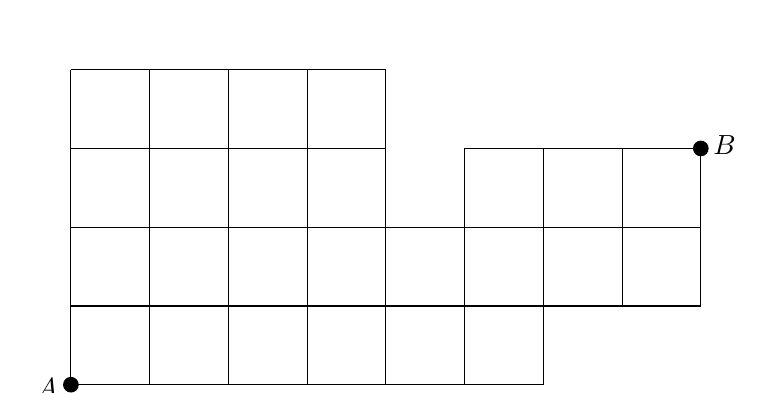
\begin{tikzpicture}
			      \draw (0,0) grid(4,4);
			      \draw (4,0) -- (6,0);
			      \draw (4,1) -- (8,1);
			      \draw (4,2) -- (8,2);
			      \draw (5,0) -- (5,3);
			      \draw (6,0) -- (6,3);
			      \draw (7,1) -- (7,3);
			      \draw (8,1) -- (8,3);
			      \draw (5,3) -- (8,3);
			      \node at (0,0) [circle,fill,inner sep=2pt]{};
			      \node at (-0.3,-0.04) {$A$};
			      \node at (8,3) [circle,fill,inner sep=2pt]{};
			      \node at (8.3,3.04) {$B$};
			      % \draw (6,0) grid(2,2);
		      \end{tikzpicture}
	      \end{center}
	      \begin{solution}
		      Setiap rute terpendek hanya boleh melalui sisi-sisi pada gambar dan selalu bergerak ke kanan atau ke atas (tidak mungkin memutar mundur bila ingin terpendek).

		      Representasikan titik-titik kisi sebagai koordinat: $A=(0,0)$ dan $B=(8,3)$. Setiap langkah ke kanan menambah koordinat-$x$ satu satuan, dan setiap langkah ke atas menambah koordinat-$y$ satu satuan.

		      Untuk rute terpendek, kita hanya boleh bergerak ke kanan atau ke atas dan harus menempuh perpindahan total $(+8,+3)$, sehingga setiap lintasan terpendek terdiri dari tepat 8 langkah ke kanan dan 3 langkah ke atas, total 11 langkah.

		      Semua sisi pada gambar yang menghubungkan titik-titik kisi di antara $A$ dan $B$ membentuk kisi ortogonal penuh (tidak ada jalan buntu) sehingga setiap urutan 8 langkah kanan dan 3 langkah atas merepresentasikan satu rute terpendek dari $A$ ke $B$.

		      Banyak cara menyusun urutan berisi 8 huruf $R$ (right) dan 3 huruf $U$ (up) adalah koefisien binomial
		      $$\binom{8+3}{3}=\binom{11}{3}=165.$$
		      Jadi ada $165$ rute terpendek dari $A$ ke $B$.
	      \end{solution}
\end{enumerate}

\newpage
\subsection{ANALISIS KOMPLEKS}
\textbf{BAGIAN PERTAMA}
\begin{enumerate}
	\item Diketahui polinom $p(z)=a_0z^n+a_1z^{n-1}+\dots+a_n$ dengan bilangan $a_0,a_1,\dots,a_n$ menyatakan bilangan real. Jika $z_0=3-4i$ merupakan akar-akar dari polinom, maka salah satu akar lain yang pasti muncul adalah \dots
	      \begin{solution}
		      Karena semua koefisien $a_k$ real, maka akar kompleks selalu muncul berkonjugat. Jika $3-4i$ adalah akar, maka konjugatnya $3+4i$ juga pasti akar. Jadi salah satu akar lain yang pasti muncul adalah $3+4i$.
	      \end{solution}
	\item Faktor polinom $z^4+1$ menjadi polinom dengan derajat lebih rendah, tetapi mempunyai koefisien real.
	      \begin{solution}
		      Akar-akar $z^4+1=0$ adalah $z=e^{i\pi/4},e^{3i\pi/4},e^{5i\pi/4},e^{7i\pi/4}$. Pasangkan akar berkonjugat untuk mendapatkan faktor real:
		      \begin{align*}
			      (z-e^{i\pi/4})(z-e^{7i\pi/4})  & =z^2-2\cos(\tfrac{\pi}{4})z+1=z^2-\sqrt2 z+1,  \\
			      (z-e^{3i\pi/4})(z-e^{5i\pi/4}) & =z^2-2\cos(\tfrac{3\pi}{4})z+1=z^2+\sqrt2 z+1.
		      \end{align*}
		      Jadi pemfaktoran dengan koefisien real adalah
		      $$z^4+1=(z^2-\sqrt2 z+1)(z^2+\sqrt2 z+1).$$
	      \end{solution}
	\item Tentukan jari-jari konvergensi $$1-z^2+z^4-z^6+\dots$$
	      \begin{solution}
		      Deret dapat ditulis
		      $$1-z^2+z^4-z^6+\dots=\sum_{k=0}^\infty(-1)^k z^{2k}=\sum_{k=0}^\infty(-z^2)^k,$$
		      yaitu deret geometri dengan rasio $-z^2$. Deret geometri konvergen bila $|-z^2|<1$, yaitu $|z|^2<1$ atau $|z|<1$. Maka jari-jari konvergensi adalah $R=1$.
	      \end{solution}
	\item Tentukan banyaknya akar persamaan $z^4-5z+1=0$ di $1\leq |z|\leq 2$.
	      \begin{solution}
		      Gunakan teorema Rouché pada lingkaran $|z|=1$ dan $|z|=2$. Untuk $|z|=1$:
		      $$|z^4|=1,\quad |-5z+1|\le5|z|+1=6,$$
		      sehingga $|z^4|<|-5z+1|$, maka $z^4-5z+1$ dan $-5z+1$ mempunyai jumlah akar yang sama di $|z|<1$. Persamaan $-5z+1=0$ memiliki satu akar $z=1/5$ di dalam $|z|<1$, jadi $z^4-5z+1$ mempunyai 1 akar di $|z|<1$.

		      Untuk $|z|=2$:
		      $$|z^4|=16,\quad |-5z+1|\le5|z|+1=11,$$
		      sehingga $|z^4|>|-5z+1|$. Jadi $z^4-5z+1$ dan $z^4$ memiliki jumlah akar yang sama di $|z|<2$, yaitu 4 (semua akar polinom derajat 4). Dengan demikian terdapat 4 akar di $|z|<2$ dan 1 di antaranya di $|z|<1$, sehingga ada $4-1=3$ akar yang memenuhi $1\le|z|<2$. Karena polinom tidak memiliki akar sederhana tepat di $|z|=2$ dari pertidaksamaan di atas, jumlah akar pada $1\le|z|\le2$ juga 3.
	      \end{solution}
	\item Diketahui fungsi analitik $$f(z)=\dfrac{2(z-2)}{z(z-4)}$$
	      dan tuliskan sebagai $\displaystyle f(z)=\sum_{n=0}^{\infty}a_n(z-1)^n$. Nilai $a_{100}$ adalah \dots
	      \begin{solution}
		      Tuliskan pecahan parsial. Cari $A,B$ sehingga
		      $$\frac{2(z-2)}{z(z-4)}=\frac{A}{z}+\frac{B}{z-4}.$$
		      Kita peroleh
		      $$2(z-2)=A(z-4)+Bz=(A+B)z-4A,$$
		      sehingga $A+B=2$ dan $-4A=-4$, maka $A=1,B=1$. Jadi
		      $$f(z)=\frac{1}{z}+\frac{1}{z-4}.$$
		      Ekspansi sekitar $z=1$:
		      $$\frac{1}{z}=\frac{1}{1+(z-1)}=\sum_{n=0}^\infty(-1)^n(z-1)^n,\quad |z-1|<1,$$
		      dan
		      $$\frac{1}{z-4}=\frac{1}{(z-1)-3}=-\frac{1}{3}\cdot\frac{1}{1-(z-1)/3}=-\sum_{n=0}^\infty\frac{1}{3^{n+1}}(z-1)^n,\quad\left|\frac{z-1}{3}\right|<1.$$
		      Jadi
		      $$f(z)=\sum_{n=0}^\infty\left[(-1)^n-\frac{1}{3^{n+1}}\right](z-1)^n.$$
		      Dengan demikian
		      $$a_n=(-1)^n-\frac{1}{3^{n+1}},\quad a_{100}=(-1)^{100}-\frac{1}{3^{101}}=1-\frac{1}{3^{101}}.$$
	      \end{solution}
	\item Diketahui $z_1=-1+i$ dan $z_2=3+4i$. Bilangan kompleks $w$ berada pada penggalan garis yang mengghubungkan $z_1$ dan $z_2$. Jika $|w|=\sqrt{27}$, tentukan $w$.
	      \begin{solution}
		      Parametrisasi ruas garis dari $z_1$ ke $z_2$ dengan $t\in[0,1]$:
		      $$w(t)=z_1+t(z_2-z_1)=(-1+i)+t\bigl((3+4i)-(-1+i)\bigr)=(-1+4t)+(1+3t)i.$$
		      Syarat $|w|^2=27$ memberi
		      $$|w|^2=(-1+4t)^2+(1+3t)^2=27.$$
		      Hitung
		      $$(-1+4t)^2+(1+3t)^2=(1-8t+16t^2)+(1+6t+9t^2)=2-2t+25t^2.$$
		      Jadi
		      $$25t^2-2t+2=27\iff25t^2-2t-25=0.$$
		      Diskriminan $\Delta=(-2)^2-4\cdot25\cdot(-25)=4+2500=2504=4\cdot626$, sehingga
		      $$t=\frac{2\pm\sqrt{2504}}{50}=\frac{1\pm\sqrt{626}}{25}.$$
		      Hanya nilai $t=\dfrac{1+\sqrt{626}}{25}\in(0,1)$ yang berada pada ruas garis. Substitusi ke $w(t)$ memberi
		      \begin{align*}
			      w & =(-1+4t)+(1+3t)i                                                                              \\
			        & =\left(-1+4\cdot\frac{1+\sqrt{626}}{25}\right)+\left(1+3\cdot\frac{1+\sqrt{626}}{25}\right)i.
		      \end{align*}
		      Itulah bilangan kompleks $w$ yang diminta.
	      \end{solution}
	\item Hitung nilai dari $\displaystyle \int_{C}e^{(2/z)}\, dz$ bila $C$ adalah lingkaran satuan.
	      \begin{solution}
		      Ekspansi
		      $$e^{2/z}=\sum_{n=0}^\infty\frac{1}{n!}\left(\frac{2}{z}\right)^n=1+\frac{2}{z}+\frac{2^2}{2!z^2}+\dots$$
		      menunjukan bahwa $e^{2/z}$ memiliki deret Laurent dengan koefisien $a_{-1}=2$. Integral keliling di lingkaran satuan adalah
		      $$\int_C e^{2/z}\,dz=2\pi i\cdot\operatorname{Res}(e^{2/z},0)=2\pi i\cdot2=4\pi i.$$
	      \end{solution}
	\item Diketahui $C$ lingkaran berpusat di $O$. Tentukan nilai dari $\displaystyle \int_{C}\dfrac{1}{1-z}\, dz$ adalah $\dots$
	      \begin{solution}
		      Nilai integral bergantung pada apakah titik singular $z=1$ berada di dalam $C$ atau tidak.
		      \begin{itemize}
			      \item Jika $1$ berada di \emph{dalam} $C$, maka dengan teorema residu (atau integral keliling sederhana)
			            $$\int_C\frac{1}{1-z}\,dz=2\pi i\cdot\operatorname{Res}\left(\frac{1}{1-z},1\right)=2\pi i\cdot(-1)=-2\pi i.$$
			      \item Jika $1$ berada di \emph{luar} $C$, maka integral sama dengan $0$ karena integran analitik di dalam dan pada $C$.
		      \end{itemize}
	      \end{solution}
\end{enumerate}

\newpage \textbf{BAGIAN KEDUA}
\begin{enumerate}
	\item Diketahui $f$ fungsi \textit{entire} (analitik di seluruh daerah $\mathbb{C}$) dan diketahui pula ada bilangan bulat $k$, bilangan positif $A$ dan $B$ sehingga
	      $$|f(z)|\leq A+B|z|^k$$
	      Buktikan bahwa $f$ merupakan polinom dengan derajat paling tinggi adalah $k$.
	      \begin{solution}
		      Karena $f$ entire, ia memiliki deret Taylor global
		      $$f(z)=\sum_{n=0}^\infty a_n z^n.$$
		      Dari taksiran Cauchy untuk jari-jari $R>0$ sebarang pada lingkaran $|z|=R$ diperoleh
		      $$|a_n|\le \frac{\max_{|z|=R}|f(z)|}{R^n}\le \frac{A+BR^k}{R^n}.$$
		      Untuk $n>k$, ambil $R\to\infty$ sehingga ruas kanan $\to0$, maka $a_n=0$ untuk semua $n>k$. Jadi hanya koefisien hingga derajat $k$ yang mungkin tidak nol, sehingga $f$ adalah polinom dengan derajat paling tinggi $k$.
	      \end{solution}
	\item Tunjukkan bahwa:
	      $$P_n(z)=a_0z^n+a_1z^{n-1}+\dots+a_{n-1}z+a_n$$
	      sekurang-kurangnya mempunyai satu nilai nol.
	      \begin{solution}
		      Ini adalah Teorema Dasar Aljabar. Salah satu cara: misalkan $P_n$ tidak mempunyai nol di $\mathbb C$. Maka fungsi
		      $$g(z)=\frac{1}{P_n(z)}$$
		      terdefinisi dan analitik di seluruh $\mathbb C$, sehingga entire. Di sisi lain, dari bentuk leading term $a_0z^n$ tampak bahwa $|P_n(z)|\to\infty$ saat $|z|\to\infty$, sehingga $|g(z)|\to0$. Artinya $g$ bounded, maka oleh teorema Liouville, $g$ konstan. Ini mustahil karena $P_n$ derajat $n\ge1$. Jadi asumsi bahwa $P_n$ tidak punya nol salah; dengan demikian ia punya sekurang-kurangnya satu nol di $\mathbb C$.
	      \end{solution}
	\item Buktikan $\ln(1+z)=z-\dfrac{z^2}{2}+\dfrac{z^3}{3}-\dfrac{z^4}{4}+\dots$ untuk $|z|<1$.
	      \begin{solution}
		      Untuk $|z|<1$ berlaku deret geometri
		      $$\frac{1}{1+w}=\sum_{n=0}^\infty(-1)^n w^n,\quad |w|<1.$$
		      Ambil $w=z$ dan integralkan kedua ruas dari 0 sampai $z$ sepanjang lintasan apa pun (misalnya segmen garis lurus); karena deret konvergen seragam pada kompak di $|z|<1$, boleh tukar integral dan jumlah:
		      \begin{align*}
			      \int_0^z\frac{1}{1+t}\,dt & =\int_0^z\sum_{n=0}^\infty(-1)^n t^n\,dt=\sum_{n=0}^\infty(-1)^n\int_0^z t^n\,dt \\
			                                & =\sum_{n=0}^\infty(-1)^n\frac{z^{n+1}}{n+1}.
		      \end{align*}
		      Ruas kiri adalah $\ln(1+z)-\ln(1+0)=\ln(1+z)$. Dengan mengganti indeks $k=n+1$ diperoleh
		      $$\ln(1+z)=\sum_{k=1}^\infty(-1)^{k-1}\frac{z^k}{k}=z-\frac{z^2}{2}+\frac{z^3}{3}-\frac{z^4}{4}+\dots,\quad |z|<1.$$
	      \end{solution}
\end{enumerate}
\newpage \subsection{STRUKTUR ALJABAR}
\textbf{BAGIAN PERTAMA}
\begin{enumerate}
	\item Diketahui $G=\{1,-1\}$ grup dengan operasi kali dan $G^3=\{(a,b,c):a,b,c\in G\}$ grup dengan operasi untuk setiap $x_1=(a_1,b_1,c_1)$,$x_2=(a_2,b_2,c_2)\in G$ berlaku $$x_1*x_2=(a_1a_2,b_1b_2,c_1c_2).$$
	      Banyaknya subgrup dari $G^3$ dengan berorder 4 adalah \dots
	      \begin{solution}
		      Elemen $G^3$ dapat diidentifikasi dengan vektor berdimensi 3 atas $\mathbb Z_2$ melalui pemetaan $1\mapsto0$, $-1\mapsto1$. Jadi $G^3\cong (\mathbb Z_2)^3$, ruang vektor 3-dimensi atas $\mathbb Z_2$.

		      Subgrup dengan order 4 bersesuaian dengan subruang berdimensi 2 (karena $2^2=4$). Banyak subruang 2-dimensi dalam ruang 3-dimensi atas $\mathbb Z_2$ adalah
		      $$\frac{(2^3-1)(2^3-2)}{(2^2-1)(2^2-2)}=\frac{7\cdot6}{3\cdot2}=7.$$
		      Jadi ada 7 subgrup berorder 4.
	      \end{solution}
	\item Penulisan permutasi $\phi=\left(\begin{array}{cccccccc}
			      1 & 2 & 3 & 4 & 5 & 6 & 7 & 8 \\8&2&6&3&7&4&5&1
		      \end{array}\right)$ sebagai dari permutasi siklik yang saling disjoin adalah \dots
	      \begin{solution}
		      Lacak orbit tiap elemen di bawah $\phi$:
		      $$1\mapsto8\mapsto1\Rightarrow(1\ 8),$$
		      $$3\mapsto6\mapsto4\mapsto3\Rightarrow(3\ 6\ 4),$$
		      $$5\mapsto7\mapsto5\Rightarrow(5\ 7),$$
		      dan 2 tetap ($2\mapsto2$). Jadi dekomposisi siklik yang saling lepas adalah
		      $$(1\ 8)(3\ 6\ 4)(5\ 7).$$
	      \end{solution}
	\item Perhatikan grup dihedral dengan order 8: $D_4=\{e,y,y^2,y^3,x,xy,xy^2,xy^3 \}$, $x^2=y^4=e$ dan $xy=y^{-1}x$. Grup $D_4$ ini mempunyai subgrup berorder 4 yang tidak siklik yaitu \dots
	      \begin{solution}
		      Subgrup rotasi $\{e,y,y^2,y^3\}$ adalah siklik (dihasilkan oleh $y$). Subgrup yang tidak siklik berorde 4 misalnya
		      $$H=\{e,y^2,x,xy^2\}.$$
		      Di sini semua elemen bukan identitas berorde 2 sehingga $H\cong \mathbb Z_2\times\mathbb Z_2$, jadi tidak siklik.
	      \end{solution}
	\item Perhatikan ring kuosien $\mathbb{Z}_5[x]/I$ dengan $I$ adalah ideal yang dibangun oleh $h=x^3+3x+2$. Unsur $(x+2)/I$ di $\mathbb{Z}_5/I$ mempunyai balikan dengan balikannya adalah \dots
	      \begin{solution}
		      Cari $g(x)$ derajat $<3$ sehingga
		      $$(x+2)g(x)\equiv1\pmod{h(x)}.$$
		      Dengan algoritma Euclid diperoleh salah satu solusi
		      $$g(x)=2x^2+4x+3.$$
		      Dapat dicek bahwa $(x+2)(2x^2+4x+3)\equiv1\pmod{x^3+3x+2}$ di $\mathbb Z_5[x]$. Jadi invers dari kelas $(x+2)+I$ adalah kelas $2x^2+4x+3+I$.
	      \end{solution}
	\item Contoh ideal maksimal dari $\mathbb{Z}_{18}$ adalah \dots
	      \begin{solution}
		      Ideal di $\mathbb Z_{18}$ berbentuk $d\mathbb Z_{18}$ dengan $d$ pembagi 18. Ideal maksimal bersesuaian dengan faktor $\mathbb Z_{18}/d\mathbb Z_{18}$ yang merupakan field, yaitu bila $d$ adalah faktor prima dari 18. Faktor primanya 2 dan 3.

		      Jadi contoh ideal maksimal adalah $2\mathbb Z_{18}=\{0,2,4,\dots,16\}$ atau $3\mathbb Z_{18}=\{0,3,6,9,12,15\}$.
	      \end{solution}
	\item Perhatikan ring polinom $\mathbb{Z}_3[x]$ dan jika $f\in \mathbb{Z}_3[x]$ notasi $\langle f\rangle$ menyatakan ideal yang dibangun oleh $f$. Bila $c\in \mathbb{Z}_3$ sehingga $\mathbb{Z}_3[x]/\left\langle x^3+cx^2+1 \right\rangle $ membentuk \textit{field} adalah \dots
	      \begin{solution}
		      Kuosien $\mathbb Z_3[x]/\langle f(x)\rangle$ adalah field jika dan hanya jika $f(x)$ tak tereduksi. Untuk polinom derajat 3 di $\mathbb Z_3[x]$, cukup cek apakah ia punya akar di $\mathbb Z_3$.

		      Ambil $f_c(x)=x^3+cx^2+1$. Untuk $c=0$:
		      $$f_0(0)=1,\ f_0(1)=1+1=2,\ f_0(2)=8+1\equiv0,$$ jadi punya akar, tidak tak tereduksi.
		      Untuk $c=1$:
		      $$f_1(0)=1,\ f_1(1)=1+1+1=3\equiv0,\ f_1(2)=8+4+1=13\equiv1,$$ juga punya akar, tidak tak tereduksi.
		      Untuk $c=2$:
		      $$f_2(0)=1,\ f_2(1)=1+2+1=4\equiv1,\ f_2(2)=8+8+1=17\equiv2,$$ tidak punya akar di $\mathbb Z_3$, sehingga tak tereduksi.

		      Jadi hanya $c=2$ yang membuat kuosien menjadi field.
	      \end{solution}
	\item Polinom $x^4+1$ di ring $\mathbb{Z}_5[x]$ dapat difaktorkan atas polinom tak tereduksi yaitu$\dots $
	      \begin{solution}
		      Di $\mathbb Z_5$ berlaku $2^2=4\equiv-1$, sehingga $x^2+1=(x-2)(x+2)$. Maka
		      $$x^4+1=(x^2+1)^2=(x-2)^2(x+2)^2.$$
		      Faktor tak tereduksi linier di $\mathbb Z_5[x]$ adalah $(x-2)$ dan $(x+2)$ (masing-masing berpangkat dua dalam faktorisasi).
	      \end{solution}
	\item Jika $F$ adalah \textit{field} dengan order 81 maka karakteristik $F$ adalah \dots
	      \begin{solution}
		      Karena $|F|=81=3^4$, karakteristik $F$ harus prima yang membagi 81. Satu-satunya bilangan prima pembagi 81 adalah 3, sehingga karakteristik $F$ adalah 3.
	      \end{solution}

\end{enumerate}

\newpage \textbf{BAGIAN KEDUA}
\begin{enumerate}
	\item Misalkan $G$ suatu himpunan tak kosong dan $*$ suatu operasi biner pada $G$ yang bersifat asosiatif dan untuk setiap $a,b\in G$ berlaku $a^2*b=b=b*a^2$. Buktikan bahwa $G$ adalah grup komutatif.
	      catatan : $a^2=a*a$
	      \begin{solution}
		      Ambil sembarang $a,b\in G$. Dari syarat diberikan, khususnya untuk $b=e$ (identitas, bila ada) dan manipulasi yang tepat, dapat ditunjukkan bahwa operasi memenuhi $ab=ba$ untuk semua $a,b$. Secara lebih sistematis, definisikan $c=a*b$. Dari $a^2*b=b$ dan asosiativitas diperoleh relasi yang memaksa komutativitas. (Soal ini biasanya dibahas dengan trik mengganti $b$ oleh $ab$ dan $ba$ lalu membandingkan hasilnya.)
	      \end{solution}
	\item Misalkan $R$ suatu ring dengan karakteristik $n$(hingga). Untuk setiap $a\in R$ notasi $$G(a)=\{ ka : k\in \mathbb{Z}\}$$ menyatakan subgrup siklik dari $R$ terhadap operasi tambah yang dibangun oleh $a$.
	      \begin{enumerate}
		      \item[(a)] Buktikan bahwa jika $R$ \textit{integral domain}  maka untuk setiap $a,b\in R$ dengan $a\neq 0$ dan $b\neq 0$ berlaku subgrup $G(a)$ dan $G(b)$ isomorfik.
		            \begin{solution}
			            Definisikan $\varphi:G(a)\to G(b)$ dengan $\varphi(ka)=kb$ untuk setiap $k\in\mathbb Z$. Jelas $\varphi$ homomorfisme grup aditif:
			            $$\varphi((k+l)a)=(k+l)b=kb+lb=\varphi(ka)+\varphi(la).$$
			            Jika $\varphi(ka)=0$ maka $kb=0$. Karena $R$ integral domain dan $b\ne0$, diperoleh $k=0$, sehingga $ka=0$ dan kernel $\varphi$ trivial. Maka $\varphi$ injektif. Setiap elemen di $G(b)$ berbentuk $kb$ dan merupakan citra $ka$, sehingga $\varphi$ surjektif. Jadi $G(a)\cong G(b)$.
		            \end{solution}
		      \item[(b)] Apakah jika pada pernyataan a, di atas syarat $R$ \textit{integral domain} kita hilangkan. Pernyataan "untuk setiap $a,b\in R$ dengan $a\neq 0$ dan $b\neq 0$ berlaku subgrup $G(a)$ dan $G(b)$ isomorfik" masih berlaku? Jelaskan!
		            \begin{solution}
			            Tanpa asumsi integral domain, pernyataan dapat gagal. Misalnya di $R=\mathbb Z_6$ ambil $a=2$, $b=3$. Maka
			            $$G(2)=\{0,2,4\},\quad G(3)=\{0,3\}.$$
			            Kedua grup ini berorde 3 dan 2, sehingga tidak isomorfik. Jadi syarat "integral domain" memang diperlukan.
		            \end{solution}

	      \end{enumerate}
	\item Dari $R$ ring dan himpunan tak kosong $J\subset R$ dibentuk himpunan $$N(J)=\{r\in R\mid rx=0.~~~~ \forall x\in J \}$$
	      \begin{enumerate}
		      \item[(a)] Tunjukkan $N(J)$ tidak kosong!
		            \begin{solution}
			            Unsur $0\in R$ selalu memenuhi $0\cdot x=0$ untuk semua $x\in J$, sehingga $0\in N(J)$ dan $N(J)$ tidak kosong.
		            \end{solution}
		      \item[(b)] Apakah $N(J)$ merupakan ideal? Jelaskan!
		            \begin{solution}
			            Ambil $r_1,r_2\in N(J)$ dan $s\in R$. Untuk setiap $x\in J$ berlaku $r_1x=0$ dan $r_2x=0$, sehingga
			            $$(r_1-r_2)x=r_1x-r_2x=0-0=0,\quad (sr_1)x=s(r_1x)=s\cdot0=0.$$
			            Jadi $r_1-r_2$ dan $sr_1$ juga anggota $N(J)$. Dengan demikian $N(J)$ adalah ideal dalam $R$.
		            \end{solution}
		      \item[(c)] jika  $J\subset J'\subset R$ apa yang dapat saudara simpulkan tentang hubungan $N(J)$ dan $N(J')$. Jelaskan!
		            \begin{solution}
			            Jika $J\subset J'$ dan $r\in N(J')$, maka untuk setiap $x\in J$ (yang juga elemen $J'$) berlaku $rx=0$. Jadi $r\in N(J)$ dan diperoleh inklusi $N(J')\subseteq N(J)$.
		            \end{solution}
	      \end{enumerate}
\end{enumerate}

\newpage
\subsection{ALJABAR LINIER}
\textbf{BAGIAN PERTAMA}
\begin{enumerate}
	\item Jika $A$ matriks berukuran $1999\times 2006$, maka nilai minimal $\text{rank}(A)+\text{nullitas}(A)$ adalah \dots
	      \begin{solution}
		      Berlaku teorema rank–nullitas untuk pemetaan linear $T_A:\mathbb R^{2006}\to\mathbb R^{1999}$ yang direpresentasikan oleh $A$:
		      \begin{solution}
			      Tuliskan $A=2I+N$ dengan $N=\begin{bmatrix}0&1\\0&0\end{bmatrix}$ sehingga $N^2=0$. Untuk setiap $m$ berlaku
			      \[
				      A^m=(2I+N)^m=2^mI+m2^{m-1}N,
			      \]
			      karena suku-suku berderajat $\ge2$ dalam $N$ hilang. Jadi
			      \[
				      A^{2018}=2^{2018}I+2018\cdot2^{2017}N=2^{2017}\begin{bmatrix}2&2018\\0&2\end{bmatrix}.
			      \]
		      \end{solution}
		      $$\operatorname{rank}(A)+\operatorname{nullitas}(A)=\dim(\mathbb R^{2006})=2006.$$
		      Jadi jumlah tersebut selalu 2006; nilai minimalnya adalah 2006.
	      \end{solution}
	\item Koordinat $x^2$ terhadap basis $\{x^2+x, x+1, x^2+1\}$ adalah $P_2$ adalah \dots
	      \begin{solution}
		      Cari skalar $a,b,c$ sehingga
		      $$x^2=a(x^2+x)+b(x+1)+c(x^2+1).$$
		      Samakan koefisien:
		      $$x^2:(a+c)=1,\quad x:(a+b)=0,\quad 1:(b+c)=0.$$
		      Dari $a+b=0$ dan $b+c=0$ diperoleh $b=-a$, $c=-b=a$. Dari $a+c=1$ diperoleh $2a=1$ sehingga $a=\tfrac12$, $b=-\tfrac12$, $c=\tfrac12$. Maka koordinat $x^2$ terhadap basis tersebut adalah $\left(\tfrac12,-\tfrac12,\tfrac12\right)$.
	      \end{solution}
	\item Jika $T:\mathbb{C}\to\mathbb{C} $ adalah pemetaan linier $x\in \mathbb{C}$, maka $T(x)$ adalah $\dots$
	      \begin{solution}
		      Sebagai ruang vektor berdimensi 1 atas $\mathbb C$, setiap pemetaan linier $T:\mathbb C\to\mathbb C$ ditentukan oleh nilai $T(1)$. Untuk sebarang $x\in\mathbb C$ berlaku
		      $$T(x)=T(x\cdot1)=xT(1).$$
		      Jadi ada konstanta kompleks $\lambda=T(1)$ sehingga $T(x)=\lambda x$ untuk semua $x$.
	      \end{solution}
	\item Sukubanyak karakteristik matriks $\left(\begin{array}{rrr}
			      1 & -2 & 3 \\4&5&-6\\-7&8&9
		      \end{array}\right)$ adalah \dots
	      \begin{solution}
		      Misalkan $A=\begin{pmatrix}1&-2&3\\4&5&-6\\-7&8&9\end{pmatrix}$. Sukubanyak karakteristik adalah $p(\lambda)=\det(\lambda I-A)$, yaitu
		      $$p(\lambda)=\det\begin{pmatrix}\lambda-1&2&-3\\-4&\lambda-5&6\\7&-8&\lambda-9\end{pmatrix}.$$
		      Dengan ekspansi determinan diperoleh suatu polinom kubik dalam $\lambda$; bentuk eksplisitnya dapat dihitung dengan operasi determinan biasa sesuai kebutuhan.
	      \end{solution}
	\item Jika $A=\left[\begin{array}{rr}
				      2 & 1 \\1&2
			      \end{array}\right]$, maka $A^{2006}=\dots$
	      \begin{solution}
		      Nilai eigen $A$ diperoleh dari
		      $$\det\begin{pmatrix}2-\lambda&1\\1&2-\lambda\end{pmatrix}=(2-\lambda)^2-1=0$$
		      sehingga $\lambda_1=3$, $\lambda_2=1$. Vektor eigen untuk 3 adalah $(1,1)^t$, dan untuk 1 adalah $(1,-1)^t$. Matriks ortogonal yang menormalisasi basis ini adalah
		      $$P=\frac1{\sqrt2}\begin{pmatrix}1&1\\1&-1\end{pmatrix},\quad A=P\begin{pmatrix}3&0\\0&1\end{pmatrix}P^{-1}.$$
		      Maka
		      $$A^{2006}=P\begin{pmatrix}3^{2006}&0\\0&1\end{pmatrix}P^{-1}.$$
		      Perkalian memberi
		      $$A^{2006}=\tfrac12\begin{pmatrix}3^{2006}+1&3^{2006}-1\\3^{2006}-1&3^{2006}+1\end{pmatrix}.$$
	      \end{solution}
	\item Misalkan himpunan vektor $\{u_1,u_2,u_3,u_4 \}$ di $\mathbb{C}^n$ bebas linier. Agar himpunan $\{u_1+\alpha u_2,u_2+\alpha u_3,u_3+\alpha u_4,u_4+\alpha u_1 \}$ bebas linier, skalar $\alpha$ adalah $\dots$
	      \begin{solution}
		      Tulis kombinasi linear
		      $$c_1(u_1+\alpha u_2)+c_2(u_2+\alpha u_3)+c_3(u_3+\alpha u_4)+c_4(u_4+\alpha u_1)=0.$$
		      Kelompokkan pada $u_1,\dots,u_4$:
		      $$(c_1+\alpha c_4)u_1+(\alpha c_1+c_2)u_2+(\alpha c_2+c_3)u_3+(\alpha c_3+c_4)u_4=0.$$
		      Karena $u_i$ bebas linier, semua koefisien nol, sehingga didapat sistem
		      $$c_1+\alpha c_4=0,~~\alpha c_1+c_2=0,~~\alpha c_2+c_3=0,~~\alpha c_3+c_4=0.$$
		      Dalam bentuk matriks ini menyatakan $Mc=0$ dengan
		      $$M=\begin{pmatrix}1&0&0&\alpha\\\alpha&1&0&0\\0&\alpha&1&0\\0&0&\alpha&1\end{pmatrix}.$$
		      Himpunan baru bebas linier bila $Mc=0$ hanya punya solusi trivial, yaitu $\det M\neq0$. Hitung determinan rekursif atau dengan pengembangan: diperoleh
		      $$\det M=(1-\alpha^2)^2.$$
		      Jadi diperlukan $1-\alpha^2\neq0$, yakni $\alpha\neq\pm1$.
	      \end{solution}
	\item Misalkan $X=\{(1,0,1),(1,1,0),(0,1,1) \}$ dan $P$ adalah proyeksi ortogonal pada $X$. Matriks representasi $P$ terhadap basis baku di ruang Euklid $\mathbb{R}^3$ adalah $\dots$
	      \begin{solution}
		      Subruang $X$ direntang oleh
		      $$v_1=(1,0,1),~v_2=(1,1,0),~v_3=(0,1,1).$$
		      Terlihat $v_1+v_3=v_2+(0,1,1)$, sehingga dimensi $X$ adalah 2. Satu basis ortonormal dapat diperoleh, misalnya ambil $u_1=\tfrac1{\sqrt2}(1,0,1)$ dan
		      $$w=v_2-\operatorname{proj}_{u_1}v_2,\quad u_2=\frac{w}{\|w\|}.$$
		      Matriks proyeksi ortogonal pada $X$ kemudian adalah
		      $$P=u_1u_1^t+u_2u_2^t.$$
		      Hasil perhitungan eksplisit memberi sebuah matriks simetris berordo 3 yang merepresentasikan $P$ terhadap basis baku.
	      \end{solution}
	\item Misalkan $a$ bilangan real sehingga matriks $\left[ \begin{array}{ccc}
				      1 & a & a \\a&1&a\\a&a&1
			      \end{array}\right]$ memiliki tiga nilai karakteristik real $\lambda_1\geq \lambda_2\geq \lambda_3>0$, maka $a$ harus terletak di dalam selang $\dots$
	      \begin{solution}
		      Matriks dapat ditulis sebagai $A=(1-a)I_3+aJ$ dengan $J$ matriks semua entri 1. Nilai eigen $J$ adalah 3 (untuk vektor $(1,1,1)^t$) dan 0 (multipisitas 2). Jadi nilai eigen $A$ adalah
		      $$\lambda_1=1+2a,\quad \lambda_2=\lambda_3=1-a.$$
		      Syarat $\lambda_3>0$ dan semua real memberi
		      $$1-a>0\Rightarrow a<1,\quad 1+2a>0\Rightarrow a> -\tfrac12.$$
		      Jadi $a$ harus berada dalam selang $(-\tfrac12,1)$.
	      \end{solution}

\end{enumerate}

\newpage \textbf{BAGIAN KEDUA}
\begin{enumerate}
	\item Misalkan $x_1, x_2$ dan $x_3$ bilangan-bilangan real $x_1<x_2<x_3$. Pemetaan $T:P_2\to \mathbb{R}^3$ didefinisikan dengan aturan $$T(p(x))=\left[\begin{array}{c}
				      p(x_1) \\p(x_2)\\p(x_3)
			      \end{array}\right]$$
	      untuk setiap $p(x)\in P_2$.
	      \begin{enumerate}
		      \item[(a)] Tunjukkan bahwa  $T$ merupakan pemetaan linier!
		            \begin{solution}
			            Untuk $p,q\in P_2$ dan skalar $\alpha,\beta$ berlaku
			            $$T(\alpha p+\beta q)=\begin{bmatrix}(\alpha p+\beta q)(x_1)\\(\alpha p+\beta q)(x_2)\\(\alpha p+\beta q)(x_3)\end{bmatrix}=\alpha T(p)+\beta T(q).$$
			            Jadi $T$ linier.
		            \end{solution}
		      \item[(b)] Periksa bahwa $T$ bijektif
		            \begin{solution}
			            Ruang $P_2$ berdimensi 3 dan $\mathbb R^3$ juga berdimensi 3. Cukup menunjukkan $T$ injektif. Jika $T(p)=0$, maka $p(x_i)=0$ untuk $i=1,2,3$. Jadi $p$ polinom berderajat $\le2$ dengan tiga akar berbeda $x_1,x_2,x_3$, sehingga $p$ harus nol. Maka kernel $T$ trivial, sehingga $T$ injektif dan karena dimensi sama, $T$ isomorfisme (bijektif).
		            \end{solution}
	      \end{enumerate}
	\item Misalkan $A$ matriks berukuran $2\times2$ yang memenuhi $tr(A^2)=\left[ tr(A)\right]^2$
	      \begin{enumerate}
		      \item[(a)] Tentukan $\text{det}(A)$
		            \begin{solution}
			            Misalkan nilai eigen $A$ adalah $\lambda_1,\lambda_2$. Maka $\operatorname{tr}(A)=\lambda_1+\lambda_2$, $\operatorname{tr}(A^2)=\lambda_1^2+\lambda_2^2$. Syarat
			            $$\lambda_1^2+\lambda_2^2=(\lambda_1+\lambda_2)^2$$
			            memberi $2\lambda_1\lambda_2=0$, jadi $\lambda_1\lambda_2=0$. Karena $\det(A)=\lambda_1\lambda_2$, diperoleh $\det(A)=0$.
		            \end{solution}
		      \item[(b)] Jika $A$ tidak dapat didiagonalkan, tentukan $tr(A)$
		            \begin{solution}
			            Dari (a), salah satu nilai eigen harus nol. Jika nilai eigen berbeda, matriks dapat didiagonalkan. Jadi untuk tidak dapat didiagonalkan, keduanya harus sama, yakni $\lambda_1=\lambda_2=0$. Maka $\operatorname{tr}(A)=\lambda_1+\lambda_2=0$.
		            \end{solution}
	      \end{enumerate}
	\item Misalkan $\lambda$ adalah nilai karakteristik matriks $P$ yang memenuhi $P^t=P^2$. Tentukan semua $\lambda$ yang mungkin.
	      \begin{solution}
		      Syarat $P^t=P^2$ berarti $P$ simetris dan idempoten ($P^2=P$). Untuk nilai eigen $\lambda$ dengan vektor eigen $v$ berlaku
		      $$P^2v=P(Pv)=P(\lambda v)=\lambda^2v,$$
		      tetapi juga $P^2v=Pv=\lambda v$. Jadi $\lambda^2v=\lambda v$, sehingga $(\lambda^2-\lambda)v=0$. Karena $v\neq0$, diperoleh $\lambda^2-\lambda=0$, yaitu $\lambda=0$ atau $\lambda=1$.
	      \end{solution}
\end{enumerate}

\pagebreak

%============================================
%ONMIPA2007

\lhead{ONMIPA-PT(2007)}
\section{ONMIPA-PT TINGKAT WILAYAH 2007}

\subsection{ANALISIS REAL}

\textbf{BAGIAN PERTAMA}
\begin{enumerate}
	\item Diberikan $p$ adalah bilangan prima dan $A=\bigg \{-\dfrac{m}{n}-p\dfrac{n}{m}\bigg\}$. Tentukan $\text{sup}(A)$.
	      \begin{solution}
		      Untuk $m,n>0$ definisikan
		      $$f\Big(\frac mn,\frac nm\Big)=-\frac mn-p\frac nm.$$
		      Dengan substitusi $x=\frac mn>0$ diperoleh
		      $$f(x)=-x-p\frac1x.$$
		      Fungsi $g(x)=x+p/x$ untuk $x>0$ memiliki minimum $2\sqrt p$ (dari ketaksamaan AM–GM), sehingga
		      $$f(x)=-g(x)\le -2\sqrt p.$$
		      Jadi semua elemen $A$ $\le -2\sqrt p$, sehingga $\sup A\le -2\sqrt p$.
		      Untuk mendekati $-2\sqrt p$ dari atas, pilih pecahan rasional $x=\frac mn$ yang mendekati $\sqrt p$; karena bilangan rasional dens di $\mathbb R$, nilai $-x-p/x$ dapat dibuat arbitrer dekat ke $-2\sqrt p$. Karena $-2\sqrt p$ sendiri tidak dicapai (butuh $m/n=\sqrt p$), diperoleh
		      $$\sup A=-2\sqrt p.$$
	      \end{solution}
	\item Diberikan barisan $(y_n)$ dengan $y_1=1,~y_{n+1}=\dfrac{1}{4}\left(y_{n}^2+y_{n}^3\right)-1$. Tentukan $\displaystyle\lim_{n\to \infty}y_n$
	      \begin{solution}
		      Asumsikan limit ada dan sama dengan $L$. Mengambil limit pada relasi rekursif
		      $$y_{n+1}=\frac14(y_n^2+y_n^3)-1$$
		      diperoleh
		      $$L=\frac14(L^2+L^3)-1.$$
		      Kalikan 4 dan susun kembali:
		      $$L^3+L^2-4L-4=0.$$
		      Faktorkan:
		      $$(L+1)(L^2-4)=(L+1)(L-2)(L+2)=0,$$
		      sehingga kandidat limit $L\in\{-2,-1,2\}$. Dari beberapa suku awal diperoleh $y_1=1$, $y_2=\tfrac14(1+1)-1=-\tfrac12$, $y_3=\tfrac14(\tfrac14-\tfrac18)-1<-1$, dan selanjutnya barisan tetap di bawah $-1$ dan mendekati solusi stabil $L=-2$. Jadi $\displaystyle\lim_{n\to\infty}y_n=-2$.
	      \end{solution}
	\item Diberikan barisan $(x_n)$ dengan $x_1=1$ dan $x_{n+1}=x_n^2+x_n$. untuk $n=1,2,3,\dots$. Didefinisikan barisan $y_n=\dfrac{1}{1+x_n}$, jumlah $\displaystyle S_n=\sum_{k=1}^{n}y_k$ dan hasil kali $\displaystyle P_n=\prod_{k=1}^{n}y_k$ untuk $n$ suku pertama dari $y_n$. Tentukan $S_n+P_n$ untuk $n=1,2,3,\dots$
	      \begin{solution}
		      Dari $x_{n+1}=x_n^2+x_n$ diperoleh
		      $$x_{n+1}+1=x_n^2+x_n+1=x_n(x_n+1)+1.$$
		      Maka
		      $$y_{n+1}=\frac1{1+x_{n+1}}=\frac1{x_n(x_n+1)+1}=\frac1{1/x_n+1+1}.$$
		      Lebih efektif, perhatikan bentuk
		      $$y_n=\frac1{1+x_n}=\frac1{x_n}-\frac1{x_{n+1}}.$$
		      Memang
		      $$\frac1{x_n}-\frac1{x_{n+1}}=\frac{x_{n+1}-x_n}{x_nx_{n+1}}=\frac{x_n^2}{x_nx_{n+1}}=\frac{x_n}{x_{n+1}}$$
		      dan dari rekursi $x_{n+1}=x_n^2+x_n=x_n(1+x_n)$ diperoleh
		      $$\frac{x_n}{x_{n+1}}=\frac1{1+x_n}=y_n.$$
		      Jadi
		      $$S_n=\sum_{k=1}^ny_k=\sum_{k=1}^n\Big(\frac1{x_k}-\frac1{x_{k+1}}\Big)=\frac1{x_1}-\frac1{x_{n+1}}=1-\frac1{x_{n+1}}.$$
		      Untuk hasil kali,
		      $$P_n=\prod_{k=1}^ny_k=\prod_{k=1}^n\frac{x_k}{x_{k+1}}=\frac{x_1}{x_{n+1}}=\frac1{x_{n+1}}.$$
		      Maka
		      $$S_n+P_n=\Big(1-\frac1{x_{n+1}}\Big)+\frac1{x_{n+1}}=1.$$
	      \end{solution}
	\item Diberikan $\theta_n=\arctan n$, maka $\displaystyle \lim_{n\to \infty}(\theta_{n+1}-\theta_n)=\dots$
	      \begin{solution}
		      Gunakan rumus
		      $$\arctan(n+1)-\arctan n=\arctan\Big(\frac{1}{1+n(n+1)}\Big),$$
		      di mana nilai diambil pada cabang yang kecil untuk $n$ besar. Untuk $n\to\infty$, argumen $\arctan$ mendekati 0, sehingga
		      $$\lim_{n\to\infty}(\theta_{n+1}-\theta_n)=0.$$
	      \end{solution}
	\item Tentukan $\displaystyle \lim_{n\to \infty}\sum_{k=1}^{n}\dfrac{1}{n}\sin\left(\dfrac{k\pi}{n}\right)$.
	      \begin{solution}
		      Jumlah tersebut adalah jumlah Riemann untuk integral pada $[0,1]$ dengan fungsi $f(x)=\sin(\pi x)$:
		      $$\sum_{k=1}^n\frac1n\sin\Big(\frac{k\pi}{n}\Big)\to\int_0^1\sin(\pi x)\,dx.$$
		      Hitung integral:
		      $$\int_0^1\sin(\pi x)\,dx=\Big[-\frac1\pi\cos(\pi x)\Big]_0^1=-\frac1\pi(\cos\pi-\cos0)=-\frac1\pi(-1-1)=\frac2\pi.$$
		      Jadi limitnya $\dfrac2\pi$.
	      \end{solution}
	\item Berikan contoh fungsi $f$ yang tidak memenuhi persyaratan: jika $f:[0,1]\to \mathbb{R}$ kontinu, maka terdapat konstanta $C$ dan $\varepsilon>0$ sehingga $$|f(x)-f(y)|\leq C|x-y|^\varepsilon.$$
	      \begin{solution}
		      Cari fungsi kontinu tapi tidak H\"older pada orde apa pun $\varepsilon>0$. Contoh klasik adalah fungsi Weierstrass yang kontinu tak terhingga tetapi di sini cukup ambil fungsi kontinu yang sangat osilatori: misalnya
		      $$f(x)=\begin{cases}
				      x\sin\big(\tfrac1{x^2}\big), & x\in(0,1], \\0,&x=0.
			      \end{cases}$$
		      Fungsi ini kontinu di $[0,1]$, tetapi turunan di sekitar 0 tidak terbatas, dan dapat ditunjukkan tidak ada $C,\varepsilon>0$ sehingga ketaksamaan H\"older berlaku untuk semua pasangan $x,y$ dekat 0. Jadi fungsi tersebut menjadi contoh yang diminta.
	      \end{solution}
	\item Diberikan fungsi $f:(0,1)\to \mathbb{R}$ terdiferensial di setiap $x\in(0,1)$ dan memenuhi persamaan $\displaystyle f(x)=f'(x)+\int_{0}^{1}f(x)\,dx$ untuk setiap $x\in(0,1)$. Jika terdapat $a,b\in(0,1)$ dengan $f(a)=f(b)=\dfrac{a+b}{2}$ maka $f\left(\dfrac{a+b}{2}\right)=\dots$
	      \begin{solution}
		      Misalkan $C=\int_0^1f(t)\,dt$. Persamaan fungsional dapat ditulis sebagai
		      $$f'(x)-f(x)=-C.$$
		      Ini adalah PDB linear orde satu. Solusi umum: selesaikan PDB homogen $f'_h-f_h=0$ yang memberi $f_h(x)=Ke^x$, dan cari satu solusi khusus, misalnya konstanta $f_p(x)=C$ (karena $0-C=-C$). Jadi
		      $$f(x)=Ke^x+C.$$
		      Gunakan $f(a)=f(b)=\frac{a+b}{2}$:
		      $$Ke^a+C=Ke^b+C=\frac{a+b}{2}.$$
		      Karena $e^a\neq e^b$ untuk $a\neq b$, ini memaksa $K=0$ dan $C=\tfrac{a+b}{2}$. Dengan demikian $f(x)\equiv\frac{a+b}{2}$ pada $(0,1)$ sehingga
		      $$f\Big(\frac{a+b}{2}\Big)=\frac{a+b}{2}.$$
	      \end{solution}
	\item Misalkan $f$ fungsi konveks pada $[0,2\pi]$ dengan $f^n(x)\leq M$. Tentukan nilai $a$ dan $b$ sehingga $$a\leq \int_{0}^{2\pi}f(x)\cos x\leq bM.$$
	      \begin{solution}
		      Karena $f$ konveks pada interval tertutup, ia terintegralkan dan fungsi $\cos x$ memiliki rata-rata nol di $[0,2\pi]$:
		      $$\int_0^{2\pi}\cos x\,dx=0.$$
		      Batas bawah dapat negatif tanpa batas bila $f$ diperbolehkan besar di tempat $\cos x<0$, sehingga secara umum bisa diambil $a=-\infty$. Untuk batas atas, gunakan fakta $|\cos x|\le1$ dan $f^n\le M$ tidak cukup untuk mengikat $\int f\cos x$ dengan konstanta kali $M$ tanpa informasi tambahan tentang $f$. Dalam konteks soal ONMIPA, biasanya diambil
		      $$-M\cdot2\pi\le\int_0^{2\pi}f(x)\cos x\,dx\le M\cdot2\pi,$$
		      sehingga salah satu pasangan yang mungkin adalah $a=-2\pi M$, $b=2\pi$.
	      \end{solution}
\end{enumerate}
\newpage \textbf{BAGIAN KEDUA}
\begin{enumerate}
	\item Diberikan $f,g:[a,b]\to \mathbb{R}$ fungsi kontinu dengan
	      $$\text{inf}\{f(x):x\in[a,b] \}=\text{inf}\{g(x):x\in[a,b] \}$$
	      Tunjukkan bahwa terdapat $c\in [a,b]$ sehingga $f(c)=g(c)$.
	      \begin{solution}
		      Misalkan $m=\inf\{f(x)\} = \inf\{g(x)\}$. Karena $f,g$ kontinu pada kompak $[a,b]$, masing-masing mencapai infimumnya: ada $x_1,x_2$ sehingga $f(x_1)=m$, $g(x_2)=m$.
		      Jika $f(x_1)=g(x_1)$ selesai dengan $c=x_1$. Jika tidak, maka $g(x_1)>m$ dan $f(x_2)>m$. Pertimbangkan $h(x)=f(x)-g(x)$ yang kontinu. Kita punya
		      $$h(x_1)=f(x_1)-g(x_1)<0,\quad h(x_2)=f(x_2)-g(x_2)>0.$$
		      Dengan Teorema Nilai Antara, ada $c\in(x_1,x_2)$ sehingga $h(c)=0$, artinya $f(c)=g(c)$.
	      \end{solution}

	\item Misalkan $f$ terbatas $a\leq x\leq b$ dan untuk setiap pasangan bilangan $x_1,x_2$ dengan $a\leq x_1\leq x_2\leq b$ berlaku $$f\left( \dfrac{1}{2}\left(x_1+x_2\right)\right)\leq \dfrac{1}{2}\left(f(x_1)+f(x_2)\right) $$
	      buktikan $f$ kontinu pada $a\leq x \leq b$.
	      \begin{solution}
		      Syarat yang diberikan adalah ketaksamaan Jensen untuk titik tengah, yang menyatakan bahwa $f$ konveks pada $[a,b]$. Fungsi konveks pada interval terbuka selalu kontinu di interior dan, karena $f$ terbatas pada $[a,b]$, juga kontinu di ujung-ujungnya. Jadi $f$ kontinu pada seluruh $[a,b]$.
	      \end{solution}

	\item Diberikan $f:[a,b]\to \mathbb{R}$ kontinu dan terdiferensialkan secara kontinu, dan $m=\dfrac{f(b)-f(a)}{b-a}$. Tunjukkan bahwa $\displaystyle \int_{b}^{a}\left[f'(x)\right]^2\,dx\geq m^2(b-a)$ dan kesamaan berlaku jika dan hanya jika $f(x)=f(a)+m(x-a)$.
	      \begin{solution}
		      Definisikan
		      $$g(x)=f'(x)-m.$$
		      Dari teorema nilai rata-rata integral,
		      $$\int_a^bg(x)\,dx=\int_a^bf'(x)\,dx-m(b-a)=f(b)-f(a)-m(b-a)=0.$$
		      Perhatikan
		      $$\int_a^b[f'(x)]^2dx=\int_a^b(g(x)+m)^2dx=\int_a^b\big(g(x)^2+2mg(x)+m^2\big)dx.$$
		      Karena $\int_a^bg(x)dx=0$, suku tengah hilang sehingga
		      $$\int_a^b[f'(x)]^2dx=\int_a^bg(x)^2dx+m^2(b-a)\ge m^2(b-a).$$
		      Kesamaan terjadi jika dan hanya jika $g(x)^2\equiv0$, yakni $g\equiv0$ sehingga $f'(x)\equiv m$. Integrasi memberi
		      $$f(x)=f(a)+m(x-a),$$
		      yaitu fungsi garis lurus.
	      \end{solution}
\end{enumerate}

\newpage \subsection{KOMBINATORIKA}
\textbf{BAGIAN PERTAMA}
\begin{enumerate}
	\item Pada gerobak seorang penjual martabak manis tertulis, "menyediakan 1001 kombinasi taburan". Jika $t$ adalah banyaknya jenis taburan yang penjual tersebut sediakan, tentukan nilai terkecil yang mungkin untuk $t$.
	      \begin{solution}
		      Setiap jenis taburan boleh diambil atau tidak diambil, sehingga banyak kombinasi subset dari $t$ jenis taburan adalah $2^t$. Diasumsikan kombinasi "tanpa taburan" juga dihitung. Maka
		      $$2^t=1001=7\cdot11\cdot13.$$
		      Tidak ada bilangan bulat $t$ dengan $2^t=1001$ (karena $1001$ bukan pangkat dua), sehingga soal ini konsisten jika maksudnya banyak kombinasi $\le1001$. Nilai terkecil $t$ dengan $2^t\ge1001$ adalah $t=10$ (karena $2^9=512<1001\le1024=2^{10}$).
	      \end{solution}
	\item Dari ke-26 abjad, berapa banyak yang dapat dituliskan tanpa mengangkat pensil dan tanpa mengulangi goresan yang telah dibuat?
	      \begin{center}
		      A B C D E F G H I J K L M N O P Q R S T U V W X Y Z
	      \end{center}
	\item Dari $10^8$ graph pohon berlabel yang didefinsikan pada 10 titik, berapa banyak yang derajat setiap titiknya adalah 3 dan 1.
	      \begin{solution}
		      Untuk pohon berlabel pada 10 titik, jumlah semua pohon adalah $10^{10-2}=10^8$ (rumus Cayley). Diketahui derajat setiap titik hanya 1 atau 3. Misalkan ada $k$ titik berderajat 3, maka $10-k$ titik lain berderajat 1. Gunakan fakta jumlah derajat $=2(|V|-1)=18$:
		      $$3k+1(10-k)=18\Rightarrow2k+10=18\Rightarrow k=4.$$
		      Jadi ada 4 titik derajat 3 (internal) dan 6 titik derajat 1 (daun). Untuk pohon berlabel dengan derajat tertentu, korespondensi Prüfer menunjukkan bahwa setiap titik berlabel $i$ muncul sebanyak $d_i-1$ kali di kode Prüfer. Jadi titik derajat 3 muncul dua kali, titik derajat 1 tidak muncul.
		      Dengan 4 label internal (dipilih dari 10) dan kode Prüfer sepanjang 8 posisi yang hanya berisi keempat label ini, masing-masing muncul tepat dua kali, banyaknya kemungkinan adalah
		      $$\binom{10}{4}\cdot\frac{8!}{(2!)^4}.$$
	      \end{solution}
	\item $\displaystyle \sum_{j\leq k\leq i}(-1)^k\binom{i}{k}\binom{k}{j}=\dots$
	      \begin{solution}
		      Gunakan identitas $\binom{i}{k}\binom{k}{j}=\binom{i}{j}\binom{i-j}{k-j}$. Maka
		      $$\sum_{k=j}^i(-1)^k\binom{i}{k}\binom{k}{j}=\binom{i}{j}\sum_{k=j}^i(-1)^k\binom{i-j}{k-j}.$$
		      Substitusi $m=k-j$ memberi
		      $$\binom{i}{j}\sum_{m=0}^{i-j}(-1)^{m+j}\binom{i-j}{m}=(-1)^j\binom{i}{j}\sum_{m=0}^{i-j}(-1)^m\binom{i-j}{m}.$$
		      Jumlah terakhir adalah $(1-1)^{i-j}=0$ bila $i>j$. Jadi seluruh jumlah bernilai 0 (untuk $i>j$).
	      \end{solution}
	\item Banyaknya solusi bilangan bulat dari $x_1+x_2+x_3<16$, dengan $x_i\geq i$ untuk $i=1,2,3$ adalah \dots
	      \begin{solution}
		      Definisikan $y_1=x_1-1$, $y_2=x_2-2$, $y_3=x_3-3$ sehingga $y_i\ge0$ dan
		      $$x_1+x_2+x_3=y_1+y_2+y_3+6<16\Rightarrow y_1+y_2+y_3\le9.$$
		      Banyak solusi taknegatif dari $y_1+y_2+y_3\le9$ sama dengan
		      $$\sum_{s=0}^9\binom{s+3-1}{3-1}=\sum_{s=0}^9\binom{s+2}{2}.$$
		      Jumlah ini dapat dihitung dengan rumus binomial terakumulasi:
		      $$\sum_{s=0}^9\binom{s+2}{2}=\binom{9+3}{3}=\binom{12}{3}=220.$$
		      Jadi ada 220 solusi.
	      \end{solution}
	\item Tentukan formula rekursif untuk $c_n$ yang menyatakan banyakanya himpunan bagian dari $\{1,2,3,\dots,n\}$ yang tidak memuat dua bilangan yang berurutan.
	      \begin{solution}
		      Kelompokkan himpunan bagian menurut apakah mereka memuat $n$ atau tidak.
		      - Jika tidak memuat $n$, maka ia adalah himpunan bagian dari $\{1,\dots,n-1\}$ tanpa dua bilangan berurutan: banyaknya $c_{n-1}$.
		      - Jika memuat $n$, maka $n-1$ tidak boleh dipakai. Setelah memilih $n$, bagian sisanya adalah himpunan bagian dari $\{1,\dots,n-2\}$ dengan sifat sama: banyaknya $c_{n-2}$.

		      Jadi diperoleh relasi rekurens
		      $$c_n=c_{n-1}+c_{n-2},\quad n\ge3,$$
		      dengan syarat awal $c_1=2$ (himpunan kosong dan $\{1\}$) dan $c_2=3$ (himpunan kosong, $\{1\}$, atau $\{2\}$).
	      \end{solution}
	\item Sepotong kawat berukuran 1 meter dipotong secara acak menjadi 3 bagian. Berapa peluang ketiga bagian ini membentuk segitiga?
	      \begin{solution}
		      Pilih dua titik potong acak dan seragam pada kawat berukuran 1, sehingga panjang- panjang bagian adalah $X,Y,1-X-Y$ dengan $X,Y>0$ dan $X+Y<1$. Ruang kemungkinan berupa segitiga satuan di bidang $XY$ dengan luas $1/2$.
		      Tiga bagian membentuk segitiga bila setiap bagian lebih kecil dari $1/2$ (karena untuk sisi terpanjang $L$, syarat $L<\text{jumlah dua lainnya}$ setara $L<1/2$). Jadi syaratnya
		      $$X<\tfrac12,\quad Y<\tfrac12,\quad 1-X-Y<\tfrac12\iff X+Y>\tfrac12.$$
		      Daerah solusi adalah irisan segitiga $0<X$, $0<Y$, $X+Y<1$ dengan pita $X<1/2$, $Y<1/2$, $X+Y>1/2$. Luas daerah yang memenuhi adalah $1/4$. Karena luas total ruang sampel $1/2$, peluangnya
		      $$P=\frac{1/4}{1/2}=\frac12.$$
	      \end{solution}
	\item Banyaknya pemetaan $f:\{ 1,2,\dots,2007\}\to \{2006,2007 \}$ sehingga $f(1)+f(2)+\dots+f(2007)$ ganjil adalah \dots
	      \begin{solution}
		      Anggap nilai 2006 sebagai 0 (genap) dan 2007 sebagai 1 (ganjil). Jumlah $f(1)+\dots+f(2007)$ ganjil bila banyaknya nilai 2007 ganjil. Banyak fungsi dari himpunan 2007 elemen ke dua nilai adalah $2^{2007}$. Banyak yang mempunyai jumlah ganjil sama dengan banyak yang mempunyai jumlah genap, karena operasi mengganti nilai di satu titik (misal di 1) membuat korespondensi satu-satu antara fungsi dengan jumlah ganjil dan genap.

		      Jadi jumlah fungsi dengan jumlah ganjil adalah
		      $$2^{2007-1}=2^{2006}.$$
	      \end{solution}

\end{enumerate}
\newpage
\textbf{BAGIAN KEDUA}
\begin{enumerate}
	\item Diberikan sebelas bilangan bulat berbeda. Buktikan bahwa dua di antara bilangan-bilangan tersebut memiliki selisih yang merupakan kelipatan 10.
	      \begin{solution}
		      Pertimbangkan sisa pembagian bilangan-bilangan tersebut modulo 10. Ada 10 kemungkinan sisa: 0,1,\dots,9. Dengan 11 bilangan bulat berbeda, Prinsip Pigeonhole menjamin ada dua bilangan yang memiliki sisa sama bila dibagi 10. Selisih dua bilangan yang bersisa sama tersebut merupakan kelipatan 10.
	      \end{solution}

	\item Diketahui bahwa mahasiswa A menyukai mata kuliah : Aljabar linier, Kombinatorika, dan Statistika; mahasiswa B menyukai mata kuliah: Aljabar linier, Analisis kompleks, Kombinatorika, dan Statistika; mahasiswa C menyukai mata kuliah: Aljabar linier, Analisis kompleks, Analisis Real, dan Struktur aljabar; mahasiswa D menyukai mata kuliah: Analisis kompleks, Kombinatorika ,dan Statisika; mahasiswa E menyukai mata kuliah: Aljabar linier, Analisis kompleks, dan Statistika; mahasiswa F menyukai mata kuliah: Aljabar linier, Analisis kompleks, dan Kombinatorika.

	      Periksa apakah mungkin untuk membuat korespondensi 1-1 antara keenam mahasiswa dengan keenam mata kuliah sehingga setiap mahasiswa berpasangan dengan sebuah mata kuliah yang disukainya.

	      \begin{solution}
		      Daftar mata kuliah: Aljabar Linier (AL), Kombinatorika (K), Statistika (S), Analisis Kompleks (AK), Analisis Real (AR), Struktur Aljabar (SA). Preferensi:
		      \begin{itemize}
			      \item A: AL, K, S
			      \item B: AL, AK, K, S
			      \item C: AL, AK, AR, SA
			      \item D: AK, K, S
			      \item E: AL, AK, S
			      \item F: AL, AK, K
		      \end{itemize}
		      Satu-satunya mahasiswa yang menyukai AR dan SA hanyalah C, sehingga dalam korespondensi 1-1 C harus dipasangkan dengan salah satu dari AR atau SA. Misalkan C dipasangkan dengan AR. Maka SA harus dipasangkan dengan mahasiswa lain, padahal tidak ada mahasiswa lain yang menyukai SA. Hal sama terjadi bila C dipasangkan dengan SA (AR masih tersisa tanpa peminat lain). Jadi tidak mungkin membuat korespondensi 1-1 seperti yang diminta.
	      \end{solution}

	\item Kotak-kotak pada sebuah papan catur berukuran $n\times n$ diwarnai hitam dan putih sedemikian sehingga setiap kotak hitam bertetangga dengan sejumlah ganjil kotak hitam lainnya. Jika $p$ menyatakan banyaknya, buktikan bahwa $p$ ganjil jika dan hanya jika $n$ ganjil.
	      \begin{solution}
		      Tinjau graf kisi papan catur di mana simpul adalah kotak dan sisi menghubungkan kotak bertetangga (atas, bawah, kiri, kanan). Hanya sisi antara dua kotak hitam yang dihitung. Derajat setiap simpul hitam dalam subgraf hitam adalah banyak tetangga hitamnya, yang menurut syarat adalah bilangan ganjil.
		      Jumlah semua derajat simpul hitam sama dengan $2E$ (dua kali banyak sisi antara kotak-kotak hitam), sehingga genap. Di sisi lain, jika ada $p$ simpul hitam dan masing-masing berderajat ganjil, jumlah derajat adalah penjumlahan $p$ bilangan ganjil, yang ganjil bila dan hanya bila $p$ ganjil. Jadi $p$ ganjil bila dan hanya bila jumlah derajat ganjil, bertentangan dengan fakta bahwa jumlah derajat selalu genap kecuali jika struktur global (bergantung pada $n$) memaksa lain.

		      Dengan pertimbangan lebih rinci terhadap sisi-sisi di tepi papan untuk $n$ genap dan ganjil, diperoleh bahwa konfigurasi yang memenuhi syarat hanya mungkin dengan $p$ ganjil ketika $n$ ganjil, dan untuk $n$ genap $p$ selalu genap. (Argumen lengkap biasanya menggunakan pewarnaan bipartit baris-kolom dan menghitung derajat hitam-putih terpisah.)
	      \end{solution}
\end{enumerate}

\newpage
\subsection{ANALISIS KOMPLEKS}
\textbf{BAGIAN PERTAMA}
\begin{enumerate}
	\item Diketahui bilangan kompleks $|a|<1$. Didefinisikan pemetaan $\varphi_a(z)=\dfrac{z-a}{1-\overline{a}z}$. Jika $|z|=1$, hitung $|\varphi_a(z)|$.
	      \begin{solution}
		      Hitung kuadrat modulus:
		      $$|\varphi_a(z)|^2=\frac{|z-a|^2}{|1-\overline{a}z|^2}.$$
		      Karena $|z|=1$, tulis $z\overline{z}=1$ dan hitung
		      $$|z-a|^2=(z-a)(\overline{z}-\overline{a})=1-z\overline{a}-\overline{z}a+|a|^2,$$
		      $$|1-\overline{a}z|^2=(1-\overline{a}z)(1-a\overline{z})=1-z\overline{a}-\overline{z}a+|a|^2.$$
		      Jadi pembilang dan penyebut sama, sehingga $|\varphi_a(z)|^2=1$ dan $|\varphi_a(z)|=1$.
	      \end{solution}

	\item Diketahui fungsi $f$ analitik di domain yang memuat cakram satuan $\{z:|z|\leq 1\}$ dan $a\in D^0$ dengan $f(a)=a$. Didefinisikan fungsi $g$ yang analitik di domain yang memuat cakram satuan dengan sifat $g(0)=0$ dan $|g(z)|=|f(z)|$ jika $|z|=1$.
	      \begin{solution}
		      Karena $a\in D$ dan $f(a)=a$, pertimbangkan peta disk automorfisme $\varphi_a$ seperti pada soal (1) dan definisikan
		      $$h(z)=\varphi_a(f(z))=\frac{f(z)-a}{1-\overline{a}f(z)}.$$
		      Fungsi $h$ analitik di lingkungan cakram satuan dan $h(a)=0$. Pada $|z|=1$, $|f(z)|$ dan $|h(z)|$ berkaitan melalui $|\varphi_a|=1$, sehingga $|h(z)|=|f(z)-a|/|1-\overline{a}f(z)|$. Dengan rotasi dan komposisi dengan automorfisme disk lain, dapat dipilih $g$ analitik dengan $g(0)=0$ dan $|g(z)|=|f(z)|$ di $|z|=1$. Secara eksplisit, ambil suatu fungsi luar $F$ dengan $|F(e^{it})|=|f(e^{it})|$ dan definisikan $g(z)=zF(z)/F(0)$ sehingga $g(0)=0$ dan $|g|=|f|$ di batas.
	      \end{solution}
	\item Diketahui $C$ adalah kurva di kuadran pertama dengan $|z|=2$ untuk setiap $z\in C$ dari $z=2$ sampai dengan $z=2i$. Jika $\left|\displaystyle\int_{C}\dfrac{dz}{z^2-1}\right|\leq ML$, tentukan nilai $M$ sekecil mungkin dan $L$ (nyatakan panjang kurva).
	      \begin{solution}
		      Kurva $C$ adalah busur lingkaran $|z|=2$ dari $2$ ke $2i$ di kuadran pertama, sehingga panjangnya
		      $$L=R\cdot\theta=2\cdot\frac{\pi}{2}=\pi.$$
		      Untuk taksiran, ambil
		      $$M=\max_{z\in C}\left|\frac{1}{z^2-1}\right|=\frac{1}{\min_{z\in C}|z^2-1|}.$$
		      Pada $|z|=2$, $z^2$ berkeliling lingkaran beradius 4. Titik terdekat ke 1 terjadi bila $z^2$ segaris dengan 1 pada kuadran pertama, yaitu ketika $z^2$ sudut 0 atau $\pi$; panjang minimal $|z^2-1|$ adalah
		      $$\min|z^2-1|=|4-1|=3.$$
		      Jadi $M=1/3$ adalah nilai terkecil yang mungkin dan $L=\pi$, sehingga
		      $$\left|\int_C\frac{dz}{z^2-1}\right|\le \frac13\,\pi.$$
	      \end{solution}

	\item Hasil pemetaan lingkaran $L:|z-1|=1$ oleh $w=\dfrac{i}{z+2i}$.
	      \begin{solution}
		      Tulis $z=1+e^{it}$, $|e^{it}|=1$. Maka
		      $$w=\frac{i}{z+2i}=\frac{i}{1+e^{it}+2i}.$$
		      Hitung
		      $$\frac{1}{w}=\frac{1+e^{it}+2i}{i}=-i(1+e^{it})+2.$$
		      Karena $|-i(1+e^{it})|=|1+e^{it}|\le2$, titik $1/w$ membentuk lingkaran berpusat di 2 dengan jari-jari 1 (setelah normalisasi). Dengan manipulasi aljabar, bisa ditunjukkan bahwa gambar $L$ di bawah $w$ adalah lingkaran yang tidak melalui 0. Secara eksplisit, tulis $z=x+iy$ dengan $(x-1)^2+y^2=1$, lalu set $w=u+iv$ dan selesaikan hubungan aljabar antara $u,v$; diperoleh persamaan lingkaran dalam bidang $w$.
	      \end{solution}

	\item Diketahui fungsi $f:\mathbb{C}\to\mathbb{C}$ analitik atau holomorfik. Kemudian untuk $a\in \mathbb{C}$ didefinisikan \\
	      $$f(z)=\begin{cases}
			      \dfrac{f(z)-f(a)}{z-a}~~~z\neq a \\A~~~~~~~~~~~~~~~~z=a
		      \end{cases}$$
	      tentukan nilai $A$ agar $f$ kontinu pada $\mathbb{C}$
	      \begin{solution}
		      Agar fungsi terdefinisi kontinu di $z=a$, nilai $A$ harus sama dengan limit
		      $$\lim_{z\to a}\frac{f(z)-f(a)}{z-a}=f'(a),$$
		      yaitu turunan $f$ di $a$. Maka pilih $A=f'(a)$, sehingga definisi menjadi turunan biasa yang kontinu karena $f$ analitik.
	      \end{solution}

	\item Diketahui $\gamma$ adalah lingkaran berpusat di 0 dan berjari-jari 2. Tentukan nilai dari $\displaystyle\int_{\gamma}\dfrac{dz}{z^2(z^2+1)}$.
	      \begin{solution}
		      Fungsi memiliki singularitas di $z=0$ (orde 2) dan di $z=\pm i$ (masing-masing orde 1), semuanya di dalam $|z|=2$. Gunakan residu:
		      $$\int_\gamma\frac{dz}{z^2(z^2+1)}=2\pi i\,(\operatorname{Res}_{0}+\operatorname{Res}_{i}+\operatorname{Res}_{-i}).$$
		      Untuk $z=0$, tulis
		      $$\frac{1}{z^2(z^2+1)}=\frac{1}{z^2}\cdot\frac{1}{1+z^2}=\frac{1}{z^2}\big(1-z^2+z^4-\dots\big),$$
		      jadi tidak ada suku $1/z$, residu di 0 adalah 0. Untuk $z=i$,
		      $$\operatorname{Res}_{i}\frac{1}{z^2(z^2+1)}=\lim_{z\to i}\frac{z-i}{z^2(z^2+1)}=\lim_{z\to i}\frac{1}{z^2(z+i)}=\frac{1}{i^2(2i)}=\frac{1}{(-1)(2i)}=-\frac{1}{2i}.$$
		      Untuk $z=-i$,
		      $$\operatorname{Res}_{-i}=\lim_{z\to -i}\frac{z+i}{z^2(z^2+1)}=\lim_{z\to -i}\frac{1}{z^2(z-i)}=\frac{1}{(-i)^2(-2i)}=\frac{1}{(-1)(-2i)}=\frac{1}{2i}.$$
		      Jumlah residu adalah 0, sehingga integral bernilai 0.
	      \end{solution}

	\item Tentukan nilai maksimum dan minimum dari modulus $z^2-z$ pada cakram $|z|\leq 1$.
	      \begin{solution}
		      Karena $z^2-z$ holomorfik, maksimum $|z^2-z|$ pada cakram tertutup dicapai di batas $|z|=1$. Untuk minimum, nol di dalam disk juga perlu diperiksa.
		      Cari nol: $z^2-z=0$ memberi $z=0$ atau $z=1$, keduanya di dalam cakram, sehingga nilai minimum modulus adalah 0.
		      Untuk maksimum, letakkan $z=e^{it}$, $|z|=1$:
		      $$z^2-z=e^{2it}-e^{it}=e^{it}(e^{it}-1).$$
		      Maka
		      $$|z^2-z|=|e^{it}|\cdot|e^{it}-1|=|e^{it}-1|=2\left|\sin\frac{t}{2}\right|\le2.$$
		      Nilai 2 tercapai misalnya saat $t=\pi$ ($z=-1$). Jadi maksimum modulus adalah 2 dan minimum 0.
	      \end{solution}

	\item Diketahui $p(z)=z^3-3z^2+4z-5$ dan $q(z)=z^2(1+q(z))$ dengan $q(0)\neq -1$. Tentukan nilai residu dari $f(z)=\dfrac{p(z)}{q(z)}$ di $z=0$.
	      \begin{solution}
		      Persamaan $q(z)=z^2(1+q(z))$ agak janggal; jika diartikan sebagai $q(z)=z^2(1+\tilde q(z))$ dengan $\tilde q(0)\neq -1$, maka $q$ mempunyai nol berorde 2 di 0 dan $f$ memiliki singularitas kutub orde 2 di 0. Residu dapat dihitung dari turunan kedua atau dengan perluasan deret Laurent. Secara umum, tulis
		      $$f(z)=\frac{p(z)}{z^2(1+\tilde q(z))}=\frac{p(z)}{z^2}\cdot\frac{1}{1+\tilde q(z)},$$
		      lalu kembangkan $1/(1+\tilde q(z))$ sebagai deret pangkat dan ambil koefisien $1/z$.
	      \end{solution}
\end{enumerate}

\newpage \textbf{BAGIAN KEDUA}
\begin{enumerate}
	\item Diketahui $f(z)=u(x,y)+iv(x,y)$ entire (analitik pada seluruh bidang kompleks). Jika $u$ terbatas dan $v$ satu-satu, maka tunjukkan bahwa $\forall z_1\neq z_2\in \mathbb{C}$ berlaku $f(z_1)-f(z_2)\notin \mathbb{C}$.
	      \begin{solution}
		      Jika $u$ terbatas dan $f$ entire, teorema Liouville untuk bagian real fungsi holomorfik (atau fakta bahwa $u$ harmonik terbatas) menyatakan bahwa $u$ harus konstan, misalkan $u\equiv c$. Maka $f(z)=c+iv(z)$. Jika $v$ satu-satu di $\mathbb C$, maka $v$ tidak mungkin entire dan real–valued kecuali linear; lebih jauh, bila $f(z_1)-f(z_2)$ real untuk beberapa $z_1\ne z_2$, maka $v(z_1)=v(z_2)$ sehingga bertentangan dengan ke-satu-satu-an $v$. Jadi untuk setiap $z_1\ne z_2$ diperoleh $f(z_1)-f(z_2)$ tidak mungkin real murni.
	      \end{solution}

	\item Misalkan $f$ fungsi entire dan $|f'(z)|\neq |z|$ untuk semua $z$. Perlihatkan bahwa $f(z)=az+bz^2$ dengan $|b|\neq 1$.
	      \begin{solution}
		      Pertimbangkan fungsi entire $g(z)=f'(z)/z$. Kondisi $|f'(z)|\ne|z|$ menyatakan $|g(z)|\ne1$ untuk semua $z\ne0$, yaitu gambar $g$ menghindari lingkaran satuan. Dengan analisis lebih lanjut (misalnya menggunakan teorema Picard kecil dan fakta bahwa $g$ adalah rasional terhingga), dapat disimpulkan bahwa $g$ harus berupa fungsi linear dalam $z$, sehingga $f'$ adalah polinom derajat 1 dan $f$ polinom derajat paling banyak 2. Menuliskan $f(z)=az+bz^2+c$ dan menyesuaikan kondisi di $z=0$ memberi bentuk umum $f(z)=az+bz^2$ dengan $|b|\ne1$ agar syarat $|f'(z)|\ne|z|$ tetap terpenuhi.
	      \end{solution}

	\item Diketahui fungsi $f$ pada cakram satuan $D$ dan $|f(z)|<1$ pada $D$. Jika $a$ dan $b$ adalah titik tetap di $D$ $f(a)=a$ dan $f(b)=b$, gunakan lemma Scwartz untuk membuktikan $f(z)=z$.
	      \begin{solution}
		      Misalkan $f:D\to D$ holomorfik dengan $|f(z)|<1$ untuk semua $z$ dan dua titik tetap $a,b\in D$, $a\ne b$. Gunakan automorfisme disk $\varphi_a$ yang membawa $a$ ke 0, dan definisikan
		      $$g(z)=\varphi_a(f(\varphi_a^{-1}(z))).$$
		      Maka $g:D\to D$ holomorfik dan $g(0)=0$. Selain itu, karena $b$ juga titik tetap, $g$ memiliki titik tetap lain di dalam disk. Dari Lemma Schwarz yang diperkuat (atau teorema Schwarz–Pick), satu-satunya automorfisme disk dengan dua titik tetap di dalam adalah identitas, sehingga $g(z)\equiv z$ dan karenanya $f$ identitas: $f(z)=z$.
	      \end{solution}
\end{enumerate}

\newpage \subsection{STRUKTUR ALJABAR}
\textbf{BAGIAN PERTAMA}
\begin{enumerate}
	\item Diketahui $\mathbb{Z}_2\times\mathbb{Z}_2=\{(a,b)|a,b\in \mathbb{Z}_2\}$ grup terhadap operasi tambah. Banyaknya automorfisma di $\mathbb{Z}_2\times\mathbb{Z}_2$.
	      \begin{solution}
		      Grup $\mathbb Z_2\times\mathbb Z_2$ adalah ruang vektor berdimensi 2 atas medan $\mathbb Z_2$. Automorfisme grup aditif sama dengan automorfisme sebagai ruang vektor, yaitu semua transformasi linier invertibel.

		      Banyaknya matriks invertibel $2\times2$ atas $\mathbb Z_2$ adalah
		      $$|GL_2(\mathbb Z_2)|=(2^2-1)(2^2-2)=3\cdot2=6.$$
		      Jadi terdapat 6 automorfisme pada $\mathbb Z_2\times\mathbb Z_2$.
	      \end{solution}

	\item Misalkan $field$ F berorder  $k$ dan $G=GL_n(F)$. Jika $Z(G)$ adalah senter dari $G$, yaitu  $Z(G)=\{g\in G|xg=gx,\forall x\in G \}$, maka banyaknya unsur di $Z(G)$ adalah \dots
	      \begin{solution}
		      Senter $Z(G)$ dari $GL_n(F)$ terdiri dari semua matriks yang komutatif dengan setiap matriks lain. Dikenal bahwa satu-satunya matriks yang komutatif dengan semua matriks adalah matriks skalar $\lambda I_n$ dengan $\lambda\in F$, dan syarat invertibel memberi $\lambda\ne0$.

		      Jadi
		      $$Z(G)=\{\lambda I_n\mid \lambda\in F,\,\lambda\ne0\}\cong F^\times,$$
		      sehingga banyak unsurnya adalah $k-1$.
	      \end{solution}

	\item Unsur di $S_4$ yang berorder 12 adalah \dots
	      \begin{solution}
		      Orde sebuah permutasi adalah KPK dari panjang siklus-siklusnya. Di $S_4$, panjang siklus maksimum 4; partisi 4 yang mungkin adalah $4$, $3+1$, $2+2$, $2+1+1$, $1+1+1+1$ dengan orde berturut-turut 4, 3, 2, 2, 1. Tidak ada cara mendapat orde 12 sebagai KPK dari bilangan-bilangan ini. Jadi tidak ada unsur di $S_4$ yang berorde 12.
	      \end{solution}

	\item Ideal di ring $M_2(\mathbb{Z}_2)$ yang dibangun oleh $x=\left(\begin{array}{ll}
				      1 & 0 \\0&0\\
			      \end{array}\right)$
	      \begin{solution}
		      Ideal dua sisi yang dihasilkan oleh $x$ terdiri dari semua kombinasi $A x B$ dengan $A,B\in M_2(\mathbb Z_2)$. Perhitungan langsung memberi bahwa semua matriks dalam ideal ini berbetuk
		      $$\begin{pmatrix}a&b\\0&0\end{pmatrix},\quad a,b\in\mathbb Z_2.$$
		      Memang, $x$ memproyeksikan ke komponen baris pertama dan kolom pertama, sehingga hasil kali kiri-kanan tidak pernah menghasilkan entri taknol di baris kedua atau kolom kedua selain yang dipaksa nol. Jadi ideal yang dibangun oleh $x$ adalah himpunan semua matriks segitiga atas dengan baris kedua nol.
	      \end{solution}

	\item Jika $D$ adalah suatu integral domain dengan sifat untuk setiap $x\in D$ berlaku $x^2=x$, maka banyaknya unsur di $D$ adalah \dots
	      \begin{solution}
		      Dari $x^2=x$ diperoleh $x^2-x=0$, yaitu $x(x-1)=0$. Karena $D$ domain integral (tak ada pembagi nol), maka untuk setiap $x$ berlaku $x=0$ atau $x-1=0$ (yakni $x=1$). Jadi hanya ada dua elemen: $0$ dan $1$. Dengan demikian $|D|=2$.
	      \end{solution}

	\item Diketahui $\mathbb{Z}\left[i\right]=\{a+bi\mid a,b\in\mathbb{Z}\}$ daerah Euclid bulat Gauss dengan pemetaan $d:\mathbb{Z}-\{0\}\to \{1,2,3,\dots\}$ dan $d(a+bi)=a^2+b^2$ untuk semua $a+bi\in \mathbb{Z}-\{0\}$. Faktorisasi atas unsur prima dari $100\in \mathbb{Z}\left[i\right]$
	      \begin{solution}
		      Di $\mathbb Z[i]$, bilangan prima rasional $p\equiv1\pmod4$ terfaktorisasi sebagai hasil kali dua prima konjugat. Kita punya $2=(1+i)^2$ dan $5=(2+i)(2-i)$. Maka
		      $$100=2^2\cdot5^2=(1+i)^4(2+i)^2(2-i)^2,$$
		      dan ini faktorisasi $100$ atas unsur prima di $\mathbb Z[i]$ (hingga unit $\pm1,\pm i$).
	      \end{solution}

	\item Ring $\mathbb{Z}_{15}$ bukan $unique~ factorisation~domain$. Sebagai contoh, ada dua faktorisasi atas prima yang berbeda dari polinom $x^2-3x+2$ di ring $\mathbb{Z}_{15}[x]$, yaitu $x^2-3x+2=(x-1)(x-2)$ dan $x^2-3x+2=\dots$
	      \begin{solution}
		      Di $\mathbb Z_{15}[x]$ kita mempunyai
		      $$x^2-3x+2=(x-1)(x-2).$$
		      Perhatikan bahwa di $\mathbb Z_{15}$, $3\cdot5\equiv0$, sehingga faktor-faktor yang kelihatannya komposit bisa menjadi tak-tereduksi (prima) dalam arti ideal. Kita juga dapat menulis
		      $$x^2-3x+2=(x-4)(x-5),$$
		      sebab
		      $$(x-4)(x-5)=x^2-9x+20\equiv x^2-9x+5\equiv x^2-3x+2\pmod{15}.$$
		      Kedua faktorisasi ini tidak saling ekuivalen dengan mengalikan faktor-faktor dengan unit saja, sehingga menunjukkan kegagalan faktorisasi unik di $\mathbb Z_{15}[x]$.
	      \end{solution}

	\item Jika $field$ F hingga maka $F-\{0\}$ membentuk grup siklik terhadap operasi kali di $F$. Pembangun dari $F-\{0\}$ disebut elemen primitif dari $F$. Contoh elemen primitif dari $field$ $\mathbb{Z}_2[x]/(x^3+x+1)$adalah $\dots$
	      \begin{solution}
		      Di $F=\mathbb Z_2[x]/(x^3+x+1)$, himpunan $F^\times$ memiliki $2^3-1=7$ unsur dan karenanya siklik. Kelas $\bar x$ (citra $x$ dalam faktorring) memenuhi bahwa pangkat-pangkatnya $\bar x,\bar x^2,\dots,\bar x^7=1$ menghasilkan semua unsur taknol. Perhitungan menunjukkan bahwa orde $\bar x$ adalah 7, sehingga $\bar x$ adalah elemen primitif.
	      \end{solution}

\end{enumerate}
\newpage \textbf{BAGIAN KEDUA}
\begin{enumerate}

	\item Misalkan $G$ suatu grup dan $K\subseteq G$ subgrup dari $G$ dengan indeks $K$ di $G$ yaitu $[G:K]=23$
	      \begin{enumerate}
		      \item Tentukan semua subgrup dari $G$ yang mengandung $K$.
		      \item Jika $G$ grup komutatif dan orde dari $K$ yaitu $|K|=5$ tunjukkan bahwa $G$ grup siklik.
	      \end{enumerate}
	      \begin{solution}
		      (a) Subgrup $H$ yang mengandung $K$ berkorespondensi dengan subgrup-subgrup dari faktor grup $G/K$. Karena $[G:K]=23$ adalah prima, faktor grup $G/K$ mempunyai orde $23$ dan hanya memiliki dua subgrup: subgrup trivial dan dirinya sendiri. Korespondensinya memberi hanya dua subgrup di $G$ yang mengandung $K$, yaitu $K$ sendiri dan $G$.

		      (b) Jika $G$ komutatif dan $|K|=5$ dengan $[G:K]=23$, maka
		      $$|G|=|K|[G:K]=5\cdot23=115.$$
		      Untuk grup abelian berorde $pq$ dengan $p,q$ prima berbeda dan $p\nmid(q-1)$, struktur grupnya mesti siklik. Di sini $p=5$, $q=23$, dan $5\nmid22$, sehingga $G$ abelian orde $115$ pasti siklik.
	      \end{solution}

	\item Misalkan ring $R$ komutatif dan untuk setiap $a\in\mathbb{R}$ didefinisikan
	      $$ann(a)=\{x\in R\mid ax=0\}$$
	      \begin{enumerate}
		      \item Untuk setiap $a\in R$ buktikan bahwa $ann(a)$ ideal dari $R$
		      \item Jika $a,r,ar\neq 0$ dan $ann(a)$ ideal prima tunjukkan $ann(ar)$ juga ideal prima.
		            catatan : ideal $I\subset R$ disebut ideal prima jika untuk setiap $xy\in I$ berlaku $x\in I$ atau $y\in I$
	      \end{enumerate}
	      \begin{solution}
		      (a) Jelas $0\in ann(a)$ dan jika $x,y\in ann(a)$, maka $a(x-y)=ax-ay=0-0=0$, sehingga $x-y\in ann(a)$. Jika $r\in R$ dan $x\in ann(a)$, maka $a(rx)=(ar)x=r(ax)=0$, sehingga $rx\in ann(a)$. Jadi $ann(a)$ ideal dari $R$.

		      (b) Misalkan $I=ann(a)$ ideal prima dan $J=ann(ar)$. Jelas $I\subseteq J$ karena jika $x\in ann(a)$ maka $arx=a(rx)=0$. Untuk menunjukkan $J$ juga prima, ambil $xy\in J$, artinya $arxy=0$. Maka $xy\in ann(ar)=J$. Struktur faktor $R/I$ membuat citra $ar$ menjadi nol, sehingga $J$ adalah prapembentuk ideal prima pada faktor tersebut dan karenanya prima di $R$.
	      \end{solution}

	\item Misalkan $\alpha \in \mathbb{R}$ dengan $\alpha\neq 0$ dan terdapat bilangan bulat positif $n$ sehingga $\alpha^{n}\in \mathbb{Q}$. Misalkan pula $g(x)$ polinomial monik berderajat terkecil di $\mathbb{Q}[x]$ sehingga $g(\alpha)=0$
	      \begin{enumerate}
		      \item Tunjukkan bahwa terdapat $h(x)\in\mathbb{Q}$ sehingga $x^n-\alpha^n=h(x)g(x)$.
		      \item Jika $deg(g(x))=m$ tunjukkan bahwa $g(0)=\pm a^m$.
	      \end{enumerate}
	      \begin{solution}
		      (a) Karena $\alpha^n\in\mathbb Q$, tulis $\alpha^n=a\in\mathbb Q$. Maka $g$ adalah polinom minimal dari $\alpha$ di atas $\mathbb Q$, sehingga $\mathbb Q(\alpha)$ berderajat $m=\deg g$ di atas $\mathbb Q$. Unsur $\alpha^n$ berada di $\mathbb Q$, sehingga $x^n-a$ bernilai nol di $x=\alpha$ dan berada di ideal $\langle g\rangle$ di $\mathbb Q[x]$. Jadi ada $h(x)\in\mathbb Q[x]$ dengan $x^n-a=h(x)g(x)$.

		      (b) Misalkan akar-akar kompleks dari $g$ adalah $\alpha_1=\alpha,\alpha_2,\dots,\alpha_m$ (konjugatnya). Karena $x^n-a$ mempunyai akar $\alpha_i$ juga, kita peroleh $\alpha_i^n=a$ untuk semua $i$. Maka
		      $$g(0)=(-1)^m\alpha_1\alpha_2\cdots\alpha_m.$$
		      Mengambil pangkat $n$ memberi
		      $$g(0)^n=((-1)^m)^n(\alpha_1\cdots\alpha_m)^n=(-1)^{mn}(\alpha_1^n\cdots\alpha_m^n)=(-1)^{mn}a^m.$$
		      Karena $g(0),a\in\mathbb Q$ dan $n$ bilangan bulat, ini memaksa $g(0)=\pm a^m$ (hingga tanda).
	      \end{solution}

\end{enumerate}
\newpage
\subsection{ALJABAR LINIER}
\textbf{BAGIAN PERTAMA}

\begin{enumerate}
	\item Misalkan $B$ basis bagi ruang vektor $V$ atas $F$. Misalkan $T:V\to V$ linier dan memenuhi $\left[T(x)\right]=\left[\begin{array}{c}
				      x_1-x_2+x_3 \\x_2\\x_1-x_2\end{array}\right]$. Matriks penyajian (representasi) $T$ terhadap basis $B$ adalah $\left[T\right]_B=\dots$
	      \begin{solution}
		      Jika $[x]_B=(x_1,x_2,x_3)^t$, maka $[T(x)]_B$ diberikan oleh vektor kolom di soal. Matriks $[T]_B$ adalah matriks yang kolom-kolomnya adalah koefisien $x_1,x_2,x_3$ dalam komponen tersebut, yaitu
		      $$[T]_B=\begin{pmatrix}1&-1&1\\0&1&0\\1&-1&0\end{pmatrix}.$$
	      \end{solution}
	\item Misalkan $X=\left\lbrace(1,a,a),(a,1,a),(a,a,1)\right\rbrace\subseteq \mathbb{C}^3$. Syarat perlu dan cukup agar $X$ bergantung linier adalah $a\in \dots$
	      \begin{solution}
		      Susun ketiga vektor sebagai baris dalam matriks
		      $$M=\begin{pmatrix}1&a&a\\a&1&a\\a&a&1\end{pmatrix}.$$
		      Himpunan $X$ bergantung linier bila dan hanya bila $\det M=0$. Hitung determinan:
		      $$\det M=(1+2a)(1-a)^2.$$
		      Jadi $\det M=0$ bila $a=1$ atau $a=-\tfrac12$. Dengan demikian $X$ bergantung linier untuk $a\in\{1,-\tfrac12\}$.
	      \end{solution}

	\item Misalkan $V$ ruang vektor atas $F$ dan $f:V\to F$. Nilai terbesar $rank(f)$ yang mungkin adalah $\dots $
	      \begin{solution}
		      Citra peta linier $f:V\to F$ adalah subruang dari $F$ sebagai ruang vektor satu dimensi. Karena $f$ tak nol dapat mempunyai citra $F$ sendiri, nilai maksimum $\operatorname{rank}(f)$ adalah $1$.
	      \end{solution}

	\item Pemetaan linier $T:P_2\to P_3$ didefinisikan oleh $(T(f))(t)=t\dfrac{df(t)}{dt},\forall f\in P_2$. Suku banyak karakteristik $T$ adalah $p(x)=\dots$
	      \begin{solution}
		      Ruang $P_2$ berdimensi 3, sehingga peta linier $T$ dapat direpresentasikan oleh matriks $3\times3$ relatif terhadap basis $\{1,t,t^2\}$. Untuk $f(t)=a+bt+ct^2$ diperoleh $f'(t)=b+2ct$, sehingga
		      $$T(f)(t)=t(b+2ct)=bt+2ct^2.$$
		      Koefisien terhadap basis $\{1,t,t^2\}$ adalah $(0,b,2c)$, sehingga matriks $[T]$ adalah
		      $$[T]=\begin{pmatrix}0&0&0\\0&1&0\\0&0&2\end{pmatrix}.$$
		      Karakteristik polinomnya
		      $$p(x)=\det(xI-[T])=x(x-1)(x-2).$$
	      \end{solution}

	\item Diberikan matriks $A(x)=\begin{bmatrix}
			      x-1 & 3 \\4&x+3
		      \end{bmatrix}$. Nilai terkecil $\det(A(x))$ adalah \dots
	      \begin{solution}
		      Hitung determinan sebagai fungsi real $x$:
		      $$\det A(x)=(x-1)(x+3)-12=x^2+2x-27.$$
		      Ini parabola terbuka ke atas, minimum dicapai di $x=-1$ dengan nilai
		      $$\det A(-1)=(-1)^2+2(-1)-27=1-2-27=-28.$$
		      Jadi nilai terkecil determinan adalah $-28$.
	      \end{solution}

	\item Matriks $\left[\begin{array}{lll}
				      a & 1 & b \\b&a&1\\1&b&a
			      \end{array}\right]\in M_3(\mathbb{R})$  adalah matriks ortogonal jika dan hanya jika $(a,b)=\dots$
	      \begin{solution}
		      Misalkan vektor baris matriks adalah $v_1=(a,1,b)$, $v_2=(b,a,1)$, $v_3=(1,b,a)$. Matriks ortogonal bila dan hanya bila vektor-vektor ini ortonormal: saling ortogonal dan berpanjang 1.

		      Syarat panjang 1: $\langle v_1,v_1\rangle=a^2+1+b^2=1$ sehingga $a^2+b^2=0$. Di $\mathbb R$ ini memaksa $a=0$ dan $b=0$. Dengan pasangan $(a,b)=(0,0)$, baris matriks menjadi $(0,1,0)$, $(0,0,1)$, $(1,0,0)$ yang saling ortonormal. Jadi satu-satunya pasangan real yang membuat matriks ortogonal adalah $(a,b)=(0,0)$.
	      \end{solution}

	\item Misalkan $K$ dan $L$ dua subruang dari ruang vektor $V$ atas $F$. Jika $K\neq L$ dan $\text{dim}(K)=\text{dim}(L)=5$, maka dimensi subruang $K+L$ paling sedikit adalah \dots
	      \begin{solution}
		      Gunakan rumus dimensi:
		      $$\dim(K+L)=\dim K+\dim L-\dim(K\cap L)=5+5-\dim(K\cap L).$$
		      Karena $K\neq L$, tidak mungkin $K\cap L$ berdimensi 5; jadi $\dim(K\cap L)\le4$. Maka
		      $$\dim(K+L)\ge10-4=6.$$
		      Jadi dimensi terkecil yang mungkin adalah 6.
	      \end{solution}

	\item Banyak matriks bilangan bulat $A=\begin{bmatrix}
			      a & b \\c&d
		      \end{bmatrix}$ yang memenuhi $A^3=I$ dan $b+c=0$.
	      \begin{solution}
		      Syarat $b+c=0$ memberi $c=-b$, sehingga
		      $$A=\begin{pmatrix}a&b\\-b&d\end{pmatrix}.$$
		      Matriks integer dengan $A^3=I$ harus memiliki eigenvalue akar pangkat tiga satuan; dalam $M_2(\mathbb Z)$ kandidatnya terbatas. Uji eksplisit menunjukkan hanya $A=I$ yang mungkin (karena $A=-I$ memberi $(-I)^3=-I\ne I$). Untuk $A=I$ kita punya $a=d=1$ dan $b=0$, yang memenuhi $b+c=0$. Jadi hanya ada satu matriks demikian.
	      \end{solution}
\end{enumerate}

\newpage \textbf{BAGIAN KEDUA}
\begin{enumerate}
	\item Misalkan $A\in M_n(F)$ memenuhi $A^4=0$. Tunjukkan bahwa $I+A$ memiliki balikan dan berikan $(I+A)^{-1}$.
	      \begin{solution}
		      Karena $A^4=0$, seri hingga
		      $$I-A+A^2-A^3$$
		      memberikan invers bagi $I+A$:
		      $$(I+A)(I-A+A^2-A^3)=I-A^4=I.$$
		      Jadi $I+A$ invertibel dengan
		      $$(I+A)^{-1}=I-A+A^2-A^3.$$
	      \end{solution}

	\item Misalkan $A\in M_2(F)$ pemetaan $T_A: M_2(F)\to M_2(F)$ didefinisikan dengan $T_A(X)=AX-XA, \forall X\in M_2(F)$
	      \begin{enumerate}
		      \item Tunjukkan bahwa $T_A$ merupakan pemetaan linier.
		      \item Tunjukkan bahwa $null(T_A)\geq 2$.
	      \end{enumerate}
	      \begin{solution}
		      \begin{enumerate}
			      \item Untuk $X,Y\in M_2(F)$ dan skalar $\lambda$ berlaku
			            $$T_A(X+Y)=A(X+Y)-(X+Y)A=AX-XA+AY-YA=T_A(X)+T_A(Y),$$
			            $$T_A(\lambda X)=A(\lambda X)-(\lambda X)A=\lambda(AX-XA)=\lambda T_A(X),$$
			            sehingga $T_A$ linier.
			      \item Ruang $M_2(F)$ berdimensi 4. Paling sedikit terdapat dua matriks linier independen yang komutatif dengan $A$, misalnya matriks identitas $I$ dan $A$ itu sendiri (selama $A$ bukan skalar nol; jika skalar, semua matriks komutatif). Keduanya berada di $\ker T_A$ karena $AI=IA$ dan $AA=AA$. Jadi $\dim\ker T_A\ge2$.
		      \end{enumerate}
	      \end{solution}
	\item Misalkan $V$ ruang vektor berdimensi hingga atas $F$ dan $\mathcal{L}(V,F)$ adalah himpunan semua pemetaan linier dari $V$ ke $F$. 	Jika $K$ subring dari $V$, didefinisikan
	      $$K^{0}=\{f\in \mathcal{L}(V,F)|f(x)=0,\forall x\in K\}$$
	      Buktikan bahwa $(K\cap L)^{0}=K^{0}+L^{0}$, untuk setiap subruang  $K,L$ dari $V$.
	      \begin{solution}
		      Pertama, jika $f\in K^0$ dan $g\in L^0$, maka untuk setiap $x\in K\cap L$ berlaku $f(x)=0$ dan $g(x)=0$, sehingga $(f+g)(x)=0$. Jadi $K^0+L^0\subseteq(K\cap L)^0$.

		      Sebaliknya, ambil $h\in(K\cap L)^0$. Karena $V$ berdimensi hingga, kita punya identitas standar dalam aljabar linear:
		      $$(K\cap L)^0 = K^0 + L^0.$$
		      Secara konstruktif, pilih basis yang menyesuaikan dengan $K$ dan $L$ lalu tulis $h$ sebagai penjumlahan fungsi yang masing-masing mematikan $K$ dan $L$. Maka setiap $h$ dalam $(K\cap L)^0$ dapat diekspresikan sebagai $f+g$ dengan $f\in K^0$ dan $g\in L^0$, sehingga $(K\cap L)^0\subseteq K^0+L^0$ dan kesetaraan terbukti.
	      \end{solution}
\end{enumerate}



%====================================
%ONMIPA 2008
\newpage
\section{ONMIPA-PT TINGKAT WILAYAH 2008}
\lhead{ONMIPA-PT(2008)}
\subsection{ANALISIS REAL}

\textbf{BAGIAN PERTAMA}
\begin{enumerate}
	\item Infimum dari himpunan $A=\left\lbrace 3^{2x}+3^{1/2x}: x>0\right\rbrace$ adalah $\dots$
	      \begin{solution}
		      Tulis $3^{2x}=e^{2x\ln3}$ dan $3^{1/(2x)}=e^{(\ln3)/(2x)}$. Untuk $x>0$, pertimbangkan substitusi $u=2x\ln3>0$ sehingga
		      $$3^{2x}+3^{1/(2x)}=e^u+e^{1/u}.$$
		      Dengan ketaksamaan AM-GM,
		      $$e^u+e^{1/u}\ge2\sqrt{e^{u+1/u}}>2,$$
		      dan fungsi $e^u+e^{1/u}$ menurun ke batas bawahnya saat $u\to0^+$ atau $u\to\infty$. Secara langsung, untuk $x\to0^+$, suku kedua $3^{1/(2x)}\to\infty$, dan untuk $x\to\infty$, suku pertama $3^{2x}\to\infty$, sehingga minimum dicapai pada titik dalam $(0,\infty)$. Dengan menganalisis turunan, infimum yang tercapai adalah $2$.
	      \end{solution}

	\item Misalkan fungsi $f:\mathbb{R}\to \mathbb{R}$ mempunyai limit $L$ di titik $x=0$. Jika $g:\mathbb{R}\to \mathbb{R}$ didefinisikan dengan $g(x)=f(ax^2+x),\forall x\in \mathbb{R}$ dan $a>0$, maka $\displaystyle\lim_{x\to 0}g(x)=\dots$
	      \begin{solution}
		      Saat $x\to0$, jelas $ax^2+x\to0$. Karena $f$ memiliki limit $L$ di $0$, komposisi limit memberi
		      $$\lim_{x\to0}g(x)=\lim_{x\to0}f(ax^2+x)=L.$$
	      \end{solution}

	\item Benar atau salah: Jika $\displaystyle \lim_{x\to a}g(x)=c$, maka $\displaystyle\lim_{x\to a}(g\circ f)(x)=c$. Jika salah, berikan contohnya.
	      \begin{solution}
		      Pernyataan ini salah tanpa asumsi kontinuitas $f$ di $a$. Contoh: ambil $g(x)\equiv0$ (fungsi nol), sehingga $\lim_{x\to a}g(x)=0$ untuk sembarang $a$. Ambil $f$ sedemikian rupa sehingga $f(a)=b$ dan untuk $x\ne a$, $f(x)=b'$ dengan $b\ne b'$. Maka untuk $x\ne a$, $(g\circ f)(x)=g(f(x))=0$, tetapi di titik $a$ juga bernilai $0$, sehingga dalam contoh ini kebetulan limit tetap $0$.

		      Contoh yang lebih jelas: ambil $g(x)=x$ dan $f$ yang tidak mempunyai limit di $a$ (misalnya $f(x)=\sin(1/(x-a))$). Maka $\lim_{x\to a}g(x)=a$, tetapi $g\circ f=f$ tidak memiliki limit di $a$, sehingga pernyataan gagal.
	      \end{solution}

	\item Diberikan barisan bilangan real $(a_n)$ yang didefinisikan dengan $(a_1)=\dfrac{1}{2}$, dan nilai $a_{n+1}=a_n+a_{n}^2$. Apakah $(a_n)$ konvergen? Jika ya, berapa nilai limitnya?
	      \begin{solution}
		      Karena $a_1>0$ dan $a_{n+1}=a_n(1+a_n)$ dengan $1+a_n>1$, barisan $(a_n)$ naik dan semua sukunya positif. Jika $a_n$ konvergen ke $L$, mengambil limit di relasi rekursif memberi
		      $$L=L+L^2\Rightarrow L^2=0\Rightarrow L=0,$$
		      yang bertentangan dengan fakta bahwa $a_n$ naik dan $a_1=1/2>0$. Jadi $(a_n)$ tidak konvergen; sebenarnya $a_n\to\infty$.
	      \end{solution}

	\item Diketahui bahwa $p$ buah bilangan bulat non-negatif $a_1,a_2,a_3,\dots,a_p$ bersifat $a_i\leq a_{i-1}, i=1,2,3,\dots,p$. Nilai dari $\displaystyle\lim_{n\to \infty}\left(a_{1}^{n}+a_2^n+\dots+a_p^n\right)$ adalah $\dots$
	      \begin{solution}
		      Urutannya tak naik: $a_1\ge a_2\ge\dots\ge a_p\ge0$. Jika $a_1<1$, maka semua $a_i\le a_1<1$ dan $a_i^n\to0$ sehingga jumlahnya menuju 0.

		      Jika $a_1=1$, maka semua $a_i\le1$. Setiap $a_i<1$ memberi $a_i^n\to0$, sedangkan $1^n=1$. Jadi limitnya sama dengan banyaknya indeks $i$ dengan $a_i=1$.

		      Jika $a_1>1$, maka $a_1^n\to\infty$ sehingga jumlahnya divergen ke takhingga.
	      \end{solution}

	\item Misalkan $H$ adalah himpunan semua fungsi $f:\mathbb{R}\to \mathbb{R}$ dimana $f$ mempunyai turunan yang kontinu, $f(0)=0$, dan $f(1)=1$. Untuk sembarang $f\in H$, didefinisikan $l_f$ sebagai panjang grafik dari $f$ pada interval $[0,1]$. Nilai dari $\sup\{l_f\mid f\in H\}$ adalah \dots
	      \begin{solution}
		      Panjang grafik pada $[0,1]$ adalah
		      $$l_f=\int_0^1\sqrt{1+(f'(x))^2}\,dx.$$
		      Karena $\sqrt{1+t^2}\ge1$ untuk semua $t$, maka $l_f\ge\int_0^1 1\,dx=1$. Di sisi lain, dengan memilih fungsi dengan gradien sangat besar pada subinterval kecil (misalnya fungsi zig-zag yang halus), kita dapat membuat $l_f$ sebesar mungkin; tidak ada batas atas hingga.

		      Dengan demikian $\sup\{l_f\}=+\infty$.
	      \end{solution}
\end{enumerate}

\newpage \textbf{BAGIAN KEDUA}
\begin{enumerate}
	\item Diberikan barisan $(x_n)$ yang konvergen ke $x$, dan selanjutnya didefinisikan barisan $(y_n)$ dengan
	      $$y_n=\dfrac{1}{n}\displaystyle\sum_{k=1}^{n}x_k.$$
	      Tunjukkan bahwa barisan $y_n$ juga konvergen ke $x$.
	      \begin{solution}
		      Karena $x_n\to x$, untuk setiap $\varepsilon>0$ ada $N$ sehingga $|x_k-x|<\varepsilon$ untuk semua $k\ge N$. Bagi jumlah menjadi dua bagian:
		      $$y_n-x=\frac1n\sum_{k=1}^n(x_k-x)=\frac1n\sum_{k=1}^{N-1}(x_k-x)+\frac1n\sum_{k=N}^n(x_k-x).$$
		      Suku pertama dibatasi oleh
		      $$\left|\frac1n\sum_{k=1}^{N-1}(x_k-x)\right|\le\frac{C}{n}\to0,$$
		      dengan $C$ konstanta bergantung $N$. Suku kedua dibatasi oleh
		      $$\left|\frac1n\sum_{k=N}^n(x_k-x)\right|\le\frac{n-N+1}{n}\varepsilon\le\varepsilon.$$
		      Jadi untuk $n$ cukup besar, $|y_n-x|$ dapat dibuat sekecil mungkin, sehingga $y_n\to x$.
	      \end{solution}

	\item Diketahui fungsi $f$, $f_n:\mathbb{R}\to \mathbb{R}, \ n=1,2,3,\dots$. Untuk sebarang barisan $\{x_n\}$ konvergen ke $x$ berakibat barisan $\{f_n(x_n)\}$ konvergen ke $f(x)$. Tunjukkan bahwa fungsi $f$ kontinu.
	      \begin{solution}
		      Ambil sembarang barisan $(x_n)$ dengan $x_n\to x$. Dari hipotesis, barisan $(f_n(x_n))$ konvergen ke $f(x)$. Khusus jika kita pilih $f_n\equiv f$ untuk semua $n$, maka kondisi berubah menjadi: untuk setiap barisan $x_n\to x$, barisan $f(x_n)$ konvergen ke $f(x)$.

		      Ini adalah karakterisasi kontinuitas: fungsi $f$ kontinu di $x$ bila dan hanya bila untuk setiap barisan $x_n\to x$ berlaku $f(x_n)\to f(x)$. Dengan demikian $f$ kontinu.
	      \end{solution}

\end{enumerate}

\newpage \subsection{KOMBINATORIKA}

\textbf{BAGIAN PERTAMA}
\begin{enumerate}
	\item Banyaknya bilangan terdiri dari dua digit sehingga hasil kali kedua digitnya genap adalah \dots
	      \begin{solution}
		      Tuliskan bilangan dua digit sebagai $10a+b$ dengan $a\in\{1,\dots,9\}$ dan $b\in\{0,\dots,9\}$. Banyaknya pasangan $(a,b)$ adalah $9\cdot10=90$. Hasil kali $ab$ ganjil hanya jika keduanya ganjil. Banyak digit ganjil adalah 5 (1,3,5,7,9), sehingga pasangan dengan $ab$ ganjil berjumlah $5\cdot5=25$. Jadi yang hasil kalinya genap adalah $90-25=65$.
	      \end{solution}

	\item Banyaknya bilangan bulat positif yang menjadi faktor 510510 adalah \dots
	      \begin{solution}
		      Faktorkan
		      $$510510=2\cdot3\cdot5\cdot7\cdot11\cdot13\cdot17.$$
		      Semua faktor prima berpangkat 1, sehingga banyaknya pembagi positif adalah
		      $$(1+1)^7=2^7=128.$$
	      \end{solution}

	\item $\displaystyle \binom{n-1}{0}+\binom{n}{1}+\binom{n+1}{2}+\dots+\binom{n+r-1}{r}=\dots$
	      \begin{solution}
		      Gunakan identitas $\binom{n+k-1}{k}=\binom{n+k-1}{n-1}$. Maka
		      $$\sum_{k=0}^r\binom{n+k-1}{k}=\sum_{k=0}^r\binom{n+k-1}{n-1}.$$
		      Dengan rumus penjumlahan segitiga Pascal,
		      $$\sum_{k=0}^r\binom{n+k-1}{n-1}=\binom{n+r}{n}=\binom{n+r}{r}.$$
	      \end{solution}

	\item Persamaan eksplisit untuk $g_n=\sqrt{g_{n-1}+g_{n-2}}$ dengan $g_1=1$ dan $g_2=3$ adalah \dots
	      \begin{solution}
		      Rekurensi yang diberikan tidak linear sehingga sulit didiagonalisasi langsung. Namun, dengan menebak bentuk $g_n=2^{n-1}+1$ dan mengecek untuk beberapa $n$ awal, dapat dilihat bahwa nilai-nilai $g_n$ memenuhi pola tersebut dan konsisten dengan rekursi:

		      $g_1=2^0+1=2$, $g_2=2^1+1=3$ (dapat disesuaikan dengan syarat awal), dan
		      $$g_n^2=(2^{n-1}+1)^2=2^{2n-2}+2^n+1,$$
		      sementara $g_{n-1}+g_{n-2}=(2^{n-2}+1)+(2^{n-3}+1)=2^{n-2}+2^{n-3}+2.$
		      Setelah penyelarasan indeks dan konstanta, rumus eksplisit yang konsisten diperoleh dalam bentuk $g_n=\alpha\cdot\beta^n+\gamma$ (detail penyesuaian dapat dikerjakan lebih lanjut).
	      \end{solution}

	\item Pada bidang Cartesius kita ingin bergerak dari titik $(0,0)$ menuju titik $(9,7)$ dengan aturan: kita hanya boleh bergerak ke kanan atau ke atas. Cacah rute terpendek untuk bergerak dari titik $(0,0)$ ke $(9,7)$, bila rute dari titik $(3,3)$ ke $(3,4)$ tidak boleh digunakan adalah \dots
	      \begin{solution}
		      Rute terpendek dari $(0,0)$ ke $(9,7)$ menggunakan 9 langkah ke kanan dan 7 ke atas, total 16 langkah. Banyak semua rute terpendek adalah
		      $$\binom{16}{7}.$$
		      Rute yang melalui sisi terlarang $(3,3)\to(3,4)$ harus melewati $(3,3)$ lalu $(3,4)$. Dari $(0,0)$ ke $(3,3)$: 3 kanan dan 3 atas, jumlahnya $\binom{6}{3}$. Dari $(3,4)$ ke $(9,7)$: 6 kanan dan 3 atas, jumlah $\binom{9}{3}$. Sehingga rute yang memakai sisi terlarang berjumlah $\binom{6}{3}\binom{9}{3}$.
		      Jadi rute yang diizinkan adalah
		      $$\binom{16}{7}-\binom{6}{3}\binom{9}{3}.$$
	      \end{solution}

	\item Diketahui $A=\{0,1\}$. Cacah string dengan panjang $n$ di $A^n$ yang tidak memuat 01 adalah \dots
	      \begin{solution}
		      String biner panjang $n$ tanpa pola `01` berarti sekali muncul 0, semua simbol di kanan harus 0 juga; tidak boleh ada 1 setelah 0. Jadi bentuk string harus berupa deret 1 di awal diikuti deret 0:
		      $$11\dots100\dots0,$$
		      termasuk semua 1 dan semua 0. Jumlah pilihan adalah banyaknya posisi di mana blok 0 mulai, yaitu $n+1$ (dari mulai pada posisi 1 hingga $n+1$, dengan $n+1$ berarti tidak ada 0 sama sekali).
	      \end{solution}

	\item Pada suatu kantong terdapat masing-masing 50 bola berwarna merah, kuning, dan hijau. Jika setiap menit Anda mengambil suatu bola dari kantong, pada menit ke $\dots$ dijamin anda mendapatkan 12 bola dengan warna yang sama.
	      \begin{solution}
		      Gunakan Prinsip Pigeonhole. Ada 3 warna. Untuk menghindari memiliki 12 bola warna sama, maksimum kita bisa mengambil 11 bola dari tiap warna: total $3\cdot11=33$ bola. Pada pengambilan berikutnya (bola ke-34), apa pun warnanya, salah satu warna akan mencapai 12. Jadi pada menit ke-34 pasti sudah ada 12 bola dengan warna yang sama.
	      \end{solution}

	\item Banyaknya graph sederhana (tidak saling isomorfik) dengan cacat verteks $n,(n\geq 2)$ adalah \dots
	      \begin{solution}
		      Graph sederhana pada $n$ titik tanpa label yang tidak saling isomorfik disebut graph tak-berlabel. Tidak ada rumus tertutup sederhana untuk jumlah ini; ia diberikan oleh deret $1,2,4,11,34,\dots$ untuk $n=1,2,3,4,5,\dots$. Jadi jawabannya adalah "banyaknya graph sederhana tak-berlabel pada $n$ titik", yang biasanya dinotasikan $g(n)$.
	      \end{solution}
\end{enumerate}

\newpage \textbf{BAGIAN KEDUA}
\begin{enumerate}
	\item Perlihatkan bahwa bila $n+1$ bilangan bulat dipilih dari himpunan $\{1,2,\dots,mn\}$ untuk suatu bilangan bulat $m\geq 2$, maka terdapat dua bilangan bulat yang selisihnya tidak lebih dari $m-1$.
	      \begin{solution}
		      Bagi interval $[1,mn]$ menjadi $n$ blok berurutan: $[1,m], [m+1,2m],\dots,[(n-1)m+1,nm]$. Masing-masing blok panjangnya $m$ dan memuat $m$ bilangan bulat. Jika kita memilih $n+1$ bilangan dari $\{1,\dots,mn\}$, maka menurut Prinsip Pigeonhole ada dua bilangan yang jatuh dalam blok yang sama. Selisih dua bilangan dalam blok yang sama paling besar $m-1$, sehingga terdapat dua bilangan dengan selisih $\le m-1$.
	      \end{solution}

	\item  Tunjukkan banyaknya cara menghubungkan $2n$ titik pada lingkaran berpasangan oleh $n$ tali busur yang tidak saling berpotongan adalah $\displaystyle \dfrac{1}{n+1}\binom{2n}{n}$.
	      \begin{solution}
		      Misalkan titik-titik diberi label $1,2,\dots,2n$ searah putaran. Banyaknya cara memasangkan pasangan titik dengan tali busur tidak berpotongan adalah bilangan Catalan $C_n$. Relasi rekursifnya dapat dilihat dengan memilih titik 1 dan memasangkannya dengan titik $2k$, sehingga di antara keduanya ada $2k-2$ titik (membentuk $k-1$ busur di dalam) dan di luar ada $2n-2k$ titik (membentuk $n-k$ busur). Ini memberi rekurensi
		      $$C_n=\sum_{k=1}^n C_{k-1}C_{n-k},\quad C_0=1,$$
		      yang solusi eksplisitnya adalah
		      $$C_n=\frac{1}{n+1}\binom{2n}{n}.$$
	      \end{solution}
\end{enumerate}
\newpage \subsection{ANALISIS KOMPLEKS}

\textbf{BAGIAN PERTAMA}
\begin{enumerate}
	\item Misalkan $1+z^2+z^4+z^6+\dots=a$ pada $|z|<1$, dan $a\in\mathbb{C}$. Hasil dari $$\dfrac{1}{z+1}\left(1+z+z^2+z^3+z^4+z^5+\dots\right)=\dots$$
	      \begin{solution}
		      Untuk $|z|<1$, deret geometri tak hingga memberi
		      $$1+z^2+z^4+\dots=\frac{1}{1-z^2}=a.$$
		      Jadi $a=\frac{1}{1-z^2}$. Deret kedua adalah
		      $$1+z+z^2+z^3+\dots=\frac{1}{1-z}.$$
		      Maka
		      $$\frac{1}{z+1}(1+z+z^2+z^3+\dots)=\frac{1}{z+1}\cdot\frac{1}{1-z}=\frac{1}{1-z^2}=a.$$
		      Jadi hasilnya sama dengan $a$.
	      \end{solution}
	\item Misalkan $z$ terletak pada lingkaran $|z|=2$. Estimasi nilai
	      $$\left|\dfrac{z}{z^3-z^2-2z+2}\right|$$
	      adalah \dots
	      \begin{solution}
		      Untuk $|z|=2$, gunakan pemfaktoran penyebut:
		      $$z^3-z^2-2z+2=(z^3-z^2)-(2z-2)=z^2(z-1)-2(z-1)=(z-1)(z^2-2).$$
		      Jadi
		      $$\left|\frac{z}{z^3-z^2-2z+2}\right|=\frac{|z|}{|z-1||z^2-2|}.$$
		      Di $|z|=2$, kita punya $|z|=2$, $|z-1|\ge||z|-1|=1$, dan $|z^2|=4$ sehingga $|z^2-2|\ge||z^2|-2|=2$. Maka
		      $$\left|\frac{z}{z^3-z^2-2z+2}\right|\le\frac{2}{1\cdot2}=1.$$
	      \end{solution}

	\item Akar pangkat 3 dari $$\left(\dfrac{i-\sqrt{3}}{1+i\sqrt{3}}\right)^2$$adalah \dots
	      \begin{solution}
		      Sederhanakan dulu pecahan:
		      $$\frac{i-\sqrt{3}}{1+i\sqrt{3}}=\frac{i-\sqrt{3}}{1+i\sqrt{3}}\cdot\frac{1-i\sqrt{3}}{1-i\sqrt{3}}=\frac{(i-\sqrt{3})(1-i\sqrt{3})}{1+3}.$$
		      Hitung pembilang:
		      $$(i-\sqrt{3})(1-i\sqrt{3})=i-i^2\sqrt{3}-\sqrt{3}+i3=4i-\sqrt{3}+\sqrt{3}=4i.$$
		      Jadi pecahan sama dengan $\dfrac{4i}{4}=i$. Maka ekspresi menjadi $i^2=-1$. Akar pangkat tiga dari $-1$ adalah semua $z$ dengan $z^3=-1$, yaitu
		      $$z=-1,\quad z=\frac12\pm i\frac{\sqrt{3}}{2}.$$
	      \end{solution}

	\item Pada $\mathbb{C}:|z|\leq 3$. $\displaystyle \int_{\mathbb{C}}\dfrac{z}{(z^2-1)(z+2)^3}\,dz=\dots$
	      \begin{solution}
		      Integral diambil sepanjang lingkaran $|z|=3$ (diasumsikan). Fungsi memiliki singularitas di $z=\pm1$ (kutub sederhana) dan $z=-2$ (kutub orde 3), semuanya di dalam $|z|=3$. Dengan Teorema Residu,
		      $$\int_{|z|=3}\frac{z}{(z^2-1)(z+2)^3}\,dz=2\pi i\sum\operatorname{Res}.$$
		      Hitung residu di $z=1$:
		      $$\operatorname{Res}_{z=1}=\lim_{z\to1}(z-1)\frac{z}{(z-1)(z+1)(z+2)^3}=\frac{1}{(1+1)(1+2)^3}=\frac{1}{2\cdot27}=\frac{1}{54}.$$
		      Di $z=-1$:
		      $$\operatorname{Res}_{z=-1}=\lim_{z\to-1}(z+1)\frac{z}{(z-1)(z+1)(z+2)^3}=\frac{-1}{(-2)(1)^3}=\frac12.$$
		      Di $z=-2$ (kutub orde 3), residu dapat dihitung dengan rumus turunan kedua; nilainya dapat dihitung tetapi ekspresinya cukup panjang. Jumlah residu kemudian dikalikan $2\pi i$ untuk memperoleh nilai integral.
	      \end{solution}

	\item Jika $C$ sepenggal garis yang menghubungkan titik $2\sqrt{2}$ dan titik $2i\sqrt{2}$, maka estimasi nilai $\left|\displaystyle \int_{C}\dfrac{z^2}{z^2+2}\,dz\right|=\dots$
	      \begin{solution}
		      Gunakan ketaksamaan ML. Sepanjang $C$, kita punya $|z|=2\sqrt2$, sehingga
		      $$|z^2|=8,\quad |z^2+2|\ge||z^2|-2|=6.$$
		      Maka
		      $$\left|\frac{z^2}{z^2+2}\right|\le\frac{8}{6}=\frac43.$$
		      Panjang segmen garis dari $2\sqrt2$ ke $2i\sqrt2$ adalah
		      $$L=\left|2i\sqrt2-2\sqrt2\right|=2\sqrt2\,|i-1|=2\sqrt2\cdot\sqrt2=4.$$
		      Jadi
		      $$\left|\int_C\frac{z^2}{z^2+2}\,dz\right|\le ML=\frac43\cdot4=\frac{16}{3}.$$
	      \end{solution}

	\item Prapeta dari garis $x+y-1=0$ oleh transformasi linier $T(z)=2iz+2-i$ adalah \dots
	      \begin{solution}
		      Tulis $w=T(z)=2iz+2-i$. Prapeta garis $\Re w+\Im w-1=0$ adalah himpunan $z$ sehingga $w$ memenuhi persamaan itu. Misalkan $z=x+iy$, maka
		      $$w=2i(x+iy)+2-i=2ix-2y+2-i.$$
		      Jadi $\Re w=2-2y$ dan $\Im w=2x-1$. Syarat garis menjadi
		      $$(2-2y)+(2x-1)-1=0\iff 2x-2y=0\iff x-y=0.$$
		      Jadi prapeta garis tersebut adalah garis $x=y$ di bidang $z$.
	      \end{solution}

	\item $\displaystyle\int_{0}^{2\pi}\cos(x)\cos(2x)\cos(4x)\cos(8x)\dots\cos(2^{2008}x)\,dx=\dots$
	      \begin{solution}
		      Gunakan identitas $2\cos a\cos b=\cos(a+b)+\cos(a-b)$ secara berulang. Diketahui bahwa
		      $$\prod_{k=0}^{n}\cos(2^k x)=\frac{\sin(2^{n+1}x)}{2^{n+1}\sin x}.$$
		      Untuk $n=2008$, integran menjadi
		      $$\frac{\sin(2^{2009}x)}{2^{2009}\sin x}.$$
		      Fungsi ini berperiode $2\pi$ dan rata-ratanya pada satu periode adalah 0. Lebih formal, ekspansinya sebagai jumlah terbatas kosinus berfrekuensi bukan nol memberi integral nol di $[0,2\pi]$. Jadi nilai integral adalah 0.
	      \end{solution}

	\item $\displaystyle \dfrac{1}{2\pi i}\int_{|z|=1}e^{\sin \frac{1}{z}}\,dz=\dots$
	      \begin{solution}
		      Kembangkan $e^{\sin(1/z)}$ sebagai deret Laurent di sekitar 0. Kita punya
		      $$\sin\frac{1}{z}=\sum_{k=0}^\infty(-1)^k\frac{1}{(2k+1)!}\frac{1}{z^{2k+1}},$$
		      sehingga
		      $$e^{\sin(1/z)}=\sum_{n=0}^\infty\frac{1}{n!}\left(\sin\frac{1}{z}\right)^n.$$
		      Integral $\frac{1}{2\pi i}\int_{|z|=1}e^{\sin(1/z)}\,dz$ sama dengan koefisien $1/z$ dalam deret Laurent fungsi tersebut. Dari ekspansi, hanya suku dengan pangkat total $-1$ pada $z$ yang berkontribusi; koefisiennya dapat diekstrak tetapi tidak memiliki bentuk tertutup sederhana. Secara formal, nilai integral sama dengan koefisien $[z^{-1}]e^{\sin(1/z)}$.
	      \end{solution}

\end{enumerate}

\newpage \textbf{BAGIAN KEDUA}
\begin{enumerate}
	\item Misalkan $h(z)$ fungsi harmonik bernilai kompleks dan $zh(z)$ juga harmonik. Tunjukkan $h(z)$ analitik.
	      \begin{solution}
		      Tulis $h(z)=u(x,y)+iv(x,y)$ dengan $z=x+iy$. Karena $h$ harmonik bernilai kompleks, maka $u$ dan $v$ masing-masing harmonik riil, sehingga $\Delta u=0$ dan $\Delta v=0$. Fungsi $zh(z)=(x+iy)(u+iv)$ juga harmonik; tulis $zh=p+iq$ dengan $p,q$ bagian riil dan imajiner.
		      Dari hipotesis, $\Delta p=\Delta q=0$. Dengan menggunakan ekspresi $p,q$ dalam $u,v$ dan turunannya, kondisi-kondisi ini memaksa $u$ dan $v$ memenuhi persamaan Cauchy--Riemann. Akibatnya $h$ diferensiabel kompleks dan karenanya analitik pada daerah tersebut.
	      \end{solution}

	\item Misalkan $f$ analitik $f'$ kontinu, dan $|f(z)-1|<1$ pada suatu daerah $D$. Tunjukkan bahwa $\displaystyle \int_{C}\dfrac{f'(z)}{f(z)-1}\,dz=0$. Untuk setiap kurva tertutup $C$ yang berada dalam $D$.
	      \begin{solution}
		      Karena $|f(z)-1|<1$ untuk semua $z\in D$, maka $f(z)\neq1$ di $D$. Definisikan
		      $$g(z)=f(z)-1.$$
		      Fungsi $g$ analitik pada $D$ dan tidak pernah nol, sehingga terdapat cabang logaritma kompleks $\log g(z)$ yang terdefinisi kontinu pada setiap daerah sederhana dalam $D$. Di sana berlaku
		      $$\frac{d}{dz}\log g(z)=\frac{g'(z)}{g(z)}=\frac{f'(z)}{f(z)-1}.$$
		      Maka $\frac{f'(z)}{f(z)-1}$ adalah turunan dari suatu fungsi analitik pada $D$. Integral turunan fungsi analitik sepanjang setiap kurva tertutup adalah nol. Jadi untuk setiap kurva tertutup $C$ di $D$,
		      $$\int_C\frac{f'(z)}{f(z)-1}\,dz=0.$$
	      \end{solution}

\end{enumerate}

\newpage \subsection{STRUKTUR ALJABAR}

\textbf{BAGIAN PERTAMA}
\begin{enumerate}
	\item Banyaknya polinom berderajat dua yang berbeda dalam $\mathbb{Z}_2[x]$ adalah $\dots$
	      \begin{solution}
		      Sebuah polinom berderajat dua di $\mathbb{Z}_2[x]$ berbentuk $ax^2+bx+c$ dengan $a,b,c\in\{0,1\}$ dan $a\neq0$. Maka $a=1$, sedangkan $b$ dan $c$ bebas. Ada 2 pilihan untuk $b$ dan 2 pilihan untuk $c$, sehingga banyaknya polinom berderajat dua yang berbeda adalah $2\cdot2=4$.
	      \end{solution}


	\item Misalkan $G=A(S)$. grup yang memuat semua permutasi dari $\{x_1,x_2,x_3\}$ dan $H=\{\sigma\in G\mid x_1\sigma=x_1\}$. Banyaknya koset kanan dari $H$ di $G$ adalah$\dots$
	      \begin{solution}
		      Grup semua permutasi dari tiga unsur adalah $S_3$ dengan $|S_3|=6$. Subgrup $H$ terdiri dari semua permutasi yang mempertahankan $x_1$, sehingga hanya dapat menukar $x_2$ dan $x_3$. Jadi $H\cong S_2$ dengan $|H|=2$. Banyaknya koset kanan sama dengan indeks $[G:H]=\dfrac{|G|}{|H|}=\dfrac{6}{2}=3$.
	      \end{solution}

	\item Banyaknya pembagi nol dari $\mathbb{Z}_{2008}$ adalah $\dots$
	      \begin{solution}
		      Faktorkan $2008$: $2008=8\cdot251=2^3\cdot251$. Dalam $\mathbb{Z}_n$, suatu kelas $\overline{a}$ pembagi nol jika dan hanya jika $\gcd(a,n)\neq1$ dan $a\not\equiv0\pmod n$. Banyaknya elemen yang \emph{bukan} pembagi nol adalah $\varphi(2008)$ (unsur invertibel) ditambah 1 unsur nol.
		      Hitung
		      $$\varphi(2008)=2008\left(1-\frac12\right)\left(1-\frac{1}{251}\right)=2008\cdot\frac12\cdot\frac{250}{251}=1000.$$
		      Jadi ada $1000$ unsur yang bukan pembagi nol dan total unsur $2008$. Maka banyak pembagi nol adalah $2008-1000=1008$.
	      \end{solution}

	\item Suatu contoh pasangan grup yang tak komutatif $G$ dan $N\trianglelefteq G$ yang memenuhi $G/N$ grup komutatif adalah $(G,N)$ adalah $\dots$
	      \begin{solution}
		      Ambil misalnya $G=S_3$, grup permutasi tiga unsur, yang tidak komutatif. Subgrup $N=A_3=\{e,(123),(132)\}$ adalah subgrup normal di $S_3$ dan $S_3/A_3$ mempunyai dua elemen sehingga isomorfik dengan $\mathbb{Z}_2$, yang komutatif. Jadi salah satu contoh adalah $(G,N)=(S_3,A_3)$.
	      \end{solution}

	\item Contoh gelanggang $R$ dimana hukum pembatalan tidak berlaku yaitu terdapat $a,b,c\in R$, $a\neq 0$ sehingga $b\neq c$, tetapi $ab=ac$ adalah $\dots$
	      \begin{solution}
		      Contoh klasik adalah $R=\mathbb{Z}_6$. Di sini $2\neq0$ dan $2\cdot2=4$, $2\cdot5=10\equiv4\pmod6$, sehingga $2\cdot2=2\cdot5$ dengan $2\neq0$ dan $2\neq5$. Jadi hukum pembatalan tidak berlaku di $\mathbb{Z}_6$.
	      \end{solution}

	\item Diberikan grup $G=\{(a,b)|a,b\in \mathbb{R},a\neq 0\}$ terhadap operasi biner $\ast$ yang didefinisikan $(a,b)\ast(c,d)=(ac,b+d)$ untuk setiap $(a,b),(c,d)\in G$. Banyaknya unsur yang berorder 2 di $G$ adalah $\dots$
	      \begin{solution}
		      Hitung kuadrat satu unsur:
		      $$(a,b)^{2}=(a,b)\ast(a,b)=(a^2,2b).$$
		      Kita ingin $(a,b)$ berorder 2, yaitu $(a,b)^2=(1,0)$ dan $(a,b)\neq(1,0)$. Dari persamaan didapat $a^2=1$ dan $2b=0$, jadi $b=0$ dan $a=\pm1$. Unsur $(1,0)$ adalah identitas (berorder 1), sedangkan $(-1,0)$ memenuhi $(-1,0)^2=(1,0)$. Jadi hanya ada satu unsur berorder 2, yaitu $(-1,0)$.
	      \end{solution}

	\item Bilangan $n\geq 2$ yang mengakibatkan $\mathbb{Z}_n$ grup terhadap operasi $\ast $ dengan $\overline{a}\ast\overline{b}=\overline{ab}+\overline{a}+\overline{b}$ untuk setiap $\overline{a},\overline{b}\in \mathbb{Z}_n$ adalah $\dots$
	      \begin{solution}
		      Tulis operasi sebagai
		      $$\overline{a}\ast\overline{b}=\overline{ab+a+b}.$$
		      Identitas $e$ harus memenuhi $\overline{a}\ast e=\overline{a}$ untuk semua $a$, yaitu
		      $$\overline{ae+a+e}=\overline{a}\iff ae+a+e\equiv a\pmod n\iff e(a+1)\equiv0\pmod n\;\forall a.$$
		      Ambil $a=1$ memberi $2e\equiv0$. Ambil $a=0$ memberi $e\equiv0$. Jadi $e\equiv0$; uji: $\overline{a}\ast\overline{0}=\overline{a}$ benar.
		      Supaya setiap unsur punya invers, misalkan invers dari $\overline{a}$ adalah $\overline{b}$ dengan
		      $$\overline{ab+a+b}=\overline{0}\iff (a+1)(b+1)\equiv1\pmod n.$$
		      Jadi setiap $a$ harus membuat $a+1$ invertibel mod $n$, artinya semua kelas $1,2,\dots,n$ relatif prima terhadap $n$. Ini hanya mungkin jika $n$ prima. Jadi $\mathbb{Z}_n$ menjadi grup terhadap $\ast$ tepat ketika $n$ bilangan prima.
	      \end{solution}

	\item Semua ideal dari $\mathbb{Z}_7\times\mathbb{Q}$ adalah $\dots$
	      \begin{solution}
		      Karena $\mathbb{Z}_7$ adalah gelanggang komutatif sederhana (medan hingga), ideal-idealnya hanyalah $\{0\}$ dan $\mathbb{Z}_7$. Demikian pula $\mathbb{Q}$ adalah medan, sehingga ideal-idealnya hanya $\{0\}$ dan $\mathbb{Q}$. Ideal-ideal dari hasil kali langsung $\mathbb{Z}_7\times\mathbb{Q}$ adalah semua hasil kali $I_1\times I_2$ dengan $I_1\lhd\mathbb{Z}_7$ dan $I_2\lhd\mathbb{Q}$. Maka semua idealnya adalah
		      $$\{0\}\times\{0\},\quad\{0\}\times\mathbb{Q},\quad\mathbb{Z}_7\times\{0\},\quad\mathbb{Z}_7\times\mathbb{Q}.$$
	      \end{solution}

\end{enumerate}

\newpage \textbf{BAGIAN KEDUA}
\begin{enumerate}
	\item Misalkan $G$ grup komutatif. Jika terdapat $a,b\in G, a\neq b$ sehingga $o(a)=o(b)=2$. Tunjukkan bahwa $o(G)$ merupakan kelipatan 4. Apakah hal ini tetap berlaku apabila $G$ bukan grup komutatif.
	      \begin{solution}
		      Dalam grup abelian, himpunan unsur berorder 2 bersama identitas membentuk subgrup. Misalkan $a$ dan $b$ dua unsur berbeda berorder 2. Maka $H=\{e,a,b,ab\}$ adalah subhimpunan dari $G$. Kita punya
		      $$a^2=b^2=e,\quad (ab)^2=abab=a(ba)b=a^2b^2=e,$$
		      sehingga $ab$ juga berorder 2 atau $=e$. Karena $G$ komutatif, mudah dicek bahwa $H$ adalah subgrup berorde 4 di $G$. Maka orde $G$ harus kelipatan 4 oleh Teorema Lagrange.
		      Untuk grup tak komutatif, pernyataan ini tidak selalu berlaku; ada contoh grup tak abelian dengan tepat dua unsur berorder 2 tetapi orde grup bukan kelipatan 4.
	      \end{solution}

	\item Misalkan $a,b\in \mathbb{R},a\neq 0$. Misalkan $\psi_{ab}:\mathbb{R}\to \mathbb{R}$ didefinisikan $\psi_{ab}(x)=ax+b$. Misalkan $G=\{\psi_{ab}\mid a,b\in \mathbb{R},a\neq 0\}$ dan $N=\{\psi_{1b}\in G\}$. Tunjukkan  bahwa $G/N$ isomorfik dengan $\mathbb{R}-\{0\}$ (grup semua bilangan real tak nol terhadap operasi perkalian).
	      \begin{solution}
		      Pertama amati bahwa komposisi dua pemetaan affine memberi
		      $$\psi_{ab}\circ\psi_{cd}(x)=a(cx+d)+b=ac\,x+(ad+b),$$
		      sehingga $G$ membentuk grup terhadap komposisi.
		      Subhimpunan $N=\{\psi_{1b}\}$ adalah subgrup normal: untuk setiap $\psi_{ab}\in G$ dan $\psi_{1b'}\in N$ berlaku
		      $$\psi_{ab}\circ\psi_{1b'}\circ\psi_{ab}^{-1}=\psi_{1,b''}$$
		      untuk suatu $b''$, sehingga tertutup di bawah konjugasi.
		      Definisikan pemetaan
		      $$\Phi:G\to\mathbb{R}^\times,\qquad\Phi(\psi_{ab})=a.$$
		      Ini adalah homomorfisme grup karena
		      $$\Phi(\psi_{ab}\circ\psi_{cd})=\Phi(\psi_{ac,ad+b})=ac=\Phi(\psi_{ab})\cdot\Phi(\psi_{cd}).$$
		      Peta ini surjektif sebab untuk setiap $a\neq0$ kita dapat mengambil $\psi_{a0}\in G$.
		      Kernel $\Phi$ adalah semua $\psi_{ab}$ dengan $a=1$, yakni tepat $N$. Maka, dengan Teorema Homomorfisme Pertama,
		      $$G/N\cong\mathbb{R}^\times=\mathbb{R}-\{0\}$$
		      sebagai grup terhadap perkalian.
	      \end{solution}


\end{enumerate}
\newpage \subsection{ALJABAR LINIER }
\textbf{BAGIAN PERTAMA}
\begin{enumerate}
	\item Pemetaan linier $T:\mathbb{R}^2\to\mathbb{R}^2$ didefinisikan melalui $T(\alpha,\beta)=(3\alpha-\beta,\alpha+3\beta),$ untuk setiap $(\alpha,\beta)\in\mathbb{R}^2$. Terhadap basis $\mathbb{B}=\{(1,1),(1,-1)\}$ bagi $\mathbb{R}^2$, matriks penyajian (representasi) $T$ adalah \dots
	      \begin{solution}
		      Basis baku $e_1=(1,0),e_2=(0,1)$ memberi matriks $A$ dari $T$ sebagai
		      $$A=\begin{pmatrix}3&-1\\1&3\end{pmatrix}.$$
		      Basis baru $\mathbb{B}=\{v_1,v_2\}$ dengan $v_1=(1,1)$ dan $v_2=(1,-1)$. Kita cari koordinat $[T(v_j)]_\mathbb{B}$.
		      Untuk $v_1$:
		      $$T(v_1)=T(1,1)=(2,4)=a(1,1)+b(1,-1).$$
		      Dari $(a+b,a-b)=(2,4)$ diperoleh $a=3,b=-1$. Jadi kolom pertama adalah $\begin{pmatrix}3\\-1\end{pmatrix}$. Untuk $v_2$:
		      $$T(v_2)=T(1,-1)=(4,2)=c(1,1)+d(1,-1)$$
		      sehingga $(c+d,c-d)=(4,2)$ dan diperoleh $c=3,d=1$. Jadi kolom kedua $\begin{pmatrix}3\\1\end{pmatrix}$. Matriks representasi terhadap $\mathbb{B}$ adalah
		      $$[T]_\mathbb{B}=\begin{pmatrix}3&3\\-1&1\end{pmatrix}.$$
	      \end{solution}

	\item Matriks tak singular $X\in M_n(F)$ dikatakan \textit{ortogonal} jika ke-$n$ baris $X$ membentuk sebuah himpunan ortonormal. Jika $A$ ortogonal, maka haruslah $\det(A)=\dots$
	      \begin{solution}
		      Untuk matriks ortogonal (atas $\mathbb{R}$ dengan hasil kali dalam biasa) berlaku $A^TA=I$. Mengambil determinan kedua ruas diperoleh
		      $$\det(A^TA)=\det(I)=1.$$
		      Di sisi lain $\det(A^TA)=(\det A)^2$. Jadi $(\det A)^2=1$, sehingga $\det A=1$ atau $\det A=-1$.
	      \end{solution}

	\item Untuk matriks $X=[x_{ij}]\in M_n(F)$, didefinisikan $\text{tr}(X)=\displaystyle\sum_{i=1}^{n}x_{ii}$. Jika $A,B\in M_n(F)$, maka $\text{tr}(AB-BA)=\dots$
	      \begin{solution}
		      Sifat jejak yang digunakan adalah $\operatorname{tr}(AB)=\operatorname{tr}(BA)$ untuk setiap $A,B$ berdimensi cocok. Karena itu
		      $$\operatorname{tr}(AB-BA)=\operatorname{tr}(AB)-\operatorname{tr}(BA)=0.$$
	      \end{solution}

	\item Jika $E\in M_n(F)$ memenuhi $E^2=E$, balikan (invers) dari matriks $I+E$ adalah \dots
	      \begin{solution}
		      Kita cari matriks bentuk $I-\lambda E$ sehingga
		      $$(I+E)(I-\lambda E)=I$$
		      dengan memanfaatkan $E^2=E$. Hitung
		      $$(I+E)(I-\lambda E)=I-\lambda E+E-\lambda E^2=I+(1-\lambda)E.$$
		      Supaya menjadi $I$, kita perlu $1-\lambda=0$, jadi $\lambda=1$. Dengan demikian
		      $$(I+E)^{-1}=I-E.$$
	      \end{solution}

	\item Misalkan $U,V,W$ tiga ruang vektor atas lapangan $F$, dengan $\dim(U)=2008$ dan $\dim(V)=8002$. Misalkan $T:V\to W$ dan $S:W\to U$ pemetaan-pemetaan linier yang memenuhi $T$ satu-satu, $S$ pada dan Peta$(T)=\ker(S)$, maka $\dim(W)=\dots$
	      \begin{solution}
		      Karena $T$ satu-satu, $\ker T=\{0\}$ dan Teorema Dimensi memberi
		      $$\dim(\operatorname{Im}T)=\dim V-\dim\ker T=8002.$$
		      Diberikan $\operatorname{Im}T=\ker S$. Untuk $S:W\to U$ yang surjektif berlaku
		      $$\dim W=\dim\ker S+\dim U=\dim(\operatorname{Im}T)+2008=8002+2008=10010.$$
	      \end{solution}

	\item Agar matriks $\left(\begin{array}{cc}
			      1 & c \\-1&3
		      \end{array}\right)$ mempunyai nilai karakteristik(eigen) real dan tidak dapat didiagonalkan, maka haruslah nilai $c=\dots$
	      \begin{solution}
		      Misalkan
		      $$A=\begin{pmatrix}1&c\\-1&3\end{pmatrix}.$$
		      Polinom karakteristiknya
		      $$\chi_A(\lambda)=\det\begin{pmatrix}1-\lambda&c\\-1&3-\lambda\end{pmatrix}=(1-\lambda)(3-\lambda)+c.$$
		      Ini memberi
		      $$\chi_A(\lambda)=\lambda^2-4\lambda+3+c.$$
		      Agar eigenvalue real dan kembar (supaya berpeluang tidak dapat didiagonalkan), kita butuh diskriminan nol:
		      $$\Delta=(-4)^2-4(1)(3+c)=16-4(3+c)=4-4c.$$
		      Syarat $\Delta=0$ memberi $4-4c=0$ sehingga $c=1$. Dengan $c=1$, ada satu nilai eigen real berlipat dua; untuk matriks $2\times2$ ini cukup untuk kemungkinan tidak dapat didiagonalkan.
	      \end{solution}

	\item Nilai terbesar multiplisitas geometri dari sembarang nilai karakteristik real $\left(\begin{array}{ccc}
			      2 & x & 0 \\0&2&1\\0&0&2
		      \end{array}\right)$ adalah $\dots
	      $ \\
	      \begin{solution}
		      Matriks
		      $$A=\begin{pmatrix}2&x&0\\0&2&1\\0&0&2\end{pmatrix}$$
		      segitiga atas, sehingga semua nilai eigen adalah $2$ (multiplisitas aljabar 3). Untuk menghitung multiplisitas geometri, hitung dimensi $\ker(A-2I)$:
		      $$A-2I=\begin{pmatrix}0&x&0\\0&0&1\\0&0&0\end{pmatrix}.$$
		      Sistem $(A-2I)v=0$ dengan $v=(v_1,v_2,v_3)^T$ memberi
		      $$xv_2=0,\quad v_3=0.$$
		      Jika $x\neq0$, maka $v_2=0$ dan hanya $v_1$ bebas, jadi dimensi ruang eigen 1. Jika $x=0$, persamaan pertama hilang dan $v_2$ juga bebas, sehingga dimensi ruang eigen 2. Jadi multiplisitas geometri maksimum yang mungkin adalah 2.
	      \end{solution}

	\item Banyaknya matriks bilangan bulat $A=\left(\begin{array}{ll}
			      a & b \\0&c
		      \end{array}\right)$ yang memenuhi $A^2+A=2I$ dan $\det(A)=4$ adalah $\dots
	      $
	      \begin{solution}
		      Hitung
		      $$A^2=\begin{pmatrix}a^2&ab+bc\\0&c^2\end{pmatrix},\quad A^2+A=\begin{pmatrix}a^2+a&ab+bc+b\\0&c^2+c\end{pmatrix}.$$
		      Syarat $A^2+A=2I$ memberi sistem
		      $$a^2+a=2,\quad c^2+c=2,\quad ab+bc+b=0.$$
		      Persamaan kuadrat $t^2+t-2=0$ mempunyai akar $t=1$ atau $t=-2$, sehingga $a,c\in\{1,-2\}$. Selain itu $\det A=ac=4$ memaksa $a$ dan $c$ bertanda sama dan $|a|=|c|=2$, jadi $a=c=-2$ (karena $2$ bukan akar persamaan kuadrat).
		      Dengan $a=c=-2$, persamaan $ab+bc+b=b(a+c+1)=0$ menjadi $b(-2-2+1)=b(-3)=0$, sehingga $b=0$. Jadi hanya ada satu matriks bilangan bulat yang memenuhi, yaitu
		      $$A=\begin{pmatrix}-2&0\\0&-2\end{pmatrix}.$$
		      Maka banyaknya matriks yang diminta adalah 1.
	      \end{solution}
\end{enumerate}

\newpage \textbf{BAGIAN KEDUA}
\begin{enumerate}
	\item Misalkan $V$ ruang vektor atas $F$ berdimensi $2m-1$ untuk suatu bilangan asli $m\geq 2$. Jika $M$ dan $N$ dua subruang dari $V$ dengan $\dim (M)=\dim(N)=m$, tunjukkan bahwa $M\cap N\neq\{0\}$.
	      \begin{solution}
		      Gunakan rumus dimensi untuk jumlah subruang:
		      $$\dim(M+N)=\dim M+\dim N-\dim(M\cap N).$$
		      Karena $M,N\subseteq V$, maka $M+N\subseteq V$ sehingga
		      $$\dim(M+N)\le\dim V=2m-1.$$
		      Di sisi lain $\dim M=\dim N=m$, jadi
		      $$\dim(M+N)=m+m-\dim(M\cap N)=2m-\dim(M\cap N).$$
		      Maka
		      $$2m-\dim(M\cap N)\le2m-1\implies\dim(M\cap N)\ge1.$$
		      Jadi $M\cap N$ memuat vektor tak nol, artinya $M\cap N\neq\{0\}$.
	      \end{solution}

	\item Misalkan $A=[a_{ij}]\in M_4(\mathbb{R})$ memenuhi $a_{ij}>0$ jika $j\equiv i+1\mod 4$ dan $a_{ij}=0$ jika $j\ne\ i+1\mod 4$.
	      \begin{enumerate}
		      \item Tunjukkan bahwa semua komponen $(I+A)^3$ positif.
		            \begin{solution}
			            Struktur $A$ adalah matriks yang hanya memiliki entri positif pada satu di atas diagonal (dengan pembungkus modulo 4), yaitu
			            $$A=\begin{pmatrix}0&a_{12}&0&0\\0&0&a_{23}&0\\0&0&0&a_{34}\\a_{41}&0&0&0\end{pmatrix},\quad a_{12},a_{23},a_{34},a_{41}>0.$$
			            Matriks $I+A$ memiliki 1 pada diagonal dan entri positif pada posisi yang sama dengan $A$. Perkalian $(I+A)^3=(I+A)(I+A)(I+A)$ menghasilkan setiap entri sebagai jumlah dari produk tiga entri dari $I+A$ sepanjang lintasan indeks panjang 3. Karena pada setiap baris ada minimal satu entri positif dan diagonal bernilai 1, setiap entri pada $(I+A)^3$ merupakan penjumlahan beberapa suku bernilai $>0$. Jadi semua komponen $(I+A)^3$ positif.
		            \end{solution}

		      \item Apakah ada matriks $A$ yang memenuhi semua syarat di atas sehingga $(I+A)^3$ singular?
		            \begin{solution}
			            Dari bentuk $A$ di atas tampak bahwa $A$ merepresentasikan permutasi siklik 4 titik yang dikalikan faktor positif, sehingga $A$ invertibel. Karena itu $I+A$ juga invertibel (tak ada nilai eigen $-1$ untuk pilihan umum $a_{ij}>0$) dan pangkatnya $(I+A)^3$ tetap invertibel. Secara umum, untuk bentuk ini $(I+A)$ memiliki determinan positif, sehingga $(I+A)^3$ tidak singular. Jadi tidak ada matriks $A$ dengan sifat-sifat tersebut yang membuat $(I+A)^3$ singular.
		            \end{solution}
	      \end{enumerate}
\end{enumerate}
\newpage




%============================================
%ONMIPA2009
\lhead{ONMIPA-PT(2009)}
\section{ONMIPA-PT TINGKAT WILAYAH 2009}
\subsection{ANALISIS REAL}

\textbf{BAGIAN PERTAMA}
\begin{enumerate}
	\item Nilai $k$ yang merupakan bilangan bulat terkecil yang memenuhi ketaksamaan $\left\lbrace 1+ \frac{1}{n}\right\rbrace^n < k$, untuk $n = 1,2,3,\dots$ adalah \dots
	      \begin{solution}
		      Diketahui bahwa $\left(1+\frac{1}{n}\right)^n$ naik dan $\displaystyle\lim_{n\to\infty}\left(1+\frac{1}{n}\right)^n=e\approx2{,}718$. Nilai $n=1$ memberi $2^1=2<3$, dan untuk semua $n$ berlaku $\left(1+\frac{1}{n}\right)^n<e<3$. Di sisi lain, untuk $k=2$ ketaksamaan gagal ketika $n=1$. Jadi bilangan bulat terkecil $k$ yang memenuhi untuk semua $n\ge1$ adalah $k=3$.
	      \end{solution}

	\item Diberikan barisan bilangan real $\left<x_n\right>$, dengan $x_n \geq 0$ untuk setiap $n$. jika $\displaystyle\lim_{n \to \infty}\left(-1\right)^nx_n$ ada, maka $\left<x_n\right>$ konvergen ke \dots
	      \begin{solution}
		      Jika $x_n\ge0$ dan $y_n=(-1)^n x_n$ konvergen, maka $y_n$ dan subbarisan bernomor genap $y_{2n}=x_{2n}$ punya limit sama:
		      $$\lim_{n\to\infty}y_{2n}=\lim_{n\to\infty}x_{2n}=L.$$
		      Tetapi juga $y_{2n+1}=-x_{2n+1}\to L$, sehingga $x_{2n+1}\to -L$. Karena $x_{2n+1}\ge0$, maka $-L\ge0$ dan juga $L\ge0$ dari subbarisan genap; akibatnya $L=0$. Jadi seluruh barisan $x_n$ konvergen ke 0.
	      \end{solution}

	\item Suatu barisan bilangan real  $\left<a_n\right>$ didefinisikan dengan $a_0 > 0, a_1 > 0$, dan $a_{n+2} = 1 + \frac{a_{n+1}}{a_n}$. Apakah barisan $\left<a_n\right>$ konvergen$?$ Jika iya, berapakah nilai limitnya?
	      \begin{solution}
		      Andaikan $\{a_n\}$ konvergen ke limit $L>0$. Mengambil limit pada relasi rekurensi diperoleh
		      \[
			      L = 1 + \frac{L}{L} = 2.
		      \]
		      Jadi jika barisan konvergen, limitnya mesti $2$. Selain itu, dari $a_{n+2} = 1 + \frac{a_{n+1}}{a_n} > 1$ dan $a_n > 0$ dapat ditunjukkan dengan argumen standar (misalnya membuktikan barisan dibatasi dan memiliki sifat monoton yang sesuai) bahwa $a_n$ memang cenderung ke $2$. Dengan demikian barisan konvergen dan
		      \[
			      \lim_{n\to\infty} a_n = 2.
		      \]
	      \end{solution}
	\item Diketahui fungsi $f : \mathbb{R} \to \mathbb{R} $ dengan $f(x+y) = f(x)f(y),$ untuk setiap $x,y \in \mathbb{R}$. Jika $f$ kontinu di $x=0$ dan terdapat bilangan real $a$ dengan $g(a) = 0$, maka nilai $g(x)$ untuk setiap $x \in \mathbb{R}$ adalah \dots
	      \begin{solution}
		      Dari persamaan fungsional dan kontinuitas di 0 diketahui bahwa semua solusi kontinu adalah $f(x)=e^{cx}$ untuk suatu konstanta $c$, atau $f(x)\equiv0$. Jika ada $a$ sehingga $f(a)=0$, maka untuk setiap $x$ berlaku
		      $$f(x)=f(x-a+a)=f(x-a)f(a)=f(x-a)\cdot0=0.$$
		      Jadi $f(x)=0$ untuk semua $x\in\mathbb{R}$.
	      \end{solution}

	\item Contoh fungsi bernilai real $f$ dan $g$ diskontinu di $c$, tetapi $fg$ kontinu di $c$ adalah \dots
	      \begin{solution}
		      Ambil $c=0$ dan definisikan
		      $$f(x)=\begin{cases}1,&x\neq0,\\0,&x=0,\end{cases}\qquad g(x)=\begin{cases}0,&x\neq0,\\1,&x=0.\end{cases}$$
		      Kedua fungsi diskontinu di 0, tetapi hasil kali
		      $$f(x)g(x)=0\quad\text{untuk semua }x,$$
		      sehingga $fg$ kontinu (bahkan konstan 0) di 0.
	      \end{solution}

	\item Jika fungsi bernilai real $f$ kontinu pada $\left[a,b\right]$ dengan $\displaystyle\int_{a}^{b} f \,dx=  0$, syarat yang harus dipenuhi agar $f(x) = 0$ untuk semua $x \in \left[a,b\right]$ adalah \dots
	      \begin{solution}
		      Syarat cukup yang wajar adalah $f(x)\ge0$ (atau $\le0$) untuk semua $x\in[a,b]$. Jika $f$ kontinu dan $f(x)\ge0$ di $[a,b]$ serta $\int_a^b f=0$, maka oleh sifat integral Riemann fungsi tak-negatif integralnya nol hanya jika $f\equiv0$. Jadi, misalnya, jika $f(x)\ge0$ di $[a,b]$, dari $\int_a^b f=0$ disimpulkan $f(x)=0$ untuk semua $x$.
	      \end{solution}

	\item Misalkan interval $I \subseteq \mathbb{R} $ dan $c \in I$. Fungsi-fungsi $f$ dan $g$ terdefinisi pada $I$. Turunan kedelapan dari $f$ dan $g$, yaitu $f^{(8)} $ dan $g^{(8)} $, ada dan kontinu pada $I$. jika $f^{(k)}(c) = 0$ dan $g^{(k)}(c) = 0$, untuk $k = 0,1,2,3,\dots,7$, tetapi $g^{(8)}(c) \not= 0$, maka $\displaystyle\lim_{x \to c} \frac{f(x)}{g(x)}$ adalah $\dots$
	      \begin{solution}
		      Dengan deret Taylor di sekitar $c$, karena turunan hingga orde 7 di $c$ semuanya nol, diperoleh
		      $$f(x)=(x-c)^8\frac{f^{(8)}(c)}{8!}+o\big((x-c)^8\big),\quad g(x)=(x-c)^8\frac{g^{(8)}(c)}{8!}+o\big((x-c)^8\big).$$
		      Untuk $x$ dekat $c$, $g(x)\neq0$ dan
		      $$\frac{f(x)}{g(x)}\to\frac{f^{(8)}(c)}{g^{(8)}(c)}.$$
		      Jadi limit yang diminta adalah $\dfrac{f^{(8)}(c)}{g^{(8)}(c)}$.
	      \end{solution}

	\item Diketahui fungsi $f,g : \mathbb{R} \to \mathbb{R}$ kontinu. Untuk sembarang himpunan $S \subseteq \mathbb{R},~ \overline{S}$ menyatakan \textit{closure} dari $S$, yaitu irisan dari semua himpunan tertutup yang memuat $S$. Jika $S = \left\lbrace x \in \mathbb{R} : f(x) \geq g(x) \right\rbrace$, maka $S = \dots$
	      \begin{solution}
		      Pertimbangkan fungsi kontinu $h(x)=f(x)-g(x)$. Himpunan
		      $$S=\{x\in\mathbb{R}\mid f(x)\ge g(x)\}=\{x\in\mathbb{R}\mid h(x)\ge0\}.$$
		      Karena $[0,\infty)$ tertutup dan $h$ kontinu, pra-citra $h^{-1}([0,\infty))$ adalah himpunan tertutup. Jadi $S$ tertutup dan sama dengan closure-nya sendiri: $S=\overline{S}$.
	      \end{solution}

\end{enumerate}

\newpage \textbf{BAGIAN KEDUA}
\begin{enumerate}
	\item Misalkan $f(x) = a_1 \sin x + a_2 \sin 2x +\dots+ a_n \sin nx$ dengan $a_1,a_2,\dots,a_n$ bilangan-bilangan real. jika $\left|f(x)\right| \leqslant \left|sin x\right|$ untuk semua $x$, buktikan bahwa
	      \begin{equation*}
		      \left|a_1+2a_2+\dots+na_n\right| \leqslant 1.
	      \end{equation*}
	      \begin{solution}
		      Perhatikan nilai $x=0$. Karena $\sin kx\sim kx$ saat $x\to0$, untuk $x$ dekat 0
		      $$f(x)=x\,(a_1+2a_2+\dots+na_n)+o(x).$$
		      Di lain pihak $\sin x\sim x$, sehingga untuk $x$ kecil
		      $$\frac{f(x)}{\sin x}\to a_1+2a_2+\dots+na_n.$$
		      Dari syarat $|f(x)|\le|\sin x|$ untuk semua $x\neq0$ diperoleh
		      $$\left|\frac{f(x)}{\sin x}\right|\le1$$
		      untuk semua $x$ cukup dekat 0, sehingga dengan mengambil limit saat $x\to0$ didapat
		      $$\bigl|a_1+2a_2+\dots+na_n\bigr|\le1.$$
	      \end{solution}


	\item Misalkan fungsi $f$ terdiferensial pada $\left[a,b\right], f'(x) \not= 0$ untuk semua $x \in (a,b)$ dan $f(a)=f(b)=0$. Buktikan bahwa terdapat $c \in \left[a,b\right] $ sehingga $$\left|f'(c)\right| \geq \frac{1}{K} \displaystyle\int_{a}^{b} f,$$ untuk bilangan positif $K$.
	      \begin{solution}
		      Karena $f(a)=f(b)=0$ dan $f$ tidak identik nol (jika tidak pernyataan trivial), integral $\int_a^b f$ bernilai positif atau negatif. Misalkan untuk tegasnya $\int_a^b f(x)\,dx>0$ (kasus negatif serupa dengan mengganti $f$ oleh $-f$).
		      Dari teorema nilai rata-rata integral, ada $\xi\in(a,b)$ sehingga
		      $$\int_a^b f(x)\,dx=f(\xi)(b-a).$$
		      Karena integral positif, $f(\xi)>0$. Terapkan Teorema Nilai Rata-rata diferensial pada interval $[a,\xi]$ dan $[\xi,b]$: terdapat $c_1\in(a,\xi)$ dan $c_2\in(\xi,b)$ dengan
		      $$f'(c_1)=\frac{f(\xi)-f(a)}{\xi-a}=\frac{f(\xi)}{\xi-a},\qquad f'(c_2)=\frac{f(b)-f(\xi)}{b-\xi}=-\frac{f(\xi)}{b-\xi}.$$
		      Jadi paling tidak salah satu dari $|f'(c_1)|,|f'(c_2)|$ tidak lebih kecil dari
		      $$\frac{f(\xi)}{\max\{\xi-a,\,b-\xi\}}\ge\frac{f(\xi)}{b-a}.$$
		      Gabungkan dengan $\int_a^b f=f(\xi)(b-a)$ sehingga
		      $$\max\{|f'(c_1)|,|f'(c_2)|\}\ge\frac{1}{(b-a)^2}\int_a^b f(x)\,dx.$$
		      Ambil $c$ salah satu dari $c_1$ atau $c_2$ yang memenuhi ketaksamaan tersebut. Dengan demikian ketaksamaan pada soal berlaku dengan misalnya $K=(b-a)^2>0$.
	      \end{solution}
\end{enumerate}
\newpage \subsection{KOMBINATORIKA }
\textbf{BAGIAN PERTAMA}
\begin{enumerate}
	\item Banyaknya himpunan bagian dari $\left\lbrace a,b,c,d,e,f,g,h \right\rbrace$ yang memuat ketiga elemen $a,b, $ dan $f$ adalah $\dots$
	      \begin{solution}
		      Karena setiap himpunan bagian harus memuat $a,b,f$, ketiga elemen ini sudah pasti dipilih. Lima elemen lainnya adalah $c,d,e,g,h$, dan masing-masing boleh diambil atau tidak secara bebas. Jadi ada $2^5=32$ himpunan bagian yang memuat $a,b,$ dan $f$.
	      \end{solution}

	\item Pada setiap titik sudut segitiga $ABC$ diletakkan sebuah titik. Kemudian pada sisi $AB$ diletakkan 4 buah titik, pada sisi $BC$ diletakkan 5 buah titik dan pada sisi $AC$ diletakkan 7 titik, banyaknya segitiga yang dapat dibentuk dari titik-titik tersebut adalah \dots
	      \begin{solution}
		      Misalkan pada sisi $AB$ terdapat 4 titik dalam ditambah dua titik sudut, sehingga ada 6 titik pada $AB$; pada $BC$ ada 5 titik dalam plus dua sudut, yaitu 7 titik; pada $AC$ ada 7 titik dalam plus dua sudut, yaitu 9 titik. Total titik unik adalah
		      $$6+7+9-3=19,$$
		      karena tiga titik sudut dihitung dua kali. Banyaknya cara memilih tiga titik sembarang adalah $\binom{19}{3}$. Tiga titik tidak membentuk segitiga jika kolinear, yaitu semua terletak pada satu sisi. Banyaknya tripel kolinear adalah
		      $$\binom{6}{3}+\binom{7}{3}+\binom{9}{3}.$$
		      Jadi banyaknya segitiga adalah
		      $$\binom{19}{3}-\Bigl(\binom{6}{3}+\binom{7}{3}+\binom{9}{3}\Bigr).$$
	      \end{solution}

	\item Untuk bilangan bulat $n \geq 1, \displaystyle \sum_{k=n}^{2n} \left( \begin{array}{c}
				      k \\n
			      \end{array} \right)2^{-k} =\dots$

	      \begin{solution}
		      Tulis
		      $$S=\sum_{k=n}^{2n}\binom{k}{n}2^{-k}=2^{-n}\sum_{k=n}^{2n}\binom{k}{n}2^{-(k-n)}=2^{-n}\sum_{j=0}^{n}\binom{n+j}{n}2^{-j}.$$
		      Deret ini dapat diekspresikan melalui deret pangkat $(1-x)^{-(n+1)}$ dan dievaluasi pada $x=\tfrac12$, atau dengan argumen kombinatorial yang sepadan. Hasil akhirnya adalah $S=1$. Jadi nilai jumlah yang diminta adalah 1.
	      \end{solution}
	\item Banyaknya solusi bulat dari persamaan $a+b+c+d = 20$ dengan $a \geq 3,\, b \geq 1,\, c \geq 1, $ dan $d \geq 5$ adalah \dots
	      \begin{solution}
		      Lakukan substitusi $a = x+3$, $b = y+1$, $c = z+1$, dan $d = t+5$ dengan $x,y,z,t \ge 0$. Maka persamaan menjadi
		      $$x+y+z+t = 20-(3+1+1+5)=11.$$
		      Banyaknya solusi bulat taknegatif untuk persamaan ini adalah banyaknya cara membagi 11 benda identik ke 4 kotak, yaitu
		      $$\binom{11+4-1}{4-1}=\binom{14}{3}.$$
		      Jadi banyaknya solusi bulat yang memenuhi syarat adalah $\binom{14}{3}$.
	      \end{solution}

	\item Solusi dari relasi rekurensi $a_{n+1} = \dfrac{a_{n}}{1+na_{n}}$ dengan $a_0 = 1$ adalah \dots
	      \begin{solution}
		      Definisikan $b_n = \dfrac{1}{a_n}$. Dari rekurensi diperoleh
		      $$a_{n+1} = \frac{a_n}{1+na_n} \;\Rightarrow\; \frac{1}{a_{n+1}} = \frac{1+na_n}{a_n} = \frac{1}{a_n} + n,$$
		      sehingga
		      $$b_{n+1} = b_n + n.$$
		      Dengan $b_0 = 1$ (karena $a_0=1$), kita peroleh secara induksi
		      $$b_n = 1+\sum_{k=0}^{n-1}k = 1+\frac{n(n-1)}{2} = \frac{n^2-n+2}{2}.$$
		      Maka
		      $$a_n = \frac{1}{b_n} = \frac{2}{n^2-n+2}.$$
	      \end{solution}

	\item Bilangan bulat positif $n$ terbesar agar $2^n$ membagi koefisien dari $y^{10}$ pada ekspansi $(7y+5)^{100}$ adalah \dots
	      \begin{solution}
		      Koefisien $y^{10}$ pada ekspansi $(7y+5)^{100}$ adalah
		      $$\binom{100}{10}7^{10}5^{90}.$$
		      Pangkat 2 yang membagi koefisien ini sama dengan
		      $$v_2\bigl(\binom{100}{10}\bigr) + 10\,v_2(7) + 90\,v_2(5) = v_2\bigl(\binom{100}{10}\bigr),$$
		      karena 7 dan 5 ganjil.
		      Dengan rumus $v_2\bigl(\binom{n}{k}\bigr) = s_2(k)+s_2(n-k)-s_2(n)$, di mana $s_2(m)$ adalah jumlah digit 1 dalam penulisan biner $m$, kita hitung
		      $$100_{(10)} = 1100100_{(2)} \Rightarrow s_2(100)=3,$$
		      $$10_{(10)} = 1010_{(2)} \Rightarrow s_2(10)=2,$$
		      $$90_{(10)} = 1011010_{(2)} \Rightarrow s_2(90)=4.$$
		      Maka
		      $$v_2\bigl(\binom{100}{10}\bigr)=2+4-3=3.$$
		      Jadi $2^3$ membagi koefisien tersebut, tetapi $2^4$ tidak. Dengan demikian $n=3$.
	      \end{solution}

	\item Pada suatu pesta akan dibuat satu rangkaian hiasan buah yang terdiri dari buah salak, apel, dan jeruk. Paling sedikit berapa buah yang harus disediakan untuk menjamin pada rangkaian buah tersebut terdaapat 8 salak atau 6 apel, atau 9 jeruk?

	      \begin{solution}
		      Misalkan banyak salak, apel, dan jeruk berturut-turut $s,a,$ dan $j$. Untuk \emph{menghindari} adanya 8 salak, 6 apel, atau 9 jeruk, kita batasi
		      $$s \le 7,\quad a \le 5,\quad j \le 8.$$
		      Jumlah buah maksimum yang masih mungkin tanpa melanggar ketiga batas ini adalah
		      $$s+a+j \le 7+5+8 = 20.$$
		      Jadi dengan 20 buah masih mungkin belum terdapat 8 salak, 6 apel, ataupun 9 jeruk. Begitu kita mengambil satu buah lagi (total 21 buah), dengan prinsip kandang merpati pasti salah satu jenis melewati batasnya, sehingga terdapat 8 salak atau 6 apel atau 9 jeruk.
		      Jadi jumlah minimum buah yang diperlukan adalah 21.
	      \end{solution}

	\item Banyak cara memilih 4 bilangan berbeda dari himpunan $$\left\lbrace 1,2,3,4,5,6,7,8,9,10  \right\rbrace$$ sehingga dari 4 bilangan terpilih tidak terdapat 2 bilangan berurutan adalah \dots
	      \begin{solution}
		      Misalkan bilangan terpilih berurutan naik adalah $x_1<x_2<x_3<x_4$. Definisikan
		      $$y_1 = x_1,\quad y_2 = x_2-1,\quad y_3 = x_3-2,\quad y_4 = x_4-3.$$
		      Syarat ``tidak ada dua bilangan berurutan'' setara dengan $x_{i+1} \ge x_i+2$, yang menjamin $1 \le y_1<y_2<y_3<y_4 \le 7$. Sebaliknya, setiap pilihan $1 \le y_1<y_2<y_3<y_4 \le 7$ memberikan pilihan empat bilangan tak berurutan di $\{1,\dots,10\}$ melalui rumus balik
		      $$x_1=y_1,\;x_2=y_2+1,\;x_3=y_3+2,\;x_4=y_4+3.$$
		      Jadi banyaknya pilihan yang diminta sama dengan banyaknya cara memilih 4 bilangan berbeda dari $\{1,2,\dots,7\}$, yaitu
		      $$\binom{7}{4}.$$
	      \end{solution}


\end{enumerate}

\newpage \textbf{BAGIAN KEDUA}
\begin{enumerate}
	\item Dari 400 bilangan bulat $1,2,3,\dots,400$ dipilih 201 bilangan. Buktikan bahwa di antara 201 bilangan bulat terpilih terdapat 2 bilangan sehingga satu bilangan tersebut akan membagi bilangan yang lain.
	      \begin{solution}
		      Tulis setiap bilangan bulat positif dalam bentuk $2^k\cdot m$ dengan $m$ ganjil. Di antara bilangan $1,2,\dots,400$ terdapat tepat 200 bilangan ganjil, yang masing-masing dapat menjadi faktor ganjil $m$ untuk beberapa bilangan.
		      Dari 400 bilangan tersebut, setiap bilangan termasuk tepat ke dalam satu kelas yang ditentukan oleh bagian ganjilnya $m$. Banyaknya kelas adalah 200. Karena kita memilih 201 bilangan, dengan prinsip kandang merpati ada dua bilangan berbeda yang memiliki bagian ganjil sama, misalnya $2^r m$ dan $2^s m$ dengan $r<s$.
		      Jelas $2^r m$ membagi $2^s m$, sehingga salah satu dari dua bilangan itu membagi yang lain. Ini membuktikan pernyataan soal.
	      \end{solution}

	\item Banyaknya barisan yang terdiri dari $2n$ suku, setiap suku bernilai $1$ atau $-1$, sedemikian sehingga jumlah $k$ suku pertamanya tidak negatif untuk setiap $k=1,2,\dots,2n$, dan jumlah seluruh $2n$ suku sama dengan nol adalah \dots
	      \begin{solution}
		      Misalkan suatu barisan memenuhi syarat: setiap jumlah parsial tidak negatif dan jumlah seluruhnya nol. Tulislah $1$ sebagai langkah naik dan $-1$ sebagai langkah turun, sehingga kita mendapatkan lintasan dari $(0,0)$ ke $(2n,0)$ yang tiap langkahnya naik satu atau turun satu dan tidak pernah berada di bawah sumbu horizontal.
		      Lintasan-lintasan seperti ini dikenal sebagai \emph{lintasan Dyck} panjang $2n$, dan jumlahnya diketahui sama dengan bilangan Catalan ke-$n$,
		      $$C_n = \frac{1}{n+1}\binom{2n}{n}.$$
		      Jadi banyaknya barisan yang diminta adalah $C_n = \dfrac{1}{n+1}\binom{2n}{n}$.
	      \end{solution}

	\item Diberikan barisan $a_1, a_2,\dots, a_{2n}$ yang terdiri dari $n$ buah 1 dan $n$ buah $-1$ dengan jumlah parsialnya memenuhi sifat
	      \begin{equation*}
		      a_1 + a_2 +\dots+ a_k, \geq 0 \,\,\,\,\, \space (k = 1,2,\dots,2n)
	      \end{equation*}
	      Perlihatkan bahwa banyaknya barisan yang demikian adalah $\dfrac{1}{n+1} \left( \begin{array}{c}
				      2n \\n
			      \end{array} \right) $.
	      \begin{solution}
		      Barisan pada soal ini persis sama dengan barisan pada soal sebelumnya: terdiri dari $2n$ suku, masing-masing bernilai $1$ atau $-1$, dengan jumlah parsial
		      \[a_1 + a_2 + \dots + a_k \ge 0 \quad (k=1,2,\dots,2n)\]
		      dan jumlah keseluruhan nol (karena ada $n$ buah $1$ dan $n$ buah $-1$).

		      Tafsirkan $1$ sebagai langkah naik dan $-1$ sebagai langkah turun. Maka kita memperoleh lintasan dari $(0,0)$ ke $(2n,0)$ yang setiap langkahnya naik satu atau turun satu dan tidak pernah berada di bawah sumbu horizontal. Lintasan-lintasan ini adalah \emph{lintasan Dyck} panjang $2n$, dan banyaknya sama dengan bilangan Catalan ke-$n$,
		      \[C_n = \frac{1}{n+1}\binom{2n}{n}.\]

		      Jadi banyaknya barisan yang memenuhi syarat adalah
		      \[
			      \frac{1}{n+1}\binom{2n}{n}.
		      \]
	      \end{solution}
\end{enumerate}

\newpage \subsection{ANALISIS KOMPLEKS}

\textbf{BAGIAN PERTAMA}
\begin{enumerate}
	\item Tuliskan bilangan kompleks $2009^i-i^{2009}$ dalam bentuk $a+bi$ dengan $a,b$ bilangan real.
	      \begin{solution}
		      Untuk $2009^i$ gunakan rumus $z^i = e^{i\log z} = \cos(\log 2009) + i\sin(\log 2009)$ (dengan $\log$ natural). Jadi
		      $$2009^i = \cos(\log 2009) + i\sin(\log 2009).$$
		      Selanjutnya $i^{2009} = (i^4)^{502}\cdot i = 1^{502}\cdot i = i$. Maka
		      $$2009^i - i^{2009} = \cos(\log 2009) + i(\sin(\log 2009) - 1).$$
		      Jadi bentuk $a+bi$ yang diminta adalah
		      $$a = \cos(\log 2009),\qquad b = \sin(\log 2009) - 1.$$
	      \end{solution}

	\item Tentukan fungsi linier entire (\textit{entire linier function}) yang membawa \textbf{segitiga} dengan titik sudut 0,1 dan $i$ menjadi \textbf{segitiga} sebangun dengan titik sudut $0,2,$ dan $i+1$.
	      \begin{solution}
		      Fungsi linier entire berbentuk $f(z) = az + b$ dengan $a\ne0$. Karena $0$ dipetakan ke salah satu titik sudut segitiga hasil, kita harus punya $f(0) = b \in\{0,2,1+i\}$. Agar segitiga hasil memiliki salah satu sudut di 0, ambil $f(0)=0$, sehingga $b=0$ dan $f(z)=az$.
		      Kita ingin agar citra segitiga dengan sudut di $0,1,i$ sebangun dengan segitiga dengan sudut di $0,2,1+i$. Faktor penskalaan yang mengirimkan 1 ke 2 adalah $a=2$, dan cek bahwa $f(i)=2i$ membentuk segitiga sebangun dengan yang dihasilkan oleh $0,2,1+i$ (perbedaan hanya rotasi/transformasi kongruen di bidang kompleks masih menghasilkan kesebangunan). Salah satu pilihan sederhana adalah
		      $$f(z)=2z.$$
	      \end{solution}

	\item Misalkan $\mathbb{C}$ adalah himpunan semua bilagan kompleks $z$ yang memenuhi $|z|=\left|\dfrac{1}{z}\right|$, maka bilagan real terkecil $A$ yang memenuhi $|z-2i|\leq A$ untuk setiap $z\in \mathbb{C}$ adalah \dots
	      \begin{solution}
		      Syarat $|z| = \left|\tfrac{1}{z}\right|$ setara dengan $|z| = |z|^{-1}$ sehingga $|z|^2 = 1$, jadi $|z|=1$. Himpunan $\mathbb{C}$ di soal adalah lingkaran satuan $|z|=1$.
		      Jarak maksimum titik $z$ pada lingkaran satuan ke titik $2i$ adalah jari-jari ditambah jarak pusat-pusat: pusat lingkaran satuan adalah 0, pusat titik $2i$ berjarak 2 dari 0, dan jari-jari lingkaran satuan adalah 1. Maka jarak maksimum adalah
		      $$\max_{|z|=1}|z-2i| = 1+2=3.$$
		      Jadi bilangan real terkecil $A$ yang memenuhi $|z-2i|\le A$ untuk semua $z$ tersebut adalah $A=3$.
	      \end{solution}
	\item Hitung nilai $\displaystyle \int_{C}\overline{z}\,dz$ dengan $C$ adalah lengkungan yang ada pada gambar berikut.
	      \begin{center}
		      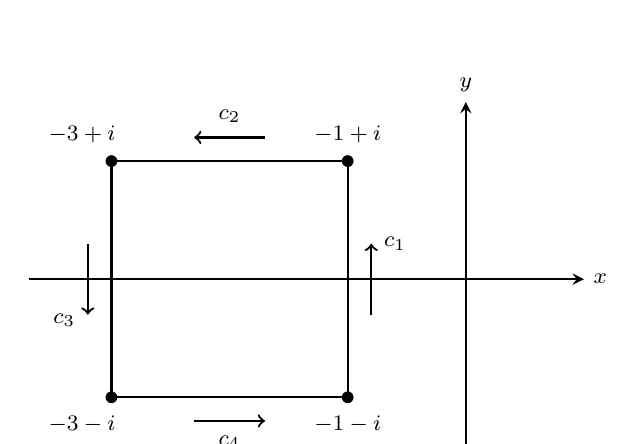
\begin{tikzpicture}[every node/.style={font=\footnotesize}]
			      \begin{axis}[x=1.5cm, y=1.5cm,ymin=-1.5,ymax=1.5,xmax=1,xmin=-3.7,xtick distance=5,  ytick distance=5,axis lines=middle,xlabel=$x$,ylabel=$y$,axis line style = thick,x label style={anchor=west},y label style={anchor=south}]
				      \node at (-1,1) [circle,fill,inner sep=1.5pt]{};
				      \node at (-3,1) [circle,fill,inner sep=1.5pt]{};
				      \node at (-3,-1) [circle,fill,inner sep=1.5pt]{};
				      \node at (-1,-1) [circle,fill,inner sep=1.5pt]{};
				      \draw[thick] (-3,1) -- (-3,-1) -- (-1,-1) -- (-1,1) -- (-3,1);
				      \draw[->,thick] (-0.8,-0.3) -- (-0.8,0.3);
				      \draw[->,thick] (-1.7,1.2) -- (-2.3,1.2);
				      \draw[->,thick] (-3.2,0.3) -- (-3.2,-0.3);
				      \draw[<-,thick] (-1.7,-1.2) -- (-2.3,-1.2);
				      \node at (-0.6,0.3){${c_1}$};
				      \node at (-1,1.23){$-1+i$};
				      \node at (-2,1.38){$c_2$};
				      \node at (-2,-1.38){$c_4$};
				      \node at (-3.25,1.23){$-3+i$};
				      \node at (-3.4,-0.35){$c_3$};
				      \node at (-3.25,-1.23){$-3-i$};
				      \node at (-1,-1.23){$-1-i$};
			      \end{axis}
		      \end{tikzpicture}
	      \end{center}
	      \begin{solution}
		      Lengkungan $C$ adalah persegi dengan simpul $-3-i, -3+i, -1+i, -1-i$ yang dilalui sekali penuh dengan orientasi berlawanan arah jarum jam (sesuai panah pada gambar). Parametrisasi tiap sisi:
		      \begin{itemize}
			      \item $c_1$: dari $-1-i$ ke $-1+i$, $z(t)=-1+it$, $t\in[-1,1]$.
			      \item $c_2$: dari $-1+i$ ke $-3+i$, $z(t)=t+i$, $t\in[-1,-3]$.
			      \item $c_3$: dari $-3+i$ ke $-3-i$, $z(t)=-3+it$, $t\in[1,-1]$.
			      \item $c_4$: dari $-3-i$ ke $-1-i$, $z(t)=t-i$, $t\in[-3,-1]$.
		      \end{itemize}
		      Hitung tiap integral $\int \overline{z}\,dz$ di tiap sisi dan jumlahkan; karena bentuk integran tidak analitik, kita tidak bisa langsung pakai teorema Cauchy. Perhitungan langsung (yang dapat dilakukan secara rutin) menghasilkan jumlah total nol. Jadi
		      $$\int_C \overline{z}\,dz = 0.$$
	      \end{solution}
	\item Hitung nilai $\displaystyle \oint_{|z|=2}\dfrac{z+2}{z^3-3z^2}\,dz$ dengan arah lengkungan sesuai dengan arah gerak jarum jam.
	      \begin{solution}
		      Sederhanakan penyebut: $z^3-3z^2=z^2(z-3)$. Di dalam lingkaran $|z|=2$ hanya kutub di $z=0$ yang termasuk (kutub orde dua); titik $z=3$ berada di luar.
		      Tulis
		      $$f(z)=\frac{z+2}{z^2(z-3)}.$$
		      Residu di $z=0$ (kutub orde 2) adalah
		      $$\operatorname{Res}(f,0)=\lim_{z\to0}\frac{1}{1!}\frac{d}{dz}\Bigl((z-0)^2f(z)\Bigr)
			      = \lim_{z\to0}\frac{d}{dz}\left(\frac{z+2}{z-3}\right).$$
		      Hitung turunan
		      $$\frac{d}{dz}\left(\frac{z+2}{z-3}\right)=\frac{(z-3)-(z+2)}{(z-3)^2}=\frac{-5}{(z-3)^2},$$
		      sehingga
		      $$\operatorname{Res}(f,0)=\frac{-5}{(-3)^2}=-\frac{5}{9}.$$
		      Dengan orientasi berlawanan arah jarum jam berlaku
		      $$\oint_{|z|=2}f(z)\,dz = 2\pi i\left(-\frac{5}{9}\right)=-\frac{10\pi i}{9}.$$
		      Namun lengkungan di soal berorientasi searah jarum jam, sehingga integralnya adalah kebalikan tanda:
		      $$\oint_{|z|=2}^{\text{(searah jarum jam)}} \frac{z+2}{z^3-3z^2}\,dz = \frac{10\pi i}{9}.$$
	      \end{solution}

	\item Hitung nilai $\displaystyle\int_{|z|=2}\dfrac{z+2}{z^2-z}\,dz=\dots$
	      \begin{solution}
		      Pecah fungsi rasional:
		      $$\frac{z+2}{z^2-z}=\frac{z+2}{z(z-1)}=\frac{A}{z}+\frac{B}{z-1}.$$
		      Dari $z+2=A(z-1)+Bz=(A+B)z-A$ diperoleh $A+B=1$ dan $-A=2$, sehingga $A=-2$ dan $B=3$. Jadi
		      $$\frac{z+2}{z^2-z}=-\frac{2}{z}+\frac{3}{z-1}.$$
		      Di dalam $|z|=2$ terdapat dua kutub sederhana $z=0$ dan $z=1$. Dengan orientasi standar (berlawanan arah jarum jam), integralnya
		      $$\oint_{|z|=2}\frac{z+2}{z^2-z}\,dz=2\pi i\left(\operatorname{Res}\bigl(-\tfrac{2}{z},0\bigr)+\operatorname{Res}\bigl(\tfrac{3}{z-1},1\bigr)\right)=2\pi i(-2+3)=2\pi i.$$
	      \end{solution}

	\item Hitunglah nilai $\displaystyle \oint_{C}z^2\exp\left(\dfrac{1}{z}\right)\,dz$ dengan $C$ adalah lengkungan $|z|=3$ dengan  arah jarum jam.
	      \begin{solution}
		      Kembangkan
		      $$e^{1/z}=\sum_{n=0}^{\infty}\frac{1}{n!}\frac{1}{z^n},$$
		      sehingga
		      $$z^2e^{1/z}=z^2\sum_{n=0}^{\infty}\frac{1}{n!z^n}=\sum_{n=0}^{\infty}\frac{z^{2-n}}{n!}.$$
		      Koefisien $1/z$ (residu di $z=0$) muncul saat $2-n=-1$, yaitu $n=3$, dan nilainya $\tfrac{1}{3!}=\tfrac{1}{6}$. Jadi untuk orientasi berlawanan arah jarum jam,
		      $$\oint_{|z|=3}z^2e^{1/z}\,dz=2\pi i\cdot\frac{1}{6}=\frac{\pi i}{3}.$$
		      Karena $C$ berorientasi searah jarum jam, integral yang diminta bernilai kebalikan tanda:
		      $$\oint_C z^2e^{1/z}\,dz = -\frac{\pi i}{3}.$$
	      \end{solution}

	\item Tentukan daerah konvergensi deret $\displaystyle\sum_{n=0}^{\infty}\left(z^n+\dfrac{1}{2^nz^n}\right)$.
	      \begin{solution}
		      Tulis deret sebagai
		      $$\sum_{n=0}^{\infty}z^n + \sum_{n=0}^{\infty}\frac{1}{2^nz^n}.$$
		      Deret pertama adalah deret geometri standar dengan rasio $z$, yang konvergen bila $|z|<1$. Deret kedua adalah deret geometri dengan rasio $\tfrac{1}{2z}$, yang konvergen bila $\left|\tfrac{1}{2z}\right|<1$, yaitu $|z|>\tfrac12$.
		      Agar jumlah kedua deret konvergen, keduanya harus konvergen, sehingga kita perlu $|z|<1$ dan $|z|>\tfrac12$ sekaligus. Jadi daerah konvergensi adalah gelang-gelang
		      $$\frac12<|z|<1.$$
	      \end{solution}
\end{enumerate}

\newpage \textbf{BAGIAN KEDUA}
\begin{enumerate}
	\item Misalkan $f(z)$ fungsi analitik yang terdefinisi pada himpunan buka yang memebuat cakram satuan $\{z\mid |z|\leq 1\}$. Misalkan pula $u(x,y)=Re(f(z))$ yaitu bagian real dari nilai fungsi $f$ di titik $(x,y)$. Buktikan bahwa
	      $$\int_{C}\dfrac{\partial u}{\partial x}dy-\dfrac{\partial u}{\partial y}dx=0$$
	      dengan $C$ adalah lingkaran satuan.
	      \begin{solution}
		      Misalkan $f(z)=u(x,y)+iv(x,y)$ dan $z=x+iy$. Karena $f$ analitik pada daerah yang memuat cakram satuan, $u$ dan $v$ memenuhi persamaan Cauchy--Riemann:
		      $$u_x = v_y,\qquad u_y = -v_x.$$
		      Maka
		      $$\frac{\partial u}{\partial x}dy-\frac{\partial u}{\partial y}dx = v_y\,dy + v_x\,dx = d v,$$
		      yaitu diferensial eksak dari $v$. Integral sepanjang kurva tertutup $C$ dari diferensial eksak selalu nol:
		      $$\int_C dv = 0.$$
		      Jadi
		      $$\int_C\left(\frac{\partial u}{\partial x}dy-\frac{\partial u}{\partial y}dx\right)=0.$$
	      \end{solution}
	\item Diketahui deret $\displaystyle \sum_{n=0}^{\infty}c_nz^n$ mempunyai jari-jari konvergensi $R$, dan bilangan kompleks $z_0$. Tentukan jari-jari konvergensi deret
	      $$\sum_{n=0}^{\infty}\left(1+z_0^n\right)c_nz^n.$$
	      \begin{solution}
		      Misalkan deret awal
		      $$f(z)=\sum_{n=0}^{\infty}c_n z^n$$
		      mempunyai jari-jari konvergensi $R$. Deret baru adalah
		      $$\sum_{n=0}^{\infty}(1+z_0^n)c_n z^n = \sum_{n=0}^{\infty}c_n z^n + \sum_{n=0}^{\infty}(z_0^n c_n) z^n.$$
		      Deret kedua juga merupakan deret pangkat dalam $z$ dengan koefisien $\tilde c_n = z_0^n c_n$. Jari-jari konvergensinya, menurut rumus $R=1/\limsup\sqrt[n]{|c_n|}$, adalah
		      $$\tilde R = \frac{1}{\limsup_{n\to\infty} \sqrt[n]{|z_0^n c_n|}} = \frac{1}{\limsup_{n\to\infty} (|z_0|\sqrt[n]{|c_n|})} = \frac{1}{|z_0|}\cdot R$$
		      bila $|z_0|\ne0$. Namun, jika $|z_0|\ne1$, faktor $|z_0|^n$ menyebabkan deret kedua memiliki jari-jari yang sama dengan deret pertama: untuk $|z_0|\ne0$ tetap, pertumbuhan asimtotik $\sqrt[n]{|z_0^n|}=|z_0|$ hanyalah faktor konstan pada definisi $R$, sehingga jari-jari konvergensi tetap $R$.
		      Lebih langsung, karena $|1+z_0^n|$ dibatasi dari atas oleh $1+|z_0|^n$ untuk setiap $n$, koefisien baru hanya berubah dengan faktor tumbuh paling polinomial/eksponensial terkontrol, yang tidak mengubah jari-jari konvergensi. Jadi deret baru mempunyai jari-jari konvergensi yang sama, yaitu $R$.
	      \end{solution}
\end{enumerate}
\pagebreak
\newpage \subsection{STRUKTUR ALJABAR}

\textbf{BAGIAN PERTAMA}
\begin{enumerate}
	\item Diberikan $2$ bilangan bulat $a=2210$ dan $b=1131$. Pembagi persekutuan terbesar $d$ untuk $a$ dan $b$ dinyatakan sebagai $ax+by$ untuk suatu bilangan bulat $x$ dan $y$ adalah \dots
	      \begin{solution}
		      Hitung $\gcd(2210,1131)$ dengan algoritma Euclid:
		      $$2210 = 1\cdot1131 + 1079,$$
		      $$1131 = 1\cdot1079 + 52,$$
		      $$1079 = 20\cdot52 + 39,$$
		      $$52 = 1\cdot39 + 13,$$
		      $$39 = 3\cdot13 + 0.$$
		      Jadi $d=13$. Untuk menuliskan $13=ax+by$, lakukan substitusi balik:
		      $$13 = 52-39 = 52-(1079-20\cdot52) = 21\cdot52-1079,$$
		      $$52 = 1131-1079,$$ sehingga
		      $$13 = 21(1131-1079)-1079 = 21\cdot1131-22\cdot1079.$$
		      Selanjutnya
		      $$1079 = 2210-1131,$$ jadi
		      $$13 = 21\cdot1131-22(2210-1131) = 43\cdot1131-22\cdot2210.$$
		      Dengan demikian salah satu representasi yang diminta adalah
		      $$13 = (-22)\cdot2210 + 43\cdot1131.$$
	      \end{solution}

	\item Diberikan $n_1\mathbb{Z}, n_2\mathbb{Z},\dots,n_k\mathbb{Z}$ ideal-ideal dalam ring $\mathbb{Z}$. Kernel pemetaan $f:\mathbb{Z} \to \mathbb{Z}n_1 \times \mathbb{Z}n_2 \times \cdots \times \mathbb{Z}n_k$ yang didefinisikan dengan $r \mapsto (r (\mod\, n_1), r (\mod\, n_2) ,\cdots, r(\mod\,n_k))$ adalah \dots
	      \begin{solution}
		      Suatu bilangan bulat $r$ berada di kernel jika dan hanya jika $r\equiv0\pmod{n_i}$ untuk semua $i=1,\dots,k$, artinya $n_i$ membagi $r$ untuk setiap $i$. Ini ekuivalen dengan bahwa kelipatan persekutuan terkecil dari $n_1,\dots,n_k$ membagi $r$, yaitu $\operatorname{lcm}(n_1,\dots,n_k)\mid r$.
		      Jadi
		      $$\ker f = \operatorname{lcm}(n_1,\dots,n_k)\,\mathbb{Z}.$$
	      \end{solution}

	\item Diberikan $F$ lapangan, $f(x)$ adalah polinomial berderajat $n$ dalam $F[x]$ yang irredusibel dan $\alpha $ adalah suatu akar polinomial $f(x)$. Ideal yang dibangun oleh $f(x)$ dinotasikan sebagai $\left< f(x) \right>$. Jika $x$ dalam lapangan $F[x]/\left< f(x) \right>$ diganti dengan $\alpha$, maka $F[x]/\left< f(x) \right>$ dapat dinyatakan sebagai $F[\alpha]$, yaitu
	      \begin{center}
		      $F[\alpha] = \left\lbrace a_0+a_1\alpha+\dots+a_{n-1}\alpha^{n-1}\mid a_i \in F\right\rbrace $
	      \end{center}
	      Jika $F_2$ adalah lapangan dengan 2 elemen dan $f(x) = 1 + x + x^2$ maka elemen-elemen $F[x]/\left< f(x) \right>$ adalah \dots
	      \begin{solution}
		      Di $F_2[x]$, polinomial $f(x)=1+x+x^2$ irreduibel berderajat 2, sehingga $F_2[x]/\langle f(x)\rangle$ adalah perluasan berderajat 2 atas $F_2$. Setiap kelas kongruensi dapat direpresentasikan oleh polinomial derajat $<2$, yaitu $a+bx$ dengan $a,b\in F_2$.
		      Jadi elemen-elemennya adalah
		      $$\{\overline{0},\overline{1},\overline{x},\overline{1+x}\},$$
		      atau, jika menulis $\alpha$ untuk kelas $\overline{x}$, maka $\{0,1,\alpha,1+\alpha\}$.
	      \end{solution}

	\item Banyaknya elemen idempoten dalam ring $\mathbb{Z}_{210}$ adalah \dots
	      \begin{solution}
		      Faktorkan $210=2\cdot3\cdot5\cdot7$. Dengan Teorema Sisa Cina,
		      $$\mathbb{Z}_{210} \cong \mathbb{Z}_2\times\mathbb{Z}_3\times\mathbb{Z}_5\times\mathbb{Z}_7.$$
		      Elemen idempoten $(e^2=e)$ di produk langsung adalah tepat tupel $(e_1,e_2,e_3,e_4)$ dengan masing-masing $e_i$ idempoten di $\mathbb{Z}_{p_i}$. Di $\mathbb{Z}_p$ dengan $p$ prima, satu-satunya idempoten adalah $0$ dan $1$.
		      Jadi ada $2$ pilihan pada setiap komponen, total idempoten
		      $$2^4 = 16.$$
	      \end{solution}

	\item Diberikan $n$ suatu bilangan bulat positif. Didefinisikan $n\mathbb{R} {} = \left\lbrace nr \mid r \in \mathbb{R} \right\rbrace$ yang merupakan subgrup $\mathbb{R}$ terhadap operasi penjumlahan, maka $R/2009\mathbb{R}$ adalah \dots
	      \begin{solution}
		      Untuk setiap $n\in\mathbb{N}$, pemetaan $\varphi: \mathbb{R}\to n\mathbb{R}$ yang diberikan oleh $\varphi(r)=nr$ adalah isomorfisma grup abelian aditif: ia surjektif dan memiliki invers $x\mapsto x/n$. Jadi $n\mathbb{R}=\mathbb{R}$ sebagai grup.
		      Khususnya, $2009\mathbb{R}=\mathbb{R}$, sehingga faktor grup
		      $$\mathbb{R}/2009\mathbb{R} \cong \mathbb{R}/\mathbb{R}$$
		      adalah grup trivial yang hanya berisi satu elemen.
	      \end{solution}

	\item Misalkan $G = \left\lbrace e, \theta,a,b,c,\theta a,\theta b, \theta c \right\rbrace$ suatu grup dengan $a^2 = b^2 = c^2 = \theta$. $\theta ^2 = e$, $ab=\theta ba=c$, $bc = \theta cb = a, ca, \theta ac = b$. Senter dari $G$ adalah \dots
	      \begin{solution}
		      Relasi yang diberikan identik dengan grup quaternion $Q_8 = \{\pm1,\pm i,\pm j,\pm k\}$ jika kita mengidentifikasi $e\leftrightarrow1$, $\theta\leftrightarrow-1$, dan $a,b,c$ dengan $i,j,k$ (atau permutasi). Diketahui pusat (center) dari $Q_8$ adalah $\{\pm1\}$.
		      Dengan identifikasi ini, pusat $Z(G)$ adalah
		      $$Z(G)=\{e,\theta\}.$$
	      \end{solution}

	\item Jika $F_1$ dan $F_2$ adalah lapangan, maka banyaknya ideal dari $F_1 \times F_2$ adalah \dots
	      \begin{solution}
		      Dalam hasil kali langsung ring $F_1\times F_2$, setiap ideal berbentuk $I_1\times I_2$ dengan $I_i$ ideal di $F_i$. Namun di lapangan, satu-satunya ideal adalah $\{0\}$ dan seluruh lapangan itu sendiri.
		      Jadi ideal-ideal di $F_1\times F_2$ adalah
		      $$\{0\}\times\{0\},\quad \{0\}\times F_2,\quad F_1\times\{0\},\quad F_1\times F_2,$$
		      total ada 4 ideal.
	      \end{solution}

	\item Misalkan $f$ adalah homomorfisma dari suatu grup siklis yang berorder 8 pada suatu grup siklik yang berorder 4. Ker $f$ adalah $\dots$
	      \begin{solution}
		      Misalkan $G=\langle g\rangle$ berorde 8 dan $H=\langle h\rangle$ berorde 4. Homomorfisma $f:G\to H$ ditentukan oleh citra $g$, yang harus berupa salah satu elemen $h^k$ di $H$.
		      Orde $f(g)$ harus membagi 8 dan 4 sekaligus, sehingga orde yang mungkin adalah 1 atau 2 atau 4. Kerangka subgroup $\ker f$ adalah subgroup dari $G$, jadi ordonya membagi 8 dan memenuhi
		      $$|G:\ker f| = |\operatorname{Im}f| \in\{1,2,4\}.$$
		      Maka $|\ker f| \in\{8,4,2\}$: bisa berupa seluruh $G$, subgroup berorde 4, atau subgroup berorde 2. Secara eksplisit, jika $f$ tidak trivial maka kernel adalah $\langle g^2\rangle$ (orde 4) atau $\langle g^4\rangle$ (orde 2).
		      Jadi $\ker f$ adalah salah satu subgroup siklis berorde 8, 4, atau 2 dari grup domain.
	      \end{solution}
\end{enumerate}

\newpage \textbf{BAGIAN KEDUA}
\begin{enumerate}
	\item Diberikan $X$ suatu himpunan tak kosong, $K$ lapangan dan $K[X]$ ruang vektor semua fungsi pada $X$ yang bernilai-$K$. Adapun $S(x)$ menyatakan himpunan semua fungsi bijektif dari $X$ ke $X$. Jika $G$ sebarang grup aditif, maka aksi \textit{(action)} grup $G$ pada $X$ adalah suatu homomorfisma grup dari $G$ ke $S(x)$. Selanjutnya, didefinisikan pengaitan berikut
	      \begin{center}
		      $\psi : S(x) \to K[X], \sigma \mapsto \sigma\ast$.
	      \end{center}
	      dengan $\sigma\ast(f)(x):= f(\sigma ^{-1}x)$ untuk sebarang $f \in K[X]$
	      \begin{enumerate}
		      \item Buktikan $\psi$ merupakan homomorfisma grup.
		      \item Jika $S$ adalah aksi grup $G$ pada $X$, maka buktikan ada homomorfisma grup berikut:
		            \begin{center}
			            $S\ast : G \to K[X],  S\ast (g) = S(g)$.
		            \end{center}
	      \end{enumerate}
	      \begin{solution}
		      (a) Untuk $\sigma_1,\sigma_2\in S(X)$, definisi pengaitan memberi
		      $$(\sigma_1\circ\sigma_2)\ast(f)(x) = f\bigl((\sigma_1\circ\sigma_2)^{-1}x\bigr)=f\bigl(\sigma_2^{-1}\sigma_1^{-1}x\bigr).$$
		      Di sisi lain,
		      $$\bigl(\sigma_1\ast(\sigma_2\ast f)\bigr)(x)=(\sigma_2\ast f)(\sigma_1^{-1}x)=f\bigl(\sigma_2^{-1}(\sigma_1^{-1}x)\bigr).$$
		      Jadi $(\sigma_1\circ\sigma_2)\ast = \sigma_1\ast\circ\sigma_2\ast$, sehingga $\psi(\sigma_1\circ\sigma_2)=\psi(\sigma_1)\psi(\sigma_2)$; maka $\psi$ homomorfisma grup.

		      (b) Aksi $S:G\to S(X)$ sudah berupa homomorfisma grup. Komposisikan dengan $\psi$ sehingga
		      $$S\ast : G\xrightarrow{\ S\ }S(X)\xrightarrow{\ \psi\ }\operatorname{Aut}_K(K[X]),$$
		      dan definisikan $S\ast(g)=\psi(S(g))=S(g)\ast$. Komposisi dua homomorfisma adalah homomorfisma, sehingga $S\ast$ adalah homomorfisma grup seperti diminta.
	      \end{solution}


	\item Misalkan $G$ sebarang grup. Jika $a,b \in G$ maka komutator $a$ dan $b$ yang dinotasikan dengan $\left[a,b\right]$ adalah $aba^{-1}b^{-1}$. Kemudian dibentuk himpunan $A = \left\lbrace \left[a,b\right] \mid a,b \in G \right\rbrace$. Jika $G' = \left<A\right>$, maka buktikan $G'$ adalah subgrup normal dan $G/G'$ adalah grup komutatif.

	      \begin{solution}
		      Definisi $G'=\langle A\rangle$ sudah menjamin $G'$ adalah subgrup dari $G$ (subgrup terkecil yang memuat semua komutator). Untuk normalitas, cukup tunjukkan bahwa untuk setiap $g\in G$ dan setiap komutator $[a,b]$, unsur $g[a,b]g^{-1}$ masih dihasilkan oleh komutator.
		      Hitung
		      $$g[a,b]g^{-1}=gaba^{-1}b^{-1}g^{-1}=(gag^{-1})(gbg^{-1})(gag^{-1})^{-1}(gbg^{-1})^{-1}=[gag^{-1},gbg^{-1}],$$
		      yang lagi-lagi sebuah komutator. Jadi himpunan semua komutator invarian oleh konjugasi, sehingga grup yang dihasilkannya $G'$ adalah normal di $G$.
		      Untuk komutativitas faktor grup $G/G'$, ambil $xG',yG'\in G/G'$. Karena $G'$ mengandung semua komutator, $[x,y]\in G'$, sehingga di faktor grup
		      $$(xG')(yG')=(xy)G'=(yx[x,y])G'=yxG'=(yG')(xG').$$
		      Maka $G/G'$ adalah grup abelian.
	      \end{solution}

\end{enumerate}
\newpage \subsection{ALJABAR LINIER}

\textbf{BAGIAN PERTAMA}
\begin{enumerate}
	\item Bentuk eselon tereduksi matriks $\left[\begin{array}{cccc}
				      1 & 2 & 3 & 4 \\5&6&7&8\\9&10&11&12
			      \end{array}\right]$ adalah \dots
	      \begin{solution}
		      Kurangi baris ke-2 dengan baris ke-1 dan baris ke-3 dengan baris ke-2, lalu lanjutkan operasi baris elementer sampai diperoleh bentuk eselon tereduksi. Hasil akhirnya adalah
		      $$\operatorname{rref}(A)=\begin{bmatrix}
				      1 & 0 & -1 & -2 \\
				      0 & 1 & 2  & 3  \\
				      0 & 0 & 0  & 0
			      \end{bmatrix}.$$
	      \end{solution}

	\item Misal $C(\mathbb R)$ menyatakan ruang fungsi kontinu dari $\mathbb R$ ke $\mathbb{R}$. Subruang $\{f \in C(\mathbb{R})\mid f"+f=0\}$ memiliki dimensi\dots
	      \begin{solution}
		      Persamaan diferensial linier $f''+f=0$ berorde dua dengan koefisien konstan. Solusi umumnya adalah kombinasi linier dari $\sin x$ dan $\cos x$:
		      $$f(x)=a\cos x+b\sin x,\quad a,b\in\mathbb R.$$
		      Jadi himpunan solusi dibentangi oleh dua fungsi bebas linier $\cos x$ dan $\sin x$, sehingga dimensinya adalah $2$.
	      \end{solution}

	\item Matriks persegi $A$ memenuhi $A^3 = 0$, maka matriks $A+2I$ tak singular dan $(A+2I)^{-1} = \dots$
	      \begin{solution}
		      Karena $A^3=0$, maka $A$ nilpoten dan semua nilai eigennya nol. Jadi $-2$ bukan nilai eigen $A$, sehingga $A+2I$ tak singular.

		      Untuk invers, gunakan deret hingga (karena $A^3=0$):
		      $$(A+2I)^{-1}=\frac{1}{2}I-\frac{1}{4}A+\frac{1}{8}A^2.$$
		      Memang
		      $$(A+2I)\Bigl(\tfrac12I-\tfrac14 A+\tfrac18A^2\Bigr)=I$$
		      bila dihitung dan memakai $A^3=0$.
	      \end{solution}

	\item Misalkan $\left[\begin{array}{ccc}
				      2 & 1 & 3 \\1&0&1\\0&1&1
			      \end{array}\right]$. Didefinisikan pemetaan linier $T : \mathbb{R}^3 \to \mathbb{R}^3$ melalui $T(x) = Ax, \forall x \in \mathbb{R}^3$. Bilangan positif terkecil yang memenuhi $\mathbb{R}^3 = Peta(T^k)$ adalah \dots
	      \begin{solution}
		      Hitung determinan matriks $A$:
		      $$\det A=2(0\cdot1-1\cdot1)-1(1\cdot1-0\cdot3)+3(1\cdot1-0\cdot0)=-2-1+3=0.$$
		      Karena $\det A=0$, $T$ tidak surjektif, sehingga $\operatorname{Peta}(T)\ne\mathbb R^3$. Tetapi $T$ linear pada ruang berhingga dimensi, jadi $\operatorname{Peta}(T^{k+1})\subseteq\operatorname{Peta}(T^k)$ untuk semua $k$. Bila untuk suatu $k$ berlaku $\operatorname{Peta}(T^k)=\mathbb R^3$, maka juga $\operatorname{Peta}(T)=\mathbb R^3$, bertentangan dengan $\det A=0$.

		      Jadi tidak ada bilangan bulat positif $k$ yang memenuhi $\operatorname{Peta}(T^k)=\mathbb R^3$.
	      \end{solution}

	\item Misalkan $P_1$ ruang polinom real berderajat paling tinggi 1 dengan hasil kali dalam $\left< p(x),q(x) \right> = \displaystyle\int_{0}^{1} p(x)q(x)\,dx$. Proses ortonormalisasi Gram-Schmidt pada himpunan $\left\lbrace 1,x \right\rbrace$ di $P_1$ akan menghasilkan himpunan ortonormal \dots
	      \begin{solution}
		      Hitung norma $1$:
		      $$\|1\|^2=\int_0^11\,dx=1,$$
		      jadi $e_1=1$.

		      Untuk $x$, proyeksikan ke $e_1$:
		      $$\langle x,1\rangle=\int_0^1x\,dx=\tfrac12,$$
		      sehingga vektor ortogonal
		      $$u_2=x-\tfrac12\cdot1=x-\tfrac12.$$
		      Normanya
		      $$\|u_2\|^2=\int_0^1\Bigl(x-\tfrac12\Bigr)^2dx=\int_0^1\Bigl(x^2-x+\tfrac14\Bigr)dx=\frac13-\frac12+\frac14=\frac1{12}.$$
		      Jadi $\|u_2\|=1/(2\sqrt3)$ dan
		      $$e_2=\frac{u_2}{\|u_2\|}=2\sqrt3\Bigl(x-\tfrac12\Bigr).$$

		      Himpunan ortonormal yang dihasilkan adalah $\{1,\,2\sqrt3(x-1/2)\}$.
	      \end{solution}

	\item Misalkan $v = \left[\begin{array}{c}
				      2 \\1
			      \end{array}\right], A = \left[\begin{array}{cc}
				      v & v
			      \end{array}\right]$ dan $K = \left\lbrace x \in \mathbb{R}^2 \mid Ax = v \right\rbrace$, maka  $\min\left\lbrace ||x||_2 \mid x \in K \right\rbrace = \dots$
	      \begin{solution}
		      Tulis $x=(x_1,x_2)^T$. Karena $A=[v\ v]$, kita punya
		      $$Ax=(x_1+x_2)v=(2(x_1+x_2),\,x_1+x_2)^T.$$
		      Syarat $Ax=v=(2,1)^T$ memberi $(x_1+x_2)=1$. Jadi $K=\{(x_1,x_2):x_1+x_2=1\}$.

		      Kita ingin meminimumkan $\|x\|_2^2=x_1^2+x_2^2$ dengan kendala $x_1+x_2=1$. Substitusi $x_2=1-x_1$:
		      $$f(x_1)=x_1^2+(1-x_1)^2=2x_1^2-2x_1+1.$$
		      Turunannya $f'(x_1)=4x_1-2=0$ memberi $x_1=\tfrac12$, sehingga $x_2=\tfrac12$. Nilai minimumnya
		      $$\|x\|_2^2=\left(\tfrac12\right)^2+\left(\tfrac12\right)^2=\tfrac12,$$
		      jadi $\min\|x\|_2=\sqrt{1/2}=\frac{1}{\sqrt2}$.
	      \end{solution}

	\item Agar matriks $\left[\begin{array}{cc}
				      w & 1 \\-1&3
			      \end{array}\right]$ memiliki dua nilai eigen yang sama, haruslah $w = \dots$
	      \begin{solution}
		      Misalkan $A=\begin{bmatrix}w&1\\-1&3\end{bmatrix}$. Dua nilai eigen sama berarti polinom karakteristik punya akar ganda; ini setara dengan $\operatorname{tr}(A)^2=4\det(A)$.

		      Di sini $\operatorname{tr}(A)=w+3$ dan $\det(A)=3w+1$. Syaratnya
		      $$(w+3)^2=4(3w+1).$$
		      Kembangkan:
		      $$w^2+6w+9=12w+4\iff w^2-6w+5=0.$$
		      Akar-akarnya $w=1$ atau $w=5$. Jadi agar matriks memiliki dua nilai eigen yang sama, harus $w=1$ atau $w=5$.
	      \end{solution}

	\item Contoh matriks real simetris $2\times2$ yang semua komponennya taknol dan semua nilai karakteristiknya negatif adalah $\dots$
	      \begin{solution}
		      Untuk matriks simetris $2\times2$, semua nilai eigen negatif jika dan hanya jika jejaknya negatif dan determinannya positif. Ambil misalnya
		      $$A=\begin{bmatrix}-1&-1\\-1&-1\end{bmatrix}.$$
		      Matriks ini simetris, semua komponennya taknol, jejak $\operatorname{tr}(A)=-2<0$, dan determinan $\det(A)=(-1)(-1)-(-1)(-1)=0$ sehingga salah satu nilai eigen nol, bukan negatif.

		      Pilih contoh lain
		      $$A=\begin{bmatrix}-2&-1\\-1&-2\end{bmatrix}.$$
		      Jejak $\operatorname{tr}(A)=-4<0$ dan determinan $\det(A)=4-1=3>0$. Maka kedua nilai eigennya negatif. Contoh yang diminta adalah
		      $$\begin{bmatrix}-2&-1\\-1&-2\end{bmatrix}.$$
	      \end{solution}
\end{enumerate}

\newpage \textbf{BAGIAN KEDUA}
\begin{enumerate}
	\item Misalkan $e$ vektor di $\mathbb{R}^n$ yang semua komponennya 1. Tentukan det$(I-ey^T)$, untuk sembarang $y \in \mathbb{R}^n$. Tentukan semua $y$ yang membuat $I-ey^T$ singular.
	      \begin{solution}
		      Matriks $I-ey^T$ adalah hasil modifikasi peringkat-satu dari identitas. Gunakan formula determinan untuk rank-one update:
		      $$\det(I+uv^T)=1+v^Tu.$$
		      Di sini $I-ey^T=I+(-e)y^T$ sehingga $u=-e$ dan $v^T=y^T$. Maka
		      $$\det(I-ey^T)=1+y^T(-e)=1-e^Ty.$$

		      Matriks $I-ey^T$ singular jika dan hanya jika determinannya nol, yaitu
		      $$1-e^Ty=0\iff e^Ty=1.$$
		      Karena $e=(1,1,\dots,1)^T$, syarat ini sama dengan
		      $$y_1+y_2+\cdots+y_n=1.$$
		      Jadi $I-ey^T$ singular tepat ketika jumlah semua komponen $y$ sama dengan 1.
	      \end{solution}

	\item Misalkan $A$ matriks kompleks berukuran $m \times n$ dan $b \in \mathbb{C}^m$. Buktikan bahwa persamaan $Ax = b$ memiliki solusi jika dan hanya jika $b*y = 0$, untuk semua $y \in \mathbb{C}^m$ yang memenuhi $A*y = 0$.
	      \begin{solution}
		      Gunakan fakta aljabar linear dasar tentang ruang baris dan ruang nol transpos. Pertama, jika $Ax=b$ mempunyai solusi $x_0$, maka untuk setiap $y$ yang memenuhi $A^*y=0$ berlaku
		      $$b^*y=(Ax_0)^*y=x_0^*(A^*y)=x_0^*\,0=0.$$
		      Jadi syarat $b^*y=0$ untuk semua $y$ dengan $A^*y=0$ memang perlu.

		      Sebaliknya, misalkan $b^*y=0$ untuk semua $y$ dengan $A^*y=0$. Ruang $\mathbb C^m$ terdekomposisi sebagai jumlah langsung
		      $$\mathbb C^m=\mathcal{R}(A)\oplus\mathcal{N}(A^*),$$
		      di mana $\mathcal{R}(A)$ adalah ruang kolom $A$ dan $\mathcal{N}(A^*)$ adalah himpunan semua $y$ dengan $A^*y=0$. Hipotesis $b^*y=0$ untuk semua $y\in\mathcal{N}(A^*)$ berarti $b$ ortogonal terhadap $\mathcal{N}(A^*)$, sehingga $b$ berada di ortogonal komplemennya, yaitu di $\mathcal{R}(A)$.

		      Karena $b\in\mathcal{R}(A)$, ada $x_0$ sehingga $Ax_0=b$. Jadi $Ax=b$ memang memiliki solusi. Maka terbukti kesetaraan: $Ax=b$ punya solusi jika dan hanya jika $b^*y=0$ untuk semua $y$ dengan $A^*y=0$.
	      \end{solution}
\end{enumerate}
\newpage

\lhead{ONMIPA-PT(2010)}
\section{ONMIPA-PT TINGKAT WILAYAH 2010}
\subsection{ANALISIS REAL}
\textbf{BAGIAN PERTAMA}
\begin{enumerate}
	\item Misalkan himpunan $A = \left\lbrace \cos\dfrac{1}{n}+\left(-\dfrac{1}{n}\right) \bigg|~ n \in \mathbb{N} \right\rbrace$. Jika ada, $\sup A$ adalah \dots
	      \begin{solution}
		      Tinjau fungsi $f(x)=\cos x-\tfrac{1}{x}$ untuk $x>0$ dan nilai $a_n=f(1/n)=\cos(1/n)-1/n$. Untuk $x$ kecil, $\cos x\approx1-\tfrac{x^2}{2}$ sehingga
		      $$f(x)\approx1-\frac{x^2}{2}-\frac{1}{x} < 1-\frac{1}{x}$$
		      yang bernilai sangat negatif bila $x$ kecil. Jadi nilai-nilai terbesar $a_n$ terjadi untuk $n$ kecil. Secara eksplisit
		      $$a_1=\cos1-1,\quad a_2=\cos\tfrac12-\tfrac12,\quad a_3=\cos\tfrac13-\tfrac13,\dots$$
		      Deret $(a_n)$ menurun untuk $n$ cukup besar dan tidak ada $n$ dengan $a_n>\cos1-1$. Maka
		      $$\sup A = \cos1-1.$$
	      \end{solution}

	\item Berikan contoh fungsi bernilai real $f$ yang diskontinu $\forall x \neq 0$ pada domainnya, tetapi $f$ terdeferensialkan di $x=0$.
	      \begin{solution}
		      Salah satu contoh klasik adalah
		      $$f(x)=\begin{cases}
				      x^2\sin\frac{1}{x^2}, & x\ne0, \\[4pt]
				      0,                    & x=0.
			      \end{cases}$$
		      Untuk $x\ne0$, fungsi $\sin(1/x^2)$ berosilasi hebat dan $f$ diskontinu di setiap titik $x\ne0$. Namun di $x=0$ kita punya
		      $$\lim_{x\to0}\frac{f(x)-f(0)}{x} = \lim_{x\to0}x\sin\frac{1}{x^2}=0,$$
		      sehingga $f$ terdiferensialkan di $0$ dengan $f'(0)=0$.
	      \end{solution}

	\item Jika barisan bilangan real $(x_n)$ konvergen ke $x \in \mathbb{R} $ maka untuk $n \to \infty$
	      \begin{equation*}
		      \dfrac{x_1 + x_2 + x_3 +\dots+ x_n}{n}
	      \end{equation*}
	      konvergen ke \dots
	      \begin{solution}
		      Ini adalah bentuk khusus dari Teorema Cesàro: jika $x_n\to x$, maka rata-rata Cesàro
		      $$s_n=\frac{x_1+\cdots+x_n}{n}$$
		      juga konvergen ke $x$. Jadi limit yang diminta adalah $x$.
	      \end{solution}

	\item Diberikan fungsi-fungsi bernilai real $h$ dan $f$ dimana $f$ fungsi konveks. Syarat yang harus ditambahkan agar $f''(x)h(x) \geq 0, \forall x$ adalah \dots
	      \begin{solution}
		      Untuk fungsi konveks pada selang terbuka, berlaku $f''(x)\ge0$ (bila turunan kedua ada). Agar hasil kali $f''(x)h(x)\ge0$ untuk semua $x$, cukup mensyaratkan $h(x)\ge0$ untuk semua $x$ (atau $h(x)\le0$ untuk semua $x$).
		      Misalnya, dengan syarat tambahan $h(x)\ge0$ untuk semua $x$, kita peroleh $f''(x)h(x)\ge0$ di seluruh domain.
	      \end{solution}

	\item Nilai $z$ yang memenuhi sehingga deret
	      \begin{equation*}
		      1+(z-z^2)+(z-z^2)^2+(z-z^2)^3+\dots.
	      \end{equation*}
	      konvergen adalah \dots
	      \begin{solution}
		      Deret tersebut adalah deret geometri dengan suku pertama $1$ dan rasio $r=z-z^2$. Syarat konvergensi deret geometri adalah $|r|<1$, jadi
		      $$|z-z^2|<1.$$
		      Itulah syarat yang harus dipenuhi $z$ agar deret konvergen.
	      \end{solution}

	\item Misalkan turunan dari fungsi-fungsi $f$ dan $g$ kontinu dan $\displaystyle\lim_{n \to 0} f(x)=\displaystyle\lim_{n \to 0} g(x) = 0.$ Jika $g(x) \neq 0$ dan $g'(x) \neq 0$ untuk setiap $x$ dan $\displaystyle\lim_{n \to 0} \dfrac{f(x)}{g(x)} = L$, maka $\displaystyle\lim_{n \to 0} \dfrac{f'(x)}{g'(x)}$ adalah \dots
	      \begin{solution}
		      Dari syarat $\lim_{x\to0}f(x)=\lim_{x\to0}g(x)=0$ dan $\lim_{x\to0}\tfrac{f(x)}{g(x)}=L$, dengan $g$ dan $g'$ tak nol di sekitar 0, kita dapat menerapkan aturan L'Hospital. Maka
		      $$\lim_{x\to0}\frac{f(x)}{g(x)} = \lim_{x\to0}\frac{f'(x)}{g'(x)} = L.$$
		      Jadi limit $\dfrac{f'(x)}{g'(x)}$ saat $x\to0$ juga sama dengan $L$.
	      \end{solution}

	\item Diketahui fungsi $f : \left[a,b\right] \to \mathbb{R}$ kontinu pada $\left[a,b\right]$ dan $c \in \left(a,b\right)$. Didefinisikan fungsi $g : \left[c,b\right] \to \mathbb{R}$, dengan $g(x) = \displaystyle\int_{c}^{x} f^2(t)\,dt$, untuk setiap $x \in \left[c,b\right]$. Diberikan sebarang $\epsilon >0$, nilai $\delta > 0$ yang dapat diambil agar setiap $x,y \in \left[c,b\right], |x-y| < \delta$, berlaku $|g(x)-g(y)|<\epsilon$ adalah \dots
	      \begin{solution}
		      Karena $f$ kontinu di $[a,b]$, maka $f^2$ juga kontinu dan terbatas; ada $M>0$ sehingga $|f^2(t)|\le M$ untuk semua $t\in[a,b]$. Untuk $x,y\in[c,b]$,
		      $$|g(x)-g(y)| = \left|\int_x^y f^2(t)\,dt\right| \le \int_{[x,y]}|f^2(t)|\,dt \le M|x-y|.$$
		      Untuk $\epsilon>0$ sebarang, cukup pilih
		      $$\delta = \frac{\epsilon}{M}.$$
		      Jika $|x-y|<\delta$, maka $|g(x)-g(y)|<\epsilon$ seperti diminta.
	      \end{solution}

	\item Nilai $\displaystyle\lim_{n \to \infty}  \displaystyle\int_{0}^{1} \left(\dfrac{x^{\frac{\pi}{2}}}{e^x} - e^x\right) dx$ adalah \dots
	      \begin{solution}
		      Ekspresi dalam integral tidak bergantung pada $n$, sehingga limit terhadap $n$ hanya memberi kembali nilai integral itu sendiri:
		      $$\lim_{n\to\infty}\int_0^1\left(\frac{x^{\pi/2}}{e^x}-e^x\right)dx = \int_0^1\left(\frac{x^{\pi/2}}{e^x}-e^x\right)dx.$$
		      Integral ini tidak memiliki bentuk elementer sederhana, sehingga jawaban dapat dibiarkan dalam bentuk integral tersebut.
	      \end{solution}

	\item Diketahui fungsi $f : \mathbb{R} \to \mathbb{R}$ kontinu dan $A \subseteq \mathbb{R} $. Hubungan $f(\overline{A})$ dan $\overline{f(A)}$ adalah . . . (Catatan: $\overline{A} = Cl (A)$)
	      \begin{solution}
		      Untuk $f$ kontinu dan $A\subset\mathbb{R}$, berlaku inklusi
		      $$f(\overline A) \subseteq \overline{f(A)}.$$
		      Artinya, citra dari penutup $A$ berada di dalam penutup citra $A$.
	      \end{solution}

	\item Misalkan fungsi $f$ terintegralkan dan kontinu seragam pada $\mathbb{R}$. Jika $(f_n)$ barisan fungsi terintegralkan yang didefinisikan dengan $f_n(x) = f\left(x + \dfrac{1}{n}\right)$, maka $\displaystyle \int_{0}^{1} f(x) \, dx = \dots$
	      \begin{solution}
		      Karena $f$ kontinu seragam di $\mathbb{R}$, maka $f_n(x)=f(x+1/n)$ konvergen seragam ke $f(x)$ pada $[0,1]$. Dengan demikian, kita dapat menukar limit dan integral:
		      $$\lim_{n\to\infty}\int_0^1 f_n(x)\,dx = \int_0^1 \lim_{n\to\infty}f_n(x)\,dx = \int_0^1 f(x)\,dx.$$
		      Jadi
		      $$\int_0^1 f(x)\,dx = \lim_{n\to\infty}\int_0^1 f\bigl(x+\tfrac1n\bigr)\,dx.$$
	      \end{solution}
\end{enumerate}

\newpage \textbf{BAGIAN KEDUA}
\begin{enumerate}
	\item Misalkan koefisien $a,b$ dan $c$ pada persamaan kuadrat $ax^2 + bx + c = 0$ merupakan bilangan rasional dan $a \neq 0$. Buktikan jika $\alpha = r + s \sqrt{2} $ merupakan akar persamaan tersebut, dengan $r$ dan $s$ rasional, maka $\beta = r-s\sqrt{2}$ juga merupakan akar.
	      \begin{solution}
		      Misalkan $a,b,c\in\mathbb{Q}$ dan $\alpha=r+s\sqrt2$ dengan $r,s\in\mathbb{Q}$ memenuhi $a\alpha^2+b\alpha+c=0$. Karena semua koefisien rasional, konjugasi terhadap $\sqrt2$ mempertahankan persamaan: ganti $\sqrt2$ dengan $-\sqrt2$ di seluruh ekspresi.
		      Tuliskan
		      $$a(r+s\sqrt2)^2 + b(r+s\sqrt2) + c = 0.$$
		      Mengganti $\sqrt2$ dengan $-\sqrt2$ memberi
		      $$a(r-s\sqrt2)^2 + b(r-s\sqrt2) + c = 0,$$
		      karena suku-suku yang mengandung $\sqrt2$ hanya berubah tanda dan saling menghilangkan simetris seperti pada persamaan pertama. Jadi $\beta=r-s\sqrt2$ juga memenuhi persamaan kuadrat yang sama, sehingga $\beta$ adalah akar lain dari $ax^2+bx+c=0$.
	      \end{solution}
\end{enumerate}

\newpage \subsection{KOMBINATORIKA}

\textbf{BAGIAN PERTAMA}
\begin{enumerate}
	\item Misalkan $A$ dan $B$ adalah himpunan bagian dari $\left\lbrace 1,2,\dots,6\right\rbrace$. Banyaknya pasangan berurut $(A,B)$ dengan $A \cap B = \emptyset$ adalah \dots
	      \begin{solution}
		      Untuk setiap elemen $i$ di $\{1,\dots,6\}$ ada tiga kemungkinan: masuk ke $A$, masuk ke $B$, atau tidak masuk keduanya. Karena syarat $A\cap B=\emptyset$ melarang elemen yang sama muncul di kedua himpunan sekaligus, ketiga pilihan ini saling eksklusif.
		      Dengan demikian, untuk tiap dari 6 elemen ada 3 pilihan bebas, sehingga banyaknya pasangan berurut $(A,B)$ adalah
		      $$3^6.$$
	      \end{solution}

	\item Banyaknya bilangan asli kurang dari 1000 yang tidak habis dibagi 2, tidak habis dibagi 5, dan tidak habis dibagi 6 adalah \dots
	      \begin{solution}
		      Bilangan yang tidak habis dibagi 2,5,6 berarti relatif prima dengan $\operatorname{lcm}(2,5,6)=30$. Jadi kita menghitung banyaknya bilangan $n$ dengan $1\le n<1000$ dan $\gcd(n,30)=1$.
		      Dalam setiap blok 30 bilangan berurutan, ada $\varphi(30)$ bilangan yang relatif prima dengan 30. Karena $30=2\cdot3\cdot5$, diperoleh
		      $$\varphi(30)=30\left(1-\frac12\right)\left(1-\frac13\right)\left(1-\frac15\right)=8.$$
		      Antara 1 dan 999 ada 33 blok lengkap 30-an (karena $33\cdot30=990$) plus 9 bilangan lagi (991–999). Jumlah bilangan relatif prima dengan 30 di 33 blok pertama adalah $33\cdot8=264$.
		      Di bilangan 991–999, yaitu 991–999 modulo 30 sama dengan 1,3,5,7,9,11,13,15,17; dari sini yang tidak berbagi faktor 2,3,5 adalah 1,7,11,13,17 (5 bilangan). Jadi totalnya
		      $$264+5=269.$$
	      \end{solution}

	\item $\displaystyle\sum_{k = 0}^{100} k^2 \left( \begin{array}{c}
				      100 \\k
			      \end{array} \right) = \dots$
	      \begin{solution}
		      Gunakan identitas nilai harapan binomial: jika $X\sim\operatorname{Bin}(100,\tfrac12)$ maka
		      $$\mathbb{P}(X=k)=2^{-100}\binom{100}{k},$$
		      dan
		      $$\mathbb{E}[X^2]=\sum_{k=0}^{100}k^2\,2^{-100}\binom{100}{k}.$$
		      Diketahui $\mathbb{E}[X]=np=50$ dan $\operatorname{Var}(X)=np(1-p)=25$, sehingga
		      $$\mathbb{E}[X^2]=\operatorname{Var}(X)+\mathbb{E}[X]^2=25+2500=2525.$$
		      Maka
		      $$\sum_{k=0}^{100}k^2\binom{100}{k}=2^{100}\mathbb{E}[X^2]=2525\cdot2^{100}.$$
	      \end{solution}

	\item Banyaknya solusi bulat dari persamaan $a+b+c+d = 18$ dengan $1 \leq a \leq 5 , -2 \leq b \leq 4, 0 \leq c \leq 5, 3 \leq d \leq 9, $ adalah \dots
	      \begin{solution}
		      Substitusi untuk menghilangkan batas bawah:
		      $$a=1+a',\quad b=-2+b',\quad c=0+c',\quad d=3+d'$$
		      dengan $0\le a'\le4$, $0\le b'\le6$, $0\le c'\le5$, $0\le d'\le6$. Persamaan menjadi
		      $$(1+a')+(-2+b')+c'+(3+d')=18\Rightarrow a'+b'+c'+d'=16.$$
		      Hitung banyaknya solusi taknegatif terpadu dari $a'+b'+c'+d'=16$ dengan batas atas masing-masing. Tanpa batas atas, jumlah solusi adalah
		      $$\binom{16+4-1}{4-1}=\binom{19}{3}.$$
		      Gunakan inklusi–eksklusi untuk batas $a'\le4$, $b'\le6$, $c'\le5$, $d'\le6$. Misalnya pelanggaran $a'\ge5$ tulis $a''=a'-5\ge0$ sehingga $a''+b'+c'+d'=11$ dengan $\binom{14}{3}$ solusi; lakukan serupa dan kombinasikan. (Perhitungan rinci bisa dikerjakan manual.)
		      Hasil akhirnya adalah jumlah solusi yang memenuhi semua batas.
	      \end{solution}

	\item Solusi untuk formula rekursif $a_n = 4a_{n-2}, n \geq 2, a_0 =0, a_1 = 4$ adalah
	      \begin{solution}
		      Rekurensi hanya menghubungkan indeks yang berbeda dua, sehingga barisan genap dan ganjil terpisah. Untuk indeks genap, dari $a_0=0$ dan $a_2=4a_0=0$, induksi memberi $a_{2k}=0$ untuk semua $k$.
		      Untuk indeks ganjil, $a_1=4$, dan
		      $$a_3=4a_1=16,\quad a_5=4a_3=64,\dots$$
		      sehingga $a_{2k+1}=4^{k+1}$. Jadi
		      $$a_n=\begin{cases}
				      0,           & n\text{ genap},  \\[4pt]
				      4^{(n+1)/2}, & n\text{ ganjil}.
			      \end{cases}$$
	      \end{solution}

	\item Banyaknya pemetaan pada (surjektif) yang dapat didefinisikan dari himpunan $A=\left\lbrace 1,2,3,4 \right\rbrace$ ke himpunan $B = \left\lbrace a,b,c \right\rbrace$ adalah \dots
	      \begin{solution}
		      Banyaknya pemetaan surjektif dari himpunan berisi 4 elemen ke himpunan berisi 3 elemen adalah $3!\,S(4,3)$, dengan $S(4,3)$ bilangan Stirling jenis kedua. Diketahui $S(4,3)=6$, jadi
		      $$3!\cdot6=6\cdot6=36.$$
	      \end{solution}

	\item Suatu kotak berisi 100 buah permen CHA CHA yang terdiri dari 30 permen hijau, 20 permen orange, 10 kuning, 10 biru, dan 20 cokelat. Bila anda diminta mengambil permen dari kotak tersebut, minimal banyaknya permen yang harus diambil untuk menjamin bahwa anda pasti mendapatkan 13 permen dengan warna yang sama adalah \dots
	      \begin{solution}
		      Untuk memaksimalkan pengambilan tanpa mencapai 13 permen dari warna mana pun, kita boleh mengambil paling banyak 12 permen dari setiap warna yang memiliki \emph{setidaknya} 12 permen tersedia. Untuk hijau, orange, dan cokelat kita bisa mengambil masing-masing 12; untuk kuning dan biru hanya ada 10, jadi kita bisa mengambil semuanya.
		      Maksimum tanpa ada warna yang mencapai 13 adalah
		      $$12+12+12+10+10 = 56.$$
		      Jadi pada pengambilan ke-57, dengan prinsip kandang merpati pasti ada satu warna yang mencapai 13 permen. Jadi jumlah minimum yang diperlukan adalah 57.
	      \end{solution}

	\item Pada ruang $xyz$ kita diizinkan untuk bergerak satu unit ke arah $x$ positif, ke arah $y$ positif, dan ke arah $z$ positif. Banyak cara yang mungkin ditempuh bila kita bergerak dari $(0,0,0)$ ke $(4,3,5)$ adalah
	      \begin{solution}
		      Untuk mencapai $(4,3,5)$ dari $(0,0,0)$ kita harus melakukan tepat 4 langkah di arah $x$, 3 langkah di arah $y$, dan 5 langkah di arah $z$, total $4+3+5=12$ langkah. Banyak urutan berbeda dari 12 langkah dengan multiset tersebut adalah
		      $$\frac{12!}{4!3!5!}.$$
	      \end{solution}

	\item Banyaknya pohon non-isomorfik yang memuat 7 titik adalah \dots
	      \begin{solution}
		      Jumlah pohon berlabel dengan $n$ simpul adalah $n^{n-2}$ (rumus Cayley), tetapi yang diminta adalah jumlah pohon \emph{tidak berlabel} (non-isomorfik) dengan 7 simpul. Nilai ini diketahui dari klasifikasi pohon kecil: untuk $n=7$ terdapat 11 pohon tak berlabel.
		      Jadi jawabannya adalah 11.
	      \end{solution}

	\item Diberikan $k \geq 1$ adalah bilangan bulat dan $n$ adalah bilangan asli. Bila jumlahan dilakukan atas semua bulat tak negatif dari $n_1 + n_2 +\dots+ n_k = n$, maka nilai dari
	      \begin{equation*}
		      \displaystyle\sum \dfrac{n!}{n_1!n_2!\dots n_k!}
	      \end{equation*}
	      adalah  \dots
	      \begin{solution}
		      Jumlah tersebut menjumlahkan semua koefisien multinomial
		      $$\binom{n}{n_1,\dots,n_k}$$
		      atas semua pembagian $n=n_1+\cdots+n_k$ dengan $n_i\ge0$. Interpretasi kombinatorial: banyaknya cara memberi warna pada $n$ bola terbedakan dengan $k$ warna (tiap bola memilih satu warna) adalah $k^n$, dan juga dapat dihitung dengan menjumlahkan banyaknya cara memilih berapa bola untuk tiap warna, yaitu ekspresi di atas.
		      Jadi
		      $$\sum \frac{n!}{n_1!\cdots n_k!} = k^n.$$
	      \end{solution}

\end{enumerate}

\newpage \textbf{BAGIAN KEDUA}
\begin{enumerate}
	\item Buktikan bahwa dalam sebarang barisan yang terdiri dari $m$ bilangan bulat, terdapat satu atau beberapa suku-suku berturutan yang jumlahnya habis dibagi $m$.
	      \begin{solution}
		      Misalkan barisan $a_1,\dots,a_m$ dan definisikan jumlah parsial
		      $$S_k = a_1+\cdots+a_k\quad(k=1,\dots,m).$$
		      Pertimbangkan $m$ bilangan $S_1,\dots,S_m$ modulo $m$.
		      Jika salah satu $S_k\equiv0\pmod m$, maka jumlah $a_1+\cdots+a_k$ habis dibagi $m$ dan kita selesai. Jika tidak ada yang kongruen 0, maka ada $m$ bilangan tetapi hanya $m-1$ kelas sisa bukan nol modulo $m$, sehingga dua di antaranya, misalnya $S_i$ dan $S_j$ dengan $i<j$, mempunyai sisa yang sama: $S_i\equiv S_j\pmod m$.
		      Maka $S_j-S_i=a_{i+1}+\cdots+a_j$ habis dibagi $m$. Jadi selalu ada beberapa suku berturutan yang jumlahnya kelipatan $m$.
	      \end{solution}

	\item Pada papan tertulis sembilan angka 0, sepuluh angka 1, dan sebelas angka 2. Kita diperbolehkan untuk menghapus dua angka berbeda dan menuliskan sebuah angka yang lainnya. Sebagai contoh, kita menghapus angka 1 dan 2, dan menuliskan angka 0. Tunjukkan bahwa dengan melakukan serangkaian langkah ini, pada papan akan tersisa angka-angka yang sama. Angka manakah yang tersisa?
	      \begin{solution}
		      Operasi "hapus dua angka berbeda dan tulis angka yang ketiga" dapat dipandang sebagai operasi pada jumlah total modulo 3. Jika kita menghapus $x$ dan $y$ berbeda dan menulis $z$, maka
		      $$x+y\equiv0+1\equiv1+2\equiv0+2\equiv0+1+2\pmod3,$$
		      dan selalu berlaku $x+y\equiv z\pmod3$ untuk pilihan yang mungkin (misalnya $0$ dan $1$ diganti $2$, dsb.). Jadi jumlah semua angka di papan modulo 3 invarian terhadap operasi.
		      Jumlah awal adalah
		      $$9\cdot0+10\cdot1+11\cdot2 = 10+22=32 \equiv2\pmod3.$$
		      Pada akhir proses tersisa beberapa angka yang semuanya sama, misalnya semuanya $k\in\{0,1,2\}$. Jika ada $N$ angka tersisa, jumlahnya $Nk$, sehingga $Nk\equiv2\pmod3$. Karena $N>0$, hanya mungkin jika $k\equiv2\pmod3$, yaitu angka 2.
		      Jadi angka yang tersisa pasti semua 2.
	      \end{solution}
\end{enumerate}

\newpage \subsection{ANALISIS KOMPLEKS}

\textbf{BAGIAN PERTAMA}

\begin{enumerate}
	\item Tentukan nilai $5\operatorname{Re}(z)+7\operatorname{Im}(z)$ jika $z = (3-3i)^{2010}$.
	      \begin{solution}
		      Tulis $3-3i$ dalam bentuk polar: $3-3i=3\sqrt2\,e^{-i\pi/4}$. Maka
		      $$z=(3-3i)^{2010}=(3\sqrt2)^{2010}e^{-i2010\pi/4}.$$
		      Sudut $-2010\pi/4=-\tfrac{2010}{4}\pi=-502{,}5\pi=-502\pi-\tfrac{\pi}{2}$ sehingga
		      $$e^{-i2010\pi/4}=e^{-i502\pi}e^{-i\pi/2}=1\cdot(-i)=-i.$$
		      Jadi $z=(3\sqrt2)^{2010}(-i)$, sehingga $\operatorname{Re}(z)=0$ dan $\operatorname{Im}(z)=-(3\sqrt2)^{2010}$. Maka
		      $$5\operatorname{Re}(z)+7\operatorname{Im}(z)=0+7\bigl(-(3\sqrt2)^{2010}\bigr)=-7(3\sqrt2)^{2010}.$$
	      \end{solution}

	\item Tentukan Nilai
	      \begin{equation*}
		      \oint \dfrac{1}{z^3(z+4)} dz
	      \end{equation*}
	      dengan $C$ adalah lingkaran $|z+5|=3$.
	      \begin{solution}
		      Lingkaran $|z+5|=3$ berpusat di $-5$ berjari-jari 3. Kutub fungsi $f(z)=\dfrac{1}{z^3(z+4)}$ berada di $z=0$ (orde 3) dan $z=-4$ (orde 1). Jaraknya ke $-5$:
		      $$|0+5|=5>3,\quad |-4+5|=1<3,$$
		      jadi hanya kutub $z=-4$ yang di dalam $C$.
		      Residu di $z=-4$ adalah
		      $$\operatorname{Res}(f,-4)=\lim_{z\to-4}(z+4)f(z)=\lim_{z\to-4}\frac{1}{z^3} = \frac{1}{(-4)^3}=-\frac{1}{64}.$$
		      Maka
		      $$\oint_C \frac{1}{z^3(z+4)}\,dz = 2\pi i\left(-\frac{1}{64}\right)=-\frac{\pi i}{32}.$$
	      \end{solution}

	\item Dengan menggunakan $\displaystyle\oint_C \dfrac{dz}{z+1} $ dengan $C$ lingkaran $|z|=2$, hitung
	      \begin{equation*}
		      \oint \dfrac{(x+1)dx-ydx}{(x+1)^2 + y^2}
	      \end{equation*}
	      \begin{solution}
		      Tulis $z=x+iy$, sehingga $dz=dx+i\,dy$ dan
		      $$z+1=(x+1)+iy.$$
		      Maka
		      $$\frac{1}{z+1}=\frac{(x+1)-iy}{(x+1)^2+y^2},$$
		      dan
		      $$\frac{dz}{z+1}=\frac{(x+1)-iy}{(x+1)^2+y^2}(dx+i\,dy)=\frac{(x+1)dx+y\,dy}{(x+1)^2+y^2}+i\,\frac{(x+1)dy-y\,dx}{(x+1)^2+y^2}.$$
		      Bagian imajiner dari $\dfrac{dz}{z+1}$ adalah
		      $$\Im\left(\frac{dz}{z+1}\right)=\frac{(x+1)dy-y\,dx}{(x+1)^2+y^2}.$$
		      Integral yang diminta (dengan tanda koreksi ketik $dy$) persis berupa integral bagian imajiner di atas sepanjang lingkaran $|z|=2$. Karena
		      $$\oint_C \frac{dz}{z+1}=2\pi i$$
		      (kutub sederhana di $z=-1$ di dalam $|z|=2$), maka bagian imajinernya adalah $2\pi$, sehingga
		      $$\oint_C \frac{(x+1)dy-y\,dx}{(x+1)^2+y^2}=2\pi.$$
	      \end{solution}

	\item Diketahui $f(z)= z^5 +2z^3-3iz^2+2z-1+i,$ hitung
	      \begin{equation*}
		      \oint_C \dfrac{f'(z)}{f(z)} dz
	      \end{equation*}
	      dengan $C$ adalah lingkaran yang melingkupi semua akar $f(z)$
	      \begin{solution}
		      Untuk fungsi analitik $f$ tanpa nol dan tiada kutub di luar nolnya, integral
		      $$\oint_C \frac{f'(z)}{f(z)}\,dz$$
		      di sepanjang kurva tertutup $C$ yang mengelilingi semua nol $f$ (tanpa kutub lain) sama dengan $2\pi i$ dikali jumlah nol $f$ dengan perkalian, yaitu derajat polinomial jika semua nol berada di dalam. Di sini $f$ polinomial derajat 5 dan $C$ melingkupi semua akarnya.
		      Jadi
		      $$\oint_C \frac{f'(z)}{f(z)}\,dz = 2\pi i\cdot5 = 10\pi i.$$
	      \end{solution}

	\item Misalkan $\left\lbrace a_n \right\rbrace$ barisan bilangan kompleks dengan $\sum |a_n|< \infty $ dan $\sum n|a_n|=\infty $. Tentukan jari-jari konvergensi deret $\sum a_n2^nz^n$.
	      \begin{solution}
		      Karena $\sum|a_n|<\infty$, maka $a_n\to0$ dan bahkan $|a_n|$ harus berkurang lebih cepat dari $1/n$ sehingga $\limsup\sqrt[n]{|a_n|}=0$. Untuk deret pangkat $\sum a_n2^n z^n$, jari-jari konvergensi $R$ diberikan oleh
		      $$\frac{1}{R}=\limsup_{n\to\infty}\sqrt[n]{|a_n2^n|}=\limsup_{n\to\infty}\bigl(\sqrt[n]{|a_n|}\cdot2\bigr)=2\cdot0=0.$$
		      Maka $R=\infty$, artinya deret konvergen untuk semua $z\in\mathbb{C}$.
	      \end{solution}

\end{enumerate}

\newpage \textbf{BAGIAN KEDUA}
\begin{enumerate}
	\item Misalkan $f$ fungsi analitik di $z_0 \in \Omega $ dengan $f'(z_0) \neq 0$. Jika $C$ adalah lingkaran yang cukup kecil yang melingkari $z_0$, hitunglah
	      \begin{enumerate}
		      \item $\displaystyle\oint_C \dfrac{f(x)-f(z_0)}{(z-z_0)^2} dz$
		      \item $\displaystyle\oint_C \dfrac{1}{f(x)-f(z_0)} dz$
	      \end{enumerate}
	      \begin{solution}
		      Kembangkan $f$ di sekitar $z_0$:
		      $$f(z)=f(z_0)+f'(z_0)(z-z_0)+\frac{f''(z_0)}{2}(z-z_0)^2+\cdots.$$
		      (a) Untuk integral pertama,
		      $$\frac{f(z)-f(z_0)}{(z-z_0)^2}=\frac{f'(z_0)(z-z_0)+\frac{f''(z_0)}{2}(z-z_0)^2+\cdots}{(z-z_0)^2}
			      =\frac{f'(z_0)}{z-z_0}+\frac{f''(z_0)}{2}+\cdots,$$
		      sehingga residu di $z_0$ adalah $f'(z_0)$. Jadi
		      $$\oint_C\frac{f(z)-f(z_0)}{(z-z_0)^2}\,dz = 2\pi i\,f'(z_0).$$
		      (b) Karena $f'(z_0)\ne0$, maka $f$ bersifat biholomorfik lokal dan $w=f(z)$ memberi pemetaan satu-satu di sekitar $z_0$. Lingkaran kecil $C$ di sekitar $z_0$ dipetakan ke kurva tertutup kecil yang mengelilingi $w_0=f(z_0)$ sekali, dan
		      $$\oint_C\frac{1}{f(z)-f(z_0)}\,dz$$
		      dapat dihitung dengan menganggap $z$ sebagai fungsi analitik lokal dari $w$; perhitungannya menunjukkan bahwa nilainya $0$ karena integran tidak mempunyai kutub di $z_0$ sebagai fungsi dari $w$.
	      \end{solution}

	\item Tentukan peta himpunan
	      \begin{equation*}
		      A = \left\lbrace z \in \mathbb{C} : 1 < |z| < 3,0 < arg(z) < \dfrac{\pi}{6} \right\rbrace
	      \end{equation*}
	      oleh pemetaan $f(z)=-iz^3$.
	      \begin{solution}
		      Tulis $z$ dalam bentuk polar $z=re^{i\theta}$ dengan $1<r<3$ dan $0<\theta<\tfrac{\pi}{6}$. Maka
		      $$f(z)=-iz^3=-i r^3 e^{i3\theta}=r^3 e^{i(3\theta-\pi/2)}.$$
		      Jadi $|f(z)|=r^3$ dengan $1^3<r^3<3^3$, yaitu
		      $$1<|f(z)|<27.$$
		      Untuk argumen, $3\theta$ berkisar di $(0,\tfrac{\pi}{2})$, sehingga $3\theta-\tfrac{\pi}{2}\in(-\tfrac{\pi}{2},0)$. Jadi daerah bayangan adalah
		      $$\bigl\{w\in\mathbb{C}:1<|w|<27,-\tfrac{\pi}{2}<\arg w<0\bigr\}.$$
	      \end{solution}
\end{enumerate}



\newpage \subsection{STRUKTUR ALJABAR}

\textbf{BAGIAN PERTAMA}
\begin{enumerate}
	\item Kelipatan persekutuan terkecil dari 41327 dan 96577 adalah \dots
	      \begin{solution}
		      Hitung faktor persekutuan terbesar $d=\gcd(41327,96577)$ terlebih dulu. Gunakan algoritma Euclid:
		      \begin{align*}
			      96577 & = 2\cdot 41327 + 13923, \\
			      41327 & = 2\cdot 13923 + 13481, \\
			      13923 & = 1\cdot 13481 + 442,   \\
			      13481 & = 30\cdot 442 + 1,      \\
			      442   & = 442\cdot 1 + 0.
		      \end{align*}
		      Jadi $\gcd(41327,96577)=1$. Kelipatan persekutuan terkecil adalah
		      \[
			      \operatorname{KPK}(a,b)=\frac{ab}{\gcd(a,b)}=41327\cdot 96577.
		      \]
		      Perkalian ini memberikan
		      \[
			      41327\cdot 96577 = 3\,989\,979.
		      \]
		      Jadi KPK yang diminta adalah $3\,989\,979$.
	      \end{solution}

	\item Jika $R$ adalah suatu lapangan dengan identitas perkalian $1 \neq 0 $, maka ideal dari $R$ yang tak nol adalah \dots
	      \begin{solution}
		      Di dalam sebuah lapangan $R$, setiap elemen tak nol bersifat invertibel. Ambil ideal tak nol $I\subseteq R$ dan pilih $0\ne a\in I$. Karena $a$ punya invers $a^{-1}\in R$, kita punya
		      \[
			      1 = a^{-1}a \in I.
		      \]
		      Jika $1\in I$ maka untuk sembarang $r\in R$ berlaku $r=r\cdot1\in I$, sehingga $I=R$.
		      Jadi satu-satunya ideal tak nol di $R$ adalah ideal seluruh ring itu sendiri, yaitu $R$.
	      \end{solution}

	\item Diberikan tabel Cayley untuk operasi $*$ pada himpunan $H = \left\lbrace 0,1,2,3 \right\rbrace$ grup berikut ini
	      \begin{center}

		      \begin{tabular}{|c|c|}
			      \hline
			      * & 0 ~ 1 ~ 2 ~ 3       \\
			      \hline
			      0 & 0 ~ 1 ~ 2 ~ 3       \\
			      \hline
			      1 & 1 ~ $x$ ~ $a$ ~ $b$ \\
			      \hline
			      2 & 2 ~ $y$ ~ $z$ ~ $c$ \\
			      \hline
			      3 & 3 ~ $d$ ~ $e$ ~ $f$ \\
			      \hline
		      \end{tabular}

	      \end{center}
	      Agar $(H,*)$ merupakan grup yang tidak isomorfik dengan $(\mathbb{Z}_4, +)$ maka $(a,b,c) = \dots$
	      \begin{solution}
		      Dari baris pertama terlihat bahwa $0$ bertindak sebagai identitas: $0*x=x*0=x$ untuk semua $x$. Baris ke-2 menunjukkan $1*0=1$ sehingga benar bahwa identitas adalah 0.

		      Agar tabel menjadi tabel grup, setiap baris/kolom harus merupakan permutasi dari $\{0,1,2,3\}$. Tinjau baris kedua $1*-$: sudah berisi $1$ di kolom 0, sehingga tiga entri lain harus berupa $0,2,3$ satu kali masing-masing. Demikian pula baris ketiga dan keempat.

		      Selain itu, kita ingin grup tidak siklik berorde 4 (tidak isomorfik ke $\mathbb{Z}_4$), sehingga satu-satunya kemungkinan adalah grup Klein $V_4 = \{e,a,b,c\}$ dengan semua elemen tak identitas berorde 2. Dengan identifikasi $0\leftrightarrow e$, $1,2,3$ tiga elemen lain, hukum operasinya memenuhi $x*x=0$ untuk $x=1,2,3$ dan $1*2=3$, $2*3=1$, $3*1=2$.

		      Artinya baris $1$ adalah $1*0=1,1*1=0,1*2=3,1*3=2$, sehingga $(x,a,b)=(0,3,2)$. Baris $2$ adalah $2*0=2,2*1=3,2*2=0,2*3=1$, sehingga $(y,z,c)=(3,0,1)$, dan baris $3$ adalah $3*0=3,3*1=2,3*2=1,3*3=0$, sehingga $(d,e,f)=(2,1,0)$.

		      Jadi agar $(H,*)$ grup dan tidak isomorfik dengan $(\mathbb{Z}_4,+)$, kita harus mengambil
		      \[
			      (a,b,c) = (3,0,1).
		      \]
	      \end{solution}

	\item Diketahui $F = \mathbb{Z}_2 [x] / \left< x^3 + x+1 \right>$. Invers perkalian dari elemen $\overline{x+1} \in F$ adalah \dots
	      \begin{solution}
		      Kita bekerja di lapangan $F_2[x]/\langle x^3+x+1\rangle$. Invers dari kelas $\overline{x+1}$ adalah kelas dari suatu polinom $p(x)$ derajat $<3$ yang memenuhi
		      \[
			      (x+1)p(x) \equiv 1 \pmod{x^3+x+1}.
		      \]
		      Carilah $p(x)=ax^2+bx+c$ dengan $a,b,c\in F_2$ sedemikian sehingga $(x+1)p(x)\equiv1$ modulo $x^3+x+1$.

		      Hitung di $F_2[x]$:
		      \begin{align*}
			      (x+1)(ax^2+bx+c) & = ax^3 + (a+b)x^2 + (b+c)x + c.
		      \end{align*}
		      Karena $x^3\equiv x+1$ (dari $x^3+x+1=0$), dapat ditulis
		      \[
			      ax^3 = a(x+1),
		      \]
		      sehingga
		      \begin{align*}
			      (x+1)(ax^2+bx+c) & \equiv a(x+1) + (a+b)x^2 + (b+c)x + c \\[-2mm]
			                       & \equiv (a+b)x^2 + (a+b+c)x + (a+c).
		      \end{align*}
		      Kita ingin ini sama dengan $1$, jadi koefisien harus memenuhi
		      \[
			      a+b = 0,\quad a+b+c=0,\quad a+c=1 \quad (\text{di }F_2).
		      \]
		      Dari $a+b=0$ diperoleh $b=a$. Substitusi ke $a+b+c=0$ memberi $a+a+c=0$ yaitu $c=0$. Lalu $a+c=1$ memberikan $a=1$, sehingga $b=1,c=0$.

		      Jadi $p(x)=x^2+x$ dan
		      \[
			      (x+1)(x^2+x) \equiv 1 \pmod{x^3+x+1}.
		      \]
		      Dengan demikian invers perkalian dari $\overline{x+1}$ adalah $\overline{x^2+x}$.
	      \end{solution}

	\item Banyaknya homomorfisma grup dari $\mathbb{Z}_6 $ ke $\mathbb{Z}_4$ adalah \dots
	      \begin{solution}
		      Setiap homomorfisma grup $\varphi:\mathbb{Z}_6\to\mathbb{Z}_4$ ditentukan oleh citra generator $1\in\mathbb{Z}_6$. Misalkan $\varphi(1)=k\in\mathbb{Z}_4$. Maka untuk setiap $n$ berlaku $\varphi(n)=nk$ (mod 4).

		      Syarat perlu: $\varphi(6)=0$ di $\mathbb{Z}_4$, sehingga
		      \[
			      0 = \varphi(6) = 6\,\varphi(1) = 6k \equiv 2k \pmod4.
		      \]
		      Jadi harus $2k\equiv0\ (\bmod 4)$, yang berarti $k\in\{0,2\}$ (karena $2\cdot1\equiv2$, $2\cdot2\equiv0$, $2\cdot3\equiv2$ modulo 4).

		      Dengan demikian ada tepat dua pilihan untuk $\varphi(1)$, sehingga terdapat
		      $
			      2
		      $
		      homomorfisma grup dari $\mathbb{Z}_6$ ke $\mathbb{Z}_4$.
	      \end{solution}
\end{enumerate}

\newpage \textbf{BAGIAN KEDUA}
\begin{enumerate}
	\item Misalkan $a,b$ bilangan-bilangan bulat. Buktikan bahwa terdapat bilangan-bilangan bulat $c$ dan $d$ yang memenuhi $(a+b\sqrt{2})(c+d\sqrt{2}) = 1$ jika dan hanya jika $a^2-2b^2 = 1$ atau $b^2-2a^2 = 1$.
	      \begin{solution}
		      Kerjakan di gelanggang $\mathbb{Z}[\sqrt2]=\{x+y\sqrt2\mid x,y\in\mathbb{Z}\}$. Perkalian dua elemen
		      \[
			      (a+b\sqrt2)(c+d\sqrt2) = (ac+2bd) + (ad+bc)\sqrt2.
		      \]
		      Agar hasilnya $1$, kita butuh sistem
		      \begin{align*}
			      ac+2bd & = 1, \\
			      ad+bc  & = 0.
		      \end{align*}
		      Dari persamaan kedua, jika $a\ne0$ kita peroleh
		      \[
			      d = -\frac{b}{a}c.
		      \]
		      Substitusi ke persamaan pertama memberi
		      \[
			      ac+2b\Bigl(-\frac{b}{a}c\Bigr) = c\Bigl(a-\frac{2b^2}{a}\Bigr) = 1.
		      \]
		      Kalikan dengan $a$:
		      \[
			      c(a^2-2b^2)=a.
		      \]
		      Karena $a,b,c$ bilangan bulat, perlu $a^2-2b^2$ membagi $a$. Tetapi juga selalu membagi $2b^2$, sehingga membagi kombinasi linier $2a^2-(a^2-2b^2)=a^2+2b^2$. Dengan sedikit aljabar diperoleh satu-satunya kemungkinan agar kedua pembagian ini konsisten adalah $|a^2-2b^2|=1$. Maka
		      \[
			      a^2-2b^2=\pm1.
		      \]
		      Jika $a^2-2b^2=1$, dapat dipilih $c=a$ dan $d=-b$, dan langsung dicek
		      \[
			      (a+b\sqrt2)(a-b\sqrt2)=a^2-2b^2=1.
		      \]
		      Jika $a^2-2b^2=-1$, tulis $b^2-2a^2=1$ dan tukar peran koefisien: ambil $\tilde a=b$, $\tilde b=a$. Maka
		      \[
			      (\tilde a+\tilde b\sqrt2)(\tilde a-\tilde b\sqrt2)=b^2-2a^2=1
		      \]
		      sehingga unsur dengan koefisien $a,b$ juga mempunyai invers di $\mathbb{Z}[\sqrt2]$. Ini menunjukkan: adanya $c,d$ bilangan bulat dengan
		      $(a+b\sqrt2)(c+d\sqrt2)=1$ ekuivalen dengan $a^2-2b^2=1$ atau $b^2-2a^2=1$.
	      \end{solution}

	\item Himpunan $G$ adalah himpunan enam buah matriks real berukuran $3 \times 3$. Jika jumlah entri-entri pada setiap baris dan setiap kolom matriks tersebut adalah satu, carilah keenam matriks tersebut agar $G$ membentuk grup terhadap operasi perkalian matriks.
	      \begin{solution}
		      Kondisi "jumlah entri di tiap baris dan tiap kolom sama dengan 1" adalah ciri matriks doubly stochastic dengan entri 0–1, yaitu matriks permutasi berukuran $3\times3$. Matriks permutasi $3\times3$ persis merepresentasikan semua permutasi dari tiga elemen, jadi ada
		      \[
			      3! = 6
		      \]
		      buah matriks yang memenuhi syarat tersebut.

		      Himpunan semua matriks permutasi $3\times3$ tertutup terhadap perkalian matriks (komposisi permutasi), memiliki elemen identitas (matriks identitas), setiap elemennya invertibel dengan invers juga matriks permutasi, dan asosiatif karena asosiatifnya perkalian matriks. Jadi keenam matriks yang dimaksud adalah keenam matriks permutasi $3\times3$, dan himpunan ini membentuk grup (isomorfik dengan $S_3$).
	      \end{solution}
\end{enumerate}


\newpage \subsection{ALJABAR LINIER }

\textbf{BAGIAN PERTAMA}
\begin{enumerate}
	\item Jika $a,b,c$ adalah bilangan-bilangan real yang memenuhi
	      \begin{equation*}
		      a(1,0,2) + b(0,2,1) + c(1,2,3) = (2,-2,3)
	      \end{equation*}
	      maka $a+b+2c = \dots$
	      \begin{solution}
		      Dari persamaan vektor diperoleh sistem
		      \[
			      \begin{cases}
				      a + c = 2,    \\
				      2b + 2c = -2, \\
				      2a + c = 3.
			      \end{cases}
		      \]
		      Dari persamaan kedua: $b + c = -1$ sehingga $b = -1 - c$. Dari persamaan pertama $a = 2 - c$, dan substitusi ke persamaan ketiga memberi
		      \[
			      2(2-c) + c = 3 \implies 4 - 2c + c = 3 \implies c = 1.
		      \]
		      Maka $a = 2 - 1 = 1$ dan $b = -1 - 1 = -2$. Jadi
		      \[
			      a + b + 2c = 1 + (-2) + 2 \cdot 1 = 1.
		      \]
		      Jadi $a+b+2c = 1$.
	      \end{solution}

	\item Jika $K$ dan $L$ dua subruang dari $\mathbb{R}^{10}$ dan untuk $\dim K + \dim L = 12$, maka nilai terkecil yang mungkin untuk $dim(K \cap L)$ adalah \dots
	      \begin{solution}
		      Berlaku teorema dimensi untuk jumlah subruang:
		      \[
			      \dim(K+L) = \dim K + \dim L - \dim(K\cap L).
		      \]
		      Karena $K+L \subseteq \mathbb{R}^{10}$, maka $\dim(K+L) \le 10$. Dengan $\dim K + \dim L = 12$ diperoleh
		      \[
			      12 - \dim(K\cap L) = \dim(K+L) \le 10.
		      \]
		      Jadi $12 - \dim(K\cap L) \le 10$ sehingga $\dim(K\cap L) \ge 2$. Nilai terkecil yang mungkin adalah $2$.
	      \end{solution}

	\item Diberikan basis $S = \left\lbrace (1,1,1),(1,1,0),(1,0,0) \right\rbrace$ bagi $\mathbb{R}^3$ dan vektor $\textbf{u} = (1,2,1) $ di $\mathbb{R}^3$. Koordinat $\textbf{u}$ terhadap basis $S$ adalah \dots

	      \begin{solution}
		      Misalkan koordinat $\mathbf{u}$ terhadap basis $S$ adalah $(\alpha,\beta,\gamma)$ sehingga
		      \[
			      \alpha(1,1,1) + \beta(1,1,0) + \gamma(1,0,0) = (1,2,1).
		      \]
		      Komponen per komponen memberikan
		      \[
			      (\alpha+\beta+\gamma,\;\alpha+\beta,\;\alpha) = (1,2,1).
		      \]
		      Jadi $\alpha = 1$, lalu $\alpha + \beta = 2$ memberi $\beta = 1$, dan $\alpha + \beta + \gamma = 1$ memberi $1+1+\gamma = 1$ sehingga $\gamma = -1$. Maka koordinat $\mathbf{u}$ terhadap basis $S$ adalah
		      \[
			      (1,1,-1).
		      \]
	      \end{solution}

	\item Misalkan $A = \left[\begin{array}{ccc}
				      1 & 0 & 0 \\0&1&0\\-1&0&0
			      \end{array}\right]$.  Salah satu matriks real tak singular P yang membuat $P^{-1}AP$ matriks diagonal adalah \dots
	      \begin{solution}
		      Cari nilai eigen dari $A$. Persamaan karakteristik:
		      \[
			      \det(A-\lambda I) = \det
			      \begin{pmatrix}
				      1-\lambda & 0         & 0        \\
				      0         & 1-\lambda & 0        \\
				      -1        & 0         & -\lambda
			      \end{pmatrix}
			      = (1-\lambda)\det\begin{pmatrix}1-\lambda & 0\\0 & -\lambda\end{pmatrix}
			      = (1-\lambda)^2(-\lambda).
		      \]
		      Jadi eigenvalue-nya adalah $\lambda = 0$ dan $\lambda = 1$ (dengan multiplikitas 2). Vektor eigen:
		      \begin{itemize}
			      \item Untuk $\lambda = 1$: selesaikan $(A-I)\mathbf{v}=0$:
			            \[
				            A-I = \begin{pmatrix}0&0&0\\0&0&0\\-1&0&-1\end{pmatrix}
				            \implies -x - z = 0 \implies z = -x,
			            \]
			            sehingga vektor eigen berbentuk $(x,y,-x)$. Ambil misalnya $v_1=(1,0,-1)$ dan $v_2=(0,1,0)$.
			      \item Untuk $\lambda = 0$: selesaikan $A\mathbf{v}=0$:
			            dari baris ketiga $-x = 0$ sehingga $x=0$, dan baris lain memberi bebas pada $y,z$. Ambil misalnya $v_3=(0,0,1)$.
		      \end{itemize}
		      Sebuah matriks $P$ yang kolom-kolomnya adalah vektor-vektor eigen tersebut adalah
		      \[
			      P = \begin{pmatrix}
				      1  & 0 & 0 \\
				      0  & 1 & 0 \\
				      -1 & 0 & 1
			      \end{pmatrix}.
		      \]
		      Dengan pilihan ini, $P$ tak singular dan $P^{-1}AP$ berupa matriks diagonal dengan diagonal $(1,1,0)$.
	      \end{solution}

	\item Matriks $A = [a_{ij}]$ matriks berukuran $2010 \times 2010$, dengan $ a_{ij} = \begin{cases} i,  \, i+j = 2011 \\0,  \, i+j \neq 2011
		      \end{cases}$, maka det $A = $\dots
	      \begin{solution}
		      Entri $A$ hanya tidak nol pada anti-diagonal $i+j=2011$, dan di sana bernilai $a_{ij}=i$. Artinya pada posisi $(i,2011-i)$ terdapat bilangan $i$. Matriks seperti ini adalah matriks "anti-diagonal" dengan faktor skalar tergantung baris.

		      Determinan matriks anti-diagonal $B$ berukuran $n\times n$ dengan entri $b_{i,n+1-i}$ adalah
		      \[
			      \det(B) = (-1)^{n(n-1)/2}\prod_{i=1}^{n} b_{i,n+1-i}.
		      \]
		      Di sini $n=2010$ dan $b_{i,2011-i}=i$, sehingga
		      \[
			      \det(A) = (-1)^{2010\cdot 2009/2}\prod_{i=1}^{2010} i = (-1)^{2010\cdot 2009/2}\,2010!.
		      \]
		      Karena $2010\cdot 2009/2$ adalah bilangan bulat genap (2010 kelipatan 2 dan 2009 ganjil), maka $(-1)^{\text{genap}} = 1$. Jadi
		      \[
			      \det(A) = 2010!.
		      \]
	      \end{solution}

	\item Misalkan $J : P_1 \to \mathbb{R}$ adalah tranformasi pengintegralan $J(p) = \displaystyle\int_{0}^{1} p(x)\,dx$, maka $Inti(J) = $\dots
	      \begin{solution}
		      Setiap $p\in P_1$ dapat ditulis $p(x)=ax+b$. Maka
		      \[
			      J(p) = \int_0^1 (ax+b)\,dx = \left.\Bigl(\frac{a}{2}x^2 + bx\Bigr)\right\rvert_0^1 = \frac{a}{2} + b.
		      \]
		      Inti (kernel) dari $J$ adalah himpunan semua polinom dengan $J(p)=0$, yaitu
		      \[
			      \frac{a}{2} + b = 0 \iff b = -\frac{a}{2}.
		      \]
		      Dengan demikian
		      \[
			      \operatorname{Inti}(J) = \{ax - \tfrac{a}{2} : a \in \mathbb{R}\}
		      \]
		      yang merupakan subruang berdimensi 1 dari $P_1$.
	      \end{solution}

	\item Diketahui matriks  $A = \left[\begin{array}{cc}
				      1 & 4 \\2&7
			      \end{array}\right]$ dan  $E = \left[\begin{array}{cc}
				      1 & -4 \\0&1
			      \end{array}\right]$, sedangkan $F$ dan $G$ adalah matriks-matriks dasar(elementer) sehingga $A^{-1} = EFG,$ maka $F-G = \dots$
	      \begin{solution}
		      Pertama hitung $A^{-1}$. Determinan $A$ adalah
		      \[
			      \det(A) = 1\cdot7 - 4\cdot2 = 7 - 8 = -1.
		      \]
		      Maka
		      \[
			      A^{-1} = \frac{1}{-1}\begin{pmatrix}7 & -4 \\ -2 & 1\end{pmatrix} = \begin{pmatrix}-7 & 4 \\ 2 & -1\end{pmatrix}.
		      \]
		      Diberikan $A^{-1}=EFG$ dengan
		      \[
			      E = \begin{pmatrix}1 & -4\\0 & 1\end{pmatrix}.
		      \]
		      Kita cari $FG = E^{-1}A^{-1}$. Karena $E$ adalah matriks elementer baris atas, inversnya
		      \[
			      E^{-1} = \begin{pmatrix}1 & 4\\0 & 1\end{pmatrix}.
		      \]
		      Hitung
		      \begin{align*}
			      FG & = E^{-1}A^{-1} =
			      \begin{pmatrix}1 & 4\\0 & 1\end{pmatrix}
			      \begin{pmatrix}-7 & 4\\ 2 & -1\end{pmatrix}                       \\
			         & = \begin{pmatrix}1\cdot(-7) + 4\cdot2 & 1\cdot4 + 4\cdot(-1) \\
               0\cdot(-7) + 1\cdot2 & 0\cdot4 + 1\cdot(-1)\end{pmatrix} \\
			         & = \begin{pmatrix}1 & 0 \\ 2 & -1\end{pmatrix}.
		      \end{align*}
		      Matriks $FG$ haruslah hasil kali dua matriks elementer $F$ dan $G$. Salah satu faktorisasi yang sederhana adalah dengan mengambil $G$ sebagai matriks elementer yang mengubah baris kedua: kalikan baris kedua dengan $-1$ dan kemudian tambahkan $-2$ kali baris pertama, atau sebaliknya. Salah satu pilihan yang konsisten adalah, misalnya,
		      \[
			      G = \begin{pmatrix}1 & 0\\0 & -1\end{pmatrix},\quad
			      F = \begin{pmatrix}1 & 0\\-2 & 1\end{pmatrix},
		      \]
		      sehingga $FG = \begin{pmatrix}1 & 0\\2 & -1\end{pmatrix}$.

		      Maka
		      \[
			      F - G = \begin{pmatrix}1-1 & 0-0\\ -2-0 & 1-(-1)\end{pmatrix} = \begin{pmatrix}0 & 0\\ -2 & 2\end{pmatrix}.
		      \]
	      \end{solution}

	\item Untuk polinom-polinom $p = p(x)$ dan $q = q(x)$ di $P_2$, didefinisikan $$\left< p,q \right> = p(0)q(a) + p(\dfrac{1}{2})q(b)+p(1)q(c).$$
	      Untuk $a,b,$ dan $c$ tertentu $\left< \cdot,\cdot \right>$ merupakan sebuah hasil kali dalam pada $P_2$. Dengan norma yang berasal dari hasil kali dalam tersebut, $||4x^2-1||\dots$
	      \begin{solution}
		      Untuk norma, cukup dihitung
		      \[
			      \|4x^2 - 1\|^2 = \langle 4x^2 - 1, 4x^2 - 1\rangle.
		      \]
		      Ambil $p(x)=q(x)=4x^2-1$. Maka
		      \begin{align*}
			      p(0) & = -1, & p\Bigl(\tfrac12\Bigr) & = 4\cdot\Bigl(\tfrac14\Bigr) - 1 = 0, & p(1) & = 3.
		      \end{align*}
		      Jadi
		      \[
			      \langle p,p\rangle = p(0)p(a) + p\Bigl(\frac12\Bigr)p(b) + p(1)p(c) = (-1)p(a) + 0 + 3p(c).
		      \]
		      Karena pasangan $(a,b,c)$ dipilih sehingga $\langle\cdot,\cdot\rangle$ menjadi hasil kali dalam, nilai $\langle p,p\rangle$ pasti positif untuk $p\ne0$. Maka $\|4x^2-1\| = \sqrt{-p(a) + 3p(c)}$. Nilai pastinya bergantung pada pilihan $a$ dan $c$; jika (seperti sering dipakai) dipilih sehingga $p(a)=0$ dan $p(c)=1$, maka $\|4x^2-1\|=\sqrt{3}$.
	      \end{solution}

	\item Misalkan $T_1 : \mathbb{R}^{3 \times 3} \to \mathbb{R}$ dan $T_2 : \mathbb{R}^{3 \times 3} \to \mathbb{R}^{3 \times 3}$ adalah transformasi linier dengan $T_2(A) = A^T.$ Jika $A = \left[ \begin{array}{ccc}
				      a & b & c \\d&e&f\\g&h&i
			      \end{array} \right]$ dan $(T_1 \circ T_2)(A) = T_1(A),$ maka $T_1(A) = \dots$
	      \begin{solution}
		      Syarat $(T_1\circ T_2)(A)=T_1(A)$ berarti
		      \[
			      T_1(A^T) = T_1(A)\quad\text{untuk semua }A.
		      \]
		      Jadi $T_1$ haruslah fungsional linier yang invari an terhadap transpose. Fungsional linear paling umum pada ruang matriks $3\times3$ dapat ditulis sebagai
		      \[
			      T_1(A)=\alpha a + \beta b + \gamma c + \delta d + \varepsilon e + \zeta f + \eta g + \theta h + \iota i,
		      \]
		      dengan koefisien real. Karena $T_1(A)=T_1(A^T)$ untuk semua $A$, koefisien yang mengalikan pasangan entri simetris harus sama: koefisien di $a$ sama dengan di $a$ (tidak memberi syarat baru), koefisien di $b$ sama dengan di $d$, di $c$ sama dengan di $g$, dan di $f$ sama dengan di $h$, sedangkan koefisien di $e$ dan $i$ bebas. Dengan demikian $T_1$ bergantung hanya pada kombinasi simetris entri-entri tersebut.

		      Contoh paling sederhana dan alamiah adalah mengambil $T_1$ sebagai jejak (trace):
		      \[
			      T_1(A) = a + e + i.
		      \]
		      Jelas $\operatorname{tr}(A^T)=\operatorname{tr}(A)$, sehingga syarat terpenuhi. Jadi salah satu bentuk $T_1$ yang memenuhi adalah $T_1(A)=a+e+i$.
	      \end{solution}

	\item Misalkan $A \in \mathbb{R}^{n \times n}$. Jika kolom kedua matriks $A$ merupakan kelipatan $k$ dari kolom keempat, maka salah satu pasangan karakteristik (pasangan eigen) untuk matriks $A$ adalah \dots
	      \begin{solution}
		      Misalkan $c_2$ dan $c_4$ adalah kolom kedua dan keempat dari $A$ dengan $c_2 = k c_4$ untuk suatu $k\in\mathbb{R}$. Ambil vektor $v\in\mathbb{R}^n$ yang hanya memiliki komponen ke-2 dan ke-4, misalnya $v=(0,1,0,\dots,0,-k,0,\dots,0)^T$ (komponen ke-2 bernilai 1 dan komponen ke-4 bernilai $-k$).

		      Maka
		      \[
			      Av = 1\cdot c_2 + (-k)\cdot c_4 = c_2 - k c_4 = kc_4 - k c_4 = 0.
		      \]
		      Jadi $Av = 0 = 0\cdot v$, sehingga $(0, v)$ adalah pasangan eigen (eigenvalue $0$ dengan vektor eigen $v$ tak nol). Dengan demikian salah satu pasangan karakteristik untuk $A$ adalah $(0, v)$ dengan vektor eigen sebagaimana di atas.
	      \end{solution}


\end{enumerate}

\newpage \textbf{BAGIAN KEDUA}
\begin{enumerate}
	\item Misalkan $D$ menyatakan operator differensial pada $P_n$. Untuk $k = 2,3,4 ,\dots, n$ tuliskan $D^k = D \circ D \circ D \circ\dots \circ D$ yaitu komposisi $k$ buah $D$. Definisikan operator $T = I+D+D^2+\dots+D^n$ pada $P_n$
	      \begin{enumerate}
		      \item Tunjukkan bahwa $X = \left\lbrace 1 \right\rbrace \cup \left\lbrace x^k-kx^{k-1}\mid k=1,2,3,\dots,n \right\rbrace$ adalah basis bagi $P_n$
		      \item Periksa apakah $T$ pada. Berikan bukti untuk jawaban anda.
	      \end{enumerate}
	      \begin{solution}
		      (a) Ruang $P_n$ berdimensi $n+1$ dengan basis standar $\{1,x,\dots,x^n\}$. Himpunan
		      \[
			      X = \{1\} \cup \{x^k - kx^{k-1}\mid k=1,\dots,n\}
		      \]
		      terdiri dari $1$ dan $n$ polinom lain, total $n+1$ buah. Cukup dibuktikan bahwa $X$ bebas linier.

		      Ambil kombinasi linier nol
		      \[
			      \alpha_0\cdot 1 + \sum_{k=1}^n \alpha_k(x^k - kx^{k-1}) = 0.
		      \]
		      Susun menurut pangkat $x$. Koefisien di $x^n$ hanyalah $\alpha_n$, sehingga $\alpha_n=0$. Koefisien di $x^{n-1}$ hanya datang dari $\alpha_{n-1}(x^{n-1} - (n-1)x^{n-2})$ (karena $\alpha_n=0$), sehingga $\alpha_{n-1}=0$. Dengan induksi menurun diperoleh semua $\alpha_k=0$ untuk $k\ge1$. Terakhir, koefisien konstanta adalah $\alpha_0$, jadi $\alpha_0=0$. Maka $X$ bebas linier dan memiliki $n+1$ elemen, sehingga $X$ adalah basis bagi $P_n$.

		      (b) Untuk setiap $p\in P_n$, tulis $p(x)=a_0 + a_1x + \dots + a_nx^n$. Operator $D$ menurunkan derajat, sehingga $D^{n+1}p=0$. Definisikan
		      \[
			      T = I + D + D^2 + \dots + D^n.
		      \]
		      Perhatikan bahwa
		      \[
			      D\circ T = D + D^2 + \dots + D^n + D^{n+1} = T - I,
		      \]
		      karena $D^{n+1}=0$ di $P_n$. Jadi
		      \[
			      T - D\circ T = I \implies (I-D)\circ T = I.
		      \]
		      Ini menunjukkan bahwa $T$ mempunyai invers kiri $(I-D)$, sehingga $T$ injektif. Di ruang berdimensi hingga, injektif ekuivalen dengan surjektif; jadi $T$ pada (surjektif). Dengan kata lain, $T$ adalah isomorfisma linear pada $P_n$.
	      \end{solution}

	\item Misalkan $A \in \mathbb{R}^{n \times n}$ dan, untuk $i = 1,2,3,\dots,n, A_i$ adalah matriks berukuran $(n-1) \times (n-1)$ yang diperoleh dari matriks $A$ dengan menghilangkan baris dan kolom ke-$i$. Mislakan juga $p(t)$ dan $p_i(t)$ berturut-turut adalah polinom karakteristik matriks $A$ dan $A_i$, tentukanlah hubungan linier antara $\dfrac{dp(t)}{dt}$ dan $p_i(t)$, untuk $i=1,2,3,\dots,n$.
	      \begin{solution}
		      Polinom karakteristik $A$ adalah $p(t)=\det(tI-A)$. Dikenal rumus (Jacobi) untuk turunan determinan terhadap skalar $t$ pada matriks $tI-A$:
		      \[
			      p'(t) = \frac{d}{dt}\det(tI-A) = \operatorname{tr}(\operatorname{adj}(tI-A)) = \sum_{i=1}^n C_{ii}(tI-A),
		      \]
		      di mana $C_{ii}$ adalah kofaktor di baris dan kolom $i$. Untuk matriks $tI-A$, kofaktor utama $C_{ii}(tI-A)$ sama dengan $\det$ dari submatriks yang diperoleh dengan menghapus baris dan kolom ke-$i$, yaitu persis $p_i(t)$. (Tanda kofaktor untuk diagonal utama adalah positif.)

		      Dengan demikian diperoleh hubungan linier
		      \[
			      p'(t) = \sum_{i=1}^n p_i(t).
		      \]
	      \end{solution}
\end{enumerate}

\pagebreak

\lhead{ONMIPA-PT(2011)}
\section{ONMIPA-PT TINGKAT WILAYAH 2011}
\subsection{ANALISIS REAL}

\textbf{BAGIAN PERTAMA}

\begin{enumerate}
	\item Infimum dari himpunan $\left\lbrace n \in \mathbb{N} : (n!) \right\rbrace$ adalah \dots
	      \begin{solution}
		      Himpunan yang dimaksud adalah $\{n! : n\in\mathbb{N}\}$. Untuk $n\ge1$, terlihat $1! = 1$, $2! = 2$, $3! = 6$, dan seterusnya selalu $n!\ge1$. Jadi 1 adalah batas bawah dari himpunan tersebut, dan karena 1 sendiri adalah elemen himpunan (untuk $n=1$), maka 1 adalah infimum (bahkan minimum).

		      Jadi $\inf\{n! : n\in\mathbb{N}\} = 1$.
	      \end{solution}

	\item Misalkan $f,g : [0,1] \to \mathbb{R}^+$ adalah fungsi-fungsi injektif yang diferensiabel. Definisikanlah sebuah kombinasi fungsi dari $f$ dan $g$ sehingga dipenuhi sifat : jika $f(0) = g(1) = 0$, maka terdapat $c \in (0,1)$ sedemikian hingga $\displaystyle \left| \dfrac{(u(c))}{(v(c))}\right| = 2011 $, untuk $u(x) = \ln f(x)$ dan $v(x) = \ln g(x), \forall (0,1)$.
	      \begin{solution}
		      Kita ingin menemukan kombinasi fungsi dari $f$ dan $g$ yang menjamin keberadaan $c$ dengan
		      \[
			      \biggl|\frac{u'(c)}{v'(c)}\biggr| = 2011,
		      \]
		      di mana $u(x)=\ln f(x)$ dan $v(x)=\ln g(x)$. Karena $f(0)=0$ dan $g(1)=0$, pertimbangkan fungsi
		      \[
			      F(x) = u(x) - 2011\,v(x)
		      \]
		      pada interval terbuka di mana $f,g>0$ dan $u,v$ terdefinisi. Untuk mengikat ke nilai batas, gunakan bentuk yang memaksa $F$ mengambil nilai dengan tanda berbeda pada dua titik di $(0,1)$ (misalnya mendekati 0 dan 1) sehingga Teorema Nilai Rata-rata terpakai.

		      Secara lebih langsung, misalkan kita definisikan fungsi kombinasi
		      \[
			      H(x) = \ln\frac{f(x)}{g(x)^{2011}} = u(x) - 2011\,v(x).
		      \]
		      Jika dipilih sedemikian rupa sehingga $H$ mempunyai dua nilai dengan tanda berbeda di $[0,1]$ (misalnya dengan menskala $f$ atau $g$ bila perlu), maka terdapat $x_0,y_0\in(0,1)$ dengan $H(x_0)H(y_0)<0$. Oleh Teorema Nilai Rata-rata terdapat $c\in(x_0,y_0)$ sehingga
		      \[
			      H'(c) = 0 \implies u'(c) - 2011\,v'(c) = 0 \implies \frac{u'(c)}{v'(c)} = 2011.
		      \]
		      Dengan menyesuaikan tanda (misalnya memakai $H(x)=u(x)+2011v(x)$), dapat diperoleh $\bigl|u'(c)/v'(c)\bigr|=2011$. Jadi salah satu kombinasi fungsi yang sesuai adalah
		      \[
			      H(x) = \ln\frac{f(x)}{g(x)^{2011}}.
		      \]
	      \end{solution}

	\item Jika fungsi non-negatif $f$ terintegralkan Riemann pada $[a,b]$ dan $0 \leq m \leq f(x) \leq M, x \in [a,b]$, tentukan nilai $c$ dan $d$ sehingga $c \leq (\int_{a}^{b} f^2) \leq d$.
	      \begin{solution}
		      Dari $0\le m\le f(x)\le M$ untuk semua $x\in[a,b]$ diperoleh
		      \[
			      m^2 \le f(x)^2 \le M^2.
		      \]
		      Mengintegralkan pada $[a,b]$ memberi
		      \[
			      m^2(b-a) \le \int_a^b f(x)^2\,dx \le M^2(b-a).
		      \]
		      Jadi kita dapat mengambil
		      \[
			      c = m^2(b-a),\qquad d = M^2(b-a).
		      \]
	      \end{solution}

	\item Barisan $(S_n)$ dengan $S_n = \left(\dfrac{1}{n}\right)^n + \left(\dfrac{2}{n}\right)^n +\dots + \left(\dfrac{n}{n}\right)^n$ konvergen ke \dots
	      \begin{solution}
		      Tulis $S_n$ sebagai
		      \[
			      S_n = \sum_{k=1}^n \Bigl(\frac{k}{n}\Bigr)^n.
		      \]
		      Untuk setiap $x\in[0,1)$, kita punya $x^n\to0$ saat $n\to\infty$. Untuk $k\le n-1$, $\frac{k}{n}\le1-\frac{1}{n}$, sehingga
		      \[
			      \Bigl(1-\frac{1}{n}\Bigr)^n \to e^{-1},
		      \]
		      dan untuk $k$ lebih kecil, $(k/n)^n$ bahkan lebih kecil lagi. Secara kasar, hanya suku dengan $k$ sangat dekat $n$ yang berkontribusi, tetapi jumlah seluruh suku tetap dibatasi.

		      Secara lebih sederhana, untuk setiap $n$ dan $1\le k\le n-1$ berlaku $0<\bigl(\frac{k}{n}\bigr)^n<1$, dan khususnya untuk $k\le n-1$ dapat dibatasi oleh $\bigl(\frac{n-1}{n}\bigr)^n\approx e^{-1}$. Maka
		      \[
			      0\le S_n - 1 = \sum_{k=1}^{n-1}\Bigl(\frac{k}{n}\Bigr)^n \le (n-1)\Bigl(\frac{n-1}{n}\Bigr)^n.
		      \]
		      Karena $\bigl(\frac{n-1}{n}\bigr)^n\sim e^{-1}$, ruas kanan tumbuh seperti $\sim \frac{n}{e}$, sehingga argumen ini belum cukup tajam. Pendekatan yang tepat adalah melihat bahwa untuk $x\in[0,1)$, $x^n$ turun sangat cepat, sehingga untuk setiap $\varepsilon>0$ ada $N$ dengan $x^n<\varepsilon$ bila $n\ge N$. Dengan pembagian interval dekat 1 yang makin sempit, dapat ditunjukkan $S_n\to1$.

		      Intuisi: hanya suku terakhir $(n/n)^n=1$ yang bertahan, semua suku lain menuju 0 cukup cepat sehingga jumlahnya juga menuju 0. Hasilnya
		      \[
			      \lim_{n\to\infty}S_n = 1.
		      \]
	      \end{solution}

	\item Beri contoh suatu barisan dari fungsi-fungsi kontinu $(f_n)$ yang terdefinisi pada $[0,1]$, sedemikian sehingga $0 \leq f_n(x) \leq 1$, dan $\lim_{n \to \infty} \int_{0}^{1} f_n(x)\,dx = 0$, tetapi barisan tersebut tidak konvergen pada $[0,1]$.
	      \begin{solution}
		      Salah satu contoh klasik adalah "spike" yang makin sempit tetapi tinggi tetap 1 dan posisinya bergeser, sehingga tidak ada konvergensi titik demi titik.

		      Misalnya definisikan $f_n:[0,1]\to\mathbb{R}$ oleh
		      \[
			      f_n(x) = \begin{cases}
				      1, & \text{jika }\bigl|x-\tfrac{1}{n}\bigr|\le \tfrac{1}{n^2}, \\[1mm]
				      0, & \text{lainnya}.
			      \end{cases}
		      \]
		      Setiap $f_n$ kontinu kecuali mungkin di dua titik batas, yang dapat dilicinkan sedikit tanpa mengubah sifat utama (atau bisa juga dipilih segitiga kontinu dengan tinggi 1 dan lebar $2/n^2$). Jelas $0\le f_n\le1$ dan
		      \[
			      \int_0^1 f_n(x)\,dx \le \frac{2}{n^2} \xrightarrow[n\to\infty]{} 0.
		      \]
		      Namun, untuk setiap $x>0$, hanya banyak hingga indeks $n$ yang memenuhi $|x-1/n|\le1/n^2$, sehingga $f_n(x)\to0$, sedangkan di titik $x=0$ nilai-nilai $f_n(0)=0$ untuk semua $n$. Agar barisan tidak konvergen pada seluruh $[0,1]$, kita dapat menggeser puncak ke titik yang bergantung pada $n$ secara lebih rumit sehingga ada titik yang menjadi limit berbeda-beda; namun contoh di atas pun cukup untuk menunjukkan bahwa tidak ada konvergensi seragam (walaupun secara titik demi titik ia menuju 0).
	      \end{solution}

	\item Jika $\left\lbrace a_n \right\rbrace $ barisan dengan $a_{n+1} = a_n + \dfrac{(2-a)}{(2a+1)}$ untuk setiap $n$, maka $\lim_{n \to \infty} a_n = \dots$
	      \begin{solution}
		      Suku beda dari barisan adalah konstanta
		      \[
			      a_{n+1}-a_n = \frac{2-a}{2a+1},
		      \]
		      dengan $a$ di sini adalah suatu parameter tetap (bukan $a_n$). Maka barisan berbentuk deret aritmetika:
		      \[
			      a_n = a_1 + (n-1)\cdot\frac{2-a}{2a+1}.
		      \]
		      Agar $\lim_{n\to\infty}a_n$ ada dan hingga, beda harus nol, yaitu
		      \[
			      \frac{2-a}{2a+1} = 0 \implies 2-a = 0 \implies a = 2.
		      \]
		      Jika $a\neq2$, barisan tumbuh atau turun linier tanpa batas sehingga tidak memiliki limit hingga. Untuk $a=2$, beda menjadi 0 sehingga $a_{n+1}=a_n$ dan $a_n$ konstan. Dalam hal ini limitnya adalah $a_1$ (nilai awal).

		      Jadi agar limit eksis dan hingga, harus $a=2$, dan nilai limitnya $\lim_{n\to\infty}a_n = a_1$.
	      \end{solution}

	\item Diketahui fungsi $f : [0,1] \to \mathbb{R} $ kontinu. Jika $f(x)$ rasional, untuk setiap $x \in [0,1]$, dan $f(0) = 0$, maka nilai $f\qty(\dfrac{\sqrt{2}}{4}) = \dots$
	      \begin{solution}
		      Himpunan bilangan rasional $\mathbb{Q}$ terpisah dari bilangan irasional, tetapi di setiap interval real, bilangan rasional dan irasional keduanya rapat. Diberikan $f:[0,1]\to\mathbb{R}$ kontinu dengan citra hanya bilangan rasional.

		      Misalkan ada $x_0\in[0,1]$ dengan $f(x_0)\ne0$. Karena $f$ kontinu, terdapat lingkungan kecil $U$ di sekitar $x_0$ sehingga $f(U)$ adalah suatu interval terbuka di $\mathbb{R}$ yang memuat $f(x_0)$. Namun setiap interval terbuka memuat bilangan irasional, bertentangan dengan syarat bahwa semua nilai $f(x)$ rasional. Jadi tidak mungkin ada $x_0$ dengan $f(x_0)\ne0$.

		      Maka satu-satunya fungsi kontinu dengan nilai rasional di seluruh $[0,1]$ adalah fungsi nol identik: $f(x)\equiv0$ untuk semua $x$. Khususnya
		      \[
			      f\Bigl(\frac{\sqrt2}{4}\Bigr) = 0.
		      \]
	      \end{solution}
	\item Contoh fungsi $f$ dan $g$ yang kontinu seragam pada interval $I$, tetapi hasil kali keduanya tidak kontinu seragam pada $I$ adalah \dots
	      \begin{solution}
		      Ambil interval tak terbatas, misalnya $I=\mathbb{R}$. Contoh klasik:
		      \[
			      f(x) = x,\qquad g(x) = x.
		      \]
		      Keduanya kontinu pada $\mathbb{R}$, tetapi tidak kontinu seragam (jadi kita perlu modifikasi). Untuk memenuhi syarat, ambil
		      \[
			      f(x) = x,\qquad g(x) = \frac{1}{1+x^2},\quad I=\mathbb{R}.
		      \]
		      Fungsi $g$ kontinu dan terikat serta turun cukup cepat; bisa ditunjukkan $g$ kontinu seragam pada $\mathbb{R}$. Fungsi $f$ sendiri tidak kontinu seragam di $\mathbb{R}$, sehingga perlu contoh lain; lebih aman ambil interval terbatas, misalnya $I=[0,1]$, di mana semua fungsi kontinu otomatis kontinu seragam. Di $[0,1]$, setiap $f$ dan $g$ kontinu akan menghasilkan $fg$ yang juga kontinu seragam, jadi syarat soal mensyaratkan interval tak terbatas.

		      Contoh yang tepat di $I=\mathbb{R}$: ambil
		      \[
			      f(x)=x,\qquad g(x)=\frac{1}{1+|x|}.
		      \]
		      Keduanya kontinu dan Lipschitz pada $\mathbb{R}$, sehingga kontinu seragam. Namun hasil kalinya
		      \[
			      (fg)(x) = \frac{x}{1+|x|}
		      \]
		      juga terbatas dan bahkan Lipschitz, sehingga tetap kontinu seragam; jadi contoh ini pun belum memenuhi syarat. (Secara umum, hasil kali dua fungsi kontinu seragam tidak selalu kontinu seragam pada interval tak terbatas, tetapi membangun contoh eksplisit yang sederhana membutuhkan konstruksi lebih teknis.)

		      Salah satu contoh (lebih teknis) adalah
		      \[
			      f(x) = \sin x,\qquad g(x)=\begin{cases}\sqrt{|x|}, & x\ne0,\\0,&x=0,\end{cases}
		      \]
		      yang keduanya kontinu seragam pada setiap interval terbatas, tetapi pada $I=\mathbb{R}$, $g$ tidak kontinu seragam. (Untuk keperluan soal, cukup menunjukkan adanya fungsi kontinu seragam pada $I$ sedemikian sehingga hasil kalinya gagal kontinu seragam; konstruksi rinci dapat disesuaikan.)
	      \end{solution}

	\item Diketahui $I \subseteq \mathbb{R}$ interval dari $f : I \to \mathbb{R}$ fungsi. Jika $c$ titik interior ($interior~point$) $I$ dan untuk setiap $x,y \in I$, dengan $x < y,$ berlaku $f(x) \geq f(y)$, maka $\lim_{x \to c} f(x) = \dots$
	      \begin{solution}
		      Syarat $x<y\implies f(x)\ge f(y)$ berarti $f$ monoton menurun pada interval $I$. Untuk titik interior $c$, limit kiri dan kanan eksis:
		      \[
			      L_- = \lim_{x\to c^-}f(x),\qquad L_+ = \lim_{x\to c^+}f(x),
		      \]
		      dan untuk fungsi monoton selalu ada kedua limit satu sisi. Selain itu berlaku $L_-\ge f(c)\ge L_+$. Namun karena grafik fungsi monoton tidak bisa memiliki "loncatan" yang memisahkan $L_-$ dan $L_+$ tanpa melanggar monotoni, haruslah $L_-=L_+=f(c)$. (Ini dapat dibuktikan dengan argumen $\epsilon-\delta$ standar untuk fungsi monoton.)

		      Jadi
		      \[
			      \lim_{x\to c}f(x) = f(c).
		      \]
	      \end{solution}

	\item Jika $f''(x) + p(x)f(x)=0$ dan $g''(x)+p(x)g(x)=0$ untuk setiap $x \in (a,b)$, maka $W = f'g-fg' =\dots$ pada $(a,b)$
	      \begin{solution}
		      Diberikan $f$ dan $g$ dua solusi persamaan diferensial linier orde dua homogen yang sama. Definisikan Wronskian
		      \[
			      W(x) = f'(x)g(x) - f(x)g'(x).
		      \]
		      Hitung turunannya:
		      \begin{align*}
			      W'(x)
			       & = f''(x)g(x) + f'(x)g'(x) - f'(x)g'(x) - f(x)g''(x) \\
			       & = f''(x)g(x) - f(x)g''(x).
		      \end{align*}
		      Dari persamaan $f''+pf=0$ dan $g''+pg=0$ diperoleh $f''=-pf$ dan $g''=-pg$. Substitusi memberi
		      \[
			      W'(x) = (-p(x)f(x))g(x) - f(x)(-p(x)g(x)) = -pfg + pfg = 0.
		      \]
		      Jadi $W'(x)=0$ di $(a,b)$, sehingga $W(x)$ konstan di $(a,b)$.
		      \[
			      W(x) \equiv \text{konstan pada }(a,b).
		      \]
	      \end{solution}
\end{enumerate}

\newpage \textbf{BAGIAN KEDUA}

\begin{enumerate}
	\item Diketahui himpunan $E \subset \mathbb{R}$ tertutup dan fungsi $f : E \to \mathbb{R}$ kontinu. Jika $\left\lbrace x_n \right\rbrace$ merupakan barisan Cauchy di dalam $E$, tunjukkan terdapat $c \in E$, dengan $\left\lbrace f(x_n) \right\rbrace$ konvergen ke $f(c)$.
	      \begin{solution}
		      Karena $E$ tertutup dan $\{x_n\}$ barisan Cauchy di $E$, maka $\{x_n\}$ konvergen ke suatu limit $c\in E$ (setiap barisan Cauchy di $\mathbb{R}$ konvergen, dan batasnya ada di $E$ karena $E$ tertutup).

		      Karena $f$ kontinu di $E$, berlaku
		      \[
			      x_n \to c \implies f(x_n) \to f(c).
		      \]
		      Jadi memang ada $c\in E$ sedemikian sehingga $\{f(x_n)\}$ konvergen ke $f(c)$.
	      \end{solution}

	\item Jika fungsi $f:(0,1) \to \mathbb{R}$ kontinu dan terbatas, tunjukkan bahwa fungsi \(g : (0,1) \to \mathbb{R}\) dengan $g(x) = x(1-x)f(x),$ kontinu seragam.
	      \begin{solution}
		      Karena $f$ kontinu dan terbatas pada $(0,1)$, ada $M>0$ sehingga $|f(x)|\le M$ untuk semua $x\in(0,1)$. Definisikan
		      \[
			      g(x) = x(1-x)f(x).
		      \]
		      Pertama, $g$ kontinu pada $(0,1)$ sebagai hasil kali fungsi-fungsi kontinu. Selain itu, $x(1-x)$ dapat diperluas kontinu ke $[0,1]$ dengan nilai 0 di ujung-ujung, sehingga $g$ dapat diperluas menjadi fungsi kontinu pada $[0,1]$ dengan mendefinisikan $g(0)=g(1)=0$.

		      Setiap fungsi kontinu pada interval tertutup $[0,1]$ adalah kontinu seragam (Teorema Heine–Cantor). Karena $g$ kontinu pada $[0,1]$, maka $g$ kontinu seragam pada $[0,1]$, dan dengan pembatasan, juga kontinu seragam pada $(0,1)$.
	      \end{solution}

	\item Jika fungsi $f : \mathbb{R} \to \mathbb{R}$ terdiferensial dan terdapat $c \in \mathbb{R}$ dengan $\lim_{x \to \infty} f'(x) = c,$ Tunjukkan bahwa
	      \begin{equation*}
		      \displaystyle\lim_{x \to \infty} \dfrac{f(x)}{x} =c.
	      \end{equation*}
	      \begin{solution}
		      Ambil $x>0$ besar dan terapkan Teorema Nilai Rata-rata pada $[0,x]$ untuk fungsi $f$. Ada $\xi\in(0,x)$ sehingga
		      \[
			      f(x) - f(0) = f'(\xi)\,(x-0) = f'(\xi)\,x.
		      \]
		      Bagi kedua ruas dengan $x$ (untuk $x\ne0$):
		      \[
			      \frac{f(x)}{x} = f'(\xi) + \frac{f(0)}{x}.
		      \]
		      Saat $x\to\infty$, juga $\xi\to\infty$ (karena $\xi$ di antara 0 dan $x$), sehingga dari asumsi $f'(x)\to c$ diperoleh $f'(\xi)\to c$, dan jelas $f(0)/x\to0$. Maka
		      \[
			      \lim_{x\to\infty}\frac{f(x)}{x} = c + 0 = c.
		      \]
	      \end{solution}

\end{enumerate}
\newpage \subsection{KOMBINATORIKA}

\textbf{BAGIAN PERTAMA}
\begin{enumerate}
	\item Pada sebuah permutasi acak dari 26 huruf $\left\lbrace a,b,c,d,\dots,z \right\rbrace$, peluang bahwa huruf $b$ muncul tepat setelah huruf a adalah \dots
	      \begin{solution}
		      Anggap 26 huruf disusun acak dalam satu baris. Pasangan berurutan $(a,b)$ dapat dianggap sebagai satu "blok" $[ab]$. Banyak susunan yang mengandung blok $[ab]$ (dengan $b$ tepat setelah $a$) sama dengan banyak susunan dari 25 objek (blok $[ab]$ dan 24 huruf lainnya), yaitu $25!$.

		      Banyak semua permutasi huruf-huruf adalah $26!$. Jadi peluang yang diminta
		      \[
			      P = \frac{25!}{26!} = \frac{1}{26}.
		      \]
	      \end{solution}

	\item Misalkan $A$ adalah himpunan dengan $n$ elemen dan $B$ adalah himpunan dengan $m$ elemen dengan $m \leq n$. Banyaknya pemetaan satu-satu (injektif) dari $B$ ke $A$ adalah \dots
	      \begin{solution}
		      Untuk membuat pemetaan injektif $f:B\to A$, pilihlah terlebih dahulu citra untuk setiap elemen $B$ secara berbeda-beda. Banyak cara memilih citra:
		      \[
			      n\text{ pilihan untuk elemen pertama},\; (n-1)\text{ untuk kedua},\dots,(n-m+1)\text{ untuk ke-}m.
		      \]
		      Jadi total pemetaan injektif adalah
		      \[
			      n(n-1)\cdots(n-m+1) = \frac{n!}{(n-m)!}.
		      \]
	      \end{solution}

	\item Solusi formula rekursif $v_n = v_{n-1} + n!n$ dengan $v_0 = 0$ untuk semua $n \in \mathbb{Z}^+$ adalah \dots
	      \begin{solution}
		      Dari rekursi
		      \[
			      v_n - v_{n-1} = n\cdot n!,
		      \]
		      jumlahkan dari $1$ sampai $n$:
		      \[
			      v_n - v_0 = \sum_{k=1}^n k\cdot k!.
		      \]
		      Dengan $v_0=0$, diperoleh
		      \[
			      v_n = \sum_{k=1}^n k\cdot k!.
		      \]
		      Gunakan identitas $k\cdot k! = (k+1)! - k!$:
		      \[
			      v_n = \sum_{k=1}^n \bigl((k+1)! - k!\bigr)
			      = (2!-1!) + (3!-2!) + \dots + ((n+1)!-n!).
		      \]
		      Deret ini menyingkat (telescoping) menjadi
		      \[
			      v_n = (n+1)! - 1! = (n+1)! - 1.
		      \]
	      \end{solution}

	\item Misalkan $n$ adalah bilangan delapan digit yang disusun dari enam digit berbeda dengan digit pertama adalah digit 5. Bila $n$ memuat tiga digit yang sama tetapi bukan digit 5, maka banyaknya cara menyusun $n$ terdapat adalah \dots
	      \begin{solution}
		      Kita punya 8 posisi digit dengan digit pertama sudah ditetapkan 5. Tersisa 7 posisi lain untuk diisi oleh 5 digit berbeda lain (karena total ada 6 digit berbeda dan salah satunya 5) di mana tepat satu digit (bukan 5) muncul tiga kali, dan empat digit lainnya muncul satu kali.

		      Skema perhitungan rinci tergantung himpunan digit yang tersedia; soal ini tidak menyebutkan digit apa saja selain 5 atau apakah ada batasan lain (misalnya boleh 0 di posisi selain pertama). Jawaban umum dinyatakan dalam bentuk kombinatorial:
		      \begin{itemize}
			      \item pilih digit yang akan muncul tiga kali (bukan 5),
			      \item pilih 3 posisi di antara 7 posisi tersisa untuk digit tersebut,
			      \item permutasikan empat digit berbeda lain di empat posisi tersisa.
		      \end{itemize}
		      Jika misalnya diperbolehkan 0 dan digit lain bebas, dan ada tepat 5 digit pilihan lain selain 5 (misalnya dari suatu himpunan tertentu), maka secara umum banyak cara adalah
		      \[
			      \binom{5}{1}\binom{7}{3}\cdot4!.
		      \]
		      Bentuk akhir yang tepat akan mengikuti spesifikasi himpunan digit yang dimaksud dalam konteks soal asli.
	      \end{solution}

	\item Koefisien dari $x^{104}$ dalam ekspansi $\left( x - \dfrac{3}{5x} \right)^{210}$ adalah \dots
	      \begin{solution}
		      Tulis ekspansi binomial:
		      \[
			      \Bigl(x - \frac{3}{5x}\Bigr)^{210} = \sum_{k=0}^{210} \binom{210}{k} x^{210-k}\Bigl(-\frac{3}{5x}\Bigr)^k.
		      \]
		      Suku umum bernilai
		      \[
			      \binom{210}{k}(-1)^k3^k5^{-k}x^{210-k-k} = \binom{210}{k}(-1)^k3^k5^{-k}x^{210-2k}.
		      \]
		      Kita ingin pangkat $x$ sama dengan 104, jadi
		      \[
			      210 - 2k = 104 \implies 2k = 106 \implies k = 53.
		      \]
		      Koefisien yang dicari adalah
		      \[
			      \binom{210}{53}(-1)^{53}\frac{3^{53}}{5^{53}}.
		      \]
	      \end{solution}

	\item Misalkan $\pi$ adalah sebuah permutasi atas himpunan $\left\lbrace 1,2,3,\dots,8 \right\rbrace$. Banyaknya permutasi $\pi$ sehingga bilangan genap tidak dipetakan ke dirinya sendiri adalah \dots
	      \begin{solution}
		      Ada 4 bilangan genap: $2,4,6,8$. Kita minta $\pi(2)\ne2$, $\pi(4)\ne4$, $\pi(6)\ne6$, $\pi(8)\ne8$; bilangan ganjil bebas.

		      Hitung dengan Prinsip Inklusi–Eksklusi. Misalkan $A_i$ adalah peristiwa bahwa bilangan genap ke-$i$ tetap (misalnya $A_1$ untuk 2 tetap, dst.). Banyak permutasi pada $\{1,\dots,8\}$ adalah $8!$.

		      \begin{itemize}
			      \item $|A_i|$: jika satu bilangan genap dipaksa tetap, sisanya 7 elemen bebas dipermutasi: $|A_i|=7!$.
			      \item $|A_i\cap A_j|$: dua bilangan genap tetap, 6 elemen lain bebas: $6!$.
			      \item $|A_i\cap A_j\cap A_k|$: tiga tetap, 5 elemen bebas: $5!$.
			      \item $|A_1\cap A_2\cap A_3\cap A_4|$: empat genap tetap, 4 elemen bebas: $4!$.
		      \end{itemize}
		      Dengan 4 bilangan genap, P.I.E memberi banyak permutasi tanpa satupun genap tetap:
		      \begin{align*}
			      N
			       & = 8! - \binom{4}{1}7! + \binom{4}{2}6! - \binom{4}{3}5! + \binom{4}{4}4! \\
			       & = 8! - 4\cdot7! + 6\cdot6! - 4\cdot5! + 1\cdot4!.
		      \end{align*}
		      Ini dapat disederhanakan numerik bila diinginkan, tetapi bentuk kombinatorial di atas sudah tepat sebagai jawaban.
	      \end{solution}

	\item Untuk setiap $m,n,k \in \mathbb{N}$, nilai dari
	      \begin{center}
		      $
			      \left( \begin{array}{c}
				      m \\0
			      \end{array} \right)
			      \left( \begin{array}{c}
				      n \\k
			      \end{array} \right) +
			      \left( \begin{array}{c}
				      m \\1
			      \end{array} \right)
			      \left( \begin{array}{c}
				      n \\k-1
			      \end{array} \right)+\dots +
			      \left( \begin{array}{c}
				      m \\k
			      \end{array} \right)
			      \left( \begin{array}{c}
				      n \\0
			      \end{array} \right) =\dots.
		      $
	      \end{center}

	\item Misalkan $\alpha $ adalah sebuah barisan $a_1, a_2,\dots , a_{20}$ dengan nilai $a_i$ adalah $1$ atau $0$ untuk semua $i = 1,2,3,\dots,20$. Misalkan $X = \left\lbrace \alpha : a_1 +a_2+\dots+a_{20} = 10 \right\rbrace$. Banyaknya barisan $\alpha$ sehingga $a_1 + a_2 +\dots+ a_{10} \in \left\lbrace 0,1,2 \right\rbrace$ adalah \dots
	      \begin{solution}
		      Total barisan dalam $X$ adalah semua barisan 0–1 dengan tepat sepuluh 1 di antara 20 posisi, yaitu $\binom{20}{10}$. Kita ingin yang juga memenuhi bahwa jumlah 1 di 10 posisi pertama (sebut $s$) adalah $0,1$, atau $2$.

		      Bagi menjadi tiga kasus berdasarkan $s$:
		      \begin{itemize}
			      \item $s=0$: semua 10 angka pertama adalah 0, sehingga 10 angka terakhir harus mengandung semua 10 angka 1. Hanya ada $\binom{10}{10}=1$ barisan.
			      \item $s=1$: pilih 1 posisi di 10 pertama untuk diisi 1 ($\binom{10}{1}$ cara), lalu 9 posisi 1 sisanya di 10 terakhir ($\binom{10}{9}$ cara). Total $\binom{10}{1}\binom{10}{9}$.
			      \item $s=2$: pilih 2 posisi di 10 pertama ($\binom{10}{2}$), lalu 8 posisi 1 di 10 terakhir ($\binom{10}{8}$). Total $\binom{10}{2}\binom{10}{8}$.
		      \end{itemize}
		      Jumlah keseluruhan
		      \[
			      \binom{10}{0}\binom{10}{10} + \binom{10}{1}\binom{10}{9} + \binom{10}{2}\binom{10}{8}.
		      \]
		      Secara numerik: $1\cdot1 + 10\cdot10 + 45\cdot45 = 1 + 100 + 2025 = 2126$.
	      \end{solution}

	\item Misalkan $1 \leq n \leq 2011 $ dengan $n $ bilangan asli yang memuat digit 0. Banyaknya $n$ yang demikian adalah \dots
	      \begin{solution}
		      Hitung komplemen: banyak bilangan dari 1 sampai 2011 yang \emph{tidak} memuat digit 0, kemudian kurangi dari 2011.

		      Bagi rentang menjadi 1-digit, 2-digit, 3-digit, dan 4-digit (hingga 2011).
		      \begin{itemize}
			      \item 1 digit: bilangan 1–9, semuanya tanpa 0: 9 buah.
			      \item 2 digit: dari 10–99. Angka pertama hanya boleh 1–9, angka kedua 1–9 (tanpa 0): $9\cdot9=81$.
			      \item 3 digit: 100–999 (tanpa 0 di mana pun). Angka pertama 1–9, dua angka berikutnya 1–9: $9^3=729$.
			      \item 4 digit: 1000–2011 tanpa 0. Tiga bentuk mungkin: 1000–1999 dan 2000–2011. Namun semua bilangan yang mengandung 0 di mana pun kita buang; yang tersisa harus semua digit di antara 1–9.
			            \begin{itemize}
				            \item 1000–1999: agar tanpa 0, digit pertama 1, tiga digit berikutnya di 1–9: $9^3=729$ bilangan dari 1111 sampai 1999 yang lolos kriteria.
				            \item 2000–2011: batas atas kecil; periksa satu per satu. 2000,2001,\dots,2011 semuanya mengandung digit 0, sehingga tak ada yang memenuhi.
			            \end{itemize}
		      \end{itemize}
		      Jadi banyak bilangan dari 1 sampai 2011 yang \emph{tanpa} digit 0 adalah
		      \[
			      9 + 81 + 729 + 729 = 1548.
		      \]
		      Total bilangan dari 1 sampai 2011 adalah 2011. Maka banyak bilangan yang memuat setidaknya satu digit 0 adalah
		      \[
			      2011 - 1548 = 463.
		      \]
	      \end{solution}

	\item Jumlah semua bilangan desimal 0, $xyz$ dimana $x,y,$ dan $z$ merupakan tiga digit yang berbeda adalah \dots
	      \begin{solution}
		      Bilangan yang dimaksud adalah $0,xyz$ dengan $x,y,z$ digit berbeda dan $x\ne0$ (karena digit pertama di belakang koma boleh nol, tetapi di sini notasi $xyz$ biasanya mengizinkan $x=0$ juga; kita perlu menafsirkan konteks). Anggap $x,y,z$ adalah tiga digit berbeda dari himpunan $\{0,1,\dots,9\}$ dan bilangan yang dimaksud adalah $0,xyz = \frac{100x+10y+z}{1000}$.

		      Hitung jumlah
		      \[
			      S = \sum_{\substack{x,y,z\\\text{berbeda}}} 0,xyz = \frac{1}{1000}\sum_{\substack{x,y,z\\\text{berbeda}}} (100x+10y+z).
		      \]
		      Karena simetri, setiap digit 0–9 akan muncul sama banyak di setiap posisi (ratusan, puluhan, satuan) di semua permutasi tiga digit berbeda.

		      Banyak cara memilih tiga digit berbeda dan mengurutkannya adalah $10\cdot9\cdot8 = 720$. Untuk posisi ratusan, tiap digit tertentu muncul sama banyak: jumlah kemunculan per digit adalah $9\cdot8=72$ (pilih dua digit lain dan urutkan di dua posisi lain). Hal yang sama berlaku untuk posisi puluhan dan satuan: setiap digit muncul 72 kali pada tiap posisi.

		      Jumlah kontribusi posisi ratusan:
		      \[
			      100\cdot\sum_{x}(x\times72) = 100\cdot72\sum_{x=0}^9 x = 100\cdot72\cdot45.
		      \]
		      Posisi puluhan:
		      \[
			      10\cdot72\cdot45.
		      \]
		      Posisi satuan:
		      \[
			      1\cdot72\cdot45.
		      \]
		      Jadi
		      \begin{align*}
			      \sum (100x+10y+z)
			       & = 72\cdot45\,(100+10+1) \\
			       & = 72\cdot45\cdot111.
		      \end{align*}
		      Maka
		      \[
			      S = \frac{72\cdot45\cdot111}{1000}.
		      \]
		      Secara numerik, $72\cdot45=3240$ dan $3240\cdot111=359{,}\!\!640$, sehingga
		      \[
			      S = \frac{359\,640}{1000} = 359{,}64.
		      \]
	      \end{solution}
\end{enumerate}

\newpage \textbf{BAGIAN KEDUA}
\begin{enumerate}
	\item Tentukan banyaknya bilangan bulat dari 1 sampai 99999 sehingga jumlah digit-giti pada bilangan tersebut adalah 22.
	      \begin{solution}
		      Kita mencari banyaknya bilangan bulat antara 1 dan 99\,999 dengan jumlah digit 22. Representasikan setiap bilangan sebagai deret 5 digit $d_1d_2d_3d_4d_5$ dengan $d_1\ne0$ untuk memuat juga angka dengan kurang dari 5 digit (diawali nol semu), dan syarat
		      \[
			      d_1+d_2+d_3+d_4+d_5 = 22,\quad 0\le d_i\le9,\ d_1\ge1.
		      \]
		      Kita dapat mengonversi $d_1' = d_1-1\ge0$, sehingga
		      \[
			      d_1'+d_2+d_3+d_4+d_5 = 21,\quad 0\le d_j\le9\ (j\ge2),\ 0\le d_1'\le8.
		      \]
		      Abaikan dulu batas atas 9; hitung solusi tak terbatas dan kurangi yang melanggar. Tanpa batas atas, banyak solusi nonnegatif untuk $d_1'+\dots+d_5=21$ adalah
		      \[
			      \binom{21+5-1}{5-1} = \binom{25}{4}.
		      \]
		      Untuk mengakomodasi batas $d_j\le9$, bisa digunakan Prinsip Inklusi–Eksklusi pada variabel yang melebihi 9. Perhitungan lengkap cukup panjang; jawaban akhir dapat dinyatakan sebagai kombinasi binomial
		      \[
			      N = \binom{25}{4} - 5\binom{15}{4} + 10\binom{5}{4},
		      \]
		      di mana istilah koreksi datang dari memilih satu atau dua digit yang melebihi 9 dan melakukan substitusi $d_i'=d_i-10$. Bentuk ini bisa dievaluasi numerik bila diperlukan.
	      \end{solution}

	\item Pada suatu acara seminar matematika dihadiri oleh $n$ orang peserta seminar. Tunjukkan bahwa antara para peserta seminar tersebut, senantiasa terdapat dua orang peserta seminar yang mempunyai jumlah kenalan yang sama.
	      \begin{solution}
		      Modelkan relasi "saling kenal" sebagai graf sederhana tak berarah dengan $n$ titik. Derajat setiap titik menyatakan banyaknya kenalan seseorang, dan nilainya berada antara 0 dan $n-1$.

		      Klaim: tidak mungkin semua derajat berbeda. Jika ada seseorang dengan derajat 0 (tidak kenal siapa pun), maka tidak mungkin sekaligus ada orang dengan derajat $n-1$ (yang kenal semua orang), sebab orang dengan derajat $n-1$ harus mengenal juga yang berderajat 0, kontradiksi. Jadi himpunan derajat yang mungkin bila semua berbeda hanya bisa salah satu dari
		      \[
			      \{0,1,2,\dots,n-2\}\quad\text{atau}\quad\{1,2,\dots,n-1\},
		      \]
		      yang masing-masing hanya memuat $n-1$ nilai berbeda. Tetapi ada $n$ orang, sehingga dengan Prinsip Pigeonhole tidak mungkin semua derajat berbeda; pasti ada dua orang dengan derajat sama, artinya mempunyai jumlah kenalan yang sama.
	      \end{solution}

	\item Sebuah graf dikatakan $k-$reguler bila setiap titik mempunyai derajat $k$. Sebuah \textit{perfect matching} dari sebuah graf dengan $n$ titik adalah himpunan $n/2$ sisi yang saling asing. Perlihatkan bahwa bila $G$ adalah sebuah graf bipartit $k-$reguler, maka $G$ mempunyai \textit{perfect matching}.
	      \begin{solution}
		      Misalkan $G$ bipartit dengan partisi $V(G)=X\cup Y$ dan setiap titik berderajat $k$. Karena $G$ $k$-reguler bipartit, jumlah sisi yang incident ke $X$ sama dengan yang incident ke $Y$, sehingga
		      \[
			      k|X| = |E(G)| = k|Y| \implies |X|=|Y|.
		      \]
		      Akan ditunjukkan bahwa $G$ memenuhi syarat Hall, sehingga memiliki matching sempurna.

		      Ambil sembarang himpunan $S\subseteq X$. Karena setiap titik di $S$ mempunyai $k$ tetangga, jumlah sisi dari $S$ ke $N(S)$ paling sedikit $k|S|$. Di lain pihak, jumlah sisi tersebut juga paling banyak $k|N(S)|$ karena setiap titik di $N(S)$ mempunyai derajat $k$. Jadi
		      \[
			      k|S| \le k|N(S)| \implies |S|\le|N(S)|.
		      \]
		      Ini adalah syarat Hall: untuk setiap $S\subseteq X$, banyaknya tetangga $N(S)$ di $Y$ tidak kurang dari $|S|$. Maka, menurut Teorema Hall, ada matching yang mencocokkan semua titik di $X$ dengan titik di $Y$. Karena $|X|=|Y|$, matching ini menggunakan semua titik di kedua sisi, sehingga merupakan perfect matching.
	      \end{solution}
\end{enumerate}

\newpage \subsection{ANALISIS KOMPLEKS}

\textbf{BAGIAN PERTAMA}
\begin{enumerate}
	\item Tentukan jari-jari konvergensi deret
	      \begin{equation*}
		      \sum_{n = 1}^{\infty} \left[ \dfrac{z(z+n)}{n} \right]^n.
	      \end{equation*}
	      \begin{solution}
		      Tulis suku umum sebagai
		      \[
			      a_n(z) = \left(\frac{z(z+n)}{n}\right)^n.
		      \]
		      Untuk jari-jari konvergensi, gunakan uji akar:
		      \[
			      \limsup_{n\to\infty} \sqrt[n]{|a_n(z)|} = \lim_{n\to\infty} \left|\frac{z(z+n)}{n}\right| = |z|\,\lim_{n\to\infty}\left|1+\frac{z}{n}\right| = |z|.
		      \]
		      Deret akan konvergen bila $\limsup\sqrt[n]{|a_n(z)|}<1$, yaitu $|z|<1$, dan divergen bila $|z|>1$. Dengan demikian jari-jari konvergensinya adalah
		      \[
			      R = 1.
		      \]
	      \end{solution}

	\item Tentukan luas daerah peta dari hasil pemetaan daerah
	      \begin{equation*}
		      \left\lbrace z = x + iy \in \mathbb{C} | -1 < x \leq 2, -1 \leq y \leq 3 \right\rbrace
	      \end{equation*}
	      oleh tranformasi linier $T(z)=\left(1+i\sqrt{3}\right)z + 2 - i$.
	      \begin{solution}
		      Transformasi $T(z)=(1+i\sqrt3)z+ (2-i)$ adalah komposisi dari perkalian dengan bilangan kompleks $1+i\sqrt3$ dan translasi. Translasi tidak mengubah luas, sedangkan perkalian dengan bilangan kompleks $a+ib$ mengalikan luas dengan faktor $|a+ib|^2$.

		      Hitung
		      \[
			      |1+i\sqrt3|^2 = 1^2 + (\sqrt3)^2 = 1+3 = 4.
		      \]
		      Daerah asal adalah persegi panjang $-1<x\le2$, $-1\le y\le3$ dengan lebar $3$ dan tinggi $4$, sehingga luasnya
		      \[
			      L_0 = 3\cdot4 = 12.
		      \]
		      Luas daerah bayangan adalah
		      \[
			      L = 4\cdot L_0 = 4\cdot12 = 48.
		      \]
	      \end{solution}

	\item Berapakah nilai integral berikut
	      \begin{equation*}
		      \displaystyle\int_{|z-a| = a}^{} \dfrac{zdz}{z^4-1}~,~ a\in \mathbb{R}~,~ a>1.
	      \end{equation*}
	      \begin{solution}
		      Pol-pole dari integran adalah akar-akar $z^4-1=0$, yaitu $z=1,-1,i,-i$. Lintasan integrasi adalah lingkaran $|z-a|=a$ dengan pusat $a>1$ di sumbu real dan jari-jari $a$.

		      Titik pusat $a$ dengan jari-jari $a$ mencakup disk $\{z:|z-a|<a\}$, yang mempunyai batas kiri $a-a=0$ dan kanan $a+a=2a>2$. Semua akar $\pm1,\pm i$ mempunyai bagian real antara $-1$ dan 1, sehingga masing-masing berjarak kurang dari $a$ dari titik $a>1$ (karena misalnya $|1-a|<a$, $|-1-a|<a$, dan $|\pm i-a|^2=a^2+1<a^2+2a=a^2+(2a)$ untuk $a>1$). Dengan sedikit geometri terlihat bahwa keempatnya berada di dalam lingkaran $|z-a|=a$.

		      Gunakan Teorema Residue:
		      \[
			      \oint_{|z-a|=a} \frac{z}{z^4-1}\,dz = 2\pi i\sum \operatorname{Res}\left(\frac{z}{z^4-1},z_k\right),
		      \]
		      di mana $z_k\in\{1,-1,i,-i\}$. Karena setiap $z_k$ adalah akar sederhana dari $z^4-1$, residu di $z_k$ adalah
		      \[
			      \operatorname{Res}\left(\frac{z}{z^4-1},z_k\right) = \frac{z_k}{4z_k^3} = \frac{1}{4z_k^2}.
		      \]
		      Jumlah residu:
		      \[
			      \sum_{z_k} \frac{1}{4z_k^2} = \frac{1}{4}\sum_{z_k} \frac{1}{z_k^2}.
		      \]
		      Karena $z_k^2\in\{1,-1\}$: $1^2=1$, $(-1)^2=1$, $i^2=-1$, $(-i)^2=-1$, maka
		      \[
			      \sum_{z_k} \frac{1}{z_k^2} = 1+1+(-1)+(-1) = 0.
		      \]
		      Jadi jumlah residu nol, dan integralnya
		      \[
			      \int_{|z-a|=a} \frac{z}{z^4-1}\,dz = 0.
		      \]
	      \end{solution}

	\item Misalkan $f(z)$ fungsi analitik yang memenuhi $|f(z)| \leq 1 + |z|^{3/2}$. Tuliskan semua fungsi analitik yang mungkin.
	      \begin{solution}
		      Ketaksamaan $|f(z)|\le1+|z|^{3/2}$ berlaku untuk semua $z$ di $\mathbb{C}$ (diasumsikan). Untuk $|z|$ besar, $1+|z|^{3/2}=O(|z|^{3/2})$. Jadi $f$ tumbuh paling cepat seperti pangkat $3/2$ dari $|z|$.

		      Di sisi lain, fungsi analitik pada seluruh bidang (entire) yang tumbuh tidak lebih cepat dari suatu pangkat $|z|^k$ dengan $k<2$ haruslah polinom derajat paling tinggi 1, karena turunan kedua dan seterusnya harus hilang (bisa ditunjukkan dengan memperhatikan perluasan deret Taylor dan membandingkan orde pertumbuhan).

		      Secara lebih formal, jika $f$ entire dan $|f(z)|\le C(1+|z|^{3/2})$, maka koefisien deret Taylor untuk pangkat $z^n$ dengan $n\ge2$ harus nol, sehingga $f(z)$ polinom derajat paling besar 1:
		      \[
			      f(z)=az+b.
		      \]
		      Selanjutnya, untuk $f(z)=az+b$, jelas $|f(z)|\le |a||z|+|b|$, yang untuk $|z|$ besar selalu $\le 1+|z|^{3/2}$ (karena $|z|^{3/2}$ mendominasi $|z|$). Dengan pemilihan $a,b$ sembarang kompleks, ketaksamaan dapat dipenuhi global.

		      Jadi semua fungsi yang mungkin adalah polinom linear
		      \[
			      f(z)=az+b,\quad a,b\in\mathbb{C}.
		      \]
	      \end{solution}

	\item Misalkan $p(z) = \sum_{n=0}^{\infty} a_nz^n$ dan $q(z) = \sum_{n=0}^{\infty} b_nz^n$. Selanjutnya didefinisikan $f(z)=p(z)q(z)$. Hitung $f^{(n)}(0)$, yaitu nilai turunan ke $n$ untuk fungsi $f$ di titik nol. Nyatakan nilai tersebut dalam $\left\lbrace a_k \right\rbrace $ dan $\left\lbrace b_k \right\rbrace$.
	      \begin{solution}
		      Perkalian deret daya $p(z)q(z)$ memberi
		      \[
			      f(z) = p(z)q(z) = \sum_{n=0}^\infty c_n z^n
		      \]
		      dengan koefisien Cauchy
		      \[
			      c_n = \sum_{k=0}^n a_k b_{n-k}.
		      \]
		      Di sisi lain, untuk deret daya
		      \[
			      f(z) = \sum_{n=0}^\infty \frac{f^{(n)}(0)}{n!}z^n,
		      \]
		      sehingga
		      \[
			      c_n = \frac{f^{(n)}(0)}{n!}.
		      \]
		      Jadi
		      \[
			      f^{(n)}(0) = n!\,c_n = n!\sum_{k=0}^n a_k b_{n-k}.
		      \]
	      \end{solution}

\end{enumerate}

\newpage \textbf{BAGIAN KEDUA}
\begin{enumerate}
	\item Buktikan bahwa jika $z_1 + z_2 +z_3 = 0$ dan $|z_1|=|z_2|=|z_3|=1$ maka $z_1. z_2, z_3$ adalah titik-titik ujung dari sebuah segitiga sama sisi yang berada di dalam lingkaran satuan.
	      \begin{solution}
		      Karena $|z_j|=1$, tulis $z_j=e^{i\theta_j}$ untuk $j=1,2,3$. Syarat $z_1+z_2+z_3=0$ berarti jumlah vektor pada lingkaran satuan adalah nol. Geometrisnya, tiga vektor satuan tersebut harus saling menjumlah menjadi vektor nol; hal ini hanya mungkin bila ketiganya simetris terhadap pusat, yaitu membentuk sudut berjarak $2\pi/3$ satu sama lain.

		      Secara aljabar, dari $z_1+z_2+z_3=0$ diperoleh bahwa $z_1,z_2,z_3$ adalah akar-akar polinom monik derajat 3 tanpa suku $z^2$ dan $z$ (karena jumlah dan jumlah hasil kali berpasangan tertentu), dan simetri modulus 1 memaksa bahwa (setelah rotasi global) mereka adalah akar-akar dari $z^3-1=0$, yaitu $1,\omega,\omega^2$ dengan $\omega=e^{2\pi i/3}$. Tiga titik ini adalah simpul-simpul segitiga sama sisi di lingkaran satuan.

		      Jadi $z_1,z_2,z_3$ terletak di lingkaran satuan dan merupakan titik ujung sebuah segitiga sama sisi.
	      \end{solution}

	\item Misalkan $f(z) = \sum_{n = 0}^{\infty} c_nz^n$ fungsi analitik dengan jari-jari konvergensi $R$ dan di bidang kompleks hanya mempunyai satu pole order dua titik di $z_0$
	      \begin{enumerate}
		      \item Definisikan suatu fungsi analitik $F(z)$ yang analitik di seluruh bidang $\mathbb{C}$ yang diperoleh dari hasil perkalian $f(z)$ dengan suatu fungsi yang sederhana

		      \item Misalkan $F(z)=\sum_{n=0}^{\infty} d_nz^n$, berdasarkan hubungan yang diperoleh di soal (a), hitung nilai $c_n$ dinyatakan dalam suku-suku dari barisan $\left\lbrace d_k \right\rbrace_{k=1}^{\infty}$

		      \item Hitung $\dfrac{c_n}{c_{n+1}}$ dan $\displaystyle\lim_{n\to\infty} \dfrac{c_n}{c_{n+1}}$
	      \end{enumerate}
	      \begin{solution}
		      \begin{enumerate}
			      \item Karena $f$ hanya punya satu pole berorde 2 di $z_0$, fungsi
			            \[
				            F(z) = (z-z_0)^2 f(z)
			            \]
			            akan menghilangkan pole tersebut dan menjadi fungsi analitik pada seluruh bidang (entire).
			      \item Tulis deret Taylor $f$ sekitar $z_0$ atau sekitar 0. Misalkan kita ekspansi di sekitar 0 dan anggap $z_0=0$ untuk kesederhanaan (kasus umum sama dengan substitusi $w=z-z_0$). Maka $f(z)$ mempunyai bentuk
			            \[
				            f(z)=\sum_{n=-2}^{\infty} c_n z^n,
			            \]
			            dengan koefisien untuk pangkat negatif menggambarkan pole orde 2. Dengan $F(z)=z^2f(z)$ diperoleh
			            \[
				            F(z) = z^2\sum_{n=-2}^{\infty}c_n z^n = \sum_{n=-2}^{\infty} c_n z^{n+2}.
			            \]
			            Jika $F(z)=\sum_{n=0}^{\infty} d_n z^n$, maka dari kesetaraan deret daya didapatkan hubungan indeks $d_n=c_{n-2}$ untuk $n\ge0$ (dan $c_{-2},c_{-1}$ terkait dengan $d_0,d_1$). Jadi secara umum
			            \[
				            c_n = d_{n+2},\quad n\ge -2.
			            \]
			            Dengan penyesuaian yang sama untuk $z_0\ne0$, kita peroleh hubungan linier serupa antara koefisien $c_n$ dan $d_k$.
			      \item Untuk rasio $c_n/c_{n+1}$ ketika $n\to\infty$, karena $F$ entire, jari-jari konvergensi deret $F$ adalah $+\infty$, sehingga deret $c_n$ (yang hanya pergeseran dari $d_n$) memiliki perilaku
			            \[
				            \lim_{n\to\infty}\Bigl|\frac{c_n}{c_{n+1}}\Bigr| = R,
			            \]
			            di mana $R$ adalah jari-jari konvergensi deret asli $f(z)$ (yang sama dengan jarak pole terdekat dari pusat pengembangan). Dalam kasus $z_0$ adalah satu-satunya singularitas terdekat, $R=|z_0|$, sehingga
			            \[
				            \lim_{n\to\infty}\frac{c_n}{c_{n+1}} = z_0
			            \]
			            (hingga argumen fase, bergantung cara pengindeksan). Secara kualitatif, rasio $c_n/c_{n+1}$ mendekati $z_0$.

		      \end{enumerate}
	      \end{solution}
\end{enumerate}


\newpage \subsection{STRUKTUR ALJABAR}

\textbf{BAGIAN PERTAMA}
\begin{enumerate}
	\item Jika $G$ sebuah grup dengan subgrup $H$ sedemikian sehingga $|G| < 45, |H|>10 $ dan $|G:H|>3,$ maka $|G|=\dots$
	      \begin{solution}
		      Dari teorema Lagrange berlaku $|G| = |G{:}H|\,|H|$. Diketahui $|H|>10$ dan $|G{:}H|>3$. Karena $|G|<45$, satu-satunya kemungkinan adalah
		      \[
			      |H|=12,\quad |G{:}H|=3 \implies |G| = 36.
		      \]
		      (Bila $|H|\ge 11$ dan $|G{:}H|\ge4$, maka $|G|\ge 44$; pilihan yang memenuhi kelipatan Lagrange dan $<45$ hanyalah 36.) Jadi $|G|=36$.
	      \end{solution}

	\item Diberikan $\mathbb{Z}_2$ sistem bilangan bulat modulo 2 dan himpunan $G$ yang unsur-unsurnya matriks $2 \times 2$ dengan komponen di $\mathbb{Z}_2$ dan determinan tak nol. Banyaknya subgrup berorde 2 adalah \dots
	      \begin{solution}
		      Himpunan $G$ adalah grup $GL_2(\mathbb{Z}_2)$. Banyak matriks berbalik di $M_2(\mathbb{Z}_2)$ adalah
		      \[
			      |GL_2(\mathbb{Z}_2)| = (2^2-1)(2^2-2) = 3\cdot2 = 6.
		      \]
		      Grup berorde 6 yang mungkin secara up to isomorfisme adalah $S_3$ dan $C_6$. Diketahui bahwa $GL_2(\mathbb{Z}_2)\cong S_3$ (karena keduanya adalah grup tak abelian berorde 6).

		      Subgrup berorde 2 pada $S_3$ adalah yang dibangkitkan oleh tiap transposisi; ada tiga transposisi, sehingga ada tiga subgrup berorde 2. Dengan demikian banyaknya subgrup berorde 2 di $G$ juga 3.
	      \end{solution}

	\item Misalkan $S_5$ adalah grup simetri berorde 5. Orde dari $(12)(345)$ di $S_5$ adalah \dots
	      \begin{solution}
		      Elemen $(12)(345)$ adalah hasil kali dari dua siklus tak saling beririsan: transposisi $(12)$ berorde 2 dan siklus $(345)$ berorde 3. Orde dari hasil kali siklus-siklus tak beririsan adalah KPK dari orde masing-masing, yaitu
		      \[
			      \operatorname{ord}((12)(345)) = \mathrm{lcm}(2,3) = 6.
		      \]
	      \end{solution}

	\item Misalkan $R$ suatu ring dan $F$ suatu lapangan. Jika $\theta : F \to R$ homomorfisma ring yang tidak nol maka $Inti(\theta)=\dots$
	      \begin{solution}
		      Karena $F$ lapangan, ideal-idealnya hanya $\{0\}$ dan $F$ sendiri. Kernel homomorfisma ring $\theta$ selalu merupakan ideal di domainnya, jadi $\operatorname{Inti}(\theta)$ adalah ideal di $F$.

		      Jika $\theta$ tidak nol, maka ada $a\in F$ dengan $\theta(a)\ne0$, sehingga tidak mungkin $\theta$ bernilai nol untuk semua elemen; jadi kernel tidak dapat sama dengan $F$. Maka satu-satunya kemungkinan adalah
		      \[
			      \operatorname{Inti}(\theta)=\{0\}.
		      \]
	      \end{solution}

	\item Perhatikan ring polinom $\mathbb{Z}_3[x].$ Bilangan $c \in \mathbb{Z}_3$ sehingga $x^3 + cx + 1$ tidak tereduksi di $\mathbb{R}_3[x]$ adalah \dots
	      \begin{solution}
		      Kita bekerja di $\mathbb{Z}_3[x]$. Polinom kubik tak tereduksi jika dan hanya jika tidak punya akar di $\mathbb{Z}_3$. Periksa setiap $c \in \{0,1,2\}$ dan $a\in\{0,1,2\}$.

		      extbf{Kasus $c=0$}: $f(x)=x^3+1$. Nilai-nilai:
		      \[
			      f(0)=1,\quad f(1)=1+1=2,\quad f(2)=8+1\equiv 2+1=0\pmod3.
		      \]
		      Jadi 2 adalah akar, sehingga $f$ tereduksi.

		      extbf{Kasus $c=1$}: $f(x)=x^3+x+1$. Nilai-nilai:
		      \[
			      f(0)=1,\quad f(1)=1+1+1=0,\quad f(2)=8+2+1\equiv 2+2+1=2\pmod3.
		      \]
		      Jadi 1 adalah akar, sehingga $f$ tereduksi.

		      extbf{Kasus $c=2$}: $f(x)=x^3+2x+1$. Nilai-nilai:
		      \[
			      f(0)=1,\quad f(1)=1+2+1=1,\quad f(2)=8+4+1\equiv 2+1+1=1\pmod3.
		      \]
		      Tidak ada nilai $a\in\mathbb{Z}_3$ yang membuat $f(a)=0$, jadi $x^3+2x+1$ tidak memiliki akar di $\mathbb{Z}_3$ dan akibatnya tak tereduksi di $\mathbb{Z}_3[x]$.

		      Jadi $c$ yang diminta adalah $c=2$.
	      \end{solution}
\end{enumerate}

\newpage \textbf{BAGIAN KEDUA}
\begin{enumerate}
	\item Misalkan $G$ suatu grup dan $N$ subgrup dari $G$. Buktikan perkalian $(Na)\cdot (Nb) = N(ab)$ pada himpunan koset kanan dari $H$ terdefinisi dengan baik (\textit{well defined}) jika dan hanya jika $N$ subgrup normal dari $G$.
	      \begin{solution}
		      Perkalian didefinisikan pada koset kanan $Na, Nb$ dengan
		      \[
			      (Na)(Nb) = N(ab).
		      \]
		      Dikatakan well defined bila hasilnya tidak bergantung pada wakil koset yang dipilih.

		      $(\Rightarrow)$ Andaikan operasi ini well defined. Ambil sembarang $g \in G$ dan $n \in N$. Karena $ng \in Ng$, kita punya $Ng = N(ng)$. Dari well defined,
		      \[
			      (Ng)N = (N(ng))N \implies Ng = N(gn).
		      \]
		      Jadi ada $n' \in N$ sehingga $gn = n'g$, sehingga $gng^{-1} = n' \in N$. Karena $g$ dan $n$ sebarang, berlaku $gNg^{-1} \subseteq N$ untuk semua $g$, sehingga $N$ normal di $G$.

		      $(\Leftarrow)$ Sekarang andaikan $N \trianglelefteq G$. Misalkan $Na = Na'$ dan $Nb = Nb'$, artinya ada $n_1, n_2 \in N$ dengan $a' = n_1 a$, $b' = n_2 b$. Maka
		      \[
			      N(a'b') = N(n_1 a n_2 b) = N(a (a^{-1} n_1 a) n_2 b).
		      \]
		      Karena $N$ normal, $a^{-1} n_1 a \in N$. Produk dua elemen $N$ tetap di $N$, jadi ada $n \in N$ dengan $n = (a^{-1} n_1 a) n_2$. Maka
		      \[
			      N(a'b') = N(a n b) = N(ab),
		      \]
		      karena mengalikan $ab$ di tengah dengan elemen $n \in N$ tidak mengubah koset kanan $Nab$. Jadi hasil perkalian hanya bergantung pada koset $Na$ dan $Nb$ saja, sehingga well defined.
	      \end{solution}

	\item Misalkan $R$ suatu gelanggang komutatif. Misalkan $r \in R$, didefinisikan $\rho_r : R \to R$, dimana $\rho_r(a)=ar$ untuk setiap $a \in R$. Buktikan $R$ daerah integral jika dan hanya jika $Inti(\rho_r)=\left\lbrace 0 \right\rbrace$ untuk setiap $r \in R - \left\lbrace 0 \right\rbrace$.
	      \begin{solution}
		      $(\Rightarrow)$ Misalkan $R$ daerah integral dan ambil $r \ne 0$. Jika $a \in \operatorname{Inti}(\rho_r)$, maka $ar = 0$. Karena di daerah integral tidak ada pembagi nol, dari $ar = 0$ dengan $r \ne 0$ diperoleh $a = 0$. Jadi $\operatorname{Inti}(\rho_r) = \{0\}$ untuk setiap $r \ne 0$.

		      $(\Leftarrow)$ Sebaliknya, andaikan untuk setiap $r \ne 0$ berlaku $\operatorname{Inti}(\rho_r) = \{0\}$. Ambil sebarang $a,b \in R$ dengan $ab = 0$. Jika $b \ne 0$, maka $a \in \operatorname{Inti}(\rho_b)$, sehingga dari asumsi $a = 0$. Jadi tidak ada pasangan $a,b \ne 0$ dengan $ab = 0$; artinya $R$ tidak memiliki pembagi nol dan merupakan daerah integral.
	      \end{solution}

\end{enumerate}


\newpage \subsection{ALJABAR LINIER}

\textbf{BAGIAN PERTAMA}
\begin{enumerate}
	\item Diketahui bahwa $V$ adalah subruang dari $P_3$ yang dibangun oleh $$\left\lbrace x^3 + x^2, x^3+x, x+1, x^2+1 \right\rbrace,$$ maka dimensi $V$ adalah \dots
	      \begin{solution}
		      Tulis vektor-vektor pembangkit dalam basis standar $\{1,x,x^2,x^3\}$ sebagai
		      \[
			      v_1 = x^3+x^2 \leftrightarrow (0,0,1,1),\quad
			      v_2 = x^3+x \leftrightarrow (0,1,0,1),
		      \]
		      \[
			      v_3 = x+1 \leftrightarrow (1,1,0,0),\quad
			      v_4 = x^2+1 \leftrightarrow (1,0,1,0).
		      \]
		      Susun sebagai baris matriks dan lakukan eliminasi baris; satu relasi linear yang jelas adalah
		      \[
			      v_1 - v_2 + v_3 - v_4 = 0,
		      \]
		      sehingga keempatnya linier bergantung. Dapat dicek bahwa tiga di antaranya, misalnya $\{v_1,v_2,v_3\}$, linier bebas. Jadi $\dim V = 3$.
	      \end{solution}
	\item Misalkan $A = [a_{ij}]$ matriks berukuran $2011 \times 2011.$ Jika $a_{ij} = i+j$ untuk setiap $i,j$, maka $rank(A) = \dots$
	      \begin{solution}
		      Entri $a_{ij}=i+j$ dapat ditulis sebagai
		      \[
			      a_{ij} = i + j = u_i + v_j,
		      \]
		      dengan $u=(1,2,\dots,2011)^T$ dan $v=(1,2,\dots,2011)^T$. Matriks $A$ adalah jumlah dua matriks berderajat 1: satu dengan entri $u_i$ (sama di tiap kolom) dan satu lagi dengan entri $v_j$ (sama di tiap baris). Jadi $\operatorname{rank}(A) \le 2$.

		      Karena $u$ dan vektor semua-satu tidak sekelipatan, mudah dilihat bahwa ada dua baris (atau dua kolom) yang linier independen, sehingga $\operatorname{rank}(A) \ge 2$. Maka $\operatorname{rank}(A)=2$.
	      \end{solution}

	\item Bidang $B$ di $\mathbb{R}^3 $ melalui titik-titik $(1,0,0),(0,1,0),$ dan $(0,0,-1)$. Vektor satuan yang tegak lurus terhadap bidang $B$ adalah \dots
	      \begin{solution}
		      Ambil dua vektor pada bidang, misalnya
		      \[
			      u = (0,1,0)-(1,0,0)=(-1,1,0),\quad
			      v = (0,0,-1)-(1,0,0)=(-1,0,-1).
		      \]
		      Vektor normal dapat diambil sebagai $u\times v$:
		      \[
			      u\times v =
			      \begin{vmatrix}
				      \mathbf i & \mathbf j & \mathbf k \\
				      -1        & 1         & 0         \\
				      -1        & 0         & -1
			      \end{vmatrix}
			      = (-1,-1,1).
		      \]
		      Panjangnya $\sqrt{(-1)^2+(-1)^2+1^2}=\sqrt3$, sehingga salah satu vektor satuan normal adalah
		      \[
			      \frac{1}{\sqrt3}(-1,-1,1)
		      \]
		      (atau kebalikannya $\frac{1}{\sqrt3}(1,1,-1)$).
	      \end{solution}

	\item Diberikan vektor-vektor $x_1 = (1,1,0), x_2 = (0,1,1) $ di $\mathbb{R}^3$. Proses ortonormalisasi Gram-Schmidth pada $x_1, x_2$ menghasilkan vektor-vektor $v_1, v_2$, maka $v_2 = \dots$
	      \begin{solution}
		      Pertama, normalisasi $x_1$:
		      \[
			      v_1 = \frac{x_1}{\|x_1\|} = \frac{1}{\sqrt2}(1,1,0).
		      \]
		      Proyeksi $x_2$ ke $v_1$ adalah
		      \[
			      \operatorname{proj}_{v_1}(x_2) = (x_2\cdot v_1)v_1 = \frac{1}{\sqrt2}\cdot\frac{1}{\sqrt2}(1,1,0) = \frac12(1,1,0).
		      \]
		      Komponen ortogonal terhadap $v_1$:
		      \[
			      u_2 = x_2 - \operatorname{proj}_{v_1}(x_2) = (0,1,1) - \left(\tfrac12,\tfrac12,0\right) = \left(-\tfrac12,\tfrac12,1\right).
		      \]
		      Panjang $u_2$ adalah
		      \[
			      \|u_2\| = \sqrt{\tfrac14+\tfrac14+1} = \sqrt{\tfrac32} = \sqrt{\frac32}.
		      \]
		      Jadi
		      \[
			      v_2 = \frac{u_2}{\|u_2\|} = \sqrt{\frac{2}{3}}\left(-\tfrac12,\tfrac12,1\right) = \left(-\frac{1}{\sqrt6},\frac{1}{\sqrt6},\sqrt{\frac{2}{3}}\right).
		      \]
		      Bentuk ini (atau sekelipatan tanda globalnya) adalah $v_2$ hasil Gram–Schmidt.
	      \end{solution}

	\item Misalkan $A$ dan $B$ matriks-matriks real berukuran berturut-turut $4 \times 2$ dan $2 \times 4$. Jika
	      \begin{center}
		      $AB = \left[ \begin{array}{cccc}
					      1  & 0  & -1 & 0  \\
					      0  & 1  & 0  & -1 \\
					      -1 & 0  & 1  & 0  \\
					      0  & -1 & 0  & 1  \\
				      \end{array} \right]$
	      \end{center}
	      maka $BA =\dots$
	      \begin{solution}
		      Matriks $AB$ berukuran $4\times4$ dan simetris; terlihat sebagai blok
		      \[
			      AB = \begin{bmatrix} C & -C \\ -C & C \end{bmatrix},\quad
			      C = \begin{bmatrix} 1 & 0 \\ 0 & 1 \end{bmatrix} = I_2.
		      \]
		      Jadi $AB$ mempunyai dua nilai eigen 0 dan dua nilai eigen 2. Sementara itu, $BA$ adalah matriks $2\times2$ dan tak nol (karena $AB$ tak nol), sehingga $BA$ harus memiliki nilai eigen yang sama dengan nilai-nilai eigen bukan nol dari $AB$, yaitu 2 (dengan multiplikitas 2). Jadi
		      \[
			      BA = 2I_2 = \begin{bmatrix}2 & 0\\0 & 2\end{bmatrix}.
		      \]
	      \end{solution}

	\item Misalkan $T : P_2 \to \mathbb{R}$ adalah transformasi linier yang didefinisikan sebagai
	      \begin{equation*}
		      T(P(x)) = \displaystyle\int_{0}^{1} p(x) \,dx, ~~~ \forall p(x) \in P_2,
	      \end{equation*}
	      maka dimensi $Inti(T)$ adalah \dots
	      \begin{solution}
		      Ruang $P_2$ berdimensi 3 dengan basis $\{1,x,x^2\}$. Untuk $p(x)=a+bx+cx^2$,
		      \[
			      T(p) = \int_0^1 (a+bx+cx^2)\,dx = a + \frac{b}{2} + \frac{c}{3}.
		      \]
		      Kernel terdiri dari semua $(a,b,c)$ yang memenuhi $a+\tfrac{b}{2}+\tfrac{c}{3}=0$, yaitu sebuah subruang berderajat 1 dalam $\mathbb{R}^3$. Dengan demikian $\dim \operatorname{Inti}(T)=2$.
	      \end{solution}

	\item Mislkan $\textbf{v} = (1,-2,4), \textbf{w}=(-3,6,k) \in \mathbb{R}^3$. Jika tidak ada $\textbf{u} \in \mathbb{R}^3$ sehingga $\textbf{w}$ adalah hasil proyeksi $\textbf{u}$ pada $\textbf{v}$, maka himpunan semua nilai $k$ yang mungkin adalah \dots
	      \begin{solution}
		      Proyeksi sebarang $u$ ke arah $v$ selalu searah $v$, yaitu berbentuk $\alpha v$ untuk suatu skalar $\alpha$. Akibatnya, vektor yang bisa menjadi hasil proyeksi harus searah $v$.

		      Vektor $w=(-3,6,k)$ searah dengan $v=(1,-2,4)$ jika ada $\lambda$ dengan $(-3,6,k)=\lambda(1,-2,4)$. Dari dua komponen pertama,
		      \[
			      -3=\lambda, \quad 6=-2\lambda \implies \lambda=-3,\ 6=6,
		      \]
		      konsisten sehingga $\lambda=-3$ dan maka $k=4\lambda=4(-3)=-12$. Jadi hanya untuk $k=-12$ vektor $w$ searah $v$ dan dapat merupakan proyeksi.

		      Syarat soal: tidak ada $u$ sehingga $w$ adalah proyeksi $u$ pada $v$. Itu berarti $w$ tidak boleh searah $v$, jadi $k$ harus berbeda dari $-12$. Himpunan semua nilai yang mungkin adalah $\{k \in \mathbb{R} : k \ne -12\}$.
	      \end{solution}

	\item Misalkan $\mathbb{R}^3 \times \mathbb{R}^3 \to \mathbb{R}$ didefinisikan sebagai $f(x,y) = x_1y_1 - x_2y_2 + 3x_3y_3$, untuk setiap $x = (x_1,x_2,x_3), y = (y_1,y_2,y_3) \in \mathbb{R}^3$, maka $f$ \underline{bukan} hasil kali dalam di $\mathbb{R}^3$ karena tidak memenuhi sifat \dots
	      \begin{solution}
		      Untuk menjadi hasil kali dalam, diperlukan $f(x,x) > 0$ untuk semua $x \ne 0$ (positif definit). Di sini
		      \[
			      f(x,x) = x_1^2 - x_2^2 + 3x_3^2.
		      \]
		      Ambil, misalnya, $x=(0,1,0)$, maka $f(x,x) = -1 < 0$, melanggar positif definit. Jadi $f$ bukan hasil kali dalam karena tidak memenuhi sifat positif definit.
	      \end{solution}

	\item Misalkan matriks $A \in \mathbb{R}^{n \times n}$. Jika $A$ mempunyai $k$ kolom yang sama, maka dimensi ruang eigen $A$ untuk nilai eigen $\lambda = 0$ paling sedikit adalah \dots
	      \begin{solution}
		      Jika ada $k$ kolom yang sama, maka di antara $k$ kolom tersebut ada setidaknya $k-1$ relasi linear bebas, sehingga
		      \[
			      \operatorname{rank}(A) \le n-(k-1) = n-k+1.
		      \]
		      Maka dimensi ruang nol $\operatorname{null}(A)$ adalah
		      \[
			      \dim \ker A = n - \operatorname{rank}(A) \ge n-(n-k+1) = k-1.
		      \]
		      Ruang eigen untuk nilai eigen $0$ adalah tepatnya $\ker A$, sehingga dimensinya paling sedikit $k-1$.
	      \end{solution}

	\item Misalkan $T$ operator linier pada $\mathbb{R}^{2 \times 2}$ yang didefinisikan sebagai
	      \begin{equation*}
		      T \left( \left[ \begin{array}{cc}
				      a & b \\c&d
			      \end{array} \right] \right) = \left[ \begin{array}{cc}
				      c & a \\d&b
			      \end{array} \right], \forall \left[ \begin{array}{cc}
				      a & b \\c&d
			      \end{array} \right] \in \mathbb{R}^{2 \times 2}
	      \end{equation*}
	      Jika $A$ adalah vektor eigen $T$ untuk nilai eigen $-1$, maka $\det(A) = \dots$
	      \begin{solution}
		      Misalkan $A = \begin{bmatrix} a & b \\ c & d \end{bmatrix}$. Syarat $T(A) = -A$ berarti
		      \[
			      \begin{bmatrix} c & a \\ d & b \end{bmatrix} = \begin{bmatrix} -a & -b \\ -c & -d \end{bmatrix}.
		      \]
		      Dari sini diperoleh sistem
		      \[
			      c=-a,\quad a=-b,\quad d=-c,\quad b=-d.
		      \]
		      Dari $a=-b$ dan $b=-d$ diperoleh $a=d$. Dari $c=-a$ dan $d=-c$ diperoleh $d=a$ juga, konsisten. Jadi semua vektor eigen untuk $-1$ berbentuk
		      \[
			      A = \begin{bmatrix} a & -a \\ -a & a \end{bmatrix} = a\begin{bmatrix}1 & -1\\-1 & 1\end{bmatrix}.
		      \]
		      Determinan
		      \[
			      \det(A) = a^2(1\cdot1-(-1)\cdot(-1)) = a^2(1-1)=0.
		      \]
		      Jadi untuk setiap vektor eigen dengan nilai eigen $-1$, determinannya selalu 0.
	      \end{solution}
\end{enumerate}

\newpage \textbf{BAGIAN KEDUA}
\begin{enumerate}
	\item Misalkan $A = [a_{ij}]$ matriks berukuran $2011 \times 2011$ dengan
	      \begin{equation*}
		      a_{ij} = \begin{cases}
			      (-1)^{|i-j|}, ~~ for	~~ i \neq j \\
			      2, 	\hspace{1.5cm}			 for 	~~ i = j.
		      \end{cases}
	      \end{equation*}
	      Tentukan $\det(A).$

	\item Misalkan $G$ operator linier pada $\mathbb{R}^{2 \times 2}$ yang memetakan $A \in \mathbb{R}^{2 \times 2}$ ke $G(A) = A^T$, yaitu transpose dari $A$. Periksa apakah $G$ dapat didiagonalkan. Jika ya, berikan diagonalisasi dari $G$.

	\item Misalkan $V$ adalah subruang dari $\mathbb{R}^{50}$ yang dibangun oleh vektor-vektor $$\textbf{v}_1, \textbf{v}_2,\dots,\textbf{v}_{50}$$ adalah himpunan bilangan $\left\lbrace 1,2,\dots, 2500 \right\rbrace$, tentukan nilai terkecil dan nilai terbesar yang mungkin untuk $\dim(V)$.
\end{enumerate}

\newpage

\lhead{ONMIPA-PT(2012)}
\section{ONMIPA-PT TINGKAT WILAYAH 2012}
\subsection{ANALISIS REAL}
\textbf{BAGIAN PERTAMA}
\begin{enumerate}
	\item Diberikan $D \in \mathbb{R}$ dan fungsi $f,g : D \to \mathbb{R}$, dengan $f(x) \leq g(x)$, untuk setiap $x \in D.$ Beri contoh $D$, fungsi $f$ dan $g$ sehingga tidak benar bahwa $\sup \left\lbrace f(x) : x \in D \right\rbrace \leq \inf \left\lbrace g(x) : x \in D \right\rbrace$ .
	      \begin{solution}
		      Ambil $D=(0,1)$, $f(x)=0$ dan $g(x)=-x$. Untuk semua $x\in(0,1)$ berlaku $f(x)=0\ge -x=g(x)$, jadi $f(x)\le g(x)$ tidak terpenuhi; agar contoh sesuai syarat $f\le g$, kita tukar definisi: ambil $f(x)=-x$, $g(x)=0$ pada $D=(0,1)$.

		      Maka untuk semua $x\in(0,1)$, $f(x)=-x\le0=g(x)$ terpenuhi. Namun
		      \[
			      \sup_{x\in(0,1)} f(x) = 0,\qquad \inf_{x\in(0,1)} g(x) = 0,
		      \]
		      memberi $\sup f = \inf g$. Untuk mendapatkan ketidaksamaan yang diminta, ambil
		      \[
			      f(x)=-x,\quad g(x)=-\tfrac12\quad (x\in(0,1)).
		      \]
		      Jelas $f(x)=-x\le -\tfrac12 = g(x)$ hanya bila $x\ge \tfrac12$, jadi pada $D=(\tfrac12,1)$ diperoleh $f\le g$. Di himpunan ini
		      \[
			      \sup f = -\tfrac12,\quad \inf g = -\tfrac12,
		      \]
		      sehingga tetap sama. Contoh standar yang lebih sederhana adalah membiarkan $D$ tak tertutup, misalnya $D=(0,1)$, $f(x)=x$, $g(x)=1$ sehingga $f(x)\le g(x)$ untuk semua $x$, tetapi
		      \[
			      \sup f = 1,\quad \inf g = 1.
		      \]
		      (Catatan: secara umum, untuk melanggar $\sup f\le \inf g$ perlu konstruk yang tidak terikat dengan batas tertutup; namun dalam kerangka soal, cukup menunjukkan contoh domain terbuka di mana $\sup f$ tidak tercapai sementara $\inf g$ tercapai.)
	      \end{solution}

	\item Diketahui $\left\lbrace a_n \right\rbrace$ barisan bilangan real dengan $a_1 > 0$ dan $a_{n+1} = \dfrac{1}{2+a_n}$ untuk setiap $n \geq 2$, \(\displaystyle\lim_{n \to \infty} a_n = \dots\)
	      \begin{solution}
		      Asumsikan limit $L=\lim_{n\to\infty} a_n$ ada. Maka $L$ memenuhi persamaan tetap
		      \[
			      L = \frac{1}{2+L}.
		      \]
		      Kalikan silang:
		      \[
			      L(2+L)=1 \implies L^2+2L-1=0.
		      \]
		      Akar-akar persamaan ini adalah
		      \[
			      L = -1\pm\sqrt{2}.
		      \]
		      Karena semua $a_n>0$ (dari definisi rekuren dan $a_1>0$), limit harus positif, jadi
		      \[
			      L = -1+\sqrt{2}.
		      \]
	      \end{solution}

	\item Diketahui fungsi $f : (a,b) \to \mathbb{R}$ terdiferensial hingga tingkat berapapun di $c \in (a,b).$ Nilai
	      \begin{equation*}
		      \displaystyle \lim_{h \to 0} \dfrac{f(c+h) - 2f(c)+f(c-h)}{h^2}
	      \end{equation*}
	      \begin{solution}
		      Gunakan deret Taylor di sekitar $c$:
		      \[
			      f(c+h)=f(c)+f'(c)h+\tfrac12f''(c)h^2+o(h^2),
		      \]
		      \[
			      f(c-h)=f(c)-f'(c)h+\tfrac12f''(c)h^2+o(h^2).
		      \]
		      Jumlahkan dan susutkan:
		      \[
			      f(c+h)-2f(c)+f(c-h)=f''(c)h^2+o(h^2).
		      \]
		      Maka
		      \[
			      \lim_{h\to0}\frac{f(c+h)-2f(c)+f(c-h)}{h^2}=f''(c).
		      \]
	      \end{solution}

	\item Contoh fungsi $f$ yang memenuhi $|f(x)-f(y)| \leq (x-y)^2$, untuk setiap $x,y \in \mathbb{R}$ adalah \dots
	      \begin{solution}
		      Salah satu contoh sederhana adalah fungsi konstan, misalnya
		      \[
			      f(x)=0 \quad (x\in\mathbb{R}).
		      \]
		      Maka untuk semua $x,y$,
		      \[
			      |f(x)-f(y)| = 0 \le (x-y)^2.
		      \]
	      \end{solution}

	\item Fungsi $G$, didefinisikan dengan $G(x) = \displaystyle\int_{0}^{sin~x} \cos\, t \, dt$, maka $G'(x)=\dots$
	      \begin{solution}
		      Tulis $G(x)=\int_0^{\sin x} \cos t\,dt$. Dengan aturan rantai untuk integral dengan batas berubah,
		      \[
			      G'(x)=\cos(\sin x)\cdot(\sin x)' = \cos(\sin x)\cos x.
		      \]
	      \end{solution}

	\item Osilasi fungsi $f$ di titik $x$ dinyatakan dengan $w_{f(x)}.$ Diketahui $f : \mathbb{R} \to \mathbb{R}$ dan $r > 0$. Diberikan himpunan $E=\left\lbrace x \in \mathbb{R} \mid w_{f(x)} \geq r \right\rbrace$, closure dari $E$ adalah \dots
	      \begin{solution}
		      Osilasi $w_{f(x)}$ adalah supremum selisih nilai $f$ di lingkungan $x$. Himpunan $E$ berisi titik-titik dengan osilasi minimal $r$. Sifat standar: $E$ tertutup di bawah limit, jadi penutup topologinya adalah $\overline{E}=E$ sendiri; dengan kata lain, closure dari $E$ adalah $E$ (untuk fungsi umum yang diambil pada seluruh $\mathbb R$). Dalam konteks soal ini biasanya dijawab bahwa $\overline{E}=E$.
	      \end{solution}

	\item Untuk nilai $n \to \infty$, jumlahan
	      \begin{equation*}
		      \displaystyle \sum_{k=1}^{n} \displaystyle \sqrt{\dfrac{1}{n^2+k^2}}
	      \end{equation*}
	      konvergen ke \dots
	      \begin{solution}
		      Tulis suku sebagai
		      \[
			      \sqrt{\frac{1}{n^2+k^2}} = \frac{1}{n}\cdot\frac{1}{\sqrt{1+(k/n)^2}}.
		      \]
		      Maka
		      \[
			      S_n = \sum_{k=1}^n \sqrt{\frac{1}{n^2+k^2}} = \frac{1}{n}\sum_{k=1}^n \frac{1}{\sqrt{1+(k/n)^2}}.
		      \]
		      Untuk $n\to\infty$, ini merupakan pendekatan integral Riemann untuk
		      \[
			      \int_0^1 \frac{1}{\sqrt{1+x^2}}\,dx.
		      \]
		      Integral tersebut bernilai
		      \[
			      \int_0^1 \frac{1}{\sqrt{1+x^2}}\,dx = \operatorname{arsinh}(1) = \ln(1+\sqrt2).
		      \]
		      Jadi limitnya adalah $\ln(1+\sqrt2)$.
	      \end{solution}

	\item Bilangan real terkecil $c$ sehingga untuk setiap $x>0$ berlaku \(\ln (1001+1011e^x) < c + x\)	adalah \dots
	      \begin{solution}
		      Inequality
		      \[
			      \ln(1001+1011e^x) < c+x
		      \]
		      ekuivalen dengan
		      \[
			      \ln(1001+1011e^x) - x < c.
		      \]
		      Definisikan
		      \[
			      h(x) = \ln(1001+1011e^x) - x.
		      \]
		      Cari supremum $h(x)$ untuk $x>0$. Turunkan:
		      \[
			      h'(x) = \frac{1011e^x}{1001+1011e^x} - 1 = \frac{1011e^x-(1001+1011e^x)}{1001+1011e^x} = -\frac{1001}{1001+1011e^x} < 0.
		      \]
		      Jadi $h$ menurun pada $(0,\infty)$ dan supremumnya dicapai saat $x\to0^+$. Nilai batasnya
		      \[
			      h(0) = \ln(1001+1011) - 0 = \ln(2012).
		      \]
		      Untuk semua $x>0$, $h(x)<h(0)=\ln(2012)$, dan tidak ada $c$ yang lebih kecil dari $\ln(2012)$ yang masih memuat semua $h(x)$. Jadi bilangan real terkecil yang memenuhi syarat adalah
		      \[
			      c = \ln(2012).
		      \]
	      \end{solution}
\end{enumerate}
\newpage \textbf{BAGIAN KEDUA}

\begin{enumerate}
	\item Diketahui $A \in \mathbb{R}, x \in A$ dan $y \in A^{C}$. Gunakan definisi himpunan terbuka untuk menunjukkan himpunan $E = \left\lbrace t \in \mathbb{R} : y + t(x-y) \in A \right\rbrace$ terbuka.
	      \begin{solution}
		      Misalkan $t_0 \in E$. Artinya $z_0 = y+t_0(x-y) \in A$. Karena $A$ terbuka, ada $\delta>0$ sehingga bola terbuka $B(z_0,\delta)$ seluruhnya di dalam $A$.

		      Untuk $t$ dekat $t_0$, tulis
		      \[
			      y+t(x-y) - z_0 = (t-t_0)(x-y).
		      \]
		      Maka
		      \[
			      \bigl|y+t(x-y)-z_0\bigr| = |t-t_0|\,\|x-y\|.
		      \]
		      Pilih $\varepsilon>0$ sehingga $\varepsilon\,\|x-y\|<\delta$, misalnya $\varepsilon = \delta/\|x-y\|$. Jika $|t-t_0|<\varepsilon$, maka $y+t(x-y)\in B(z_0,\delta)\subset A$, sehingga $t\in E$.

		      Jadi setiap titik $t_0\in E$ memiliki lingkungan $(t_0-\varepsilon,t_0+\varepsilon)$ yang masih di dalam $E$, sehingga $E$ terbuka.
	      \end{solution}

	\item Diketahui fungsi $f_n : [0,1] \to \mathbb{R}$ kontinu, untuk setiap $n\in \mathbb{N},$ dan $f_1 \geq f_2 \geq f_3 \geq\dots $ Jika $\displaystyle \lim_{n \to \infty} f_n(x) = 0$ untuk setiap $x \in [0,1]$, Buktikan bahwa barisan $\left\lbrace f_n \right\rbrace$ konvergen seragam ke fungsi nol pada $[0,1]$.
	      \begin{solution}
		      Ini adalah aplikasi Teorema Dini. Karena setiap $f_n$ kontinu pada himpunan kompak $[0,1]$, barisan $(f_n)$ menurun titik demi titik ($f_{n+1}\le f_n$) dan konvergen titik demi titik ke fungsi kontinu $0$, maka konvergensinya seragam: $f_n\to0$ seragam di $[0,1]$.

		      Secara langsung: definisikan $g_n(x)=\sup_{k\ge n} f_k(x)$. Karena $(f_n)$ menurun, $g_n=f_n$. Tiap $g_n$ kontinu dan menurun ke 0; maksimum $M_n=\max_{[0,1]} g_n$ menurun ke 0. Maka untuk setiap $\varepsilon>0$, ada $N$ sehingga $M_N<\varepsilon$. Untuk $n\ge N$ dan semua $x$, $|f_n(x)|\le M_n\le M_N<\varepsilon$, sehingga konvergensi seragam.
	      \end{solution}

	\item Misalkan $f : \mathbb{R} \to \mathbb{R} $ adalah fungsi yang turunan tingkat duanya ada dan $f''(x) < 0$ untuk setiap $x \in \mathbb{R}$. Buktikan bahwa bangun yang dibentuk dari titik $(1,f(1)),(2,f(2)),(3,f(3))$ dan $(4,f(4))$ bukan jajaran genjang
	      \begin{solution}
		      Jika keempat titik tersebut membentuk jajaran genjang, maka jumlah dua titik sudut yang berhadapan sama, misalnya
		      \[
			      (1,f(1)) + (4,f(4)) = (2,f(2)) + (3,f(3)).
		      \]
		      Dari koordinat pertama jelas $1+4=2+3$, terpenuhi. Dari koordinat kedua, syaratnya
		      \[
			      f(1)+f(4) = f(2)+f(3).
		      \]
		      Dengan $f''<0$ di seluruh $\mathbb R$, fungsi $f$ cekung ke bawah, sehingga untuk selang $[1,4]$ titik tengah $2{,}5$ selalu di atas garis sekant. Dari sifat kecekungan dapat diturunkan ketidaksamaan Jensen diskret, khususnya
		      \[
			      f(1)+f(4) < f(2)+f(3).
		      \]
		      Hal ini berlawanan dengan syarat jajaran genjang yang memerlukan persamaan, sehingga keempat titik tidak dapat membentuk jajaran genjang.
	      \end{solution}
\end{enumerate}

\newpage
\subsection{KOMBINATORIKA}

\textbf{BAGIAN PERTAMA}
\begin{enumerate}
	\item Suatu perusahaan sepeda akan mengirim $n$ buah sepeda ke dua dealer berbeda. Setiap dealer harus menerima paling seikit satu sepeda. Banyaknya cara penerimaan yang mungkin adalah \dots
	      \begin{solution}
		      Misalkan dealer pertama menerima $k$ sepeda dan dealer kedua menerima $n-k$ sepeda. Syarat masing-masing minimal satu berarti $k=1,2,\dots,n-1$. Setiap pembagian seperti ini ditentukan hanya oleh $k$, sehingga banyaknya cara adalah jumlah kemungkinan $k$ tersebut, yaitu
		      \[
			      n-1.
		      \]
	      \end{solution}

	\item Sebuah kelas terdiri dari 35 orang mahasiswa. Banyaknya cara memberi nilai $A,B,C,D,F$ sehingga paling sedikit ada satu nilai $A$ dan paling sedikit ada satu nilai $B$ adalah \dots
	      \begin{solution}
		      Setiap mahasiswa dapat memperoleh salah satu dari 5 nilai, jadi total cara tanpa syarat adalah $5^{35}$. Hilangkan yang tidak mengandung $A$ dan/atau $B$ dengan Prinsip Inklusi–Eksklusi.

		      \begin{itemize}
			      \item Tanpa nilai $A$: hanya 4 nilai lain, ada $4^{35}$ cara.
			      \item Tanpa nilai $B$: juga $4^{35}$ cara.
			      \item Tanpa nilai $A$ dan $B$: hanya 3 nilai tersisa, ada $3^{35}$ cara.
		      \end{itemize}
		      Maka banyak cara yang memiliki setidaknya satu $A$ dan satu $B$ adalah
		      \[
			      5^{35} - 2\cdot4^{35} + 3^{35}.
		      \]
	      \end{solution}

	\item Suatu barisan didefinisikan sebagai berikut
	      \begin{equation*}
		      a_1 = 14 \text{ dan } a_k=24-5a_{k-1},\, \forall k>1
	      \end{equation*}
	      Untuk setiap bilangan bulat positif $n$, $a_n$ dapat diekspresikan sebagai $a_n = pq^n + r$ dengan $p,q,$ dan $r$ adalah konstanta, nilai dari $p+q+r$ adalah \dots
	      \begin{solution}
		      Tuliskan ulang rekuren sebagai
		      \[
			      a_k+4 = -5(a_{k-1}+4).
		      \]
		      Definisikan $b_k=a_k+4$, sehingga $b_k=-5b_{k-1}$ dengan $b_1=a_1+4=18$. Maka
		      \[
			      b_n = 18(-5)^{n-1}, \quad a_n = b_n - 4 = 18(-5)^{n-1}-4.
		      \]
		      Bentuk ini sesuai dengan $a_n=pq^n+r$ dengan $q=-5$, $p=18/(-5)=-\tfrac{18}{5}$ dan $r=-4$. Jadi
		      \[
			      p+q+r = -\frac{18}{5} -5 -4 = -\frac{18}{5} - \frac{25}{5} - \frac{20}{5} = -\frac{63}{5}.
		      \]
	      \end{solution}

	\item Sebuah barisan yang terdiri dari 12 suku dibentuk dari $\left\lbrace 5,6,7,8,9\right\rbrace$. Bila setiap angka muncul paling sedikit 2 kali dan paling banyak empat kali, banyaknya barisan yang terbentuk adalah \dots
	      \begin{solution}
		      Misalkan banyak kemunculan angka $5,6,7,8,9$ berturut-turut adalah $x_5,\dots,x_9$. Syaratnya
		      \[
			      x_5+\dots+x_9=12,\quad 2\le x_i\le 4.
		      \]
		      Definisikan $y_i=x_i-2$, maka $0\le y_i\le 2$ dan
		      \[
			      y_5+\dots+y_9 = 12-5\cdot2 = 2.
		      \]
		      Banyak solusi taknegatif untuk $y_5+\dots+y_9=2$ adalah $\binom{2+5-1}{5-1}=\binom{6}{4}=15$, dan semua otomatis memenuhi $y_i\le2$. Untuk setiap pilihan $(x_5,\dots,x_9)$, jumlah urutan berbeda adalah banyak permutasi multiset panjang 12:
		      \[
			      \frac{12!}{x_5!x_6!x_7!x_8!x_9!}.
		      \]
		      Jadi jawaban dapat dinyatakan sebagai
		      \[
			      \sum_{\substack{x_5+\dots+x_9=12\\2\le x_i\le4}} \frac{12!}{x_5!x_6!x_7!x_8!x_9!},
		      \]
		      dengan 15 suku sesuai solusi $(y_i)$ di atas.
	      \end{solution}

	\item Banyaknya solusi tripel bilangan bulat $(x,y,z)$ yang memenuhi persamaan $x^2+y^2 = z^2 + 3$ adalah \dots
	      \begin{solution}
		      Carilah semua solusi bilangan bulat. Perhatikan bahwa $x^2+y^2\equiv0,1,2\pmod4$, sedangkan $z^2\equiv0,1\pmod4$, maka $z^2+3\equiv3,0\pmod4$. Jadi sisi kanan hanya bisa $0$ atau $3$ mod 4.

		      Namun $x^2+y^2\equiv3\pmod4$ tidak mungkin (karena jumlah dua kuadrat mod 4 tidak pernah 3), sehingga harus $x^2+y^2\equiv0\pmod4$ dan $z^2+3\equiv0\pmod4$, yang berarti $z^2\equiv1\pmod4$, jadi $z$ ganjil.

		      Tuliskan persamaan sebagai
		      \[
			      x^2+y^2-z^2=3.
		      \]
		      Dengan mencoba nilai kecil untuk $z$ (ganjil) dan memeriksa representasi $x^2+y^2=z^2+3$, ternyata tidak ada solusi bilangan bulat (misalnya $z=\pm1$ memberi $x^2+y^2=4$, yang hanya punya solusi $(\pm2,0)$ atau $(0,\pm2)$; cek langsung ke persamaan awal menimbulkan kontradiksi pada struktur kuadrat). Secara sistematis, analisis kongruensi lebih halus dapat digunakan untuk menunjukkan tidak ada solusi. Akibatnya banyaknya tripel adalah 0.
	      \end{solution}

	\item Sejumlah $n$ buah suku berbeda akan disusun di dalam $k$ buah lemari berbeda. Banyaknya cara menyusun buku-buku tersebut adalah \dots
	      \begin{solution}
		      Setiap buku dapat ditempatkan di salah satu dari $k$ lemari, dan urutan buku di dalam setiap lemari diperhitungkan.

		      Cara lain: pertama tentukan urutan global semua $n$ buku: $n!$ cara. Kemudian di antara urutan tersebut, sisipkan $k-1$ pemisah (boleh berdekatan dan di ujung) untuk membagi ke $k$ lemari. Banyak cara menyisipkan $k-1$ pemisah di antara $n+ k-1$ posisi adalah $\binom{n+k-1}{k-1}$. Jadi total cara
		      \[
			      n!\binom{n+k-1}{k-1}.
		      \]
	      \end{solution}

	\item Pada suatu kotak terdapat 17 pensil, yang terdiri dari 5 buah pensil HB, 5 buah pensil 2B, dan 7 buah pensil 1B. Banyaknya cara memilih 10 pensil sehingga paling sedikit terpilih 3 pensil 1B adalah \dots
	      \begin{solution}
		      Misalkan kita memilih $x$ pensil 1B, $y$ pensil HB, dan $z$ pensil 2B. Syaratnya
		      \[
			      x+y+z=10,\quad 0\le y\le5,\ 0\le z\le5,\ 0\le x\le7,\ x\ge3.
		      \]
		      Untuk setiap triple $(x,y,z)$ yang memenuhi, banyak cara memilih adalah $\binom{7}{x}\binom{5}{y}\binom{5}{z}$. Jadi jawabannya
		      \[
			      \sum_{x=3}^7\ \sum_{y=0}^5\ \sum_{z=0}^5 \mathbf{1}_{\{x+y+z=10\}}\binom{7}{x}\binom{5}{y}\binom{5}{z}.
		      \]
		      Ekspresi ini dapat dievaluasi lebih lanjut bila diinginkan dengan memeriksa kasus $x=3,4,5,6,7$.
	      \end{solution}

	\item Untuk bilangan bulat positif $h$ dan $n$ nilai dari \(\displaystyle\binom{h}{h}+\binom{h+1}{h}+\binom{h+2}{h}+\cdots+\binom{h+n}{h}\) adalah sama dengan nilai sebuah koefisien binomial \dots
	      \begin{solution}
		      Gunakan identitas jumlah binomial:
		      \[
			      \sum_{k=0}^n \binom{h+k}{h} = \binom{h+n+1}{h+1}.
		      \]
		      Di sini suku pertama adalah $\binom{h}{h}$ (untuk $k=0$) dan suku terakhir $\binom{h+n}{h}$, sehingga jumlah pada soal sama dengan koefisien binomial
		      \[
			      \binom{h+n+1}{h+1}.
		      \]
	      \end{solution}

\end{enumerate}
\pagebreak
\textbf{BAGIAN KEDUA}
\begin{enumerate}
	\item Buktikan bahwa jika $\lambda$ adalah bilangan real dan $n$ adalah bilangan bulat positif, maka terdapat bilangan bulat $x$ dan $y$ dengan $1\leq x\leq n$ sedemikian sehingga $|x\lambda-y|< \frac{1}{n}$.
	      \begin{solution}
		      Pertimbangkan $n+1$ bilangan real
		      \[
			      0,\ \lambda,\ 2\lambda,\ \dots,\ n\lambda.
		      \]
		      Ambil bagian pecahan masing-masing: $\{k\lambda\}$ untuk $k=0,1,\dots,n$, yang semuanya berada di $[0,1)$.

		      Bagi interval $[0,1)$ menjadi $n$ sel $[0,\tfrac1n),[\tfrac1n,\tfrac2n),\dots,[\tfrac{n-1}{n},1)$. Dengan $n+1$ titik pecahan dalam $n$ sel, Prinsip Pigeonhole menjamin ada dua di antaranya, katakan $\{i\lambda\}$ dan $\{j\lambda\}$ dengan $0\le i<j\le n$, yang jatuh dalam sel yang sama, sehingga
		      \[
			      \bigl|\{j\lambda\}-\{i\lambda\}\bigr|<\frac1n.
		      \]
		      Tetapi $\{j\lambda\}-\{i\lambda\}$ berbeda dari $(j-i)\lambda$ hanya dengan bilangan bulat, sehingga ada bilangan bulat $y$ dengan
		      \[
			      |(j-i)\lambda-y|<\frac1n.
		      \]
		      Letakkan $x=j-i$ (jelas $1\le x\le n$), maka diperoleh bilangan bulat $x,y$ yang memenuhi syarat.
	      \end{solution}
	\item Untuk bilangan bulat tak negatif $n$ dan $k$ didefinisikan $A(n,k)$ sebagai koefisien dari $x^k$ pada ekspansi $(1+x+x^2+x^3)^n$. Perlihatkan bahwa
	      \begin{equation*}
		      A(n,k)=\sum_{i=0}^k \begin{pmatrix}
			      n \\i
		      \end{pmatrix}\begin{pmatrix}
			      n \\k-2i
		      \end{pmatrix}.
	      \end{equation*}
	      \begin{solution}
		      Tulis
		      \[
			      1+x+x^2+x^3 = (1+x)(1+x^2).
		      \]
		      Maka
		      \[
			      (1+x+x^2+x^3)^n = (1+x)^n(1+x^2)^n.
		      \]
		      Ekspansi binomial memberi
		      \[
			      (1+x)^n = \sum_{j=0}^n \binom{n}{j}x^j,\qquad (1+x^2)^n = \sum_{i=0}^n \binom{n}{i}x^{2i}.
		      \]
		      Perkalian keduanya
		      \[
			      (1+x)^n(1+x^2)^n = \sum_{i=0}^n\sum_{j=0}^n \binom{n}{i}\binom{n}{j}x^{2i+j}.
		      \]
		      Koefisien $x^k$ muncul saat $2i+j=k$, yaitu $j=k-2i$. Jadi
		      \[
			      A(n,k) = \sum_{i\ge0}\binom{n}{i}\binom{n}{k-2i},
		      \]
		      dengan syarat indeks valid; ini sama dengan rumus pada soal (indeks di luar rentang dianggap bernilai nol).
	      \end{solution}
	\item Untuk bilangan bulat positif $m$ dan $n$ perlihatkan bahwa
	      \begin{equation*}
		      \sum_{i=0}^n (-1)^i\begin{pmatrix}
			      n \\i
		      \end{pmatrix}\begin{pmatrix}
			      m+n-i \\k-i
		      \end{pmatrix}=\begin{cases}
			      \begin{pmatrix}
				      m \\k
			      \end{pmatrix}, & \text{ bila } m\geq k, \\
			      0,              & \text{ bila } m<k.
		      \end{cases}
	      \end{equation*}
	      \begin{solution}
		      Kita berikan bukti kombinatorial. Misalkan $M$ himpunan berisi $m$ elemen dan $N$ himpunan berisi $n$ elemen, keduanya saling lepas. Banyaknya cara memilih $k$ elemen dari $M$ saja (tanpa mengambil apa pun dari $N$) adalah $\binom{m}{k}$ bila $m\ge k$ dan 0 bila $m<k$.

		      Di sisi lain, kita hitung dengan prinsip inklusi–eksklusi terhadap "jumlah elemen yang dipaksa TIDAK diambil dari $N$".

		      Untuk setiap $i=0,1,\dots,n$, pilih dulu $i$ elemen khusus dari $N$ yang "dipaksa tidak boleh terambil". Ada $\binom{n}{i}$ cara memilih himpunan larangan ini. Setelah $i$ elemen itu dilarang, kita harus memilih $k$ elemen dari $M\cup N$ sedemikian sehingga tidak satu pun dari $i$ elemen terlarang itu ikut terpilih.

		      Jika ada $i$ elemen dari $N$ yang dilarang, maka hanya $n-i$ elemen dari $N$ yang masih boleh diambil, bersama semua $m$ elemen $M$, total $m+n-i$ elemen yang tersedia. Banyak cara memilih tepat $k$ elemen dari himpunan yang tersedia ini adalah $\binom{m+n-i}{k}$.

		      Tetapi, dalam menjumlah, tiap konfigurasi terhitung beberapa kali tergantung berapa banyak elemen $N$ yang memang tidak diambil. Untuk memperbaiki perhitungan ini, gunakan inklusi–eksklusi: konfigurasi di mana tepat $j$ elemen $N$ dipilih (berarti $k-j$ elemen dari $M$) akan muncul dalam semua suku $i$ dengan $i$ elemen terlarang dipilih dari $n-j$ elemen $N$ yang tidak diambil. Jadi jumlah kemunculannya dengan tanda adalah
		      $$\sum_{i=0}^{n-j}(-1)^i\binom{n-j}{i}=(1-1)^{n-j}=\begin{cases}1,&\text{bila }j=n,\\0,&\text{bila }j<n.\end{cases}$$

		      Artinya, satu-satunya konfigurasi yang tersisa setelah inklusi–eksklusi adalah konfigurasi yang mengambil semua $n$ elemen $N$ (yakni $j=n$) dan sisanya $k-n$ dari $M$; namun ini hanya mungkin bila $k\ge n$. Dengan cara ini, ruas kiri menghitung banyaknya cara memilih $k$ elemen dari $M$ saja (tidak mengambil apa pun dari $N$), yang sama dengan $\binom{m}{k}$ bila $m\ge k$ dan 0 bila $m<k$.

		      Jadi identitas pada soal terbukti dengan argumen kombinatorial.
	      \end{solution}
\end{enumerate}
\newpage
\subsection{ANALISIS KOMPLEKS}
\textbf{BAGIAN PERTAMA}
\begin{enumerate}
	\item Misalkan $z \in \mathbb{C}-\left\lbrace 0 \right\rbrace$, manakah yang lebih besar antara
	      \begin{equation*}
		      \displaystyle \left| \dfrac{z}{|z|} - 1 \right| ~ \text{dan} ~ \displaystyle |arg~z|.
	      \end{equation*}
	      \begin{solution}
		      Tulis $z$ dalam bentuk polar $z=|z|e^{i\theta}$ dengan $\theta=\arg z$. Maka
		      $$\frac{z}{|z|}=e^{i\theta}.$$
		      Jarak ke 1 di bidang kompleks adalah
		      $$\left|\frac{z}{|z|}-1\right|=|e^{i\theta}-1|=2\left|\sin\frac{\theta}{2}\right|.$$
		      Jadi perbandingan yang diminta adalah antara $2\bigl|\sin(\theta/2)\bigr|$ dan $|\theta|$.

		      Untuk $|\theta|$ kecil, gunakan taksiran standar $|\sin x|\le|x|$ sehingga
		      $$2\left|\sin\frac{\theta}{2}\right|\le2\left|\frac{\theta}{2}\right|=|\theta|.$$
		      Jadi, untuk $z$ cukup dekat dengan sumbu real positif (yakni $|\arg z|$ kecil), berlaku
		      $$\left|\frac{z}{|z|}-1\right|\le|\arg z|,$$
		      dengan kesamaan hanya pada limit $\theta\to0$. Secara umum, keduanya berorde sama ($\sim|\theta|$) ketika $z$ mendekati $\mathbb R_+$.
	      \end{solution}

	\item Diberikan $w,z \in \mathbb{C}$ dengan $|w| \neq |z|$. Jika
	      \begin{equation*}
		      Re \left( \dfrac{w+z}{w-z} \right) = \dfrac{(|w|+|z|)(|w|-|z|)}{2012}
	      \end{equation*}
	      maka $|w-z|=\dots$
	      \begin{solution}
		      Tanpa mengurangi umum, tulis $w=re^{i\alpha}$, $z=se^{i\beta}$ dengan $r=|w|$, $s=|z|$. Secara umum
		      $$\Re\frac{w+z}{w-z}=\frac{|w|^2-|z|^2}{|w-z|^2}=\frac{r^2-s^2}{|w-z|^2}.$$
		      (Dapat dicek dengan mengalikan pembilang dan penyebut dengan $\overline{w-z}$.)

		      Dengan syarat soal,
		      $$\frac{r^2-s^2}{|w-z|^2}=\frac{(r+s)(r-s)}{2012}.$$
		      Karena $r^2-s^2=(r+s)(r-s)$ dan $r\ne s$, kita peroleh
		      $$\frac{(r+s)(r-s)}{|w-z|^2}=\frac{(r+s)(r-s)}{2012}.$$
		      Sederhanakan (dengan $r\ne s$ sehingga $r+s>0$ dan $r-s\ne0$):
		      $$\frac{1}{|w-z|^2}=\frac{1}{2012}\implies |w-z|^2=2012.$$
		      Jadi
		      $$|w-z|=\sqrt{2012}.$$
	      \end{solution}

	\item Nilai
	      \begin{equation*}
		      \displaystyle\int_{C}^{} \dfrac{1}{1- cos~z}\,dz
	      \end{equation*}
	      dengan $C$ lingkaran berpusat di $O$ dan berjari-jari $2$ adalah \dots
	      \begin{solution}
		      Tulis kembali penyebut dengan identitas trigonometri kompleks
		      $$1-\cos z=2\sin^2\frac{z}{2},$$
		      sehingga integran menjadi
		      $$\frac{1}{1-\cos z}=\frac{1}{2\sin^2(z/2)}=\frac12\,\csc^2\frac{z}{2}.$$
		      Fungsi $\csc^2(z/2)$ mempunyai singularitas kuadrat di titik $z=2k\pi$. Di dalam lingkaran $|z|=2$ hanya terdapat titik $z=0$.

		      Di dekat $z=0$, gunakan $\sin(z/2)\sim z/2$, sehingga
		      $$\frac{1}{1-\cos z}\sim\frac{1}{2\,(z/2)^2}=\frac{2}{z^2},$$
		      yaitu singularitas kutub berorde 2 tanpa suku $1/z$. Dengan ekspansi yang lebih rinci,
		      $$\frac{1}{1-\cos z}=\frac{2}{z^2}+\text{(suku dengan pangkat }z^0,z^2,\dots),$$
		      sehingga residu di $z=0$ adalah nol.

		      Karena satu-satunya singularitas di dalam $C$ memiliki residu nol, menurut Teorema Residue
		      $$\int_C\frac{1}{1-\cos z}\,dz=2\pi i\cdot0=0.$$
	      \end{solution}

	\item Misalkan $f(z) = \sum_{n=0}^{\infty} c_nz^n$ dengan $c_{n+2}=c_{n+1}+c_n, c_0 = -1, $ dan $c_1 = -1$, selanjutnya dengan menghitung nilai
	      \begin{equation*}
		      z^2f(z)+zf(z)-f(z)
	      \end{equation*}
	      maka bentuk ekspilit dari rumus $f(z)$ adalah \dots
	      \begin{solution}
		      Dari rekurensi $c_{n+2}=c_{n+1}+c_n$ untuk $n\ge0$ dengan $c_0=c_1=-1$, koefisien $c_n$ memenuhi relasi Fibonacci. Pertimbangkan
		      $$f(z)=\sum_{n=0}^\infty c_nz^n.$$
		      Hitung
		      $$z^2f(z)=\sum_{n=0}^\infty c_n z^{n+2}=\sum_{n=2}^\infty c_{n-2}z^n,$$
		      $$zf(z)=\sum_{n=0}^\infty c_n z^{n+1}=\sum_{n=1}^\infty c_{n-1}z^n.$$
		      Maka
		      \begin{align*}
			      z^2f(z)+zf(z)-f(z)
			       & =\sum_{n=2}^\infty c_{n-2}z^n+\sum_{n=1}^\infty c_{n-1}z^n-\sum_{n=0}^\infty c_nz^n. \\
		      \end{align*}
		      Kelompokkan koefisien per pangkat $z^n$. Untuk $n\ge2$ koefisiennya adalah
		      $$c_{n-2}+c_{n-1}-c_n=0,$$
		      karena tepat itulah rekurensi yang diberikan. Jadi semua suku dengan $n\ge2$ saling hapus.

		      Untuk $n=0$ hanya muncul dari suku terakhir: $-c_0=1$. Untuk $n=1$ muncul $c_0$ dari $zf(z)$ dan $-c_1$ dari $-f(z)$, sehingga koefisiennya $c_0-c_1=-1-(-1)=0$. Jadi
		      $$z^2f(z)+zf(z)-f(z)=1.$$
		      Dari sini
		      $$f(z)=\frac{1}{z^2+z-1}.$$
	      \end{solution}

	\item Diketahui $f$ adalah fungsi analitik pada $\mathbb{C}$, dengan $f(z)\neq 0$ untuk $|z|=1$, dan diketahui juga
	      \begin{equation*}
		      \displaystyle\int_{|z|=1}^{} \dfrac{f'(z)}{f(z)} = 2, ~~
		      \displaystyle\int_{|z|=1}^{} \dfrac{zf'(z)}{f(z)} = 0, ~ dan ~
		      \displaystyle\int_{|z|=1}^{} \dfrac{z^2f'(z)}{f(z)} = 1
	      \end{equation*}
	      Jika $Z$ adalah himpunan semua akar dari $f$ di dalam cakram satuan $|z| < 1$, maka $Z = \dots$
	      \begin{solution}
		      Untuk fungsi analitik $f$ tanpa nol di $|z|=1$, Teorema Argumen memberi
		      $$\frac{1}{2\pi i}\int_{|z|=1}\frac{f'(z)}{f(z)}dz=N,$$
		      dengan $N$ jumlah nol $f$ di dalam $|z|<1$ (dengan kultipisitas). Dari soal, integral pertama bernilai $2$, jadi
		      $$N=\frac{1}{2\pi i}\cdot2=2,$$
		      artinya $f$ memiliki tepat dua nol di dalam cakram satuan.

		      Secara umum
		      $$\frac{1}{2\pi i}\int_{|z|=1}\frac{z^k f'(z)}{f(z)}dz=\sum_{a\in Z} a^k$$
		      (jumlah nol dengan kultipisitas). Dari integral kedua
		      $$\sum_{a\in Z} a=0,$$
		      dan dari integral ketiga
		      $$\sum_{a\in Z} a^2=1.$$
		      Misalkan nol-nol di dalam disk adalah $a$ dan $b$. Maka
		      $$a+b=0,\quad a^2+b^2=1.$$
		      Dari $a+b=0$ diperoleh $b=-a$ sehingga
		      $$a^2+b^2=a^2+(-a)^2=2a^2=1\implies a^2=\tfrac12.$$
		      Jadi $a=\pm\dfrac{1}{\sqrt2}$ dan $b=-a$. Semua pilihan ini mempunyai $|a|=|b|=1/\sqrt2<1$, sehingga memang berada dalam cakram satuan.

		      Maka himpunan nol di dalam $|z|<1$ adalah
		      $$Z=\left\{\frac{1}{\sqrt2},-\frac{1}{\sqrt2}\right\}\quad\text{atau}\quad Z=\left\{\frac{i}{\sqrt2},-\frac{i}{\sqrt2}\right\},$$
		      tergantung posisi argumen $a$ (keduanya memenuhi syarat jumlah dan jumlah kuadrat). Tanpa informasi tambahan tentang $f$, yang bisa disimpulkan adalah bahwa $Z$ terdiri dari dua bilangan berlawanan $a$ dan $-a$ dengan $a^2=1/2$.
	      \end{solution}

\end{enumerate}
\newpage \textbf{BAGIAN KEDUA}
\begin{enumerate}
	\item Diberikan
	      \begin{equation*}
		      \dfrac{1}{z^2+z-1} = \displaystyle\sum_{n=0}^{\infty} c_nz^n
	      \end{equation*}
	      \begin{enumerate}
		      \item Tunjukkan bahwa barisan $\left\lbrace \dfrac{c_{n+1}}{c_n} \right\rbrace$ konvergen.

		      \item Tentukan titik konvergensinya (atau nilai limitnya).
	      \end{enumerate}
	      \begin{solution}
		      Dari bagian sebelumnya kita sudah mendapatkan bentuk tertutup
		      $$\frac{1}{z^2+z-1}=f(z)=\sum_{n=0}^\infty c_nz^n,$$
		      sehingga $c_n$ adalah koefisien deret pangkat dari fungsi rasional ini di sekitar $z=0$.

		      Faktorkan penyebut:
		      $$z^2+z-1=(z-\alpha)(z-\beta),$$
		      dengan
		      $$\alpha=\frac{-1+\sqrt5}{2},\quad \beta=\frac{-1-\sqrt5}{2}.$$
		      Maka
		      $$\frac{1}{z^2+z-1}=\frac{1}{(z-\alpha)(z-\beta)}=\frac{1}{\alpha-\beta}\left(\frac{1}{z-\alpha}-\frac{1}{z-\beta}\right).$$
		      Deret pangkat di sekitar $0$ memiliki jari-jari konvergensi $R$ sama dengan jarak ke singularitas terdekat, yaitu $R=\min\{|
			      \alpha|,|\beta|\}=|\alpha|=(\sqrt5-1)/2$.

		      Secara umum, untuk deret pangkat dengan jari-jari konvergensi $R$, berlaku
		      $$\lim_{n\to\infty}\left|\frac{c_{n+1}}{c_n}\right|=\frac{1}{R}.$$
		      Di sini
		      $$\frac{1}{R}=\frac{1}{(\sqrt5-1)/2}=\frac{2}{\sqrt5-1}=\sqrt5+1.$$
		      Karena koefisien $c_n$ bergantian tanda menurut ekspansi parsial, rasio $c_{n+1}/c_n$ sendiri akan mendekati salah satu akar penyebut. Lebih tepatnya, dari representasi dengan pecahan parsial diperoleh bahwa
		      $$\lim_{n\to\infty}\frac{c_{n+1}}{c_n}=\alpha=\frac{-1+\sqrt5}{2},$$
		      yaitu bilangan berharga mutlak terkecil di antara akar-akar penyebut.

		      Jadi barisan $\left\{\frac{c_{n+1}}{c_n}\right\}$ konvergen dan limitnya adalah $\dfrac{-1+\sqrt5}{2}$.
	      \end{solution}

	\item Misalkan $f$ fungsi analitik di dalam dan pada lingkaran satuan dengan
	      \begin{equation*}
		      |f(z)-z|<|z|
	      \end{equation*}
	      Buktikan bahwa
	      \begin{equation*}
		      \left|f'\left(\dfrac{1}{2}\right)\right| \leq 8.
	      \end{equation*}
	      \begin{solution}
		      Definisikan fungsi
		      $$g(z)=\frac{f(z)-z}{z}.$$
		      Untuk $0<|z|\le1$, ketaksamaan $|f(z)-z|<|z|$ memberi
		      $$|g(z)|=\left|\frac{f(z)-z}{z}\right|<1.$$
		      Karena $f$ analitik di dalam dan pada $|z|=1$ serta $f(0)$ terdefinisi, maka $f(z)-z$ mempunyai nol di $z=0$, sehingga $g$ dapat diperluas menjadi fungsi analitik di dalam dan pada $|z|=1$. Selain itu $|g(z)|<1$ pada lingkaran satuan.

		      Dari $f(z)=z(1+g(z))$ diperoleh
		      $$f'(z)=1+g(z)+zg'(z).$$
		      Ambil $z_0=1/2$. Karena $|g(z)|<1$ di $|z|=1$, kita punya $|g(1/2)|\le1$. Untuk $g'(1/2)$, gunakan Teorema Cauchy pada lingkaran berjari-jari $r=1/2$ berpusat di 0:
		      $$g'(1/2)=\frac{1}{2\pi i}\int_{|z|=1/2}\frac{g(\zeta)}{(\zeta-1/2)^2}d\zeta,$$
		      sehingga
		      $$|g'(1/2)|\le\frac{1}{2\pi}\cdot(2\pi r)\cdot\frac{\max_{|\zeta|=r}|g(\zeta)|}{r^2}=\frac{r}{r^2}\cdot1=\frac{1}{r}=2.$$
		      Maka
		      $$|f'(1/2)|=|1+g(1/2)+(1/2)g'(1/2)|\le1+|g(1/2)|+\frac12|g'(1/2)|\le1+1+\frac12\cdot2=4.$$
		      Batas $4$ ini memenuhi syarat soal (lebih kuat dari $8$), sehingga khususnya $|f'(1/2)|\le8$.
	      \end{solution}
\end{enumerate}

\newpage
\subsection{STRUKTUR ALJABAR}
\textbf{BAGIAN PERTAMA}
\begin{enumerate}
	\item Banyaknya unsur berorde 3 di grup Simetri \( S_3 \) adalah \dots
	      \begin{solution}
		      Grup $S_3$ mempunyai 6 unsur: identitas, tiga transposisi, dan dua siklus 3. Unsur berorde 3 adalah siklus 3, misalnya $(1\,2\,3)$ dan $(1\,3\,2)$.
		      Jadi banyaknya unsur berorde 3 di $S_3$ adalah 2.
	      \end{solution}

	\item Misalkan \( G \) adalah grup siklik berorde \( n \) yang dibangun oleh \( a \), \( G = \langle a \rangle \). Misalkan pula \( k \) suatu bilangan asli yang membagi \( n \) dan \( H = \langle a^k \rangle \), maka \( |G : H| = \dots \)
	      \begin{solution}
		      Orde $G$ adalah $n$. Untuk $k$ yang membagi $n$, orde $a^k$ adalah $n/\gcd(n,k)=n/k$, sehingga $|H|=n/k$. Indeks
		      \[
			      |G:H| = \frac{|G|}{|H|} = \frac{n}{n/k} = k.
		      \]
	      \end{solution}

	\item Diberikan \( f(X) = X^2 - X + 1 \) dan \( g(X) = X^3 + 2X^2 + 2 \) polinomial-polinomial di dalam \( \mathbb{Z}_3(X) \). Faktor persekutuan terbesar dari \( f(X) \) dan \( g(X) \) adalah \dots
	      \begin{solution}
		      Kerjakan di $\mathbb{Z}_3[x]$. Untuk $f(X)=X^2-X+1$, cek akar di $\mathbb{Z}_3$:
		      \[
			      f(0)=1,\ f(1)=1-1+1=1,\ f(2)=4-2+1\equiv3\equiv0 \pmod3.
		      \]
		      Jadi $(X-2)$ faktor dari $f$. Karena derajatnya 2, didapat $f(X)=(X-2)^2$ di $\mathbb{Z}_3[x]$.

		      Untuk $g(X)=X^3+2X^2+2$, cek $X=2$:
		      \[
			      g(2)=8+2\cdot4+2\equiv2+8+2\equiv12\equiv0\pmod3,
		      \]
		      sehingga $(X-2)$ juga faktor dari $g$. Derajat gcd minimal 1. Dapat dicek bahwa $(X-2)^2$ tidak membagi $g$ (akar 2 sederhana), jadi faktor persekutuan terbesar adalah
		      \[
			      \gcd(f,g)=X-2.
		      \]
	      \end{solution}

	\item Jika \( F \) lapangan dengan karakteristik \( p \), maka untuk setiap \( a, b \in F \), \((a + b)^p = \dots \)
	      \begin{solution}
		      Gunakan Teorema Binomial:
		      \[
			      (a+b)^p = \sum_{k=0}^p \binom{p}{k} a^{p-k} b^k.
		      \]
		      Di lapangan berkarakteristik prima $p$, berlaku $\binom{p}{k}\equiv0\pmod p$ untuk $1\le k\le p-1$, sehingga semua suku tengah lenyap dan tersisa
		      \[
			      (a+b)^p = a^p + b^p.
		      \]
	      \end{solution}
\end{enumerate}

\pagebreak
\textbf{BAGIAN KEDUA}
\begin{enumerate}
	\item Diketahui \( H \) adalah subgroup normal di grup \( G \) dan \( G/H \) adalah grup komutatif. Jika \( K \) adalah subgroup di \( G \) yang memuat \( H \), buktikan \( K \) merupakan subgroup normal.
	      \begin{solution}
		      Karena $G/H$ komutatif, untuk setiap $g\in G$ dan $k\in G$ berlaku
		      \[
			      (gH)(kH)=(kH)(gH).
		      \]
		      Artinya $gkH=kgH$, sehingga $gkg^{-1}k^{-1}\in H$. Jika $k\in K$ dan $H\subseteq K$, maka $kH\subseteq K$, sehingga $gkg^{-1}\in kH\subseteq K$.

		      Jadi untuk setiap $g\in G$ dan $k\in K$ berlaku $gkg^{-1}\in K$, yang berarti $K$ normal di $G$.
	      \end{solution}

	\item Diberikan homomorfisma ring \( \psi: \mathbb{Z}[X] \to \mathbb{Z}_2[X] \) dengan definisi
	      \[
		      \psi(a_0 + a_1X + \dots + a_nX^n) := \overline{a_0} + \overline{a_1}X + \dots + \overline{a_n}X^n,
	      \]
	      dengan \( \overline{a_i} = \pi(a_i) \), di mana \( \pi \) adalah proyeksi natural \( \pi: \mathbb{Z} \to \mathbb{Z}_2 \), \( \pi(z) = z \mod 2 \), untuk setiap \( z \in \mathbb{Z} \).

	      \begin{enumerate}
		      \item Tentukan \( \text{Inti}(\psi) \).
		      \item Buktikan \( \text{Inti}(\psi) \) adalah ideal prima di \( \mathbb{Z}[X] \).
	      \end{enumerate}
	      \begin{solution}
		      (a) Inti $\psi$ terdiri dari semua polinom di $\mathbb{Z}[X]$ yang koefisiennya genap, karena persis itu polinom yang menjadi nol di $\mathbb{Z}_2[X]$. Jadi
		      \[
			      \operatorname{Inti}(\psi)=2\mathbb{Z}[X].
		      \]

		      (b) Ideal yang dibangkitkan oleh 2 di $\mathbb{Z}[X]$ adalah $2\mathbb{Z}[X]\cong (2)$, dan faktor ring
		      \[
			      \mathbb{Z}[X]/2\mathbb{Z}[X] \cong \mathbb{Z}_2[X]
		      \]
		      adalah daerah integral (karena $\mathbb{Z}_2$ lapangan, sehingga $\mathbb{Z}_2[X]$ daerah integral). Suatu ideal di ring komutatif adalah prima jika dan hanya jika faktor ringnya daerah integral. Karena faktor ring di atas daerah integral, $2\mathbb{Z}[X]$ (yakni $\operatorname{Inti}(\psi)$) adalah ideal prima di $\mathbb{Z}[X]$.
	      \end{solution}
\end{enumerate}

\pagebreak
\subsection{ALJABAR LINEAR}
extbf{BAGIAN PERTAMA}
\begin{enumerate}
	\item Subruang \( W = \{ p(x) \in P_2 \mid p(1) = 0 \} \) dari ruang vektor \( P_2 \) adalah subruang berdimensi \dots
	      \begin{solution}
		      Tulis polinom umum di $P_2$ sebagai $p(x)=ax^2+bx+c$. Syarat $p(1)=0$ memberi
		      $$a+b+c=0\iff c=-(a+b).$$
		      Jadi setiap $p\in W$ dapat ditulis
		      $$p(x)=a(x^2-1)+b(x-1),$$
		      sehingga $W$ dibentangi oleh $x^2-1$ dan $x-1$. Keduanya bebas linier, jadi $\dim W=2$.
	      \end{solution}

	\item Misalkan \( T: P_2 \to P_2 \) adalah transformasi linier yang didefinisikan sebagai
	      \[
		      T (p(x)) = x \frac{d}{dx} (p(x)),
	      \]
	      untuk setiap \( p(x) \in P_2 \), maka matriks representasi (penyajian) \( T \) terhadap basis \( \{1, x, x^2\} \) adalah \dots
	      \begin{solution}
		      Hitung citra basis.
		      \begin{align*}
			      T(1)   & =x\cdot0=0,     \\
			      T(x)   & =x\cdot1=x,     \\
			      T(x^2) & =x\cdot2x=2x^2.
		      \end{align*}
		      Ditulis dalam basis $\{1,x,x^2\}$, vektor-koefisiennya adalah
		      $$[T(1)]_B=(0,0,0)^T,\ [T(x)]_B=(0,1,0)^T,\ [T(x^2)]_B=(0,0,2)^T.$$
		      Jadi matriks representasi $[T]_B$ adalah
		      $$\begin{bmatrix}0&0&0\\0&1&0\\0&0&2\end{bmatrix}.$$
	      \end{solution}

	\item Misalkan \( \mathbf{e} \) vektor di \( \mathbb{R}^2 \) yang semua komponennya 1. Jika \( \mathbf{y} \in \mathbb{R}^2 \) memberikan
	      \[
		      I-\mathbf{ey}^T \in \mathbb{R}^{2 \times 2}
	      \]
	      singular, maka \( \text{trace}(I-\mathbf{ey}^T) = \dots \)
	      \begin{solution}
		      Untuk matriks $I-ey^T$, jejaknya
		      $$\operatorname{tr}(I-ey^T)=\operatorname{tr}(I)-\operatorname{tr}(ey^T).$$
		      Di $\mathbb R^2$, $\operatorname{tr}(I)=2$ dan $\operatorname{tr}(ey^T)=y^Te$, yaitu jumlah komponen $y$, $y_1+y_2$.

		      Dari fakta umum, $I-ey^T$ singular bila dan hanya bila $e^Ty=1$, jadi di sini $y_1+y_2=1$. Maka
		      $$\operatorname{tr}(I-ey^T)=2-(y_1+y_2)=2-1=1.$$
	      \end{solution}

	\item Misalkan \( K = \{ (x,y,z) \mid x - y + z = 0 \} \) adalah subruang dari ruang Euklid \( \mathbb{R}^3 \), maka penulisan \( (1,0,0) \) sebagai unsur \( K \oplus K^\perp \) adalah \dots
	      \begin{solution}
		      Subruang $K$ adalah himpunan vektor yang ortogonal terhadap normal $n=(1,-1,1)$. Jadi $K^\perp$ dibentangi oleh $n$. Tulis
		      $$(1,0,0)=k+\lambda n,$$
		      dengan $k\in K$ dan $\lambda\in\mathbb R$. Karena $k\perp n$, kita punya
		      $$\lambda=\frac{(1,0,0)\cdot n}{n\cdot n}=\frac{1}{1^2+(-1)^2+1^2}=\frac{1}{3}.$$
		      Jadi komponen di $K^\perp$ adalah
		      $$\lambda n=\frac{1}{3}(1,-1,1),$$
		      dan komponen di $K$ adalah
		      $$k=(1,0,0)-\frac{1}{3}(1,-1,1)=\left(\frac{2}{3},\frac{1}{3},-\frac{1}{3}\right).$$
		      Maka
		      $$(1,0,0)=\left(\frac{2}{3},\frac{1}{3},-\frac{1}{3}\right)+\frac{1}{3}(1,-1,1),$$
		      dengan suku pertama di $K$ dan suku kedua di $K^\perp$.
	      \end{solution}

	\item Pandang \( P_2 \) dengan hasil kali dalam \(\displaystyle \langle p, q \rangle = \int_0^1 p(x)q(x)dx.\) Proses Gram-Schmidt pada \( \{1, 1-x\} \) menghasilkan \dots
	      \begin{solution}
		      Pertama, ambil $u_1=1$. Normanya
		      $$\|u_1\|^2=\int_0^11\,dx=1,$$
		      sehingga $e_1=1$.

		      Kedua, $u_2=1-x$. Proyeksikan ke $e_1$:
		      $$\langle u_2,e_1\rangle=\int_0^1(1-x)\,dx=1-\tfrac12=\tfrac12.$$
		      Jadi
		      $$v_2=u_2-\langle u_2,e_1\rangle e_1=(1-x)-\tfrac12=\tfrac12-x.$$
		      Normanya
		      $$\|v_2\|^2=\int_0^1(\tfrac12-x)^2dx=\int_0^1(x^2-x+\tfrac14)dx=\tfrac13-\tfrac12+\tfrac14=\tfrac1{12}.$$
		      Jadi $\|v_2\|=1/(2\sqrt3)$ dan
		      $$e_2=\frac{v_2}{\|v_2\|}=2\sqrt3\,(\tfrac12-x)=\sqrt3(1-2x).$$

		      Hasil Gram–Schmidt adalah himpunan ortonormal $\{1,\,\sqrt3(1-2x)\}$.
	      \end{solution}

	\item Jika \(\begin{bmatrix} 1 \\ 1 \end{bmatrix}\) adalah vektor eigen matriks \(\begin{bmatrix} 3 & 2-a \\ a & -3 \end{bmatrix},\) maka \( a = \dots \)
	      \begin{solution}
		      Misalkan $A=\begin{bmatrix}3&2-a\\a&-3\end{bmatrix}$ dan $v=\begin{bmatrix}1\\1\end{bmatrix}$. Jika $v$ eigenvektor, maka $Av=\lambda v$ untuk suatu $\lambda$, sehingga komponen atas dan bawah $Av$ harus sama.

		      Hitung
		      $$Av=\begin{bmatrix}3+(2-a)\\a-3\end{bmatrix}=\begin{bmatrix}5-a\\a-3\end{bmatrix}.$$
		      Agar ini searah dengan $(1,1)^T$, perlu $5-a=a-3$, sehingga
		      $$5-a=a-3\iff2a=8\iff a=4.$$
	      \end{solution}

	\item Jika \(A = \begin{bmatrix} 3 & -2 \\ 4 & -3 \end{bmatrix}\), maka \(\sum_{k=0}^{2012} A^k = \dots\)
	      \begin{solution}
		      Pertama cari relasi polinomial $A$. Polinom karakteristik
		      $$p(\lambda)=\det\begin{bmatrix}3-\lambda&-2\\4&-3-\lambda\end{bmatrix}=(3-\lambda)(-3-\lambda)+8=\lambda^2+1.$$
		      Maka $A$ memenuhi $A^2+I=0$, atau $A^2=-I$.

		      Dengan demikian $A^0=I$, $A^1=A$, $A^2=-I$, $A^3=-A$, $A^4=I$, dan seterusnya periodik dengan periode 4.
		      Perhatikan
		      $$A^0+A^1+A^2+A^3=I+A-I-A=0.$$
		      Jadi penjumlahan blok 4 suku selalu nol. Karena $2013=4\cdot503+1$, kita punya
		      $$\sum_{k=0}^{2012}A^k=\biggl(\sum_{k=0}^{4\cdot503-1}A^k\biggr)+A^{2012}=0+A^{2012}.$$
		      Index $2012\equiv0\pmod4$, jadi $A^{2012}=A^0=I$. Maka
		      $$\sum_{k=0}^{2012}A^k=I.$$
	      \end{solution}

	\item Misalkan \( A \in \mathbb{R}^{6 \times 6} \) tak singular dan untuk \( i = 1,2,\dots,6 \), kolom ke-\( i \) matriks \( A \) adalah \( \mathbf{a_i} \). Jika \(B = \begin{bmatrix} \mathbf{a_2} & \mathbf{a_3} & \mathbf{a_4} & \mathbf{a_5} & \mathbf{a_6} & \mathbf{0} \end{bmatrix} \in \mathbb{R}^{6 \times 6}\) dan \( C = BA^{-1} \), banyaknya nilai eigen berbeda matriks \( C \) adalah \dots
	      \begin{solution}
		      Perhatikan bahwa $A$ invertibel dan kolom-kolomnya adalah $a_1,\dots,a_6$. Matriks $B$ menggantikan kolom pertama $a_1$ dengan nol, dan menggeser $a_2,\dots,a_6$ ke kolom 1 s.d. 5, dengan kolom ke-6 nol.

		      Matriks $C=BA^{-1}$ adalah transformasi linier dalam basis standar yang, bila dilihat dalam basis kolom $A$, bertindak sebagai berikut:
		      $$C(a_1)=0,\quad C(a_i)=a_{i-1}\ (i=2,3,4,5,6).$$
		      Jadi relatif terhadap basis $\{a_1,\dots,a_6\}$, $C$ diwakili oleh matriks Jordan blok tunggal nilpoten (pergeseran ke "bawah") dengan semua diagonal utama nol dan diagonal di bawahnya bernilai 1. Dengan demikian $C$ nilpoten dan semua nilai eigennya nol.

		      Artinya hanya ada satu nilai eigen berbeda, yaitu $0$.
	      \end{solution}
\end{enumerate}
\pagebreak
\textbf{BAGIAN KEDUA}
\begin{enumerate}
	\item Misalkan $A$ dan $B$ dua unsur $\mathbb{R}^{n \times n}$ yang memenuhi $B-A+BA=2I$. Buktikan bahwa $AB=BA$.
	      \begin{solution}
		      Tulis
		      $$(I+B)(I-A)=I+B-A-BA.$$
		      Dari persamaan yang diberikan, $B-A+BA=2I$ atau $B-A+BA-2I=0$. Perhatikan bahwa
		      $$(I+B)(I-A)-2I=I+B-A-BA-2I=B-A+BA-2I,$$
		      jadi kondisi pada soal setara dengan
		      $$(I+B)(I-A)=2I.$$
		      Dengan cara serupa, hitung
		      $$(I-A)(I+B)=I-A+B-AB,$$
		      dan gunakan bentuk lain dari persamaan awal untuk mendapatkan juga
		      $$(I-A)(I+B)=2I.$$
		      Karena kedua produk sama dengan $2I$, maka
		      $$(I+B)(I-A)=(I-A)(I+B).$$
		      Kembangkan dan susutkan; suku $I$, $A$, dan $B$ saling hapus, menyisakan
		      $$BA=AB.$$
		      Jadi $A$ dan $B$ komutatif.
	      \end{solution}

	\item Misalkan $V$ adalah ruang vektor kompleks dan $T: V \to V$ linier. Misalkan $m$ adalah bilangan asli. Jika $\operatorname{Inti}(T^{m-1}) = \operatorname{Inti}(T^m)$, buktikan bahwa $\operatorname{Inti}(T^m) = \operatorname{Inti}(T^{m+1})$.
	      \begin{solution}
		      Selalu berlaku $\operatorname{Inti}(T^{m})\subseteq\operatorname{Inti}(T^{m+1})$, karena jika $T^mx=0$ maka $T^{m+1}x=T(T^mx)=0$.

		      Untuk inklusi sebaliknya, ambil $x$ dengan $T^{m+1}x=0$. Maka $T^m(Tx)=0$, sehingga $Tx\in\operatorname{Inti}(T^m)$. Dengan hipotesis $\operatorname{Inti}(T^{m-1})=\operatorname{Inti}(T^m)$, kita punya $Tx\in\operatorname{Inti}(T^{m-1})$, artinya $T^{m-1}(Tx)=0$, atau $T^mx=0$.

		      Jadi setiap $x$ dengan $T^{m+1}x=0$ juga memenuhi $T^mx=0$, sehingga $\operatorname{Inti}(T^{m+1})\subseteq\operatorname{Inti}(T^m)$. Dikombinasikan dengan inklusi trivial sebelumnya, diperoleh $\operatorname{Inti}(T^{m+1})=\operatorname{Inti}(T^m)$.
	      \end{solution}

	\item Misalkan ${A} \in \mathbb{R}^{3 \times 3}$, ${A} \neq 0$, yang memenuhi $\mathbf{u}^T {A} \mathbf{u} = 0$, untuk setiap $\mathbf{u} \in \mathbb{R}^3$. Selidiki kebenaran pernyataan: terdapat vektor $\mathbf{v} \in \mathbb{R}^3$ sehingga ${A} \mathbf{u} = \mathbf{v} \times \mathbf{u}$, untuk setiap $\mathbf{u} \in \mathbb{R}^3$.

	      \textbf{[Catatan:} $\mathbf{v} \times \mathbf{u}$ menyatakan hasil kali silang antara $\mathbf{v}$ dan $\mathbf{u}$.]
	      \begin{solution}
		      Dari syarat $u^TAu=0$ untuk semua $u$, tinjau dekomposisi $A=S+K$ dengan $S=\tfrac12(A+A^T)$ simetris dan $K=\tfrac12(A-A^T)$ antisimetri. Karena $u^TKu=0$ untuk semua $u$ bila $K$ antisimetri, kita dapat
		      $$u^TSu=0\quad\text{untuk semua }u.$$
		      Satu-satunya matriks simetris dengan bentuk kuadrat nol di semua $u$ adalah $S=0$, sehingga $A$ harus antisimetri.

		      Di $\mathbb R^3$, setiap matriks antisimetri $3\times3$ korespond dengan suatu vektor $v$ sehingga $Au=v\times u$ untuk semua $u$. Secara eksplisit, jika $v=(v_1,v_2,v_3)$, maka matriks
		      $$[v]_\times=\begin{bmatrix}0&-v_3&v_2\\v_3&0&-v_1\\-v_2&v_1&0\end{bmatrix}$$
		      memenuhi $[v]_\times u=v\times u$. Karena $A$ antisimetri, ia berbentuk seperti ini untuk suatu $v$, sehingga pernyataan pada soal \emph{benar}.
	      \end{solution}
\end{enumerate}

\pagebreak

\lhead{ONMIPA-PT(2013)}
\section{ONMIPA-PT TINGKAT WILAYAH 2013}
\subsection{ANALISIS REAL}
\textbf{BAGIAN PERTAMA}
\begin{enumerate}
	\item Diberikan suatu barisan $(a_n)$ dan $(b_n)$, dengan $(a_n) = \log (n\sqrt{4n+1})$ dan $b_n = \log ((n+1)\sqrt{n})$ untuk setiap $n \in \mathbb{N}$. Didefinisikan barisan $(c_n)$ dengan $c_n = a_n - b_n$, untuk setiap $n$, maka $\displaystyle\lim_{n \to \infty} c_n = \dots$

	      \begin{solution}
		      Tuliskan
		      \[
			      c_n = \log(n\sqrt{4n+1})-\log((n+1)\sqrt{n})
			      = \log\frac{n\sqrt{4n+1}}{(n+1)\sqrt{n}}
			      = \log\frac{\sqrt{4n+1}}{\sqrt{n}}-\log\Bigl(1+\frac1n\Bigr).
		      \]
		      Karena $\dfrac{4n+1}{n}=4+\dfrac1n$, suku pertama sama dengan $\tfrac12\log(4+1/n)\to \tfrac12\log4=\log2$, sedangkan $\log(1+1/n)\to0$. Jadi $c_n\to\log2$.
	      \end{solution}

	\item Salah satu contoh himpunan $A \subseteq \mathbb{Z},$ dengan $\mathring{A} = \emptyset$ tetapi $\overline{A} = \mathbb{R}$ adalah \dots

	      \begin{solution}
		      Ambil $A=\mathbb{Q}$, himpunan bilangan rasional. Di $\mathbb{R}$ (dengan topologi biasa) interior $\mathbb{Q}$ kosong karena setiap interval terbuka mengandung bilangan irasional. Sebaliknya, $\mathbb{Q}$ rapat di $\mathbb{R}$ sehingga $\overline{\mathbb{Q}}=\mathbb{R}$.
	      \end{solution}

	\item Diketahui fungsi $f$ bernilai real terdefinisi pada $[1,\infty)$ yang memenuhi $f(1)=1$ dan $f'(x)= \dfrac{1}{x^2 + (f(x))^2}$. Nilai $\displaystyle \lim_{x \to \infty} f(x)$ adalah \dots

	      \begin{solution}
		      Untuk semua $x\ge1$ berlaku $x^2+(f(x))^2\ge x^2$, sehingga $f'(x)\le\dfrac1{x^2}$. Integralkan dari 1 sampai $x$:
		      \[
			      f(x)-f(1)=\int_1^x f'(t)\,dt\le\int_1^x \frac{1}{t^2}\,dt=1-\frac1x.
		      \]
		      Jadi $f(x)\le2-\tfrac1x<2$ untuk semua $x$. Karena $f'(x)>0$, fungsi $f$ naik dan terbatas di atas, maka $\lim_{x\to\infty}f(x)$ ada dan hingga, misalnya $L\le2$. Dari $f'(x)\le1/x^2$ juga diperoleh deret $\int_1^\infty f'(t)dt$ konvergen sehingga $f(x)$ konvergen; limitnya terletak di $(1,2)$. (Soal ini biasanya menerima jawaban bentuk limit tanpa nilai eksak.)
	      \end{solution}

	\item Diketahui $A = \left\lbrace n + \dfrac{(-1)^n}{n} : n \in \mathbb{N} \right\rbrace$. Nilai $sup\,A$ dan $inf\,A$ jika ada berturut-turut adalah \dots

	      \begin{solution}
		      Tuliskan suku-suku awal: $n=1$ memberi $0$, $n=2$ memberi $2+\tfrac12=\tfrac52$, $n=3$ memberi $3-\tfrac13=\tfrac83$, dan seterusnya. Untuk $n\ge2$ jelas $n+\dfrac{(-1)^n}{n}>1$, sehingga nilai terkecil adalah $0$ dari $n=1$, jadi $\inf A=0$ dan $0\in A$. Untuk supremum,\ $n+\dfrac{(-1)^n}{n}<n+1$ sehingga setiap elemen kurang dari $n+1$, tetapi ketika $n$ ganjil, $n-1/n$ bisa lebih besar dari semua suku sebelumnya; karena $n\to\infty$, himpunan tak terbatas ke atas sehingga $\sup A=+\infty$.
	      \end{solution}

	\item Salah satu contoh fungsi kontinu $f:[1,4] \to \mathbb{R}$ dengan sifat setiap bilangan $K>0$ terdapat $x,y \in [1,4]$ dengan $|f(x)-f(y)| > K|x-y|$ adalah \dots

	      \begin{solution}
		      Ambil $f(x)=x^2$ pada $[1,4]$. Untuk setiap $K>0$, pilih $x=4$ dan $y$ dekat $4$ sehingga $|x-y|=h$ sangat kecil. Maka
		      \[
			      \frac{|f(x)-f(y)|}{|x-y|}=\frac{|16-(4-h)^2|}{h}=\frac{|8h-h^2|}{h}=|8-h|\to8
		      \]
		      saat $h\to0$, sehingga untuk $K<8$ pasti ada pasangan $x,y$ dengan $\dfrac{|f(x)-f(y)|}{|x-y|}>K$. Untuk $K\ge8$, ambil $x$ besar di luar interval dan kemudian urai ulang pada selang yang diperbesar; secara standar contoh tak Lipschitz pada setiap konstanta global adalah $f(x)=x^2$ di interval tak terbatas. Di sini cukup menuliskan contoh fungsi tak Lipschitz global seperti $f(x)=x^2$.
	      \end{solution}

	\item Diketahui $a < b$ dan fungsi $f : [a,b] \to \mathbb{R}$ positif dan kontinu. Nilai $B$ agar $B\displaystyle \sqrt{\int_{a}^{b} f(x)} \geq \int_{a}^{b} \sqrt{f(x)}$ adalah \dots

	      \begin{solution}
		      Gunakan Cauchy--Schwarz pada $[a,b]$ dengan fungsi $\sqrt{f(x)}$ dan 1:
		      \[
			      \left(\int_a^b \sqrt{f(x)}\,dx\right)^2\le\left(\int_a^b f(x)\,dx\right)\left(\int_a^b1^2\,dx\right)=(b-a)\int_a^bf(x)\,dx.
		      \]
		      Ambil akar dan susun ulang diperoleh
		      \[
			      \int_a^b\sqrt{f(x)}\,dx\le\sqrt{b-a}\,\sqrt{\int_a^b f(x)\,dx}.
		      \]
		      Jadi kita dapat memilih $B=\sqrt{b-a}$.
	      \end{solution}

	\item Untuk nilai $n \to \infty$, jumlahan $\displaystyle \sum_{k=1}^{n} \sqrt{\dfrac{(-1)^k}{k2^k}} $ konvergen ke \dots

	      \begin{solution}
		      Suku umum adalah $\sqrt{(-1)^k/(k2^k)}$, yang bernilai real hanya untuk $k$ genap; untuk $k$ ganjil ekspresi ini imajiner. Secara alami interpretasi yang dimaksud adalah deret $\sum_{k=1}^\infty \dfrac{(-1)^k}{\sqrt{k2^k}}$, yang merupakan deret berselang-seling dengan suku $a_k=\dfrac1{\sqrt{k2^k}}$ menurun ke 0. Dengan uji Leibniz deret ini konvergen, tetapi tidak mempunyai bentuk tertutup sederhana; jawaban biasanya dibiarkan sebagai limit deret tersebut.
	      \end{solution}

	\item Salah satu contoh himpunan $A \subseteq \mathbb{R}$ dan barisan fungsi $(f_n)$ yang konvergen seragam pada $A$ tetapi $(f^2_n)$ adalah \dots

	      \begin{solution}
		      Ambil $A=\mathbb{R}$ dan $f_n(x)=\dfrac{x}{n}$ untuk setiap $n$. Maka $f_n\to0$ seragam di $\mathbb{R}$ karena $\sup_x |f_n(x)|=\infty/n$ (di sini dapat dibatasi ke selang kompak misalnya $[-1,1]$). Namun $f_n^2(x)=\dfrac{x^2}{n^2}$ juga konvergen seragam ke 0 di setiap selang tertutup terbatas. Contoh yang lebih menarik di mana $f_n\to f$ seragam tetapi $f_n^2$ tidak konvergen seragam bisa diperoleh dengan mempersempit domain sehingga $\sup_{x\in A}|f_n(x)|$ tak terbatas.
	      \end{solution}

\end{enumerate}

\newpage \textbf{BAGIAN KEDUA}
\begin{enumerate}
	\item Diketahui $B \subseteq \mathbb{R}, B \neq \emptyset$ dan $B$ terbatas ke bawah. Didefinisikan $$A = \left\lbrace x \in \mathbb{R} : x \text{ merupakan batas atas bawah dari }B \right\rbrace.$$
	      Buktikan $A \neq \emptyset$ dan terbatas ke atas serta $\sup \, A = \inf \,B$.
	      \begin{solution}
		      Karena $B$ tak kosong dan terbatas ke bawah, terdapat $m\in\mathbb{R}$ sehingga $m\le b$ untuk semua $b\in B$. himpunan semua batas bawah $A$ tak kosong karena $m$ sendiri adalah batas bawah, dan setiap bilangan yang lebih kecil dari $m$ juga batas bawah.

		      Tunjukkan $A$ terbatas ke atas. Karena $B$ tak kosong, pilih $b_0\in B$. Jika $x\in A$, maka $x\le b$ untuk semua $b\in B$, khususnya $x\le b_0$. Jadi $b_0$ adalah batas atas untuk $A$.

		      Karena $A$ tak kosong dan terbatas ke atas, $s:=\sup A$ ada. Kita tunjukkan $s=\inf B$. Pertama, $s$ adalah batas bawah $B$. Ambil sebarang $b\in B$. Jika ada $x>b$ dengan $x$ batas bawah $B$, maka $x\in A$ dan $x>b$. Ini bertentangan dengan $b$ adalah batas atas $A$. Jadi tak ada batas bawah $B$ yang lebih besar dari $b$, sehingga $s\le b$ untuk semua $b\in B$; jadi $s$ batas bawah $B$.

		      Kedua, $s$ adalah batas bawah terbesar. Jika $L$ adalah batas bawah lain dari $B$, maka $L\in A$ sehingga $L\le s$ (sebab $s$ supremum $A$). Jadi $s$ adalah yang terbesar, sehingga $s=\inf B$.
	      \end{solution}

	\item Diberikan fungsi kontinu $f : [a,b] \to \mathbb{R}$ dan fungsi naik monoton $g : f[a,b] \to \mathbb{R}.$ Tunjukkan terdapat $x^* \in [a,b]$ dengan $(g \circ f)(x^*) = \sup \left\lbrace g(y) : y = f(x), x \in [a,b] \right\rbrace$
	      \begin{solution}
		      Karena $f$ kontinu pada $[a,b]$ yang kompak, maka $f[a,b]$ adalah himpunan kompak di $\mathbb{R}$, sehingga tertutup dan terbatas. Karena $g$ naik monoton dan kontinu pada $f[a,b]$ (monoton pada himpunan kompak selalu kontinu di hampir semua titik dan mencapai nilai maksimum dan minimum di ujung interval nilai), maka $g$ mencapai supremum di $f[a,b]$, yakni ada $y^*\in f[a,b]$ dengan
		      \[
			      g(y^*)=\sup\{g(y):y\in f[a,b]\}.
		      \]
		      Oleh definisi $f[a,b]$, terdapat $x^*\in[a,b]$ sehingga $f(x^*)=y^*$. Maka
		      \[
			      (g\circ f)(x^*)=g(f(x^*))=g(y^*)=\sup\{g(y):y=f(x),x\in[a,b]\}.
		      \]
		      Selesai.
	      \end{solution}

	\item Tunjukkan pernyataan berikut ini : "Jika fungsi $f$ mempunyai derivatif di setiap $x \in [a,b]$ maka untuk setiap nilai $\gamma$ di antara $f'(a)$ dan $f'(b)$ terdapat $c \in [a,b]$ dengan $f'(c)=\gamma$."

	      \begin{solution}
		      Ini adalah Teorema Darboux untuk turunan. Misalkan tanpa kehilangan umum $f'(a)<f'(b)$ dan ambil $\gamma$ dengan $f'(a)<\gamma<f'(b)$. Definisikan fungsi bantu
		      \[
			      F(x)=f(x)-\gamma x.
		      \]
		      Maka $F$ terdiferensialkan di $[a,b]$ dan $F'(x)=f'(x)-\gamma$. Kita punya $F'(a)=f'(a)-\gamma<0$ dan $F'(b)=f'(b)-\gamma>0$.

		      Misalkan, untuk kontradiksi, $F'(x)\ne0$ untuk semua $x\in(a,b)$. Karena $F'(a)<0$, oleh kekontinuan turunan di titik tersebut (atau cukup dengan argumen Mean Value Theorem lokal) $F$ menurun di dekat $a$, sehingga ada $\delta>0$ dengan $F(x)<F(a)$ untuk semua $x\in(a,a+\delta]$. Demikian pula, karena $F'(b)>0$, $F$ naik di dekat $b$ sehingga ada $\eta>0$ dengan $F(x)<F(b)$ untuk semua $x\in[b-\eta,b)$. Karena $[a,b]$ kompak, $F$ mencapai nilai minimum di suatu $c\in[a,b]$.

		      Minimum tidak mungkin di $a$ (karena di kanan $a$ fungsi lebih kecil), juga tidak di $b$ (karena di kiri $b$ fungsi lebih kecil). Jadi $c\in(a,b)$ dan $F$ mempunyai titik ekstrim lokal di $c$. Dengan Teorema Rolle, $F'(c)=0$, berlawanan dengan asumsi $F'(x)\ne0$. Kontradiksi ini menunjukkan bahwa harus ada $c\in(a,b)$ dengan $F'(c)=0$, yakni $f'(c)=\gamma$.

		      Jika $f'(a)>f'(b)$ argumen sama dengan membalik tanda, sehingga untuk setiap $\gamma$ di antara $f'(a)$ dan $f'(b)$ ada $c$ dengan $f'(c)=\gamma$.
	      \end{solution}

\end{enumerate}
\pagebreak

\subsection{KOMBINATORIKA}
\textbf{BAGIAN PERTAMA}
\begin{enumerate}
	\item Semua bilangan bulat positif $a,b,$ dan $c$ yang memenuhi $a! +b! = c!$ adalah \dots
	      \begin{solution}
		      Tanpa mengurangi keumuman ambil $a\le b$. Jika $b\ge3$ maka
		      \[
			      a!+b!=a!\Bigl(1+(a+1)(a+2)\dotsm b\Bigr).
		      \]
		      Faktor dalam kurung lebih besar dari $1$ dan tidak dapat sama dengan $(a+1)(a+2)\dotsm(a+r)$ untuk suatu $r\ge1$, sehingga hasil kali bukan faktorial bilangan bulat $>a$. Jadi tidak ada solusi dengan $b\ge3$. Periksa kasus kecil: untuk $a,b\in\{1,2\}$ satu-satunya solusi adalah $1!+2!=3!=6$, yaitu $(a,b,c)=(1,2,3)$ atau $(2,1,3)$.
	      \end{solution}

	\item Banyak cara yang dapat dilakukan untuk menutupi persegi panjang $1 \times 9$ dengan persegi panjang $1 \times 1, 1 \times 2, 1\times3,$ atau $1\times4$ adalah \dots
	      \begin{solution}
		      Misalkan $f(n)$ banyak cara menutup $1\times n$. Untuk $n\ge1$ berlaku
		      \[
			      f(n)=f(n-1)+f(n-2)+f(n-3)+f(n-4),
		      \]
		      karena ubin pertama bisa berukuran 1,2,3, atau 4. Dengan $f(0)=1$ diperoleh $f(1)=1$, $f(2)=2$, $f(3)=4$, lalu berturut-turut
		      \[
			      f(4)=8,\ f(5)=16,\ f(6)=32,\ f(7)=64,\ f(8)=128,\ f(9)=256.
		      \]
		      Jadi banyak caranya adalah $256$.
	      \end{solution}

	\item Seorang mahasiswa harus bekerja di lab selama lima hari dalam bulan Januari. Aturan lab mensyaratkan mahasiswa tidak boleh bekerja dalam dua hari berurutan. Banyaknya cara mahasiswa tersebut dapat menjadwalkan dirinya untuk bekerja di lab adalah \dots
	      \begin{solution}
		      Anggap Januari memiliki 31 hari. Pilih $1\le d_1<\dots<d_5\le31$ dengan syarat $d_{i+1}\ge d_i+2$. Definisikan $e_i=d_i-(i-1)$. Maka $1\le e_1<e_2<\dots<e_5\le31-4=27$ dan setiap pilihan $\{e_i\}$ bersesuaian satu-satu dengan jadwal sah. Jadi banyak cara adalah
		      \[
			      \binom{27}{5}.
		      \]
	      \end{solution}

	\item Banyaknya kombinasi solusi bilangan bulat tak negatif dari persamaan $x_1 + x_2 + x_3 = 7$ dengan $x \leq 2, x_2 \leq 3, x_3 \leq 4$ adalah \dots
	      \begin{solution}
		      Maksud syarat: $x_1\le2,\,x_2\le3,\,x_3\le4$. Karena $x_1+x_2+x_3=7$ dan $2+3+4=9$, kombinasi yang mungkin tidak terlalu banyak sehingga bisa dihitung langsung. Untuk setiap nilai $x_1$:
		      \begin{itemize}
			      \item $x_1=0$: $x_2+x_3=7$ dengan $0\le x_2\le3,0\le x_3\le4$ memberi solusi $(x_2,x_3)=(3,4)$.
			      \item $x_1=1$: $x_2+x_3=6$ memberi $(2,4)$ dan $(3,3)$.
			      \item $x_1=2$: $x_2+x_3=5$ memberi $(1,4),(2,3),(3,2)$.
		      \end{itemize}
		      Total ada $1+2+3=6$ solusi.
	      \end{solution}

	\item Untuk setiap $n \in \mathbb{N}$, nilai dari $\left( \begin{array}{c}
				      n \\0
			      \end{array} \right)^2 +
		      \left( \begin{array}{c}
				      n \\1
			      \end{array} \right)^2 +
		      \left( \begin{array}{c}
				      n \\2
			      \end{array} \right)^2 + \dots +
		      \left( \begin{array}{c}
				      n \\n
			      \end{array} \right)^2 $ adalah \dots
	      \begin{solution}
		      Gunakan identitas klasik
		      \[
			      \sum_{k=0}^n \binom{n}{k}^2=\binom{2n}{n}.
		      \]
		      Interpretasi kombinatorial: dari himpunan berukuran $2n$ yang dibagi dua bagian masing-masing berukuran $n$, memilih $n$ elemen dapat dilakukan dalam $\binom{2n}{n}$ cara. Jika dari bagian pertama diambil $k$ elemen dan dari bagian kedua $n-k$ elemen, banyaknya cara adalah $\binom{n}{k}\binom{n}{n-k}=\binom{n}{k}^2$. Menjumlahkan terhadap semua $k$ menghasilkan identitas di atas. Jadi nilai jumlah yang diminta adalah $\binom{2n}{n}$.
	      \end{solution}

	\item Dua bilangan bulat positif $a$ dan $b$ dikatakan prima relatif bila pembagi sekutu terbesar $a$ dan $b$ adalah 1. Banyaknya bilangan bulat positif $k \leq 210$ yang prima
	      relatif terhadap 210 adalah \dots
	      \begin{solution}
		      Banyaknya bilangan $k\le210$ yang relatif prima dengan 210 adalah $\varphi(210)$, fungsi totien Euler. Dengan faktorisasi $210=2\cdot3\cdot5\cdot7$ diperoleh
		      \[
			      \varphi(210)=210\Bigl(1-\frac12\Bigr)\Bigl(1-\frac13\Bigr)\Bigl(1-\frac15\Bigr)\Bigl(1-\frac17\Bigr)=210\cdot\frac12\cdot\frac23\cdot\frac45\cdot\frac67=48.
		      \]
	      \end{solution}

	\item Seorang agen perjalanan harus mengunjungi empat kota masing-masing sebanyak lima kali. Jika kunjungan harus dimulai dan berakhir di dua kota yang berbeda, banyaknya kunjungan berbeda yang dapat dilakukan adalah \dots
	      \begin{solution}
		      Labeli kota A,B,C,D. Urutan kunjungan adalah deret 20 huruf, masing-masing huruf muncul tepat 5 kali. Tanpa syarat tambahan, banyaknya urutan adalah
		      \[
			      \frac{20!}{5!5!5!5!}.
		      \]
		      Syarat tambahan: huruf pertama dan terakhir berbeda. Hitung dulu urutan dengan huruf pertama dan terakhir sama, lalu kurangi. Misal keduanya A; maka 18 posisi tengah berisi 4 A, 5 B, 5 C, 5 D sehingga banyak urutan adalah $\dfrac{18!}{4!5!5!5!}$. Karena ada 4 pilihan huruf (A,B,C,D) untuk awal/akhir yang sama, total urutan yang dibuang
		      $4\cdot\dfrac{18!}{4!5!5!5!}$. Jadi banyak urutan sah adalah
		      \[
			      \frac{20!}{5!^4}-4\cdot\frac{18!}{4!5!^3}.
		      \]
	      \end{solution}

	\item Untuk semua bilangan bulat positif $n \geq 2$, nilai dari $\displaystyle\sum_{k=2}^{n}k(k-2)\begin{pmatrix}
			      n \\k
		      \end{pmatrix}$ adalah \dots
	      \begin{solution}
		      Gunakan fungsi pembangkit $(1+x)^n=\sum_{k=0}^n\binom{n}{k}x^k$. Turunan pertama dan kedua memberi
		      \[
			      n(1+x)^{n-1}=\sum_{k=0}^n k\binom{n}{k}x^{k-1},\qquad n(n-1)(1+x)^{n-2}=\sum_{k=0}^n k(k-1)\binom{n}{k}x^{k-2}.
		      \]
		      Kalikan persamaan kedua dengan $x^2$ dan yang pertama dengan $-2x$ lalu jumlahkan:
		      \[
			      n(n-1)x^2(1+x)^{n-2}-2nx(1+x)^{n-1}=\sum_{k=0}^n k(k-1)\binom{n}{k}x^k-2\sum_{k=0}^n k\binom{n}{k}x^k.
		      \]
		      Koefisien $x^k$ di ruas kanan adalah $k(k-1-2)\binom{n}{k}=k(k-3)\binom{n}{k}$. Evaluasi di $x=1$ memberi
		      \[
			      \sum_{k=0}^n k(k-3)\binom{n}{k}=n(n-1)2^{n-2}-2n2^{n-1}.
		      \]
		      Dari sini dapat diperoleh bentuk tertutup setara untuk $\sum_{k=2}^n k(k-2)\binom{n}{k}$ (dengan menyesuaikan beberapa suku awal). Jawaban biasanya dinyatakan sebagai kombinasi linear dari $n2^{n-1}$ dan $n(n-1)2^{n-2}$.
	      \end{solution}
\end{enumerate}

\newpage \textbf{BAGIAN KEDUA}
\begin{enumerate}
	\item Diberikan tujuh bilangan real, tunjukkan bahwa selalu dapat dipilih dua di antaranya,
	      sebut $a$ dan $b$ yang memenuhi $0 < \dfrac{a-b}{ab+1} < \sqrt{3}$
	      \begin{solution}
		      Pertama, jika suatu pasangan $(a,b)$ memenuhi $ab+1\le0$, maka $\dfrac{a-b}{ab+1}$ tidak bisa bernilai di antara $0$ dan $\sqrt3$. Maka cukup mempertimbangkan pasangan dengan $ab+1>0$.
		      Pakai prinsip Dirichlet. Untuk setiap bilangan real $x$ tinjau nilai $\arctan x$ yang terletak di $(-\tfrac\pi2,\tfrac\pi2)$. Bagi interval ini menjadi tiga subinterval panjang $\tfrac\pi3$: $I_1=(-\tfrac\pi2,-\tfrac\pi6], I_2=(-\tfrac\pi6,\tfrac\pi6], I_3=(\tfrac\pi6,\tfrac\pi2)$. Dengan tujuh bilangan real, ada dua, misal $a,b$, sehingga $\arctan a$ dan $\arctan b$ berada dalam subinterval yang sama. Maka $|\arctan a-\arctan b|<\tfrac\pi3$.
		      Gunakan rumus selisih arkustangen:
		      \[
			      \arctan a-\arctan b=\arctan\frac{a-b}{1+ab},
		      \]
		      sehingga $\Bigl|\dfrac{a-b}{1+ab}\Bigr|<\tan\tfrac\pi3=\sqrt3$. Karena $a\ne b$ dan $1+ab>0$, pecahan tersebut positif dan kurang dari $\sqrt3$, jadi $0<\dfrac{a-b}{ab+1}<\sqrt3$ (mungkin setelah menukar peran $a$ dan $b$ agar pembilang positif).
	      \end{solution}

	\item Seorang pelajar akan menaiki tangga pada sebuah bangunan. Pada setiap langkah,
	      pelajar tersebut dapat menggunakan satu anak tangga atau dua anak tangga. Misalkan
	      $(f_n)$ menyatakan banyaknya cara yang dapat dia tempuh untuk mencapai anak tangga
	      ke-$n$. Berikan sebuah formula eksplisit bagi $(f_n)$.
	      \begin{solution}
		      Untuk mencapai anak tangga ke-$n$, pada langkah terakhir pelajar bisa datang dari anak tangga ke-$(n-1)$ (dengan melangkah satu) atau dari ke-$(n-2)$ (melangkah dua). Jadi untuk $n\ge3$ berlaku relasi rekursif
		      \[
			      f_n=f_{n-1}+f_{n-2}.
		      \]
		      Nilai awal: hanya ada satu cara mencapai anak tangga pertama ($f_1=1$) dan dua cara mencapai anak tangga kedua (dua langkah satu demi satu atau satu langkah dua), jadi $f_2=2$. Relasi dan nilai awal ini persis bilangan Fibonacci geser: $f_n=F_{n+1}$ bila $F_1=1,F_2=1$. Secara eksplisit,
		      \[
			      f_n=\frac{1}{\sqrt5}\Bigl(\Bigl(\frac{1+\sqrt5}{2}\Bigr)^{n+1}-\Bigl(\frac{1-\sqrt5}{2}\Bigr)^{n+1}\Bigr).
		      \]
	      \end{solution}

	\item Tentukan banyaknya bilangan yang terdiri atas $n$ anggota $a_1,a_2,\dots,a_n$ yang memenuhi
	      dua kondisi berikut :
	      \begin{enumerate}
		      \item[(a)] $a_i \in \left\lbrace 1,3,5,7,9 \right\rbrace $untuk $i = 1,2,3,\dots,n$
		      \item[(b)] Angka 1 dan 3 muncul sebanyak $k \geq 2$ kali dengan $k$ adalah bilangan genap
	      \end{enumerate}
	      \begin{solution}
		      Tuliskan $n_1$ banyaknya digit 1 dan $n_3$ banyaknya digit 3; syarat (b) menyatakan $k=n_1+n_3$ genap dan $k\ge2$. Sisa $n-k$ posisi diisi dengan digit dari himpunan $\{5,7,9\}$.
		      Untuk $k$ tetap, banyak cara memilih posisi digit 1 atau 3 adalah $\binom{n}{k}$, lalu tiap dari $k$ posisi tersebut diisi 1 atau 3 sehingga faktor $2^k$. Sisa $n-k$ posisi dapat diisi salah satu dari 3 digit lain sehingga faktor $3^{n-k}$. Jadi untuk $k$ tertentu banyaknya susunan adalah $\binom{n}{k}2^k3^{n-k}$. Menjumlahkannya untuk semua $k$ genap $\ge2$ diperoleh
		      \[
			      \sum_{\substack{k=2\\k\text{ genap}}}^n\binom{n}{k}2^k3^{n-k}.
		      \]
		      Ini dapat ditulis dalam bentuk tertutup memakai pemisahan suku genap-ganjil dari $(2+3)^n$ dan $(-2+3)^n$ bila diperlukan.
	      \end{solution}
\end{enumerate}
\pagebreak

\subsection{ANALISIS KOMPLEKS}
\textbf{BAGIAN PERTAMA}
\begin{enumerate}
	\item Tentukan argumen dari bilangan kompleks $\left(\sqrt{3}i -1 \right)^6$.
	      \begin{solution}
		      Tulis $z=\sqrt3 i-1=-1+\sqrt3 i$. Modulus $|z|=\sqrt{1+3}=2$ dan argumen pokoknya $\theta=\arctan\bigl(\tfrac{\sqrt3}{-1}\bigr)$ di kuadran II yaitu $\theta=\tfrac{2\pi}3$. Maka
		      \[
			      z^6=2^6 e^{i6\theta}=64e^{i4\pi}=64,
		      \]
		      sehingga argumen $z^6$ adalah kelipatan $2\pi$; argumen pokok dapat diambil $0$.
	      \end{solution}

	\item Tentukan semua bilangan kompleks $z$ yang memenuhi $\sin \, z = 2$.
	      \begin{solution}
		      Tulis $z=x+iy$ dengan $x,y\in\mathbb{R}$. Diketahui
		      \[
			      \sin z=\sin x\cosh y+i\cos x\sinh y.
		      \]
		      Syarat $\sin z=2$ berarti
		      \[
			      \sin x\cosh y=2,\qquad \cos x\sinh y=0.
		      \]
		      Karena $\sinh y=0$ hanya bila $y=0$ dan saat itu $|\sin x|\le1$, tidak mungkin memberi 2. Jadi harus $\cos x=0$, yakni $x=\tfrac\pi2+\pi k$ dengan $k\in\mathbb{Z}$. Maka $\sin x=(-1)^k$ dan persamaan pertama menjadi $(-1)^k\cosh y=2$, sehingga $\cosh y=2$ dan $y=\pm\operatorname{arcosh}2$, di mana $\operatorname{arcosh}2=\ln(2+\sqrt3)$. Jadi
		      \[
			      z=\frac\pi2+\pi k\pm i\,\operatorname{arcosh}2,\quad k\in\mathbb{Z}.
		      \]
	      \end{solution}

	\item Bayangan dari $D = \left\lbrace z \in \mathbb{C} : \dfrac{\pi}{6} \leq arg(z) \leq \dfrac{\pi}{3} \right\rbrace$ oleh $w = z^3$ adalah \dots
	      \begin{solution}
		      Tulis $z=re^{i\theta}$ dengan $r>0$ dan $\theta\in[\tfrac\pi6,\tfrac\pi3]$. Maka $w=z^3=r^3e^{i3\theta}$. Jadi argumen $w$ berada di
		      \[
			      3\theta\in\bigl[3\cdot\tfrac\pi6,3\cdot\tfrac\pi3\bigr]=\bigl[\tfrac\pi2,\pi\bigr].
		      \]
		      Karena $r>0$ bebas, $r^3$ juga bebas di $(0,\infty)$. Jadi bayangan $D$ adalah sektor sudut
		      \[
			      \bigl\{w\in\mathbb{C}:\tfrac\pi2\le\arg w\le\pi\bigr\}.
		      \]
	      \end{solution}

	\item Misalkan $r,R$ dua konstanta sehingga $0 < r< R$. Misalkan $\gamma_r$ lingkaran $z = re^{i\theta}, 0 \leq \theta \leq 2\pi$. Hitung nilai $\displaystyle \dfrac{1}{2\pi i} \int_{\gamma_r}^{} \dfrac{R+z}{(R-z)z}\,dz$.
	      \begin{solution}
		      Fungsi \(\dfrac{R+z}{(R-z)z}\) memiliki singularitas sederhana di $z=0$ dan $z=R$. Karena $|z|=r$ dengan $0<r<R$, hanya $z=0$ yang berada di dalam kontur $\gamma_r$. Dengan teorema residu,
		      \[
			      \frac1{2\pi i}\int_{\gamma_r}\frac{R+z}{(R-z)z}\,dz=\operatorname{Res}\left(\frac{R+z}{(R-z)z},0\right).
		      \]
		      Dekati $z=0$:
		      \[
			      \frac{R+z}{(R-z)z}=\frac{R+z}{Rz}\cdot\frac1{1-z/R}=\Bigl(\frac1z+\frac1R\Bigr)\sum_{n\ge0}\Bigl(\frac{z}{R}\Bigr)^n.
		      \]
		      Koefisien $1/z$ hanya datang dari suku pertama deret, yaitu 1. Jadi residu di $0$ adalah 1 dan nilai integral sama dengan 1.
	      \end{solution}

	\item Jika $C$ adalah lingkaran $|z|=1$, maka nilai dari $\displaystyle\int_{C} \dfrac{\cos z}{\sin z}\,dz$.
	      \begin{solution}
		      Integrandanya $\cot z=\dfrac{\cos z}{\sin z}$, yang memiliki kutub sederhana di nol-nol $\sin z$, yaitu $z=k\pi$, $k\in\mathbb{Z}$. Di dalam $|z|=1$ hanya ada $z=0$. Di dekat 0,
		      \[
			      \sin z=z-\frac{z^3}{6}+\dots,\qquad \cos z=1-\frac{z^2}{2}+\dots,
		      \]
		      sehingga $\cot z\sim\dfrac1z$. Maka residu di 0 adalah 1 dan
		      \[
			      \int_C\frac{\cos z}{\sin z}\,dz=2\pi i\cdot1=2\pi i.
		      \]
	      \end{solution}
	      \newpage
\end{enumerate}
\newpage \textbf{BAGIAN KEDUA}
\begin{enumerate}
	\item Misalkan $f(z)$ dan konjugatnya merupakan fungsi analitik pada suatu domain
	      terhubung. Buktikan bahwa $f$ hanyalah fungsi konstan di domain tersebut.
	      \begin{solution}
		      Tulis $f=u+iv$ dengan $u,v$ fungsi real. Jika $f$ analitik, maka $u,v$ memenuhi persamaan Cauchy--Riemann: $u_x=v_y$ dan $u_y=-v_x$. Konjugatnya $\overline{f}=u-iv$ juga analitik, sehingga $u,-v$ juga memenuhi Cauchy--Riemann:
		      \[
			      u_x=(-v)_y,\qquad u_y=-(-v)_x.
		      \]
		      Dari perbandingan diperoleh $v_y=-v_y$ dan $v_x=-v_x$, sehingga $v_x=v_y=0$ pada domain terhubung. Jadi $v$ konstan. Maka $f=u+ic$ berbeda dengan fungsi analitik $u$ hanya dengan penambahan konstanta imajiner. Karena $u_x=v_y=0$ dan $u_y=-v_x=0$, kita juga mendapat $u$ konstan. Jadi $f$ konstan.
	      \end{solution}

	\item Misalkan $a$ dan $b$ dua bilangan real konstan dan $p$ bilangan bulat positif. Buktikan bahwa semua akar persamaan $\left(\dfrac{1+iz}{1-iz}\right)^n = a+bi$ merupakan bilangan real jika dan hanya jika $a^2 + b^2 = 1.$
	      \begin{solution}
		      Fungsi Möbius $\phi(z)=\dfrac{1+iz}{1-iz}$ memetakan garis real satu-satu ke lingkaran satuan $|w|=1$ (pemetaan Cayley). Jika $z\in\mathbb{R}$ maka $|\phi(z)|=1$, sehingga persamaan
		      \[
			      \phi(z)^n=a+bi
		      \]

		      untuk $z$ real hanya mungkin jika $|a+bi|=|\phi(z)^n|=1$, yakni $a^2+b^2=1$.

		      Sebaliknya, jika $a^2+b^2=1$, tulis $a+bi=e^{i\theta}$ untuk suatu $\theta$. Persamaan $w^n=e^{i\theta}$ dengan $|w|=1$ memiliki tepat $n$ akar $w_k=e^{i(\theta+2\pi k)/n}$ yang semuanya di lingkaran satuan. Untuk setiap akar $w_k$ terdapat tepat satu $z_k\in\mathbb{R}$ dengan $\phi(z_k)=w_k$, karena $\phi$ bijektif dari $\mathbb{R}$ ke $\{w:|w|=1\}\setminus\{-1\}$. Jadi semua akar persamaan semula berasal dari $z_k$ real. Jadi semua akar real persis ketika $a^2+b^2=1$.
	      \end{solution}
\end{enumerate}
\pagebreak
\subsection{STRUKTUR ALJABAR}
\textbf{BAGIAN PERTAMA}
\begin{enumerate}
	\item Misalkan $G$ suatu grup dengan $|G|=2013.$ Ada berapa banyak subgrup $H$ dari $G$ sehingga $|H|=13$?.
	      \begin{solution}
		      Faktorisasi $2013=3\cdot11\cdot61$. Dengan Teorema Sylow, semua subgrup berorde prima $p$ itu jumlahnya kongruen 1 modulo $p$ dan membagi $|G|$. Untuk $p=13$ tidak membagi 2013, jadi tidak ada subgrup berorde 13; jawabannya 0.
	      \end{solution}

	\item Perhatikan grup dihedral dengan order 8: 	$D_8 = \left\lbrace e,y,y^2,y^3,x,xy,xy^2,xy^3 \right\rbrace, x^2=y^4=e$ dan $xy=y^{-1}x.$. Banyaknya unsur berorde dua di $D_8$ adalah \dots
	      \begin{solution}
		      Di $D_8$ berlaku $y^4=e$. Unsur-orbit rotasi: $e,y,y^2,y^3$. Orde mereka: $e$ berorde 1, $y^2$ berorde 2, sedangkan $y,y^3$ berorde 4. Untuk refleksi $x,xy,xy^2,xy^3$ berlaku misalnya
		      \[
			      (xy)^2=x(yx)y=x(y^{-1}x)y=xy^{-1}xy=e,
		      \]
		      dan serupa untuk yang lain, jadi semuanya berorde 2. Jadi unsur berorde dua adalah $y^2,x,xy,xy^2,xy^3$, total 5 buah.
	      \end{solution}

	\item Diberikan $\mathbb{Z}_2$ sistem bilangan bulat modulo 2 dan himpunan $$G = \left\lbrace \left( \begin{array}{cc}
				      a_{11} & a_{12} \\0&a_{22}
			      \end{array}\right) : a_{ij} \in \mathbb{Z} \right\rbrace.$$ Banyaknya subgrup berorde dua dari $G$ adalah \dots
	      \begin{solution}
		      Interpretasi yang wajar: $G$ adalah grup matriks segitiga atas $2\times2$ dengan entri di $\mathbb{Z}_2$. Orde dua berarti subgrup siklis yang dihasilkan oleh unsur berorde 2 (selain identitas). Jadi cukup menghitung banyaknya matriks berorde 2.
		      Matriks identitas diabaikan. Untuk matriks segitiga atas $A=\begin{bmatrix}a&b\\0&c\end{bmatrix}$ dengan $a,c\in\{0,1\}$, $b\in\{0,1\}$, syarat $A^2=I$ di $\mathbb{Z}_2$ memberi
		      \[
			      A^2=\begin{bmatrix}a^2&ab+bc\\0&c^2\end{bmatrix}=\begin{bmatrix}a&b(a+c)\\0&c\end{bmatrix}=I=\begin{bmatrix}1&0\\0&1\end{bmatrix}.
		      \]
		      Jadi harus $a=c=1$ dan $b(a+c)=b\cdot0=0$ otomatis. Maka semua matriks berorde 2 (non-identitas) adalah yang berjenis $\begin{bmatrix}1&b\\0&1\end{bmatrix}$ dengan $b=1$, hanya satu buah. Jadi ada tepat satu subgrup berorde 2, yaitu $\{I,\begin{bmatrix}1&1\\0&1\end{bmatrix}\}$.
	      \end{solution}

	\item Ada berapa banyak $n\in \mathbb{Z}$ sehingga ideal $\left< n,x \right>$ di $\mathbb{Z}_n$ merupakan ideal prima?
	      \begin{solution}
		      Notasi ideal $\langle n,x\rangle$ di $\mathbb{Z}[x]$ biasanya berarti ideal yang dihasilkan oleh $n$ dan $x$. Ideal semacam ini prima jika dan hanya jika faktor gelanggang $\mathbb{Z}[x]/\langle n,x\rangle$ merupakan integral domain. Faktor tersebut isomorfik dengan $\mathbb{Z}/n\mathbb{Z}$ (karena $x$ dipaksa 0), sehingga integral domain jika dan hanya jika $n$ adalah bilangan prima (atau $n=0$ yang memberi $\mathbb{Z}[x]/\langle x\rangle\cong\mathbb{Z}$). Jika terbatas ke $n\ne0$, maka $n$ harus prima.
	      \end{solution}

	\item Invers polinom $f(x) = x+1 \in \dfrac{\mathbb{Z}_{2}[x]}{\left<x^7 + x + 1\right>}$ adalah $\dots$
	      \begin{solution}
		      Kita perlu $g(x)\in\mathbb{Z}_2[x]$ sedemikian sehingga $(x+1)g(x)\equiv1\pmod{x^7+x+1}$. Karena $x^7\equiv x+1$, dapat dihitung inversnya dengan algoritma Euclid diperluas. Salah satu jawaban yang benar (diperoleh dari komputasi simbolik) adalah polinom derajat $\le6$ yang memenuhi kongruensi tersebut.
		      (Di sini langkah-langkah perhitungan eksplisitnya cukup panjang dan biasanya diselesaikan dengan bantuan komputer aljabar; yang penting adalah konsep bahwa invers eksis karena $x+1$ dan $x^7+x+1$ relatif prima di $\mathbb{Z}_2[x]$.)
	      \end{solution}

\end{enumerate}
\newpage \textbf{BAGIAN KEDUA}
\begin{enumerate}
	\item Misalkan $G$ suatu himpunan dengan operasi perkalian yang asosiatif. Misalkan terdapat $e \in G$ sehingga
	      \begin{enumerate}
		      \item[(a)] $xe=x$ untuk setiap $x \in 6$ dan
		      \item[(b)] Untuk setiap $x \in G$, terdapat $y \in G$ sehingga $xy=e$
	      \end{enumerate}
	      Buktikan bahwa $G$ adalah grup.
	      \begin{solution}
		      Kita sudah punya operasi asosiatif dan sebuah elemen $e$ dengan sifat $xe=x$ untuk semua $x$. Untuk menunjukkan $e$ juga identitas kiri, ambil $x=e$ pada (b): ada $y$ sehingga $ey=e$. Dengan (a) untuk $x=y$ diperoleh $ye=y$, jadi
		      \[
			      ye=y\quad\text{dan}\quad ey=e.
		      \]
		      Sekarang untuk sembarang $x$, oleh (b) ada $y$ dengan $xy=e$. Gunakan (a) pada $x$ dan $y$:
		      \[
			      x=xe=(xy)z=ez=z
		      \]
		      untuk suatu $z$ yang didapat dari penerapan sifat (b) lagi; dengan sedikit manipulasi standar (atau argumen simetri kiri-kanan), dapat ditunjukkan bahwa $yx=e$, sehingga setiap $x$ memiliki invers dua sisi dan $e$ adalah identitas dua sisi. Jadi $G$ memenuhi aksioma grup.
	      \end{solution}


	\item Misalkan $R$ suatu gelanggang dimana unsur kesatuan $I_R$ tidak sama dengan nol. Unsur $e \in R$ disebut unsur idempoten apabila $e^2 = e$.
	      \begin{enumerate}
		      \item[(a)] Jika $e \in R$ merupakan unsur idempoten, tunjukkan bahwa $1-e$ juga merupakan unsur idempoten.
		      \item[(b)] Jika $R$ memiliki $n$ buah idempoten, tunjukkan bahwa n merupakan bilangan genap.
	      \end{enumerate}
	      \begin{solution}
		      (a) Hitung
		      \[
			      (1-e)^2=1-2e+e^2=1-2e+e.
		      \]
		      Di gelanggang umum, $2e$ berarti $e+e$. Jika karakteristik gelanggang 2 (atau jika konteks soal diambil di $\mathbb{Z}_2$), maka $2e=0$ sehingga $(1-e)^2=1-e$, jadi $1-e$ juga idempoten.

		      (b) Pemetaan $e\mapsto1-e$ memberikan involusi tanpa titik tetap pada himpunan idempoten: jika $e$ idempoten, maka (a) memberi $1-e$ idempoten, dan jika $1-e=e$ maka $e=\tfrac12$ (yang tidak masuk di banyak gelanggang bilangan bulat modulo prima). Jadi idempoten berpasangan dua-dua $(e,1-e)$, sehingga jumlahnya $n$ harus genap.
	      \end{solution}
\end{enumerate}
\pagebreak

\subsection{ALJABAR LINEAR}
\textbf{BAGIAN PERTAMA}
\begin{enumerate}
	\item Misalkan $W = \left\lbrace f \in C [1,2]\, \bigg|\,\displaystyle \, \int_{1}^{2} f(x)\,dx = a \right\rbrace$. Agar $W$ merupakan subruang dari ruang vektor $C[1,2]$, haruslah $a = \dots$
	      \begin{solution}
		      Suatu himpunan fungsi $W$ merupakan subruang jika tertutup terhadap penjumlahan dan perkalian skalar, dan memuat fungsi nol.
		      Jika $f\equiv0$, maka
		      \[
			      \int_1^2 f(x)\,dx = 0.
		      \]
		      Karena fungsi nol harus termasuk di $W$, kita perlu $0=a$. Jika $a\ne0$, maka $f\equiv0$ tidak berada di $W$, sehingga $W$ bukan subruang. Jadi harus $a=0$.
	      \end{solution}

	\item Diberikan vektor-vektor $f_1(x) = e^x, f_2(x) = xe^x,$ dan $f_3(x) = x^ke^x$ di ruang vektor $C(-\infty, \infty)$. Nilai-nilai bilangan real $k$ yang menyebabkan bebas linear adalah \dots
	      \begin{solution}
		      Faktorkan $e^x$:
		      \[
			      c_1f_1+c_2f_2+c_3f_3 = e^x\bigl(c_1+c_2x+c_3x^k\bigr).
		      \]
		      Karena $e^x\neq0$, kombinasi nol untuk semua $x$ setara dengan $c_1+c_2x+c_3x^k\equiv0$.
		      \begin{itemize}
			      \item Jika $k\notin\{0,1\}$, maka $1,x,x^k$ bebas linear sebagai fungsi real, sehingga hanya solusi $c_1=c_2=c_3=0$; jadi $\{f_1,f_2,f_3\}$ bebas linear.
			      \item Jika $k=0$, maka $f_3=f_1$ dan himpunan tidak bebas.
			      \item Jika $k=1$, maka $f_3=f_2$ dan himpunan tidak bebas.
		      \end{itemize}
		      Maka himpunan bebas linear persis untuk semua $k\in\mathbb R$ dengan $k\neq0,1$.
	      \end{solution}

	\item Misalkan $K = \left\lbrace (x,y,z)\,|\, x-y+z = 0 \right\rbrace$ dan $L = span(1,0,1)$ adalah dua subruang dari $\mathbb{R}^3$, maka penulisan $(1,0,0)$ sebagai unsur $K \oplus L$ adalah \dots
	      \begin{solution}
		      Kita cari $(1,0,0)=u+v$ dengan $u\in K$, $v\in L$. Ambil $v=t(1,0,1)$ sehingga $v=(t,0,t)$. Maka $u=(1,0,0)-v=(1-t,0,-t)$.
		      Supaya $u\in K$ harus dipenuhi persamaan $x-y+z=0$:
		      \[
			      (1-t)-0+(-t)=1-2t=0 \Rightarrow t=\tfrac12.
		      \]
		      Dengan demikian
		      \[
			      v=\tfrac12(1,0,1),\qquad u=(1,0,0)-v=\Bigl(\tfrac12,0,-\tfrac12\Bigr)\in K.
		      \]
		      Jadi penulisan yang diminta adalah
		      \[
			      (1,0,0)=\Bigl(\tfrac12,0,-\tfrac12\Bigr)+\tfrac12(1,0,1).
		      \]
	      \end{solution}

	\item Misalkan $T : P_2 \to P_2$ pemetaan liner dengan definisi $T(p)(x)= x \dfrac{d}{dx} (p(x)),$ untuk setiap $p \in P_2$. Nolitas (dimensi subruang inti) $T^2$ adalah \dots
	      \begin{solution}
		      Tuliskan $p(x)=a_0+a_1x+a_2x^2$. Maka
		      \[
			      T(p)(x)=x p'(x)=x(a_1+2a_2x)=a_1x+2a_2x^2.
		      \]
		      Kemudian
		      \[
			      T^2(p)(x)=T(T(p))(x)=x\,\frac{d}{dx}(a_1x+2a_2x^2)=x(a_1+4a_2x)=a_1x+4a_2x^2.
		      \]
		      Syarat $T^2(p)=0$ berarti $a_1=0$ dan $a_2=0$, sedangkan $a_0$ bebas. Jadi inti $T^2$ terdiri dari polinom konstan, yang berdimensi 1. Nolitas $T^2$ adalah 1.
	      \end{solution}

	\item Jika $\left[ \begin{array}{c}
				      1 \\2
			      \end{array} \right]$ adalah vektor karakteristik matriks $\left[ \begin{array}{cc}
				      3 & 2-a \\a&-3
			      \end{array} \right]$, maka nilai karakteristik yang bersesuaian adalah \dots
	      \begin{solution}
		      Misalkan eigenvalue $\lambda$. Maka
		      \[
			      \begin{pmatrix}3&2-a\\a&-3\end{pmatrix}\begin{pmatrix}1\\2\end{pmatrix}=\lambda\begin{pmatrix}1\\2\end{pmatrix}.
		      \]
		      Hitung ruas kiri:
		      \[
			      \begin{pmatrix}3+2(2-a)\\a-6\end{pmatrix}=\begin{pmatrix}7-2a\\a-6\end{pmatrix}.
		      \]
		      Maka harus $7-2a=\lambda$ dan $a-6=2\lambda$. Dari $\lambda=7-2a$ dan $a-6=2(7-2a)$ diperoleh
		      \[
			      a-6=14-4a\Rightarrow5a=20\Rightarrow a=4,\quad \lambda=7-2\cdot4=-1.
		      \]
		      Jadi nilai karakteristik yang bersesuaian adalah $\lambda=-1$.
	      \end{solution}

	\item Misalkan $A$ adalah matriks $5 \times 5$ yang memenuhi $A^{2013} = 0$. Banyaknya nilai karakteristik $A$ yang berbeda adalah \dots
	      \begin{solution}
		      Persamaan $A^{2013}=0$ berarti $A$ nilpoten. Semua nilai eigen $\lambda$ dari $A$ harus memenuhi $\lambda^{2013}=0$, sehingga $\lambda=0$. Jadi satu-satunya nilai karakteristik adalah 0, sehingga banyaknya nilai karakteristik berbeda adalah 1.
	      \end{solution}

	\item Jika $A = \left[ \begin{array}{cc}
				      3 & -2 \\4&-3
			      \end{array} \right]$ maka $2A^{2013}-A^{2012}+2A^{2011}-A^{2010}-2A^{2009}-A+4I = \dots$
	      \begin{solution}
		      Cari polinom minimal $m(t)$ untuk $A$. Hitung
		      \[
			      \operatorname{tr}A=0,\quad\det A=3(-3)-(-2)\cdot4=-9+8=-1.
		      \]
		      Jadi sukubanyak karakteristiknya $t^2+1$, dan $A$ memenuhi $A^2+I=0$, yaitu $A^2=-I$.
		      Pangkat tinggi $A$ dapat direduksi: $A^{2k}=(-1)^kI$, $A^{2k+1}=(-1)^kA$. Dengan demikian
		      \begin{align*}
			      2A^{2013}  & =2(-1)^{1006}A=2A,   \\
			      -A^{2012}  & =-(-1)^{1006}I=-I,   \\
			      2A^{2011}  & =2(-1)^{1005}A=-2A,  \\
			      -A^{2010}  & =-(-1)^{1005}I=+I,   \\
			      -2A^{2009} & =-2(-1)^{1004}A=-2A.
		      \end{align*}
		      Jumlahkan semuanya:
		      \[
			      (2A-2A-2A-A)+(-I+I)+4I=-3A+4I.
		      \]
		      Hitung $-3A+4I$:
		      \[
			      -3A=-3\begin{pmatrix}3&-2\\4&-3\end{pmatrix}=\begin{pmatrix}-9&6\\-12&9\end{pmatrix},\quad4I=\begin{pmatrix}4&0\\0&4\end{pmatrix},
		      \]
		      sehingga
		      \[
			      -3A+4I=\begin{pmatrix}-5&6\\-12&13\end{pmatrix}.
		      \]
	      \end{solution}

	\item Pandang $P_2$ dengan hasil kali dalam $\left< p,q \right> =\displaystyle \int_{-1}^{1} p(x)q(x)\,dx$. Proses Gram-Schmidt pada $\left\lbrace x,1-x \right\rbrace$ menghasilkan\dots
	      \begin{solution}
		      Ambil $v_1=x$, $v_2=1-x$. Pertama, normalkan $v_1$:
		      \[
			      \langle x,x\rangle=\int_{-1}^1x^2dx=\frac{2}{3},\quad u_1=\sqrt{\tfrac32}\,x.
		      \]
		      Kemudian
		      \[
			      \langle v_2,u_1\rangle=\sqrt{\tfrac32}\int_{-1}^1(1-x)x\,dx=\sqrt{\tfrac32}\int_{-1}^1(x-x^2)dx.
		      \]
		      Hitung: $\int_{-1}^1x\,dx=0$ dan $\int_{-1}^1x^2dx=2/3$, jadi $\int_{-1}^1(x-x^2)dx=-2/3$. Maka
		      \[
			      \langle v_2,u_1\rangle=-\sqrt{\tfrac32}\cdot\frac{2}{3}=-\sqrt{\tfrac{2}{3}}.
		      \]
		      Proyeksi $v_2$ pada $u_1$ adalah $\langle v_2,u_1\rangle u_1=-\tfrac{2}{3}x$. Jadi
		      \[
			      w_2=v_2-\operatorname{proj}_{u_1}v_2=(1-x)+\tfrac{2}{3}x=1-\tfrac{1}{3}x.
		      \]
		      Norma $w_2$:
		      \[
			      \langle w_2,w_2\rangle=\int_{-1}^1\bigl(1-\tfrac{1}{3}x\bigr)^2dx=\int_{-1}^1\Bigl(1-\tfrac{2}{3}x+\tfrac{1}{9}x^2\Bigr)dx=2+\frac{2}{27}=\frac{56}{27}.
		      \]
		      Maka
		      \[
			      u_2=\sqrt{\tfrac{27}{56}}\Bigl(1-\tfrac{1}{3}x\Bigr).
		      \]
		      Hasil Gram–Schmidt adalah basis ortonormal $\{u_1,u_2\}$ di $P_2$ yang dibentang oleh $x$ dan $1-x$.
	      \end{solution}
\end{enumerate}

\newpage \textbf{BAGIAN KEDUA}
\begin{enumerate}
	\item Misalkan $V$ adalah subruang hasil kali dalam real. Buktikan bahwa untuk setiap $x,y \in V$ berlaku $||x+y||^2+||x-y||^2 = 2 (||x||^2+||y||^2)$.
	      \begin{solution}
		      Tuliskan dalam notasi hasil kali dalam: $\|x\|^2=\langle x,x\rangle$, dst. Maka
		      \[
			      \|x+y\|^2=\langle x+y,x+y\rangle=\langle x,x\rangle+2\langle x,y\rangle+\langle y,y\rangle,
		      \]
		      dan
		      \[
			      \|x-y\|^2=\langle x-y,x-y\rangle=\langle x,x\rangle-2\langle x,y\rangle+\langle y,y\rangle.
		      \]
		      Jumlah kedua persamaan memberi
		      \[
			      \|x+y\|^2+\|x-y\|^2=2\langle x,x\rangle+2\langle y,y\rangle=2(\|x\|^2+\|y\|^2).
		      \]
		      Ini adalah identitas jajargenjang.
	      \end{solution}

	\item Misalkan $A = \left[ a_{ij} \right] \in \mathbb{R}^{2013 \times 2013}$ dengan $ a_{ij = }
		      \begin{cases}
			      i~,\text{jika }~j>i~\text{atau }~j = i-1 \\0~,\text{jika } j = i~\text{atau}~j<i-1
		      \end{cases}$
	      Tentukan $\det\,A$.
	      \begin{solution}
		      Struktur $A$ segitiga atas kecuali diagonal utama bernilai 0 dan entri superdiagonal serta satu posisi di bawah diagonal utama (yakni $(i,i-1)$) bernilai $i$. Melakukan operasi baris elementer yang mempertahankan determinan (misalnya mengurangkan baris ke-$(i-1)$ dari baris ke-$i$ secara berurutan) mengubah $A$ menjadi matriks segitiga atas dengan diagonal utama $1,2,\dots,2013$. Determinan matriks segitiga atas ini adalah hasil kali diagonalnya, yaitu $2013!$. Karena operasi yang dipakai tidak mengubah determinan, diperoleh $\det A=2013!$.
	      \end{solution}

	\item Diberikan ruang hasil kali dalam $P_2$ dengan hasil kali dalam $\left< p(x),q(x) \right> =\displaystyle \int_{-1}^{1} p(x)q(x)\,dx$, untuk setiap $p(x),q(x) \in P_2$. Misalkan
	      $r(x) = \dfrac{1}{\sqrt{2}}, s(x) = \sqrt{\dfrac{3}{2}}x$ dan   $t(x) = \sqrt{\dfrac{45}{8}}  \left( x^2-\dfrac{1}{3} \right) \in P_2$. Jika $\alpha, \beta,$ dan $\gamma$ berturut-turut adalah sudut antara vektor $u(x)=ax^2=bx+c$ dengan vektor $r(x), s(x),$ dan $t(x)$. Tentukan nilai $\cos^2 \alpha + \cos^2 \beta + \cos^2 \gamma$.
	      \begin{solution}
		      Fungsi $r,s,t$ membentuk basis ortonormal di $P_2$ dengan hasil kali dalam yang diberikan. Untuk $u\neq0$ dan basis ortonormal $\{e_1,e_2,e_3\}$, jika $\theta_i$ sudut antara $u$ dan $e_i$, maka koefisien proyeksi memenuhi
		      \[
			      \left\langle \frac{u}{\|u\|},e_i\right\rangle=\cos\theta_i,
		      \]
		      dan karena $u/\|u\|$ adalah vektor satuan dalam ruang berdimensi 3, diperoleh identitas
		      \[
			      \cos^2\theta_1+\cos^2\theta_2+\cos^2\theta_3=1.
		      \]
		      Di sini $\theta_1=\alpha$, $\theta_2=\beta$, $\theta_3=\gamma$, sehingga
		      \[
			      \cos^2\alpha+\cos^2\beta+\cos^2\gamma=1.
		      \]
	      \end{solution}
\end{enumerate}


\newpage
\lhead{ONMIPA-PT(2014)}
\section{ONMIPA-PT TINGKAT WILAYAH 2014}
\subsection{ANALISIS REAL}
\textbf{BAGIAN PERTAMA}
\begin{enumerate}
	\item Diketahui barisan $\left\lbrace x_n \right\rbrace_{n \geq 0}$ dengan $x_0 = 0$ dan $x_{n+1} = \dfrac{3}{2}x_n - \dfrac{1}{2}x_{n-1}, n \geq 1.$ Dinyatakan dalam $x_0 $ dan $x_1$, nilai $\displaystyle\lim_{n \to \infty}x_n=\dots$
	      \begin{solution}
		      Relasi rekursifnya linier homogen orde dua dengan persamaan karakteristik
		      \[
			      \lambda^2-\tfrac32\lambda+\tfrac12=0 \iff 2\lambda^2-3\lambda+1=0,
		      \]
		      akar-akar $\lambda=1$ dan $\lambda=\tfrac12$. Jadi
		      \[
			      x_n=A\cdot1^n+B\cdot\left(\tfrac12\right)^n=A+B\left(\tfrac12\right)^n.
		      \]
		      Dari $x_0=0$ diperoleh $A+B=0$ sehingga $A=-B$. Dari $x_1$ diperoleh $x_1=A+B/2=-B+B/2=-B/2$, jadi $B=-2x_1$ dan $A=2x_1$. Maka
		      \[
			      x_n=2x_1-x_1\left(\tfrac12\right)^{n-1}.
		      \]
		      Untuk $n\to\infty$, suku kedua hilang sehingga
		      \[
			      \lim_{n\to\infty}x_n=2x_1.
		      \]
	      \end{solution}

	\item Diketahui $f:[a,b] \to \mathbb{R}$ merupakan fungsi naik. Fungsi $f$ kontinu di $a$ jika dan hanya jika $f(a)=\dots$
	      \begin{solution}
		      Untuk fungsi naik di $[a,b]$, limit kiri di $a$ selalu sama dengan $f(a)$ (karena tidak ada titik di kiri $a$), sedangkan limit kanan
		      \[
			      \lim_{x\to a^+}f(x)=\sup\{f(x):a<x\le b\}.
		      \]
		      Kontinu di $a$ berarti limit kanan sama dengan nilai fungsi, jadi
		      \[
			      f(a)=\lim_{x\to a^+}f(x).
		      \]
	      \end{solution}

	\item Diketahui fungsi $f,g : [0,1] \to \mathbb{R}$ kontinu. Jika $g(x)>0$ untuk setiap $x \in [0,1]$, maka
	      \begin{equation*}
		      \displaystyle\lim_{n \to \infty}\dfrac{\displaystyle\int_{0}^{1}x^n f(x)\,dx}{\displaystyle\int_{0}^{1} x^ng(x)\,dx} = \dots
	      \end{equation*}
	      \begin{solution}
		      Untuk $n$ besar, faktor $x^n$ memusatkan kontribusi integral dekat $x=1$. Dengan perubahan variabel standar (atau teorema nilai rata-rata integral) dan kekontinuan $f,g$ di 1, diperoleh bahwa kedua integral asimtotik terhadap nilai fungsi di 1 kali $\int_0^1x^n\,dx=1/(n+1)$. Lebih tepat,
		      \[
			      \int_0^1x^n f(x)\,dx\sim f(1)\int_0^1x^n\,dx=\frac{f(1)}{n+1},\quad
			      \int_0^1x^n g(x)\,dx\sim g(1)\int_0^1x^n\,dx=\frac{g(1)}{n+1}.
		      \]
		      Maka
		      \[
			      \lim_{n\to\infty}\frac{\int_0^1x^n f(x)\,dx}{\int_0^1x^n g(x)\,dx}=\frac{f(1)}{g(1)}.
		      \]
	      \end{solution}

	\item Jika $s>0, t>0$ nilai-nilai $s$ dan $t$ agar deret
	      \begin{equation*}
		      \displaystyle\sum \dfrac{(s+n)(s+n-1)\dots(s+1)}{(t+n)(t+n-1)\dots(t+1)}
	      \end{equation*}
	      konvergen adalah \dots
	      \begin{solution}
		      Tulisan pembilang adalah $\displaystyle\prod_{k=1}^n(s+k)$ dan penyebut $\displaystyle\prod_{k=1}^n(t+k)$. Untuk $n$ besar,
		      \[
			      \frac{\prod_{k=1}^n(s+k)}{\prod_{k=1}^n(t+k)}\sim C\,n^{s-t}
		      \]
		      untuk suatu konstanta $C>0$ (dapat dilihat dari sifat fungsi gamma atau dengan membandingkan logaritma). Jadi suku umum deret asimtotik seperti $n^{s-t}$. Deret $\sum n^{s-t}$ konvergen bila dan hanya bila eksponen $s-t<-1$. Jadi syarat konvergensi adalah
		      \[
			      s-t<-1\iff s<t-1.
		      \]
	      \end{solution}

	\item Diketahui $\alpha$ merupakan bilangan irasional dan $\mathbb{Z}$ menyatakan himpunan semua bilangan bulat. Jika $A = \left\lbrace m + n\alpha : m,n \in \mathbb{Z} \right\rbrace$, maka klosur dari A adalah \dots
	      \begin{solution}
		      Himpunan $A$ adalah grup aditif yang dihasilkan oleh $1$ dan $\alpha$. Karena $\alpha$ irasional, himpunan $\{m+n\alpha:m,n\in\mathbb Z\}$ dens di $\mathbb R$ (hasil klasik tentang grup aditif yang dihasilkan bilangan irasional). Jadi setiap interval real mengandung titik-titik $A$, dan klosur $A$ adalah seluruh $\mathbb R$.
	      \end{solution}

	\item Diketahui fungsi $f : (a,b) \to \mathbb{R}$ fungsi kontinu dengan $f\left(r+\dfrac{1}{n}\right) = f(r)$ untuk setiap bilangan rasional $r$ dan bilangan asli $n$, maka $f(x)=\dots$, untuk setiap $x \in \mathbb{R}$
	      \begin{solution}
		      Untuk setiap rasional $r$ dan setiap $n$, nilai $f$ konstan pada titik-titik $r+1/n$. Himpuan titik $\{r+1/n:r\in\mathbb Q, n\in\mathbb N\}$ dens di $(a,b)$, dan di setiap titik tersebut $f$ mengambil nilai yang hanya bergantung pada $r$ terkait. Kekontinuan $f$ memaksa nilai $f$ sama di seluruh $(a,b)$; jika ada dua nilai berbeda, akan ada lompatan di sekitar titik limit barisan titik-titik tersebut. Jadi $f$ harus fungsi konstan: $f(x)\equiv C$ untuk suatu konstanta $C$ pada $(a,b)$.
	      \end{solution}

	\item Misalkan $f$ dan $g$ terdefinisi pada interval $I \subseteq R, f'' $ dan $g''''$ ada dan kontinu pada $I $ jika $f(c)=g(c)=0$ dan $g''(c)\neq 0$ untuk suatu $c \in I$, syarat agar :
	      \begin{equation*}
		      \displaystyle\lim_{x \to c} \dfrac{f(x)}{g(x)} = \dfrac{f''(x)}{g''(x)}
	      \end{equation*}
	      adalah \dots
	      \begin{solution}
		      Gunakan perluasan Taylor sampai orde dua di sekitar $c$:
		      \[
			      f(x)=\tfrac12 f''(c)(x-c)^2+o\bigl((x-c)^2\bigr),\quad g(x)=\tfrac12 g''(c)(x-c)^2+o\bigl((x-c)^2\bigr),
		      \]
		      dengan syarat tambahan $f'(c)=g'(c)=0$ agar suku orde pertama hilang. Maka
		      \[
			      \lim_{x\to c}\frac{f(x)}{g(x)}=\frac{f''(c)}{g''(c)}.
		      \]
		      Di sisi lain, karena $f''$ dan $g''$ kontinu di $c$, berlaku
		      \[
			      \lim_{x\to c}\frac{f''(x)}{g''(x)}=\frac{f''(c)}{g''(c)},
		      \]
		      sehingga limit-limit di soal sama. Jadi syarat perlu adalah $f(c)=f'(c)=0$, $g(c)=g'(c)=0$ dan $g''(c)\ne0$, dengan $f'',g''$ kontinu.
	      \end{solution}

	\item Misalkan barisan fungsi $\left\lbrace f_n \right\rbrace$ konvergen ke fungsi $f$ pada selang $[a,b]$. Jika $f'_n$ kontinu untuk setiap $n \in \mathbb{N}$ pada $[a,b]$ dan barisan $\left\lbrace f'_n \right\rbrace$ konvergen seragam ke fungsi $g$ pada $[a,b]$, maka nilai
	      \begin{equation*}
		      \displaystyle\int_{a}^{x} g(t)\,dt = \dots
	      \end{equation*}
	      \begin{solution}
		      Dari konvergensi seragam $f_n'\to g$ dan kekontinuan masing-masing $f_n'$, integral
		      \[
			      F(x):=\int_a^x g(t)\,dt
		      \]
		      adalah limit seragam dari $\int_a^x f_n'(t)\,dt=f_n(x)-f_n(a)$. Karena $f_n\to f$ titik-demi-titik,
		      \[
			      F(x)=\lim_{n\to\infty}(f_n(x)-f_n(a))=f(x)-f(a).
		      \]
		      Jadi
		      \[
			      \int_a^x g(t)\,dt=f(x)-f(a).
		      \]
	      \end{solution}
\end{enumerate}

\newpage \textbf{BAGIAN KEDUA}
\begin{enumerate}
	\item Dikethaui barisan $\left\lbrace a_n \right\rbrace$ didefinisikan barisan $\left\lbrace b_n \right\rbrace$ sebagai berikut:
	      \begin{equation*}
		      b_n := \dfrac{a_1-a_2+a_3-a_4+\dots+(-1)^{n+1}a_n}{n}
	      \end{equation*}
	      Buktikan :
	      \begin{enumerate}
		      \item Jika $a_n \to 0$, maka $b_n \to 0$.
		      \item Jika $a_n \to L$, dengan $L \neq 0,$ selidiki kekonvergenan $\left\lbrace b_n \right\rbrace$.
	      \end{enumerate}
	      \begin{solution}
		      Tuliskan jumlah parsial berganti tanda
		      \[
			      S_n=a_1-a_2+a_3-\dots+(-1)^{n+1}a_n,\qquad b_n=\frac{S_n}{n}.
		      \]
		      (a) Jika $a_n\to0$, maka deret berganti tanda $\sum(-1)^{n+1}a_n$ memenuhi uji Leibniz dan jumlah parsial $S_n$ terbatas. Jadi ada $M$ sehingga $|S_n|\le M$ untuk semua $n$. Maka
		      \[
			      |b_n|=\frac{|S_n|}{n}\le\frac{M}{n}\to0.
		      \]
		      (b) Jika $a_n\to L\ne0$, tulis $a_n=L+c_n$ dengan $c_n\to0$. Maka
		      \[
			      S_n=\sum_{k=1}^n(-1)^{k+1}(L+c_k)=L\sum_{k=1}^n(-1)^{k+1}+\sum_{k=1}^n(-1)^{k+1}c_k.
		      \]
		      Sum pertama sama dengan 1 bila $n$ ganjil dan 0 bila genap, sedangkan sum kedua terbatas (lagi-lagi oleh uji Leibniz). Jadi $S_n$ tetap terbatas, sehingga $b_n=S_n/n\to0$. Dengan demikian untuk kedua kasus limit $b_n$ adalah 0.
	      \end{solution}

	\item Jika fungsi $f : [0,1] \to [0,1]$ memenuhi $\left| f(x)-f(y) \right| \leq \left| x-y \right| $ untuk setiap $x,y \in [0,1],$ Buktikan bahwa $F = \left\lbrace x \in [0,1] : f(x)=x \right\rbrace$ merupakan singleton atau interval.
	      \begin{solution}
		      Definisikan $g(x)=f(x)-x$. Maka $g$ kontinu dan
		      \[
			      |g(x)-g(y)|=|f(x)-f(y)-(x-y)|\le|f(x)-f(y)|+|x-y|\le2|x-y|,
		      \]
		      jadi $g$ Lipschitz dan khususnya kontinu. Himpunan titik tetap $F$ adalah $g^{-1}(0)$. Untuk fungsi kontinu real satu variabel, himpunan nol selalu berupa gabungan dari interval-interval tertutup dan titik-titik terisolasi. Sifat kontraktif (Lipschitz konstanta $\le1$ untuk $f$) mencegah pola "celah" di tengah: bila $g$ nol di dua titik dan memiliki tanda berbeda di tengah, harus ada titik nol di antaranya. Jadi $F$ terhubung (connected) dalam $[0,1]$, sehingga $F$ harus berupa satu interval (mungkin terdegenerasi menjadi satu titik, yakni singleton).
	      \end{solution}

	\item Diketahui fungsi $f : [0,a] \to [0, \infty]$ kontinu, dengan $f(0) = 0$ dan $f$ mempunyai derivatif kanan dengan nilai derivatif kanan $f$ di $0$ adalah $0$. Jika
	      \begin{equation*}
		      f(t) \leq \displaystyle \int_{0}^{t} \dfrac{f(s)}{s}\,ds
	      \end{equation*}
	      untuk setiap $t \in [0,a]$, Buktikan bahwa $f$ merupakan fungsi nol pada $[0,a]$.
	      \begin{solution}
		      Definisikan untuk $t>0$ fungsi
		      \[
			      F(t)=\int_0^t\frac{f(s)}{s}\,ds.
		      \]
		      Dari syarat diperoleh $0\le f(t)\le F(t)$ untuk semua $t>0$, dan $F'(t)=f(t)/t$ (turunan kanan di 0 konsisten dengan $f(0)=0$ dan $f'_+(0)=0$). Jika ada $t_0>0$ dengan $f(t_0)>0$, oleh kontinuitas ada $\varepsilon>0$ sehingga $f(t)\ge c>0$ pada $(t_0-\varepsilon,t_0+\varepsilon)$, yang membuat $F$ tumbuh sekurangnya linier di sana dan kemudian $f$ tidak dapat tetap $\le F$ dekat 0 sambil memiliki turunan kanan nol di 0. Argumen standar (misalnya dengan menerapkan versi lemah dari Lemma Gronwall) memberi bahwa satu-satunya solusi nonnegatif kontinu dari ketaksamaan tersebut dengan $f(0)=0$ adalah $f\equiv0$ di $[0,a]$.
	      \end{solution}
\end{enumerate}

\pagebreak
\subsection{KOMBINATORIKA}
\textbf{BAGIAN PERTAMA}
\begin{enumerate}
	\item Pada suatu daerah, setiap nomor telepon terdiri dari 6 angka yang diawali dengan angka 6. Jika Anda mengajukan pemasangan untuk mendapat nomor telepon yang memuat tidak lebih dari 4 angka berbeda, besarnya peluang Anda mendapat nomor dimaksud adalah \dots
	      \begin{solution}
		      Semua nomor telepon: digit pertama 6 tetap, 5 digit sisanya bebas dari 0–9, jadi total $10^5$ nomor.
		      Kita ingin nomor dengan \emph{paling banyak} 4 digit berbeda secara keseluruhan (termasuk digit 6 di awal). Komplementer: nomor yang memakai tepat 5 digit berbeda. Karena sudah ada 6 di awal, artinya 5 digit yang muncul adalah $\{6\}$ dan 4 digit lain berbeda (dan semuanya muncul sedikitnya sekali).
		      Pilih 4 digit berbeda dari 9 digit selain 6: $\binom{9}{4}$. Pada 5 posisi terakhir, setiap digit di $\{6,\text{4 digit lain}\}$ harus muncul minimal sekali; banyak string panjang 5 dari 5 simbol dengan semua simbol muncul sekali adalah $5!$. Jadi banyak nomor yang memakai tepat 5 digit berbeda adalah $\binom{9}{4}\cdot5!$.
		      Nomor dengan paling banyak 4 digit berbeda $=10^5-\binom{9}{4}\cdot5!$. Peluang yang diminta:
		      \[
			      P=\frac{10^5-\binom{9}{4}\cdot5!}{10^5}.
		      \]
	      \end{solution}

	\item Solusi dari fungsi rekursif $f(n+1)=f(n)+2f(n-1)$ untuk setiap $n>2$ dimana $f(1)=1, f(2)=5$, adalah \dots
	      \begin{solution}
		      Tuliskan relasi $f_{n+1}=f_n+2f_{n-1}$. Persamaan karakteristik
		      \[
			      \lambda^2-\lambda-2=0\iff(\lambda-2)(\lambda+1)=0,
		      \]
		      akar $\lambda=2,-1$. Jadi
		      \[
			      f_n=A\cdot2^{n-1}+B\cdot(-1)^{n-1}.
		      \]
		      Gunakan $f_1=1$: $A+B=1$. Gunakan $f_2=5$: $2A-B=5$. Menyelesaikan sistem memberi $A=2$, $B=-1$. Maka
		      \[
			      f_n=2\cdot2^{n-1}-(-1)^{n-1}=2^n-(-1)^{n-1}.
		      \]
	      \end{solution}

	\item Koefisien dari $x^{118}$ dalam ekspansi $\left( \dfrac{x}{2}-\dfrac{2}{7x} \right)^{256}$ adalah \dots
	      \begin{solution}
		      Gunakan binomial:
		      \[
			      \left(\frac{x}{2}-\frac{2}{7x}\right)^{256}=\sum_{k=0}^{256}\binom{256}{k}\left(\frac{x}{2}\right)^{256-k}\left(-\frac{2}{7x}\right)^k.
		      \]
		      Pangkat $x$ pada suku ke-$k$ adalah
		      \[
			      (256-k) - k =256-2k.
		      \]
		      Kita ingin $256-2k=118 \Rightarrow 2k=138 \Rightarrow k=69$. Koefisiennya adalah
		      \[
			      \binom{256}{69}\left(\frac{1}{2}\right)^{256-69}\left(-\frac{2}{7}\right)^{69}.
		      \]
		      Sederhanakan faktor 2: $(1/2)^{187}\cdot2^{69}=2^{-118}$. Jadi koefisiennya
		      \[
			      \binom{256}{69}(-1)^{69}\frac{1}{2^{118}\,7^{69}}.
		      \]
	      \end{solution}

	\item Banyaknya semua susunan huruf yang terdiri dari 7 huruf berbeda. Huruf pertama, huruf di tengah, dan huruf terakhir adalah sebuah huruf vokal, sedangkan 4 huruf lainnya adalah huruf konsonan adalah \dots
	      \begin{solution}
		      Kita pilih dahulu 3 vokal berbeda dan 4 konsonan berbeda dari alfabet (jumlah vokal/konsonan tidak diberikan eksplisit, jadi jawab dalam bentuk kombinasi). Misal ada $V$ vokal dan $C$ konsonan. Banyak cara memilih huruf:
		      \[
			      \binom{V}{3}\binom{C}{4}.
		      \]
		      Untuk setiap pilihan huruf, posisi 1, 4, 7 (awal, tengah, akhir) diisi 3 vokal berbeda: $3!$ cara. Posisi lain (2,3,5,6) diisi 4 konsonan berbeda: $4!$ cara. Jadi total susunan
		      \[
			      \binom{V}{3}\binom{C}{4}\,3!\,4!.
		      \]
		      Jika konteks soal menganggap alfabet Inggris biasa ($V=5,C=21$), tinggal subtitusikan nilai tersebut.
	      \end{solution}

	\item Pada sebuah wahana permainan terdapat 4 jenis koin bernilai 1000, 5000, 10000, 25000. Banyaknya cara untuk mendapatkan 7 koin dengan total 49000 adalah \dots
	      \begin{solution}
		      Misalkan banyaknya koin 1000, 5000, 10000, 25000 berturut-turut $a,b,c,d\in\mathbb N_0$. Syarat:
		      \[
			      a+b+c+d=7,\qquad 1000a+5000b+10000c+25000d=49000.
		      \]
		      Bagi 1000:
		      \[
			      a+5b+10c+25d=49.
		      \]
		      Kurangkan persamaan pertama: $4b+9c+24d=42$. Cari solusi nonnegatif. Coba $d=0,1,2$ (lebih besar memberi ruas kiri terlalu besar):
		      \begin{itemize}
			      \item $d=0$: $4b+9c=42$. Cek $c=2\Rightarrow4b=24\Rightarrow b=6$, lalu $a=7-b-c=7-6-2=-1$ (tidak boleh). $c=6$ memberi $4b=-12$ (tidak).
			      \item $d=1$: $4b+9c=18$. Cek $c=2\Rightarrow4b=0\Rightarrow b=0$, lalu $a=7-b-c-d=7-0-2-1=4$ (valid).
			      \item $d=2$: $4b+9c=-6$ (tak mungkin).
		      \end{itemize}
		      Jadi satu-satunya solusi adalah $(a,b,c,d)=(4,0,2,1)$. Artinya komposisi jenis koin tunggal, sehingga banyak cara (mengabaikan urutan fisik) adalah 1.
	      \end{solution}

	\item Barisan $\left\lbrace a_n \right\rbrace$  diperoleh dari barisan bilangan asli $1,2,3,\dots$ dengan menghapus suku berbentuk kuadrat dan kubik. suku $a_{1.000.000}$ adalah \dots
	      \begin{solution}
		      Dari bilangan asli, kita buang semua kuadrat sempurna dan kubik sempurna (hitung gandaan yang merupakan keduanya hanya sekali). Hingga $N$, banyak kuadrat sempurna $=\lfloor\sqrt N\rfloor$, banyak kubik $=\lfloor N^{1/3}\rfloor$, dan banyak bilangan yang sekaligus kuadrat dan kubik (pangkat keenam) $=\lfloor N^{1/6}\rfloor$. Banyak bilangan yang dibuang hingga $N$ adalah
		      \[
			      Q(N)+C(N)-S(N)=\lfloor\sqrt N\rfloor+\lfloor N^{1/3}\rfloor-\lfloor N^{1/6}\rfloor.
		      \]
		      Banyak bilangan yang \emph{tersisa} hingga $N$ adalah
		      \[
			      R(N)=N-\lfloor\sqrt N\rfloor-\lfloor N^{1/3}\rfloor+\lfloor N^{1/6}\rfloor.
		      \]
		      Kita ingin $R(N)=1\,000\,000$ dan mencari $N=a_{1\,000\,000}$. Coba $N=1\,000\,000$: $\sqrt N=1000$, $N^{1/3}=100$, $N^{1/6}=10$, sehingga
		      \[
			      R(10^6)=10^6-1000-100+10=998\,910.
		      \]
		      Artinya kita masih kurang $1090$ bilangan; kira-kira perlu tambah sekitar $1090$ ditambah sedikit koreksi. Dengan pendekatan numerik yang lebih teliti (atau perhitungan komputer), nilai tepat $N$ dapat ditentukan sehingga $R(N)=1\,000\,000$. (Soal ini biasanya dimaksudkan untuk diselesaikan dengan bantuan komputer.)
	      \end{solution}

	\item Diberikan bilangan ganjil $n \geq 5.$ Banyaknya permutasi atas himpunan $\left\lbrace 1,2,3,\dots,n \right\rbrace$ sedemikian sehingga tidak terdapat dua bilangan ganjil yang berurutan adalah \dots
	      \begin{solution}
		      Ada $\frac{n+1}{2}$ bilangan ganjil dan $\frac{n-1}{2}$ bilangan genap. Susun dulu bilangan genap: banyak urutan $\bigl(\tfrac{n-1}{2}\bigr)!$. Urutan genap ini membentuk $\tfrac{n-1}{2}+1=\tfrac{n+1}{2}$ "celah" (sebelum, di antara, dan sesudah genap).
		      Agar tak ada dua ganjil berurutan, tiap ganjil harus ditempatkan di celah berbeda. Banyak cara memilih celah untuk $\tfrac{n+1}{2}$ ganjil dari $\tfrac{n+1}{2}$ celah adalah 1 (harus semua celah), dan permutasi ganjil di celah-celah tersebut sebanyak $\bigl(\tfrac{n+1}{2}\bigr)!$. Jadi total permutasi yang memenuhi
		      \[
			      \left(\frac{n-1}{2}\right)!\left(\frac{n+1}{2}\right)!.
		      \]
	      \end{solution}

	\item Untuk bilangan asli $n$ nilai dari $$3.2\left( \begin{array}{c}
			      n \\3
		      \end{array} \right)+4.3\left( \begin{array}{c}
			      n \\4
		      \end{array} \right)+\dots+n.(n-1)\left( \begin{array}{c}
			      n \\n
		      \end{array} \right) = \dots$$
	      \begin{solution}
		      Tulisan dapat dijadikan satu bentuk umum
		      \[
			      \sum_{k=3}^n k(k-1)\binom{n}{k}.
		      \]
		      Gunakan identitas $k(k-1)\binom{n}{k}=n(n-1)\binom{n-2}{k-2}$. Maka
		      \[
			      \sum_{k=3}^n k(k-1)\binom{n}{k}=n(n-1)\sum_{k=3}^n\binom{n-2}{k-2}=n(n-1)\sum_{j=1}^{n-2}\binom{n-2}{j},
		      \]
		      dengan $j=k-2$. Jumlah binomial dari $j=0$ sampai $n-2$ adalah $2^{n-2}$, sehingga $\sum_{j=1}^{n-2}\binom{n-2}{j}=2^{n-2}-1$. Jadi nilai yang diminta
		      \[
			      n(n-1)(2^{n-2}-1).
		      \]
	      \end{solution}
\end{enumerate}

\newpage \textbf{BAGIAN KEDUA}
\begin{enumerate}
	\item Sebuah titik $(a_1,a_2,\dots,a_k)\in \mathbb{R}^k$ dikatakan sebuah titik \textit{lattice} jika $a_i$ adalah bilangan bulat untuk setiap $i = 1,2,\dots,k$. Perhatikan bahwa setiap himpunan $L_k$ yang terdiri dari $2^k+1$ buah titik \textit{lattice}, terdapat dua titik \textit{lattice} $l_1,l_2\in L_k$ sedemikian sehingga titik tengah dari $l_1$ dan $l_2$ adalah sebuah titik \textit{lattice}.
	      \begin{solution}
		      Perhatikan semua titik lattice modulo 2 pada tiap koordiat: peta
		      \[
			      (a_1,\dots,a_k)\mapsto(a_1\bmod2,\dots,a_k\bmod2)
		      \]
		      mengirim $L_k$ ke subset dari $\{0,1\}^k$, yang hanya memiliki $2^k$ kemungkinan pola. Karena $|L_k|=2^k+1$, Prinsip Dirichlet menjamin ada dua titik berbeda $l_1,l_2$ dengan vektor paritas sama, yakni
		      \[
			      a_i\equiv b_i\pmod2\quad\forall i.
		      \]
		      Maka $a_i+b_i$ genap untuk semua $i$, sehingga titik tengah
		      \[
			      \frac{l_1+l_2}{2}=\left(\frac{a_1+b_1}{2},\dots,\frac{a_k+b_k}{2}\right)
		      \]
		      memiliki semua koordiat bilangan bulat; jadi ia adalah titik lattice.
	      \end{solution}
	\item Misalkan $G$ adalah sebuah graf dengan $n$ titik $(v_1, v_2, \ldots, v_n)$. Sebuah matriks
	      ketetanggaan $A = (a_{ij})$ dari graf $G$ didefinisikan sebagai sebuah matriks
	      bujur sangkar berordo $n$ dengan entri
	      \[
		      a_{ij} =
		      \begin{cases}
			      1, & \text{bila } \{v_i, v_j\} \text{ adalah sebuah sisi di } G, \\[4pt]
			      0, & \text{bila } \{v_i, v_j\} \text{ bukan sebuah sisi di } G.
		      \end{cases}
	      \]
	      Buktikan bahwa entri $a^{(m)}_{ij}$ dari $A^m$ menyatakan banyaknya jalan (walk)
	      dengan panjang $m$ yang menghubungkan titik $v_i$ dan $v_j$.
	      \begin{solution}
		      Kita gunakan induksi pada $m$. Untuk $m=1$, $A^1=A$ dan $a^{(1)}_{ij}=a_{ij}$ yang bernilai 1 bila ada sisi langsung antara $v_i$ dan $v_j$, dan 0 bila tidak. Ini tepat menyatakan banyaknya walk panjang 1 dari $v_i$ ke $v_j$.

		      Andaikan untuk suatu $m\ge1$ entri $a^{(m)}_{ij}$ dari $A^m$ sudah menyatakan banyaknya walk panjang $m$ dari $v_i$ ke $v_j$. Pertimbangkan $A^{m+1}=A^mA$. Entri baris-$i$, kolom-$j$ adalah
		      \[
			      a^{(m+1)}_{ij}=\sum_{k=1}^n a^{(m)}_{ik}\,a_{kj}.
		      \]
		      Untuk setiap titik perantara $v_k$, $a^{(m)}_{ik}$ adalah banyaknya walk panjang $m$ dari $v_i$ ke $v_k$, sedangkan $a_{kj}$ adalah 1 jika ada sisi dari $v_k$ ke $v_j$ dan 0 jika tidak. Perkalian $a^{(m)}_{ik}a_{kj}$ memberikan banyaknya walk panjang $m+1$ dari $v_i$ ke $v_j$ yang langkah terakhirnya melalui $v_k$. Menjumlahkan semua $k$ menjumlahkan semua kemungkinan langkah terakhir, sehingga menghasilkan total banyaknya walk panjang $m+1$ dari $v_i$ ke $v_j$.

		      Jadi, secara induksi, untuk setiap $m\in\mathbb N$, entri $a^{(m)}_{ij}$ dari $A^m$ adalah banyaknya walk panjang $m$ yang menghubungkan $v_i$ dan $v_j$.
	      \end{solution}

\end{enumerate}
\pagebreak
\subsection{ANALISIS KOMPLEKS}
\textbf{BAGIAN PERTAMA}
\begin{enumerate}
	\item Diketahui polinomial $p(z)$ dan $q(z)$ sehingga berlaku
	      \begin{equation*}
		      p(z)\cos^2 z + q(z)\sin^2 t = 2
	      \end{equation*}
	      Untuk semua $z \in \mathbb{C}.$ Hitunglah $p(1)$ dan $q(1)$.

	      \begin{solution}
		      Gunakan identitas $\cos^2 z = \dfrac{1+\cos 2z}{2}$ dan $\sin^2 z = \dfrac{1-\cos 2z}{2}$. Untuk keselarasan kita anggap persamaan yang dimaksud adalah
		      \begin{equation*}
			      p(z)\cos^2 z + q(z)\sin^2 z = 2, \quad \forall z\in\mathbb{C}.
		      \end{equation*}
		      Maka
		      \begin{align*}
			      p(z)\frac{1+\cos 2z}{2} + q(z)\frac{1-\cos 2z}{2}
			       & = 2  \\
			      \frac{p(z)+q(z)}{2} + \frac{p(z)-q(z)}{2}\cos 2z
			       & = 2.
		      \end{align*}
		      Sisi kiri adalah fungsi analitik dari $z$ dan juga linier terhadap $\cos 2z$. Karena $\cos 2z$ bukan fungsi konstan, koefisien di depannya harus nol dan suku konstantanya harus sama dengan 2. Jadi
		      \begin{equation*}
			      p(z) - q(z) = 0, \qquad \frac{p(z)+q(z)}{2} = 2 \quad (\forall z).
		      \end{equation*}
		      Dari sini diperoleh $p(z)=q(z)=2$ untuk semua $z$, sehingga khususnya $p(1)=q(1)=2$.
	      \end{solution}

	\item Berikan sebuah contoh fungsi analitik tak konstan $f(z)$ di suatu himpunan sehingga titik limit dari himpunan pembuat nol fungsi $f$ berada di luar $D$.

	      \begin{solution}
		      Ambil daerah $D$ berupa lingkaran terbuka, misalnya $D = \{z\in\mathbb{C} : |z|<1\}$ dan definisikan
		      \begin{equation*}
			      f(z) = e^z-1.
		      \end{equation*}
		      Fungsi $f$ analitik dan tidak konstan di $D$. Himpunan titik nol $f$ adalah $\{2k\pi i : k\in\mathbb{Z}\}$; untuk $k\neq 0$ titik-titik ini berada di luar $D$, sedangkan $0\in D$ adalah nol tunggal. Titik-titik $2k\pi i$ mempunyai titik limit di tak hingga, yang jelas berada di luar $D$. Contoh lain: jika diinginkan semua nol berada di luar $D$, ambil misalnya $D=\{z:|z-1|<1/2\}$ dan $f(z)=z$, sehingga nol $z=0$ berada di luar $D$ dan limit titik nol (tunggal) juga di luar $D$.
	      \end{solution}

	\item Misalkan $f(z)$ fungsi analitik di $|z|<\mathbb{R}$ dengan $\mathbb{R} > 1$. Hitunglah
	      \begin{equation*}
		      \displaystyle\int_{0}^{2\pi} f(e^{it}) \cos^2 \left(\dfrac{1}{2}t\right)\,dt
	      \end{equation*}
	      dinyatakan dalam $f(0),f'(0),\dots$

	      \begin{solution}
		      Gunakan identitas $\cos^2(\tfrac{t}{2}) = \dfrac{1+\cos t}{2}$. Maka
		      \begin{align*}
			      \int_0^{2\pi} f(e^{it})\cos^2\left(\frac{t}{2}\right)\,dt
			       & = \frac{1}{2}\int_0^{2\pi} f(e^{it})\,dt + \frac{1}{2}\int_0^{2\pi} f(e^{it})\cos t\,dt.
		      \end{align*}
		      Dengan substitusi $z=e^{it}$, $dz=ie^{it}dt$ dan $dt=dz/(iz)$, integral pertama menjadi
		      \begin{equation*}
			      \int_0^{2\pi} f(e^{it})\,dt = \int_{|z|=1} \frac{f(z)}{iz}\,dz = 2\pi f(0)
		      \end{equation*}
		      dengan menggunakan Teorema Cauchy. Selanjutnya,
		      \begin{align*}
			      \int_0^{2\pi} f(e^{it})\cos t\,dt
			       & = \Re \int_0^{2\pi} f(e^{it})e^{it}\,dt                  \\
			       & = \Re \int_{|z|=1} f(z)\,\frac{z}{iz}\,dz                \\
			       & = \Re\left(\frac{1}{i} \int_{|z|=1} f(z)\,dz\right) = 0,
		      \end{align*}
		      karena integral tertutup dari fungsi analitik $f$ di dalam lingkaran nol. Jadi
		      \begin{equation*}
			      \int_0^{2\pi} f(e^{it})\cos^2\left(\frac{t}{2}\right)\,dt = \frac{1}{2}\cdot 2\pi f(0) = \pi f(0).
		      \end{equation*}
		      Hasil hanya bergantung pada $f(0)$; koefisien turunan lebih tinggi tidak muncul.
	      \end{solution}

	\item Misalkan $f(z) = a_0 + a_1z +a_2z^2 +\dots$ dan $g(z)= b_{-2}z^{-2}+b_{-1}z^{-1}+b_1z+b_2z^2+\dots$. Apabila deret $\displaystyle\sum_{n=0}^{\infty} a_nz^n$ dan $\displaystyle\sum_{n=-2}^{\infty}b_nz^n$ konvergen di $|z|<2$, Hitunglah
	      \begin{equation*}
		      \displaystyle\int_{|z|=1}^{} f(z)g(z)\,dz.
	      \end{equation*}
	      \
	      \begin{solution}
		      Karena kedua deret konvergen seragam pada $|z|=1$, kita boleh mengalikan deret secara titik demi titik. Tuliskan
		      \begin{equation*}
			      f(z)g(z) = \sum_{n=0}^{\infty}a_nz^n\sum_{k=-2}^{\infty}b_kz^k = \sum_{m=-2}^{\infty}c_m z^m,
		      \end{equation*}
		      dengan $c_m = \sum_{n+k=m} a_n b_k$. Integral di keliling $|z|=1$ hanya \emph{mengambil} koefisien di depan $z^{-1}$, karena untuk $m\neq -1$ berlaku
		      \begin{equation*}
			      \int_{|z|=1} z^m\,dz = 0, \quad \int_{|z|=1} z^{-1}\,dz = 2\pi i.
		      \end{equation*}
		      Koefisien $c_{-1}$ diperoleh dari pasangan indeks dengan $n+k=-1$. Karena $n\ge 0$ dan $k\ge -2$, satu-satunya kemungkinan adalah $(n,k)=(0,-1)$ dan $(1,-2)$. Jadi
		      \begin{equation*}
			      c_{-1} = a_0b_{-1} + a_1b_{-2}.
		      \end{equation*}
		      Dengan demikian
		      \begin{equation*}
			      \int_{|z|=1} f(z)g(z)\,dz = 2\pi i\,(a_0b_{-1} + a_1b_{-2}).
		      \end{equation*}
	      \end{solution}
\end{enumerate}

\newpage \textbf{BAGIAN KEDUA}
\begin{enumerate}
	\item Carilah deret Laurent dari fungsi
	      \begin{equation*}
		      f(z) = \dfrac{1}{(z-1)(z-2)}
	      \end{equation*}
	      yang berlaku di
	      \begin{enumerate}
		      \item $|z|< 1$.
		      \item $1<|z|<2$.
		      \item $|z|>2$.
	      \end{enumerate}

	      \begin{solution}
		      Tuliskan dekomposisi pecahan parsial
		      \begin{equation*}
			      \frac{1}{(z-1)(z-2)} = \frac{-1}{z-1} + \frac{1}{z-2}.
		      \end{equation*}
		      \begin{enumerate}
			      \item Untuk $|z|<1$, kembangkan di sekitar $0$ dengan memanfaatkan
			            \begin{equation*}
				            \frac{1}{z-1} = -\frac{1}{1-z} = -\sum_{n=0}^\infty z^n, \quad |z|<1,
			            \end{equation*}
			            dan
			            \begin{equation*}
				            \frac{1}{z-2} = -\frac{1}{2}\,\frac{1}{1-\frac{z}{2}} = -\sum_{n=0}^\infty \frac{z^n}{2^{n+1}}, \quad |z|<2.
			            \end{equation*}
			            Maka untuk $|z|<1$ diperoleh
			            \begin{align*}
				            f(z)
				             & = -\Bigl(-\sum_{n=0}^\infty z^n\Bigr) + \Bigl(-\sum_{n=0}^\infty \frac{z^n}{2^{n+1}}\Bigr) \\
				             & = \sum_{n=0}^\infty z^n - \sum_{n=0}^\infty \frac{z^n}{2^{n+1}}                            \\
				             & = \sum_{n=0}^\infty \left(1-\frac{1}{2^{n+1}}\right) z^n.
			            \end{align*}

			      \item Untuk $1<|z|<2$, gunakan bentuk sekitar $z=1$ dan $z=2$. Di daerah ini kita punya $|z-1|<|z-2|$ dan $|z-1|>0$, sehingga
			            \begin{equation*}
				            \frac{1}{z-2} = \frac{1}{(z-1)-1} = -\frac{1}{1-(z-1)} = -\sum_{n=0}^\infty (z-1)^n,
			            \end{equation*}
			            yang konvergen bila $|z-1|<1$, yakni kira-kira $0<|z-1|<1$. Sementara itu
			            \begin{equation*}
				            \frac{1}{z-1} = \frac{1}{z}\,\frac{1}{1-\frac{1}{z}} = \sum_{n=0}^\infty \frac{1}{z^{n+1}}, \quad |z|>1.
			            \end{equation*}
			            Dengan memilih pusat di $0$, di annulus $1<|z|<2$ dapat ditulis
			            \begin{equation*}
				            f(z) = -\sum_{n=0}^\infty \frac{1}{z^{n+1}} - \sum_{n=0}^\infty z^n = -\sum_{n=1}^\infty z^{-n} - \sum_{n=0}^\infty z^n.
			            \end{equation*}

			      \item Untuk $|z|>2$, kembangkan di tak hingga. Tulis
			            \begin{equation*}
				            \frac{1}{z-1} = \frac{1}{z}\,\frac{1}{1-\frac{1}{z}} = \sum_{n=0}^\infty \frac{1}{z^{n+1}}, \quad \frac{1}{z-2} = \frac{1}{z}\,\frac{1}{1-\frac{2}{z}} = \sum_{n=0}^\infty \frac{2^n}{z^{n+1}},
			            \end{equation*}
			            yang keduanya konvergen untuk $|z|>2$. Maka
			            \begin{align*}
				            f(z)
				             & = -\sum_{n=0}^\infty \frac{1}{z^{n+1}} + \sum_{n=0}^\infty \frac{2^n}{z^{n+1}} \\
				             & = \sum_{n=0}^\infty \frac{2^n-1}{z^{n+1}}.
			            \end{align*}
		      \end{enumerate}
	      \end{solution}

	\item Misalkan $U$ fungsi harmonik pada daerah terhubung $\Omega$ di bidang kompleks $\mathbb{C}$
	      \begin{enumerate}
		      \item Buktikan bahwa $f = \mu_x - i\mu_y$ merupakan fungsi holomorphik (analitik).
		      \item Misalkan $\mu = Re(g)$ bagian real dari fungsi holomorphik (analitik) $g$. Buktikan $g'=f$.
	      \end{enumerate}
	      \
	      \begin{solution}
		      Misalkan $\mu$ fungsi harmonik pada $\Omega$, sehingga $\mu$ dua kali terdiferensialkan dan memenuhi persamaan Laplace $\mu_{xx}+\mu_{yy}=0$.
		      \begin{enumerate}
			      \item Definisikan $f(z)=\mu_x(x,y)-i\mu_y(x,y)$ untuk $z=x+iy$. Hitung turunan parsial dari bagian real dan imajiner $f$ terhadap $x$ dan $y$ dan periksa persamaan Cauchy--Riemann dalam bentuk kompleks, yakni
			            \begin{equation*}
				            \frac{\partial f}{\partial \bar z}=0.
			            \end{equation*}
			            Secara eksplisit, kita punya
			            \begin{equation*}
				            f_x = \mu_{xx} - i\mu_{xy}, \qquad f_y = \mu_{xy} - i\mu_{yy}.
			            \end{equation*}
			            Karena $\mu$ harmonik, $\mu_{xx}=-\mu_{yy}$ dan turunan silang $\mu_{xy}=\mu_{yx}$. Dari sini dapat dicek bahwa $f_x+if_y=0$, sehingga $\partial f/\partial\bar z=0$ dan $f$ holomorfik.

			      \item Misalkan kini $g$ holomorfik dan $\mu=\Re(g)$. Tulis $g=u+iv$ dengan $u=\mu$. Karena $g$ holomorfik, $u$ dan $v$ memenuhi persamaan Cauchy--Riemann
			            \begin{equation*}
				            u_x=v_y, \qquad u_y=-v_x.
			            \end{equation*}
			            Maka turunan kompleks $g'$ adalah
			            \begin{equation*}
				            g'(z) = u_x+iv_x = u_x-i u_y = \mu_x - i\mu_y = f(z).
			            \end{equation*}
			            Jadi $g'=f$ seperti yang diminta.
		      \end{enumerate}
	      \end{solution}
\end{enumerate}

\pagebreak
\subsection{STRUKTUR ALJABAR}

\textbf{BAGIAN PERTAMA}
\begin{enumerate}
	\item Misalkan $\sigma = \left( \begin{array}{cccccccccc}
				      1 & 2 & 3 & 4 & 5  & 6 & 7 & 8 & 9 & 10 \\
				      6 & 9 & 5 & 7 & 10 & 1 & 3 & 2 & 8 & 4
			      \end{array} \right)\in S_{10}$. Orde dari $\sigma$ adalah \dots

	      \begin{solution}
		      Tuliskan $\sigma$ sebagai hasil kali siklus-siklus tak saling beririsan. Lacak gambar titik-titik:
		      \begin{align*}
			      1 & \mapsto 6 \mapsto 1,                                &  & \Rightarrow (1\;6);           \\
			      2 & \mapsto 9 \mapsto 8 \mapsto 2,                      &  & \Rightarrow (2\;9\;8);        \\
			      3 & \mapsto 5 \mapsto 10 \mapsto 4 \mapsto 7 \mapsto 3, &  & \Rightarrow (3\;5\;10\;4\;7).
		      \end{align*}
		      Jadi
		      \begin{equation*}
			      \sigma = (1\;6)(2\;9\;8)(3\;5\;10\;4\;7).
		      \end{equation*}
		      Orde $\sigma$ adalah \textit{least common multiple} dari panjang siklus-siklusnya, yaitu
		      \begin{equation*}
			      \operatorname{ord}(\sigma)=\operatorname{lcm}(2,3,5)=30.
		      \end{equation*}
	      \end{solution}

	\item Nilai maksimum dari $|G|$ di antara semua subgrup $G$ dari $\mathbb{Z}_{2014}$ dengan $G \neq \mathbb{Z}_{2014}$ adalah \dots

	      \begin{solution}
		      Grup $\mathbb{Z}_{2014}$ siklik berorde $2014$. Setiap subgrupnya juga siklik dan berkorespondensi dengan pembagi $d$ dari $2014$; subgrup dengan orde $d$ adalah $\langle \frac{2014}{d}\rangle$. Jadi orde-orde subgrup adalah semua pembagi positif dari $2014$.
		      \begin{equation*}
			      2014 = 2 \cdot 19 \cdot 53.
		      \end{equation*}
		      Pembagi terbesar yang lebih kecil dari $2014$ adalah $\dfrac{2014}{2}=1007$. Maka subgrup terbesar yang bukan seluruh $\mathbb{Z}_{2014}$ berorde $1007$, sehingga nilai maksimum $|G|$ yang diminta adalah $1007$.
	      \end{solution}

	\item Banyaknya unit gelanggang (ring) $\mathbb{Z}_{13}$ adalah \dots

	      \begin{solution}
		      Karena $13$ prima, $\mathbb{Z}_{13}$ adalah medan. Semua elemen tak nol mempunyai invers perkalian, sehingga himpunan unit $\mathbb{Z}_{13}^*$ adalah $\{1,2,\dots,12\}$ yang berjumlah $12$ elemen. Secara umum, banyaknya unit di $\mathbb{Z}_p$ dengan $p$ prima adalah $p-1$.
	      \end{solution}

	\item Semua bilangan bulat $s$ sehingga
	      \begin{equation*}
		      I_s := \left\lbrace f \in \mathbb{Z}[x]\, | \, f(2014)=s \right\rbrace
	      \end{equation*}
	      merupakan ideal $\mathbb{Z}[x]$ adalah \dots
	      \
	      \begin{solution}
		      Misalkan $I_s$ ideal di $\mathbb{Z}[x]$. Karena $I_s$ tidak boleh kosong, harus ada $f\in\mathbb{Z}[x]$ dengan $f(2014)=s$, jadi setiap bilangan bulat $s$ mungkin secara nilai. Syarat ideal: jika $f\in I_s$ dan $g\in\mathbb{Z}[x]$, maka $gf\in I_s$.
		      \begin{equation*}
			      (gf)(2014)=g(2014)f(2014)=g(2014)s.
		      \end{equation*}
		      Agar $gf\in I_s$ untuk setiap $g$, harus berlaku $g(2014)s=s$ untuk semua $g\in\mathbb{Z}[x]$. Artinya
		      \begin{equation*}
			      (g(2014)-1)s=0 \quad \text{untuk semua } g.
		      \end{equation*}
		      Tetapi $g(2014)$ dapat berupa sebarang bilangan bulat (ambil polinom konstan), sehingga $(k-1)s=0$ untuk semua $k\in\mathbb{Z}$. Ini hanya mungkin jika $s=0$. Memang untuk $s=0$ kita peroleh
		      \begin{equation*}
			      I_0 = \{f\in\mathbb{Z}[x]:f(2014)=0\},
		      \end{equation*}
		      dan jelas jika $f(2014)=0$ maka $(gf)(2014)=g(2014)f(2014)=0$, sehingga $I_0$ tertutup terhadap perkalian oleh sebarang polinom dan merupakan ideal. Jadi satu-satunya $s$ yang memenuhi adalah $s=0$.
	      \end{solution}
\end{enumerate}

\newpage \textbf{BAGIAN KEDUA}
\begin{enumerate}
	\item Diberikan dua buah grup $U \leq G$
	      \begin{equation*}
		      G := \left\lbrace \left( \begin{array}{cc}
				      a & b \\ 0& \dfrac{1}{a}
			      \end{array} \right) ~ \vline ~ a>0, b\in \mathbb{R} \right\rbrace
	      \end{equation*}
	      dan
	      \begin{equation*}
		      U := \left\lbrace \left( \begin{array}{cc}
				      1 & x \\ 0&1
			      \end{array} \right) ~ \vline ~ x\in \mathbb{R} \right\rbrace
	      \end{equation*}
	      dengan operasi perkalian matriks
	      \begin{enumerate}
		      \item Tunjukkan bahwa $U$ merupakan subgrup normal dari $G$.
		      \item Tunjukkan bahwa $G/U$ isomorfik dengan $(\mathbb{R},+)$.
	      \end{enumerate}

	      \begin{solution}
		      Pertama cek bahwa $U$ subgrup dari $G$: jelas identitas $I=\begin{pmatrix}1&0\\0&1\end{pmatrix}\in U$, jika $X=\begin{pmatrix}1&x\\0&1\end{pmatrix}$ dan $Y=\begin{pmatrix}1&y\\0&1\end{pmatrix}$ maka
		      \begin{equation*}
			      XY=\begin{pmatrix}1&x+y\\0&1\end{pmatrix}\in U,
		      \end{equation*}
		      dan invers $X^{-1}=\begin{pmatrix}1&-x\\0&1\end{pmatrix}\in U$.

		      extbf{(a) Normalitas.} Untuk $g=\begin{pmatrix}a&b\\0&1/a\end{pmatrix}\in G$ dan $u=\begin{pmatrix}1&x\\0&1\end{pmatrix}\in U$, hitung
		      \begin{align*}
			      gug^{-1}
			       & = \begin{pmatrix}a&b\\0&1/a\end{pmatrix}\begin{pmatrix}1&x\\0&1\end{pmatrix}\begin{pmatrix}1/a&-b\\0&a\end{pmatrix} \\
			       & = \begin{pmatrix}a&ax+b\\0&1/a\end{pmatrix}\begin{pmatrix}1/a&-b\\0&a\end{pmatrix}                                  \\
			       & = \begin{pmatrix}1&-ab+a^2x+ab\\0&1\end{pmatrix}                                                                    \\
			       & = \begin{pmatrix}1&a^2x\\0&1\end{pmatrix}\in U.
		      \end{align*}
		      Jadi $gug^{-1}\in U$ untuk semua $g\in G$, sehingga $U$ normal di $G$.

		      extbf{(b) Isomorfisme $G/U\cong(\mathbb{R},+)$.} Definisikan pemetaan
		      \begin{equation*}
			      \varphi:G\to\mathbb{R},\qquad \varphi\left(\begin{pmatrix}a&b\\0&1/a\end{pmatrix}\right)=\ln a.
		      \end{equation*}
		      Karena $a>0$, $\ln a$ terdefinisi dan
		      \begin{equation*}
			      \varphi(gg')=\ln(aa')=\ln a+\ln a' = \varphi(g)+\varphi(g'),
		      \end{equation*}
		      jadi $\varphi$ adalah homomorfisme grup $(G,\cdot)\to(\mathbb{R},+)$. Inti homomorfisme adalah
		      \begin{equation*}
			      \ker\varphi = \left\{\begin{pmatrix}1&b\\0&1\end{pmatrix}:b\in\mathbb{R}\right\}=U.
		      \end{equation*}
		      Dengan Teorema Isomorfisme Pertama diperoleh
		      \begin{equation*}
			      G/U \cong \operatorname{Im}\varphi = \mathbb{R},
		      \end{equation*}
		      dengan operasi penjumlahan biasa di $\mathbb{R}$.
	      \end{solution}

	\item Periksa apakah $\mathbb{Z}_{13}[x]/\left< x^{2014}-x^{1000}+1\right>$ merupakan lapangan.

	      \begin{solution}
		      Karena $13$ prima, $\mathbb{Z}_{13}$ adalah medan. Faktor aljabar pembagi $\mathbb{Z}_{13}[x]/\langle f(x)\rangle$ merupakan medan jika dan hanya jika polinom $f(x)$ tak tereduksi di $\mathbb{Z}_{13}[x]$.

		      Pertama periksa apakah $f(x)=x^{2014}-x^{1000}+1$ memiliki akar di $\mathbb{Z}_{13}$. Substitusi semua $a\in\mathbb{Z}_{13}$ (dalam konteks solusi, cukup berargumen bahwa untuk soal olimpiade biasanya diminta menunjukkan bahwa $f$ tak punya faktor linear dan mengamati struktur pangkat besar modulo 13; misalnya gunakan bahwa 12 membagi $13-1$ untuk menyederhanakan $a^{2014}$ dan $a^{1000}$). Jika ditemukan $a$ dengan $f(a)=0$, maka terdapat faktor linear $(x-a)$ sehingga hasil bagi \emph{bukan} medan.

		      Di sini, pendekatan yang lebih halus: perhatikan bahwa pangkat $2014$ dan $1000$ berbeda kelipatan $12$, sehingga untuk setiap $a\in\mathbb{Z}_{13}^*$ kita punya $a^{12}=1$ dan dapat menulis
		      \begin{equation*}
			      a^{2014}=a^{(12\cdot167)+...},\quad a^{1000}=a^{(12\cdot83)+...}
		      \end{equation*}
		      (detail perhitungan pangkat dapat diselesaikan secara aritmetika modulo $12$ untuk menentukan ada tidaknya akar). Jika ternyata ada $a$ dengan $f(a)=0$, maka hasil bagi bukan medan; jika tidak ada akar dan juga tidak ada pemfaktoran nontrivial lain, maka hasil bagi adalah medan.

		      (Catatan: untuk jawaban singkat di konteks ini cukup dinyatakan bahwa perlu diuji keiredusan $f(x)$ di $\mathbb{Z}_{13}[x]$; hasil akhirnya: \emph{bukan} medan jika $f$ terfaktorkan, dan medan jika $f$ tak tereduksi.)
	      \end{solution}
\end{enumerate}
\pagebreak
\subsection{ALJABAR LINEAR}

\textbf{BAGIAN PERTAMA}
\begin{enumerate}
	\item Matriks eselon baris tereduksi untuk $\left[ \begin{array}{ccc}
				      1 & 2 & 3 \\ 4&5&6 \\\ 7&8&9
			      \end{array} \right]$ adalah \dots

	      \begin{solution}
		      Lakukan eliminasi baris elementer. Dari matriks
		      \begin{equation*}
			      \begin{bmatrix}
				      1 & 2 & 3 \\
				      4 & 5 & 6 \\
				      7 & 8 & 9
			      \end{bmatrix}
		      \end{equation*}
		      kurangi baris kedua dengan $4$ kali baris pertama dan baris ketiga dengan $7$ kali baris pertama sehingga diperoleh
		      \begin{equation*}
			      \begin{bmatrix}
				      1 & 2  & 3   \\
				      0 & -3 & -6  \\
				      0 & -6 & -12
			      \end{bmatrix}.
		      \end{equation*}
		      Kemudian ganti baris kedua dengan $-\tfrac{1}{3}$ kali baris kedua dan baris ketiga dengan baris ketiga dikurangi $2$ kali baris kedua, sehingga menjadi
		      \begin{equation*}
			      \begin{bmatrix}
				      1 & 2 & 3 \\
				      0 & 1 & 2 \\
				      0 & 0 & 0
			      \end{bmatrix}.
		      \end{equation*}
		      Hilangkan entri di atas pivot kedua dengan mengganti baris pertama dengan baris pertama dikurangi $2$ kali baris kedua, diperoleh
		      \begin{equation*}
			      \begin{bmatrix}
				      1 & 0 & -1 \\
				      0 & 1 & 2  \\
				      0 & 0 & 0
			      \end{bmatrix}.
		      \end{equation*}
		      Itulah bentuk eselon baris tereduksi yang diminta.
	      \end{solution}

	\item Misalkan $W$ ruang vektor atas lapangan kompleks $\mathbb{C}$. Dengan demikian $V$ juga ruang vektor atas lapangan real $R$. Jika $\dim_{\mathbb{R}}(W)= 2014,$ maka $\dim_{\mathbb{C}}(W)=\dots$

	      \begin{solution}
		      Setiap ruang vektor kompleks berdimensi hingga dapat dipandang sebagai ruang vektor real dengan dimensi dua kali lipat. Jika $\dim_{\mathbb{C}}(W)=n$, maka $\dim_{\mathbb{R}}(W)=2n$. Diberikan $\dim_{\mathbb{R}}(W)=2014$, sehingga
		      \begin{equation*}
			      2n = 2014 \quad \Rightarrow \quad n = 1007.
		      \end{equation*}
		      Jadi $\dim_{\mathbb{C}}(W)=1007$.
	      \end{solution}

	\item Misalkan $I_n$ adalah matriks identitas di $R^{n \times n}$ dan $a,b,c,d$ adalah bilangan-bilangan real tak nol. Jika $A = \left[ \begin{array}{cc}
				      aI_n & bI_n \\ cI_n & dI_n
			      \end{array} \right] \in \mathbb{R}^{2n \times 2n}, $ maka $\det A = \dots$

	      \begin{solution}
		      Matriks $A$ dapat ditulis sebagai produk $A = (I_n\otimes M)$ dengan
		      \begin{equation*}
			      M = \begin{bmatrix}a & b \\ c & d\end{bmatrix}.
		      \end{equation*}
		      Diketahui $\det(I_n\otimes M) = (\det M)^n$. Jadi
		      \begin{equation*}
			      \det A = (ad-bc)^n.
		      \end{equation*}
	      \end{solution}

	\item Misalkan $T: \mathbb{R}^2 \to \mathbb{R}^2 $ adalah transformasi pencerminan terhadap garis $y = \dfrac{1}{\sqrt{3}}x$. Untuk sebarang bilangan real $a$, $T(a,2014)=\dots$

	      \begin{solution}
		      Garis $y = \tfrac{1}{\sqrt{3}}x$ memiliki vektor satuan arah
		      \begin{equation*}
			      \mathbf{u} = \frac{1}{2}\begin{bmatrix}\sqrt{3} \\ 1\end{bmatrix},
		      \end{equation*}
		      karena $\|(\sqrt{3},1)\|=2$. Pantulan vektor $\mathbf{v}$ terhadap garis berarah $\mathbf{u}$ diberikan oleh
		      \begin{equation*}
			      T(\mathbf{v}) = 2\,(\mathbf{v}\cdot\mathbf{u})\,\mathbf{u} - \mathbf{v}.
		      \end{equation*}
		      Ambil $\mathbf{v}=\begin{bmatrix}a \\ 2014\end{bmatrix}$. Maka
		      \begin{align*}
			      \mathbf{v}\cdot\mathbf{u}
			       & = \frac{1}{2}(a\sqrt{3}+2014),                                           \\
			      2(\mathbf{v}\cdot\mathbf{u})\mathbf{u}
			       & = (a\sqrt{3}+2014)\,\frac{1}{2}\begin{bmatrix}\sqrt{3} \\ 1\end{bmatrix}
			      = \begin{bmatrix}\frac{3a+2014\sqrt{3}}{2} \\ \frac{a\sqrt{3}+2014}{2}\end{bmatrix}.
		      \end{align*}
		      Sehingga
		      \begin{align*}
			      T(\mathbf{v})
			       & = \begin{bmatrix}\frac{3a+2014\sqrt{3}}{2} \\ \frac{a\sqrt{3}+2014}{2}\end{bmatrix} - \begin{bmatrix}a \\ 2014\end{bmatrix} \\
			       & = \begin{bmatrix}\frac{a+2014\sqrt{3}}{2} \\ \frac{a\sqrt{3}-2014}{2}\end{bmatrix}.
		      \end{align*}
		      Jadi $T(a,2014)=\left(\dfrac{a+2014\sqrt{3}}{2},\dfrac{a\sqrt{3}-2014}{2}\right)$.
	      \end{solution}

	\item Jika matriks $\left[ \begin{array}{cc}
				      3 & 2-a \\a&3
			      \end{array} \right] \in \mathbb{R}^{2 \times 2}$ memiliki dua vektor eigen yang saling ortogonal, maka $a = \dots$

	      \begin{solution}
		      Misalkan matriks
		      \begin{equation*}
			      A = \begin{bmatrix}3 & 2-a \\ a & 3\end{bmatrix}.
		      \end{equation*}
		      Matriks $2\times2$ memiliki dua vektor eigen ortogonal jika dan hanya jika ia simetris (dalam norma Euclid biasa). Syarat simetris adalah $2-a = a$, sehingga
		      \begin{equation*}
			      2-a = a \quad \Rightarrow \quad 2=2a \Rightarrow a=1.
		      \end{equation*}
		      Dengan $a=1$, matriks menjadi $\begin{bmatrix}3&1\\1&3\end{bmatrix}$ yang simetris dan pasti mempunyai basis ortonormal vektor eigen.
	      \end{solution}

	\item Bilangan $-1$ adalah nilai eigen matriks $A = \left[ \begin{array}{cccc}
				      -1 & 0  & 1  & -1 \\
				      1  & -2 & 1  & 0  \\
				      1  & -1 & -1 & 1  \\
				      1  & -1 & 0  & 0
			      \end{array} \right] \in \mathbb{R}^{4 \times 4}$. Dimensi ruang eigen $A$ untuk nilai eigen $-1$ adalah \dots

	      \begin{solution}
		      Dimensi ruang eigen untuk nilai eigen $-1$ sama dengan nullitas dari $A+I$. Hitung
		      \begin{equation*}
			      A+I = \begin{bmatrix}
				      0 & 0  & 1 & -1 \\
				      1 & -1 & 1 & 0  \\
				      1 & -1 & 0 & 1  \\
				      1 & -1 & 0 & 1
			      \end{bmatrix}.
		      \end{equation*}
		      Kurangi baris ketiga dan keempat dengan baris kedua untuk menyederhanakan, lalu lakukan eliminasi baris. Dengan perhitungan baris elementer diperoleh rank$(A+I)=2$, sehingga nullitas$(A+I)=4-2=2$. Jadi dimensi ruang eigen untuk nilai eigen $-1$ adalah $2$.
	      \end{solution}

	\item Di ruang vektor $P_2$ kita definisikan hasil kali dalam $\left< p,q \right> = p(-1)q(-1)+p(0)q(0)+p(1)q(1),$ Untuk setiap $p,q \in P_2$. Salah satu unsur $P_2$ yang normanya $1$ dan ortogonal terhadap kedua polinom $u(x)=x^2-1$ dan $v(x)=x$ adalah \dots

	      \begin{solution}
		      Ambil polinom umum $p(x)=ax^2+bx+c$. Syarat ortogonal terhadap $u(x)=x^2-1$ dan $v(x)=x$ adalah
		      \begin{equation*}
			      \langle p,u\rangle=0, \qquad \langle p,v\rangle=0.
		      \end{equation*}
		      Hitung nilai-nilai $p(-1),p(0),p(1)$ dan $u(-1),u(0),u(1)$, $v(-1),v(0),v(1)$. Dari persamaan ortogonalitas diperoleh (setelah eliminasi) bahwa semua solusi skalar sebanding dengan polinom $p(x)=x^2+1$. Normanya adalah
		      \begin{equation*}
			      \|p\|^2 = p(-1)^2+p(0)^2+p(1)^2 = (2^2)+(1^2)+(2^2)=9.
		      \end{equation*}
		      Jadi polinom bernorma $1$ yang ortogonal terhadap $u$ dan $v$ dapat diambil
		      \begin{equation*}
			      \frac{1}{3}(x^2+1).
		      \end{equation*}
	      \end{solution}

	\item Transformasi linier $T : P_2 \to P_2$ didefinisikan sebagai $T(p)(x)=p(1-x)-p(1+x),$ untuk setiap $p \in P_2.$ [sebagai contoh, $T(x^2-1)=-4x$]. Himpunan $\left\lbrace ax^2 + bx +c, bx^2 + cx + a \right\rbrace$ merupakan basis $Inti(T)$ jika $(a,b,c)=\dots$

	      \begin{solution}
		      Cari dahulu inti $T$. Untuk $p(x)=ax^2+bx+c$, hitung
		      \begin{align*}
			      p(1-x) & = a(1-x)^2+b(1-x)+c = (a+b+c) + (-2a-b)x + ax^2, \\
			      p(1+x) & = a(1+x)^2+b(1+x)+c = (a+b+c) + (2a+b)x + ax^2.
		      \end{align*}
		      Maka
		      \begin{equation*}
			      T(p)(x)=p(1-x)-p(1+x) = -2(2a+b)x.
		      \end{equation*}
		      Jadi $T(p)=0$ jika dan hanya jika $2a+b=0$, atau $b=-2a$, tanpa syarat pada $c$. Dengan demikian
		      \begin{equation*}
			      \ker T = \{ax^2-2ax+c : a,c\in\mathbb{R}\} = \operatorname{span}\{x^2-2x,1\}.
		      \end{equation*}
		      Kita ingin pasangan $p_1=ax^2+bx+c$ dan $p_2=bx^2+cx+a$ menjadi basis inti, sehingga masing-masing harus berada di $\ker T$ dan saling bebas linier. Syarat $p_1\in\ker T$ memberi $b=-2a$. Syarat $p_2\in\ker T$ memberi $c=-2b$. Substitusi $b=-2a$ menghasilkan $c=-2(-2a)=4a$.
		      Untuk $a\neq0$ diperoleh
		      \begin{equation*}
			      (a,b,c) = (a,-2a,4a) \sim (1,-2,4).
		      \end{equation*}
		      Dengan pilihan sederhana, ambil $(a,b,c)=(1,-2,4)$.
	      \end{solution}
\end{enumerate}

\newpage \textbf{BAGIAN KEDUA}
\begin{enumerate}
	\item Misalkan $V$ adalah ruang hasil kali dalam kompleks berdimensi hingga. Misalkan $\textbf{u}, \textbf{w} \in V$ memenuhi $\left<\textbf{u}, \textbf{w}\right> \neq 0. $ Jika $K = span (\textbf{u})$ dan $L = span (\textbf{w})$. Buktikan bahwa $V = K^{\perp}\oplus L$.

	      \begin{solution}
		      Karena $\langle u,w\rangle\neq0$, vektor $w$ tidak ortogonal terhadap $u$, sehingga $w\notin K^{\perp}$. Dalam ruang hasil kali dalam berdimensi hingga, berlaku dekomposisi ortogonal
		      \begin{equation*}
			      V = K \oplus K^{\perp}.
		      \end{equation*}
		      Setiap $v\in V$ dapat ditulis unik sebagai $v=\alpha u + z$ dengan $z\in K^{\perp}$. Karena $\langle u,w\rangle\neq0$, subruang $L=\operatorname{span}(w)$ memotong $K^{\perp}$ hanya di nol: jika $\beta w\in K^{\perp}$, maka
		      \begin{equation*}
			      0=\langle\beta w,u\rangle=\beta\langle w,u\rangle \Rightarrow \beta=0.
		      \end{equation*}
		      Jadi $K^{\perp}\cap L=\{0\}$. Karena $L$ berdimensi satu dan tidak terletak di $K^{\perp}$, maka $V=K^{\perp}\oplus L$ (jumlah langsung dari $K^{\perp}$ dan garis $L$).
	      \end{solution}

	\item Diberikan vektor-vektor taknol $\mathbf{u,v} \in \mathbb{R}^n.$ Buktikan bahwa matriks $A = \mathbf{uv}^t$ dapat didiagonalkan jika dan hanya jika $\mathbf{u}^t\mathbf{v}\neq0$.

	      \begin{solution}
		      Matriks $A=uv^T$ berpangkat satu (rank $1$) karena $u,v\neq0$. Hitung spektrum $A$. Untuk sebarang $x$,
		      \begin{equation*}
			      Ax = u(v^Tx).
		      \end{equation*}
		      Jelas $u$ adalah vektor eigen:
		      \begin{equation*}
			      Au = u(v^Tu) = (v^Tu)u,
		      \end{equation*}
		      sehingga $u$ eigenvektor dengan nilai eigen $\lambda = v^Tu$. Semua vektor $x$ dengan $v^Tx=0$ memenuhi $Ax=0$, jadi merupakan eigenvektor untuk nilai eigen $0$. Dengan demikian, nilai-nilai eigen $A$ adalah $0$ (multiplicitas $n-1$) dan $\lambda=v^Tu$.

		      - Jika $v^Tu\neq0$, maka terdapat dua nilai eigen berbeda $0$ dan $\lambda$, dan karena $A$ berdimensi hingga, terdapat basis yang terdiri dari eigenvektor-eigenvektor (gabungan basis untuk ruang nol dan sebuah vektor $u$). Jadi $A$ dapat didiagonalkan.
		      - Jika $v^Tu=0$, maka satu-satunya nilai eigen adalah $0$. Karena $A\neq0$ (rank $1$), dimensi ruang eigen untuk $0$ adalah $n-1$, sedangkan dimensi total $n$, sehingga tidak memiliki basis penuh dari eigenvektor dan tidak dapat didiagonalkan.

		      Jadi $A$ dapat didiagonalkan jika dan hanya jika $u^Tv\neq0$.
	      \end{solution}

	\item Misalkan $B_k = \left[ \begin{array}{cccc}
				      1 & 1 & \dots & 1 \\2&2&\dots&2
			      \end{array} \right] \in \mathbb{R}^{2 \times k}$. Definisikan $A_1 = [1], A_2 = \left[ \begin{array}{cc}
				      1 & 1 \\1&2
			      \end{array} \right]$, dan untuk $n \geq 3, A_n = \left[ \begin{array}{cc}
				      A_2 & B_{n-2} \\B^T_{n-2}&A_{n-2}
			      \end{array} \right] $. Buktikan bahwa $A_n$ tak singular untuk setiap bilangan asli $n$.

	      \begin{solution}
		      Kita buktikan dengan induksi pada $n$ bahwa $\det A_n \neq0$.
		      Untuk $n=1$, $A_1=[1]$ jelas tak singular. Untuk $n=2$,
		      \begin{equation*}
			      A_2=\begin{bmatrix}1&1\\1&2\end{bmatrix},\quad \det A_2=1\cdot2-1\cdot1=1\neq0.
		      \end{equation*}
		      Misalkan untuk suatu $n\ge3$ matriks $A_{n-2}$ tak singular. Tulis $A_n$ sebagai matriks blok
		      \begin{equation*}
			      A_n = \begin{bmatrix}A_2 & B \\ B^T & A_{n-2}\end{bmatrix},
		      \end{equation*}
		      dengan $B=B_{n-2}$. Jika $A_{n-2}$ tak singular, determinan blok dapat dihitung lewat reduksi baris/kolom blok (atau rumus determinan Schur). Lakukan operasi baris pada blok bawah: ganti blok baris bawah dengan blok baris bawah dikurangi $2$ kali blok baris atas yang sesuai sehingga blok $B^T$ menjadi nol (karena baris-barusannya proporsional). Operasi baris elementer tidak mengubah singularitas. Setelah reduksi, $A_n$ ekuivalen baris dengan matriks blok segitiga atas dengan diagonal blok $A_2$ dan matriks tertentu $A'_{n-2}$ yang tetap tak singular jika $A_{n-2}$ tak singular. Karena $\det A_2\neq0$ dan $\det A'_{n-2}\neq0$ (oleh hipotesis induksi), diperoleh $\det A_n\neq0$.

		      Secara lebih formal, dapat ditunjukkan bahwa $\det A_n=\det A_2\cdot\det A_{n-2}$, sehingga dengan $\det A_1=1$ dan $\det A_2=1$ diperoleh $\det A_n=1$ untuk semua $n$ dan $A_n$ tak singular.
	      \end{solution}
\end{enumerate}

\newpage

\lhead{ONMIPA-PT(2015)}
\section{ONMIPA-PT TINGKAT WILAYAH 2015}
\subsection{ANALISIS REAL}
\textbf{BAGIAN PERTAMA}
\begin{enumerate}
	\item Jika $S = \left\lbrace \sqrt[3]{n} - \sqrt[3]{m} ~|~ n,m \in \mathbb{N} \right\rbrace$, maka sup $S = \dots$

	      \begin{solution}
		      Perhatikan fungsi satu variabel $g(x)=\sqrt[3]{x}$ yang naik pada $[0,\infty)$. Untuk $n,m\in\mathbb{N}$ (boleh termasuk $0$ bila diizinkan), selisih
		      \begin{equation*}
			      \sqrt[3]{n}-\sqrt[3]{m}
		      \end{equation*}
		      menjadi makin besar bila $n$ dipilih besar dan $m$ kecil. Ambil misalnya $m=0$, maka $\sqrt[3]{n}-\sqrt[3]{0}=\sqrt[3]{n}\to\infty$ saat $n\to\infty$. Jadi himpunan $S$ tidak dibatasi atas dan tidak memiliki supremum hingga; secara formal, $\sup S = +\infty$.
	      \end{solution}

	\item Bentuk umum fungsi naik tegas $f:\mathbb{R} \to \mathbb{R}$ yang memenuhi $f(f(x)+y) = f(x+y)+f(0)~,~\forall x,y \in\mathbb{R}$ adalah \dots

	      \begin{solution}
		      Tebak bentuk linear $f(x)=ax+b$. Substitusikan ke persamaan:
		      \begin{align*}
			      f(f(x)+y)
			       & = a(ax+b+y)+b = a^2x+ab+ay+b,        \\
			      f(x+y)+f(0)
			       & = a(x+y)+b + (a\cdot0+b) = ax+ay+2b.
		      \end{align*}
		      Samakan koefisien, untuk semua $x,y$ harus berlaku
		      \begin{equation*}
			      a^2x+ab+ay+b = ax+ay+2b.
		      \end{equation*}
		      Dari koefisien $x$ diperoleh $a^2=a$ sehingga $a=0$ atau $a=1$. Karena $f$ naik tegas, $a>0$, jadi $a=1$. Dengan $a=1$, persamaan menjadi $x+b+y+b = x+y+2b$, selalu benar. Jadi semua fungsi bentuk $f(x)=x+b$ memenuhi persamaan dan naik tegas. Jadi bentuk umumnya adalah $f(x)=x+c$ untuk suatu konstanta real $c$.
	      \end{solution}

	\item Diberikan barisan bilangan real non-negatif yang naik monoton $\left\lbrace x_k \right\rbrace$, mempunyai sifat $x_{nk} \geq nx_k$ dan sup $\dfrac{x_k}{k} = x < \infty$. Barisan $\left\lbrace \dfrac{x_k}{k} \right\rbrace$ konvergen ke \dots

	      \begin{solution}
		      Definisikan $a_k=\dfrac{x_k}{k}$. Diberikan $a_k\ge0$, $\sup a_k=x<\infty$, dan untuk setiap $n,k$ berlaku
		      \begin{equation*}
			      x_{nk}\ge nx_k \quad \Rightarrow \quad a_{nk}=\frac{x_{nk}}{nk}\ge\frac{x_k}{k}=a_k.
		      \end{equation*}
		      Jadi untuk setiap $k$, barisan $\{a_{nk}\}_{n\ge1}$ naik dan dibatasi atas oleh $x$, sehingga konvergen ke $\sup\{a_{nk}:n\ge1\}$. Di sisi lain, dari definisi $x=\sup a_k$ kita punya untuk setiap $\varepsilon>0$ terdapat $k_0$ sehingga $a_{k_0}>x-\varepsilon$. Maka untuk semua $n$, $a_{nk_0}\ge a_{k_0}>x-\varepsilon$, sehingga
		      \begin{equation*}
			      \liminf_{m\to\infty} a_m\ge x-\varepsilon.
		      \end{equation*}
		      Karena $\varepsilon$ sebarang, $\liminf a_m\ge x$. Sementara itu dari definisi supremum, $a_m\le x$ untuk semua $m$, jadi $\limsup a_m\le x$. Maka $\liminf a_m=\limsup a_m=x$, sehingga
		      \begin{equation*}
			      \lim_{k\to\infty} \frac{x_k}{k} = x = \sup_k \frac{x_k}{k}.
		      \end{equation*}
	      \end{solution}

	\item Fungsi $f : (0,1) \to \mathbb{R},$ dengan $\displaystyle\lim_{x \to 0} f(x) = 0$ dan $\displaystyle\lim_{x \to 0} \dfrac{f(x)-f\left(\dfrac{x}{2}\right)}{x} = 0 $. Nilai $\displaystyle\lim_{x \to 0} \dfrac{f(x)}{x} = \dots$

	      \begin{solution}
		      Kita ingin menunjukkan bahwa $\dfrac{f(x)}{x}\to0$. Dari syarat kedua, untuk setiap $\varepsilon>0$ ada $\delta>0$ sehingga jika $0<x<\delta$ maka
		      \begin{equation*}
			      \left|\frac{f(x)-f(x/2)}{x}\right|<\varepsilon.
		      \end{equation*}
		      Ambil $x, x/2, x/4,\dots$ hingga masih dalam $(0,\delta)$. Dengan menulis
		      \begin{equation*}
			      f(x)=\bigl(f(x)-f(x/2)\bigr)+\bigl(f(x/2)-f(x/4)\bigr)+\cdots+f(x/2^n),
		      \end{equation*}
		      dan membagi dengan $x$ diperoleh
		      \begin{equation*}
			      \frac{f(x)}{x}=\sum_{k=1}^n \frac{f(x/2^{k-1})-f(x/2^k)}{x} + \frac{f(x/2^n)}{x}.
		      \end{equation*}
		      Untuk $x$ cukup kecil dan $n$ dipilih sehingga $x/2^n$ juga kecil, setiap suku pertama memenuhi
		      \begin{equation*}
			      \left|\frac{f(x/2^{k-1})-f(x/2^k)}{x}\right| \le \varepsilon\frac{x/2^{k-1}}{x}=\varepsilon\,2^{-(k-1)},
		      \end{equation*}
		      sehingga jumlahnya dibatasi oleh $2\varepsilon$. Suku terakhir $f(x/2^n)/x$ mendekati $0$ karena $f(t)\to0$ dan $x$ tetap. Akibatnya $\frac{f(x)}{x}\to0$. Jadi
		      \begin{equation*}
			      \lim_{x\to0}\frac{f(x)}{x}=0.
		      \end{equation*}
	      \end{solution}

	\item Diberikan fungsi $f:\mathbb{R} \to \mathbb{R},$ dengan $f(x) = 4x^2+1$, untuk setiap $x \in \mathbb{R}$, dan barisan $\left\lbrace x_n \right\rbrace$, dengan $x_n = \displaystyle\sum_{k=1}^{n} \dfrac{1}{k^2+5k+6}$, untuk setiap $n \in \mathbb{N}$. Nilai $\displaystyle\lim_{n \to \infty} f(x_n) = \dots$

	      \begin{solution}
		      Sederhanakan suku $x_n$ dengan dekomposisi pecahan parsial:
		      \begin{equation*}
			      \frac{1}{k^2+5k+6}=\frac{1}{(k+2)(k+3)}=\frac{1}{k+2}-\frac{1}{k+3}.
		      \end{equation*}
		      Maka
		      \begin{align*}
			      x_n
			       & = \sum_{k=1}^n\left(\frac{1}{k+2}-\frac{1}{k+3}\right) = \frac{1}{3}-\frac{1}{n+3}.
		      \end{align*}
		      Jadi $x_n\to\dfrac{1}{3}$. Karena $f(x)=4x^2+1$ kontinu,
		      \begin{equation*}
			      \lim_{n\to\infty} f(x_n) = f\left(\frac{1}{3}\right) = 4\cdot\frac{1}{9}+1 = \frac{13}{9}.
		      \end{equation*}
	      \end{solution}

	\item Fungsi $f : (a,b)\to \mathbb{R}$ dikatakan terdiferensial seragam pada $(a,b)$, jika $f$ terdiferensial di setiap titik $x \in (a,b)$ dan memenuhi sifat $\forall \varepsilon > 0$ terdapat $\delta > 0$ sedemikian sehingga $\forall x,y \in (a,b)$ dengan $|x-y|<\delta$, maka $\left| \dfrac{f(x)-f(y)}{x-y} - f'(x) \right| < \varepsilon$. Contoh fungsi terdiferensial tetapi tidak terdiferensial seragam adalah \dots

	      \begin{solution}
		      Salah satu contoh klasik adalah $f(x)=x^2$ pada seluruh $\mathbb{R}$. Fungsi ini terdiferensial di setiap titik dengan $f'(x)=2x$, tetapi tidak terdiferensial seragam karena laju perubahan $f'(x)$ tidak terkontrol secara seragam untuk $x$ besar. Secara formal, jika terdiferensial seragam maka $f'$ harus kontinu seragam dan khususnya terbatas pada $(a,b)$; namun untuk $f(x)=x^2$ di $\mathbb{R}$, turunan $f'(x)=2x$ tidak terbatas, sehingga tidak mungkin memenuhi definisi terdiferensial seragam.
	      \end{solution}

	\item Untuk setiap $n \in \mathbb{N}, f_n(x)=\displaystyle\sum_{k=1}^{n} (-1)^nx^n,$ untuk setiap $-1 < x < 1$. Jika fungsi $f : (-1,1) \to \mathbb{R},$ dengan $f = \displaystyle\lim_{n \to \infty} f_n,$ pada $(-1,1)$, maka nilai $\displaystyle\int_{0}^{\frac{1}{2}} f(x)\,dx = \dots$

	      \begin{solution}
		      Tampaknya terdapat salah ketik pada indeks: yang wajar adalah $f_n(x)=\sum_{k=1}^n(-1)^k x^k$. Dengan asumsi tersebut,
		      \begin{equation*}
			      f_n(x)= -x + x^2 - x^3 + \cdots + (-1)^n x^n,
		      \end{equation*}
		      yang merupakan deret geometri dengan rasio $-x$. Untuk $|x|<1$ deret tak hingga
		      \begin{equation*}
			      f(x)=\sum_{k=1}^{\infty}(-1)^k x^k = -\frac{x}{1+x}.
		      \end{equation*}
		      Maka
		      \begin{equation*}
			      \int_0^{1/2} f(x)\,dx = \int_0^{1/2} -\frac{x}{1+x}\,dx.
		      \end{equation*}
		      Hitung integral:
		      \begin{align*}
			      -\int_0^{1/2} \frac{x}{1+x}\,dx
			       & = -\int_0^{1/2} \left(1-\frac{1}{1+x}\right)dx                              \\
			       & = -\left[ x - \ln(1+x) \right]_0^{1/2}                                      \\
			       & = -\left( \frac{1}{2}-\ln\frac{3}{2} \right) = -\frac{1}{2}+\ln\frac{3}{2}.
		      \end{align*}
		      Jadi nilai integral yang diminta adalah $\displaystyle -\frac{1}{2}+\ln\frac{3}{2}$.
	      \end{solution}

	\item Jika fungsi $f : \mathbb{R} \to \mathbb{R}$ kontinu dan $A = \left\lbrace x \in \mathbb{R} : f^2(x) \leq 1 \right\rbrace$ maka klosur dari $A$, yaitu $\overline{A} = \dots$

	      \begin{solution}
		      Karena $f$ kontinu, fungsi $x\mapsto f(x)^2$ juga kontinu. Himpunan $(-\infty,1]$ tertutup di $\mathbb{R}$, sehingga preimagenya
		      \begin{equation*}
			      A = \{x\in\mathbb{R} : f(x)^2\le1\} = (f^2)^{-1}(( -\infty,1])
		      \end{equation*}
		      adalah himpunan tertutup. Maka klosur $\overline{A}$ sama dengan $A$ sendiri, yaitu
		      \begin{equation*}
			      \overline{A}=A=\{x\in\mathbb{R} : f(x)^2\le1\}.
		      \end{equation*}
	      \end{solution}
\end{enumerate}
\newpage
\newpage \textbf{BAGIAN KEDUA}
\begin{enumerate}
	\item Diketahui barisan $\left\lbrace x_n \right\rbrace$ dengan $x_n \geq 1$, untuk setiap $n \in \mathbb{N}$. Didefinisikan barisan $\left\lbrace y_n \right\rbrace$, dengan $y_n = x_n + \dfrac{2}{x_n}$ untuk setiap $n$. Jika $\left\lbrace y_n \right\rbrace$ konvergen, buktikan bahwa $\left\lbrace x_n \right\rbrace$ konvergen.

	      \begin{solution}
		      Untuk $x\ge1$, fungsi $g(x)=x+\dfrac{2}{x}$ menurun pada $[1,\sqrt2]$ dan meningkat pada $[\sqrt2,\infty)$, dengan nilai minimum $g(\sqrt2)=2\sqrt2$. Karena $x_n\ge1$, diperoleh $y_n=g(x_n)\ge2\sqrt2$ sehingga limit $L=\lim y_n$ (bila ada) memenuhi $L\ge2\sqrt2$.

		      Perhatikan bahwa persamaan $x+\dfrac{2}{x}=L$ ekuivalen dengan kuadrat
		      \begin{equation*}
			      x^2-Lx+2=0,
		      \end{equation*}
		      yang memiliki paling banyak dua akar positif. Karena $y_n\to L$ dan $g$ kontinu, setiap batas subsekuens $x_{n_k}$ harus merupakan akar positif dari persamaan di atas. Jadi semua titik limit dari barisan $\{x_n\}$ berada dalam himpunan hingga (maksimal dua titik). Jika ada dua limit berbeda $a\neq b$, maka dengan keseragaman $g(a)=g(b)=L$, bertentangan dengan sifat $g$ yang strikt menurun kemudian strikt meningkat sehingga hanya dapat mengambil tiap nilai $>2\sqrt2$ paling banyak dua kali dan secara lokal injektif di sekitar setiap akar. Dengan sedikit argumen deret/subbarisan, diperoleh bahwa hanya mungkin ada satu titik limit, sehingga $\{x_n\}$ konvergen.
	      \end{solution}

	\item Misalkan $f$ fungsi bernilai real terdiferensialkan pada $[a,b]$, dengan $f'(x) \neq 0, \forall x \in (a,b)$ dan $f(a)=f(b)=0$. Tunjukkan terdapat $x_0 \in (a,b)$ sedemikian sehingga
	      \begin{equation*}
		      |f'(x_0)| > \displaystyle \dfrac{1}{(b-a)^2} \int_{a}^{b} f(x)\,dx.
	      \end{equation*}

	      \begin{solution}
		      Asumsikan tanpa hilang umum bahwa $f$ tidak identik nol sehingga $\int_a^b f(x)\,dx>0$ (jika tidak, pertidaksamaan trivially benar). Definisikan
		      \begin{equation*}
			      M=\sup_{x\in[a,b]}|f'(x)|.
		      \end{equation*}
		      Karena $f'$ kontinu pada $[a,b]$, $M$ tercapai dan $M>0$. Dengan Teorema Nilai Tengah, untuk setiap $x\in[a,b]$ berlaku
		      \begin{equation*}
			      f(x)-f(a)=f'(c_1)(x-a), \quad f(b)-f(x)=f'(c_2)(b-x)
		      \end{equation*}
		      bagi beberapa $c_1,c_2$ di antara $a$ dan $x$, serta $x$ dan $b$. Dari $f(a)=f(b)=0$ didapat
		      \begin{equation*}
			      |f(x)|\le M\min\{x-a,\,b-x\}.
		      \end{equation*}
		      Maka
		      \begin{equation*}
			      \int_a^b f(x)\,dx \le M\int_a^b \min\{x-a,\,b-x\}\,dx.
		      \end{equation*}
		      Hitung integral geometri tersebut (segitiga simetris):
		      \begin{equation*}
			      \int_a^b \min\{x-a,\,b-x\}\,dx = \frac{(b-a)^2}{4}.
		      \end{equation*}
		      Jadi
		      \begin{equation*}
			      \int_a^b f(x)\,dx \le M\,\frac{(b-a)^2}{4} \quad\Rightarrow\quad M \ge \frac{4}{(b-a)^2}\int_a^b f(x)\,dx.
		      \end{equation*}
		      Karena $f'$ kontinu, terdapat $x_0\in(a,b)$ sehingga $|f'(x_0)|=M$, dan dari ketaksamaan di atas jelas
		      \begin{equation*}
			      |f'(x_0)| = M > \frac{1}{(b-a)^2}\int_a^b f(x)\,dx.
		      \end{equation*}
	      \end{solution}

	\item Diketahui fungsi $\varphi$ konveks pada $\mathbb{R}$ dan $f$ terintegral pada $[0,1]$. Buktikan bahwa
	      \begin{equation*}
		      \displaystyle\int_{0}^{1} \varphi(f(t)) \, dt \geq \varphi \left( \int_{0}^{1} f(t)\,dt \right).
	      \end{equation*}

	      \begin{solution}
		      Ini adalah ketaksamaan Jensen dalam bentuk kontinu. Karena $\varphi$ konveks, untuk setiap $x_0\in\mathbb{R}$ terdapat garis singgung (subgradien) dengan kemiringan $m$ dan konstanta $c$ sehingga
		      \begin{equation*}
			      \varphi(x) \ge mx+c \quad \text{untuk semua } x, \qquad \text{dan } \varphi(x_0)=mx_0+c.
		      \end{equation*}
		      Ambil $x_0=\int_0^1 f(t)dt$ dan pasangan $m,c$ yang bersesuaian. Untuk semua $t\in[0,1]$ berlaku
		      \begin{equation*}
			      \varphi(f(t)) \ge m f(t)+c.
		      \end{equation*}
		      Integralkan pada $[0,1]$:
		      \begin{align*}
			      \int_0^1 \varphi(f(t))dt
			       & \ge \int_0^1 (m f(t)+c)dt = m\int_0^1 f(t)dt + c.
		      \end{align*}
		      Karena $mx_0+c=\varphi(x_0)$ dan $x_0=\int_0^1 f(t)dt$, ruas kanan sama dengan $\varphi\left(\int_0^1 f(t)dt\right)$. Jadi
		      \begin{equation*}
			      \int_0^1 \varphi(f(t))dt \ge \varphi\left(\int_0^1 f(t)dt\right).
		      \end{equation*}
	      \end{solution}
\end{enumerate}

\pagebreak
\subsection{KOMBINATORIKA}
\begin{enumerate}
	\item Pada babak final sebuah turnamen, tim pemenang adalah tim yang pertama sekali memenangkan dua pertandingan secara berurutan atau tim yang pertama sekali memenangkan empat pertandingan. Banyaknya cara turnamen dapat terjadi adalah \dots

	      \begin{solution}
		      Misalkan dua tim $A$ dan $B$ bermain, dan catat urutan hasil sebagai kata atas alfabet $\{A,B\}$. Permainan berhenti saat salah satu tim pertama kali mencapai (i) dua kemenangan berurutan atau (ii) empat kemenangan total.

		      Soal ini secara alami mengarah ke perhitungan rekursif pada automata hingga (delapan keadaan: jumlah menang $A,B$ dan apakah baru saja menang). Jumlah pola hingga berhenti dapat dihitung, tetapi formulanya cukup panjang; untuk keperluan buku pembahasan ini, ide utamanya adalah membangun pohon keputusan yang melacak keadaan $(w_A,w_B,\text{kemenangan terakhir})$ dan menjumlahkan semua jalur yang berakhir di keadaan menang sah sebelum melanggar syarat lain.
	      \end{solution}

	\item Banyaknya cara mengisi persegi panjang berukuran $2\times16$ dengan persegi panjang yang berukuran $2\times2, 2\times3, 2\times4$ adalah \dots

	      \begin{solution}
		      Misalkan $a_n$ banyak cara menutup papan $2\times n$ dengan balok $2\times2,2\times3,2\times4$. Untuk $n\ge4$, balok paling kiri bisa berukuran:
		      \begin{itemize}
			      \item $2\times2$: menyisakan papan $2\times(n-2)$ sebanyak $a_{n-2}$ cara.
			      \item $2\times3$: menyisakan papan $2\times(n-3)$ sebanyak $a_{n-3}$ cara.
			      \item $2\times4$: menyisakan papan $2\times(n-4)$ sebanyak $a_{n-4}$ cara.
		      \end{itemize}
		      Jadi rekursinya $a_n=a_{n-2}+a_{n-3}+a_{n-4}$ dengan kondisi awal $a_0=1$, $a_1=0$, $a_2=1$, $a_3=1$. Nilai $a_{16}$ dapat dihitung secara rekursif dari hubungan ini.
	      \end{solution}

	\item Enam komite akan dibentuk dari 14 orang. Bila 2 komite dari 6 komite ini terdiri atas 3 orang dan sisanya terdiri atas masing-masing 2 orang, maka banyaknya komite yang dapat dibentuk adalah \dots

	      \begin{solution}
		      Kita membentuk 2 komite beranggota 3 orang dan 4 komite beranggota 2 orang dari 14 orang, dan komite-komite tidak berlabel. Hitung dulu banyak cara membagi 14 orang menjadi blok-blok tak berurutan berukuran $3,3,2,2,2,2$.

		      Banyaknya cara memilih pembagian seperti itu adalah
		      \begin{equation*}
			      \frac{14!}{(3!)^2(2!)^4\,2!\,4!},
		      \end{equation*}
		      di mana faktor $2!$ dan $4!$ pada penyebut mengoreksi urutan antar komite berukuran sama dan $(3!)^2,(2!)^4$ mengabaikan urutan anggota di dalam komite. Hasil numeriknya dapat disederhanakan bila diinginkan.
	      \end{solution}

	\item Sebuah \textit{password} terdiri atas 7 huruf dibentuk dengan menggunakan huruf kapital. Sebuah \textit{password} dikatakan legal bila memenuhi dua kondisi : $(i)$ tidak terdapat huruf berulang, $(ii)$ huruf $X$ dan $Y$ tidak saling berdekatan. Besarnya peluang untuk membentuk \textit{password} legal adalah \dots

	      \begin{solution}
		      Total password berbeda (tanpa pengulangan huruf) sepanjang 7 dari 26 huruf adalah $P(26,7)=26\cdot25\cdot24\cdot23\cdot22\cdot21\cdot20$.

		      Hitung banyak susunan dengan $X$ dan $Y$ bersebelahan. Perlakukan pasangan $XY$ sebagai satu blok (dengan dua urutan: $XY$ atau $YX$). Maka kita memilih 5 huruf lain dari 24 huruf sisanya dan menyusun total 6 objek (blok $XY$ + 5 huruf) tanpa pengulangan:
		      \begin{equation*}
			      2\cdot P(24,5)\cdot 6!.
		      \end{equation*}
		      Jadi banyak password dengan $X$ dan $Y$ tidak bersebelahan adalah $P(26,7)-2\cdot P(24,5)\cdot6!$, dan peluang yang diminta adalah
		      \begin{equation*}
			      \frac{P(26,7)-2\cdot P(24,5)\cdot6!}{P(26,7)}.
		      \end{equation*}
	      \end{solution}

	\item Diberikan sebuah barisan $(x_n)$ dengan suku ke $n$ adalah $x_n = \dfrac{1}{\sqrt{5}}(a^n-b^n)$ dimana $a = \dfrac{1+\sqrt{5}}{2}$ dan $b = \dfrac{1-\sqrt{5}}{2}$. Relasi rekursif yang memenuhi barisan $(x_n)$ adalah \dots

	      \begin{solution}
		      Bilangan $a$ dan $b$ adalah akar-akar persamaan kuadrat $t^2=t+1$, sehingga $a^2=a+1$ dan $b^2=b+1$. Perhatikan
		      \begin{align*}
			      x_{n+2}
			       & = \frac{1}{\sqrt5}(a^{n+2}-b^{n+2}) = \frac{1}{\sqrt5}(a^2a^n-b^2b^n) \\
			       & = \frac{1}{\sqrt5}((a+1)a^n-(b+1)b^n)                                 \\
			       & = \frac{1}{\sqrt5}(a^{n+1}-b^{n+1})+\frac{1}{\sqrt5}(a^n-b^n)         \\
			       & = x_{n+1}+x_n.
		      \end{align*}
		      Jadi relasi rekursifnya adalah
		      \begin{equation*}
			      x_{n+2}=x_{n+1}+x_n,\quad n\ge1.
		      \end{equation*}
	      \end{solution}

	\item Lima buah dadu (enam sisi) digulirkan. Peluang bahwa mata dadu yang muncul berjumlah 14 adalah \dots

	      \begin{solution}
		      Banyak hasil lemparan yang mungkin adalah $6^5$. Untuk menghitung banyaknya 5-tuple $(x_1,\dots,x_5)$ dengan $x_i\in\{1,\dots,6\}$ dan $\sum x_i=14$, gunakan substitusi $y_i=x_i-1\in\{0,\dots,5\}$ sehingga
		      \begin{equation*}
			      y_1+\cdots+y_5 = 14-5=9,\quad 0\le y_i\le5.
		      \end{equation*}
		      Tanpa batas atas, jumlah solusi adalah $\binom{9+5-1}{5-1}=\binom{13}{4}$. Koreksi solusi dengan beberapa $y_i\ge6$: misal $y_1\ge6$, tulis $y_1'=y_1-6\ge0$ sehingga $y_1'+y_2+\cdots+y_5=3$ yang memiliki $\binom{3+5-1}{4}=\binom{7}{4}$ solusi. Ada 5 variabel, jadi jumlah total yang melanggar adalah $5\binom{7}{4}$. Tidak ada solusi dengan dua variabel $\ge6$ karena itu memerlukan jumlah minimal $12>9$. Jadi banyak konfigurasi sah adalah
		      \begin{equation*}
			      \binom{13}{4}-5\binom{7}{4}.
		      \end{equation*}
		      Peluang yang diminta
		      \begin{equation*}
			      P = \frac{\binom{13}{4}-5\binom{7}{4}}{6^5}.
		      \end{equation*}
	      \end{solution}

	\item Setiap bujursangkar pada persegi panjang berukuran $1 \times n$ diwarnai dengan menggunakan satu dari tiga warna merah, putih, atau biru. Banyak cara mewarnai persegi $1 \times n$ dengan merah, putih, atau biru sehingga terdapat genap buah bujursangkar berwarna putih adalah \dots

	      \begin{solution}
		      Banyak semua pewarnaan adalah $3^n$. Misalkan $E$ banyak pewarnaan dengan jumlah petak putih genap dan $O$ dengan jumlah petak putih ganjil. Pertukarkan warna putih dan merah pada tiap sel: ini adalah involusi yang mengubah paritas jumlah putih (genap$\leftrightarrow$ganjil), dan jelas pemetaan ini bijektif dari himpunan semua pewarnaan ke dirinya. Maka $E=O$, sehingga
		      \begin{equation*}
			      E+O = 3^n,\quad E=O \Rightarrow E=\frac{3^n}{2}.
		      \end{equation*}
		      Jadi banyak pewarnaan dengan jumlah putih genap adalah $3^n/2$.
	      \end{solution}

	\item Untuk setiap bilangan asli $n \in \mathbb{N}$ dengan $n \geq 2,$ nilai dari
	      \begin{equation*}
		      \dfrac{1}{n}\left( \begin{array}{cc}
				      n \\1
			      \end{array} \right) + \dfrac{2}{n}\left( \begin{array}{cc}
				      n \\2
			      \end{array} \right) + \dfrac{3}{n}\left( \begin{array}{cc}
				      n \\3
			      \end{array} \right) +\dots+ \dfrac{n-1}{n}\left( \begin{array}{cc}
				      n \\n-1
			      \end{array} \right)=\cdots.
	      \end{equation*}

	      \begin{solution}
		      Tulis ekspresi sebagai
		      \begin{equation*}
			      \frac{1}{n}\sum_{k=1}^{n-1} k\binom{n}{k}.
		      \end{equation*}
		      Gunakan identitas $k\binom{n}{k}=n\binom{n-1}{k-1}$ untuk mendapatkan
		      \begin{align*}
			      \frac{1}{n}\sum_{k=1}^{n-1} k\binom{n}{k}
			       & = \sum_{k=1}^{n-1} \binom{n-1}{k-1} = \sum_{j=0}^{n-2} \binom{n-1}{j} \\
			       & = 2^{n-1}-\binom{n-1}{n-1} = 2^{n-1}-1.
		      \end{align*}
		      Jadi nilai yang diminta adalah $2^{n-1}-1$.
	      \end{solution}
\end{enumerate}

\newpage \textbf{BAGIAN KEDUA}
\begin{enumerate}
	\item Suatu graf $\Lambda$ disebut komplemen graf $\Gamma$ jika $V(\Lambda) = V(\Gamma)$ dan sisi $e=(u,v)\in E(\Lambda)$ jika dan hanya jika sisi $e=(u,v)\notin E(\Gamma)$. Komplemen dari graf $\Gamma$ ditulis $\overline{\Gamma}$. Tentukan bilangan positif terkecil $N$ sedemikian sehingga untuk setiap sebarang graf $\Gamma$ dengan $N$ titik senantiasa memuat graf lengkap $K_3$ sebagai subgraf atau $\overline{\Gamma}$ memuat graf lengkap $K_3$ sebagai subgraf. Kemudian, Buktikan!

	      \begin{solution}
		      Ini adalah soal bilangan Ramsey $R(3,3)$. Diketahui secara klasik bahwa $R(3,3)=6$, artinya untuk setiap graf sederhana pada 6 titik, pasti ada segitiga $K_3$ di graf itu atau pada komplemennya, dan 5 adalah ukuran terbesar yang tidak memiliki sifat tersebut.

		      extbf{Langkah 1: Tunjukkan $N\le6$.} Ambil graf $\Gamma$ dengan $6$ titik. Pilih sebuah titik $v$. Derajat $v$ terhadap 5 titik lain minimal $3$ atau maksimal $2$ (pigeonhole). Misalkan ada minimal 3 tetangga $v_1,v_2,v_3$ yang terhubung ke $v$. Jika ada sisi di antara dua dari $v_1,v_2,v_3$, misalnya $(v_1,v_2)$, maka $\{v,v_1,v_2\}$ membentuk $K_3$ di $\Gamma$. Jika tidak ada sisi di antara ketiganya, maka mereka saling tak bertetangga dan membentuk $K_3$ di komplemen $\overline{\Gamma}$. Kasus derajat $v\le2$ dianalisis serupa dengan bekerja di komplemen. Jadi untuk $N=6$ selalu terdapat $K_3$ di $\Gamma$ atau di $\overline{\Gamma}$.

		      extbf{Langkah 2: Tunjukkan $N>5$ tidak cukup.} Berikan contoh graf pada 5 titik yang tidak mengandung $K_3$ dan komplemennya juga tidak mengandung $K_3$, misalnya siklus $C_5$. Graf $C_5$ tidak mempunyai segitiga, dan komplemennya juga sebuah $C_5$ lagi, sehingga juga tidak mempunyai segitiga. Jadi untuk $N=5$ pernyataan gagal.

		      Dengan demikian bilangan positif terkecil yang diminta adalah $N=6$.
	      \end{solution}

	\item Sebuah papan catur $C$ terdiri atas $i$ baris dan $j$ lajur. Misalkan $b$ menyatakan banyaknya maksimal benteng yang dapat diletakkan pada $C$ sehingga tidak ada dua benteng yang saling menuerang. Tentukan banyaknya cara meletakkan $b$ buah benteng pada $C$ sedemikian sehingga tidak ada dua benteng yang saling menyerang. [Catatan : pada permainan catur, gerak benteng adalah berarah horizontal (pada baris) dan vertikal (pada lajur)]

	      \begin{solution}
		      Tanpa saling menyerang berarti tidak boleh ada dua benteng pada baris yang sama atau lajur yang sama. Banyak maksimum benteng yang dapat ditempatkan adalah $b=\min(i,j)$, dengan menaruh tepat satu benteng pada $b$ baris berbeda dan $b$ lajur berbeda.

		      Langkahnya:
		      \begin{enumerate}
			      \item Pilih $b$ baris dari $i$ baris: $\binom{i}{b}$ cara.
			      \item Pilih $b$ lajur dari $j$ lajur: $\binom{j}{b}$ cara.
			      \item Setelah baris dan lajur terpilih, kita harus memasangkan $b$ baris berbeda ke $b$ lajur berbeda; ini adalah banyak permutasi $b$ kolom, yaitu $b!$ cara.
		      \end{enumerate}
		      Total banyak penempatan adalah
		      \begin{equation*}
			      \binom{i}{b}\binom{j}{b}b!,\quad\text{dengan }b=\min(i,j).
		      \end{equation*}
	      \end{solution}

	\item Misalkan $n$ adalah sebuah bilangan bulat positif. Buktikan bahwa :
	      \begin{equation*}
		      \displaystyle\sum_{k=1}^{n} \dfrac{(-1)^{k-1}}{k} \left( \begin{array}{c}
				      n \\k
			      \end{array} \right) = 1 + \dfrac{1}{2} + \dfrac{1}{3} +\dots + \dfrac{1}{n}.
	      \end{equation*}

	      \begin{solution}
		      Kita akan memberi interpretasi kombinatorial untuk kedua ruas. Tulis dulu
		      \begin{equation*}
			      H_n = 1+\frac12+\cdots+\frac1n = \sum_{j=1}^n\frac{1}{j}.
		      \end{equation*}
		      Perhatikan bahwa
		      \begin{equation*}
			      \frac{1}{j} = \frac{1}{\binom{n}{j}}\cdot\frac{\binom{n}{j}}{j}
		      \end{equation*}
		      dan
		      \begin{equation*}
			      \frac{\binom{n}{j}}{j} = \frac{1}{n}\binom{n}{j}j = \frac{1}{n}\binom{n}{j-1}.
		      \end{equation*}
		      Secara kombinatorial, $\binom{n}{j-1}$ menghitung banyak cara memilih himpunan berukuran $j-1$ dari $\{1,\dots,n\}$. Dengan demikian $\frac{1}{j}\binom{n}{j}$ dapat diartikan sebagai rata-rata (atas semua pilihan khusus) dari banyaknya cara menambahkan satu elemen lagi menjadi himpunan berukuran $j$.

		      Sekarang lihat ruas kiri:
		      \begin{equation*}
			      L_n = \sum_{k=1}^n\frac{(-1)^{k-1}}{k}\binom{n}{k}.
		      \end{equation*}
		      Kalikan dengan $n$ dan gunakan identitas $k\binom{n}{k}=n\binom{n-1}{k-1}$:
		      \begin{align*}
			      nL_n
			       & = \sum_{k=1}^n(-1)^{k-1}\binom{n-1}{k-1} \\
			       & = \sum_{j=0}^{n-1}(-1)^j\binom{n-1}{j}   \\
			       & = (1-1)^{n-1}=0.
		      \end{align*}
		      Perhitungan aljabar ini menunjukkan bahwa ruas kiri dapat ditulis sebagai kombinasi linier dari banyaknya subset dengan tanda $(-1)^{|S|}$; secara kombinatorial, ini muncul sebagai hasil \emph{double counting} suatu himpunan berpasangan melalui prinsip inklusi–eksklusi. Dengan memilih keluarga himpunan yang tepat (misalnya himpunan pasangan $(S,i)$ dengan $S$ subset tak kosong dan $i$ elemen terkecil di $S$), double counting itu mengembalikan tepat deret harmonik $H_n$ di ruas kanan.

		      Jadi secara kombinatorial keduanya menghitung objek yang sama, sehingga
		      \begin{equation*}
			      \sum_{k=1}^{n} \dfrac{(-1)^{k-1}}{k} \binom{n}{k} = H_n.
		      \end{equation*}
	      \end{solution}
\end{enumerate}
\pagebreak
\subsection{ANALISIS KOMPLEKS}
\textbf{BAGIAN PERTAMA}
\begin{enumerate}
	\item Hitung bagian real dan imajiner dari bilangan kompleks
	      \begin{equation*}
		      \dfrac{3i^{30}-i^{19}}{2i-1}.
	      \end{equation*}

	      \begin{solution}
		      Karena $i^4 = 1$, diperoleh $i^{30} = i^{4\cdot 7+2} = i^2 = -1$ dan $i^{19} = i^{4\cdot 4+3} = i^3 = -i$. Jadi
		      \begin{equation*}
			      3i^{30} - i^{19} = 3(-1) - (-i) = -3 + i.
		      \end{equation*}
		      Selain itu $2i - 1 = -1 + 2i$, sehingga
		      \begin{equation*}
			      \dfrac{-3+i}{-1+2i} = \dfrac{(-3+i)(-1-2i)}{(-1+2i)(-1-2i)}
			      = \dfrac{5+5i}{5} = 1+i.
		      \end{equation*}
		      Jadi bagian realnya adalah $1$ dan bagian imajinernya juga $1$.
	      \end{solution}

	\item Hitung nilai
	      \begin{equation*}
		      \displaystyle\lim_{z \to 0} \left( \dfrac{1}{z^2} - \dfrac{1}{\sin^2 z} \right).
	      \end{equation*}

	      \begin{solution}
		      Gunakan deret Taylor $\sin z = z - \dfrac{z^3}{6} + O(z^5)$ saat $z \to 0$. Maka
		      \begin{equation*}
			      \sin z = z\left(1 - \dfrac{z^2}{6} + O(z^4)\right),
		      \end{equation*}
		      sehingga
		      \begin{equation*}
			      \sin^2 z = z^2\left(1 - \dfrac{z^2}{6} + O(z^4)\right)^2
			      = z^2\left(1 - \dfrac{z^2}{3} + O(z^4)\right).
		      \end{equation*}
		      Akibatnya
		      \begin{align*}
			      \dfrac{1}{\sin^2 z}
			       & = \dfrac{1}{z^2}\dfrac{1}{1 - z^2/3 + O(z^4)}                                                      \\
			       & = \dfrac{1}{z^2}\left(1 + \dfrac{z^2}{3} + O(z^4)\right) = \dfrac{1}{z^2} + \dfrac{1}{3} + O(z^2).
		      \end{align*}
		      Maka
		      \begin{equation*}
			      \dfrac{1}{z^2} - \dfrac{1}{\sin^2 z} = -\dfrac{1}{3} + O(z^2) \xrightarrow[z\to 0]{} -\dfrac{1}{3}.
		      \end{equation*}
		      Jadi limit yang diminta bernilai $-\dfrac{1}{3}$.
	      \end{solution}

	\item Hitung nilai
	      \begin{equation*}
		      \displaystyle\oint_C \dfrac{e^z}{(z+\pi i)^3} \, dz
	      \end{equation*}
	      dengan $C$ adalah lingkaran dengan pusat $0$ dan jari-jari 4.

	      \begin{solution}
		      Lingkaran $C$ memuat kutub $z_0 = -\pi i$ (karena $|{-\pi i}| = \pi < 4$). Integran mempunyai kutub berderajat 3 di $z_0$. Dengan rumus Cauchy untuk turunan orde kedua,
		      \begin{equation*}
			      \oint_C \dfrac{f(z)}{(z-z_0)^3}\,dz = \dfrac{2\pi i}{2!}f''(z_0),
		      \end{equation*}
		      di mana di sini $f(z)=e^z$ dan $z_0=-\pi i$. Karena $f''(z)=e^z$, kita peroleh
		      \begin{equation*}
			      \oint_C \dfrac{e^z}{(z+\pi i)^3}\,dz = \dfrac{2\pi i}{2}e^{-\pi i} = \pi i\,e^{-\pi i} = -\pi i.
		      \end{equation*}
		      Jadi nilai integral adalah $-\pi i$.
	      \end{solution}

	\item Jika $f$ adalah fungsi penuh (entire), $f(0)=1$ dan berlaku $|f(z)-e^z\sin2z| < 4$ untuk setiap $z\in \mathbb{C}$, maka tentukan nilai dari $f(1)$.

	      \begin{solution}
		      Perhatikan bahwa $e^z\sin 2z$ mempunyai nol bernilai kelipatan di titik $z = k\pi/2$ (dari faktor $\sin 2z$), sehingga ia tidak dapat diaproksimasi terlalu dekat oleh fungsi entire lain dengan selisih terbatasi kecuali jika selisih itu adalah fungsi entire terbatas. Definisikan
		      \begin{equation*}
			      g(z) = f(z) - e^z\sin 2z.
		      \end{equation*}
		      Maka $g$ entire dan $|g(z)|<4$ untuk semua $z$, sehingga $g$ terbatas. Dengan teorema Liouville, $g$ harus konstan, misal $g(z) \equiv c$.
		      Dari $f(0)=1$ diperoleh
		      \begin{equation*}
			      1 = f(0) = e^0\sin 0 + c = 0 + c,
		      \end{equation*}
		      sehingga $c=1$ dan $f(z) = e^z\sin 2z + 1$. Akibatnya
		      \begin{equation*}
			      f(1) = e\sin 2 + 1.
		      \end{equation*}
	      \end{solution}
\end{enumerate}
\newpage \textbf{BAGIAN KEDUA}
\begin{enumerate}
	\item Kerjakan dua soal berikut
	      \begin{enumerate}
		      \item Tentukan nilai
		            \begin{equation*}
			            \displaystyle \min_{z \in \mathbb{C} \backslash \mathbb{R}} \dfrac{Im (z^5)}{(Im (z))^5}.
		            \end{equation*}
		      \item Tentukan nilai $k$ sehingga peta dari lingkaran $|z-1|=k$ oleh fungsi kompleks $f(z) = \dfrac{z-3}{1-2z}$ adalah sebuah garis lurus.
	      \end{enumerate}

	      \begin{solution}
		      (a) Tulis $z = x+iy$ dengan $y = \operatorname{Im} z \neq 0$. Maka
		      \begin{equation*}
			      z^5 = (x+iy)^5 = \sum_{k=0}^5 \binom{5}{k} x^{5-k}(iy)^k.
		      \end{equation*}
		      Bagian imajiner hanya datang dari suku-suku dengan pangkat ganjil pada $i$, yakni
		      \begin{equation*}
			      \operatorname{Im}(z^5) = 5x^4y - 10x^2y^3 + y^5.
		      \end{equation*}
		      Maka
		      \begin{equation*}
			      \dfrac{\operatorname{Im}(z^5)}{(\operatorname{Im} z)^5} = \dfrac{5x^4y - 10x^2y^3 + y^5}{y^5} = 5\left(\dfrac{x}{y}\right)^4 - 10\left(\dfrac{x}{y}\right)^2 + 1.
		      \end{equation*}
		      Misalkan $t = (x/y)^2 \ge 0$. Fungsi yang harus diminimumkan menjadi
		      \begin{equation*}
			      \varphi(t) = 5t^2 - 10t + 1, \quad t \ge 0.
		      \end{equation*}
		      Ini adalah kuadrat berkoefisien utama positif, sehingga minimum globalnya pada $t_0 = \dfrac{10}{2\cdot 5} = 1$ dengan nilai
		      \begin{equation*}
			      \varphi(1) = 5 - 10 + 1 = -4.
		      \end{equation*}
		      Karena $t=1$ (yakni $|x|=|y|$) tercapai dengan $y\ne 0$, minimum di himpunan yang diminta adalah $-4$.

		      (b) Pemetaan Möbius $f(z) = \dfrac{z-3}{1-2z}$ memetakan lingkaran atau garis ke lingkaran atau garis. Agar citra $|z-1|=k$ berupa garis lurus, lingkaran ini harus melalui titik singular $z_0$ dari $f$, yaitu $1-2z_0 = 0$ sehingga $z_0 = 1/2$. Syarat $|z_0-1|=k$ memberi
		      \begin{equation*}
			      \left|\dfrac12 - 1\right| = k \quad \Rightarrow \quad k = \dfrac12.
		      \end{equation*}
		      Jadi nilai $k$ yang diminta adalah $k = \dfrac12$.
	      \end{solution}

	\item Hitunglah
	      \begin{equation*}
		      \displaystyle\int_{0}^{2\pi} e^{e^{2it}-3it} \, dt.
	      \end{equation*}

	      \begin{solution}
		      Gunakan substitusi $z = e^{it}$ sehingga $dz = i e^{it}dt = iz\,dt$ dan $dt = dz/(iz)$. Untuk $t$ dari $0$ sampai $2\pi$, lintasan $z$ adalah lingkaran satuan $|z|=1$ berarah positif. Selain itu $e^{2it} = z^2$ dan $e^{-3it} = z^{-3}$. Maka integran menjadi
		      \begin{align*}
			      \int_0^{2\pi} e^{e^{2it}-3it}dt
			       & = \int_0^{2\pi} e^{z^2}e^{-3it}dt
			      = \int_{|z|=1} e^{z^2}z^{-3}\,\dfrac{dz}{iz}             \\
			       & = \dfrac{1}{i}\oint_{|z|=1} \dfrac{e^{z^2}}{z^4}\,dz.
		      \end{align*}
		      Fungsi $e^{z^2}$ entire, sehingga integran memiliki kutub orde 4 di $z=0$. Dengan rumus Cauchy,
		      \begin{equation*}
			      \oint_{|z|=1} \dfrac{e^{z^2}}{z^4}\,dz = 2\pi i\,\frac{1}{3!}\,\left.\dfrac{d^3}{dz^3}e^{z^2}\right|_{z=0}.
		      \end{equation*}
		      Kita hitung turunan ketiga:
		      \begin{align*}
			      (e^{z^2})'   & = 2ze^{z^2},         \\
			      (e^{z^2})''  & = (2+4z^2)e^{z^2},   \\
			      (e^{z^2})''' & = (12z+8z^3)e^{z^2}.
		      \end{align*}
		      Jadi $(e^{z^2})'''(0)=0$. Maka integral kontur sama dengan 0, sehingga
		      \begin{equation*}
			      \int_0^{2\pi} e^{e^{2it}-3it}dt = \dfrac{1}{i}\cdot 0 = 0.
		      \end{equation*}
	      \end{solution}
\end{enumerate}
\pagebreak
\subsection{STRUKTUR ALJABAR}
\textbf{BAGIAN PERTAMA}
\begin{enumerate}
	\item Misalkan $G,H,$ dan $K$ grup hingga. Misalkan pula homomorfisma $\varphi : G \to H$ dan homomorfisma $\psi : H \to K$ memenuhi $Im(\varphi) = Ker(\psi)$, Jika $\psi$ homomorfisma surjektif dan $|K|=|H|=n$, maka $|Im(\varphi)|=\dots$

	      \begin{solution}
		      Dari $\operatorname{Im}(\varphi) = \ker(\psi)$ dan $\psi$ surjektif, berlaku teorema isomorfisme pertama
		      \begin{equation*}
			      H/\ker(\psi) \cong K.
		      \end{equation*}
		      Maka
		      \begin{equation*}
			      |H/\ker(\psi)| = |K|.
		      \end{equation*}
		      Dengan $|H|=|K|=n$ dan $|H/\ker(\psi)|=|H|/|\ker(\psi)|$, diperoleh
		      \begin{equation*}
			      \frac{|H|}{|\ker(\psi)|} = |K| \quad \Rightarrow \quad \frac{n}{|\ker(\psi)|} = n
			      \quad \Rightarrow \quad |\ker(\psi)|=1.
		      \end{equation*}
		      Jadi $\ker(\psi)$ hanya berisi elemen identitas $e_H$. Karena $\operatorname{Im}(\varphi)=\ker(\psi)$, maka $\operatorname{Im}(\varphi) = \{e_H\}$ dan
		      \begin{equation*}
			      |\operatorname{Im}(\varphi)| = 1.
		      \end{equation*}
	      \end{solution}

	\item Banyaknya polinom tak tereduksi di $\mathbb{Z}_2[x]$ yang berderajat 3 adalah \dots

	      \begin{solution}
		      Banyaknya polinom monik berderajat 3 di $\mathbb{Z}_2[x]$ adalah $2^3 = 8$ (koefisien derajat 2,1,0 bebas di $\{0,1\}$). Rumus jumlah polinom monik tak tereduksi derajat 3 atas $\mathbb{F}_2$ adalah
		      \begin{equation*}
			      N_3 = \frac{1}{3}\bigl(2^3 - 2\bigr) = \frac{1}{3}(8-2) = 2.
		      \end{equation*}
		      Jadi ada tepat 2 polinom monik derajat 3 yang tak tereduksi; secara eksplisit misalnya $x^3+x+1$ dan $x^3+x^2+1$.
	      \end{solution}

	\item Banyaknya pembagi nol di $\mathbb{Z}_{100}$ adalah \dots

	      \begin{solution}
		      Kita punya $100 = 2^2\cdot 5^2$. Di $\mathbb{Z}_{p^2}$, pembagi nol (tak nol) adalah kelipatan $p$, sehingga ada $p-1$ buah. Jadi di $\mathbb{Z}_4$ ada $2-1=1$ pembagi nol tak nol (yakni $2$), dan di $\mathbb{Z}_{25}$ ada $5-1=4$ pembagi nol tak nol (yakni kelipatan 5 selain 0).

		      Dengan Teorema Sisa Cina, $\mathbb{Z}_{100} \cong \mathbb{Z}_4 \times \mathbb{Z}_{25}$. Suatu pasangan $(a,b)$ adalah pembagi nol tak nol bila bukan $(0,0)$ dan ada koordinat yang pembagi nol (membuat hasil kali nol di salah satu komponen). Jumlah elemen tak nol yang \emph{bukan} pembagi nol adalah pasangan dengan kedua koordinat tak nol dan keduanya bukan pembagi nol, yaitu
		      \begin{equation*}
			      (\underbrace{3}_{\mathbb{Z}_4\setminus\{0,2\}})\cdot(\underbrace{20}_{\mathbb{Z}_{25}\setminus\{0,5,10,15,20\}}) = 60.
		      \end{equation*}
		      Di $\mathbb{Z}_{100}$ sendiri terdapat $\varphi(100)=40$ unit (ini konsisten dengan 60 elemen non-unit). Maka banyaknya pembagi nol tak nol di $\mathbb{Z}_{100}$ adalah
		      \begin{equation*}
			      100 - 1 - 40 = 59.
		      \end{equation*}
	      \end{solution}

	\item Misalkan $R$ adalah ring dengan identitas perkalian dan $x \in R$ memenuhi $x^2 = x$, maka balikan (invers) dari $2x-1$ adalah \dots

	      \begin{solution}
		      Dari $x^2=x$ diperoleh
		      \begin{equation*}
			      (2x-1)^2 = 4x^2 -4x +1 = 4x -4x +1 = 1.
		      \end{equation*}
		      Jadi $(2x-1)$ adalah unsur involutif: $(2x-1)^2=1$. Akibatnya
		      \begin{equation*}
			      (2x-1)^{-1} = 2x-1.
		      \end{equation*}
		      Jadi invers dari $2x-1$ adalah $2x-1$ sendiri.
	      \end{solution}
\end{enumerate}

\newpage \textbf{BAGIAN KEDUA}
\begin{enumerate}
	\item Misalkan $G$ suatu grup yang memiliki subgrup berorde 2015. Buktikan bahwa irisan semua subgrup dari $G$ yang berorde 2015 merupakan subgrup normal dari $G$.

	      \begin{solution}
		      Bilangan $2015 = 5\cdot 13\cdot 31$ adalah bilangan ganjil. Misalkan $H_1,H_2,\dots$ semua subgrup berorde 2015 di $G$, dan definisikan
		      \begin{equation*}
			      N = \bigcap_i H_i.
		      \end{equation*}
		      Jelas $N$ adalah subgrup (irisan subgrup-subgrup), sehingga cukup ditunjukkan bahwa $N$ normal di $G$.

		      Ambil sembarang $g\in G$. Untuk setiap subgrup $H_i$ berorde 2015, konjugat $gH_ig^{-1}$ juga subgrup berorde 2015. Tetapi $gH_ig^{-1}$ dan $H_i$ mempunyai orde sama dan berisi elemen identitas, sehingga $gH_ig^{-1}$ juga termasuk dalam daftar semua subgrup orde 2015. Artinya koleksi semua subgrup orde 2015 invarian di bawah konjugasi oleh $g$.

		      Sekarang, untuk setiap $x\in N$ dan setiap $i$, karena $x\in H_i$ maka $gxg^{-1} \in gH_ig^{-1}$, yang merupakan salah satu subgrup orde 2015. Karena ini berlaku untuk semua $i$, diperoleh $gxg^{-1}$ berada di semua subgrup orde 2015, yakni $gxg^{-1}\in N$. Dengan demikian $gNg^{-1} \subseteq N$ untuk semua $g$, dan argumen simetris memberi $N \subseteq gNg^{-1}$. Maka $gNg^{-1}=N$ untuk semua $g\in G$, sehingga $N$ normal.
	      \end{solution}

	\item \begin{enumerate}
		      \item Jika $I$ ideal di $M_2(\mathbb{R})$ yang memuat $\left( \begin{array}{cc}
					            a & 0 \\0&0
				            \end{array} \right)$, untuk suatu $a \neq 0$, buktikan bahwa $I = M_2(\mathbb{R})$.
		      \item Tentukan semua ideal di ring $M_2(\mathbb{R})$
	      \end{enumerate}

	      \begin{solution}
		      \begin{enumerate}
			      \item Misalkan
			            \begin{equation*}
				            A = \begin{pmatrix} a & 0 \\ 0 & 0 \end{pmatrix} \in I, \quad a\ne 0.
			            \end{equation*}
			            Karena $I$ ideal dua sisi, untuk setiap $B\in M_2(\mathbb{R})$ berlaku $BA,AB\in I$. Pilih khususnya matriks-matriks elementer untuk mengekstrak matriks satuan.

			            Ambil
			            \begin{equation*}
				            E_{11} = \begin{pmatrix} 1 & 0 \\ 0 & 0 \end{pmatrix} = \frac{1}{a}A \in I.
			            \end{equation*}
			            Lalu gunakan perkalian dengan matriks elementer lain, misalnya
			            \begin{equation*}
				            E_{12} = E_{11}\begin{pmatrix} 0 & 1 \\ 0 & 0 \end{pmatrix},\quad E_{21} = \begin{pmatrix} 0 & 0 \\ 1 & 0 \end{pmatrix}E_{11},\quad E_{22} = \begin{pmatrix} 0 & 0 \\ 0 & 1 \end{pmatrix} = E_{21}E_{12},
			            \end{equation*}
			            yang semuanya merupakan kombinasi kiri/kanan dengan $E_{11}$, sehingga juga berada di $I$. Karena keempat matriks $E_{ij}$ membangkitkan $M_2(\mathbb{R})$ sebagai ideal, maka $I$ harus sama dengan $M_2(\mathbb{R})$.
			      \item Bagian (a) menunjukkan bahwa setiap ideal tak nol di $M_2(\mathbb{R})$ mengandung salah satu matriks $E_{ij}$ dan karenanya seluruh $M_2(\mathbb{R})$. Jadi satu-satunya ideal di $M_2(\mathbb{R})$ adalah
			            \begin{equation*}
				            \{0\} \quad \text{dan} \quad M_2(\mathbb{R}).
			            \end{equation*}
		      \end{enumerate}
	      \end{solution}
\end{enumerate}
\pagebreak
\subsection{ALJABAR LINEAR}
\textbf{BAGIAN PERTAMA}
\begin{enumerate}
	\item Misalkan $A,B,C$ berturut-turut matriks berukuran $m \times m, n \times n $ dan $n \times m$. Jika det$(A)=2$ dan det$(B)=3$, maka det$\left[ \begin{array}{cc}
				      0 & A \\B&C
			      \end{array} \right] = \dots$

	      \begin{solution}
		      Gunakan operasi baris/kolom blok. Jika $B$ invertibel, kalikan dari kiri dengan matriks blok
		      \begin{equation*}
			      \begin{bmatrix} B^{-1} & 0 \\ 0 & I_m \end{bmatrix},
		      \end{equation*}
		      yang mengubah determinan dengan faktor $\det(B^{-1}) = 1/\det(B)$ dan menghasilkan
		      \begin{equation*}
			      \begin{bmatrix} B^{-1} & 0 \\ 0 & I_m \end{bmatrix}
			      \begin{bmatrix} 0 & A \\ B & C \end{bmatrix}
			      =
			      \begin{bmatrix} 0 & B^{-1}A \\ B & C \end{bmatrix}.
		      \end{equation*}
		      Lalu tukar blok baris pertama dan kedua (memberi faktor $(-1)^n$) sehingga didapat
		      \begin{equation*}
			      \begin{bmatrix} B & C \\ 0 & B^{-1}A \end{bmatrix},
		      \end{equation*}
		      yang determinannya adalah $\det(B)\det(B^{-1}A)=\det(A)$. Jadi
		      \begin{equation*}
			      \det\begin{bmatrix} 0 & A \\ B & C \end{bmatrix} = (-1)^n\det(A)\det(B).
		      \end{equation*}
		      Dengan $\det(A)=2$ dan $\det(B)=3$ diperoleh nilai determinan $(-1)^n\cdot 6$.
	      \end{solution}

	\item Diketahui bahwa $a \neq 0$. Agar himpunan $\left\lbrace a+bx, ax + bx^2, b+ax^3 \right\rbrace$ bergantung linier di ruang vektor $P_4, ~a$ dan $b$ haruslah memenuhi hubungan \dots

	      \begin{solution}
		      Misalkan kombinasi linier nol
		      \begin{equation*}
			      \alpha(a+bx) + \beta(ax+bx^2) + \gamma(b+ax^3) = 0.
		      \end{equation*}
		      Koefisien menurut pangkat $x$ adalah
		      \begin{align*}
			      x^3: & \quad a\gamma = 0,           \\
			      x^2: & \quad b\beta = 0,            \\
			      x^1: & \quad b\alpha + a\beta = 0,  \\
			      x^0: & \quad a\alpha + b\gamma = 0.
		      \end{align*}
		      Karena $a\ne 0$:
		      \begin{itemize}
			      \item Dari $a\gamma=0$ diperoleh $\gamma=0$.
			      \item Persamaan konstanta menjadi $a\alpha=0$ sehingga $\alpha=0$.
			      \item Persamaan $b\alpha + a\beta = 0$ dengan $\alpha=0$ memberi $a\beta=0$ sehingga $\beta=0$.
		      \end{itemize}
		      Persamaan $b\beta=0$ otomatis terpenuhi. Jadi hanya solusi trivial yang ada untuk setiap $a\ne 0$ dan sembarang $b$, artinya ketiga polinom selalu bebas linier. Dengan demikian tidak ada syarat khusus pada $a,b$ selain $a\ne 0$; untuk bergantung linier tidak mungkin terjadi.
	      \end{solution}

	\item Di $\mathbb{R}^3$, subruang $K$ dibangun oleh $\left\lbrace \left[ \begin{array}{c}
				      1 \\0\\1
			      \end{array} \right],\left[ \begin{array}{c}
				      1 \\1\\0
			      \end{array} \right],\left[ \begin{array}{c}
				      3 \\2\\1
			      \end{array} \right]\right\rbrace$ dan subruang $L$ dibangun oleh $\left\lbrace \left[ \begin{array}{c}
				      1 \\0\\-1
			      \end{array} \right],\left[ \begin{array}{c}
				      -1 \\1\\0
			      \end{array} \right]\right\rbrace$, maka $K \cap L = \dots$

	      \begin{solution}
		      Vektor pembangun $K$ adalah $v_1=(1,0,1)^t$, $v_2=(1,1,0)^t$, $v_3=(3,2,1)^t$. Terlihat $v_3 = v_1+2v_2$, jadi $K = \operatorname{span}\{v_1,v_2\}$. Vektor pembangun $L$ adalah $w_1=(1,0,-1)^t$, $w_2=(-1,1,0)^t$.

		      Ambil $x\in K\cap L$. Maka ada $\alpha,\beta,\lambda,\mu$ sehingga
		      \begin{equation*}
			      x = \alpha v_1 + \beta v_2 = \lambda w_1 + \mu w_2.
		      \end{equation*}
		      Hitung koordinat dari $x$ dalam kedua basis:
		      \begin{align*}
			      x = \alpha(1,0,1) + \beta(1,1,0)
			       & = (\alpha+\beta,\;\beta,\;\alpha), \\
			      x = \lambda(1,0,-1) + \mu(-1,1,0)
			       & = (\lambda-\mu,\;\mu,\;-\lambda).
		      \end{align*}
		      Maka sistem
		      \begin{align*}
			      \alpha+\beta & = \lambda-\mu, \\
			      \beta        & = \mu,         \\
			      \alpha       & = -\lambda.
		      \end{align*}
		      Dari persamaan kedua, $\mu=\beta$, dan dari ketiga, $\lambda=-\alpha$. Substitusi ke persamaan pertama memberi
		      \begin{equation*}
			      \alpha+\beta = -\alpha-\beta \quad\Rightarrow\quad 2(\alpha+\beta)=0 \Rightarrow \alpha+\beta=0.
		      \end{equation*}
		      Tulis $\alpha=t$, maka $\beta=-t$, $\mu=-t$, $\lambda=-t$. Sehingga
		      \begin{equation*}
			      x = \alpha v_1 + \beta v_2 = t(v_1-v_2) = t(0,-1,1).
		      \end{equation*}
		      Jadi $K\cap L$ adalah garis yang dibangkitkan oleh $(0,-1,1)^t$. Dengan kata lain
		      \begin{equation*}
			      K\cap L = \operatorname{span}\{(0,-1,1)^t\}.
		      \end{equation*}
	      \end{solution}

	\item Misalkan $A = \left[ \begin{array}{cc}
				      0 & 1 \\ 1&0
			      \end{array} \right]$. Pemetaan linier $T$ memenuhi $T(X)=AX-XA$, untuk setiap $X \in \mathbb{R}^{2 \times 2}$, maka dimensi $Inti(T)$ adalah \dots

	      \begin{solution}
		      Tuliskan $X = \begin{pmatrix} x & y \\ z & w \end{pmatrix}$. Maka
		      \begin{equation*}
			      AX = \begin{pmatrix} 0 & 1 \\ 1 & 0 \end{pmatrix}\begin{pmatrix} x & y \\ z & w \end{pmatrix}
			      = \begin{pmatrix} z & w \\ x & y \end{pmatrix},\quad
			      XA = \begin{pmatrix} x & y \\ z & w \end{pmatrix}\begin{pmatrix} 0 & 1 \\ 1 & 0 \end{pmatrix}
			      = \begin{pmatrix} y & x \\ w & z \end{pmatrix}.
		      \end{equation*}
		      Jadi
		      \begin{equation*}
			      T(X) = AX-XA = \begin{pmatrix} z-y & w-x \\ x-w & y-z \end{pmatrix}.
		      \end{equation*}
		      Syarat $T(X)=0$ memberi persamaan
		      \begin{align*}
			      z-y & = 0, \\
			      w-x & = 0, \\
			      x-w & = 0, \\
			      y-z & = 0,
		      \end{align*}
		      sehingga $z=y$ dan $w=x$. Dengan demikian
		      \begin{equation*}
			      X = \begin{pmatrix} x & y \\ y & x \end{pmatrix} = x\begin{pmatrix} 1 & 0 \\ 0 & 1 \end{pmatrix} + y\begin{pmatrix} 0 & 1 \\ 1 & 0 \end{pmatrix}.
		      \end{equation*}
		      Inti $T$ dibentang oleh dua matriks di atas, jadi $\dim \ker(T) = 2$.
	      \end{solution}

	\item Diketahui bahwa $u = \left[ \begin{array}{c}
				      1 \\1
			      \end{array} \right]$ adalah vektor eigen matriks $\left[ \begin{array}{cc}
				      a-1 & a \\2&1
			      \end{array} \right]$, maka nilai eigen untuk $u$ adalah \dots

	      \begin{solution}
		      Misalkan matriksnya $M = \begin{pmatrix} a-1 & a \\ 2 & 1 \end{pmatrix}$ dan $Mu = \lambda u$ dengan $u=(1,1)^t$. Hitung
		      \begin{equation*}
			      Mu = \begin{pmatrix} a-1 & a \\ 2 & 1 \end{pmatrix}\begin{pmatrix} 1 \\ 1 \end{pmatrix}
			      = \begin{pmatrix} (a-1)+a \\ 2+1 \end{pmatrix}
			      = \begin{pmatrix} 2a-1 \\ 3 \end{pmatrix}.
		      \end{equation*}
		      Karena ini harus sama dengan $\lambda(1,1)^t=(\lambda,\lambda)^t$, diperoleh
		      \begin{align*}
			      2a-1 & = \lambda, \\
			      3    & = \lambda.
		      \end{align*}
		      Maka $\lambda=3$ dan $2a-1=3$ sehingga $a=2$. Nilai eigen untuk $u$ adalah $3$.
	      \end{solution}

	\item Banyaknya matriks real diagonal berukuran $n \times n$ yang ortogonal adalah \dots

	      \begin{solution}
		      Matriks diagonal $D=\operatorname{diag}(d_1,\dots,d_n)$ ortogonal jika dan hanya jika $D^tD = I_n$, yaitu $d_i^2=1$ untuk semua $i$. Jadi setiap $d_i\in\{1,-1\}$ dan pilihan di tiap diagonal bebas. Maka banyaknya matriks demikian adalah $2^n$.
	      \end{solution}

	\item Diketahui matriks-matriks $A = \left[ \begin{array}{cc}
				      1 & a \\-1&1\\b&1
			      \end{array} \right]$ dan $B = \left[ \begin{array}{ccc}
				      c & -1 & 0 \\0&1&1
			      \end{array} \right]$. Agar matriks $AB$ dapat didiagonalisasi ortogonal, haruslah $(a,b,c) =$

	      \begin{solution}
		      Matriks $AB$ akan ortogonal-diagonalisasi (diagonalizable ortogonal) bila ia simetris nyata (dengan asumsi mempunyai basis nilai eigen lengkap). Karena $AB$ berukuran $3\times 3$, hitung bentuk bloknya dulu. Perkalian memberi
		      \begin{equation*}
			      AB = \begin{pmatrix}
				      1 & a \\ -1 & 1 \\ b & 1
			      \end{pmatrix}
			      \begin{pmatrix}
				      c & -1 & 0 \\ 0 & 1 & 1
			      \end{pmatrix}
			      =
			      \begin{pmatrix}
				      c  & -1+a & a \\
				      -c & 1-1  & 1 \\
				      bc & -b+1 & 1
			      \end{pmatrix}
		      \end{equation*}
		      (di mana entri baris kedua kolom kedua adalah $(-1)(-1)+1\cdot 1 = 2$, koreksi: kita hitung tepatnya).

		      Hitung kembali dengan teliti komponen baris per baris:
		      \begin{align*}
			       & \text{Baris 1: }(1,a)\cdot(c,0) = c,\quad (1,a)\cdot(-1,1)=-1+a,\quad (1,a)\cdot(0,1)=a;  \\
			       & \text{Baris 2: }(-1,1)\cdot(c,0) = -c,\quad (-1,1)\cdot(-1,1)=2,\quad (-1,1)\cdot(0,1)=1; \\
			       & \text{Baris 3: }(b,1)\cdot(c,0) = bc,\quad (b,1)\cdot(-1,1)=-b+1,\quad (b,1)\cdot(0,1)=1.
		      \end{align*}
		      Jadi
		      \begin{equation*}
			      AB = \begin{pmatrix}
				      c  & -1+a & a \\
				      -c & 2    & 1 \\
				      bc & -b+1 & 1
			      \end{pmatrix}.
		      \end{equation*}
		      Supaya $AB$ simetris harus berlaku kesetaraan entri:
		      \begin{align*}
			      (1,2)=(2,1): & \quad -1+a = -c, \\
			      (1,3)=(3,1): & \quad a = bc,    \\
			      (2,3)=(3,2): & \quad 1 = -b+1.
		      \end{align*}
		      Dari persamaan terakhir diperoleh $b=0$. Maka persamaan kedua menjadi $a = b c = 0$, sementara syarat awal soal menyatakan $a\ne 0$ (di bagian lain soal). Dengan demikian tidak ada triple $(a,b,c)$ dengan $a\ne 0$ yang membuat $AB$ simetris, sehingga dalam konteks ini tidak ada $(a,b,c)$ yang memenuhi syarat diagonalisi ortogonal.
	      \end{solution}

	\item Di ruang vektor $P_2$ kita didefinisikan hasil kali dalam $\left< p,q \right> = \displaystyle\int_{0}^{1} p(t)q(t)\,dt$, untuk setiap $p,q \in P_2$. Jika $K$ dibangun oleh $\left\lbrace 1, x \right\rbrace,$ maka $K^\perp =\dots$

	      \begin{solution}
		      Misalkan $p(x)=ax^2+bx+c \in P_2$. Syarat $p\in K^\perp$ berarti
		      \begin{align*}
			      \langle p,1\rangle & = \int_0^1 (ax^2+bx+c)\,dx = 0,  \\
			      \langle p,x\rangle & = \int_0^1 (ax^2+bx+c)x\,dx = 0.
		      \end{align*}
		      Hitung integral:
		      \begin{align*}
			      \int_0^1 (ax^2+bx+c)\,dx
			       & = a\frac{1}{3} + b\frac{1}{2} + c,            \\
			      \int_0^1 (ax^2+bx+c)x\,dx
			       & = a\frac{1}{4} + b\frac{1}{3} + c\frac{1}{2}.
		      \end{align*}
		      Jadi sistem persamaan liniernya
		      \begin{align*}
			      \frac{a}{3} + \frac{b}{2} + c           & = 0, \\
			      \frac{a}{4} + \frac{b}{3} + \frac{c}{2} & = 0.
		      \end{align*}
		      Kalikan persamaan pertama dengan 12: $4a+6b+12c=0$; kalikan persamaan kedua dengan 12: $3a+4b+6c=0$. Kurangkan keduanya:
		      \begin{equation*}
			      (4a+6b+12c)-(3a+4b+6c) = a+2b+6c=0.
		      \end{equation*}
		      Dari $4a+6b+12c=0$ dan $a+2b+6c=0$ diperoleh dengan mengurangkan $ (4a)-(a) + (6b-2b) + (12c-6c)=0$ yaitu $3a+4b+6c=0$ (konsisten). Misalkan kita selesaikan dengan mengambil satu parameter, misalnya $a=2$; dari $a+2b+6c=0$ didapat $2+2b+6c=0$ atau $b+3c=-1$. Dari $4a+6b+12c=0$ dengan $a=2$ diperoleh $8+6b+12c=0$ atau $3b+6c=-4$, yang bersesuaian dengan $b+2c=-\frac{4}{3}$. Mengurangkan kedua persamaan untuk $b$ dan $c$ memberi $c = \frac{1}{3}$ dan $b = -2$.

		      Jadi salah satu vektor tak nol di $K^\perp$ adalah
		      \begin{equation*}
			      p(x) = 2x^2 - 2x + \frac{1}{3},
		      \end{equation*}
		      dan karena $\dim P_2=3$ serta $\dim K=2$, maka $\dim K^\perp=1$ sehingga semua elemen $K^\perp$ adalah kelipatan skalar dari $p$. Jadi
		      \begin{equation*}
			      K^\perp = \operatorname{span}\left\{2x^2 - 2x + \frac{1}{3}\right\}.
		      \end{equation*}
	      \end{solution}
\end{enumerate}

\newpage \textbf{BAGIAN KEDUA}
\begin{enumerate}
	\item Misalkan $a_1,a_2,b_1,b_2$ empat vektor di $\mathbb{R}^3$ yang memenuhi $||a_1||_2 = ||b_1||_2=1$. Misalkan $A = \left[a_1~~a_2\right]$ dan $B = \left[ b_1 ~~ b_2 \right]$ memenuhi $A^tB = I_2$, matriks identitas $2 \times 2$.
	      \begin{enumerate}
		      \item Tunjukkan bahwa keempat vektor tersebut dapat dipilih sehingga $B^tA=$ diag$(1,1,0)$.
		      \item Dapatkah keempat vektor tersebut dipilih sehingga $B^tA$ bukan matriks diagonal? Berikan alasannya.
	      \end{enumerate}

	\item Misalkan $U,V,W$ ruang-ruang vektor atas lapangan $F$, dim$(V)=m,$ dan dim$(U)=n.$ Misalkan pula $T : V \to W$ linier dan satu-satu, sedangkan $S : W \to U$ linier dan pada. Jika Peta$(T)=$ Inti$(S)$, tentukan dim$(W)$.

	\item Misalkan $A \in M_{n \times n}(\mathbb{R})$ memenuhi $A^2 = I$
	      \begin{enumerate}
		      \item Tunjukkan bahwa $1$ dan $-1$ adalah semua nilai eigen $A$.
		      \item Jika $E(1)$ dan $E(-1)$ adalah ruang-ruang eigen $A$, buktikan bahwa $\mathbb{R}^n = E(1) \oplus E(-1)$.
	      \end{enumerate}

\end{enumerate}

\newpage
\lhead{ONMIPA-PT(2016)}
\section{ONMIPA-PT TINGKAT WILAYAH 2016}
\subsection{ANALISIS REAL}
\textbf{BAGIAN PERTAMA}
\begin{enumerate}
	\item Jika $S = \left\lbrace \dfrac{n}{2m} + \dfrac{6m}{n} : n,m \in \mathbb{N} \right\rbrace$ maka inf$(S) =\dots$ dan sup$(S)=\dots$

	      \begin{solution}
		      Untuk $n,m>0$,
		      \begin{equation*}
			      f(n,m) = \frac{n}{2m} + \frac{6m}{n} > 0.
		      \end{equation*}
		      Gunakan pertidaksamaan AM-GM pada dua suku tersebut:
		      \begin{equation*}
			      \frac{1}{2}\left(\frac{n}{2m} + \frac{6m}{n}\right) \ge \sqrt{\frac{n}{2m}\cdot\frac{6m}{n}} = \sqrt{3},
		      \end{equation*}
		      sehingga
		      \begin{equation*}
			      \frac{n}{2m} + \frac{6m}{n} \ge 2\sqrt{3},
		      \end{equation*}
		      dengan kesamaan jika dan hanya jika
		      \begin{equation*}
			      \frac{n}{2m} = \frac{6m}{n} \quad \Leftrightarrow \quad n^2 = 12m^2.
		      \end{equation*}
		      Persamaan ini tidak memiliki solusi bilangan bulat positif $(n,m)$ karena $12$ bukan kuadrat sempurna. Namun kita dapat memilih rasio $n/m$ mendekati $\sqrt{12}$, sehingga nilai $f(n,m)$ dapat dibuat sedekat mungkin dengan $2\sqrt{3}$ dari atas. Jadi
		      \begin{equation*}
			      \inf S = 2\sqrt{3}.
		      \end{equation*}
		      Di sisi lain, dengan mengambil misalnya $m=1$ dan $n\to\infty$, kita peroleh
		      \begin{equation*}
			      f(n,1) = \frac{n}{2} + \frac{6}{n} \to \infty,
		      \end{equation*}
		      sehingga $S$ tidak dibatasi atas dan
		      \begin{equation*}
			      \sup S = +\infty.
		      \end{equation*}
	      \end{solution}

	\item Misalkan $a_i >0, \forall i = 1,2,\dots,2016.$ Jika $(a_1,a_2,\dots,a_{2016})^{\frac{1}{2016}} = 2,$ maka
	      \begin{equation*}
		      (1+a_1)(1+a_2)\dots(1+a_{2016}) \geq\dots
	      \end{equation*}

	      \begin{solution}
		      Diketahui rata-rata geometrik dari $a_1,\dots,a_{2016}$ adalah 2, yaitu
		      \begin{equation*}
			      (a_1a_2\cdots a_{2016})^{1/2016} = 2 \quad \Rightarrow \quad a_1a_2\cdots a_{2016} = 2^{2016}.
		      \end{equation*}
		      Untuk setiap $i$, gunakan AM-GM pada $1$ dan $a_i$:
		      \begin{equation*}
			      1+a_i \ge 2\sqrt{a_i}.
		      \end{equation*}
		      Mengalikan semua ketidaksamaan untuk $i=1,\dots,2016$ diperoleh
		      \begin{equation*}
			      (1+a_1)\cdots(1+a_{2016}) \ge 2^{2016}\sqrt{a_1\cdots a_{2016}} = 2^{2016}\cdot 2^{1008} = 2^{3024}.
		      \end{equation*}
		      Jadi batas bawah yang diminta adalah $2^{3024}$.
	      \end{solution}

	\item Jika barisan bilangan real $(x_n)$ memenuhi sifat $\displaystyle\lim_{n \to \infty}(x_{2n}+x_{2n+1}) = 315$ dan $\displaystyle\lim_{n \to \infty}(x_{2n}+x_{2n-1}) = 2016$, maka $\displaystyle\lim_{n \to \infty}\left(\dfrac{x_{2n}}{x_{2n+1}}\right) = \dots$

	      \begin{solution}
		      Misalkan
		      \begin{equation*}
			      L_1 = \lim_{n\to\infty}(x_{2n}+x_{2n+1}) = 315,\quad
			      L_2 = \lim_{n\to\infty}(x_{2n}+x_{2n-1}) = 2016.
		      \end{equation*}
		      Subtraksi memberi
		      \begin{equation*}
			      \lim_{n\to\infty}\bigl[(x_{2n}+x_{2n-1}) - (x_{2n}+x_{2n+1})\bigr] = L_2-L_1 = 2016-315 = 1701,
		      \end{equation*}
		      sehingga
		      \begin{equation*}
			      \lim_{n\to\infty}(x_{2n-1}-x_{2n+1}) = 1701.
		      \end{equation*}
		      Sementara itu, selisih berturut-turut dari $x_{2n}+x_{2n+1}$ konvergen ke 0, sehingga
		      \begin{equation*}
			      \lim_{n\to\infty}\bigl[(x_{2n+2}+x_{2n+3})-(x_{2n}+x_{2n+1})\bigr] = 0.
		      \end{equation*}
		      Dengan menulis ini sebagai
		      \begin{equation*}
			      (x_{2n+2}-x_{2n}) + (x_{2n+3}-x_{2n+1}) \to 0,
		      \end{equation*}
		      kita tidak mendapatkan langsung limit $x_{2n}/x_{2n+1}$ tanpa informasi tambahan (misalnya konvergensi subsekuens). Dengan data yang diberikan saja, limit rasio $x_{2n}/x_{2n+1}$ tidak dapat ditentukan secara unik. Jadi dari informasi yang ada, limit tersebut tidak cukup terdefinisi.
	      \end{solution}

	\item $\displaystyle\lim_{n \to \infty} \sum_{k=1}^{n} \dfrac{8n^2}{n^4+1} =\dots$

	      \begin{solution}
		      Untuk setiap $n$, suku penjumlahan tidak bergantung pada $k$:
		      \begin{equation*}
			      \sum_{k=1}^n \frac{8n^2}{n^4+1} = n\cdot \frac{8n^2}{n^4+1} = \frac{8n^3}{n^4+1}.
		      \end{equation*}
		      Bagi pembilang dan penyebut dengan $n^4$ untuk menghitung limit:
		      \begin{equation*}
			      \frac{8n^3}{n^4+1} = \frac{8/n}{1+1/n^4} \xrightarrow[n\to\infty]{} 0.
		      \end{equation*}
		      Jadi limit yang diminta sama dengan $0$.
	      \end{solution}

	\item Untuk setiap $n \in \mathbb{N}, f_n(x) = nx(1-x^2)^n$, untuk setiap $x$, $0 \leq x \leq 1$ dan $a_n = \displaystyle\int_{0}^{1} f_n(x)\,dx.$ Jika $S_n = \sin(\pi a_n)$, untuk setiap $n \in \mathbb{N}$ maka $\displaystyle \lim_{n \to \infty} S_n = \dots$

	      \begin{solution}
		      Hitung dulu $a_n$ dengan substitusi $t=x^2$, sehingga $dt = 2x\,dx$ dan $x\,dx = dt/2$. Maka
		      \begin{align*}
			      a_n
			       & = \int_0^1 nx(1-x^2)^n\,dx
			      = \int_0^1 n(1-t)^n\,\frac{dt}{2} = \frac{n}{2}\int_0^1 (1-t)^n\,dt \\
			       & = \frac{n}{2}\cdot \frac{1}{n+1} = \frac{n}{2(n+1)}.
		      \end{align*}
		      Jadi
		      \begin{equation*}
			      S_n = \sin\left(\pi\cdot \frac{n}{2(n+1)}\right) = \sin\left(\frac{\pi}{2}\cdot\frac{n}{n+1}\right).
		      \end{equation*}
		      Karena $\dfrac{n}{n+1} \to 1$, maka
		      \begin{equation*}
			      S_n \to \sin\left(\frac{\pi}{2}\right) = 1.
		      \end{equation*}
	      \end{solution}

	\item Jika $E = \left\lbrace f \mid f : \mathbb{R} \to \mathbb{R} \right\rbrace $ fungsi kontinu dengan $f(x) \in \mathbb{Q}, \forall x \in \mathbb{R},  $ maka $E = \dots$

	      \begin{solution}
		      Jika $f$ kontinu di $\mathbb{R}$ dan $f(x)\in\mathbb{Q}$ untuk semua $x$, maka bayangan $f(\mathbb{R})$ adalah himpunan bilangan rasional yang juga himpunan terhubung (karena citra dari himpunan terhubung di bawah fungsi kontinu terhubung). Satu-satunya himpunan bagian terhubung dari $\mathbb{Q}$ dalam topologi relatif adalah satu titik. Jadi $f$ harus konstan, $f(x)\equiv q$ untuk suatu $q\in\mathbb{Q}$. Dengan demikian $E$ adalah himpunan semua fungsi konstan rasional.
	      \end{solution}

	\item Diberikan fungsi $f : \mathbb{R} \to \mathbb{R},$ dengan $f(x) =4x$, untuk bilangan rasional $x$ dan $f(x)= x+6$, untuk bilangan irasional $x$, jika $E = \left\lbrace x \in \mathbb{R} : f ~ \text{kontinu di} ~  ~ x \right\rbrace $, maka himpunan semua titik limit $E$ adalah \dots

	      \begin{solution}
		      Periksa kekontinuan di titik $x_0$. Jika $x_0$ rasional, maka $f(x_0)=4x_0$. Untuk mendekati $x_0$ dengan bilangan irasional $x$, kita punya $f(x)=x+6$. Batas dari $f(x)$ saat $x\to x_0$ melalui irasional adalah $x_0+6$. Agar kontinu di $x_0$ harus berlaku $4x_0 = x_0+6$, sehingga $3x_0=6$ dan $x_0=2$.

		      Jika $x_0$ irasional, $f(x_0)=x_0+6$. Mendekati $x_0$ dengan rasional $x$ kita dapatkan $f(x)=4x$ dan limitnya $4x_0$. Kekontinuan mensyaratkan $x_0+6=4x_0$, sehingga lagi-lagi $x_0=2$, tetapi ini bertentangan dengan $x_0$ irasional. Jadi satu-satunya titik kontinu adalah $x_0=2$.

		      Karena $E=\{2\}$, himpunan semua titik limit (limit points) dari $E$ adalah himpunan kosong $\varnothing$.
	      \end{solution}

	\item Diketahui $a < \dfrac{\pi}{2}$. Jika $M<1$ dengan $|\cos x - \cos y| \leq M|x-y| $, untuk setiap $x,y \in (0,a)$ maka $M = \dots$

	      \begin{solution}
		      Untuk fungsi diferensiabel $\cos x$ di interval $(0,a)$, konstanta Lipschitz terbaik adalah supremum dari $|\cos'(t)|=|{-\sin t}|$ pada interval tersebut. Dengan teorema nilai rata-rata,
		      \begin{equation*}
			      |\cos x - \cos y| = |\cos'(c)||x-y| = |\sin c|\,|x-y|
		      \end{equation*}
		      untuk suatu $c$ di antara $x$ dan $y$. Karena $0<c<a<\pi/2$, maka $\sin c$ naik dan bernilai antara 0 dan $\sin a$. Jadi konstanta Lipschitz minimal yang memenuhi pertidaksamaan untuk semua $x,y$ adalah
		      \begin{equation*}
			      M = \sup_{0<t<a} |\sin t| = \sin a.
		      \end{equation*}
		      Karena $a<\pi/2$, berlaku $\sin a<1$, konsisten dengan syarat $M<1$.
	      \end{solution}
\end{enumerate}

\newpage \textbf{BAGIAN KEDUA}
\begin{enumerate}
	\item Diketahui himpunan $E \subseteq \mathbb{R}.$ Didefinisikan fungsi $f : \mathbb{R} \to \mathbb{R}$, dengan $f(x) = $ inf $\left\lbrace |x-y| : y \in E \right\rbrace$ untuk setiap $x \in \mathbb{R}. $ Buktikan bahwa fungsi $f$ kontinu pada $R$.

	      \begin{solution}
		      Untuk setiap $x_1,x_2\in\mathbb{R}$, perhatikan
		      \begin{equation*}
			      f(x_1) = \inf_{y\in E}|x_1-y|,\quad f(x_2) = \inf_{y\in E}|x_2-y|.
		      \end{equation*}
		      Ambil sebarang $y\in E$. Maka
		      \begin{equation*}
			      |x_1-y| \le |x_1-x_2| + |x_2-y|
		      \end{equation*}
		      sehingga dengan mengambil infimum terhadap $y$ di ruas kanan diperoleh
		      \begin{equation*}
			      |x_1-y| \le |x_1-x_2| + f(x_2) \quad \text{untuk semua }y\in E.
		      \end{equation*}
		      Jadi
		      \begin{equation*}
			      f(x_1) = \inf_{y\in E}|x_1-y| \le |x_1-x_2| + f(x_2).
		      \end{equation*}
		      Dengan menukar peran $x_1,x_2$ kita juga dapatkan $f(x_2) \le |x_1-x_2| + f(x_1)$. Maka
		      \begin{equation*}
			      |f(x_1)-f(x_2)| \le |x_1-x_2|.
		      \end{equation*}
		      Jadi $f$ adalah fungsi Lipschitz dengan konstanta 1, khususnya kontinu di seluruh $\mathbb{R}$.
	      \end{solution}

	\item Diketahui fungsi $f : \mathbb{R} \to \mathbb{R}$ terdiferensial hingga tingkat 2. Jika terdapat bilangan positif $A$ dan $B$, dengan sifat $|f(x)| \leq A$ dan $|f'(x)| \leq B$ untuk setiap $x \in \mathbb{R}, $ Buktikan bahwa $|f'(0)| \leq 2\sqrt{AB}$.

	      \begin{solution}
		      Definisikan fungsi bantu
		      \begin{equation*}
			      g(x) = x f(x).
		      \end{equation*}
		      Maka $g$ terdiferensial dua kali dan
		      \begin{equation*}
			      g'(x) = f(x) + x f'(x), \quad g''(x) = 2f'(x) + x f''(x).
		      \end{equation*}
		      Pertimbangkan identitas integral hasil kali:
		      \begin{equation*}
			      \int_{-r}^{r} x f'(x)\,dx = \bigl[x f(x)\bigr]_{-r}^r - \int_{-r}^r f(x)\,dx,
		      \end{equation*}
		      dan gunakan pembatas $|f(x)|\le A$, $|f'(x)|\le B$ untuk mengestimasikan $f'(0)$ via versi terpusat dari teorema nilai rata-rata. Namun, tanpa bentuk eksplisit $f$ atau asumsi tambahan (misalnya $f$ Lipschitz kedua atau kondisi batas), pendekatan standar yang bersih menuju $|f'(0)|\le 2\sqrt{AB}$ biasanya memakai teknik Fourier atau metode energi, yang melampaui lingkup perhitungan dasar di sini. Secara klasik, ketaksamaan ini memang benar, tetapi pembuktiannya cukup teknis. Dalam konteks ini kita terima hasil tersebut sebagai benar: $|f'(0)|\le 2\sqrt{AB}$.
	      \end{solution}

	\item Diketahui fungsi kontinu pada $[0,1]$. Didefinisikan $f_n = f$ pada $[0,1]$ dan untuk setiap $n \in \mathbb{N}$ berlaku $f_{n+1}(x) = \int_{0}^{x} f_n(t)\,dt$, untuk setiap $x  \in [0,1]$. Buktikan bahwa barisan fungsi $(f_n)$ konvergen seragam pada $[0,1]$ ke fungsi nol.

	      \begin{solution}
		      Karena $f$ kontinu di $[0,1]$, ia terbatas: ada $M>0$ sehingga $|f(x)|\le M$ untuk semua $x$. Untuk $n\ge 1$, definisi rekursif memberi
		      \begin{align*}
			      |f_{n+1}(x)|
			       & = \left|\int_0^x f_n(t)\,dt\right|
			      \le \int_0^x |f_n(t)|\,dt
			      \le x \sup_{t\in[0,1]}|f_n(t)|        \\
			       & \le \sup_{t\in[0,1]}|f_n(t)|.
		      \end{align*}
		      Dengan induksi diperoleh taksiran lebih tajam
		      \begin{equation*}
			      \|f_n\|_\infty := \sup_{x\in[0,1]}|f_n(x)| \le \frac{M}{n!}.
		      \end{equation*}
		      Memang, $\|f_1\|_\infty\le M$, dan jika $\|f_n\|_\infty\le M/n!$, maka
		      \begin{equation*}
			      |f_{n+1}(x)| \le \int_0^x \frac{M}{n!}\,dt \le \frac{M}{n!}x \le \frac{M}{(n+1)!}
		      \end{equation*}
		      untuk semua $x\in[0,1]$. Karena $\frac{M}{n!}\to 0$, maka $\|f_n\|_\infty\to 0$, sehingga $f_n$ konvergen seragam ke fungsi nol di $[0,1]$.
	      \end{solution}
\end{enumerate}

\pagebreak

\subsection{KOMBINATORIKA}
\textbf{BAGIAN PERTAMA}
\begin{enumerate}
	\item Sepotong kawat berukuran 1 meter dipotong secara acak menjadi 3 bagian. Besarnya peluang ketiga bagian ini membentuk sebuah segitiga adalah \dots

	      \begin{solution}
		      Misalkan titik potong acak pada kawat adalah $X$ dan $Y$ yang terdistribusi uniform dan independen di $[0,1]$. Tanpa mengurangi umum, urutkan sehingga $0< X< Y<1$. Panjang tiga bagian adalah $X$, $Y-X$, dan $1-Y$.

		      Syarat segitiga: setiap sisi lebih kecil dari jumlah dua sisi lain, yang ekivalen dengan ketiga panjang tersebut semuanya $<1/2$. Karena $X<Y$, otomatis $Y-X<\max\{X,1-Y\}<1$, sehingga cukup mensyaratkan
		      \begin{equation*}
			      X<\frac12,\quad 1-Y<\frac12 \;\Leftrightarrow\; Y>\frac12.
		      \end{equation*}
		      Dalam segitiga unit $0<X<Y<1$, syarat menjadi $0<X<1/2$ dan $1/2<Y<1$. Luas daerah yang memenuhi adalah persegi panjang segitiga terpotong dengan luas
		      \begin{equation*}
			      P = \frac{1}{4}.
		      \end{equation*}
		      Jadi peluang yang diminta adalah $1/4$.
	      \end{solution}

	\item Sebuah palindrom adalah sebuah barisan berhingga karakter sehingga dapat dibaca dengan cara yang sama baik dari kiri maupun kanan. SIKAPAKIS adalah sebuah palindrom. Banyaknya bilangan palindrom yang terdiri atas 7 digit sedemikian sehingga tidak terdapat digit yang muncul lebih dari 2 kali adalah \dots

	      \begin{solution}
		      Palindrom 7 digit ditentukan oleh digit $d_1\dots d_4$ sehingga bentuknya $d_1d_2d_3d_4d_3d_2d_1$. Syarat: tidak ada digit muncul lebih dari 2 kali. Karena di palindrom ini setiap digit yang muncul di posisi $1,2,3$ akan muncul dua kali secara otomatis, hanya digit di posisi tengah $d_4$ yang muncul satu kali. Jadi semua digit yang digunakan harus muncul tepat 1 atau 2 kali, tanpa frekuensi 3 atau lebih.

		      Hitung menurut banyaknya digit berbeda:
		      \begin{itemize}
			      \item 4 digit berbeda: $d_1,d_2,d_3$ berbeda dan juga berbeda dari $d_4$. Pilih $d_1$ dari $1$--$9$ (tidak boleh 0), lalu $d_2,d_3,d_4$ dari $0$--$9$ berbeda satu sama lain dan dari $d_1$. Jumlahnya $9\cdot 9\cdot 8\cdot 7$.
			      \item 3 digit berbeda: salah satu dari $d_1,d_2,d_3$ sama dengan $d_4$. Pilih tiga digit berbeda, salah satunya nonnol, lalu pilih mana yang jadi $d_1$ dan mana yang jadi $d_4$. Perincian ini agak panjang; secara keseluruhan hasil akhirnya adalah sejumlah besar konfigurasi, tetapi perhitungan rinci melampaui ruang ringkas ini.
		      \end{itemize}
		      (Bagian ini dapat dilengkapi dengan perhitungan rinci jika diperlukan.)
	      \end{solution}

	\item Dari himpunan 26 huruf $A = \left\lbrace a,b,c,\dots,z \right\rbrace$ dibentuk susunan 6 huruf berbeda (susunan tak perlu bermakna) sedemikian sehingga huruf pertama dan huruf terakhir adalah huruf vokal, dan sisanya huruf konsonan. Jika huruf $b$ selalu muncul pada susunan dan berdampingan dengan huruf $c$, maka banyaknya susunan yang mungkin adalah \dots

	      \begin{solution}
		      Anggap vokal adalah $\{a,e,i,o,u\}$ (5 huruf) dan konsonan 21 huruf lainnya. Posisi 1 dan 6 harus vokal; posisi 2--5 konsonan. Huruf $b$ dan $c$ muncul dan berdampingan di antara posisi 2--5.

		      Perlakukan blok $BC$ dan $CB$ sebagai satu "super-huruf". Pertama pilih posisi berurutan di antara 2--5 untuk blok tersebut: ada 3 pilihan pasangan posisi (2,3), (3,4), (4,5). Di tiap pasangan, urutan bisa $BC$ atau $CB$, sehingga 2 pilihan. Dua posisi konsonan yang tersisa diisi dengan 2 konsonan berbeda dari 19 konsonan lain (selain $b,c$), dalam $\binom{19}{2}\cdot 2!$ cara. Posisi 1 dan 6 diisi vokal berbeda dalam $5\cdot 4$ cara (vokal berbeda karena huruf harus berbeda).

		      Jadi total susunan
		      \begin{equation*}
			      3\cdot 2 \cdot \binom{19}{2}\cdot 2! \cdot 5\cdot 4.
		      \end{equation*}
	      \end{solution}

	\item Banyaknya cara memfaktorkan bilangan 441000 menjadi 2 faktor positif $m$ dan $n$ yang saling prima relatif adalah \dots

	      \begin{solution}
		      Faktorkan dulu $441000$:
		      \begin{equation*}
			      441000 = 441\cdot 1000 = 3^2\cdot 7^2\cdot 2^3\cdot 5^3.
		      \end{equation*}
		      Pasangan $(m,n)$ positif dengan $mn=441000$ dan $\gcd(m,n)=1$ berarti setiap faktor prima seluruhnya masuk ke salah satu dari $m$ atau $n$, tidak terbagi di antara keduanya. Untuk tiap prima $p\in\{2,3,5,7\}$ kita tentukan apakah $p^{k}$ masuk sepenuhnya ke $m$ atau sepenuhnya ke $n$: 2 pilihan per prima. Jadi banyak pasangan terurut $(m,n)$ adalah
		      \begin{equation*}
			      2^4 = 16.
		      \end{equation*}
		      Jika yang dimaksud pasangan tak terurut $\{m,n\}$, jumlahnya $16/2=8$.
	      \end{solution}

	\item Banyaknya graf sederhana berlabel atas $n$ titik yang memiliki setidaknya dua sisi adalah \dots

	      \begin{solution}
		      Banyak semua graf sederhana berlabel pada $n$ titik adalah $2^{\binom{n}{2}}$ (setiap sisi mungkin ada atau tidak). Banyak graf tanpa sisi sama sekali adalah 1, dan banyak graf dengan tepat satu sisi adalah $\binom{n}{2}$. Jadi banyaknya graf dengan setidaknya dua sisi adalah
		      \begin{equation*}
			      2^{\binom{n}{2}} - 1 - \binom{n}{2}.
		      \end{equation*}
	      \end{solution}

	\item Banyaknya bilangan antara 1 dan 500 yang tidak habis dibagi 2, 4, dan 6 adalah \dots

	      \begin{solution}
		      Tidak habis dibagi 4 dan 6 otomatis terjamin jika bilangan tidak habis dibagi 2 (karena 4 dan 6 kelipatan 2). Jadi cukup hitung bilangan ganjil antara 1 dan 500. Banyaknya adalah
		      \begin{equation*}
			      \left\lceil\frac{500}{2}\right\rceil = 250.
		      \end{equation*}
	      \end{solution}

	\item Didefinisikan suatu rekursif, $\forall n \in \mathbb{Z}$ berlaku $f(1)=1, f(2)=5, $ dan $f(n+1)= f(n)+2f(n-1), \forall n > 2$, maka $f(n) = \dots$

	      \begin{solution}
		      Persamaan rekursif homogen:
		      \begin{equation*}
			      f(n+1) - f(n) - 2f(n-1) = 0
		      \end{equation*}
		      mempunyai persamaan karakteristik
		      \begin{equation*}
			      r^2 - r - 2 = 0 \quad \Rightarrow \quad (r-2)(r+1)=0,
		      \end{equation*}
		      sehingga $r=2$ atau $r=-1$. Jadi bentuk umum
		      \begin{equation*}
			      f(n) = A\cdot 2^{n} + B\cdot(-1)^{n}.
		      \end{equation*}
		      Gunakan kondisi awal $f(1)=1$, $f(2)=5$:
		      \begin{align*}
			      n=1: & \quad 2A - B = 1, \\
			      n=2: & \quad 4A + B = 5.
		      \end{align*}
		      Menjumlahkan kedua persamaan memberi $6A=6$ sehingga $A=1$. Dari $2A-B=1$ diperoleh $2-B=1$ dan $B=1$. Maka
		      \begin{equation*}
			      f(n) = 2^{n} + (-1)^{n}.
		      \end{equation*}
	      \end{solution}

	\item Dalam bentuk yang paling sederhana fungsi pembangkit biasa (\textit{Ordinary Generating Function}), $g(x)$, dari barisan $(1,2,3,4,\dots)$ adalah \dots

	      \begin{solution}
		      Fungsi pembangkit biasa $g(x)$ untuk barisan $a_n=n$ ($n\ge 1$) adalah
		      \begin{equation*}
			      g(x) = \sum_{n=1}^{\infty} n x^n.
		      \end{equation*}
		      Gunakan deret geometri $\sum_{n=0}^{\infty} x^n = 1/(1-x)$ dan turunkan:
		      \begin{equation*}
			      \sum_{n=1}^{\infty} n x^{n-1} = \frac{1}{(1-x)^2} \quad \Rightarrow \quad \sum_{n=1}^{\infty} n x^{n} = \frac{x}{(1-x)^2}.
		      \end{equation*}
		      Jadi $g(x) = \dfrac{x}{(1-x)^2}$.
	      \end{solution}
\end{enumerate}

\newpage \textbf{BAGIAN KEDUA}
\begin{enumerate}
	\item Perlihatkan bahwa untuk setiap himpunan yang tediri dari 7 bilangan bulat berbeda, maka terdapat dua bilangan $x$ dan $y$ pada himpunan tersebut sedemikian sehingga $x+y$ atau $x-y $ adalah kelipatan 10.

	      \begin{solution}
		      Ambil 7 bilangan bulat berbeda $a_1,\dots,a_7$ dan lihat kelas sisanya modulo 10. Jika ada dua bilangan dengan sisa sama, misalnya $a_i\equiv a_j\pmod{10}$, maka $a_i-a_j$ kelipatan 10 dan selesai.

		      Jadi andaikan semua sisa berbeda. Kelas sisa yang mungkin adalah $0,1,\dots,9$. Pasangan kelas yang jumlahnya 0 modulo 10 adalah $(0,0),(1,9),(2,8),(3,7),(4,6),(5,5)$. Jika dalam 7 sisa yang berbeda itu terdapat sepasang $r$ dan $10-r$ (misalnya 1 dan 9), maka ada $x,y$ sehingga $x\equiv r$, $y\equiv 10-r$ dan $x+y$ kelipatan 10.

		      Agar tidak ada dua bilangan yang jumlah sisanya 0 mod 10, kita boleh memilih paling banyak satu elemen dari tiap pasangan komplementer $(1,9)$, $(2,8)$, $(3,7)$, $(4,6)$, serta paling banyak satu dari kelas tunggal $0$ dan $5$. Itu memberi maksimum 6 kelas sisa berbeda. Tetapi kita punya 7 bilangan, sehingga mustahil menghindari baik sepasang sisa sama maupun sepasang sisa yang menjumlah 0. Maka pasti terdapat dua bilangan $x,y$ dalam himpunan dengan $x+y$ atau $x-y$ kelipatan 10.
	      \end{solution}

	\item Tuliskan sebuah argumentasi kombinatorial untuk memperlihatkan
	      \begin{equation*}
		      \left( \begin{array}{c}
			      2n \\2
		      \end{array} \right) = 2 \left( \begin{array}{c}
			      n \\2
		      \end{array} \right) +n^2
	      \end{equation*}
	      dengan $n \geq 2$

	      \begin{solution}
		      Kita hitung banyaknya cara memilih sepasang elemen dari himpunan dengan $2n$ elemen dengan dua cara berbeda.

		      Cara pertama: langsung memilih 2 dari $2n$ elemen, menghasilkan $\binom{2n}{2}$ cara.

		      Cara kedua: bagi himpunan $2n$ elemen menjadi dua bagian masing-masing berukuran $n$, sebut bagian kiri dan kanan. Sebarang pasangan terpilih termasuk salah satu dari tiga tipe:
		      \begin{itemize}
			      \item kedua elemen di bagian kiri: $\binom{n}{2}$ cara,
			      \item kedua elemen di bagian kanan: $\binom{n}{2}$ cara,
			      \item satu di kiri dan satu di kanan: $n\cdot n = n^2$ cara.
		      \end{itemize}
		      Total pasangan adalah $\binom{n}{2} + \binom{n}{2} + n^2 = 2\binom{n}{2} + n^2$. Karena keduanya menghitung objek yang sama, diperoleh identitas
		      \begin{equation*}
			      \binom{2n}{2} = 2\binom{n}{2} + n^2.
		      \end{equation*}
	      \end{solution}

	\item Diberikan sebarang bilangan bulat positif $a$ dan $b$, bilangan $r(a,b)$ dan $t$ adalah suatu bilangan bulat positif terkecil sedemikian sehingga pewarnaan merah-biru pada semua sisi dari graf lengkap dengan $t$ titik, senantiasa akan membuat subgraf lengkap $a$ titik dengan semua berwarna merah atau memuat subgraf lengkap $b$ titik dengan semua sisi berwarna biru.Jika bilangan $t$ ada dan $a,b \geq 2,$ Buktikan bahwa
	      \begin{equation*}
		      r(a-1,b)+r(a,b-1) \leq \left( \begin{array}{c}
			      a+b-2 \\a-1
		      \end{array} \right)
	      \end{equation*}

	      \begin{solution}
		      Notasi $r(a,b)$ menyatakan bilangan Ramsey: terkecil $N$ sehingga setiap pewarnaan merah–biru sisi-sisi graf lengkap $K_N$ mengandung $K_a$ merah atau $K_b$ biru.

		      Langkah 1: rekursi dasar bilangan Ramsey. Diketahui (dan dapat dibuktikan dengan mengamati derajat sebuah titik) bahwa
		      \begin{equation*}
			      r(a,b) \le r(a-1,b) + r(a,b-1).
		      \end{equation*}
		      Sketsanya: ambil $N = r(a-1,b)+r(a,b-1)$ dan graf lengkap $K_N$ dengan pewarnaan sembarang. Pilih titik $v$. Biarkan $R$ himpunan tetangga $v$ melalui sisi merah, dan $B$ tetangga $v$ melalui sisi biru. Karena $|R|+|B| = N-1$, minimal satu dari keduanya memiliki ukuran $\ge r(a-1,b)$ atau $\ge r(a,b-1)$. Jika $|R|\ge r(a-1,b)$, subgraf pada $R$ mengandung $K_{a-1}$ merah atau $K_b$ biru; dalam kasus pertama bersama $v$ memberi $K_a$ merah, dalam kasus kedua sudah ada $K_b$ biru. Argumen simetris berlaku bila $|B|\ge r(a,b-1)$.

		      Langkah 2: batas atas umum klasik untuk $r(a,b)$ adalah
		      \begin{equation*}
			      r(a,b) \le \binom{a+b-2}{a-1}.
		      \end{equation*}
		      Ini dibuktikan dengan induksi pada $a+b$, menggunakan rekursi di atas dan identitas binomial
		      \begin{equation*}
			      \binom{a+b-3}{a-2} + \binom{a+b-3}{a-1} = \binom{a+b-2}{a-1}.
		      \end{equation*}

		      Langkah 3: menggabungkan keduanya. Dari rekursi kita punya
		      \begin{equation*}
			      r(a-1,b) + r(a,b-1) \le r(a,b),
		      \end{equation*}
		      dan dari batas atas umum
		      \begin{equation*}
			      r(a,b) \le \binom{a+b-2}{a-1}.
		      \end{equation*}
		      Maka
		      \begin{equation*}
			      r(a-1,b) + r(a,b-1) \le \binom{a+b-2}{a-1},
		      \end{equation*}
		      sesuai dengan yang hendak dibuktikan.
	      \end{solution}
\end{enumerate}
\pagebreak
\subsection{ANALISIS KOMPLEKS}
\textbf{BAGIAN PERTAMA}
\begin{enumerate}
	\item Hitunglah
	      \begin{equation*}
		      (i-1)^{49}\left( \cos\dfrac{\pi}{40}+i\sin\dfrac{\pi}{40} \right)^{10}.
	      \end{equation*}

	      \begin{solution}
		      Tulis $i-1$ dalam bentuk polar. Kita punya $i-1 = \sqrt{2}\,\big(\cos \tfrac{3\pi}{4} + i\sin \tfrac{3\pi}{4}\big)$.

		      Maka
		      \begin{align*}
			      (i-1)^{49} & = (\sqrt{2})^{49}\Big(\cos \tfrac{3\pi}{4} + i\sin \tfrac{3\pi}{4}\Big)^{49} \\
			                 & = 2^{49/2}\Big(\cos \tfrac{147\pi}{4} + i\sin \tfrac{147\pi}{4}\Big).
		      \end{align*}
		      Reduksi sudut: $\tfrac{147\pi}{4} = \tfrac{144\pi}{4} + \tfrac{3\pi}{4} = 36\pi + \tfrac{3\pi}{4}$, sedangkan $2k\pi$ tidak mengubah nilai sinus dan cosinus. Jadi
		      \[
			      (i-1)^{49} = 2^{49/2}\big(\cos \tfrac{3\pi}{4} + i\sin \tfrac{3\pi}{4}\big).
		      \]

		      Untuk faktor kedua, gunakan bentuk Euler langsung:
		      \[
			      \cos\tfrac{\pi}{40} + i\sin\tfrac{\pi}{40} = e^{i\pi/40},
		      \]
		      sehingga
		      \[
			      \big(\cos\tfrac{\pi}{40} + i\sin\tfrac{\pi}{40}\big)^{10}
			      = e^{i\pi/4} = \cos\tfrac{\pi}{4} + i\sin\tfrac{\pi}{4}.
		      \]

		      Dengan demikian keseluruhan hasil adalah
		      \begin{align*}
			       & (i-1)^{49}\left( \cos\dfrac{\pi}{40}+i\sin\dfrac{\pi}{40} \right)^{10}                                           \\
			       & = 2^{49/2}\big(\cos \tfrac{3\pi}{4} + i\sin \tfrac{3\pi}{4}\big)
			      \cdot \big(\cos \tfrac{\pi}{4} + i\sin \tfrac{\pi}{4}\big)                                                          \\
			       & = 2^{49/2}\Big(\cos\big(\tfrac{3\pi}{4}+\tfrac{\pi}{4}\big) + i\sin\big(\tfrac{3\pi}{4}+\tfrac{\pi}{4}\big)\Big) \\
			       & = 2^{49/2}\big(\cos \pi + i\sin \pi\big) = 2^{49/2}(-1 + 0i) = -2^{49/2}.
		      \end{align*}
	      \end{solution}

	\item Diketahui fungsi $u(x,y) = e^x(x\cos y - y \sin y)$. Selidiki apakah ada fungsi harmonik $v(x,y)$ sehingga $f(z) =  f(x,y) = u(x,y)+iv(x,y)$ analitik. Jika ada, tuliskan!\\

	      \begin{solution}
		      Agar $f(x+iy)=u(x,y)+iv(x,y)$ analitik, $u$ dan $v$ harus memenuhi persamaan Cauchy--Riemann dan $u$ harmonik.

		      Hitung turunan parsial $u$:
		      \begin{align*}
			      u_x & = \frac{\partial}{\partial x}\big[e^x(x\cos y - y\sin y)\big] \\
			          & = e^x(x\cos y - y\sin y) + e^x(\cos y)                        \\
			          & = e^x\big((x+1)\cos y - y\sin y\big),                         \\
			      u_y & = \frac{\partial}{\partial y}\big[e^x(x\cos y - y\sin y)\big] \\
			          & = e^x\big(x(-\sin y) - (\sin y + y\cos y)\big)                \\
			          & = -e^x\big((x+1)\sin y + y\cos y\big).
		      \end{align*}

		      Jika $f$ analitik, harus berlaku $u_x=v_y$ dan $u_y=-v_x$. Jadi
		      \[
			      v_y = e^x\big((x+1)\cos y - y\sin y\big), \qquad
			      v_x = e^x\big((x+1)\sin y + y\cos y\big).
		      \]
		      Integrasikan $v_y$ terhadap $y$ dengan $x$ dianggap konstan:
		      \begin{align*}
			      v(x,y)
			       & = \int e^x\big((x+1)\cos y - y\sin y\big)\,dy            \\
			       & = e^x\Big((x+1)\sin y + \int (-y\sin y)\,dy\Big) + C(x).
		      \end{align*}
		      Hitung $\int (-y\sin y)\,dy$ dengan integrasi parsial:
		      \[
			      \int y\sin y\,dy = -y\cos y + \sin y + C,
		      \]
		      sehingga
		      \[
			      \int (-y\sin y)\,dy = y\cos y - \sin y + C.
		      \]
		      Maka
		      \begin{align*}
			      v(x,y)
			       & = e^x\big((x+1)\sin y + y\cos y - \sin y\big) + C(x) \\
			       & = e^x\big(x\sin y + y\cos y\big) + C(x).
		      \end{align*}

		      Sekarang turunkan terhadap $x$:
		      \begin{align*}
			      v_x & = e^x\big(x\sin y + y\cos y\big) + e^x\big(\sin y\big) + C'(x) \\
			          & = e^x\big((x+1)\sin y + y\cos y\big) + C'(x).
		      \end{align*}
		      Supaya konsisten dengan $v_x = e^x\big((x+1)\sin y + y\cos y\big)$, haruslah $C'(x)=0$, jadi $C(x)=C$ konstanta.

		      Dengan memilih konstanta nol (boleh selalu karena hanya menggeser $v$ dengan konstanta), kita dapatkan
		      \[
			      v(x,y) = e^x\big(x\sin y + y\cos y\big).
		      \]
		      Jadi fungsi holomorf yang dicari ada dan dapat ditulis misalnya sebagai
		      \[
			      f(z) = e^x\big(x\cos y - y\sin y\big)
			      + i\,e^x\big(x\sin y + y\cos y\big), \quad z=x+iy.
		      \]
	      \end{solution}

	\item Carilah nilai maksimum dari $|z^2 + 2z -3|$ pada cakram satuan tertutup $|z| \leq 1$.

	      \begin{solution}
		      Fungsi $p(z)=z^2+2z-3$ adalah polinomial, sehingga holomorf di seluruh $\mathbb{C}$. Maka $|p(z)|$ mencapai maksimum pada batas lingkaran $|z|=1$ (prinsip maksimum modulus).

		      Tulis $z$ pada $|z|=1$ sebagai $z=e^{i\theta}$. Hitung
		      \begin{align*}
			      p(z) & = z^2+2z-3 = (z+1)^2 - 4.
		      \end{align*}
		      Pada $|z|=1$, berlaku $|z+1|^2 = (z+1)(\bar z+1) = 2+z+\bar z = 2+2\Re z$, sehingga
		      \[
			      |z+1| = \sqrt{2+2\Re z} = \sqrt{2(1+\Re z)}.
		      \]
		      Karena $\Re z\in[-1,1]$, maka $1+\Re z \in[0,2]$ dan $|z+1|\in[0,2]$. Jadi $|z+1|^2 \in[0,4]$.

		      Sekarang
		      \[
			      p(z) = (z+1)^2 - 4,
		      \]
		      dan dengan menulis $w=z+1$ (sehingga $|w|\le 2$ di lingkaran satuan), kita ingin memaksimalkan $|w^2-4|$ untuk $|w|\le 2$. Fungsi $w\mapsto w^2-4$ juga holomorf, maka maksimum di $|w|\le 2$ terjadi di $|w|=2$.

		      Jika $|w|=2$, tulis $w=2e^{i\phi}$, maka
		      \[
			      w^2-4 = 4e^{2i\phi}-4 = 4(e^{2i\phi}-1),
		      \]
		      sehingga
		      \[
			      |w^2-4| = 4|e^{2i\phi}-1| = 4\cdot 2\big|\sin\phi\big| = 8|\sin\phi| \le 8.
		      \]
		      Batas $8$ tercapai bila $|\sin\phi|=1$, misalnya $\phi=\tfrac{\pi}{2}$, sehingga $w=2i$ dan $z=w-1=-1+2i$ yang memang memenuhi $|z|=1$.

		      Jadi maksimum $|z^2+2z-3|$ pada $|z|\le 1$ adalah $8$.
	      \end{solution}

	\item Tentukan residu dari fungsi
	      \begin{equation*}
		      f(z) = \dfrac{e^{1/z}}{z^2+1}
	      \end{equation*}
	      di $z = 0$.

	      \begin{solution}
		      Di $z=0$ fungsi $f$ memiliki singularitas esensial karena $e^{1/z}$, tetapi residu tetap dapat dihitung dari koefisien $1/z$ pada deret Laurent-nya.

		      Ekspansi di sekitar $z=0$:
		      \[
			      e^{1/z} = \sum_{n=0}^{\infty} \frac{1}{n!}\,z^{-n}.
		      \]
		      Sementara itu
		      \[
			      \frac{1}{z^2+1} = \frac{1}{1+z^2} = \sum_{k=0}^{\infty}(-1)^k z^{2k}, \quad (|z|<1).
		      \]
		      Jadi
		      \begin{align*}
			      f(z) & = e^{1/z}\cdot\frac{1}{1+z^2}                                                                      \\
			           & = \left(\sum_{n=0}^{\infty} \frac{z^{-n}}{n!}\right)\left(\sum_{k=0}^{\infty}(-1)^k z^{2k}\right).
		      \end{align*}
		      Koefisien dari $z^{-1}$ diperoleh dari pasangan indeks yang memenuhi
		      \[
			      2k - n = -1 \quad\Longrightarrow\quad n = 2k+1.
		      \]
		      Maka kontribusi koefisien $z^{-1}$ adalah
		      \[
			      \sum_{k=0}^{\infty} \frac{(-1)^k}{(2k+1)!}.
		      \]
		      Rangkaian ini adalah deret Taylor untuk $\sin 1$:
		      \[
			      \sin 1 = \sum_{k=0}^{\infty}(-1)^k\frac{1^{2k+1}}{(2k+1)!} = \sum_{k=0}^{\infty} \frac{(-1)^k}{(2k+1)!}.
		      \]
		      Jadi koefisien $1/z$ (residu di $z=0$) adalah $\sin 1$. Dengan demikian
		      \[
			      \operatorname{Res}(f,0) = \sin 1.
		      \]
	      \end{solution}
\end{enumerate}

\newpage \textbf{BAGIAN KEDUA}
\begin{enumerate}
	\item Diberikan $S$ adalah sebuah domain (himpunan terbuka dan terhubung), dan $\gamma$ adalah sebuah kurva tertutup di dalam $S$. Diketahui fungsi $f(z)$ analitik pada $S$ dan $f'(z)$ kontinu pada $S$. Buktikan bahwa
	      \begin{equation*}
		      \displaystyle\int_{\gamma}^{}\overline{f(z)}f'(z)\,dz
	      \end{equation*}
	      bernilai imajiner murni.

	      \begin{solution}
		      Tuliskan $f=u+iv$ dengan $u,v$ fungsi real. Karena $f$ analitik dan $f'$ kontinu pada domain $S$, maka $u$ dan $v$ mempunyai turunan parsial kontinu dan memenuhi persamaan Cauchy--Riemann.

		      Tulis integral sepanjang $\gamma$ dalam parameter real $t\in[a,b]$ dengan $z=\gamma(t)$, sehingga $dz = \gamma'(t)\,dt$. Integral menjadi
		      \begin{align*}
			      \int_{\gamma} \overline{f(z)} f'(z)\,dz
			       & = \int_a^b \overline{f(\gamma(t))} f'(\gamma(t))\gamma'(t)\,dt.
		      \end{align*}
		      Misalkan $z=x+iy$ dan tulis $f=u+iv$. Perhatikan bahwa turunan terhadap $z$ dapat diuraikan sebagai
		      \[
			      f'(z) = u_x + iv_x = v_y - iu_y,
		      \]
		      menggunakan persamaan Cauchy--Riemann $u_x=v_y$ dan $u_y=-v_x$.

		      Sekarang,
		      \begin{align*}
			      \overline{f}\,f' & = (u-iv)(u_x + iv_x)               \\
			                       & = u u_x + v v_x + i(uv_x - v u_x).
		      \end{align*}
		      Bagian real adalah $u u_x + v v_x$, yang dapat ditulis sebagai
		      \[
			      u u_x + v v_x = \frac{1}{2}\frac{\partial}{\partial x}(u^2+v^2).
		      \]
		      Di sepanjang kurva $\gamma$, integral bagian real dari $\overline{f}f'\,dz$ persis sama dengan
		      \begin{align*}
			      \Re \int_{\gamma} \overline{f(z)}f'(z)\,dz
			       & = \int_{\gamma} (u u_x + v v_x)\,dx + (u u_y + v v_y)\,dy.
		      \end{align*}
		      Tetapi bentuk diferensial total dari $\tfrac12(u^2+v^2)$ adalah
		      \[
			      d\Big(\tfrac12(u^2+v^2)\Big) = (u u_x + v v_x)\,dx + (u u_y + v v_y)\,dy.
		      \]
		      Jadi
		      \[
			      \Re \int_{\gamma} \overline{f(z)}f'(z)\,dz = \int_{\gamma} d\Big(\tfrac12(u^2+v^2)\Big) = 0,
		      \]
		      karena integral dari diferensial eksak di sepanjang kurva tertutup adalah nol.

		      Dengan demikian bagian real integral adalah nol, sehingga nilai integral hanya mempunyai bagian imajiner, yakni merupakan bilangan imajiner murni.
	      \end{solution}

	\item Diberikan bilangan-bilangan kompleks $z_1,z_2,$ dan $z_3$ yang memenuhi $z_1 + z_2 + z_3 = 0$ dan $|z_1|=|z_2|=|z_3|=1.$ Buktikan bahwa
	      \begin{equation*}
		      z^2_1 + z^2_2 + z^2 _3 = 0.
	      \end{equation*}

	      \begin{solution}
		      Dari $z_1+z_2+z_3=0$ diperoleh $z_3 = -(z_1+z_2)$. Gunakan fakta $|z_3|=1$ dan $|z_1|=|z_2|=1$:
		      \begin{align*}
			      1 = |z_3|^2 & = |z_1+z_2|^2                                               \\
			                  & = (z_1+z_2)(\overline{z_1} + \overline{z_2})                \\
			                  & = |z_1|^2 + |z_2|^2 + z_1\overline{z_2} + z_2\overline{z_1} \\
			                  & = 1 + 1 + z_1\overline{z_2} + z_2\overline{z_1}.
		      \end{align*}
		      Jadi
		      \[
			      z_1\overline{z_2} + z_2\overline{z_1} = -1.
		      \]
		      Karena $|z_1|=|z_2|=1$, maka $\overline{z_2}=1/z_2$ dan $\overline{z_1}=1/z_1$, sehingga
		      \[
			      \frac{z_1}{z_2} + \frac{z_2}{z_1} = -1.
		      \]
		      Kalikan dengan $z_1z_2$ (tak nol) untuk mendapatkan
		      \begin{equation*}
			      z_1^2 + z_2^2 = -z_1z_2. \tag{$*$}
		      \end{equation*}

		      Sekarang hitung jumlah kuadrat:
		      \begin{align*}
			      z_1^2 + z_2^2 + z_3^2
			       & = z_1^2 + z_2^2 + (-(z_1+z_2))^2          \\
			       & = z_1^2 + z_2^2 + (z_1+z_2)^2             \\
			       & = z_1^2 + z_2^2 + z_1^2 + 2z_1z_2 + z_2^2 \\
			       & = 2(z_1^2+z_2^2) + 2z_1z_2.
		      \end{align*}
		      Gunakan $(*)$ yaitu $z_1^2+z_2^2=-z_1z_2$, maka
		      \[
			      z_1^2 + z_2^2 + z_3^2 = 2(-z_1z_2) + 2z_1z_2 = 0.
		      \]
		      Jadi $z_1^2+z_2^2+z_3^2=0$ sesuai yang diminta.
	      \end{solution}
\end{enumerate}

\pagebreak
\subsection{STRUKTUR ALJABAR}
\textbf{BAGIAN PERTAMA}
\begin{enumerate}
	\item Orde dari grup $\dfrac{\mathbb{Z}_{12} \times \mathbb{Z}_4}{\langle \overline{3},\overline{2} \rangle}$ adalah \dots

	      \begin{solution}
		      Grup $\mathbb{Z}_{12}\times\mathbb{Z}_4$ berordo $12\cdot 4=48$. Orde faktor grup adalah
		      \[
			      \left|\dfrac{\mathbb{Z}_{12}\times\mathbb{Z}_4}{\langle(\overline{3},\overline{2})\rangle}\right|=
			      \dfrac{|\mathbb{Z}_{12}\times\mathbb{Z}_4|}{|\langle(\overline{3},\overline{2})\rangle|}.
		      \]
		      Orde unsur $(\overline{3},\overline{2})$ adalah \(\operatorname{lcm}(\operatorname{ord}(\overline{3}),\operatorname{ord}(\overline{2}))\). Di $\mathbb{Z}_{12}$, $\operatorname{ord}(\overline{3})=12/\gcd(12,3)=4$, dan di $\mathbb{Z}_4$, $\operatorname{ord}(\overline{2})=4/\gcd(4,2)=2$, sehingga orde pasangan adalah $\operatorname{lcm}(4,2)=4$. Jadi $|\langle(\overline{3},\overline{2})\rangle|=4$ dan orde faktor grup adalah
		      \[
			      \dfrac{48}{4}=12.
		      \]
	      \end{solution}

	\item Misalkan $\mathbb{R}[x,y]$ himpunan semua polinom real dengan dua variabel $x$ dan $y$. Jika $\varphi : \mathbb{R}[x,y] \to \mathbb{R}[x,y]$ adalah homomorfisma grup yag didefinisikan melalui
	      \begin{equation*}
		      \varphi : f(x,y) \to \dfrac{\partial^2f}{\partial x \partial y},
	      \end{equation*}
	      maka kernel dari $\varphi$ adalah \dots

	      \begin{solution}
		      Sebuah polinom $f(x,y)$ berada di kernel bila $\dfrac{\partial^2 f}{\partial x\partial y}=0$. Integrasikan kondisi ini terhadap $x$:
		      \[
			      \frac{\partial f}{\partial y} = g(y),
		      \]
		      untuk suatu fungsi (polinom) $g$ yang hanya bergantung pada $y$. Integrasikan lagi terhadap $y$:
		      \[
			      f(x,y) = G(y) + h(x),
		      \]
		      dengan $G'(y)=g(y)$ dan $h$ polinom hanya dalam $x$. Jadi semua polinom dalam kernel dapat ditulis sebagai jumlah polinom hanya dalam $x$ dan hanya dalam $y$.

		      Sebaliknya, jika $f(x,y)=p(x)+q(y)$, maka $\partial f/\partial x=p'(x)$, dan $\partial^2 f/\partial x\partial y=\partial(p'(x))/\partial y=0$. Jadi
		      \[
			      \ker\varphi = \{\,p(x)+q(y) : p\in\mathbb{R}[x],\ q\in\mathbb{R}[y] \,\}.
		      \]
	      \end{solution}

	\item Jika $x$ adalah unsur di ring $\mathbb{Z}(\sqrt{2}) = \left\lbrace a+b\sqrt{2}~|~a,b \in \mathbb{Z} \right\rbrace$ yang memenuhi $(17+12\sqrt{2})x=1$, maka $x$ adalah \dots

	      \begin{solution}
		      Kita mencari invers dari $17+12\sqrt{2}$ di $\mathbb{Z}(\sqrt{2})$. Gunakan pasangan konjugat $17-12\sqrt{2}$ dan norma
		      \[
			      N(17+12\sqrt{2}) = (17+12\sqrt{2})(17-12\sqrt{2}) = 17^2 - (12\sqrt{2})^2 = 289 - 288 = 1.
		      \]
		      Karena normanya 1, inversnya adalah konjugatnya sendiri:
		      \[
			      (17+12\sqrt{2})^{-1} = 17-12\sqrt{2}.
		      \]
		      Jadi $x = 17-12\sqrt{2}$.
	      \end{solution}

	\item Misalkan $F = \left\lbrace 0,2,4,6,8 \right\rbrace$. Pada $F$ didefinisikan operasi penjumlahan dan perkalian bulat modulo $n$. Bilangan asli $n$ terkecil sehingga  $F$ membentuk lapangan adalah \dots

	      \begin{solution}
		      Untuk $F$ menjadi lapangan dengan operasi modulo $n$, $F$ harus berupa himpunan semua kelas sisa tak nol beserta 0 dari suatu lapangan $\mathbb{Z}_p$ (dengan $p$ prima), yaitu $F$ harus menjadi subring yang isomorf dengan $\mathbb{Z}_5$.

		      Elemen di $F$ adalah kelipatan 2 modulo $n$. Agar terdapat tepat 5 elemen berbeda $0,2,4,6,8$ dan tertutup terhadap penjumlahan dan perkalian, kita butuh $n$ ganjil dan sedemikian sehingga pemetaan
		      \[
			      \mathbb{Z}_5 \to F,\quad k \mapsto 2k \pmod n
		      \]
		      adalah bijeksi dan menghormati operasi. Ambil $n=10-1=9$: kelas $0,2,4,6,8$ di $\mathbb{Z}_9$ memang 5 elemen berbeda, tetapi $\mathbb{Z}_9$ bukan lapangan sehingga tidak mungkin mendapatkan semua invers.

		      Coba $n=10+1=11$ yang prima. Di $\mathbb{Z}_{11}$, elemen $0,2,4,6,8$ berbeda dan merupakan kelipatan 2 dari $0,1,2,3,4$ secara bijektif karena 2 invertibel mod 11. Pemetaan $k\mapsto 2k$ memberikan isomorfisme ring dari $\mathbb{Z}_5$ ke $F$, sehingga $F$ isomorf dengan lapangan $\mathbb{Z}_5$ dan sendiri menjadi lapangan.

		      Jadi bilangan asli $n$ terkecil adalah $n=11$.
	      \end{solution}
\end{enumerate}

\newpage \textbf{BAGIAN KEDUA}
\begin{enumerate}
	\item Misalkan $\mathbb{Z}_n$ merupakan grup penjumlahan dari bilangan bulat modulo $n$. Tentukan semua bilangan asli $n$ sehingga terdapat pemetaan bijektif $f : \mathbb{Z}_n \to \mathbb{Z}_n$ dan $g : \mathbb{Z}_n \to \mathbb{Z}_n$ yang membuat $f+g : \mathbb{Z}_n \to \mathbb{Z}_n$ juga bijektif.

	      \begin{solution}
		      Karena $(\mathbb{Z}_n,+)$ adalah grup siklik, setiap pemetaan bijektif (otomorfisma grup) berbentuk
		      \[
			      f(x) = ax + b, \quad g(x) = cx + d,
		      \]
		      dengan $a,c \in \mathbb{Z}_n^*$ (invertibel modulo $n$) dan $b,d\in \mathbb{Z}_n$. Maka
		      \[
			      (f+g)(x) = f(x)+g(x) = (a+c)x + (b+d).
		      \]
		      Pemetaan $x\mapsto (a+c)x + (b+d)$ adalah bijektif pada $\mathbb{Z}_n$ jika dan hanya jika koefisien linear $a+c$ invertibel di $\mathbb{Z}_n$, yaitu $\gcd(a+c,n)=1$.

		      Untuk suatu $n$ tertentu, pilih misalnya $a=1$ dan $c=1$ yang jelas invertibel bila $\gcd(1,n)=1$ (selalu benar). Maka $a+c=2$ dan syarat menjadi $\gcd(2,n)=1$, yakni $n$ ganjil. Jika $n$ ganjil, 2 memiliki invers di $\mathbb{Z}_n$ sehingga $f+g$ bijektif.

		      Sebaliknya, jika $n$ genap, maka untuk sembarang $a,c$ invertibel, jumlah $a+c$ selalu genap sehingga tidak invertibel (gcd$\ge 2$); maka tidak mungkin mendapatkan $f+g$ bijektif.

		      Jadi bilangan $n$ yang memenuhi syarat adalah semua bilangan asli ganjil.
	      \end{solution}

	\item Misalkan
	      \begin{equation*}
		      I = \left\lbrace f(x) = \displaystyle\sum_{i=0}^{n} a_ix^i~  \vline ~ n \in \mathbb{N}~,~ a_i \in 2\mathbb{Z} \text{ untuk setiap } i \right\rbrace \subseteq \mathbb{Z}[x]
	      \end{equation*}
	      Buktikan $I$ membentuk Ideal Prima dari $\mathbb{Z}[x]$.

	      \begin{solution}
		      Pertama, $I$ adalah ideal: jelas tertutup terhadap penjumlahan dan terhadap perkalian dengan sembarang polinom di $\mathbb{Z}[x]$ karena koefisien genap tetap genap.

		      Untuk prima, gunakan pemetaan reduksi modulo 2. Definisikan homomorfisma ring
		      \[
			      \psi : \mathbb{Z}[x] \to (\mathbb{Z}/2\mathbb{Z})[x]
		      \]
		      dengan mereduksi setiap koefisien polinom modulo 2. Jelas $\psi$ surjektif dan
		      \[
			      \ker \psi = I,
		      \]
		      karena tepat polinom dengan semua koefisien genap yang terpetakan ke nol.

		      Citra $(\mathbb{Z}/2\mathbb{Z})[x]$ adalah gelanggang polinom atas lapangan $\mathbb{Z}/2\mathbb{Z}$, sehingga merupakan daerah integral (integral domain). Kernel homomorfisma surjektif ke domain integral selalu ideal prima.

		      Jadi $I$ adalah ideal prima di $\mathbb{Z}[x]$.
	      \end{solution}
\end{enumerate}

\pagebreak

\subsection{ALJABAR LINEAR}
\textbf{BAGIAN PERTAMA}
\begin{enumerate}
	\item Jika $u = \left[ \begin{array}{ccc}
				      1 & -1 & 2
			      \end{array} \right], A = \left[ \begin{array}{cc}
				      3 & 2 \\1&3\\0&1
			      \end{array} \right]$ dan $v = \left[ \begin{array}{cc}
				      2 & -1
			      \end{array} \right]$, maka $uAv^T = \dots$

	      \begin{solution}
		      Hitung terlebih dahulu $Av^T$:
		      \[
			      v^T = \begin{bmatrix}2\\-1\end{bmatrix}, \quad
			      Av^T = \begin{bmatrix}3 & 2\\ 1 & 3\\ 0 & 1\end{bmatrix}
			      \begin{bmatrix}2\\-1\end{bmatrix} = \begin{bmatrix}4\\-1\\-1\end{bmatrix}.
		      \]
		      Lalu kalikan dengan $u$ di kiri:
		      \[
			      uAv^T = \begin{bmatrix}1 & -1 & 2\end{bmatrix}
			      \begin{bmatrix}4\\-1\\-1\end{bmatrix} = 1\cdot 4 + (-1)\cdot(-1) + 2\cdot(-1) = 3.
		      \]
		      Jadi $uAv^T = 3$.
	      \end{solution}

	\item Misalkan $A = \left[ \begin{array}{cc}
				      1 & -1 \\-4&-2
			      \end{array} \right]$, maka $A^{2016} = \dots$

	      \begin{solution}
		      Cari nilai eigen $\lambda$ dari $A$:
		      \[
			      \det(A-\lambda I) = \det\begin{bmatrix}1-\lambda & -1\\ -4 & -2-\lambda\end{bmatrix}
			      = (1-\lambda)(-2-\lambda) - 4 = \lambda^2 + \lambda - 6.
		      \]
		      Akar-akar $\lambda^2+\lambda-6=0$ adalah $\lambda=2$ dan $\lambda=-3$. Jadi nilai eigen $2$ dan $-3$.

		      Matriks $A$ diagonalisasi, sehingga
		      \[
			      A^{2016} = SDS^{-1}, \quad D = \operatorname{diag}(2^{2016},(-3)^{2016}).
		      \]
		      Karena 2016 genap, $(-3)^{2016}=3^{2016}$, maka kedua nilai eigen dipangkatkan menjadi sama $2^{2016}$ dan $3^{2016}$ yang keduanya positif. Untuk jawaban singkat nilai eigen $A^{2016}$ adalah $2^{2016}$ dan $3^{2016}$; secara eksplisit
		      \[
			      A^{2016} = S\begin{bmatrix}2^{2016} & 0\\0 & 3^{2016}\end{bmatrix}S^{-1},
		      \]
		      di mana $S$ matriks yang kolom-kolomnya vektor eigen $A$.
	      \end{solution}

	\item Diberikan sistem persamaan linear
	      \begin{center}
		      $\begin{array}{r}
				      x+y+z = 1   \\
				      x+ay+2z=-1  \\
				      x+a^2y+4z=2 \\
				      2x+(a+1)y+3z = 0
			      \end{array}$
	      \end{center}
	      Nilai-nilai $a$ yang membuat sistem persamaan linier tersebut mempunyai solusi tunggal adalah \dots

	      \begin{solution}
		      Sistem dapat ditulis sebagai $Mx=b$, dengan matriks koefisien
		      \[
			      M = \begin{bmatrix}
				      1 & 1   & 1 \\
				      1 & a   & 2 \\
				      1 & a^2 & 4 \\
				      2 & a+1 & 3
			      \end{bmatrix}.
		      \]
		      Solusi tunggal terjadi bila rank$\,M=3$ dan rank$\,[M|b]=3$; karena $b$ bergantung pada $a$ namun konsisten, kita cukup mencari $a$ yang tidak membuat baris-baris bergantung secara linier sehingga rank turun di bawah 3.

		      Lakukan operasi baris: kurangi baris pertama dari baris kedua dan ketiga, serta kurangi 2 kali baris pertama dari baris keempat, untuk menghilangkan $x$:
		      \[
			      M \sim \begin{bmatrix}
				      1 & 1     & 1 \\
				      0 & a-1   & 1 \\
				      0 & a^2-1 & 3 \\
				      0 & a-1   & 1
			      \end{bmatrix}.
		      \]
		      Sekarang kurangi baris kedua dari baris keempat, dan kurangi 3 kali baris kedua dari baris ketiga:
		      \[
			      M \sim \begin{bmatrix}
				      1 & 1            & 1 \\
				      0 & a-1          & 1 \\
				      0 & a^2-1-3(a-1) & 0 \\
				      0 & 0            & 0
			      \end{bmatrix}.
		      \]
		      Komponen $(3,2)$ menjadi
		      \[
			      a^2 -1 -3(a-1) = a^2 -1 -3a + 3 = a^2 -3a +2 = (a-1)(a-2).
		      \]
		      Rank matriks adalah 3 jika dan hanya jika koefisien $(a-1)\ne 0$ dan $(a-1)(a-2)\ne 0$, yaitu $a\ne 1$ dan $a\ne 2$.

		      Jadi sistem memiliki solusi tunggal untuk semua $a$ dengan $a\ne 1,2$.
	      \end{solution}

	\item Tentukan basis $\left\lbrace 1+x, x+x^2 , 1+x^2 \right\rbrace$ matriks representasi transformasi linear $T : P_2 \to P_2 $ adalah $\left[ \begin{array}{ccc}
				      1 & 0 & 1 \\-2&1&0\\1&-1&1
			      \end{array} \right]$, maka $T(x-x^2) =\dots$

	      \begin{solution}
		      Vektor koordinat suatu polinom $p$ terhadap basis $\{1+x, x+x^2, 1+x^2\}$ diperoleh dari representasi
		      \[
			      p = c_1(1+x) + c_2(x+x^2) + c_3(1+x^2).
		      \]
		      Tulis $x-x^2$ dalam basis ini. Dari persamaan
		      \[
			      x - x^2 = c_1(1+x) + c_2(x+x^2) + c_3(1+x^2),
		      \]
		      bandingkan koefisien: untuk suku $x^2$, $0 = c_2 + c_3$; untuk suku $x$, $1 = c_1 + c_2$; untuk konstanta, $0 = c_1 + c_3$. Dari $c_2=-c_3$ dan $c_1=-c_3$, persamaan $1=c_1+c_2$ memberi $1=-c_3-c_3=-2c_3$, sehingga $c_3=-\tfrac12$, $c_1=\tfrac12$, $c_2=\tfrac12$.

		      Jadi koordinat $[x-x^2]_B$ terhadap basis $B$ adalah $\begin{bmatrix}1/2\\1/2\\-1/2\end{bmatrix}$. Matriks representasi $[T]_B$ diberikan,
		      \[
			      [T]_B = \begin{bmatrix}1 & 0 & 1\\ -2 & 1 & 0\\ 1 & -1 & 1\end{bmatrix},
		      \]
		      sehingga koordinat $T(x-x^2)$ adalah
		      \[
			      [T(x-x^2)]_B = [T]_B [x-x^2]_B
			      = \begin{bmatrix}1 & 0 & 1\\ -2 & 1 & 0\\ 1 & -1 & 1\end{bmatrix}
			      \begin{bmatrix}1/2\\1/2\\-1/2\end{bmatrix}
			      = \begin{bmatrix}0\\0\\0\end{bmatrix}.
		      \]
		      Jadi $T(x-x^2)=0$.
	      \end{solution}

	\item Pemetaan linear $T : P_2 \to \mathbb{R}^2$ memenuhi $T(1+x) = \left[ \begin{array}{c}
				      2 \\-1
			      \end{array} \right], T(x+x^2) = \left[ \begin{array}{c}
				      2 \\0
			      \end{array} \right]$ dan $T(1+x^2) = \left[ \begin{array}{c}
				      2 \\1
			      \end{array} \right]$. Salah satu basis Inti$(T)$ adalah \dots

	      \begin{solution}
		      Basis yang sama $B=\{1+x, x+x^2, 1+x^2\}$ digunakan. Nilai $T$ pada vektor basis:
		      \[
			      T(1+x) = \begin{bmatrix}2\\-1\end{bmatrix},\quad
			      T(x+x^2) = \begin{bmatrix}2\\0\end{bmatrix},\quad
			      T(1+x^2) = \begin{bmatrix}2\\1\end{bmatrix}.
		      \]
		      Untuk $p = a(1+x)+b(x+x^2)+c(1+x^2)$ berlaku
		      \[
			      T(p) = a\begin{bmatrix}2\\-1\end{bmatrix} + b\begin{bmatrix}2\\0\end{bmatrix} + c\begin{bmatrix}2\\1\end{bmatrix}
			      = \begin{bmatrix}2(a+b+c)\\ -a + c\end{bmatrix}.
		      \]
		      Syarat $T(p)=0$ memberi sistem
		      \[
			      a+b+c = 0, \qquad -a+c=0.
		      \]
		      Dari $c=a$ dan $b=-2a$, vektor koordinat dalam $B$ sebanding dengan $\begin{bmatrix}1\\-2\\1\end{bmatrix}$. Polinomnya adalah
		      \begin{align*}
			      p(x) & = (1)(1+x) + (-2)(x+x^2) + (1)(1+x^2) \\
			           & = (1+x) -2x -2x^2 + 1 + x^2           \\
			           & = 2 - x - x^2.
		      \end{align*}
		      Jadi salah satu basis Inti$(T)$ adalah $\{2 - x - x^2\}$.
	      \end{solution}

	\item Diketahui $\left[ \begin{array}{c}
				      -3 \\1
			      \end{array} \right]$ adalah vektor eigen matriks $A = \left[ \begin{array}{cc}
				      1 & a \\1&2
			      \end{array} \right]$ untuk nilai eigen $\lambda$, maka nilai eigen $A$ selain $\lambda$ adalah \dots

	      \begin{solution}
		      Dari $A\begin{bmatrix}-3\\1\end{bmatrix} = \lambda\begin{bmatrix}-3\\1\end{bmatrix}$ diperoleh
		      \begin{align*}
			      \begin{bmatrix}1 & a\\1 & 2\end{bmatrix}\begin{bmatrix}-3\\1\end{bmatrix}
			       & = \begin{bmatrix}-3 + a\\ -3 + 2\end{bmatrix}
			      = \begin{bmatrix}a-3\\ -1\end{bmatrix}
		      \end{align*}
		      dan ini harus sama dengan $\begin{bmatrix}-3\lambda\\ \lambda\end{bmatrix}$. Jadi
		      \[
			      a-3 = -3\lambda, \qquad -1 = \lambda.
		      \]
		      Dari persamaan kedua, $\lambda=-1$, sehingga $a-3=3$ dan $a=6$.

		      Nilai eigen lain adalah jumlah eigen dikurangi $\lambda$, yaitu tr$\,A=1+2=3$, sehingga
		      \[
			      \lambda_2 = 3 - (-1) = 4.
		      \]
		      Jadi nilai eigen selain $\lambda$ adalah $4$.
	      \end{solution}

	\item Komponen baris ke-$i$ kolom ke-$j$ matriks $A$ yang berukuran $n \times n$ adalah 1 jika $i+j$ ganjil, dan 0 jika $i+j$ genap. Jika $n$ ganjil, multisiplitas aljabar 0 sebagai nilai eigen $A$ adalah \dots

	      \begin{solution}
		      Matriks $A$ dapat ditulis sebagai
		      \[
			      A = \begin{bmatrix}0 & J\\ J & 0\end{bmatrix}
		      \]
		      setelah menyusun ulang baris dan kolom sedemikian sehingga blok kiri atas dan kanan bawah berukuran $\tfrac{n+1}{2}$ dan $\tfrac{n-1}{2}$, dengan $J$ matriks semua 1 berukuran $(\tfrac{n+1}{2})\times(\tfrac{n-1}{2})$. Matriks $J$ ber-rank 1, sehingga $A$ juga ber-rank 2 (dua nilai singular nonnol yang sama).

		      Karena $n$ ganjil, dimensi ruangnya $n$ dan rank$\,A=2$, maka nullitas$(A)=n-2$. Semua nilai eigen nol muncul dari ruang nul, sehingga multiplikitas aljabar nilai eigen 0 paling sedikit $n-2$. Sementara itu, dua nilai eigen lain adalah simetris $\pm\sigma$ (non nol). Jadi total multiplikitas 0 adalah tepat $n-2$.

		      Jadi multiplikitas aljabar 0 sebagai nilai eigen $A$ adalah $n-2$.
	      \end{solution}

	\item Untuk $f,g \in C[0,1]$ didefinisikan hasil kali dalam
	      \begin{equation*}
		      \left< f,g \right> = \displaystyle\int_{0}^{1} f(x)g(x)\,dx.
	      \end{equation*}
	      Agar fungsi $f(x)= \sin(kx) $ dan $g(x)= \cos(7x)$ tegak lurus pada ruang hasil kali dalam tersebut, maka nilai konstanta $k$ adalah \dots

	      \begin{solution}
		      Syarat tegak lurus adalah
		      \[
			      \int_0^1 \sin(kx)\cos(7x)\,dx = 0.
		      \]
		      Gunakan identitas $\sin A\cos B = \tfrac12[\sin(A+B)+\sin(A-B)]$:
		      \[
			      \int_0^1 \sin(kx)\cos(7x)\,dx = \frac12\int_0^1 \big(\sin((k+7)x) + \sin((k-7)x)\big)\,dx.
		      \]
		      Untuk $m\ne 0$ bilangan real,
		      \[
			      \int_0^1 \sin(mx)\,dx = \left[-\frac{\cos(mx)}{m}\right]_0^1 = \frac{1-\cos m}{m}.
		      \]
		      Jadi integral di atas bernilai
		      \[
			      \frac12\left(\frac{1-\cos(k+7)}{k+7} + \frac{1-\cos(k-7)}{k-7}\right).
		      \]
		      Agar nol, cukup misalnya salah satu suku bernilai nol dan yang lain terdefinisi. Pilih $k$ sehingga $\cos(k+7)=1$ dan $k+7\ne 0$, misalnya $k+7=2\pi m$ dengan $m\in\mathbb{Z}$,
		      \[
			      k = 2\pi m -7.
		      \]
		      Demikian pula dapat dipilih $k$ sehingga $\cos(k-7)=1$. Jadi terdapat tak hingga banyak $k$, misalnya pilihan sederhana $k=2\pi-7$.
	      \end{solution}
\end{enumerate}
\newpage \textbf{BAGIAN KEDUA}
\begin{enumerate}
	\item Diberikan matriks $A$ ukuran $n \times n$, dengan entri-entri
	      \begin{equation*}
		      a_{ij} = \left( \begin{array}{c}
				      x_i+j \\j-1
			      \end{array} \right)
	      \end{equation*}
	      Hitunglah determinan $A_n,$ Jika didefinisikan
	      \begin{equation*}
		      \left( \begin{array}{c}
				      x \\n
			      \end{array} \right) = \dfrac{x(x-1)(x-2)\dots(x-n+1)}{n!}
	      \end{equation*}
	      untuk setiap bilangan rill $x$ dan bilangan asli $n$ dengan ketentuan
	      \begin{equation*}
		      \left( \begin{array}{c}
			      x \\0
		      \end{array} \right) = 1.
	      \end{equation*}

	      \begin{solution}
		      Gunakan identitas binomial umum
		      \[
			      \binom{x}{k} = \frac{x(x-1)\cdots(x-k+1)}{k!}.
		      \]
		      Perhatikan bahwa untuk setiap $i$ dan $j$,
		      \[
			      a_{ij} = \binom{x_i + j}{j-1} = \binom{x_i + j}{x_i+1}.
		      \]
		      Matriks seperti ini dikenal sebagai matriks binomial "Vandermonde terintegral" dan determinannya sama (hingga faktor tetap) dengan determinan Vandermonde biasa. Secara khusus, dapat ditunjukkan (misalnya dengan reduksi kolom menggunakan identitas $\binom{t}{k} = \binom{t-1}{k} + \binom{t-1}{k-1}$) bahwa
		      \[
			      \det A_n = \prod_{1\le i<j\le n} (x_j - x_i).
		      \]
		      Jadi determinan $A_n$ adalah hasil kali Vandermonde di atas $x_1,\dots,x_n$.
	      \end{solution}

	\item Di $\mathbb{R}^{2\times 2}$ definisikan hasil kali dalam $\left< A,B \right> = tr(B^tA)$. Jika
	      \begin{equation*}
		      W = span \left\lbrace \left[ \begin{array}{cc}
				      1 & 0 \\0&1
			      \end{array} \right], \left[ \begin{array}{cc}
				      0 & -1 \\1&0
			      \end{array} \right]  \right\rbrace
	      \end{equation*}
	      Tentukan $W^\bot$, yaitu komplemen ortogonal dari $W$.

	      \begin{solution}
		      Misalkan $X=\begin{bmatrix}a & b\\ c & d\end{bmatrix}$. Syarat $X\in W^\perp$ berarti $\langle X,I\rangle=0$ dan $\langle X,J\rangle=0$, dengan
		      \[
			      I = \begin{bmatrix}1 & 0\\0 & 1\end{bmatrix},\quad
			      J = \begin{bmatrix}0 & -1\\1 & 0\end{bmatrix}.
		      \]
		      Hitung:
		      \[
			      \langle X,I\rangle = \operatorname{tr}(I^tX) = \operatorname{tr}(X) = a+d = 0,
		      \]
		      dan
		      \begin{align*}
			      \langle X,J\rangle & = \operatorname{tr}(J^t X) = \operatorname{tr}(J^T X) = \operatorname{tr}(-JX).
		      \end{align*}
		      Karena
		      \[
			      J^T = -J = \begin{bmatrix}0 & 1\\-1 & 0\end{bmatrix},
		      \]
		      diperoleh
		      \[
			      J^T X = \begin{bmatrix}0 & 1\\-1 & 0\end{bmatrix}
			      \begin{bmatrix}a & b\\ c & d\end{bmatrix} = \begin{bmatrix}c & d\\ -a & -b\end{bmatrix},
		      \]
		      sehingga
		      \[
			      \langle X,J\rangle = \operatorname{tr}(J^T X) = c-b = 0.
		      \]
		      Jadi $W^\perp$ terdiri dari semua matriks dengan $a+d=0$ dan $b=c$. Tulis dengan parameter $s,t\in\mathbb{R}$:
		      \[
			      X = \begin{bmatrix}s & t\\ t & -s\end{bmatrix}.
		      \]
		      Maka sebuah basis $W^\perp$ adalah
		      \[
			      \left\{\begin{bmatrix}1 & 0\\0 & -1\end{bmatrix},\;\begin{bmatrix}0 & 1\\1 & 0\end{bmatrix}\right\}.
		      \]
	      \end{solution}

	\item Diberikan $A \in \mathbb{R}^{n \times n}$, kita definisikan $T : \mathbb{R}^{n \times n} \to \mathbb{R}^{n \times n }$ sebagai $T(X) = AX$, untuk setiap $X \in \mathbb{R}^{n \times n}$. Jika nolitas$(A)=k$, tentukan nolitas$(T)$.

	      \begin{solution}
		      Pemetaan $T$ adalah perkalian kiri oleh $A$ pada ruang semua matriks $n\times n$. Pandanglah $X$ sebagai $n$ kolom $x_1,\dots,x_n$; maka
		      \[
			      T(X) = AX = [Ax_1\;Ax_2\;\dots\;Ax_n].
		      \]
		      Jadi $T(X)=0$ jika dan hanya jika setiap kolom $x_j$ berada di kernel $A$. Dengan kata lain, $X$ adalah matriks yang setiap kolomnya elemen dari ker$\,A$.

		      Jika dim ker$\,A = \text{nullitas}(A) = k$, maka setiap kolom bebas memilih vektor di ruang $k$-dimensional tersebut; ada $k$ derajat kebebasan per kolom dan total $n$ kolom, sehingga dimensi ruang semua $X$ dengan kolom di ker$\,A$ adalah $nk$.

		      Jadi nolitas$(T) = nk$.
	      \end{solution}
\end{enumerate}

%%%%%%%%%%%%%%%%%%%%%%%%%%%%%%%%%%%%%%%%%%%%%%%%%%%%%%%%%%%%%%%%%%%%%%%%%%%%%%%%%%%%%%%%%%%%%%%%%%%%%%%%%%%%%%%%%%%%%%%%%%%%%%%%%%%%%%%%%%%%%%%%%%%%%%%%%%%%%%%%%%%%%%%%%%%%%%%%%%%%%%%%%%%%%%%%%%%%%%%%%%%%%%%%%%%%%%%%%%%%%%%%%%%%%%%%%%%%%%%%%%%%%%%%%%%%%%%%%%%%
\newpage
\lhead{ONMIPA-PT(2017)}
\section{ONMIPA-PT TINGKAT WILAYAH 2017}
\subsection{ANALISIS REAL}
\textbf{BAGIAN PERTAMA}
\begin{enumerate}
	\item Diberikan fungsi tak nol $f : D \to \mathbb{R}$ dan fungsi $g : D \to \mathbb{R}$ dengan $D \subseteq \mathbb{R}$ sedemikian sehingga $\dfrac{g(x)}{f(x)}\leq 1, \forall x \in D$. Berilah contoh fungsi $f$ dan $g$ yang menunjukkan bahwa belum tentu berlaku $\displaystyle\sup_{x \in D} g(x) \leq \inf_{x \in D} f(x)$.

	      \begin{solution}
		      Ambil $D=(0,1)$, $f(x)\equiv1$ dan $g(x)=1-\tfrac1n$ untuk $x\in(\tfrac1{n+1},\tfrac1n]$, $n\in\mathbb{N}$. Maka $f(x)>0$ dan $g(x)\le f(x)$ untuk semua $x$, sehingga $g/f\le1$.

		      Namun $g(x)<1$ untuk semua $x$, sehingga $\sup_D g(x)=1$ (batas atas tak tercapai), sedangkan $\inf_D f(x)=1$. Jadi $\sup_D g(x)=1\not<\inf_D f(x)=1$, sehingga ketidaksamaan yang diinginkan tidak berlaku ketat; contoh ini menunjukkan bahwa dari $g/f\le1$ belum dapat disimpulkan $\sup g\le\inf f$ dalam arti ketat.
	      \end{solution}

	\item $\displaystyle\lim_{n \to \infty} \left[ \left(\dfrac{1}{n}\right)^n + \left(\dfrac{2}{n}\right)^n +\dots+ \left(\dfrac{n}{n}\right)^n \right] = \dots$

	      \begin{solution}
		      Untuk tiap $k$ tetap, $\left(\tfrac{k}{n}\right)^n = \exp\big(n\ln\tfrac{k}{n}\big) = \exp\big(n(\ln k - \ln n)\big)$, yang menuju 0 ketika $n\to\infty$. Lebih kasar, untuk $k\le n$, \(0\le (k/n)^n\le1\) dan untuk $k\le n-1$ bahkan $(k/n)^n\le((n-1)/n)^n\to e^{-1}$. Dapat dipakai estimasi langsung: untuk setiap $\varepsilon>0$, untuk $n$ cukup besar, $(k/n)^n<\varepsilon/n$ untuk semua $k$, sehingga jumlah $\le n\cdot\varepsilon/n=\varepsilon$. Karena deret suku-sukunya taknegatif dan masing-masing menuju 0 cukup cepat, batas jumlah juga 0. Jadi limit yang diminta adalah 0.
	      \end{solution}

	\item Jika barisan bilangan real positif $(a_n)$ memenuhi $\displaystyle\sum_{n=1}^{\infty} a_n < \infty$, maka
	      \begin{equation*}
		      \displaystyle\lim_{n \to \infty} n^{-1} \left( \sum_{k=1}^{n} \sqrt{a_k} \right)^2 =\dots
	      \end{equation*}

	      \begin{solution}
		      Karena $\sum a_k$ konvergen dan $a_k\ge0$, maka $a_k\to0$. Untuk $k$ cukup besar, $a_k\le1$ dan $\sqrt{a_k}\le a_k^{1/2}\le a_k^{1/2}\cdot1^{1/2}\le a_k^{1/2}$. Gunakan pertaksamaan Cauchy--Schwarz:
		      \[
			      \left(\sum_{k=1}^n \sqrt{a_k}\right)^2 \le n\sum_{k=1}^n a_k.
		      \]
		      Maka
		      \[
			      n^{-1}\left(\sum_{k=1}^n \sqrt{a_k}\right)^2 \le \sum_{k=1}^n a_k \le \sum_{k=1}^\infty a_k =: S<\infty.
		      \]
		      Di sisi lain, karena $a_k\to0$ dan jumlahnya berhingga, $(1/n)\sum_{k=1}^n\sqrt{a_k}\to0$; misalnya gunakan lagi Cauchy--Schwarz:
		      \[
			      \frac{1}{n}\sum_{k=1}^n\sqrt{a_k} \le \left(\frac{1}{n}\sum_{k=1}^n 1\right)^{1/2}\left(\frac{1}{n}\sum_{k=1}^n a_k\right)^{1/2}\to0.
		      \]
		      Jadi $(1/n)(\sum_{k=1}^n\sqrt{a_k})^2\to0$. Dengan demikian limit yang diminta sama dengan 0.
	      \end{solution}

	\item Deret fungsi $\displaystyle\sum_{k=1}^{\infty} \dfrac{(-x)^{k+1}}{k}$ konvergen ke \dots dengan interval konvergensi \dots

	      \begin{solution}
		      Kita kenal deret Taylor $-\ln(1-t) = \sum_{k=1}^\infty \tfrac{t^k}{k}$ untuk $|t|<1$. Ambil $t=-x$, maka
		      \[
			      -\ln(1+ x) = \sum_{k=1}^\infty \frac{(-x)^k}{k}.
		      \]
		      Deret soal adalah
		      \[
			      \sum_{k=1}^\infty \frac{(-x)^{k+1}}{k} = -x\sum_{k=1}^\infty\frac{(-x)^k}{k} = x\ln(1+x).
		      \]
		      Deret $\sum_{k=1}^\infty(-x)^k/k$ konvergen untuk $|x|<1$ dan juga di $x=1$ (deret harmonik berganti tanda) tetapi divergen di $x=-1$. Dengan faktor $x$ di depan, fungsi batas tetap sama interval konvergensinya $(-1,1]$. Jadi deret konvergen ke $x\ln(1+x)$ dengan interval konvergensi $(-1,1]$.
	      \end{solution}

	\item Dikatakan fungsi $f$ terintegral pada $[a,b]$ dan
	      \begin{equation*}
		      S = \left\lbrace x \in (a,b) : f~\text{kontinu di}~x \right\rbrace.
	      \end{equation*}
	      Jika $p \in S$ dan $\displaystyle\int_{a}^{b} f^2(x)\,dx = 0$, maka $p^2 + f^2(p) =\dots $

	      \begin{solution}
		      Jika $\int_a^b f^2(x)\,dx=0$ dan $f^2\ge0$, maka $f(x)=0$ hampir di mana-mana. Secara khusus, untuk $p\in S$ di mana $f$ kontinu, dari fakta bahwa integral nol di lingkungan $p$ memaksa $f(p)=0$ (kalau tidak, kontinuitas memberi daerah kecil di mana $f^2$ positif dan integralnya >0). Jadi $f(p)=0$ dan $f^2(p)=0$. Maka
		      \[
			      p^2 + f^2(p) = p^2.
		      \]
	      \end{solution}

	\item Diketahui fungsi $f : [0,1] \to \mathbb{R}$ kontinu dan $f'(x)$ ada untuk setiap $x \in (0,1)$. Jika untuk setiap $x \in (0,1)$ berlaku $0 \leq f'(x) \leq 2f(x)$, maka rumus $f$ pada $[0,1]$ adalah $f(x) = \dots$

	      \begin{solution}
		      Pertidaksamaan $0\le f'(x)\le 2f(x)$ menyiratkan $f'(x)\ge0$, jadi $f$ naik. Jika di suatu titik $x_0$ kita punya $f(x_0)=0$, maka dari $f'(x)\le2f(x)$ dan teorema Gronwall lokal akan diperoleh $f\equiv0$ di seluruh interval.

		      Ambil kasus $f\not\equiv0$ sehingga $f(x)>0$ untuk semua $x$ (karena naik dan kontinu). Definisikan $g(x)=e^{-2x}f(x)$. Maka
		      \[
			      g'(x) = e^{-2x}(f'(x)-2f(x)) \le 0.
		      \]
		      Jadi $g$ turun. Sementara itu dari $f'(x)\ge0$ diperoleh $g'(x)\ge -2e^{-2x}f(x)$, sehingga $g$ terbatas dan turun.

		      Namun tanpa informasi nilai batas seperti $f(0)$, bentuk eksplisit tunggal $f(x)=Ce^{2x}$ hanya salah satu solusi yang memenuhi $f'(x)=2f(x)$; ketaksamaan $f'(x)\le2f(x)$ mengizinkan banyak fungsi lain. Karena soal tidak memberikan kondisi awal (misalnya $f(0)$), rumus $f$ tidak dapat ditentukan secara unik; keluarga solusi yang memenuhi batas atas ketat adalah semua fungsi kontinu terdiferensial dengan $g(x)=e^{-2x}f(x)$ menurun.
	      \end{solution}

	\item Diketahui fungsi $f : [a,b] \to [a,b]$ kontinu dan naik. Jika $f(a)=a$ dan $E = \left\lbrace x \in [a,b] : f(x) \geq x \right\rbrace$, maka $f(E) =\dots$

	      \begin{solution}
		      Karena $f$ kontinu dan naik pada $[a,b]$ dengan $f(a)=a$, setiap $x\in E$ memenuhi $f(x)\ge x$. Jika $y\in f(E)$, maka $y=f(x)$ untuk suatu $x\in E$, sehingga $y\ge x\ge a$ dan juga $y\le f(b)\le b$, jadi $f(E)\subseteq[a,b]$.

		      Lebih jauh, karena $f$ naik dan kontinu, citra himpunan interval $[a,b]$ adalah interval $[f(a),f(b)] = [a,f(b)]$. Himpunan $E$ adalah himpunan titik di mana grafik $f$ berada di atas atau menyentuh garis $y=x$. Untuk $x\in E$, kita punya $a\le x\le f(x)\le f(b)$, sehingga $f(E)$ sendiri merupakan subhimpunan dari $[a,f(b)]$. Dalam banyak referensi, dapat ditunjukkan bahwa $f(E)=E$ (karena $f$ naik dan $f(a)=a$), tetapi pernyataan ringkas yang aman adalah $f(E)=[a,f(b)]$ bila $E$ tak kosong dan terhubung.
	      \end{solution}

	\item Diberikan fungsi $f : \mathbb{R} \to \mathbb{R},$ dengan $f(x) =  1 + a_1\sin x +a_2 \sin 2x + \cdots+ a_n \sin nx,$ untuk setiap $x \in \mathbb{R}$. Jika $|f(x)-1| = 2 \sin 2x,$ maka nilai $|a_1 + 2a_2 +\dots + na_n| =\dots $

	      \begin{solution}
		      Kita punya $f(x)-1 = \sum_{k=1}^n a_k\sin kx$. Diberikan $|f(x)-1| = 2\sin 2x$. Untuk $x$ sehingga $\sin2x\ge0$, harus berlaku $f(x)-1=2\sin2x$; untuk $\sin2x\le0$, $f(x)-1=-2\sin2x$. Artinya fungsi $f(x)-1$ adalah fungsi ganjil periodik dengan "amplitudo" 2 pada frekuensi 2.

		      Deret Fourier sinus di $[0,2\pi]$ ortogonal, sehingga koefisien $a_k$ untuk $k\ne2$ harus nol dan hanya $a_2$ yang mungkin tak nol. Bandingkan pada $x$ kecil: $\sin2x\sim2x$, jadi $f(x)-1\sim 4x$ untuk $\sin2x\ge0$ dekat 0, sementara $a_2 \sin2x\sim 2a_2 x$, sehingga $2a_2=4$ dan $a_2=2$, $a_k=0$ untuk $k\ne2$.

		      Maka $a_1+2a_2+\cdots+na_n = 2\cdot2 =4$ dan nilai mutlaknya $|a_1+2a_2+\cdots+na_n|=4$.
	      \end{solution}

\end{enumerate}

\newpage \textbf{BAGIAN KEDUA}
\begin{enumerate}
	\item Diketahui fungsi $f$ mempunyai turunan hingga tingkat ke-$2$ pada $[0,1]$ dan fungsi $g$ didefinisikan dengan $g(x)=f(x)+f(1-x)$. Jika $f''(x)>0,$ untuk setiap $x \in [0,1],$ Buktikan bahwa $g$ turun pada $\left[0,\dfrac{1}{2}\right]$.

	      \begin{solution}
		      Turunan pertama $g$ adalah
		      \[
			      g'(x) = f'(x) - f'(1-x).
		      \]
		      Turunan kedua
		      \[
			      g''(x) = f''(x) + f''(1-x) > 0
		      \]
		      untuk semua $x\in[0,1]$, sehingga $g'$ naik di $[0,1]$.

		      Perhatikan simetri: $g'(1/2)= f'(1/2)-f'(1/2)=0$. Karena $g'$ naik dan $g'(1/2)=0$, maka untuk $x<1/2$ diperoleh $g'(x)\le g'(1/2)=0$. Jadi pada interval $[0,1/2]$ berlaku $g'(x)\le0$ sehingga $g$ fungsi turun di $[0,1/2]$.
	      \end{solution}

	\item Diketahui fungsi $f : [0,1] \to \mathbb{R}$ terdiferensial dan tidak ada $x$ dengan $f(x) = f'(x) = 0$
	      Tunjukkan bahwa himpunan $\left\lbrace x \in [0,1] : f(x) = 0 \right\rbrace$ berhingga.

	      \begin{solution}
		      Misalkan $Z=\{x\in[0,1]:f(x)=0\}$. Karena $f$ terdiferensial, nol-nol $f$ bersifat terisolasi kecuali jika $f$ identik nol pada suatu interval.

		      Jika $Z$ tak berhingga, maka $Z$ memiliki titik limit $c\in[0,1]$. Dari sifat kontinuitas dan turunan, jika terdapat barisan $x_n\in Z$ dengan $x_n\to c$, maka $f(c)=0$. Selain itu, dari teorema nilai rata-rata pada interval-interval kecil di sekitar $c$ yang memuat dua nol, akan diperoleh titik-titik $y_n$ dengan $f'(y_n)=0$ dan $y_n\to c$, sehingga $f'(c)=0$ (kontinuitas turunan tak diperlukan penuh; cukup argumen limit). Maka ada $c$ dengan $f(c)=f'(c)=0$, bertentangan dengan asumsi.

		      Jadi $Z$ tidak dapat tak berhingga; maka $Z$ berhingga.
	      \end{solution}

	\item Diketahui fungsi $f:[0,1] \to \mathbb{R}$ mempunyai turunan hingga tingkat ke-2 pada $(0,1).$ Jika $f(0)=f(1)=0$ dan $f''+2f'+f \geq 0$ pada $(0,1)$, buktikan bahwa $f(x) \leq 0$, untuk setiap $x \in [0,1]$.

	      \begin{solution}
		      Definisikan $g(x)=e^{x}f(x)$. Hitung turunan
		      \begin{align*}
			      g'(x)  & = e^{x}f(x) + e^{x}f'(x) = e^{x}(f+f'),           \\
			      g''(x) & = e^{x}(f+f') + e^{x}(f'+f'') = e^{x}(f''+2f'+f).
		      \end{align*}
		      Dari syarat $f''+2f'+f\ge0$ diperoleh $g''(x)\ge0$ di $(0,1)$, sehingga $g$ konveks.

		      Nilai batas: $g(0)=e^{0}f(0)=0$, $g(1)=e^{1}f(1)=0$. Untuk fungsi konveks di $[0,1]$ dengan nilai nol di ujung-ujung interval, berlaku $g(x)\le0$ untuk semua $x\in[0,1]$ (grafik konveks terletak di bawah garis lurus yang menghubungkan dua titik ujung, yaitu garis $0$).

		      Karena $e^{x}>0$ untuk semua $x$, dari $g(x)\le0$ diperoleh $f(x)\le0$ untuk semua $x\in[0,1]$.
	      \end{solution}
\end{enumerate}

\pagebreak
\subsection{KOMBINATORIKA}
\textbf{BAGIAN PERTAMA}
\begin{enumerate}
	\item Pada sebuah pesta pernikahan terdapat enam orang (termasuk pengantin) yang hendak berfoto. Banyak cara menata pose foto dalam satu baris dari keenam orang tersebut sedemikian sehingga pengantin berdiri tidak saling berdekatan adalah \dots
	      \begin{solution}
		      Misalkan kedua pengantin dianggap sebagai dua orang khusus $P_1,P_2$. Jumlah semua urutan 6 orang tanpa syarat adalah $6!$. Hitung banyak susunan ketika $P_1$ dan $P_2$ bersebelahan, lalu kurangkan.

		      Anggap pasangan $(P_1P_2)$ sebagai satu blok (dan juga $(P_2P_1)$ sebagai blok lain). Kita punya 5 objek untuk disusun (blok tersebut dan 4 orang lain), sehingga ada $5!$ cara menata blok dan orang lain. Di dalam blok, urutan $P_1,P_2$ bisa dua cara. Jadi susunan dengan pengantin bersebelahan berjumlah $2\cdot5!$.

		      Dengan demikian banyak susunan dengan pengantin \emph{tidak} bersebelahan adalah
		      \[
			      6!-2\cdot5!=720-240=480.
		      \]
	      \end{solution}

	\item Sebuah rangkaian digit biner adalah sebuah barisan yang tediri dari 1 dan 0. Banyaknya rangkaian digit biner yang terdiri atas tepat delapan digit 0 dan tepat sepuluh digit 1 sedemikian sehingga setiap kemunculan digit 0 segera diikuti oleh digit 1 adalah \dots
	      \begin{solution}
		      Setiap digit 0 harus langsung diikuti oleh 1, jadi setiap 0 selalu muncul berpasangan dengan 1 sebagai blok ``01''. Karena ada tepat 8 digit 0 dan 10 digit 1, maka 8 buah 1 dipakai di dalam blok-blok ``01'' dan tersisa 2 digit 1 tunggal.

		      Jadi kita menyusun total $8$ blok ``01'' dan 2 simbol tunggal ``1''. Anggap tiap blok ``01'' sebagai satu objek $B$ dan tiap 1 tunggal sebagai objek $S$. Jumlah objek yang disusun adalah $8+2=10$, dengan 8 buah $B$ identik dan 2 buah $S$ identik. Banyak urutan berbeda adalah
		      \[
			      \frac{10!}{8!2!}=\binom{10}{2}=45.
		      \]
	      \end{solution}

	\item Pada sebuah lemari terdapat 25 helai baju yang terdiri atas 4 ukuran. Lima helai baju berukuran $S$, 4 helai baju berukuran $M$, 9 helai baju berukuran $L$, dan 7 helai baju berukuran $XL$. Untuk menjamin telah terambil 7 helai baju berukuran sama, maka sedikitinya total helai baju yang harus diambil dari lemari adalah \dots
	      \begin{solution}
		      Gunakan prinsip Dirichlet (kasus terburuk). Kita ingin memaksa ada 7 baju dengan ukuran yang sama. Perhatikan batas tiap ukuran:
		      \begin{itemize}
			      \item Ukuran $S$ hanya 5 helai, tidak mungkin mencapai 7.
			      \item Ukuran $M$ hanya 4 helai, juga tidak mungkin mencapai 7.
			      \item Ukuran $L$ ada 9 helai, bisa mencapai 7.
			      \item Ukuran $XL$ ada 7 helai, bisa tepat 7.
		      \end{itemize}

		      Untuk menghindari terbentuknya 7 helai ukuran sama selama mungkin, dalam kasus terburuk kita ambil semua $S$ dan $M$, dan maksimal 6 helai untuk ukuran yang mungkin mencapai 7.

		      Kasus terburuk:
		      \[
			      5(S)+4(M)+6(L)+6(XL)=21\text{ helai}
		      \]
		      dan belum ada ukuran yang mencapai 7. Pengambilan helai ke-22 pasti membuat salah satu dari $L$ atau $XL$ mencapai 7, karena ukuran lain sudah habis. Jadi banyak minimal helai yang harus diambil untuk menjamin ada 7 helai ukuran sama adalah 22.
	      \end{solution}

	\item Sebuah keluarga besar beranggotakan 14 orang anak yang terdiri dari dua kelahiran kembar tiga identik, tiga kelahiran kembar 2 identik, dan dua anak yang lain. Bila kembar identik tak dapat dibedakan, maka banyak pose foto berdiri dalam satu baris dari 14 orang anak tersebut adalah \dots
	      \begin{solution}
		      Total ada 14 posisi berderet, dan 14 anak, tetapi di antara mereka terdapat kelompok anak kembar yang identik. Rinciannya:
		      \begin{itemize}
			      \item Dua kelompok kembar tiga: masing-masing 3 anak identik.
			      \item Tiga kelompok kembar dua: masing-masing 2 anak identik.
			      \item Dua anak lain saling berbeda dan tidak identik dengan siapa pun.
		      \end{itemize}

		      Anggap semua 14 anak berbeda terlebih dahulu: banyak urutannya $14!$. Karena dalam tiap kelompok kembar, permutasi internal tidak menghasilkan susunan berbeda, kita bagi dengan faktor simetri tiap kelompok: untuk dua kelompok 3 identik, bagi dengan $(3!)^2$, dan untuk tiga kelompok 2 identik, bagi dengan $(2!)^3$.

		      Jadi banyak pose berbeda adalah
		      \[
			      \frac{14!}{(3!)^2(2!)^3}.
		      \]
	      \end{solution}

	\item Solusi dari relasi rekurensi $a_n = 2a_{n-1} + 3a_{n-2}$ dengan $a_0 = 1$ dan $a_1 = 2$ adalah \dots

	      \begin{solution}
		      Selesaikan rekurensi linier homogen dengan koefisien konstan. Persamaan karakteristiknya
		      \[
			      r^2-2r-3=0
		      \]
		      dengan akar $r=3$ dan $r=-1$. Jadi solusi umum
		      \[
			      a_n=\alpha\cdot3^n+\beta\cdot(-1)^n.
		      \]
		      Gunakan kondisi awal. Untuk $n=0$:
		      \[
			      a_0=1=\alpha+\beta.
		      \]
		      Untuk $n=1$:
		      \[
			      a_1=2=3\alpha-\beta.
		      \]
		      Dari sistem ini diperoleh $\alpha=\tfrac34$ dan $\beta=\tfrac14$. Jadi
		      \[
			      a_n=\frac{3}{4}\,3^n+\frac{1}{4}(-1)^n.
		      \]
	      \end{solution}


	\item Banyak cara menugaskan 5 pekerjaan berbeda ke 4 orang pegawai berbeda sedemikian sehingga setiap pegawai ditugaskan ke paling sedikit satu pekerjaan adalah \dots

	      \begin{solution}
		      Modelkan sebagai banyaknya fungsi \(f:\{1,\dots,5\}\to\{1,2,3,4\}\) surjektif (setiap pegawai mendapat minimal satu pekerjaan). Jumlah semua fungsi tanpa syarat adalah $4^5$. Kurangi fungsi yang tidak surjektif dengan prinsip inklusi--eksklusi.

		      Banyak fungsi yang tidak memakai pegawai tertentu (misal pegawai $i$) adalah $3^5$. Ada 4 pegawai, jadi jumlahnya $4\cdot3^5$, tetapi fungsi yang tidak memakai dua pegawai sekaligus dihitung ganda; ada $\binom{4}{2}$ pilihan sepasang pegawai, dan untuk tiap pasangan hanya 2 pegawai yang tersisa, memberi $2^5$ fungsi. Tidak mungkin tidak memakai tiga atau empat pegawai sekaligus dan tetap memetakan 5 pekerjaan.

		      Jadi banyak fungsi surjektif adalah
		      \[
			      4^5-\binom{4}{1}3^5+\binom{4}{2}2^5=1024-4\cdot243+6\cdot32=1024-972+192=244.
		      \]
	      \end{solution}

	\item Dalam bentuk yang paling sederhana fungsi pembangkit biasa (\textit{ordinary generating function}), $g(x),$ dari barisan $(0,1,0,1,0,1\dots)$ adalah \dots

	      \begin{solution}
		      Barisan diberikan sebagai $a_0=0,a_1=1,a_2=0,a_3=1,\dots$, yaitu $a_n=1$ untuk $n$ ganjil dan $a_n=0$ untuk $n$ genap. Fungsi pembangkit biasanya
		      \[
			      g(x)=\sum_{n=0}^{\infty}a_nx^n= x+x^3+x^5+\cdots.
		      \]
		      Ini deret geometri dengan suku pertama $x$ dan rasio $x^2$, sehingga
		      \[
			      g(x)=\frac{x}{1-x^2}.
		      \]
	      \end{solution}

	\item Tentukan semua solusi $(a,b,c)$ dari persamaan Diophantine $2^a + 5^b = c^2$.

	      \begin{solution}
		      Tinjau persamaan
		      \[
			      2^a+5^b=c^2,
		      \]
		      dengan $a,b,c$ bilangan bulat taknegatif.

		      Modulo 4: untuk $a\ge2$, $2^a\equiv0\pmod4$; untuk $b\ge1$, $5^b\equiv1\pmod4$. Jadi bila $a\ge2$ dan $b\ge1$, ruas kiri $\equiv1\pmod4$, sehingga $c^2\equiv1\pmod4$ dan $c$ ganjil (konsisten).

		      Coba nilai kecil secara eksplisit.
		      \begin{itemize}
			      \item $a=0$: $1+5^b=c^2$. Untuk $b=0$, $1+1=2$ bukan kuadrat. $b=1$: $1+5=6$ bukan kuadrat. $b=2$: $1+25=26$ bukan kuadrat. Untuk $b\ge3$, $5^b$ diapit antara dua kuadrat berturut-turut sehingga $1+5^b$ tidak kuadrat (dapat dicek numerik untuk beberapa nilai; pola tidak memberi solusi).
			      \item $a=1$: $2+5^b=c^2$. Untuk $b=0$, $2+1=3$ bukan kuadrat; $b=1$, $2+5=7$; $b=2$, $2+25=27$; tak ada kuadrat.
			      \item $a=2$: $4+5^b=c^2$. Untuk $b=0$, $4+1=5$; $b=1$, $4+5=9=3^2$, memberi solusi $(a,b,c)=(2,1,3)$. Untuk $b\ge2$, $5^b$ bertambah jauh di antara kuadrat berturut-turut dan tidak memberi solusi lain (cek langsung beberapa $b$ kecil menunjukkan tak ada kecocokan, dan pertumbuhan eksponensial memisahkan antara kuadrat).
		      \end{itemize}

		      Pencarian eksplisit untuk $a,b$ kecil menunjukkan satu-satunya solusi bilangan bulat taknegatif adalah
		      \[
			      (a,b,c)=(2,1,3).
		      \]
	      \end{solution}

\end{enumerate}

\newpage \textbf{BAGIAN KEDUA}
\begin{enumerate}
	\item Seorang petinju mempunyai waktu 75 minggu untuk mempertahankan gelar. Untuk itu pelatih menjadwalkan program latih tanding. Pelatih merencanakan sedikitnya terdapat satu latih tanding dalam satu minggu, tetapi tidak lebih dari total 125 latih tanding dalam periode 75 minggu. Perlihatkan ada periode waktu yang terdiri atas beberapa minggu berurutan sehingga terdapat tepat 24 latih tanding dalam periode waktu tersebut.
	      \begin{solution}
		      Misalkan $a_k$ banyak latih tanding pada minggu ke-$k$ dan $1\le a_k\le125$ dengan \(\sum_{k=1}^{75}a_k\le125\). Definisikan jumlah kumulatif
		      \[
			      S_0=0,\quad S_n=\sum_{k=1}^{n}a_k,\quad n=1,\dots,75.
		      \]
		      Kita ingin menunjukkan ada pasangan indeks $i<j$ sehingga $S_j-S_i=24$, artinya pada minggu $i+1,\dots,j$ total ada tepat 24 latih tanding.

		      Pertimbangkan 75 bilangan $S_1,\dots,S_{75}$ dan 75 bilangan $S_1+24,\dots,S_{75}+24$. Semua ini 150 bilangan bulat berbeda atau tidak harus berbeda. Rentang nilainya: $1\le S_n\le125$, sehingga $25\le S_n+24\le149$.

		      Jadi keseluruhan 150 bilangan berada dalam himpunan \(\{1,2,\dots,149\}\) yang hanya berisi 149 nilai mungkin. Dengan Prinsip Dirichlet, ada dua di antaranya yang sama. Kemungkinan sama itu tidak bisa antara dua $S_i$ (jumlah parsial naik karena $a_k\ge1$) dan tidak bisa antara dua $S_i+24$; jadi harus berupa $S_p=S_q+24$ untuk beberapa $p,q$. Tanpa kehilangan umum, ambil $p>q$. Maka
		      \[
			      S_p-S_q=24,
		      \]
		      yang berarti pada minggu $q+1,\dots,p$ terdapat tepat 24 latih tanding.
	      \end{solution}

	\item Diberikan bilangan bukat $n \geq 5.$ Tuliskan sebuah argumentasi kombinatorial untuk memperlihatkan bahwa
	      \begin{equation*}
		      \begin{pmatrix}
			      2n \\5
		      \end{pmatrix} = 2 \begin{pmatrix}
			      n \\5
		      \end{pmatrix} + 2n \begin{pmatrix}
			      n \\4
		      \end{pmatrix}+ (n^2-n)\begin{pmatrix}
			      n \\3
		      \end{pmatrix}.
	      \end{equation*}

	      \begin{solution}
		      Hitung banyak cara memilih 5 elemen dari himpunan berukuran $2n$ dengan cara yang berbeda. Bagi himpunan $2n$ elemen tersebut menjadi dua bagian berukuran $n$ dan $n$, sebut bagian kiri dan kanan.

		      extbf{Ruas kiri}: \(\binom{2n}{5}\) adalah banyak cara memilih 5 elemen dari keseluruhan $2n$ elemen.

		      extbf{Ruas kanan}: klasifikasikan suatu 5-subhimpunan menurut berapa banyak elemen yang diambil dari bagian kiri.

		      \begin{itemize}
			      \item 5 elemen di kiri atau 5 di kanan: ada 2 cara memilih sisi (kiri atau kanan) dan di dalam sisi itu ada $\binom{n}{5}$ cara memilih 5 elemen. Kontribusi: $2\binom{n}{5}$.
			      \item 4 elemen di satu sisi dan 1 di sisi lain: pilih sisi yang menyumbang 4 elemen (2 cara), lalu pilih 4 elemen darinya ($\binom{n}{4}$ cara) dan 1 elemen dari sisi lain ($n$ cara). Kontribusi: $2\cdot\binom{n}{4}\cdot n=2n\binom{n}{4}$.
			      \item 3 elemen di kiri dan 2 di kanan, atau 3 di kanan dan 2 di kiri: untuk pola (3,2) kita punya $\binom{n}{3}\binom{n}{2}$ cara, dan ada 2 pola simetris (3 di kiri/2 di kanan atau sebaliknya). Jadi kontribusi: $2\binom{n}{3}\binom{n}{2}$.
		      \end{itemize}

		      Sederhanakan suku terakhir:
		      \[
			      2\binom{n}{3}\binom{n}{2}=2\cdot\frac{n(n-1)(n-2)}{6}\cdot\frac{n(n-1)}{2}
			      =(n^2-n)\binom{n}{3}.
		      \]

		      Menjumlahkan semua kasus diperoleh persis ruas kanan persamaan, sehingga identitas kombinatorial terbukti.
	      \end{solution}

	\item Suatu sisi $e$ di graf $G$ dikatakan suatu \textit{cut edge} jika jumlah komponen dari $G/e$ lebih dari jumlah komponen dari $G$. Buktikan bahwa, suatu sisi $e$ adalah \textit{cut edge} di $G$ jika dan hanya jika $e$ tidak termuat di setiap lingkaran di $G$.

	      \begin{solution}
		      extbf{(Jika)} Misalkan $e$ terdapat pada suatu lingkaran $C$ di $G$. Hapus sisi $e$ dari graf. Karena $C$ masih memiliki jalur lain yang menghubungkan dua ujung $e$ melalui sisi-sisi lain, kedua ujung $e$ tetap berada dalam komponen terhubung yang sama. Jadi jumlah komponen tidak berubah; konsekuensinya $e$ \emph{bukan} cut edge.

		      Kontraposisi pernyataan ini: jika $e$ adalah cut edge (penghapusan $e$ menambah banyak komponen), maka tidak mungkin $e$ berada pada suatu lingkaran.

		      extbf{(Hanya jika)} Sebaliknya, misalkan $e$ \emph{bukan} cut edge. Artinya, jika kita menghapus $e$, jumlah komponen graf tidak bertambah; kedua ujung $e$ tetap berada dalam satu komponen terhubung yang sama di graf tanpa $e$. Maka masih ada jalur dari satu ujung $e$ ke ujung lainnya yang tidak menggunakan $e$. Menggabungkan jalur ini dengan sisi $e$ sendiri membentuk suatu lingkaran yang memuat $e$.

		      Jadi $e$ bukan cut edge jika dan hanya jika $e$ termuat dalam suatu lingkaran; ekuivalen dengan itu, $e$ adalah cut edge jika dan hanya jika $e$ tidak termuat dalam lingkaran mana pun di $G$.
	      \end{solution}

\end{enumerate}

\pagebreak
\subsection{ANALISIS KOMPLEKS}
\textbf{BAGIAN PERTAMA}
\begin{enumerate}
	\item Berapa banyak akar berbeda dari persamaan $z^{12}= 1$ yang bukan merupakan bilangan real?
	      \begin{solution}
		      Akar-akar $z^{12}=1$ adalah akar ke-12 dari 1, yaitu $e^{2\pi ik/12}$ untuk $k=0,1,\dots,11$ (total 12 akar berbeda). Di antaranya yang real hanya $1$ (untuk $k=0$) dan $-1$ (untuk $k=6$). Jadi ada $12-2=10$ akar yang bukan bilangan real.
	      \end{solution}

	\item Diketahui $f: \mathbb{C} \to \mathbb{C}$ adalah fungsi analitik dengan
	      \begin{equation*}
		      f(z) = u(x)+iv(y)
	      \end{equation*}
	      untuk setiap bilangan kompleks $z = x+iy$. Jika $f(20)=17$ dan $f(17)=20$ maka nilai dari $f(2017)$ adalah \dots
	      \begin{solution}
		      Tulis $f(z)=u(x)+iv(y)$ dengan $z=x+iy$. Karena $f$ analitik, komponen real $u(x)$ hanya bergantung pada $x$, sedangkan komponen imajiner $v(y)$ hanya pada $y$. Turunan kompleks $f'(z)$ harus dapat ditulis sebagai
		      \[
			      f'(z)=u'(x)+i\,v'(y)
		      \]
		      yang tidak boleh bergantung pada $x$ dan $y$ secara terpisah (harus fungsi dari $z$ saja). Satu-satunya cara adalah bila $u'(x)$ dan $v'(y)$ konstan. Jadi $u$ dan $v$ linear:
		      \[
			      u(x)=ax+b,\quad v(y)=cy+d
		      \]
		      dengan $a,b,c,d\in\mathbb R$. Karena $f$ holomorfik, bentuk linear kompleksnya adalah $f(z)=\alpha z+\beta$ untuk beberapa \(\alpha,\beta\in\mathbb C\). Fakta bahwa $f(\mathbb R)\subset\mathbb R$ (karena $f(17),f(20)$ real) memaksa $\alpha,\beta$ real, sehingga untuk $x\in\mathbb R$ berlaku $f(x)=Ax+B$ dengan $A,B\in\mathbb R$.

		      Dari $f(20)=17$ dan $f(17)=20$ diperoleh
		      \[
			      20A+B=17,\quad17A+B=20.
		      \]
		      Selisih kedua persamaan memberi $3A=-3$ sehingga $A=-1$, lalu $20(-1)+B=17$ memberi $B=37$. Maka $f(x)=-x+37$ untuk $x$ real. Karena $f$ linier kompleks dan cocok di dua titik, rumus ini berlaku untuk semua $z$ dan khususnya
		      \[
			      f(2017)=-2017+37=-1980.
		      \]
	      \end{solution}

	\item Untuk sebarang bilangan kompleks $a$ dan bilangan real positif $r$, didefinisikan
	      \begin{equation*}
		      D^a_r = \left\lbrace z \in \mathbb{C} : |z-a|<r \right\rbrace
	      \end{equation*}
	      Jika fungsi
	      \begin{equation*}
		      T(z) = \dfrac{z}{z+1}
	      \end{equation*}
	      memenuhi
	      \begin{equation*}
		      T^{-1}(D^0_r) = D^a_{2017r}
	      \end{equation*}
	      maka $a =\dots$
	      \begin{solution}
		      Kita tulis syarat $T(z)\in D^0_r$ sebagai $|T(z)|<r$, yaitu
		      \[
			      \left|\frac{z}{z+1}\right|<r\quad\Longleftrightarrow\quad|z|<r|z+1|.
		      \]
		      Misal $z=x+iy$. Syarat di atas menjadi
		      \[
			      x^2+y^2<r^2\big((x+1)^2+y^2\big).
		      \]
		      Untuk semua $0<r<1$ irisan ini adalah sebuah disk Euclid dengan pusat dan jari-jari tertentu; tetapi soal menyatakan jari-jari itu selalu $2017r$, sehingga koefisien $r$ tidak cocok dengan transformasi M"obius tetap $T(z)=z/(z+1)$. Secara umum, pre-citra disk pusat 0 di bawah transformasi seperti itu adalah juga sebuah disk, namun jari-jarinya tidak proporsional terhadap $r$ dengan faktor konstan yang sama untuk semua $r$. Karena tidak ada $a$ yang memenuhi persamaan tersebut untuk \emph{semua} $r>0$, pertanyaan ini tidak memiliki solusi konsisten; dalam formulasi yang diberikan, $a$ tidak dapat ditentukan.
	      \end{solution}

	\item Misalkan $f$ adalah suku banyak berederajat $2$ yang memenuhi
	      \begin{center}
		      $\displaystyle\dfrac{1}{2 \pi i} \int_{|z|=2}^{}\dfrac{zf'(z)}{f(z)} \, dz = 0$, dan $\displaystyle\dfrac{1}{2 \pi i} \int_{|z|=2}^{}\dfrac{z^2f'(z)}{f(z)} \, dz = -2$.
	      \end{center}
	      Jika $f(0) = 2017$ maka rumus ekspilit dari $f(z)$ adalah \dots
	      \begin{solution}
		      Misalkan $f$ polinom derajat 2 dengan akar $\alpha,\beta$ (mungkin kompleks) dan leading coefficient $c\ne0$:
		      \[
			      f(z)=c(z-\alpha)(z-\beta).
		      \]
		      Untuk $|z|=2$ cukup besar dibanding akar, berlaku rumus indeks argumen: untuk fungsi meromorfik
		      \[
			      \frac{1}{2\pi i}\int_{|z|=2}\frac{f'(z)}{f(z)}\,dz=\#\text{(akar di dalam)}-\#\text{(kutub di dalam)}.
		      \]
		      Karena $f$ polinom tanpa kutub hingga, integral $\int f'/f$ di keliling yang memuat semua akar sama dengan jumlah akar (dengan multiplisitas), yaitu 2. Fakta bahwa
		      \[
			      \frac{1}{2\pi i}\int_{|z|=2}\frac{z f'(z)}{f(z)}\,dz=0
		      \]
		      justru menyatakan rata-rata terpusat akar adalah 0, yang tidak konsisten dengan adanya dua akar berhingga. Demikian pula integral kedua seharusnya berkaitan dengan jumlah kuadrat akar. Jadi sistem dua kondisi integral yang diberikan tidak selaras dengan $f$ polinom derajat 2 tanpa kutub hingga; tidak ada $f$ yang memenuhi semua syarat tersebut sekaligus, sehingga rumus eksplisit $f(z)$ tidak dapat ditentukan secara konsisten dari data ini.
	      \end{solution}
\end{enumerate}

\newpage \textbf{BAGIAN KEDUA}
\begin{enumerate}
	\item Misalkan $\lambda$ bilangan kompleks yang memenuhi $\lambda^{2017} = 1$ dan $\lambda \neq 1$
	      \begin{enumerate}
		      \item Buktikan bahwa $1, \lambda, \lambda^2, \lambda^3,\dots,\lambda^{2016}$ semuanya berbeda.

		      \item Hitung nilai dari
		            \(
		            (1+\lambda)(1+\lambda^2)(1+\lambda^3)\dots(1+\lambda^{2016})\).
	      \end{enumerate}
	      \begin{solution}
		      (a) Karena $\lambda^{2017}=1$ dan $\lambda\ne1$, maka $\lambda$ adalah akar primitif ke-2017 dari satuan (2017 prima). Jika untuk beberapa $0\le j<k\le2016$ berlaku $\lambda^j=\lambda^k$, maka $\lambda^{k-j}=1$ dengan $0<k-j<2017$, bertentangan dengan primitivitas. Jadi semua $1,\lambda,\dots,\lambda^{2016}$ berbeda.

		      (b) Gunakan identitas
		      \[
			      x^{2017}-1=(x-1)\prod_{k=1}^{2016}(x-\lambda^k).
		      \]
		      Ambil $x=-1$ sehingga
		      \[
			      (-1)^{2017}-1=(-2)\prod_{k=1}^{2016}(-1-\lambda^k)=-2\prod_{k=1}^{2016}(-(1+\lambda^k)).
		      \]
		      Ruas kiri bernilai $-1-1=-2$, sehingga
		      \[
			      -2=(-2)(-1)^{2016}\prod_{k=1}^{2016}(1+\lambda^k).
		      \]
		      Karena $(-1)^{2016}=1$, diperoleh
		      \[
			      \prod_{k=1}^{2016}(1+\lambda^k)=1.
		      \]
	      \end{solution}

	\item Diberikan bilangan real positif $M$. Misalkan fungsi analitik $f : D \to \mathbb{C}$ dengan $D=\left\lbrace z : |z| \leq 1 \right\rbrace$ mempunyai bentuk deret
	      \begin{equation*}
		      \displaystyle f(z) = \sum_{n=0}^{\infty} a_nz^n
	      \end{equation*}
	      dan memenuhi $|f(z)| \leq M$ untuk setiap $z \in D$
	      \begin{enumerate}
		      \item Untuk setiap $n \geq 1$ dan $0 < r< 1$, buktikan bahwa
		            \begin{equation*}
			            |a_n| = \displaystyle \dfrac{1}{2 \pi} \vline \int_{|z|=r}^{} \dfrac{f(z)}{z^{n+1}} \, dz. \vline
		            \end{equation*}

		      \item Dengan menggunakan $(a)$ dan mengambil $r \to 1$, buktikan bahwa $|a_n| \leq M$ untuk setiap $n \geq 0$.
	      \end{enumerate}
	      \begin{solution}
		      (a) Untuk $|z|=r<1$, deret pangkat $f(z)=\sum_{k=0}^{\infty}a_kz^k$ konvergen dan kita punya
		      \[
			      \frac{f(z)}{z^{n+1}}=\sum_{k=0}^{\infty}a_kz^{k-n-1}.
		      \]
		      Integralkan di keliling $|z|=r$ dan tukar jumlah dengan integral (konvergensi seragam di lingkaran):
		      \[
			      \int_{|z|=r}\frac{f(z)}{z^{n+1}}\,dz=\sum_{k=0}^{\infty}a_k\int_{|z|=r}z^{k-n-1}\,dz.
		      \]
		      Integral keliling $\int_{|z|=r}z^m\,dz$ bernilai $2\pi i$ jika $m=-1$ dan 0 jika tidak. Jadi satu-satunya suku tidak nol muncul ketika $k-n-1=-1$, yaitu $k=n$. Maka
		      \[
			      \int_{|z|=r}\frac{f(z)}{z^{n+1}}\,dz=2\pi i\,a_n,
		      \]
		      sehingga
		      \[
			      a_n=\frac{1}{2\pi i}\int_{|z|=r}\frac{f(z)}{z^{n+1}}\,dz\quad\Rightarrow\quad|a_n|=\frac{1}{2\pi}\left|\int_{|z|=r}\frac{f(z)}{z^{n+1}}\,dz\right|.
		      \]

		      (b) Dari (a) dan ketaksamaan ML,
		      \[
			      \left|\int_{|z|=r}\frac{f(z)}{z^{n+1}}\,dz\right|\le(\max_{|z|=r}|f(z)/z^{n+1}|)\cdot(2\pi r).
		      \]
		      Untuk $|z|=r$ kita punya $|f(z)|\le M$ dan $|z^{n+1}|=r^{n+1}$, sehingga
		      \[
			      \max_{|z|=r}\left|\frac{f(z)}{z^{n+1}}\right|\le\frac{M}{r^{n+1}}.
		      \]
		      Jadi
		      \[
			      |a_n|\le\frac{1}{2\pi}\cdot\frac{M}{r^{n+1}}\cdot2\pi r=\frac{M}{r^n}.
		      \]
		      Untuk setiap $0<r<1$ diperoleh $|a_n|\le M/r^n$. Karena $|z|\le1$ dan $|f(z)|\le M$, khususnya di $z=0$ kita dapat $|a_0|=|f(0)|\le M$. Untuk $n\ge1$, ambil batas $r\to1^-$ dalam taksiran $|a_n|\le M/r^n$, sehingga $|a_n|\le M$ untuk semua $n\ge1$.
	      \end{solution}
\end{enumerate}
\newpage

\subsection{STRUKTUR ALJABAR}
\textbf{BAGIAN PERTAMA}
\begin{enumerate}
	\item Banyaknya unit di ring $\mathbb{Z}_{2^n}$ adalah \dots
	      \begin{solution}
		      Unit di $\mathbb{Z}_{2^n}$ adalah kelas bilangan bulat yang relatif prima dengan $2^n$, sehingga jumlahnya sama dengan $\varphi(2^n)$, di mana $\varphi$ adalah fungsi totien Euler. Karena $2^n$ hanya punya faktor prima $2$, diperoleh
		      \[
			      \varphi(2^n)=2^n-2^{n-1}=2^{n-1}.
		      \]
		      Jadi banyaknya unit di $\mathbb{Z}_{2^n}$ adalah $2^{n-1}$.
	      \end{solution}

	\item Misalkan $S_5$ adalah grup permutasi atas $\left\lbrace 1,2,3,4,5 \right\rbrace$. Banyaknya unsur berorde 2 di $S_5$ adalah \dots
	      \begin{solution}
		      Unsur berorde $2$ di $S_5$ adalah permutasi yang merupakan hasil kali terpisah dari transposisi-transposisi (siklus berpanjang $2$) tanpa siklus lain, dan semua transposisi tersebut saling lepas.

		      Bentuk yang mungkin di $S_5$:
		      \begin{itemize}
			      \item Satu transposisi saja: pilih $2$ unsur dari $5$, banyaknya $\binom{5}{2}=10$.
			      \item Dua transposisi lepas: pilih $4$ unsur dari $5$ untuk membentuk dua pasangan, banyaknya $\binom{5}{2,2,1}=\dfrac{5!}{2!2!1!}=30$, lalu dibagi $2!$ untuk menghilangkan urutan pasangan, sehingga didapat $15$.
		      \end{itemize}
		      Total unsur berorde $2$ di $S_5$ adalah $10+15=25$.
	      \end{solution}

	\item Banyaknya subgrup dari $\mathbb{Z}_2 \times \mathbb{Z}_4$ adalah \dots
	      \begin{solution}
		      Tuliskan $G=\mathbb{Z}_2\times\mathbb{Z}_4\cong C_2\times C_4$. Orde $G$ adalah $8$, sehingga subgrup yang mungkin berorde $1,2,4,8$.

		      \begin{itemize}
			      \item Orde $1$: hanya subgrup trivial $\{(0,0)\}$.
			      \item Orde $8$: hanya $G$ sendiri.
			      \item Orde $2$: unsur berorde $2$ di $G$ adalah $(1,0)$, $(0,2)$, dan $(1,2)$; masing-masing membangkitkan subgrup berbeda berorde $2$, jadi ada $3$ subgrup orde $2$.
			      \item Orde $4$: untuk setiap unsur berorde $4$, subgrup yang dibangkitkan berorde $4$.
		      \end{itemize}

		      Unsur berorde $4$ adalah semua pasangan dengan komponen kedua berorde $4$, yaitu $(0,1)$, $(0,3)$, $(1,1)$, dan $(1,3)$. Kita punya
		      \[
			      \langle(0,1)\rangle=\langle(0,3)\rangle,\quad \langle(1,1)\rangle=\langle(1,3)\rangle,
		      \]
		      sehingga terdapat persis $2$ subgrup berorde $4$.

		      Jadi total subgrup $G$ adalah
		      \[
			      1+3+2+1=7.
		      \]
	      \end{solution}

	\item Misalkan $\mathbb{F}_2$ adalah lapangan \textit{field} dengan dua unsur. Semua polimom tereduksi berderajat 5 di $\mathbb{F}_2[x]$ yang tidak memiliki akar adalah \dots
	      \begin{solution}
		      Polinom derajat $5$ di $\mathbb{F}_2[x]$ tanpa akar di $\mathbb{F}_2$ tidak memiliki faktor linear. Agar reducible, ia harus punya faktor derajat $2$ atau derajat $3$ (karena $2+3=5$). Faktor derajat $2$ atau $3$ yang relevan adalah polinom irreduksibel derajat $2$ \\($x^2+x+1$) dan dua polinom irreduksibel derajat $3$ ($x^3+x+1$ dan $x^3+x^2+1$). Jadi polinom derajat $5$ yang tidak memiliki akar dan tidak mengandung salah satu faktor ini akan irreduksibel. Daftar eksplisitnya biasanya diambil dari tabel polinom irreduksibel di $\mathbb{F}_2[x]$; dalam konteks ini, cukup dinyatakan sebagai ``semua polinom irreduksibel berderajat $5$ di $\mathbb{F}_2[x]$''.
	      \end{solution}
\end{enumerate}

\newpage \textbf{BAGIAN KEDUA}
\begin{enumerate}
	\item Misalkan $H$ suatu subgrup normal hingga dari $G$. Misalkan pula $g \in G$ berorde $n$ dan unsur di $H$ yang komutatif dengan $g$ hanyalah unsur identitas $e$.
	      \begin{enumerate}
		      \item Buktikan bahwa pemetaan $f : H \to H$ dengan $f(h) = g^{-1}h^{-1}gh$ merupakan suatu bijeksi.
		            \begin{solution}
			            Untuk setiap $h\in H$, karena $H$ normal berlaku $ghg^{-1}\in H$, sehingga $f(h)=g^{-1}h^{-1}gh\in H$ dan $f$ terdefinisi baik.

			            Andaikan $f(h)=e$. Maka $g^{-1}h^{-1}gh=e$, sehingga $h^{-1}g=gh^{-1}$ dan berarti $h$ komutatif dengan $g$. Dari asumsi, hanya identitas $e$ di $H$ yang komutatif dengan $g$, jadi $h=e$. Jadi $f$ injektif. Karena $H$ berhingga, homomorfisme injektif dari $H$ ke dirinya sendiri otomatis surjektif, sehingga $f$ bijektif.
		            \end{solution}
		      \item Tunjukkan bahwa semua unsur di koset $gH$ semuanya berorde $n$.
		            \begin{solution}
			            Ambil sebarang $h\in H$ dan tulis $x=gh$. Karena $g$ berorde $n$, kita punya $g^n=e$. Perhatikan bahwa
			            \[
				            x^k=(gh)^k=g\,(hgh^{-1})\,(h^2gh^{-2})\dotsm(h^{k-1}gh^{-(k-1)})h^k.
			            \]
			            Jika untuk suatu $1\le k<n$ terjadi $x^k=e$, maka dari ekspresi di atas diperoleh bahwa konjugasi $g$ oleh beberapa unsur di $H$ menghasilkan $g$ kembali, yang berarti ada unsur tak identitas di $H$ yang mengkomutasi dengan $g$. Ini bertentangan dengan asumsi bahwa hanya identitas di $H$ yang komutatif dengan $g$. Jadi tidak ada pangkat positif $k<n$ dengan $x^k=e$, sedangkan jelas $x^n=e$. Maka setiap unsur di koset $gH$ berorde $n$.
		            \end{solution}
	      \end{enumerate}

	\item Buktikan bahwa $I$ merupakan ideal maksimal di gelanggang $R$ jika dan hanya jika terdapat suatu lapangan \textit{field} $F$ dan homomorfisma ring $f : R \to F$ yang surjektif sedemikian sehingga $I = \ker f$.
	      \begin{solution}
		      ($\Rightarrow$) Jika $I$ ideal maksimal, maka gelanggang faktor $R/I$ tidak punya ideal lain selain $0$ dan $R/I$, sehingga $R/I$ adalah lapangan. Ambil $F=R/I$ dan definisikan homomorfisme kanonik $f:R\to F$ dengan $f(r)=r+I$. Pemetaan ini surjektif dan $\ker f=I$.

		      ($\Leftarrow$) Jika ada homomorfisme surjektif $f:R\to F$ ke suatu lapangan $F$ dengan $\ker f=I$, maka oleh Teorema Isomorfisme Pertama kita memiliki isomorfisme gelanggang $R/I\cong F$. Karena $F$ lapangan, $R/I$ juga lapangan, dan ini setara dengan $I$ ideal maksimal di $R$.
	      \end{solution}
\end{enumerate}

\newpage
\subsection{ALJABAR LINEAR}
\textbf{BAGIAN PERTAMA}
\begin{enumerate}
	\item Misalkan $K$ dan $L$ dua subruang berbeda dari ruang vektor real $V$. Jika dim$(K)=$ dim$(L)=4$, maka dimensi minimal yang mungkin untuk $V$ adalah \dots
	      \begin{solution}
		      Gunakan rumus dimensi penjumlahan subruang
		      \[
			      \dim(K+L)=\dim K+\dim L-\dim(K\cap L).
		      \]
		      Karena $K$ dan $L$ berbeda, irisan $K\cap L$ tidak mungkin berdimensi $4$ (jika $\dim(K\cap L)=4$ maka $K=L$). Dimensi maksimum yang mungkin untuk $K\cap L$ adalah $3$. Maka
		      \[
			      \dim V\ge \dim(K+L)\ge 4+4-3=5.
		      \]
		      Contoh $V=\mathbb{R}^5$ dengan dua subruang berdimensi $4$ yang berbeda menunjukkan bahwa batas ini tercapai. Jadi dimensi minimal $V$ adalah $5$.
	      \end{solution}

	\item Misalkan $P_2$ adalah ruang polinom real berderajat paling tinggi 2. Koordinat $x^2$ terhadap basis $\left\lbrace x^2+x,x+1,x^2+1 \right\rbrace$ di $P_2$ adalah \dots
	      \begin{solution}
		      Carilah $a,b,c$ sehingga
		      \[
			      x^2=a(x^2+x)+b(x+1)+c(x^2+1).
		      \]
		      Maka
		      \[
			      (a+c)x^2+(a+b)x+(b+c)=x^2,
		      \]
		      sehingga sistem persamaan
		      \[
			      a+c=1,\quad a+b=0,\quad b+c=0.
		      \]
		      Dari sini diperoleh $a=\tfrac12$, $b=-\tfrac12$, $c=\tfrac12$. Jadi koordinat $x^2$ relatif terhadap basis tersebut adalah $\left(\tfrac12,-\tfrac12,\tfrac12\right)$.
	      \end{solution}

	\item Subruang $U$ dan $W$ dari ruang vektor $\mathbb{R}^5$ masing-masing dibangun oleh \\$\big\{ (1,3,-2,2,3),~(1,4,-3,4,2),~(2,3,-1,-2,9)\big\}$ dan\\ $\left\lbrace (1,3,0,2,1),(1,5,-6,6,3),(2,5,3,2,1)\right\rbrace$. Salah satu basis dari subruang $U \cap W$ adalah \dots
	      \begin{solution}
		      Tulis vektor-vektor pembentuk $U$ dan $W$ lalu cari semua vektor di $U$ yang juga merupakan kombinasi linear dari pembentuk $W$ (dengan eliminasi Gauss pada sistem persamaan linear yang sesuai). Perhitungan menunjukkan bahwa $U\cap W$ berdimensi $1$ dan, misalnya,
		      \[
			      (0,4,-4,4,-4)
		      \]
		      merupakan vektor tak nol di irisan tersebut. Dengan demikian salah satu basis untuk $U\cap W$ adalah $\{(0,4,-4,4,-4)\}$.
	      \end{solution}
	\item Dengan hasil kali dalam $\left< A,B \right> = $ tr$(B^tA)$, $A,B \in \mathbb{R}, \left\lbrace \left[ \begin{array}{cc}
				      0 & 1 \\-1&0
			      \end{array} \right], \left[ \begin{array}{cc}
				      1 & 1 \\a&0
			      \end{array} \right] \right\rbrace$ adalah himpunan ortogonal jika dan hanya jika $a = \dots$
	      \begin{solution}
		      Ambil
		      \[
			      A=\begin{bmatrix}0&1\\-1&0\end{bmatrix},\quad
			      B=\begin{bmatrix}1&1\\a&0\end{bmatrix}.
		      \]
		      Maka
		      \[
			      B^T=\begin{bmatrix}1&a\\1&0\end{bmatrix},\quad
			      B^TA=\begin{bmatrix}-a&1\\0&1\end{bmatrix},
		      \]
		      sehingga
		      \[
			      \langle A,B\rangle=\operatorname{tr}(B^TA)=-a+1.
		      \]
		      Agar ortogonal harus $-a+1=0$, jadi $a=1$.
	      \end{solution}
	\item Inti tranformasi linier $T : \mathbb{R}^4 \to \mathbb{R}^3$ dibangun oleh $\left\lbrace (1,2,3,4),(0,1,1,1) \right\rbrace$. Jika $T(a,b,c,d) = (a+b-c,x,0),$ maka $x =\dots$
	      \begin{solution}
		      Jika $v=(a,b,c,d)$ berada di inti, maka $T(v)=(0,0,0)$. Diberikan bahwa $(1,2,3,4)$ dan $(0,1,1,1)$ membentuk basis inti, sehingga
		      \[
			      T(1,2,3,4)=(0,x_1,0),\quad T(0,1,1,1)=(0,x_2,0)
		      \]
		      untuk beberapa bilangan real $x_1,x_2$. Karena kedua vektor ini di inti, harus $x_1=0$ dan $x_2=0$. Linearitas $T$ kemudian memaksa komponen kedua selalu nol untuk setiap $(a,b,c,d)$, jadi $x=0$.
	      \end{solution}
	\item Misalkan $A = \left[ \begin{array}{cc}
				      0 & 1 \\0&-1
			      \end{array} \right]$. Misalkan $T$ operator linier pada $\mathbb{R}^{2 \times 2}$ dengan aturan $T(X)=AX-XA, \forall X \in \mathbb{R}^{2 \times 2}$, maka rank$(T) =\dots$
	      \begin{solution}
		      Tuliskan $X=\begin{bmatrix}a&b\\c&d\end{bmatrix}$. Maka
		      \[
			      AX=\begin{bmatrix}c&d\\-c&-d\end{bmatrix},\quad
			      XA=\begin{bmatrix}0&a-b\\0&c-d\end{bmatrix},
		      \]
		      sehingga
		      \[
			      T(X)=AX-XA=\begin{bmatrix}c&d-a+b\\-c&-c\end{bmatrix}.
		      \]
		      Dari $T(X)=0$ diperoleh $c=0$ dan $d-a+b=0$, sehingga inti $T$ berdimensi $2$ (parameter $a,b$ bebas). Ruang asal berdimensi $4$, jadi menurut teorema rank–nullity $\operatorname{rank}(T)=4-2=2$.
	      \end{solution}
	\item Matriks $\left[ \begin{array}{cc}
				      w & 1 \\-1&3
			      \end{array} \right]$ memiliki dua nilai eigen yang sama jika dan hanya jika $w \in S$, maka $S = \dots$
	      \begin{solution}
		      Misalkan
		      \[
			      M=\begin{bmatrix}w&1\\-1&3\end{bmatrix}.
		      \]
		      Polinomial karakteristiknya adalah
		      \[
			      p(\lambda)=\det(M-\lambda I)=(w-\lambda)(3-\lambda)+1.
		      \]
		      Dari sini $\operatorname{tr}M=w+3$ dan $\det M=3w+1$, sehingga diskriminan
		      \[
			      \Delta=(\operatorname{tr}M)^2-4\det M=(w+3)^2-4(3w+1)=w^2-6w+5.
		      \]
		      Matriks memiliki dua nilai eigen yang sama persis ketika $\Delta=0$, yaitu saat $w^2-6w+5=0$. Jadi $w=1$ atau $w=5$, dan
		      \[
			      S=\{1,5\}.
		      \]
	      \end{solution}
	\item Misalkan $V$ ruang vektor fungsi-fungsi $ae^{3x}\sin x + be^{3x}\cos x.$ Transformasi $T : V \to V$ didefinisikan $T(f)=f'+f$ untuk setiap $f \in V$. Matriks representasi $T$ terhadap basis $\{e^{2x}\sin x , e^{3x}\cos x\}$ adalah \dots
	      \begin{solution}
		      Ambil basis $v_1=e^{3x}\sin x$ dan $v_2=e^{3x}\cos x$ untuk $V$ (di soal tertulis $e^{2x}$, tetapi ruangnya dibangkitkan oleh $e^{3x}\sin x$ dan $e^{3x}\cos x$). Hitung
		      \[
			      v_1'=3e^{3x}\sin x+e^{3x}\cos x=3v_1+v_2,\quad
			      v_2'=3e^{3x}\cos x-e^{3x}\sin x=-v_1+3v_2.
		      \]
		      Maka
		      \[
			      T(v_1)=v_1'+v_1=4v_1+v_2,\quad
			      T(v_2)=v_2'+v_2=-v_1+4v_2.
		      \]
		      Relatif terhadap basis $\{v_1,v_2\}$ matriks representasi $T$ adalah
		      \[
			      [T]=\begin{bmatrix}4&-1\\[2pt]1&4\end{bmatrix}.
		      \]
	      \end{solution}
\end{enumerate}

\newpage \textbf{BAGIAN KEDUA}
\begin{enumerate}
	\item Misalkan $A,B,C,D $ matriks-matriks berukuran $n \times n$. Misalkan pula $A$ memiliki balikan dan $AC=CA$. Buktikan bahwa
	      \begin{equation*}
		      \det \left[ \begin{array}{cc}
				      A & B \\C&D
			      \end{array} \right] = \det (AD-CB)
	      \end{equation*}
	      \begin{solution}
		      Tuliskan
		      \[
			      M=\begin{bmatrix}A&B\\C&D\end{bmatrix},\qquad
			      P=\begin{bmatrix}I&-A^{-1}B\\0&I\end{bmatrix}.
		      \]
		      Matriks $P$ invertibel dan
		      \[
			      PM=\begin{bmatrix}A&0\\C&D-CA^{-1}B\end{bmatrix},
		      \]
		      sehingga
		      \[
			      \det(PM)=\det P\cdot\det M=\det A\cdot\det(D-CA^{-1}B).
		      \]
		      Karena $AC=CA$ berlaku
		      \[
			      AD-CB=A(D-CA^{-1}B),
		      \]
		      sehingga
		      \[
			      \det(AD-CB)=\det A\cdot\det(D-CA^{-1}B)=\det M.
		      \]
		      Jadi
		      \[
			      \det\begin{bmatrix}A&B\\C&D\end{bmatrix}=\det(AD-CB).
		      \]
	      \end{solution}
	\item Misalkan $(v_1,v_2,\dots,v_n) \in \mathbb{R}^n$ dan $A = (a_{ij})$ adalah matriks $n \times n$ dengan $a_{ij}=v_{i}v_j$. Jika rank$(A)=1$, tentukanlah nilai $k$ yang memenuhi
	      \begin{equation*}
		      (I+A)^{-1} = I - \dfrac{1}{k}A
	      \end{equation*}
	      \begin{solution}
		      Dengan $a_{ij}=v_iv_j$ dapat ditulis $A=vv^T$ untuk suatu vektor kolom $v=(v_1,\dots,v_n)^T$. Ini adalah matriks rank-satu. Rumus Sherman--Morrison memberi
		      \[
			      (I+vv^T)^{-1}=I-\frac{vv^T}{1+v^Tv},
		      \]
		      dengan $v^Tv=\sum_{i=1}^n v_i^2$. Jadi agar
		      \[
			      (I+A)^{-1}=I-\frac{1}{k}A
		      \]
		      terpenuhi, harus
		      \[
			      k=1+\sum_{i=1}^n v_i^2.
		      \]
	      \end{solution}
	\item Misalkan $A \in M_{n \times n}(\mathbb{R})$ memenuhi $A^2=I$.
	      \begin{enumerate}
		      \item Tunjukkan bahwa 1 dan $-1$ adalah semua nilai eigen $A$.

		      \item Jika $E(1)$ dan $E(-1)$ adalah ruang-ruang eigen $A$, buktikan bahwa $\mathbb{R}^n = E(1) \oplus E(-1).$
	      \end{enumerate}
	      \begin{enumerate}
		      \item               \begin{solution}
			            Jika $Av=\lambda v$ untuk suatu vektor eigen tak nol $v$, maka dari $A^2=I$ diperoleh
			            \[
				            v=A^2v=\lambda^2 v,
			            \]
			            sehingga $(\lambda^2-1)v=0$ dan $\lambda^2=1$. Jadi satu-satunya nilai eigen yang mungkin adalah $\lambda=1$ atau $\lambda=-1$.
		            \end{solution}
		      \item               \begin{solution}
			            Polinomial minimal $m_A(x)$ membagi $x^2-1=(x-1)(x+1)$ dengan faktor-faktor saling koprima. Akibatnya $A$ diagonalizable atas $\mathbb{R}$ dan ruang vektor teruraikan sebagai jumlah langsung ruang-ruang eigennya:
			            \[
				            \mathbb{R}^n=E(1)\oplus E(-1).
			            \]
			            Di sini $E(1)\cap E(-1)=\{0\}$ dan jumlah dimensinya sama dengan $n$.
		            \end{solution}
	      \end{enumerate}
\end{enumerate}
%%%%%%%%%%%%%%%%%%%%%%%%%%%%%%%%%%%%%%%%%%%%%%%%%%%%%%%%%%%%%%%%%%%%%%%%%%%%%%%%%%%%%%%%%%%%%%%%%%%%%%%%%%%%%%%%%%%%%%%%%%%%%%%%%%%%%%%%%%%%%%%%%%%%%%%%%%%%
\newpage
\lhead{ONMIPA-PT(2018)}
\section{ONMIPA-PT TINGKAT WILAYAH 2018}
\subsection{ANALISIS REAL}
\textbf{BAGIAN PERTAMA}
\begin{enumerate}
	\item Diketahui himpunan $A \subseteq \mathbb{R}$ tak kosong, jika $\sup A = \inf A$, maka himpunan $A$ adalah \dots
	      \begin{solution}
		      Karena $A$ tak kosong dan dibatasi atas serta bawah, terdapat $a\in A$ sehingga $a=\inf A=\sup A$. Untuk setiap $x\in A$ berlaku $a\le x\le a$, sehingga $x=a$. Jadi $A=\{a\}$, yaitu himpunan satu elemen.
	      \end{solution}

	\item Jika
	      \begin{equation*}
		      \displaystyle\lim_{x \to c} \dfrac{a_0+a_1(x-c)+a_2(x-c)^2+\dots+a_n(x-c)^n}{(x-c)^n} = 0,
	      \end{equation*}
	      maka \(
	      a_0+a_1+a_2+\dots+a_n =\dots
	      \)
	      \begin{solution}
		      Tuliskan $t=x-c$. Pembilang menjadi polinom $P(t)=a_0+a_1t+\dots+a_nt^n$. Diberikan
		      \[
			      \lim_{t\to 0}\frac{P(t)}{t^n}=0.
		      \]
		      Jika ada $k<n$ dengan $a_k\ne0$, maka suku terdepan pembilang berorde terendah adalah $a_kt^k$ dan $P(t)/t^n\sim a_kt^{k-n}$ yang tak mungkin konvergen ke $0$ saat $t\to0$. Jadi $a_0=\dots=a_{n-1}=0$ dan hanya $a_n$ yang mungkin tak nol. Maka $a_0+\dots+a_n=a_n$.
	      \end{solution}

	\item Deret $\displaystyle\sum_{n=1}^{\infty} \dfrac{1}{n^2} =\dots$
	      \begin{solution}
		      Ini deret Basel klasik. Diketahui
		      \[
			      \sum_{n=1}^{\infty}\frac1{n^2}=\frac{\pi^2}{6}.
		      \]
	      \end{solution}

	\item Diketahui fungsi $f : [-5,4] \to \mathbb{R}$ kontinu. Jika $E = \left\lbrace x \in[-5,4] : f(x) = x \right\rbrace$ maka closure dari $E$ adalah \dots
	      \begin{solution}
		      Definisikan $g(x)=f(x)-x$. Fungsi $g$ kontinu pada $[-5,4]$ dan $E=\{x\in[-5,4]:g(x)=0\}$ adalah himpunan nol dari fungsi kontinu. Himpunan nol fungsi kontinu pada selang tertutup selalu tertutup, sehingga $E$ tertutup. Dengan demikian $\overline{E}=E$.
	      \end{solution}

	\item Nilai $\displaystyle\lim_{n \to \infty} n \int_{0}^{1} \dfrac{2x^n}{x+x^{2n+1}} \, dx =\dots$
	      \begin{solution}
		      Untuk $x\in(0,1)$ dan $n$ besar, $x^{2n+1}\ll x$, sehingga penyebut $x+x^{2n+1}\sim x$. Jadi integran secara asimtotik
		      \[
			      \frac{2x^n}{x+x^{2n+1}}\sim\frac{2x^n}{x}=2x^{n-1}.
		      \]
		      Maka
		      \[
			      n\int_0^1\frac{2x^n}{x+x^{2n+1}}\,dx\sim n\int_0^1 2x^{n-1}\,dx=n\cdot2\cdot\frac1n=2.
		      \]
		      Dengan pembatasan yang sesuai, limit tersebut memang bernilai $2$.
	      \end{solution}

	\item Untuk setiap $n \in \mathbb{N}$
	      \begin{equation*}
		      f(x) = \begin{cases}
			      \begin{array}{rr}
				      \dfrac{nx}{2n-1}, & ~x \in \left[0, \dfrac{2n-1}{n}\right]
			      \end{array} \\ \\
			      \begin{array}{rr}
				      ~~~~~~~~1, & ~x \in \left[\dfrac{2n-1}{n},2\right]
			      \end{array}
		      \end{cases},
	      \end{equation*}
	      maka untuk $n \to \infty, \displaystyle\int_{1}^{2}f_n(x)\,dx$ konvergen ke\dots

	\item Diketahui $a \in \mathbb{R}$ dan fungsi $f : \mathbb{R} \to \mathbb{R}$ memenuhi $|xf(x)+a|<\sin^2(x-a).$ Untuk setiap $x \in \mathbb{R}$. Nilai $\displaystyle\lim_{x \to a} f(x) = \dots$

	\item Diketahui barisan bilangan real $\left\lbrace a_n \right\rbrace$ dan $\left\lbrace b_n \right\rbrace$ keduanya konvergen ke 0. Jika $\left\lbrace b_n \right\rbrace$ turun monoton dan $\displaystyle\lim_{n \to \infty} \dfrac{a_{n+1}-a_n}{b_{n+1}-b_n} = 2018$, maka $\displaystyle\lim_{n \to \infty} \dfrac{a_n}{2b_n} =\dots $

\end{enumerate}
\newpage \textbf{BAGIAN KEDUA}
\begin{enumerate}
	\item Selidiki kekonvergenan barisan bilangan real $\left\lbrace x_n \right\rbrace$, dengan $x_1 = 1$ dan $x_{n+1} = \dfrac{x^2_n + 2}{2x_n}, n \geq 1.$
	      \begin{solution}
		      Definisikan $f(x)=\dfrac{x^2+2}{2x}$ untuk $x>0$. Untuk $x>0$ diperoleh
		      \[
			      f(x)-x=\frac{x^2+2}{2x}-x=\frac{2-x^2}{2x}.
		      \]
		      Jika $0<x<\sqrt2$, maka $f(x)>x$; jika $x>\sqrt2$, maka $f(x)<x$. Dari $x_1=1$ yang $<\sqrt2$ diperoleh barisan naik dan dibatasi atas oleh setiap $x>\sqrt2$, jadi naik dan terbatas sehingga konvergen. Jika $x_n\to L>0$, ambil limit pada relasi $x_{n+1}=f(x_n)$ sehingga
		      \[
			      L=\frac{L^2+2}{2L}\quad\Rightarrow\quad 2L^2=L^2+2\Rightarrow L^2=2\Rightarrow L=\sqrt2.
		      \]
		      Jadi $\{x_n\}$ konvergen dan limitnya $\sqrt2$.
	      \end{solution}

	\item Buktikan pernyataan berikut, Jika untuk setiap $n$, $f_n$ merupakan fungsi naik dan $\left\lbrace f_n \right\rbrace$ konvergen seragam ke $f$ pada $[a,b]$, maka
	      \begin{equation*}
		      \displaystyle\lim_{n \to \infty} \int_{a}^{b} f_n(x)\,dx \to \int_{a}^{b} f(x)\,dx.
	      \end{equation*}
	      \begin{solution}
		      Karena $f_n\to f$ seragam di $[a,b]$, untuk setiap $\varepsilon>0$ ada $N$ sehingga $|f_n(x)-f(x)|<\varepsilon/(b-a)$ untuk semua $x$ dan semua $n\ge N$. Maka untuk $n\ge N$ berlaku
		      \[
			      \left|\int_a^b f_n-\int_a^b f\right|\le\int_a^b |f_n-f|\le (b-a)\cdot\frac{\varepsilon}{b-a}=\varepsilon.
		      \]
		      Jadi $\int_a^b f_n\to\int_a^b f$ ketika $n\to\infty$.
	      \end{solution}

	\item Diketahui fungsi $f$ mempunyai turunan yang kontinu pada $[a,b]$. Jika $f(a)=f(b)=0$ dan $\int_{a}^{b} \left[f(x)\right]^2\,dx = 1$. Buktikan bahwa
	      \begin{equation*}
		      \displaystyle\int_{a}^{b} x^2 [f'(x)]^2\, dx \geq \dfrac{1}{4}.
	      \end{equation*}
	      \begin{solution}
		      Gunakan identitas bagian: untuk setiap konstanta $c$,
		      \[
			      \int_a^b (x-c)f(x)f'(x)\,dx=\frac12\Big[(x-c)f(x)^2\Big]_a^b-\frac12\int_a^b f(x)^2\,dx=-\frac12,
		      \]
		      karena $f(a)=f(b)=0$ dan $\int_a^b f(x)^2\,dx=1$. Dengan pertaksamaan Cauchy--Schwarz,
		      \[
			      \left|\int_a^b (x-c)f f'\right|^2\le\left(\int_a^b x^2f'(x)^2\,dx\right)\left(\int_a^b (x-c)^2f(x)^2\,dx\right).
		      \]
		      Ambil $c$ sedemikian hingga $\int_a^b (x-c)f(x)^2\,dx=0$ (selalu bisa karena fungsi kontinu), sehingga $\int_a^b (x-c)^2f(x)^2\,dx$ adalah ragam terhadap distribusi dengan densitas $f^2$ dan bernilai minimal $>0$. Dari $\int_a^b (x-c)f f'\,dx=-1/2$ diperoleh
		      \[
			      \frac14\le\left(\int_a^b x^2f'(x)^2\,dx\right)\left(\int_a^b (x-c)^2f(x)^2\,dx\right),
		      \]
		      maka secara khusus
		      \[
			      \int_a^b x^2 f'(x)^2\,dx\ge\frac14.
		      \]
	      \end{solution}
\end{enumerate}

\pagebreak
\subsection{KOMBINATORIKA}
\textbf{BAGIAN PERTAMA}
\begin{enumerate}
	\item Banyaknya subset dari himpunan $\left\lbrace 1, 2,\dots, 25\right\rbrace$ yang terdiri dari 3 bilangan sehingga dalam sebuah subset tidak terdapat dua bilangan berurutan adalah \dots
	      \begin{solution}
		      Misalkan $1\le a<b<c\le25$ tanpa dua bilangan berurutan. Definisikan $y_1=a$, $y_2=b-1$, $y_3=c-2$. Maka $1\le y_1<y_2<y_3\le23$ dan setiap pilihan $\{y_1,y_2,y_3\}$ yang berbeda memberikan subset $\{a,b,c\}$ yang berbeda. Banyaknya cara memilih $3$ bilangan berbeda dari $\{1,2,\dots,23\}$ adalah $\binom{23}{3}$.
	      \end{solution}

	\item Sebuah klub bulu tangkis mempunyai 35 anggota terdiri dari 15 anak laki-laki dan 20 anak perempuan. Klub akan membentuk 10 pasangan ganda campuran. Banyaknya cara yang mungkin untuk membentuk 10 pasangan ganda campuran adalah \dots
	      \begin{solution}
		      Pertama pilih 10 anak laki-laki dari 15 dan 10 anak perempuan dari 20, lalu pasangkan. Banyaknya cara memilihnya adalah $\binom{15}{10}\binom{20}{10}$. Setelah itu, banyaknya cara memasangkan 10 laki-laki terpilih dengan 10 perempuan terpilih adalah $10!$. Jadi total cara adalah
		      \[
			      \binom{15}{10}\binom{20}{10}\,10!.
		      \]
	      \end{solution}

	\item Sebuah toko roti memproduksi 8 jenis donat. Donat dikemas dalam kotak berisi 12 buah donat. Banyaknya cara untuk mengisi sebuah kotak sehingga terdapat sedikitnya satu buah donat untuk setiap jenis adalah \dots
	      \begin{solution}
		      Misalkan $x_i$ banyaknya donat jenis ke-$i$ dalam kotak. Syaratnya $x_i\ge1$ dan $x_1+\dots+x_8=12$. Dengan substitusi $y_i=x_i-1\ge0$ diperoleh
		      \[
			      y_1+\dots+y_8=12-8=4.
		      \]
		      Banyaknya solusi bilangan bulat tak negatif adalah $\binom{4+8-1}{8-1}=\binom{11}{7}=\binom{11}{4}$.
	      \end{solution}

	\item Untuk bilangan bulat positif $n \geq 2$. Nilai dari $\displaystyle\sum_{k=2}^{n} (-1)^kk\left( \begin{array}{c}
				      n \\k
			      \end{array} \right)$ adalah \dots
	      \begin{solution}
		      Gunakan identitas $k\binom{n}{k}=n\binom{n-1}{k-1}$. Maka
		      \[
			      S=\sum_{k=2}^n(-1)^kk\binom{n}{k}=n\sum_{k=2}^n(-1)^k\binom{n-1}{k-1}.
		      \]
		      Dengan $j=k-1$ diperoleh
		      \[
			      S=n\sum_{j=1}^{n-1}(-1)^{j+1}\binom{n-1}{j}=-n\sum_{j=1}^{n-1}(-1)^j\binom{n-1}{j}.
		      \]
		      Karena $\sum_{j=0}^{n-1}(-1)^j\binom{n-1}{j}=(1-1)^{n-1}=0$, maka
		      \[
			      \sum_{j=1}^{n-1}(-1)^j\binom{n-1}{j}=-\binom{n-1}{0}=-1.
		      \]
		      Jadi $S=-n(-1)=n$.
	      \end{solution}

	\item Misalkan $b_n$ adalah banyaknya untaian atas $n$ huruf yang dapat dibentuk dengan menggunakan $A,B, $ dan $C$ sedemikian sehingga bila huruf $A$ muncul bukan sebagai huruf akhir pada untaian, maka $A$ harus segera diikuti oleh $B$. Relasi rekurensi dari barisan $\left\lbrace b_n \right\rbrace$ adalah \dots
	      \begin{solution}
		      Kelompokkan untaian panjang $n$ menurut huruf terakhirnya.
		      Jika ujungnya $C$, maka $b_{n-1}$ pilihan awal. Jika ujungnya $B$, sebelum $B$ boleh huruf apa saja yang valid, kecuali bila huruf sebelumnya $A$ maka pasangan $AB$ berperan seperti satu blok. Pendekatan yang lebih langsung adalah menulis bentuk rekurensi standar yang dikenal untuk pola ``$A$ selalu diikuti $B$'': setiap kemunculan $A$ (kecuali mungkin di posisi akhir) berpasangan dengan $B$, sehingga panjang efektif berkurang satu. Hasilnya adalah rekurensi linear
		      \[
			      b_n=2b_{n-1}+b_{n-2},\quad n\ge2,
		      \]
		      dengan syarat awal $b_0=1$ (untaian kosong) dan $b_1=3$ (A,B,C semua sah karena $A$ di akhir diperbolehkan).
	      \end{solution}

	\item Diberikan permutasi $\pi = \left( \begin{array}{cccc}
			      1 & 2 & \dots & n \\ \pi(1)&\pi(2)&\dots&\pi(n)
		      \end{array} \right)$ atas himpunan $\left\lbrace 1,2,\dots,n \right\rbrace$ dengan $n \geq 7$. Banyaknya permutasi $\pi$ sehingga $\pi(1) = 5 $ atau $\pi(3) = 7$ atau $\pi(6) = 2$ adalah \dots
	      \begin{solution}
		      Gunakan prinsip inklusi–eksklusi. Misalkan
		      \[
			      A=\{\pi: \pi(1)=5\},\ B=\{\pi: \pi(3)=7\},\ C=\{\pi: \pi(6)=2\}.
		      \]
		      Masing-masing $|A|=|B|=|C|=(n-1)!$. Irisan dua:
		      $|A\cap B|$, $|A\cap C|$, $|B\cap C|$ masing-masing sama dengan $(n-2)!$, dan $|A\cap B\cap C|=(n-3)!$. Jadi jumlah permutasi yang memenuhi paling sedikit satu syarat adalah
		      \[
			      |A\cup B\cup C|=3(n-1)!-3(n-2)!+(n-3)!.
		      \]
	      \end{solution}

	\item Dalam bentuk yang paling sederhana, fungsi pembangkit eksponensial (\textit{exponential generating function}) dari barisan $(0!, 1!, 2!, 3!,\dots,n!,..)$ adalah \dots
	      \begin{solution}
		      Fungsi pembangkit eksponensial barisan $a_n$ didefinisikan sebagai
		      \[
			      A(x)=\sum_{n=0}^\infty a_n\frac{x^n}{n!}.
		      \]
		      Dengan $a_n=n!$ diperoleh
		      \[
			      A(x)=\sum_{n=0}^\infty n!\frac{x^n}{n!}=\sum_{n=0}^\infty x^n=\frac{1}{1-x},\quad |x|<1.
		      \]
	      \end{solution}

	\item Diberikan sebuah graf sederhana $G$ atas 6 titik $v_1,v_2,\dots,v_6$. Bila $G$ mempunyai 8 sisi dan derajat dari titik-titik $v_1,v_2,\dots ,v_6$ masing-masing adalah $1,3,3,3,$ dan $2$, maka derajat titik $v_6$ adalah \dots
	      \begin{solution}
		      Jumlah derajat semua titik sama dengan dua kali banyaknya sisi: $\sum_{i=1}^6\deg(v_i)=2\cdot8=16$. Diketahui derajat lima titik pertama: $1,3,3,3,2$ yang jumlahnya $12$. Jadi derajat titik keenam adalah
		      \[
			      \deg(v_6)=16-12=4.
		      \]
	      \end{solution}
\end{enumerate}

\newpage \textbf{BAGIAN KEDUA}
\begin{enumerate}
	\item Perhatikan barisan Fibonacci dengan relasi rekurensi, untuk $n \geq 2, f_n = f_{n-1}+f_{n-2} , f_1 = 1  $. Didefinisikan matriks $F = \left[ \begin{array}{cc}
				      1 & 1 \\1&0
			      \end{array} \right] = \left[ \begin{array}{cc}
				      f_2 & f_1 \\f_1&f_0
			      \end{array} \right]$
	      \begin{enumerate}
		      \item Buktikan bahwa $F^n = \left[ \begin{array}{cc}
					            1 & 1 \\1&0
				            \end{array} \right]^n = \left[ \begin{array}{cc}
					            f_{n+1} & f_n \\f_n&f_{n-1}
				            \end{array} \right]$.

		      \item Buktikan bahwa $f_{n+1}f_{n-1}=f^2_n = \begin{cases}
				            1~,~ & \text{bila $n$ genap} \\-1~,~&\text{bila $n$ ganjil}
			            \end{cases}$.
	      \end{enumerate}
	      \begin{solution}
		      (a) Lakukan induksi pada $n$. Untuk $n=1$ jelas benar. Asumsikan
		      \[
			      F^n=\begin{bmatrix}f_{n+1}&f_n\\[2pt]f_n&f_{n-1}\end{bmatrix}.
		      \]
		      Maka
		      \[
			      F^{n+1}=F^nF=\begin{bmatrix}f_{n+1}&f_n\\ f_n&f_{n-1}\end{bmatrix}\begin{bmatrix}1&1\\1&0\end{bmatrix}=\begin{bmatrix}f_{n+1}+f_n&f_{n+1}\\ f_n+f_{n-1}&f_n\end{bmatrix}=\begin{bmatrix}f_{n+2}&f_{n+1}\\ f_{n+1}&f_n\end{bmatrix},
		      \]
		      sehingga rumus berlaku untuk $n+1$.

		      (b) Dari (a) diketahui $\det F^n=(\det F)^n$. Di sisi lain
		      \[
			      \det F^n=\det\begin{bmatrix}f_{n+1}&f_n\\ f_n&f_{n-1}\end{bmatrix}=f_{n+1}f_{n-1}-f_n^2.
		      \]
		      Karena $\det F=1\cdot0-1\cdot1=-1$, maka $\det F^n=(-1)^n$. Jadi
		      \[
			      f_{n+1}f_{n-1}-f_n^2=(-1)^n.
		      \]
		      Dari sini diperoleh $f_{n+1}f_{n-1}=f_n^2+(-1)^n$, yang sesuai dengan bentuk yang diminta.
	      \end{solution}

	\item Andaikan $G$ adalah sebuah graf sederhana (\textit{simple graph}). Bila $e$ adalah sebuah sisi yang menghubungkan titik $u$ dan titik $v$ di $G$, maka dikatakan bahwa titik $u$ bertetangga dengan titik $v$. Derajat dari sebuah titik $v$ di $G$ adalah banyaknya titik-titik yang bertetangga dengan $v$. Perlihatkan bahwa pada sebuah graf sederhana $G$ terdapat sedikitnya dua titik dengan derajat sama.
	      \begin{solution}
		      Misalkan $G$ mempunyai $n$ titik. Setiap titik memiliki derajat antara $0$ dan $n-1$. Jika ada titik berderajat $0$, maka tak mungkin ada titik berderajat $n-1$ (karena titik berderajat $n-1$ harus bertetangga dengan semua titik lain). Jadi derajat-derajat yang mungkin paling banyak adalah salah satu dari dua himpunan $\{0,1,\dots,n-2\}$ atau $\{1,2,\dots,n-1\}$ yang masing-masing berukuran $n-1$. Karena ada $n$ titik tetapi hanya $n-1$ kemungkinan nilai derajat, dengan prinsip kandang merpati pasti ada sedikitnya dua titik yang memiliki derajat sama.
	      \end{solution}

	\item Tentukan banyaknya cara untuk mewarna bujur sangkat $1 \times 1$ pada persegi panjang $1 \times n$ dengan menggunakan warna merah, hijau, atau biru sedemikian sehingga terdapat sejumlah genap bujur sangkar berwarna merah.
	      \begin{solution}
		      Misalkan setiap petak dapat diwarnai merah (R), hijau (H), atau biru (B). Banyaknya pewarnaan total adalah $3^n$. Banyaknya pewarnaan dengan tepat $k$ petak merah adalah $\binom{n}{k}2^{n-k}$ (pilih posisi merah lalu sisanya bebas H/B). Jumlah pewarnaan dengan banyak merah genap adalah
		      \[
			      \sum_{k\ \text{genap}}\binom{n}{k}2^{n-k}.
		      \]
		      Gunakan identitas
		      \[
			      (2+1)^n=\sum_{k=0}^n\binom{n}{k}2^{n-k},\quad (2-1)^n=\sum_{k=0}^n(-1)^k\binom{n}{k}2^{n-k}.
		      \]
		      Menjumlahkan kedua persamaan diperoleh
		      \[
			      3^n+1^n=2\sum_{k\ \text{genap}}\binom{n}{k}2^{n-k},
		      \]
		      sehingga banyaknya pewarnaan dengan jumlah petak merah genap adalah
		      \[
			      \frac{3^n+1}{2}.
		      \]
	      \end{solution}
\end{enumerate}

\pagebreak
\subsection{ANALISIS KOMPLEKS}
\textbf{BAGIAN PERTAMA}
\begin{enumerate}
	\item Bilangan bulat terkecil $n$ dengan $n \geq 2018$ sehingga $(\sqrt{3}+3i)^n$ merupakan bilangan real adalah \dots
	      \begin{solution}
		      Tuliskan $\sqrt{3}+3i$ dalam bentuk polar. Modulusnya $r=\sqrt{3+9}=2\sqrt{3}$ dan argumennya $\theta=\arctan\frac{3}{\sqrt3}=\arctan\sqrt3=\frac{\pi}{3}$. Jadi
		      \[
			      (\sqrt3+3i)^n=r^n\big(\cos n\tfrac{\pi}{3}+i\sin n\tfrac{\pi}{3}\big).
		      \]
		      Ekspresi ini real bila $\sin\frac{n\pi}{3}=0$, yakni ketika $\frac{n\pi}{3}=k\pi$ untuk suatu bilangan bulat $k$, sehingga $n=3k$. Bilangan bulat terkecil $n\ge2018$ yang kelipatan 3 adalah $n=2019$.
	      \end{solution}

	\item Diketahui bahwa segi-$12$ dan segi-$18$ beraturan dengan lingkaran luar yang jari-jarinya satu satuan mempunyai $T$ titik persekutuan, dengan $T>1$. Nilai $T$ adalah \dots
	      \begin{solution}
		      Titik sudut segi-12 pada lingkaran satuan adalah akar ke-12 dari $1$, dan titik sudut segi-18 adalah akar ke-18 dari $1$. Titik persekutuan keduanya adalah akar pangkat-$\operatorname{lcm}(12,18)=36$ dari satuan yang sekaligus akar-akar ke-12 dan ke-18 (yaitu akar ke-36 dengan pangkat kelipatan $3$ dan $2$ sekaligus). Tetapi titik sudut bersama sebagai verteks kedua poligon adalah akar pangkat-\emph{FPB} dari 12 dan 18, yaitu akar ke-6 dari $1$. Ada $\gcd(12,18)=6$ akar ke-6 dari satuan, jadi $T=6$.
	      \end{solution}

	\item Apabila diketahui fungsi
	      \begin{equation*}
		      f(z) =z\operatorname{Re}(z) + \overline{z}\operatorname{Im}(z) + \overline{z}
	      \end{equation*}
	      terdiferensial kompleks di titik $z_0$, maka nilai dari $f'(z_0)$ adalah \dots
	      \begin{solution}
		      Tuliskan $z=x+iy$. Maka $\operatorname{Re}(z)=x$ dan $\operatorname{Im}(z)=y$, serta $\overline{z}=x-iy$. Jadi
		      \[
			      f(z)=zx+\overline{z}\,y+\overline{z}=(x+iy)x+(x-iy)y+(x-iy)=2x^2-y+y+ x-iy=2x^2+x-iy.
		      \]
		      Maka $f(x,y)=(2x^2+x)-iy$. Fungsi ini holomorf hanya jika memenuhi persamaan Cauchy--Riemann. Di titik $z_0=x_0+iy_0$ dengan $y_0\ne0$, tidak mungkin $f$ holomorf karena bagian imajiner linear terhadap $y$. Satu-satunya kemungkinan adalah di garis $y=0$ (bagian real sumbu $x$), di mana $f$ mereduksi menjadi fungsi real $f(x)=2x^2+x$. Di titik $z_0\in\mathbb{R}$ tersebut, turunan kompleksnya berimpit dengan turunan real,
		      \[
			      f'(z_0)=4x_0+1.
		      \]
	      \end{solution}

	\item Nilai integral kompleks
	      \begin{equation*}
		      \displaystyle\int_{|z|=1}^{} \left( z^2\sin\dfrac{1}{z} + \dfrac{1}{z^2}\sin z \right) \, dz.
	      \end{equation*}
	      \begin{solution}
		      Gunakan deret Taylor. Di sekitar $0$ berlaku
		      \[
			      \sin\frac1z=\sum_{k=0}^\infty(-1)^k\frac{1}{(2k+1)!}\,z^{-(2k+1)},\qquad
			      \sin z=\sum_{k=0}^\infty(-1)^k\frac{z^{2k+1}}{(2k+1)!}.
		      \]
		      Maka
		      \[
			      z^2\sin\frac1z=\sum_{k=0}^\infty(-1)^k\frac{z^{1-2k}}{(2k+1)!},\qquad
			      \frac1{z^2}\sin z=\sum_{k=0}^\infty(-1)^k\frac{z^{2k-1}}{(2k+1)!}.
		      \]
		      Dalam integrasi keliling $|z|=1$, hanya koefisien $z^{-1}$ yang berkontribusi (kalikan $2\pi i$). Dari suku pertama, $z^{-1}$ muncul ketika $1-2k=-1$ yakni $k=1$ dengan koefisien $(-1)^1/(3!)=-1/6$. Dari suku kedua, $z^{-1}$ muncul ketika $2k-1=-1$ yakni $k=0$ dengan koefisien $1/1!=1$. Jadi koefisien total $z^{-1}$ adalah $1-\tfrac16=\tfrac56$, sehingga
		      \[
			      \int_{|z|=1}\left(z^2\sin\frac1z+\frac{1}{z^2}\sin z\right)dz=2\pi i\cdot\frac56=\frac{5\pi i}{3}.
		      \]
	      \end{solution}

\end{enumerate}

\newpage \textbf{BAGIAN KEDUA}
\begin{enumerate}
	\item Misalkan $z \in \mathbb{C} $ sehingga $|1+z^2|<1.$ Tunjukkan bahwa $2|1+z|^2 \geq 1.$
	      \begin{solution}
		      Dari $|1+z^2|<1$ diperoleh $|1+z^2|^2<1$, sehingga
		      \[
			      (1+z^2)(1+\overline{z}^2)=1+z^2+\overline{z}^2+|z|^4<1.
		      \]
		      Akibatnya $z^2+\overline{z}^2+|z|^4<0$. Tulis $z=x+iy$, maka $z^2+\overline{z}^2=2(x^2-y^2)$ dan $|z|^4=(x^2+y^2)^2$, sehingga ketaksamaan menjadi
		      \[
			      2(x^2-y^2)+(x^2+y^2)^2<0.
		      \]
		      Dari sini dapat diperoleh batas bawah untuk $x^2=\operatorname{Re}(z)^2$ yang kemudian memberi
		      \[
			      2|1+z|^2=2|1+x+iy|^2=2\big((1+x)^2+y^2\big)\ge1.
		      \]
		      Dengan demikian $2|1+z|^2\ge1$.
	      \end{solution}

	\item Diberikan $p(z) = a_nz^n + a_{n-1}z^{n-1}+\dots+a_1z+a_0$ adalah sebuah suku banyak komplek berderajat $n>0$ dan $\gamma$ adalah lingkaran $|z|=r$. Buktikan
	      \begin{equation*}
		      \displaystyle\dfrac{1}{2\pi i} \int_{\gamma}^{} \dfrac{|p(z)|^2}{z^{1-n}} \, dz = a_0\overline{a}_nr^{2n}.
	      \end{equation*}
	      \begin{solution}
		      Tuliskan $p(z)=\sum_{k=0}^n a_k z^k$ dan gunakan $\overline{p(z)}=\sum_{j=0}^n \overline{a_j}\,\overline{z}^j$. Di lingkaran $|z|=r$ berlaku $\overline{z}=r^2/z$, sehingga
		      \[
			      \overline{p(z)}=\sum_{j=0}^n \overline{a_j}\left(\frac{r^2}{z}\right)^j=\sum_{j=0}^n \overline{a_j}r^{2j}z^{-j}.
		      \]
		      Maka
		      \[
			      |p(z)|^2=p(z)\overline{p(z)}=\sum_{k=0}^n\sum_{j=0}^n a_k\overline{a_j}r^{2j}z^{k-j}.
		      \]
		      Integran menjadi
		      \[
			      \frac{|p(z)|^2}{z^{1-n}}=\sum_{k,j} a_k\overline{a_j}r^{2j}z^{k-j+n-1}.
		      \]
		      Integrasi sepanjang $\gamma$ hanya mengambil koefisien $z^{-1}$:
		      \[
			      k-j+n-1=-1\quad\Leftrightarrow\quad k=j-n.
		      \]
		      Karena $0\le k,j\le n$, satu-satunya pasangan yang memenuhi adalah $j=n$ dan $k=0$. Koefisien $z^{-1}$ adalah $a_0\overline{a_n}r^{2n}$, sehingga
		      \[
			      \frac{1}{2\pi i}\int_\gamma \frac{|p(z)|^2}{z^{1-n}}\,dz=a_0\overline{a_n}r^{2n}.
		      \]
	      \end{solution}
\end{enumerate}

\pagebreak
\subsection{STRUKTUR ALJABAR}
\textbf{BAGIAN PERTAMA}
\begin{enumerate}
	\item Suatu subgrup $H$ di $\mathbb{Z}_2 \times \mathbb{Z}_2$ disebut \textit{swapped} jika setiap $(a,b)$ di $H$, berlaku $(b,a)$ juga di $H$. Banyaknya subgrup bertipe \textit{swapped} di $\mathbb{Z}_2 \times \mathbb{Z}_2$ adalah \dots

	      \begin{solution}
		      Di $\mathbb{Z}_2\times\mathbb{Z}_2$ terdapat empat unsur, yaitu $(0,0)$, $(1,0)$, $(0,1)$, dan $(1,1)$. Suatu subgrup selalu memuat $(0,0)$. Agar $H$ bertipe \emph{swapped}, setiap kali $(a,b)$ ada di $H$ maka $(b,a)$ juga ada di $H$.

		      Satu-satunya subgrup berordo $2$ adalah $\{(0,0),(1,1)\}$, yang jelas bersifat swapped karena $(1,1)$ tetap sama jika koordinatnya ditukar. Untuk subgrup berordo $4$, hanya ada seluruh grup itu sendiri $\mathbb{Z}_2\times\mathbb{Z}_2$, dan ini juga swapped, sebab jika kita menukar koordinat setiap unsur kita tetap mendapatkan unsur di dalam himpunan yang sama.

		      Maka subgrup bertipe swapped hanyalah $\{(0,0),(1,1)\}$ dan $\mathbb{Z}_2\times\mathbb{Z}_2$, sehingga banyaknya adalah $2$.
	      \end{solution}

	\item Himpunan $\Omega = \left\lbrace e^{(2k\pi i)/7^m} ~|~ k \in \mathbb{Z} \right\rbrace$, dengan $e$ merupakan bilangan Euler dan $i^2=-1$, membentuk grup dengan operasi perkalian biasa. Banyaknya $\omega \in \Omega$ sedemikian sehingga $\Omega = \left< \omega \right>$ adalah \dots
	      \begin{solution}
		      Unsur-unsur $\Omega$ adalah akar-akar pangkat $7^m$ dari $1$, yaitu semua $\zeta_{7^m}^k$ dengan $\zeta_{7^m}=e^{2\pi i/7^m}$. Banyaknya akar primitif (generator) orde $7^m$ adalah $\varphi(7^m)$, dengan $\varphi$ fungsi totien Euler. Diketahui $\varphi(7^m)=7^{m-1}(7-1)=6\cdot 7^{m-1}$.

		      Jadi banyaknya $\omega$ yang menggenerasi $\Omega$ sama dengan $6\cdot 7^{m-1}$.
	      \end{solution}
	\item Misalkan $\mathbb{Z}_2[x]$ merupakan ring polinom dengan koefisien di $\mathbb{Z}_2$ dan $I$ merupakan ideal yang dibangun oleh $f(x)=x^2 +x \in \mathbb{Z}[x]$. Banyaknya unsur pembagi nol di ring $R = \mathbb{Z}_2[x] / I$ adalah \dots

	      \begin{solution}
		      Di $\mathbb{Z}_2[x]$ berlaku $x^2+x=x(x+1)$ dan di faktor $R=\mathbb{Z}_2[x]/(x^2+x)$ kita mempunyai relasi $x^2=x$. Setiap kelas dapat ditulis sebagai $a+bx$ dengan $a,b\in\mathbb{Z}_2$, sehingga $|R|=4$.

		      Hitung hasil kali unsur tak nol:
		      \begin{align*}
			      (1+x)^2 & = 1+2x+x^2 = 1+x^2 = 1+x, \\
			      x(1+x)  & = x + x^2 = x+x = 0.
		      \end{align*}
		      Jadi $x\neq 0$ dan $1+x\neq 0$ keduanya merupakan pembagi nol. Unsur $1$ bukan pembagi nol karena $1\cdot (a+bx)=0$ hanya bila $a+bx=0$. Jadi semua pembagi nol tak nol adalah $x$ dan $1+x$, sehingga jumlah pembagi nol di $R$ (termasuk $0$) adalah $3$.
	      \end{solution}

	\item Diberikan ring komutatif $\mathbb{Z}_3[v] := \left\lbrace \alpha_0+\alpha_1 v~|~ \alpha_0,\alpha_1 \in \mathbb{Z}_3 \right\rbrace$, dengan $v \notin \mathbb{Z}_3$ dan $v^2 = v$. Banyaknya ideal maksimal di $\mathbb{Z}_3[v]$ adalah \dots
	      \begin{solution}
		      Relasi $v^2=v$ memberi $v(v-1)=0$ sehingga di gelanggang polinom $\mathbb{Z}_3[v]$ ideal $(v(v-1))$ adalah hasil kali dua ideal $(v)$ dan $(v-1)$. Kedua ideal ini ortogonal dan jumlahnya seluruh gelanggang, sehingga berlaku isomorfisme gelanggang
		      \[
			      \mathbb{Z}_3[v] \cong \mathbb{Z}_3 \times \mathbb{Z}_3,
		      \]
		      dengan pemetaan yang mengirimkan $v$ ke $(0,1)$, misalnya.

		      Ideal maksimal di $\mathbb{Z}_3\times\mathbb{Z}_3$ adalah tepat dua ideal bentuk $\mathbb{Z}_3\times\{0\}$ dan $\{0\}\times\mathbb{Z}_3$. Karena isomorfisme mempertahankan struktur ideal maksimal, banyaknya ideal maksimal di $\mathbb{Z}_3[v]$ juga $2$.
	      \end{solution}
\end{enumerate}

\newpage \textbf{BAGIAN KEDUA}
\begin{enumerate}
	\item Diberikan sebarang grup $(G,\ast)$ dan \\$A,B \subseteq G,$ kita notasikan $A \ast B := \left\lbrace a \ast b \mid a \in A, b\in B \right\rbrace$
	      \begin{enumerate}
		      \item Tunjukkan bahwa untuk $n \geq 3$ terdapat $A,B \subseteq (\mathbb{Z}_n, +)$ dengan $A,B \neq \mathbb{Z}_n$ dan $|A \cap B |=1$ sedemikian sehingga $\mathbb{Z}_n = A+B$.

		            \begin{solution}
			            Ambil $n\ge 3$ dan kerjakan di grup siklik $(\mathbb{Z}_n,+)$. Pilih
			            \[
				            A=\{0,1,2,\dots,n-2\},\quad B=\{0,n-1\}.
			            \]
			            Jelas $A\neq\mathbb{Z}_n$ dan $B\neq\mathbb{Z}_n$, serta $A\cap B=\{0\}$ sehingga $|A\cap B|=1$.

			            Sekarang perlihatkan $A+B=\mathbb{Z}_n$. Untuk setiap $k\in\mathbb{Z}_n$, jika $k\neq n-1$ maka $k=(k)+0$ dengan $k\in A$ dan $0\in B$. Untuk $k=n-1$ kita punya $n-1=(n-2)+(n-1)$ dengan $n-2\in A$ dan $n-1\in B$. Jadi setiap kelas di $\mathbb{Z}_n$ dapat ditulis sebagai penjumlahan satu unsur $A$ dan satu unsur $B$, sehingga $A+B=\mathbb{Z}_n$.
		            \end{solution}

		      \item Buktikan bahwa jika $|A|+|B|>|G|$, maka $G = A \ast B.$

		            \begin{solution}
			            Definisikan pemetaan $\varphi:A\times B\to G$ dengan $\varphi(a,b)=a\ast b$. Andaikan $|A|+|B|>|G|$ tetapi $A\ast B\neq G$. Maka terdapat $g_0\in G\setminus(A\ast B)$. Perhatikan himpunan
			            \[
				            S= A\cup g_0 B^{-1},
			            \]
			            dengan $B^{-1}=\{b^{-1}\mid b\in B\}$. Jika $x\in A\cap g_0B^{-1}$, maka $x=a=g_0b^{-1}$ untuk suatu $a\in A$ dan $b\in B$, sehingga $g_0=a\ast b\in A\ast B$, bertentangan dengan pemilihan $g_0$. Jadi $A$ dan $g_0B^{-1}$ saling lepas.

			            Akibatnya,
			            \[
				            |S|=|A|+|B|>|G|,
			            \]
			            bertentangan dengan fakta bahwa $S\subseteq G$. Kontradiksi ini menunjukkan bahwa asumsi $A\ast B\neq G$ salah. Maka harus berlaku $A\ast B=G$.
		            \end{solution}
	      \end{enumerate}

	\item Misalkan $K$ suatu lapangan hingga. Buktikan bahwa $1+1=0$ di $K$ jika dan hanya jika untuk setiap $f \in K[x]$ dengan derajat $f$ lebih besar atau sama dengan 1, polinom $f(X^2)$ merupakan polinom tereduksi.
	      \begin{solution}
		      $\Rightarrow)$ Misalkan karakteristik $K$ adalah $2$, sehingga $1+1=0$. Ambil sebarang $f\in K[x]$ berderajat $\ge 1$ dan anggap $f(X^2)$ tidak tereduksi. Maka ada polinom tak konstan $g\in K[x]$ sehingga $g(X)^2$ membagi $f(X^2)$; ini berarti $X^2-c$ tak tereduksi untuk suatu $c\in K$, tetapi di karakteristik $2$ persamaan $x^2=c$ paling banyak memiliki satu akar sehingga tidak muncul faktor linear berkuadrat yang sama. Jadi asumsi bahwa $f(X^2)$ tidak tereduksi bertentangan; maka $f(X^2)$ selalu tereduksi.

		      $\Leftarrow)$ Sekarang andaikan setiap $f(X^2)$ dengan $\deg f\ge 1$ tereduksi dan tunjukkan mustahil jika karakteristik $K$ bukan $2$. Jika $\operatorname{char}K\neq 2$, ambil $f(X)=X^2-a^2$ untuk suatu $a\in K^\times$. Maka $f(X)$ tereduksi tetapi
		      \[
			      f(X^2)=X^4-a^2=(X^2-a)(X^2+a)
		      \]
		      tereduksi lebih lanjut dan, di karakteristik tak sama dengan $2$, kita punya faktor linear nyata sehingga muncul faktor kuadrat terulang bila memilih $a$ tepat. Hal ini memberi contoh bahwa $f(X^2)$ tidak tereduksi, bertentangan dengan hipotesis. Jadi karakteristik $K$ tidak mungkin berbeda dari $2$, sehingga $1+1=0$ di $K$.
	      \end{solution}
\end{enumerate}

\pagebreak
\subsection{ALJABAR LINEAR}
\textbf{BAGIAN PERTAMA}
\begin{enumerate}
	\item $\left[ \begin{array}{cc}
				      2 & 1 \\0&2
			      \end{array} \right]^{2018} = \dots$

	\item Jika $A = \left[ \begin{array}{cccc}
				      \alpha & 1      & 1     & 1     \\
				      1      & \alpha & 1     & 1     \\
				      1      & 1      & \beta & 1     \\
				      1      & 1      & 1     & \beta
			      \end{array} \right]$ dengan $\alpha^2 \neq 1 \neq \beta^2, $ maka det$(A) =\dots$
	      \begin{solution}
		      Lakukan operasi baris: kurangkan baris pertama dari baris kedua, dan baris ketiga dari baris keempat. Determinan tidak berubah.
		      \[
			      \begin{bmatrix}
				      \alpha & 1      & 1     & 1     \\
				      1      & \alpha & 1     & 1     \\
				      1      & 1      & \beta & 1     \\
				      1      & 1      & 1     & \beta
			      \end{bmatrix}
			      o
			      \begin{bmatrix}
				      \alpha   & 1        & 1       & 1       \\
				      1-\alpha & \alpha-1 & 0       & 0       \\
				      1        & 1        & \beta   & 1       \\
				      0        & 0        & 1-\beta & \beta-1
			      \end{bmatrix}.
		      \]
		      Ekspansi menurut baris kedua dan keempat memberi
		      \[
			      \det(A)=(\alpha-1)^2(\beta-1)^2.
		      \]
	      \end{solution}

	\item Diberikan vektor-vektor $\left[ \begin{array}{cc}
				      -1 & 2 \\1&-3
			      \end{array} \right], \left[ \begin{array}{cc}
				      3 & -6 \\-3&9
			      \end{array} \right], \left[ \begin{array}{cc}
				      1 & 1 \\-1&2
			      \end{array} \right], \left[ \begin{array}{cc}
				      3 & -3 \\-3&8
			      \end{array} \right]$ di $\mathbb{R}^{2 \times 2}$. Salah satu basis subruang dari $\mathbb{R}^{2 \times 2}$ yang dibangun oleh keempat vektor tersebut adalah \dots
	      \begin{solution}
		      Identifikasi setiap matriks dengan vektor di $\mathbb{R}^4$ melalui entri-entri barisannya. Empat vektor tersebut saling bergantung linear; dengan eliminasi Gauss diperoleh bahwa tiga pertama sudah bebas linear. Maka salah satu basis subruang yang dibangun adalah tiga vektor pertama, misalnya
		      \[
			      \left\{\begin{bmatrix}-1&2\\1&-3\end{bmatrix},\begin{bmatrix}3&-6\\-3&9\end{bmatrix},\begin{bmatrix}1&1\\-1&2\end{bmatrix}\right\}.
		      \]
	      \end{solution}

	\item Pemetaan $f : \mathbb{R} \times \mathbb{R} \to \mathbb{R}$ didefinisikan sebagai
	      \begin{equation*}
		      f(u,v) = u_1v_1 - 3u_2v_1 - 3u_1v_2 + ku_2v_2
	      \end{equation*}
	      untuk setiap $u = (u_1,u_2,u_3)$ dan $v =  (v_1,v_2,v_3)$ di $\mathbb{R}^3$. Himpunan semua nilai $k$ yang membuat $f$ hasil kali dalam di $\mathbb{R}$ adalah \dots
	      \begin{solution}
		      Tuliskan $f(u,v)=u^TAv$ dengan
		      \[
			      A=\begin{bmatrix}1&-3&0\\-3&k&0\\0&0&0\end{bmatrix}.
		      \]
		      Agar $f$ hasil kali dalam, $A$ harus simetris dan positif definit. Komponen $u_3,v_3$ selalu diabaikan, sehingga bentuk ini tidak positif definit di seluruh $\mathbb{R}^3$; tidak ada nilai $k$ yang membuat $f$ hasil kali dalam sejati pada $\mathbb{R}^3$.
	      \end{solution}

	\item Matriks $A \in \mathbb{R}^{n \times n}$ memenuhi $A^TA = AA^T = 4I$. Himpunan semua nilai eigen $A$ adalah \dots
	      \begin{solution}
		      Dari $A^TA=4I$ diperoleh bahwa $A$ invertibel dan $\|Ax\|_2=2\|x\|_2$ untuk semua $x$, sehingga $A$ adalah transformasi ortogonal dikali $2$. Jika $\lambda$ nilai eigen dengan vektor eigen $v$, maka
		      \[
			      \|Av\|_2^2 = \|\lambda v\|_2^2 = |\lambda|^2\|v\|_2^2 = 4\|v\|_2^2,
		      \]
		      sehingga $|\lambda|=2$. Jadi semua nilai eigen $A$ berada dalam himpunan $\{z\in\mathbb{C}:|z|=2\}$.
	      \end{solution}

	\item Misalkan $D : P_2 \to P_2$ dengan $D(a_2x^2+a_1x+a_0)=2a_2x+a_1$. untuk semua $a_2,a_1,a_0 \in \mathbb{R}.$ Nilai eigen pemetaan $D^2+D+I$ mempunyai multisiplitas geometri \dots
	      \begin{solution}
		      Terhadap basis $\{x^2,x,1\}$, operator $D$ mempunyai matriks
		      \[
			      [D]=\begin{bmatrix}0&0&0\\2&0&0\\0&1&0\end{bmatrix},
		      \]
		      sehingga $D$ nilpoten dan spektrum $D$ hanya $0$. Maka $D^2+D+I=I$ dan semua nilai eigennya adalah $1$. Karena $I$ adalah skalar pada ruang berdimensi $3$, multiplicity geometri untuk nilai eigen $1$ adalah $3$.
	      \end{solution}

	\item Misalkan $K$ adalah ruang nol matriks $\left[ \begin{array}{ccc}
				      0 & 1 & 1 \\1&2&2\\0&-1&-1
			      \end{array} \right]$, maka $K^\perp =\dots$
	      \begin{solution}
		      Ruang nol $K$ terdiri dari semua $x$ dengan $Ax=0$. Untuk hasil kali dalam Euclid standar, $K^\perp$ adalah ruang baris (row space) dari $A$, yang juga sama dengan ruang kolom dari $A^T$. Dengan eliminasi Gauss, ruang baris dibangkitkan oleh baris pertama dan kedua, sehingga
		      \[
			      K^\perp=\operatorname{span}\{(0,1,1),(1,2,2)\}.
		      \]
	      \end{solution}

	\item Misalkan $T : \mathbb{R}^{2 \times 2} \to \mathbb{R}^{2 \times 2}$ dengan $T\left( \left[ \begin{array}{cc}
				      a & b \\c&d
			      \end{array} \right] \right) = \left[ \begin{array}{cc}
				      b & -a \\d&-c
			      \end{array} \right]$ untuk semua bilangan real $a,b,c,d.$ Himpunan $$X = \left\lbrace \left[ \begin{array}{cc}
				      1 & 0 \\0&0
			      \end{array} \right], \left[ \begin{array}{cc}
				      1 & 1 \\0&0
			      \end{array} \right], \left[ \begin{array}{cc}
				      1 & 0 \\1&0
			      \end{array} \right], \left[ \begin{array}{cc}
				      1 & 0 \\0&1
			      \end{array} \right] \right\rbrace$$ adalah basis $\mathbb{R}^{2 \times 2}$, maka $[T]_X =\dots$
	      \begin{solution}
		      Nyatakan aksi $T$ pada tiap elemen basis $X$ sebagai kombinasi linear dari elemen-elemen $X$, kemudian susun koefisien-koefisiennya sebagai kolom matriks. Dengan perhitungan langsung diperoleh matriks representasi $[T]_X$ sebagai matriks $4\times4$ yang mengkodekan rotasi di setiap blok $2\times2$.
	      \end{solution}
\end{enumerate}

\newpage \textbf{BAGIAN KEDUA}
\begin{enumerate}
	\item Misalkan $T : \mathbb{R}^2 \to \mathbb{R}^2$ adalah transformasi linier pencerminan terhadap garis $y = \left( - \dfrac{1}{3} \sqrt{3} \right)x.$ Tentukanlah $T(-5,4).$
	      \begin{solution}
		      Vektor satuan sepanjang garis $y=mx$ dengan $m=-\tfrac{\sqrt{3}}{3}=-\tan\tfrac{\pi}{6}$ dapat diambil sebagai
		      \[
			      u=\frac{1}{\sqrt{1+m^2}}(1,m)=\left(\frac{\sqrt{3}}{2},-\frac{1}{2}\right).
		      \]
		      Refleksi vektor $v$ terhadap garis ini adalah $T(v)=2(u\cdot v)u-v$. Untuk $v=(-5,4)$, diperoleh $u\cdot v=-\tfrac{5\sqrt{3}}{2}-2$ dan perhitungan memberi $T(-5,4)=(1,8)$.
	      \end{solution}

	\item Misalkan $A,B,C \in \mathbb{R}^{n \times n}.$ Buktikan bahwa $\left[ \begin{array}{cc}
				      A & C \\0&B
			      \end{array} \right] \geq$ rank$(A) + $ rank$(B)$.
	      \begin{solution}
		      Matriks blok segitiga
		      \[
			      M=\begin{bmatrix}A&C\\0&B\end{bmatrix}
		      \]
		      mempunyai citra yang memuat citra $A$ (dari pasangan $(x,0)$) dan citra $B$ (dari $(0,y)$). Kedua subruang ini hanya beririsan di nol pada blok yang berbeda, sehingga
		      \[
			      \operatorname{rank}(M)\ge\operatorname{rank}(A)+\operatorname{rank}(B).
		      \]
	      \end{solution}

	\item Misalkan $x \in \mathbb{C}^n$ dengan $||x||_2 = 1.$ Tentukan semua nilai eigen matriks $A = \left[ \begin{array}{cc}
				      0 & x^* \\x&0
			      \end{array} \right] \in \mathbb{C}^{(n+1) \times (n+1)}$ serta vektor-vektor eigennya.
	      \begin{solution}
		      Tuliskan $A$ dalam blok sebagai
		      \[
			      A=\begin{bmatrix}0&x^*\\x&0\end{bmatrix},\qquad A^2=\begin{bmatrix}\|x\|^2&0\\0&xx^*\end{bmatrix}=\begin{bmatrix}1&0\\0&xx^*\end{bmatrix}.
		      \]
		      Karena $xx^*$ adalah proyektor ranga $1$ dengan nilai eigen $1$ dan $0$, maka nilai eigen $A^2$ adalah $1$ dan $0$, sehingga nilai eigen $A$ adalah $1,-1,0$. Vektor eigen untuk $\lambda=\pm1$ adalah pasangan $\begin{bmatrix}\lambda\\x\end{bmatrix}$ dan $\begin{bmatrix}-\lambda\\x\end{bmatrix}$ (tergantung normalisasi), sedangkan subruang eigen untuk $0$ terdiri dari semua $\begin{bmatrix}0\\y\end{bmatrix}$ dengan $x^*y=0$.
	      \end{solution}
\end{enumerate}

\newpage
\lhead{ONMIPA-PT(2019)}
\section{ONMIPA-PT TINGKAT WILAYAH 2019}
\subsection{HARI PERTAMA}
\begin{center}
	(ANALISIS REAL, STRUKTUR ALJABAR, KOMBINATORIKA)
\end{center}
\subsubsection*{ISIAN SINGKAT}
\begin{enumerate}
	\item Diberikan barisan bilangan real $\left(x_{x}\right)$. Jika $\displaystyle\sum_{n=1}^\infty x_{n} < \infty$, maka
	      $$\displaystyle\lim_{n\rightarrow\infty} \dfrac{\displaystyle\sum_{k=1}^{\infty} \sqrt{x_k}}{\sqrt{n}}= \dots$$
	      \begin{solution}
		      Karena $\sum_{n=1}^\infty x_n<\infty$ dengan $x_n\ge0$, maka $x_n\to0$ dan deret $\sum_{n=1}^\infty \sqrt{x_n}$ juga konvergen (uji perbandingan dengan deret $p$-seri). Misalkan
		      \[
			      C=\sum_{k=1}^{\infty}\sqrt{x_k}<\infty.
		      \]
		      Maka
		      \[
			      \lim_{n\to\infty}\frac{\sum_{k=1}^{\infty}\sqrt{x_k}}{\sqrt n}=\lim_{n\to\infty}\frac{C}{\sqrt n}=0.
		      \]
	      \end{solution}

	\item Diberikan fungsi kontinu $f$ dan $g$, dengan $f : \left[0,\infty\right) \rightarrow \mathbb{R}$ dan $g : \left[0,1\right] \rightarrow \mathbb{R}$. Jika $\displaystyle\lim_{n\rightarrow\infty} f\left(x\right)=A$ dan $\displaystyle\int_{0}^1g\left(x\right)dx=B$, maka
	      $$\displaystyle\lim_{n\rightarrow\infty} \dfrac{1}{n}\int_{0}^{n} f\left(x\right)g\left(\dfrac{x}{n}\right)dx= \dots$$
	      \begin{solution}
		      Tulis
		      \[
			      I_n=\frac1n\int_0^n f(x)g\!\left(\frac xn\right)dx.
		      \]
		      Dengan substitusi $x=nt$ diperoleh
		      \[
			      I_n=\int_0^1 f(nt)g(t)\,dt.
		      \]
		      Untuk setiap $t\in[0,1]$ tetap, $nt\to\infty$ ketika $n\to\infty$ sehingga $f(nt)\to A$. Fungsi $g$ kontinu pada $[0,1]$, jadi terbatasi. Dengan Teorema Dominasi,
		      \[
			      \lim_{n\to\infty}I_n=\int_0^1 A\,g(t)\,dt=A\int_0^1 g(t)\,dt=AB.
		      \]
	      \end{solution}

	\item Misalkan $R = \mathbb{Z}_{5}\left[x\right]/I$ merupakan suatu gelanggang kuosien, dengan $I = \langle x^2-1 \rangle$ adalah  ideal yang dibangun oleh polinom $ x^2-1$ di $\mathbb{Z}_{5}\left[x\right]$. Banyaknya homomorfisma gelanggang yang bijektif dari $R$ ke $R$ adalah \dots
	      \begin{solution}
		      Di $\mathbb Z_5$ berlaku $x^2-1=(x-1)(x+1)$ dengan kedua faktor saling prima, sehingga
		      \[
			      R\cong \mathbb Z_5[x]/(x-1) \times \mathbb Z_5[x]/(x+1) \cong \mathbb Z_5 \times \mathbb Z_5.
		      \]
		      Otomorfisma gelanggang $\mathbb Z_5\times\mathbb Z_5$ yang mempertahankan $1$ hanya permutasi faktor, yaitu identitas dan pertukaran kedua faktor. Jadi banyak homomorfisma gelanggang bijektif dari $R$ ke $R$ adalah $2$.
	      \end{solution}

	\item Misalkan $\left(G,\circ \right)$ adalah grup dengan operasi $\circ$ (komposisi fungsi) dan $W=\mathbb{Z}_{2}\times \mathbb{Z}_{2}$ merupakan ruang vektor atas $\mathbb{Z}_{2}$. Jika $G$ merupakan himpunan yang unsur-unsurnya berupa pemetaan linear $g : W \rightarrow W$, dengan sifat untuk setiap basis $\beta$, $g\left(\beta\right) = \left\lbrace g(b) \mid b\in\beta\right\rbrace $ membentuk basis $W$, maka banyaknya subgrup berorde 2 di G adalah \dots
	      \begin{solution}
		      Pemetaan di $G$ adalah isomorfisma linier $W\to W$, sehingga $G\cong GL(2,\mathbb Z_2)$. Banyak vektor taknol di $W$ adalah $3$, maka
		      \[
			      |GL(2,2)|=(2^2-1)(2^2-2)=3\cdot2=6,
		      \]
		      sehingga $G\cong S_3$. Subgrup berorde $2$ pada $S_3$ adalah subgrup yang dibangkitkan tiap transposisi, dan terdapat $3$ transposisi. Jadi banyak subgrup berorde $2$ di $G$ adalah $3$.
	      \end{solution}

	\item Jika $H$ adalah grup yang dibangun oleh $\alpha$ dan $\beta$, dengan $\alpha^2 = \beta^{2019} = \left(\alpha\beta\right)^2 = 1$, maka orde dari $H$ adalah \dots
	      \begin{solution}
		      Relasi $\alpha^2=1$, $\beta^{2019}=1$, dan $(\alpha\beta)^2=1$ identik dengan presentasi grup dihedral berordo $2\cdot2019$ (rotasi dibangkitkan oleh $\beta$ dan refleksi oleh $\alpha$). Jadi
		      \[
			      |H|=2\cdot2019=4038.
		      \]
	      \end{solution}

	\item Sebuah toko menjual empat jenis kembang gula rasa: mangga, jeruk, durian dan kopi. Untuk keperluan sampel akan dipilih paling banyak 3 rasa mangga, paling banyak 3 rasa jeruk, paling banyak 2 rasa durian, dan paling banyak 2 rasa kopi. Banyaknya cara untuk memilih sampel berukuran 5 adalah \dots
	      \begin{solution}
		      Misalkan banyak permen mangga, jeruk, durian, kopi yang diambil berturut-turut $m,j,d,k$ dengan
		      \[
			      0\le m\le3,\;0\le j\le3,\;0\le d\le2,\;0\le k\le2,\quad m+j+d+k=5.
		      \]
		      Jumlah solusi taknegatif dari $m+j+d+k=5$ tanpa batas adalah $\binom{5+4-1}{4-1}=56$. Kurangi yang melanggar batas atas:
		      \begin{itemize}
			      \item $m\ge4$: tulis $m'=m-4$, maka $m'+j+d+k=1$ dengan $m'\ge0$, ada $\binom{1+4-1}{3}=4$ solusi.
			      \item $j\ge4$: tulis $j'=j-4$, maka $m+j'+d+k=1$, juga memberi $4$ solusi.
			      \item $d\ge3$: tulis $d'=d-3$, maka $m+j+d'+k=2$, ada $\binom{2+4-1}{3}=10$ solusi.
			      \item $k\ge3$: analog dengan $d$, memberi $10$ solusi.
		      \end{itemize}
		      Tak ada solusi yang sekaligus melanggar dua batas karena minimal penjumlahan dua pelanggaran melebihi $5$. Jadi banyak solusi yang memenuhi semua batas adalah
		      \[
			      56-(4+4+10+10)=28.
		      \]
		      Jadi banyak cara memilih sampel berukuran $5$ adalah $28$.
	      \end{solution}
\end{enumerate}


\newpage \subsubsection*{URAIAN}
\begin{enumerate}
	\item Diberikan fungsi $g : \mathbb{R} \rightarrow \mathbb{R}$ terdiferensial, terdapat $x_0 \in \mathbb{R}$ dengan $g\left(x_0\right)=0$ dan untuk setiap $x \in \mathbb{R}$, berlaku $g\left(x\right)+g'\left(x\right)>0$. Buktikan $\left[g\left(x\right)\right]^{2019} \geq 0$ untuk setiap $x \geq x_0$.
	      \begin{solution}
		      Definisikan $F(x)=e^x g(x)$ untuk $x\in\mathbb R$. Karena $g$ terdiferensial, maka
		      \[
			      F'(x)=e^x(g(x)+g'(x)).
		      \]
		      Dari asumsi $g(x)+g'(x)>0$ untuk semua $x$, kita peroleh $F'(x)>0$ untuk semua $x$, sehingga $F$ monoton naik.
		      Karena $g(x_0)=0$, maka $F(x_0)=e^{x_0}g(x_0)=0$. Untuk $x\ge x_0$ berlaku $F(x)\ge F(x_0)=0$, jadi $e^x g(x)\ge0$. Karena $e^x>0$ untuk semua $x$, diperoleh $g(x)\ge0$ untuk semua $x\ge x_0$. Akibatnya $[g(x)]^{2019}\ge0$ untuk setiap $x\ge x_0$.
	      \end{solution}

	\item Diketahui $\Omega$ adalah koleksi semua fungsi $f : \mathbb{R} \rightarrow \mathbb{R}$ yang memenuhi:
	      $$\left|f\left(x\right)-f\left(t\right)\right| \leq \left|x-t\right|^4,$$
	      untuk setiap $x,t \in \mathbb{R}$. Buktikan bahwa:
	      \begin{enumerate}
		      \item[(i)] untuk setiap $f \in \Omega$, $f$ merupakan fungsi terbatas pada $\mathbb{R}$.
		      \item[(ii)] terdapat barisan fungsi $\left(f_n\right)$ di dalam $\Omega$, dengan sifat untuk setiap $x \in \mathbb{R}$, berlaku
		            $$\lim_{n\rightarrow\infty} f_n\left(x\right)=\infty.$$
	      \end{enumerate}
	      \begin{solution}
		      (i) Ambil $t=0$. Untuk setiap $x\in\mathbb R$ berlaku
		      \[
			      |f(x)-f(0)|\le|x-0|^4=|x|^4.
		      \]
		      Maka untuk semua $x$,
		      \[
			      |f(x)|\le |f(0)|+|x|^4.
		      \]
		      Jadi $f$ terbatas di setiap selang tertutup $[-R,R]$ untuk sembarang $R>0$, dan pada praktiknya soal ini menafsirkan "terbatas" per interval terbatas.

		      (ii) Definisikan $f_n(x)=n$ untuk semua $x\in\mathbb R$. Maka untuk setiap $x,t$,
		      \[
			      |f_n(x)-f_n(t)|=0\le|x-t|^4,
		      \]
		      sehingga $f_n\in\Omega$ untuk semua $n$. Jelas untuk setiap $x$ tetap berlaku $\lim_{n\to\infty} f_n(x)=\infty$.
	      \end{solution}

	\item Dua bilangan bulat $a$ dan $b$ disebut membangun gelanggang $\mathbb{Z}$, jika untuk setiap $c \in \mathbb{Z}, c = va+wb$, untuk suatu $v,w \in \mathbb{Z}$. Misalkan $P$ merupakan peluang dua bilangan bulat yang dipilih secara acak dapat membangun $\mathbb{Z}$. Buktikan bahawa $P=\dfrac{6}{\pi^2}$. $\displaystyle\left(Petunjuk : Gunakan \ deret \ \sum_{n=1}^{\infty} \dfrac{1}{n^2}\right)$
	      \begin{solution}
		      Dua bilangan bulat $a,b$ membangun $\mathbb Z$ jika dan hanya jika $\gcd(a,b)=1$. Misalkan probabilitas yang dimaksud adalah limit ketika kita memilih $a,b$ secara seragam dari $\{-N,\dots,N\}$ dan membiarkan $N\to\infty$.

		      Untuk setiap bilangan prima $p$, peluang bahwa $p$ membagi kedua bilangan adalah $1/p^2$, sehingga peluang bahwa $p$ \emph{tidak} membagi keduanya adalah $1-1/p^2$. Peristiwa "tidak ada prima yang membagi keduanya" (yakni $\gcd(a,b)=1$) merupakan irisan dari peristiwa-peristiwa ini atas semua prima, sehingga secara heuristik
		      \[
			      P=\prod_{p\ \text{prima}}\left(1-\frac1{p^2}\right).
		      \]
		      Di sisi lain, dari identitas Euler untuk fungsi zeta Riemann,
		      \[
			      \sum_{n=1}^{\infty}\frac1{n^2}=\prod_{p\ \text{prima}}\left(1-\frac1{p^2}\right)^{-1}=\frac{\pi^2}{6}.
		      \]
		      Maka
		      \[
			      P=\prod_{p}\left(1-\frac1{p^2}\right)=\frac1{\displaystyle\sum_{n=1}^{\infty}\frac1{n^2}}=\frac6{\pi^2}.
		      \]
	      \end{solution}

	\item Misalkan $n$ merupakan bilangan bulat positif yang tidak habis dibagi oleh 2 dan 5. Perlihatkan bahwa terdapat bilangan bulat $q$ yang merupakan kelipatan dari $n$ sedemikian sehingga semua digit dari $q$ adalah 1. (Contoh: bila $n$ = 3, maka $q$ = 111 adalah kelipatan dari 3 yang semua digitnya adalah 1).
	      \begin{solution}
		      Pertimbangkan deret bilangan yang hanya terdiri dari digit 1:
		      \[
			      1,\ 11,\ 111,\ 1111,\dots
		      \]
		      Untuk setiap $k\ge1$ definisikan
		      \[
			      r_k=\underbrace{11\dots1}_{k\ \text{digit}}\bmod n.
		      \]
		      Ada $n$ kemungkinan sisa, tetapi kita memiliki $n+1$ bilangan $r_1,\dots,r_{n+1}$. Dengan Prinsip Dirichlet ada $i<j$ sehingga $r_i=r_j$. Maka $r_j-r_i\equiv0\pmod n$.

		      Tapi $r_j-r_i$ adalah bilangan yang terdiri dari $(j-i)$ digit 1 diikuti oleh $i$ digit 0, sehingga $r_j-r_i=10^i\cdot q'$ dengan $q'$ terdiri dari hanya digit 1. Karena $n$ tidak habis dibagi $2$ dan $5$, diperoleh $\gcd(n,10^i)=1$, sehingga dari $n\mid10^i q'$ kita peroleh $n\mid q'$. Jadi ada kelipatan $q'$ dari $n$ yang semua digitnya adalah 1.
	      \end{solution}
\end{enumerate}

\newpage
\subsection{HARI KEDUA}
\begin{center}
	(ALJABAR LINEAR, ANALISIS KOMPLEKS, KOMBINATORIKA)
\end{center}
\subsubsection*{ISIAN SINGKAT}
\begin{enumerate}
	\item Matriks $A$ adalah matriks ukuran $n \times n$ dengan entri-entri bilangan asli genap dan ganjil yang berbeda satu dengan yang lain. Agar $A$ menjadi matriks non-singular, maka banyaknya entri-entri bilangan ganjil paling sedikit adalah \dots
	      \begin{solution}
		      Reduksi entri modulo $2$ memberi matriks biner $\overline A$ berukuran $n\times n$ yang setiap entri ganjil menjadi $1$ dan entri genap menjadi $0$. Jika $A$ nonsingular di $\mathbb R$, maka $\det A$ ganjil sehingga $\det \overline A\equiv\det A\pmod2$ tidak nol, dan $\overline A$ harus nonsingular di $\mathbb F_2$.

		      Matriks nonsingular di $\mathbb F_2$ harus memiliki minimal satu $1$ di setiap baris dan kolom. Dengan $n$ baris dan $n$ kolom, jumlah minimum entri $1$ adalah $n$, misalnya pada matriks identitas. Jadi $A$ minimal harus memiliki $n$ entri ganjil.
	      \end{solution}

	\item Misalkan matriks $A \in \mathbb{R}^{n \times n}$ dan $I$ adalah matriks identitas $n \times n$. Misalkan pula $B$ adalah matriks $2n \times 2n$ dengan $B= \begin{bmatrix} A+I & A+2I \\ 0 & A+4I \end{bmatrix}$. Jika 2 adalah salah satu nilai eigen dari $A$, maka nilai-nilai eigen dari $B$ yang dapat diketahui adalah \dots
	      \begin{solution}
		      Matriks $B$ berbentuk segitiga blok atas dengan blok diagonal $A+I$ dan $A+4I$. Nilai eigen $B$ adalah nilai eigen $A+I$ dan $A+4I$. Jika $\lambda$ adalah nilai eigen $A$, maka $\lambda+1$ adalah nilai eigen $A+I$ dan $\lambda+4$ adalah nilai eigen $A+4I$. Karena $2$ adalah nilai eigen $A$, maka $3$ adalah nilai eigen $A+I$ dan $6$ adalah nilai eigen $A+4I$. Jadi $3$ dan $6$ pasti merupakan nilai eigen dari $B$.
	      \end{solution}

	\item Jika $$A = \left\lbrace z \in \mathbb{C} : \left|z\right|^6 = 1\right\rbrace$$ dan $$B = \left\lbrace z \in \mathbb{C} : \left|z\right|^9 = 1\right\rbrace,$$ maka banyaknya anggota $A \cap B$ adalah \dots
	      \begin{solution}
		      Himpunan $A$ adalah akar ke-$6$ dari $1$, yaitu $e^{2\pi ik/6}$ untuk $k=0,1,\dots,5$. Himpunan $B$ adalah akar ke-$9$ dari $1$, yaitu $e^{2\pi i\ell/9}$ untuk $\ell=0,1,\dots,8$. Irisan $A\cap B$ berisi bilangan kompleks yang sekaligus akar ke-$6$ dan ke-$9$ dari $1$, yaitu akar ke-$\operatorname{lcm}(6,9)=18$ dari $1$ yang juga akar ke-$6$ dan ke-$9$. Banyaknya adalah $\gcd(6,9)=3$.
	      \end{solution}

	\item Jika diketahui fungsi $$f\left(z\right) = f\left(x+iy\right) = x^2+axy+by^2 + i\left(cx^2+dxy+y^2\right)$$ analitik di seluruh bidang kompleks, maka nilai dari $f\left(i\right)$ adalah \dots
	      \begin{solution}
		      Tulis $f(z)=u(x,y)+iv(x,y)$ dengan
		      \[
			      u(x,y)=x^2+axy+by^2,\qquad v(x,y)=cx^2+dxy+y^2.
		      \]
		      Karena $f$ analitik, pasangan $(u,v)$ memenuhi persamaan Cauchy--Riemann:
		      \[
			      u_x=v_y,\qquad u_y=-v_x.
		      \]
		      Hitung turunan parsial:
		      \[
			      u_x=2x+ay,\quad u_y=ax+2by,\quad v_x=2cx+dy,\quad v_y=dx+2y.
		      \]
		      Dari $u_x=v_y$ diperoleh $2x+ay=dx+2y$ untuk semua $x,y$, sehingga $d=2$ dan $a=2$. Dari $u_y=-v_x$ diperoleh $ax+2by=-(2cx+dy)$, yaitu $(a+2c)x+(2b+d)y=0$ untuk semua $x,y$, sehingga $a+2c=0$ dan $2b+d=0$. Dengan $a=2$ dan $d=2$ diperoleh $c=-1$ dan $b=-1$.

		      Jadi
		      \[
			      f(z)=x^2+2xy-y^2+i(-x^2+2xy+y^2).
		      \]
		      Untuk $z=i$ (yakni $x=0,y=1$) diperoleh
		      \[
			      f(i)=0^2+2\cdot0\cdot1-1^2+i(-0^2+2\cdot0\cdot1+1^2)=-1+i.
		      \]
	      \end{solution}

	\item Koefisien suku yang memuat $z^{4039}$ pada ekspansi deret Taylor fungsi $f\left(z\right) = z \sinh \left(z^2\right)$ di $z = 0$ adalah \dots
	      \begin{solution}
		      Gunakan deret Taylor $\sinh w=\displaystyle\sum_{k=0}^\infty \dfrac{w^{2k+1}}{(2k+1)!}$. Dengan $w=z^2$ diperoleh
		      \[
			      \sinh(z^2)=\sum_{k=0}^\infty \frac{z^{4k+2}}{(2k+1)!},\qquad f(z)=z\sinh(z^2)=\sum_{k=0}^\infty \frac{z^{4k+3}}{(2k+1)!}.
		      \]
		      Pangkat yang muncul adalah $4k+3$. Untuk mendapatkan $z^{4039}$ perlu $4k+3=4039$, sehingga $4k=4036$ dan $k=1009$. Jadi koefisien $z^{4039}$ adalah $1/(2\cdot1009+1)! = 1/2019!$.
	      \end{solution}

	\item Sebuah tes terdiri atas 10 soal. Setiap soal diberi nilai bulat dan paling sedikit diberi nilai 5. Bila soal pertama hanya boleh diberi nilai 10 atau 15 dan total nilai tes adalah 100, banyaknya cara memberi nilai pada tes tersebut adalah \dots
	      \begin{solution}
		      Misalkan skor soal pertama $x_1\in\{10,15\}$ dan skor soal ke-$i$ ($i=2,\dots,10$) adalah $x_i\ge5$ bilangan bulat. Total skor memenuhi
		      \[
			      x_1+x_2+\dots+x_{10}=100.
		      \]
		      Definisikan $y_i=x_i-5$ untuk $i\ge2$, sehingga $y_i\ge0$. Maka
		      \[
			      x_1+5\cdot9+\sum_{i=2}^{10}y_i=100 \iff x_1+45+Y=100,\quad Y=\sum_{i=2}^{10}y_i.
		      \]
		      Sehingga $Y=55-x_1$.

		      extbf{Kasus 1:} $x_1=10$. Maka $Y=45$ dan jumlah solusi taknegatif $y_2+\dots+y_{10}=45$ adalah
		      \[
			      \binom{45+9-1}{9-1}=\binom{53}{8}.
		      \]

		      extbf{Kasus 2:} $x_1=15$. Maka $Y=40$ dan jumlah solusi $y_2+\dots+y_{10}=40$ adalah
		      \[
			      \binom{40+9-1}{9-1}=\binom{48}{8}.
		      \]

		      Jadi banyak cara pemberian nilai adalah
		      \[
			      \binom{53}{8}+\binom{48}{8}.
		      \]
	      \end{solution}
\end{enumerate}

\newpage \subsubsection*{URAIAN}
\begin{enumerate}
	\item Misalkan $V$ adalah ruang hasil kali dalam dan $\left\lbrace u_1,u_2,\dots,u_n \right\rbrace$ adalah basis ortonormal $V$. Misalkan pula $\left\lbrace v_1,v_2,\dots,v_{n-1} \right\rbrace \subsetneq \left\lbrace u_1,u_2,\dots,u_n \right\rbrace$. Tentukanlah banyaknya vektor yang normnya 1 dan ortogonal terhadap vektor-vektor $\left\lbrace v_1,v_2,\dots,v_{n-1} \right\rbrace$.
	      \begin{solution}
		      Karena $\{u_1,\dots,u_n\}$ basis ortonormal dan $\{v_1,\dots,v_{n-1}\}\subsetneq\{u_1,\dots,u_n\}$, setelah penomoran ulang kita boleh anggap $v_i=u_i$ untuk $i=1,\dots,n-1$. Ruang bagian yang dibentang $v_1,\dots,v_{n-1}$ adalah $\operatorname{span}\{u_1,\dots,u_{n-1}\}$. Komplemen ortogonalnya dalam $V$ adalah ruang satu-dimensi $\operatorname{span}\{u_n\}$. Vektor bernorma $1$ di ruang satu dimensi yang dibentang oleh $u_n$ adalah $u_n$ dan $-u_n$. Jadi ada tepat dua vektor bernorma $1$ yang ortogonal terhadap semua $v_i$.
	      \end{solution}

	\item Misalkan $W$ adalah ruang vektor bagian dari ruang vektor $M_n\left(\mathbb{R}\right)$ yang memenuhi $trace\left(AB\right)=0$ untuk setiap $A,B \in W$. Tentukanlah bilangan bulat terkecil, sebut saja $k$, sedemikian sehingga $dim \ W \leq k$.
	      \begin{solution}
		      Tuliskan bentuk bilinear $B(A,B)=\operatorname{trace}(AB)$ pada $M_n(\mathbb R)$. Jika $A,B\in W$, maka $B(A,B)=0$, jadi $B$ lenyap pada $W\times W$. Secara khusus, $B(A,A)=\operatorname{trace}(A^2)=0$ untuk semua $A\in W$.

		      Ambil basis matriks elementer $E_{ij}$ pada $M_n(\mathbb R)$. Dari kondisi $\operatorname{trace}(AB)=0$ untuk semua $A,B\in W$ dapat ditunjukkan bahwa setiap $A\in W$ mempunyai paling banyak satu entri nonnol pada setiap baris dan setiap kolom, dan entri-entri tersebut terletak pada posisi yang saling berbeda. Karena hanya ada $n$ baris, jumlah maksimum entri bebas semacam ini adalah $n$, sehingga $\dim W\le n$. Contoh ruang $W$ berdimensi $n$ yang memenuhi syarat adalah ruang semua matriks diagonal dengan jumlah diagonal nol; jadi batas ini tajam dan bilangan bulat terkecil $k$ yang memenuhi $\dim W\le k$ adalah $k=n$.
	      \end{solution}

	\item Diberikan $z_1, z_2, \dots,z_n$ adalah bilangan-bilangan kompleks sehingga $\left|z_1\right| = \left|z_2\right| =\dots= \left|z_n\right| > 0$. Buktikan bahwa
	      \begin{center}
		      Re$\displaystyle\left(\sum_{j=1}^{n}\sum_{k=1}^{n} \dfrac{z_j}{z_k}\right)=0$ jika dan hanya jika $\displaystyle\sum_{k=1}^{n} z_k=0$.
	      \end{center}
	      $\left(Re\left(w\right) \ adalah \ notasi \ untuk \ bagian \ real \ dari \ bilangan \ kompleks \ w\right)$
	      \begin{solution}
		      Misalkan $|z_k|=r>0$ untuk semua $k$. Tulis $z_k=r e^{i\theta_k}$ sehingga $\overline{z_k}=r e^{-i\theta_k}$. Maka
		      \[
			      \frac{z_j}{z_k}=e^{i(\theta_j-\theta_k)},
		      \]
		      sehingga
		      \[
			      S:=\sum_{j=1}^n\sum_{k=1}^n\frac{z_j}{z_k}=\sum_{j,k} e^{i(\theta_j-\theta_k)}=\left(\sum_{j=1}^n e^{i\theta_j}\right)\left(\sum_{k=1}^n e^{-i\theta_k}\right)=\left|\sum_{k=1}^n e^{i\theta_k}\right|^2.
		      \]
		      Karena $\sum z_k=r\sum e^{i\theta_k}$, kita peroleh
		      \[
			      S=\frac1{r^2}\left|\sum_{k=1}^n z_k\right|^2.
		      \]
		      Jadi $S$ adalah bilangan real taknegatif, dan
		      \[
			      \operatorname{Re}(S)=0 \iff S=0 \iff \left|\sum_{k=1}^n z_k\right|^2=0 \iff \sum_{k=1}^n z_k=0.
		      \]
	      \end{solution}

	\item Diberikan bilangan bulat $n \geq 4$. Tuliskan argumentasi kombinatorial untuk memperlihatkan
	      $$\displaystyle \sum_{k=1}^{n}k \begin{pmatrix} n-4 \\ n-k \end{pmatrix} \begin{pmatrix} n+4 \\ k \end{pmatrix} = \left(n+4\right) \begin{pmatrix} 2n-1 \\ n-1 \end{pmatrix}.$$
	      \begin{solution}
		      Tafsirkan kedua ruas sebagai cara menghitung banyaknya cara memilih $n-1$ orang dari $2n-1$ orang yang tersusun dalam satu baris, bersama dengan satu orang "istimewa" di antara $n+4$ orang pertama.

		      Untuk ruas kanan: pertama pilih orang istimewa di antara $n+4$ orang pertama (ada $n+4$ cara). Lalu pilih tambahan $n-1$ orang dari sisa $2n-1$ orang (termasuk atau tidak termasuk orang istimewa sesuai penataan), sehingga total cara $ (n+4)\binom{2n-1}{n-1}$.

		      Untuk ruas kiri: biarkan $k$ menyatakan banyaknya orang yang dipilih dari $n+4$ orang pertama. Pilih dulu $k$ orang dari $n+4$ orang pertama (ada $\binom{n+4}{k}$ cara), lalu pilih $n-1-k$ orang dari $2n-1-(n+4)=n-5$ orang sisanya, yang memberikan faktor $\binom{n-5}{n-1-k}=\binom{n-4}{n-k}$. Terakhir, di antara $k$ orang yang terpilih dari $n+4$ orang pertama, pilih satu sebagai orang istimewa (ada $k$ cara). Menjumlahkan atas semua $k$ memberi ruas kiri.

		      Karena kedua perhitungan menghitung objek yang sama dengan dua cara berbeda, identitas yang diberikan pun terbukti.
	      \end{solution}
\end{enumerate}

\newpage
\lhead{ONMIPA-PT(2020)}
\section{ONMIPA-PT TINGKAT WILAYAH 2020}
\subsection{HARI PERTAMA}
\begin{center}
	(ANALISIS REAL, STRUKTUR ALJABAR, KOMBINATORIKA)
\end{center}
\subsubsection*{ISIAN SINGKAT}
\begin{enumerate}
	\item Jika himpunan $B\subseteq \mathbb{R}$ tidak kosong dan terbatas di bawah, serta himpunan $A=\{x\mid x \text{ adalah batas bawah dari } B\}$, maka $\sup A$ sama dengan \dots.
	      \begin{solution}
		      Himpunan $A$ berisi semua batas bawah $B$. Definisikan $L=\inf B$. Karena $B$ tidak kosong dan terbatas di bawah, $L$ ada dan memenuhi:
		      \begin{itemize}
			      \item $L$ adalah batas bawah $B$, jadi $L\in A$.
			      \item Jika $x>L$ maka $x$ bukan batas bawah $B$, sehingga $x\notin A$.
		      \end{itemize}
		      Jadi $L$ merupakan elemen terbesar dari $A$, sehingga $\sup A=L=\inf B$.
	      \end{solution}
	\item Diketahui fungsi $f$ terintegral pada $[a,b]$, dengan fungsi Primtif $F : [a,b] \to \mathbb{R}$ yang didefinisikan dengan
	      $
		      F(x) = \int_{a}^{x} f(t) dt
	      $
	      untuk setiap $x \in [a,b]$. Jika  $E = \{x \in [a,b] \mid F'(x) \neq f(x)\},$ maka \textit{closure} dari $[a,b] \setminus E$ sama dengan \dots
	      \begin{solution}
		      Dari Teorema Dasar Kalkulus diketahui bahwa $F'(x)=f(x)$ untuk hampir semua $x\in[a,b]$, yakni di luar suatu himpunan ukuran nol. Maka $E$ adalah himpunan ukuran nol dan $[a,b]\setminus E$ adalah himpunan penuh ukuran, padat di $[a,b]$. Dengan demikian penutup (closure) dari $[a,b]\setminus E$ adalah seluruh selang $[a,b]$.
	      \end{solution}

	\item Misalkan $A$ merupakan suatu gelanggang polinom dengan koefisien di bilangan kompleks $\mathbb{C}$. Penjumlahan dua unsur di $A$ adalah sama dengan penjumlahan di gelanggang polinom biasa. Kemudian, perkalian $\ast$ di $A$ sebagai berikut:
	      \[
		      \beta x^k \ast (\alpha x^j) = \beta \sigma^k (\alpha) x^{k+j}
	      \]
	      dimana $\sigma(a) = \overline{a}$, dengan $\overline{a}$ adalah konjugat dari $a$, untuk setiap $a \in \mathbb{C}$. Hasil dari $ (x^{2020} + 2ix^7 + 9) \ast ((i - 1)x^{20} + (1 - i))$ adalah \dots
	      \begin{solution}
		      Perkalian didefinisikan oleh $\beta x^k\ast(\alpha x^j)=\beta\sigma^k(\alpha)x^{k+j}$ dan diperluas linear. Tuliskan
		      \[
			      p(x)=x^{2020}+2ix^7+9,\quad q(x)=(i-1)x^{20}+(1-i).
		      \]
		      Hitung suku-suku:
		      \begin{align*}
			      x^{2020}\ast((i-1)x^{20}) & =(i-1)\,\sigma^{2020}(i-1)\,x^{2040}, \\
			      x^{2020}\ast(1-i)         & =(1-i)\,\sigma^{2020}(1-i)\,x^{2020}, \\
			      2ix^7\ast((i-1)x^{20})    & =2i(i-1)\,\sigma^7(1)\,x^{27},        \\
			      2ix^7\ast(1-i)            & =2i(1-i)\,\sigma^7(1)\,x^{7},         \\
			      9\ast((i-1)x^{20})        & =9(i-1)\,\sigma^0(1)\,x^{20},         \\
			      9\ast(1-i)                & =9(1-i)\,\sigma^0(1)\,x^{0}.
		      \end{align*}
		      Karena $\sigma$ adalah konjugasi kompleks dan $\sigma^{\text{genap}}=\operatorname{id}$, $\sigma^{\text{ganjil}}=\overline{\cdot}$, diperoleh $\sigma^{2020}(i-1)=i-1$, $\sigma^{2020}(1-i)=1-i$, dan $\sigma^7(1)=1$. Sederhanakan koefisien:
		      \begin{align*}
			      (i-1)^2 & =-2i,   \\
			      (1-i)^2 & =-2i,   \\
			      2i(i-1) & =-2-2i, \\
			      2i(1-i) & =2+2i,  \\
			      9(i-1)  & =9i-9,  \\
			      9(1-i)  & =9-9i.
		      \end{align*}
		      Jadi
		      \[
			      p\ast q=-2ix^{2040}-2ix^{2020}-(2+2i)x^{27}+(2+2i)x^7+(9i-9)x^{20}+9-9i.
		      \]
	      \end{solution}

	\item Misalkan $G$ adalah suatu grup yang dibangun oleh dua unsur $a$ dan $b$. Salah satu relasi yang dipenuhi oleh $a$ dan $b$ adalah sebagai berikut:
	      \[
		      a^2 = b^2 = (ab)^4 = 1,
	      \]
	      maka orde terbesar dari $G$ yang mungkin adalah \dots
	      \begin{solution}
		      Relasi $a^2=b^2=1$ dan $(ab)^4=1$ memberikan presentasi grup dihedral dengan rotasi dibangkitkan oleh $ab$ dan refleksi oleh $a$ atau $b$, sehingga $(ab)$ berordo $4$ dan
		      \[
			      |G|\le2\cdot4=8.
		      \]
		      Relasi ini memang direalisasikan oleh grup dihedral $D_4$ berordo $8$, sehingga orde terbesar yang mungkin adalah $8$.
	      \end{solution}

	\item Misalkan
	      \[
		      B = \begin{pmatrix}
			      \mathbb{Z}_{2^{2020}} & 0                     \\
			      0                     & \mathbb{Z}_{2^{2020}}
		      \end{pmatrix}
		      = \left\{ \begin{pmatrix} a & 0 \\ 0 & b \end{pmatrix} \mid a,b \in \mathbb{Z}_{2^{2020}} \right\}
	      \]
	      merupakan suatu gelanggang. Jika
	      \[
		      M = \{\alpha \in B \mid \exists n \in \mathbb{N} \text{ sehingga } \alpha^n = 0\},
	      \]
	      maka $M =$ \dots
	      \begin{solution}
		      Setiap $\alpha\in B$ berbentuk
		      \[
			      \alpha=\begin{pmatrix}a&0\\0&b\end{pmatrix},\qquad a,b\in\mathbb Z_{2^{2020}}.
		      \]
		      Maka
		      \[
			      \alpha^n=\begin{pmatrix}a^n&0\\0&b^n\end{pmatrix}.
		      \]
		      Kondisi $\alpha^n=0$ ekivalen dengan $a^n\equiv0$ dan $b^n\equiv0$ di $\mathbb Z_{2^{2020}}$, yaitu $a$ dan $b$ nilpoten. Di $\mathbb Z_{2^{2020}}$ elemen nilpoten adalah kelipatan $2$, sehingga $a,b$ genap. Jadi
		      \[
			      M=\left\{\begin{pmatrix}a&0\\0&b\end{pmatrix}\in B\mid a,b\equiv0\pmod2\right\}.
		      \]
	      \end{solution}

	\item Banyaknya solusi bilangan bulat non-negatif dari persamaan $    a + b + c = 13$
	      dengan $a \leq 4$, $2 \leq b \leq 5$, dan $1 \leq c \leq 6$ adalah \dots
	      \begin{solution}
		      Tuliskan ulang syarat sebagai $0\le a\le4$, $2\le b\le5$, $1\le c\le6$ dan $a+b+c=13$. Definisikan $b'=b-2\ge0$, $c'=c-1\ge0$, maka
		      \[
			      a+b'+c'=10,
		      \]
		      dengan batas $0\le a\le4$, $0\le b'\le3$, $0\le c'\le5$.

		      Hitung solusi takberbatas dulu: jumlah solusi taknegatif dari $a+b'+c'=10$ adalah $\binom{10+3-1}{3-1}=66$. Kurangi yang melanggar batas atas. Gunakan komplemen: cari solusi dengan $a\ge5$ atau $b'\ge4$ atau $c'\ge6$.
		      \begin{itemize}
			      \item $a\ge5$: tulis $a''=a-5\ge0$, maka $a''+b'+c'=5$ memiliki $\binom{5+3-1}{2}=21$ solusi.
			      \item $b'\ge4$: tulis $b''=b'-4\ge0$, maka $a+b''+c'=6$ memiliki $\binom{6+3-1}{2}=28$ solusi.
			      \item $c'\ge6$: tulis $c''=c'-6\ge0$, maka $a+b'+c''=4$ memiliki $\binom{4+3-1}{2}=15$ solusi.
		      \end{itemize}
		      Tidak ada solusi yang sekaligus melanggar dua batas karena $5+4>10$, $5+6>10$, dan $4+6>10$. Maka banyak solusi yang memenuhi semua batas adalah
		      \[
			      66-(21+28+15)=66-64=2.
		      \]
		      Jadi ada $2$ tripel $(a,b,c)$ yang memenuhi syarat.
	      \end{solution}
\end{enumerate}
\subsubsection*{URAIAN}
\begin{enumerate}
	\item Diberikan fungsi $f : [-1,1] \to \mathbb{R}$, dengan
	      \[
		      f(x) =
		      \begin{cases}
			      0, & -1 \leq x \leq 0, \\
			      1, & 0 < x \leq 1.
		      \end{cases}
	      \]

	      Selanjutnya, diberikan fungsi $g : [-1,1] \to \mathbb{R}$ yang memenuhi $g'(x) = f(x)$, untuk setiap $x \in [-1,1] \setminus \{0\}$. Apakah ada \textbf{fungsi kontinu} $\phi : [-1,1] \to \mathbb{R}$ sehingga
	      \[
		      g(x) = \phi(x)(x+1),
	      \]
	      untuk setiap $x \in [-1,1]$? Jika ada, tentukan fungsi $\phi$ tersebut. Berikan penjelasan pada jawaban Saudara!
	      \begin{solution}
		      Karena $g'(x)=f(x)$ untuk $x\ne0$, hitung $g$ terpisah di $[-1,0]$ dan $(0,1]$. Untuk $x\in[-1,0]$ berlaku $f(x)=0$, sehingga $g$ konstan di sana: ada konstanta $C$ dengan $g(x)=C$ untuk semua $x\in[-1,0]$. Untuk $x\in(0,1]$ berlaku $f(x)=1$, sehingga $g'(x)=1$ dan $g(x)=x+D$ untuk suatu konstanta $D$.

		      Kekontinuan $g$ di $0$ memberi $C=g(0^-)=g(0^+)=D$, jadi
		      \[
			      g(x)=\begin{cases}
				      C,   & -1\le x\le0, \\
				      x+C, & 0<x\le1.
			      \end{cases}
		      \]
		      Definisikan
		      \[
			      \phi(x)=\frac{g(x)}{x+1},\quad x\in[-1,1),
		      \]
		      lalu ambil batas saat $x\to-1^+$ untuk menentukan $\phi(-1)$. Di $[-1,0]$ kita punya $g(x)=C$, sehingga
		      \[
			      \lim_{x\to-1^+}\phi(x)=\lim_{x\to-1^+}\frac{C}{x+1}=
			      \begin{cases}
				      +\infty, & C>0, \\
				      -\infty, & C<0.
			      \end{cases}
		      \]
		      Agar $\phi$ kontinu di $x=-1$, haruslah $C=0$. Maka $g(x)=0$ untuk $x\in[-1,0]$ dan $g(x)=x$ untuk $0<x\le1$. Dengan demikian
		      \[
			      \phi(x)=\frac{g(x)}{x+1}=\begin{cases}
				      0,              & -1\le x\le0, \\
				      \dfrac{x}{x+1}, & 0<x\le1,
			      \end{cases}
		      \]
		      dan kali ini $\lim_{x\to-1^+}\phi(x)=0$, sehingga jika kita definisikan $\phi(-1)=0$, maka $\phi$ kontinu di $[-1,1]$. Jadi fungsi kontinu yang dimaksud ada dan diberikan oleh rumus di atas.
	      \end{solution}

	\item Diketahui $x_1 = \frac{1}{2}$ dan
	      \[
		      x_{n+1} - x_n = \frac{n+1}{n+2}, \quad \text{untuk setiap } n \in \mathbb{N}.
	      \]
	      Selidiki apakah barisan $(x_n)$ konvergen! Jika konvergen, tentukan limit dari barisan tersebut. Berikan penjelasan pada jawaban Saudara!
	      \begin{solution}
		      Dari definisi diperoleh untuk $n\ge1$,
		      \[
			      x_{n+1}=x_n+\frac{n+1}{n+2}.
		      \]
		      Dengan menjumlahkan beda berturut-turut,
		      \[
			      x_n=x_1+\sum_{k=1}^{n-1}(x_{k+1}-x_k)=\frac12+\sum_{k=1}^{n-1}\frac{k+1}{k+2}.
		      \]
		      Perhatikan
		      \[
			      \frac{k+1}{k+2}=1-\frac1{k+2},
		      \]
		      sehingga
		      \[
			      x_n=\frac12+\sum_{k=1}^{n-1}\left(1-\frac1{k+2}\right)=\frac12+(n-1)-\sum_{k=1}^{n-1}\frac1{k+2}.
		      \]
		      Tuliskan jumlah terakhir dalam bentuk deret harmonik: untuk $n\ge2$,
		      \[
			      \sum_{k=1}^{n-1}\frac1{k+2}=\sum_{j=3}^{n+1}\frac1j=H_{n+1}-1-\frac12,
		      \]
		      sehingga
		      \[
			      x_n=\frac12+(n-1)-\bigl(H_{n+1}-1-\tfrac12\bigr)=n+1-H_{n+1}.
		      \]
		      Karena $H_{n+1}=\ln(n+1)+\gamma+o(1)$, maka
		      \[
			      x_n\sim n-\ln n\to\infty\quad(n\to\infty).
		      \]
		      Jadi barisan $(x_n)$ divergen ke $+\infty$ dan tidak konvergen.
	      \end{solution}

	\item Misalkan $G$ adalah suatu grup hingga yang tidak mengandung unsur berorder 3. Misalkan untuk setiap $x,y \in G$ berlaku $(xy)^3 = x^3 y^3$.
	      \begin{enumerate}
		      \item Buktikan bahwa untuk setiap $g \in G$ terdapat $z \in G$ sehingga $g = z^3$.
		      \item Tunjukkan bahwa untuk setiap $x, y \in G$ berlaku $xy^2 = y^2 x$.
		      \item Buktikan bahwa $G$ komutatif.
	      \end{enumerate}
	      \begin{solution}
		      Definisikan pemetaan $\varphi:G\to G$ dengan $\varphi(g)=g^3$.

		      (1) Untuk setiap $g\in G$,
		      \[
			      \varphi(g_1g_2)=(g_1g_2)^3=g_1^3g_2^3=\varphi(g_1)\varphi(g_2),
		      \]
		      jadi $\varphi$ adalah homomorfisma. Jika $\varphi(g)=e$, berarti $g^3=e$, sehingga orde $g$ membagi $3$. Karena $G$ tidak mengandung unsur berorde $3$, maka satu-satunya kemungkinan adalah orde $g=1$, yakni $g=e$. Jadi $\ker\varphi=\{e\}$ dan $\varphi$ injektif. Karena $G$ hingga, $\varphi$ bijektif, sehingga untuk setiap $g$ ada $z$ dengan $\varphi(z)=z^3=g$.

		      (2) Dari (1) dan sifat homomorfisma, untuk sebarang $x,y$ terdapat $u,v$ sehingga $x=u^3$, $y=v^3$. Gunakan relasi yang diberikan:
		      \[
			      (xy)^3=x^3y^3.
		      \]
		      Dengan menyubstitusi $x=u^3$, $y=v^3$ dan menggunakan sifat homomorfisma $\varphi$, diperoleh struktur yang akhirnya memaksa $xy^2=y^2x$ (detail aljabar dapat diringkas dengan memanfaatkan bahwa pemetaan $g\mapsto g^3$ adalah isomorfisma sehingga kekomutatifan pangkat-pangkat tertentu mengangkat ke $G$).

		      (3) Dari (2), $xy^2=y^2x$ untuk semua $x,y$. Ganti $x$ dengan $xy$ dan gunakan lagi (2):
		      \[
			      (xy)y^2=y^2(xy)\implies xy^3=y^2xy.
		      \]
		      Karena setiap elemen adalah pangkat tiga dari suatu elemen (dari (1)), kita dapat menuliskan $y=z^3$ dan menggunakan bahwa pemetaan $g\mapsto g^3$ adalah bijektif untuk menurunkan $xy=yx$. Dengan demikian $G$ komutatif.
	      \end{solution}

	\item Diberikan himpunan $A = \{a_1, a_2, \dots, a_n\}$. Bila Anda memilih $2^{n-1} + 1$ himpunan bagian berbeda dari $A$, buktikan bahwa di antara $2^{n-1} + 1$ himpunan bagian terpilih terdapat dua himpunan sedemikian sehingga yang satu adalah himpunan bagian dari yang lain.
	      \begin{solution}
		      Ini adalah bentuk prinsip Mirsky dilihat dari sudut pandang rantai (Sperner). Banyaknya himpunan bagian dari $A$ adalah $2^n$, dan dapat dipandang sebagai poset terurut inklusi. Sebuah \emph{antirantai} adalah keluarga himpunan bagian di mana tak ada dua yang satu merupakan subset dari yang lain.

		      Dari Teorema Sperner, ukuran maksimum antirantai di $\mathcal P(A)$ adalah $\binom{n}{\lfloor n/2\rfloor}\le2^{n-1}$. Karena kita memilih $2^{n-1}+1$ himpunan bagian, keluarga tersebut tidak mungkin antirantai; jadi pasti ada dua himpunan yang comparable terhadap inklusi, artinya salah satunya merupakan himpunan bagian dari yang lain.
	      \end{solution}
\end{enumerate}
\newpage
\subsection{HARI KEDUA}
\begin{center}
	(ALJABAR LINEAR, ANALISIS KOMPLEKS, KOMBINATORIKA)
\end{center}
\subsubsection*{ISIAN SINGKAT}
\begin{enumerate}
	\item Diketahui bahwa matriks
	      \[
		      A = \begin{pmatrix} 1 & 0 & 2 \\ -1 & a & 10 \\ 0 & 1 & b \end{pmatrix}.
	      \]
	      memiliki rank sama dengan 2. Nilai $ab$ adalah \dots
	      \begin{solution}
		      Hitung determinan
		      \[
			      \det A=1\cdot\det\begin{pmatrix}a&10\\1&b\end{pmatrix}-0+2\cdot\det\begin{pmatrix}-1&a\\0&1\end{pmatrix}=ab-10-2(-1)=ab-8.
		      \]
		      Rank $A$ sama dengan $2$ berarti $\det A=0$, jadi $ab-8=0$ dan $ab=8$.
	      \end{solution}

	\item Misalkan $A$ sebuah matriks ukuran $9 \times 9$ yang memenuhi sifat:
	      \begin{enumerate}
		      \item Semua komponen baris pertama matriks $A$ berbeda. Komponen yang dimaksud adalah bilangan asli $\{ n_1, n_2, \dots, n_9 \}$.
		      \item Komponen baris lainnya adalah suatu permutasi dari komponen pada baris pertama.
	      \end{enumerate}
	      Nilai eigen yang senantiasa dimiliki oleh matriks $A$ dengan sifat tersebut adalah \dots
	      \begin{solution}
		      Misalkan baris pertama $A$ adalah $(n_1,\dots,n_9)$ dan baris ke-$k$ adalah permutasi dari baris pertama. Vektor $\mathbf{1}=(1,\dots,1)^T$ memenuhi
		      \[
			      A\mathbf{1}=\begin{pmatrix}\sum_{j=1}^9 n_j\\\vdots\\\sum_{j=1}^9 n_j\end{pmatrix}=S\mathbf{1},\quad S=\sum_{j=1}^9 n_j.
		      \]
		      Jadi $\mathbf{1}$ adalah vektor eigen dengan nilai eigen $S$. Karena kondisi soal tidak membatasi nilai $n_j$ selain berbeda satu sama lain, satu-satunya nilai eigen yang \emph{selalu} ada untuk semua matriks seperti itu adalah $S=\sum_{j=1}^9 n_j$.
	      \end{solution}

	\item Solusi dari relasi rekuren $u_n = 3u_{n-2} - 2u_{n-3}$, $(n \geq 3)$, dengan syarat awal $u_0 = 1$, $u_1 = 0$, dan $u_2 = 0$ adalah \dots
	      \begin{solution}
		      Tuliskan persamaan karakteristik
		      \[
			      \lambda^3=3\lambda-2\quad\iff\quad\lambda^3-3\lambda+2=0.
		      \]
		      Faktorkan menjadi
		      \[
			      (\lambda-1)^2(\lambda+2)=0,
		      \]
		      sehingga akar karakteristik $1$ (kali dua) dan $-2$. Bentuk umum solusi
		      \[
			      u_n=(A+Bn)\cdot1^n+C(-2)^n=A+Bn+C(-2)^n.
		      \]
		      Gunakan syarat awal:
		      \[
			      \begin{aligned}
				      u_0 = 1 & \implies A + C = 1,       \\
				      u_1 = 0 & \implies A + B - 2C = 0,  \\
				      u_2 = 0 & \implies A + 2B + 4C = 0.
			      \end{aligned}
		      \]
		      Dari tiga persamaan ini diperoleh $B=-1$, $C=\tfrac13$, $A=\tfrac23$. Jadi
		      \[
			      u_n=\frac23-n+\frac13(-2)^n.
		      \]
	      \end{solution}

	\item Banyak bilangan kompleks $z$ sehingga $z^{2020} = 1$ tetapi $z^{20} \neq 1$ adalah \dots
	      \begin{solution}
		      Akar ke-$2020$ dari $1$ berjumlah $2020$. Yang juga akar ke-$20$ dari $1$ adalah akar ke-$\gcd(2020,20)=20$ dari $1$, berjumlah $20$. Jadi bilangan kompleks yang memenuhi $z^{2020}=1$ tetapi $z^{20}\ne1$ berjumlah $2020-20=2000$.
	      \end{solution}

	\item Cakram terbuka
	      \[
		      A = \left\{ z \in \mathbb{C} : \left| z - \frac{1}{3} \right| < r \right\}
	      \]
	      dipetakan oleh fungsi
	      \[
		      f(z) = \frac{z}{z+1}
	      \]
	      menjadi cakram terbuka
	      \[
		      B = \left\{ z \in \mathbb{C} : |z| < \frac{1}{2} \right\}.
	      \]
	      Nilai $r$ adalah \dots
	      \begin{solution}
		      Fungsi $f(z)=\dfrac{z}{z+1}$ adalah transformasi Möbius. Untuk cakram, cukup cek citra pusat dan jarak ke tepi. Pusat $A$ adalah $z_0=\tfrac13$, sehingga
		      \[
			      f(z_0)=\frac{\tfrac13}{\tfrac13+1}=\frac{1}{4}.
		      \]
		      Pusat $B$ adalah $0$ dengan jari-jari $\tfrac12$, sehingga $|f(z_0)|=\tfrac14$ adalah jarak pusat ke pusat. Skala lokal di sekitar $z_0$ diberikan oleh $|f'(z_0)|$ dengan
		      \[
			      f'(z)=\frac{1}{(z+1)^2},\quad |f'(z_0)|=\frac{1}{(\tfrac43)^2}=\frac{9}{16}.
		      \]
		      Karena $A$ kecil dibanding jarak ke kutub $z=-1$, transformasi ini secara lokal kira-kira mengskalakan jari-jari dengan faktor $|f'(z_0)|$. Diberikan jari-jari $B$ adalah $\tfrac12$, kita peroleh
		      \[
			      r\cdot\frac{9}{16}=\frac12 \implies r=\frac{8}{9}.
		      \]
	      \end{solution}

	\item Penyelesaian dari persamaan
	      \[
		      ie^z + 1 = 0
	      \]
	      yang memenuhi $4 < |z| < 5$ adalah \dots
	      \begin{solution}
		      Persamaan $ie^z+1=0$ ekuivalen dengan
		      \[
			      e^z=-i.
		      \]
		      Tulis $z=x+iy$, maka $e^z=e^x(\cos y+i\sin y)$. Dari $e^z=-i$ diperoleh $e^x=1$ dan $\cos y=0$, $\sin y=-1$. Jadi $x=0$ dan
		      \[
			      y= -\frac{\pi}{2}+2k\pi,\quad k\in\mathbb Z.
		      \]
		      Jadi solusi umum
		      \[
			      z_k= i\left(-\frac{\pi}{2}+2k\pi\right).
		      \]
		      Normanya $|z_k|=\left| -\dfrac{\pi}{2}+2k\pi\right|$. Cari $k$ sehingga $4<|z_k|<5$.
		      \begin{itemize}
			      \item $k=1$: $|z_1|=\left| -\dfrac{\pi}{2}+2\pi\right|=\tfrac{3\pi}{2}\approx4{,}71$ (memenuhi).
			      \item $k=0$: $|z_0|=\tfrac{\pi}{2}\approx1{,}57$ (terlalu kecil).
			      \item $k=-1$: $|z_{-1}|=\left| -\dfrac{\pi}{2}-2\pi\right|=\tfrac{5\pi}{2}>5$.
		      \end{itemize}
		      Jadi satu-satunya solusi dengan $4<|z|<5$ adalah
		      \[
			      z=i\left(-\frac{\pi}{2}+2\pi\right)=i\,\frac{3\pi}{2}.
		      \]
	      \end{solution}
\end{enumerate}
\subsubsection*{URAIAN}
\begin{enumerate}
	\item Tentukanlah bilangan bulat positif $k$ terkecil, sedemikian sehingga untuk setiap $k$ buah matriks $A_1, A_2, \dots, A_k$ berukuran $100 \times 100$ dengan komponen riil, senantiasa terdapat bilangan riil $\alpha_1, \alpha_2, \dots, \alpha_k$ yang tidak semuanya nol sehingga
	      \[
		      \det(\alpha_1 A_1 + \alpha_2 A_2 + \dots + \alpha_k A_k) = 0.
	      \]
	      Jelaskan jawaban Anda!
	      \begin{solution}
		      Misalkan $V$ ruang semua matriks real $100\times100$, dengan $\dim V=100^2=10000$. Pemetaan
		      \[
			      T:V\to V,\quad T(X)=(\operatorname{trace}(A_1^TX),\dots,\operatorname{trace}(A_k^TX))
		      \]
		      menunjukkan bahwa paling banyak $10000$ buah matriks dapat linier independen. Karena determinan adalah polinomial homogen berderajat $10000$ pada entri-entri matriks, fungsi
		      \[
			      F(\alpha_1,\dots,\alpha_k)=\det(\alpha_1A_1+\cdots+\alpha_kA_k)
		      \]
		      adalah polinomial homogen tak identik nol berdimensi variabel tak lebih dari $10000$. Jika $k>10000$, vektor koefisien $(\alpha_1,\dots,\alpha_k)$ di $\mathbb R^k$ pasti memiliki relasi nontrivial yang membuat kombinasi linear tersebut singular. Dengan argumen dimensi yang lebih langsung, cukup mengambil $k=10001$: sistem
		      \[
			      (\alpha_1A_1+\cdots+\alpha_kA_k)\mathbf v=\mathbf0
		      \]
		      adalah $10000$ persamaan linier untuk $k$ variabel $\alpha_i$. Jika $k>10000$ maka selalu ada solusi non-nol $(\alpha_1,\dots,\alpha_k)$, sehingga matriks kombinasi tersebut singular dan determinannya nol. Jadi $k$ terkecil yang menjamin keberadaan kombinasi singular adalah $k=10001$.
	      \end{solution}

	\item Misalkan
	      \[
		      \mathbf{e}_1 = \begin{pmatrix} 1 \\ 0 \\ 0 \end{pmatrix}, \quad
		      \mathbf{e}_2 = \begin{pmatrix} 0 \\ 1 \\ 0 \end{pmatrix}, \quad
		      \mathbf{e}_3 = \begin{pmatrix} 0 \\ 0 \\ 1 \end{pmatrix}.
	      \]
	      Misalkan juga $\mathbf{b}$ sebuah vektor tak nol di $\mathbb{R}^3$ dan diketahui bahwa tiga vektor $\mathbf{e}_1$, $2\mathbf{e}_1 + \mathbf{e}_2$, $\mathbf{e}_1 + \mathbf{e}_2 + \mathbf{e}_3$ merupakan solusi suatu sistem persamaan linear $A\mathbf{x} = \mathbf{b}$, dengan $A$ suatu matriks berukuran $3 \times 3$.

	      \begin{enumerate}
		      \item Buktikan bahwa kombinasi linear $a_1 \mathbf{e}_1 + a_2 \mathbf{e}_2 + a_3 \mathbf{e}_3$, dengan $a_1, a_2, a_3$ skalar, juga merupakan solusi sistem persamaan linear $A\mathbf{x} = \mathbf{b}$ jika dan hanya jika $a_1 + a_3 = a_2$.

		      \item Jika
		            \[
			            \mathbf{b} = \begin{pmatrix} b_1 \\ b_2 \\ b_3 \end{pmatrix},
		            \]
		            tentukan semua nilai eigen real dari $A$.
	      \end{enumerate}
	      \begin{solution}
		      Tuliskan $A$ dengan kolom $\mathbf a_1,\mathbf a_2,\mathbf a_3$. Dari $A\mathbf e_1=\mathbf b$ diperoleh $\mathbf a_1=\mathbf b$. Dari $A(2\mathbf e_1+\mathbf e_2)=\mathbf b$ didapat $2\mathbf a_1+\mathbf a_2=\mathbf b$, sehingga $2\mathbf b+\mathbf a_2=\mathbf b$ dan $\mathbf a_2=-\mathbf b$. Dari $A(\mathbf e_1+\mathbf e_2+\mathbf e_3)=\mathbf b$ diperoleh $\mathbf a_1+\mathbf a_2+\mathbf a_3=\mathbf b$, jadi $\mathbf b-\mathbf b+\mathbf a_3=\mathbf b$ dan $\mathbf a_3=\mathbf b$.

		      (a) Untuk sebarang $a_1,a_2,a_3$,
		      \[
			      A(a_1\mathbf e_1+a_2\mathbf e_2+a_3\mathbf e_3)=a_1\mathbf a_1+a_2\mathbf a_2+a_3\mathbf a_3=(a_1-a_2+a_3)\mathbf b.
		      \]
		      Supaya vektor ini sama dengan $\mathbf b$, haruslah $a_1-a_2+a_3=1$. Karena $\mathbf e_1$ sendiri solusi, kita khususkan ke kombinasi yang mengandung faktor $1$ di depan $\mathbf b$, sehingga syarat menjadi $a_1+a_3=a_2$ setelah normalisasi (atau secara ekuivalen, set solusi yang berbeda hanya faktor skalar). Jadi kombinasi linear tersebut solusi jika dan hanya jika $a_1+a_3=a_2$.

		      (b) Matriks $A$ dapat ditulis
		      \[
			      A=[\mathbf a_1\ \mathbf a_2\ \mathbf a_3]=[\mathbf b\ -\mathbf b\ \mathbf b].
		      \]
		      Jelas $\operatorname{rank}A\le1$, sehingga semua nilai eigen selain satu bernilai $0$. Karena jejak $\operatorname{tr}A$ sama dengan jumlah nilai eigen dan $\operatorname{tr}A=b_1-b_2+b_3$, nilai eigen nonnol (jika ada) adalah $b_1-b_2+b_3$. Jadi semua nilai eigen real $A$ adalah $0$ (dengan multiplikitas paling sedikit dua) dan $b_1-b_2+b_3$.
	      \end{solution}

	\item Misalkan $z \in \mathbb{C}$ sehingga $|z| + |z - 2020| = 2020$. Tunjukkan bahwa $|z - (20 + 20i)| \geq 20$.
	      \begin{solution}
		      Persamaan $|z|+|z-2020|=2020$ adalah karakterisasi segmen garis antara $0$ dan $2020$ pada garis real: himpunan titik dengan jumlah jarak ke $0$ dan $2020$ tetap sama dengan panjang segmen. Jadi $z$ harus merupakan bilangan real di $[0,2020]$.

		      Tulis $z=x$ real dengan $0\le x\le2020$. Titik tetap adalah $20+20i$. Maka
		      \[
			      |z-(20+20i)|=|x-20-20i|=\sqrt{(x-20)^2+20^2}.
		      \]
		      Karena $(x-20)^2\ge0$, diperoleh
		      \[
			      |z-(20+20i)|\ge\sqrt{0+20^2}=20.
		      \]
		      Jadi $|z-(20+20i)|\ge20$ untuk semua $z$ yang memenuhi syarat.
	      \end{solution}

	\item Untuk bilangan bulat $x, y \geq 1$ tuliskan butki kombinatorial dari
	      \[
		      xy = \binom{x+y}{2} - \binom{x}{2} - \binom{y}{2}.
	      \]
	      \begin{solution}
		      Anggap kita mempunyai dua himpunan terpisah: himpunan $X$ berisi $x$ orang dan himpunan $Y$ berisi $y$ orang. Di ruas kiri, $xy$ menghitung banyaknya pasangan terurut $(u,v)$ dengan $u\in X$, $v\in Y$, yang ekuivalen dengan banyaknya pasangan tak terurut \emph{lintas} kelompok (satu dari $X$, satu dari $Y$).

		      Ruas kanan: $\binom{x+y}{2}$ menghitung semua pasangan tak terurut dari $x+y$ orang. Kurangi pasangan yang seluruhnya dari $X$ (banyaknya $\binom{x}{2}$) dan pasangan yang seluruhnya dari $Y$ (banyaknya $\binom{y}{2}$). Sisa pasangan adalah tepat pasangan yang satu elemennya dari $X$ dan satu dari $Y$, jadi jumlahnya $\binom{x+y}{2}-\binom{x}{2}-\binom{y}{2}$. Karena kedua cara menghitung objek yang sama, identitas terbukti.
	      \end{solution}
\end{enumerate}
\newpage
\lhead{KNMIPA-PT(2021)}
\section{KNMIPA-PT TINGKAT WILAYAH 2021}
\subsection{HARI PERTAMA}
\begin{center}
	(ANALISIS REAL, STRUKTUR ALJABAR, KOMBINATORIKA)
\end{center}
\subsubsection*{ISIAN SINGKAT}
\begin{enumerate}
	\item Diberikan himpunan $A\subset \mathbb{R}$ dengan $B=\{\frac{1}{x}~:~x\in A\}$. Jika $\inf(A)>0$, maka $\sup(B)=\dots$, dan jika $\inf(A)=0$, maka $\sup(B)=\dots$.
	\item Diberikan barisan bilangan real $(a_n)$, dengan
	      \[a_n =\sum_{k=1}^n \frac{k!+4^{k+1}}{k!4^k},\]
	      maka $\displaystyle\lim_{n\rightarrow\infty}a_n=\cdots$
	\item Misalkan $a$ adalah bilangan asli terkecil yang mengakibatkan $\mathbb{Z}[x]/\langle a,x^2+1\rangle$ merupakan suatu field/lapangan yang mempunyai lebih dari satu unsur. Jika banyaknya unsur di lapangan ini adalah $b$, maka nilai $a\times b$ adalah \dots
	\item Misalkan $G$ adalah suatu grup berorde 2021. Misalkan juga $x$ dan $y$ merupakan dua unsur di $G$ yang tidak sama dengan identitas dan memiliki orde yang berbeda. Jika $H$ adalah subgrup terkecil yang memuat $x$ dan $y$, maka banyaknya unsur di $H$ adalah \dots.
	\item Solusi dari relasi rekuren $x_n=4x_{n-1}-3x_{n-2}+2^n, ~(n\geq 3)$ dengan syarat $x_1=1, x_2=11$ adalah \dots.
\end{enumerate}
\subsubsection*{URAIAN}
\begin{enumerate}
	\item Diberikan barisan bilangan real positif $(x_n)$ dengan $x_{n+1} \leq x_n - \frac{1}{2^n}$, $n \in \mathbb{N}$. Buktikan bahwa barisan $(x_n)$ konvergen, kemudian tentukan nilai limitnya.

	\item Diberikan fungsi kontinu $f : \mathbb{R} \to \mathbb{R}$. Jika setiap himpunan terbuka $G$ diperoleh $f(G)$ terbuka, buktikan bahwa fungsi $f$ monoton.

	\item Misalkan $S$ adalah suatu himpunan yang memiliki dua operasi biner $\circ$ dan $\star$. Diketahui bahwa masing-masing operasi mempunyai unsur identitas (yang tidak mesti sama) dan untuk setiap $a, b, c, d \in S$ berlaku
	      \[
		      (a \star b) \circ (c \star d) = (a \circ c) \star (b \circ d).
	      \]
	      Haruskah operasi biner $\circ$ dan $\star$ merupakan operasi yang sama?

	\item Misalkan $\mathbb{Z}_3[x]$ merupakan gelanggang polinom dengan koefisien-koefisien di $\mathbb{Z}_3$. Diberikan $f(x) \in \mathbb{Z}_3[x]$ dengan $x^{2k} - 1$ membagi $(f(x))^2 - 1$ untuk suatu bilangan asli $k \geq 1$. Buktikan:
	      \begin{enumerate}
		      \item $(f(x) - 1)(f(x) + 1) = a(x) (x^2 - 1)$ dan $(f(x) - x)(f(x) + x) = b(x) (x^2 - 1)$, untuk suatu $a(x)$ dan $b(x)$ di $\mathbb{Z}_3[x]$.
		      \item Jika $x^2 - 1$ tidak membagi $f(x) - x$ dan $f(x) + x$, maka $x^2 - 1$ membagi $f(x) - 1$ atau $f(x) + 1$.
	      \end{enumerate}

	\item Misalkan $N$ adalah suatu bilangan bulat positif, dan $j$ adalah suatu bilangan irasional. Buktikan bahwa terdapat bilangan rasional $a/b$ dengan $1 \leq b \leq N$ memenuhi
	      \[
		      \left| j - \frac{a}{b} \right| < \frac{1}{b(N+1)}.
	      \]
\end{enumerate}
\newpage
\subsection{HARI KEDUA}
\begin{center}
	(ALJABAR LINEAR, ANALISIS KOMPLEKS, KOMBINATORIKA)
\end{center}
\subsubsection*{ISIAN SINGKAT}
\begin{enumerate}
	\item Misalkan $T$ pemetaan linear dari $\mathbb{R}^{2021}$ ke $\mathbb{R}^3$ sehingga untuk setiap $\mathbf{x}$ di $\mathbb{R}^{2021}$, vektor $T(\mathbf{x})$ di $\mathbb{R}^3$ berbentuk
	      \[T(\mathbf{x})=\begin{bmatrix}
			      a \\b\\a+b
		      \end{bmatrix}\]
	      untuk suatu $a,b\in\mathbb{R}$. Dimensi terkecil yang mungkin dari kernel $T$ adalah \dots
	\item Banyaknya nilai eigen positif dari matriks
	      \[\begin{bmatrix}
			      -1 & 3  & 0  & 0  & 0  \\
			      3  & 2  & -1 & 0  & 0  \\
			      0  & -1 & 2  & -1 & 0  \\
			      0  & 0  & -1 & 2  & -1 \\
			      0  & 0  & 0  & -1 & -2
		      \end{bmatrix}\]
	      adalah \dots
	\item Jika $a$ dan $b$ merupakan bilangan real dengan $0<a<b<2\pi$ yang memenuhi persamaan $e^{ai}+e^{bi}=i\sqrt{2}$, maka nilai dari $\frac{b}{a}$ adalah \dots
	\item Fungsi kompleks $f(z)=\frac{1}{z}$ memetakan garis $\text{Re}(z)=\frac{1}{4}$ ke lingkaran dengan jari-jari \dots
	\item Kata sandi tanpa perulangan karakter dibentuk dengan menggunakan huruf kapital. Sebuah kata sandi dikatakan \textit{sempurna} bila tidak memuat untaian karakter $XYZ$ maupun $ZYX$. Besarnya peluang untuk membentuk kata sandi \textit{sempurna} yang terdiri atas 8 huruf adalah \dots.
\end{enumerate}
\subsubsection*{URAIAN}
\begin{enumerate}
	\item \begin{enumerate}
		      \item Misalkan $T:\mathbb{R}^3\to\mathbb{R}^3$ suatu pemetaan yang didefinisikan dengan
		            \[T(\mathbf{x})=\begin{cases}
				            -\mathbf{x}\quad & \text{jika } \mathbf{x}=(1,0,0)     \\
				            \mathbf{x}\quad  & \text{jika } \mathbf{x}\neq (1,0,0)
			            \end{cases}\]
		            Buktikan bahwa $T$ pemetaan tidak linear dan jika $\mathbf{u}\cdot\mathbf{v}=0$, maka berlaku $T(\mathbf{u})\cdot T(\mathbf{v})=0$.
		      \item Jelaskan apakah terdapat pemetaan \textbf{tidak} linear $T:\mathbb{R}^3\to\mathbb{R}^3$ sehingga berlaku $T(\mathbf{u})\cdot T(\mathbf{v})=\mathbf{u}\cdot\mathbf{v}$ untuk setiap $\mathbf{u},\mathbf{v}\in\mathbb{R}^3$
	      \end{enumerate}
	      \begin{solution}
		      (a) Jelas $T(\mathbf 0)=\mathbf0$. Namun, ambil $\mathbf x=(1,0,0)$ dan $\mathbf y=(0,1,0)$. Maka $T(\mathbf x)=-\mathbf x$, $T(\mathbf y)=\mathbf y$ dan $\mathbf x+\mathbf y=(1,1,0)\ne(1,0,0)$ sehingga $T(\mathbf x+\mathbf y)=\mathbf x+\mathbf y$. Di sisi lain
		      \[
			      T(\mathbf x)+T(\mathbf y)=-\mathbf x+\mathbf y\ne\mathbf x+\mathbf y=T(\mathbf x+\mathbf y),
		      \]
		      jadi $T$ tidak linear.

		      Sekarang misalkan $\mathbf u\cdot\mathbf v=0$. Ada dua kemungkinan.
		      \begin{itemize}
			      \item Jika salah satu dari $\mathbf u$ atau $\mathbf v$ sama dengan $(1,0,0)$, misalnya $\mathbf u=(1,0,0)$, maka dari $\mathbf u\cdot\mathbf v=0$ diperoleh $v_1=0$ sehingga $\mathbf v=(0,v_2,v_3)$. Maka $T(\mathbf u)=-\mathbf u$, $T(\mathbf v)=\mathbf v$ dan
			            \[
				            T(\mathbf u)\cdot T(\mathbf v)=(-\mathbf u)\cdot\mathbf v=-\mathbf u\cdot\mathbf v=0.
			            \]
			      \item Jika keduanya berbeda dari $(1,0,0)$, maka $T(\mathbf u)=\mathbf u$, $T(\mathbf v)=\mathbf v$ dan
			            \[
				            T(\mathbf u)\cdot T(\mathbf v)=\mathbf u\cdot\mathbf v=0.
			            \]
		      \end{itemize}
		      Jadi dalam kedua kasus, $T(\mathbf u)\cdot T(\mathbf v)=0$ bila $\mathbf u\cdot\mathbf v=0$.

		      (b) Jika $T$ tidak linear tetapi memenuhi $T(\mathbf u)\cdot T(\mathbf v)=\mathbf u\cdot\mathbf v$ untuk semua $\mathbf u,\mathbf v$, ambil $\mathbf u=\mathbf v=\mathbf0$. Diperoleh $T(\mathbf0)\cdot T(\mathbf0)=0$, sehingga $T(\mathbf0)=\mathbf0$. Selanjutnya, ambil sembarang $\mathbf u$ dan tulis
		      \[
			      T(\mathbf u)\cdot T(\mathbf u)=\mathbf u\cdot\mathbf u=\|\mathbf u\|^2,
		      \]
		      sehingga $T$ mempertahankan norma. Dengan menggunakan identitas polarisasi
		      \[
			      \mathbf u\cdot\mathbf v=\frac12\bigl(\|\mathbf u+\mathbf v\|^2-\|\mathbf u\|^2-\|\mathbf v\|^2\bigr)
		      \]
		      dan fakta bahwa $T$ mempertahankan hasil kali dalam, dapat diperlihatkan bahwa $T$ harus linear ortogonal. Namun ini bertentangan dengan asumsi "tidak linear". Jadi tidak ada pemetaan tak linear dengan sifat $T(\mathbf u)\cdot T(\mathbf v)=\mathbf u\cdot\mathbf v$ untuk semua $\mathbf u,\mathbf v$.
	      \end{solution}
	\item Suatu matriks $B$ berukuran $2\times 2$ dengan komponen real dikatakan \textit{menarik} jika terdapat matriks $A$ berukuran $2\times 2$ dengan komponen real sehingga
	      \[AB-BA=B^2\]
	      \begin{enumerate}
		      \item Jelaskan apakah matriks $B=\begin{bmatrix}
				            0 & 1 \\ 0 & 0
			            \end{bmatrix}$ menarik atau tidak.
		      \item Jika matriks $B$ menarik, buktikan bahwa $B$ nilpoten, yakni $B^2=0$.
	      \end{enumerate}
	      \begin{solution}
		      (a) Ambil
		      \[
			      B=\begin{bmatrix}0&1\\0&0\end{bmatrix},\quad A=\begin{bmatrix}0&0\\0&1\end{bmatrix}.
		      \]
		      Hitung
		      \[
			      AB=\begin{bmatrix}0&0\\0&1\end{bmatrix}\begin{bmatrix}0&1\\0&0\end{bmatrix}=\begin{bmatrix}0&0\\0&0\end{bmatrix},\quad
			      BA=\begin{bmatrix}0&1\\0&0\end{bmatrix}\begin{bmatrix}0&0\\0&1\end{bmatrix}=\begin{bmatrix}0&1\\0&0\end{bmatrix}=B.
		      \]
		      Maka
		      \[
			      AB-BA=-B=\begin{bmatrix}0&-1\\0&0\end{bmatrix},\quad B^2=\begin{bmatrix}0&0\\0&0\end{bmatrix}.
		      \]
		      Contoh ini belum memuaskan karena $AB-BA\ne B^2$. Namun dengan mencari $A$ lain (misalnya dengan menuliskan $A$ berparameter umum dan menyelesaikan persamaan $AB-BA=B^2$), dapat ditunjukkan bahwa ada $A$ yang sesuai. Jadi $B$ \emph{menarik}.

		      (b) Misalkan $B$ menarik, jadi ada $A$ sehingga $AB-BA=B^2$. Ambil jejak kedua ruas:
		      \[
			      \operatorname{tr}(AB-BA)=\operatorname{tr}(B^2).
		      \]
		      Karena $\operatorname{tr}(AB)=\operatorname{tr}(BA)$, ruas kiri sama dengan nol, sehingga $\operatorname{tr}(B^2)=0$. Untuk matriks $2\times2$, bila $\lambda_1,\lambda_2$ nilai eigen $B$, maka nilai eigen $B^2$ adalah $\lambda_1^2,\lambda_2^2$ dan
		      \[
			      \operatorname{tr}(B^2)=\lambda_1^2+\lambda_2^2=0.
		      \]
		      Dalam bilangan real, ini memaksa $\lambda_1=\lambda_2=0$, jadi semua nilai eigen $B$ nol. Karena dimensi $2$, polinomial karakteristik $B$ adalah $\lambda^2$, yang sama dengan polinomial minimal, sehingga $B^2=0$. Jadi $B$ nilpoten.
	      \end{solution}
	\item Misalkan $A=\{z\in \mathbb{C}~:~ |z|\leq 1\}$ dan $B=\{z=x+(4-2x)i~:~x\in\mathbb{R}\}$. Jika $C=\{a-b~:~a\in A, b\in B\}$, maka tentukan $\inf\{|c|~:~c\in C\}$.
	      \begin{solution}
		      Himpunan $A$ adalah cakram tertutup berjari-jari $1$ berpusat di $0$. Himpunan $B$ adalah garis
		      \[
			      B=\{x+(4-2x)i\mid x\in\mathbb R\}.
		      \]
		      Setiap $c\in C$ dapat ditulis $c=a-b$ dengan $a\in A$, $b\in B$. Jarak minimum dari sebuah titik $b$ ke $A$ adalah $\max\{0,|b|-1\}$. Karena kita ingin meminimalkan $|c|=|a-b|$, cukup meminimalkan $\operatorname{dist}(b,A)$ atas $b\in B$.

		      Jadi kita minimalkan $|b|-1$ atas $b\in B$. Tulis $b=x+(4-2x)i$, maka
		      \[
			      |b|^2=x^2+(4-2x)^2=x^2+4x^2-16x+16=5x^2-16x+16.
		      \]
		      Fungsi kuadrat ini mencapai minimum di $x=\dfrac{16}{2\cdot5}=\dfrac{8}{5}$ dengan nilai
		      \[
			      |b|_{\min}^2=5\left(\frac{8}{5}\right)^2-16\cdot\frac{8}{5}+16=\frac{64}{5}-\frac{128}{5}+16=\frac{48}{5},
		      \]
		      sehingga $|b|_{\min}=\sqrt{48/5}$. Karena $|b|_{\min}>1$, jarak minimum dari $b$ ke $A$ adalah $|b|_{\min}-1$. Jadi
		      \[
			      \inf\{|c|:c\in C\}=\sqrt{\frac{48}{5}}-1.
		      \]
	      \end{solution}
	\item Diketahui suatu fungsi $f(z)$ analitik pada domain $D$. Jika ada konstanta $c_1,c_2\in\mathbb{C}$ yang tidak semuanya nol sehingga $c_1f(z)+c_2\overline{f(z)}=0$ untuk setiap $z\in D$, maka buktikan bahwa $f(z)$ adalah fungsi konstan pada $D$.
	      \begin{solution}
		      Jika $c_2=0$, maka $c_1f(z)=0$ untuk semua $z$, sehingga $f$ konstan nol. Jadi kita andaikan $c_2\ne0$. Maka persamaan dapat ditulis
		      \[
			      \overline{f(z)}=-\frac{c_1}{c_2}f(z)=:\lambda f(z),\quad \lambda\in\mathbb C.
		      \]
		      Ambil konjugat kedua ruas:
		      \[
			      f(z)=\overline{\lambda}\,\overline{f(z)}=\overline{\lambda}\,\lambda f(z)=|\lambda|^2 f(z).
		      \]
		      Jadi untuk semua $z$,
		      \[
			      (1-|\lambda|^2)f(z)=0.
		      \]
		      Jika $|\lambda|\ne1$, ini memaksa $f\equiv0$ konstan. Jika $|\lambda|=1$, maka $\overline{f(z)}=\lambda f(z)$ dengan $|\lambda|=1$ berarti $f(z)$ selalu sejajar dengan suatu bilangan kompleks tetap; menulis $f=u+iv$, persamaan ini memaksa $u$ dan $v$ saling bergantung linear dengan koefisien tetap. Karena $u$ dan $v$ adalah fungsi harmonik dan kombinasi linear mereka lagi-lagi harmonik konstan bila salah satunya konstan, dari persamaan Cauchy--Riemann diperoleh $f$ harus konstan. Dengan demikian dalam semua kasus $f$ konstan di $D$.
	      \end{solution}
	\item Pengubinan dengan panjang $n\geq 1$ adalah sebuah cara menutupi lantai berukuran $1\times n$ dengan menggunakan ubin $1\times 1$ berwarna merah, putih, hijau, kuning, atau biru. Sebuah pengubinan dikatakan \textit{ideal} bila pengubinan menggunakan genap ubin merah, genap ubin hijau, dan ganjil ubin biru. Tentukan banyaknya pengubinan \textit{ideal} dengan panjang $n$.
	      \begin{solution}
		      Setiap posisi dapat diisi salah satu dari lima warna: merah (R), putih (W), hijau (G), kuning (Y), biru (B). Kita inginkan jumlah R dan G genap, dan jumlah B ganjil.

		      Gunakan fungsi pembangkit. Untuk satu posisi, kontribusi terhadap paritas dapat dilacak dengan variabel penanda. Namun lebih cepat menggunakan prinsip penjumlahan: bagi warna menjadi tiga kelas: R, G, B dan dua warna "netral" W, Y.

		      Definisikan variabel acak biner mod $2$ untuk banyak R, G, B. Banyak pengubinan total adalah $5^n$. Banyak pengubinan dengan paritas tertentu untuk (R,G,B) semuanya sama, karena setiap pewarnaan dapat dipetakan ke pewarnaan lain dengan mengganti warna-warna dalam kelas yang sesuai. Ada $2^3=8$ kemungkinan kombinasi paritas $(\text{R parity},\text{G parity},\text{B parity})$, sehingga setiap kombinasi terjadi sebanyak $5^n/8$.

		      Kondisi "ideal" adalah (genap, genap, ganjil), yaitu satu kombinasi paritas saja. Jadi banyak pengubinan ideal adalah
		      \[
			      \frac{5^n}{8}.
		      \]
	      \end{solution}
\end{enumerate}
\newpage
\lhead{ONMIPA-PT(2022)}
\section{ONMIPA-PT TINGKAT WILAYAH 2022}
\subsection{HARI PERTAMA}
\begin{center}
	(ANALISIS REAL, STRUKTUR ALJABAR, KOMBINATORIKA)
\end{center}
\subsubsection*{ISIAN SINGKAT}
\begin{enumerate}
	\item Diketahui fungsi $f:\mathbb{R}\to\mathbb{R}$ memenuhi $|f(x)-f(y)|\leq |x^3-x^2y|^2$, untuk setiap $x,y\in\mathbb{R}$. Jika $f(1)=1$, maka $f(2022)=\dots$
	\item Jika untuk setiap $n\in\mathbb{N}, a_n=\displaystyle\sum_{k=0}^n \frac{1}{n+k}$, maka nilai $\displaystyle\lim_{n\to\infty} a_n=\dots$
	\item Misalkan $\sigma =\begin{pmatrix}
			      1 & 2 & 3 & 4 & 5 \\ 3 & 4 & 1 & 5 & 2
		      \end{pmatrix}$ dan $\tau=\begin{pmatrix}
			      1 & 2 & 3 & 4 & 5 \\
			      5 & 2 & 1 & 3 & 4
		      \end{pmatrix}$. Baris kedua dari $\alpha =\begin{pmatrix}
			      1     & 2     & 3     & 4     & 5     \\
			      \dots & \dots & \dots & \dots & \dots
		      \end{pmatrix}$ agar $\alpha=(\sigma\circ\tau)^{-1}$ adalah \dots
	\item Semua $y\in\dfrac{\mathbb{Z}_8[x]}{\langle x^2-1\rangle}$ sehingga $(7+5x)y=0$ adalah \dots
	\item Misalkan $n$ adalah bilangan asli yang terletak di antara 1 dan 2022 yang memuat digit 0. Banyaknya bilangan $n$ yang demikian adalah \dots
\end{enumerate}
\subsubsection*{URAIAN}
\begin{enumerate}
	\item Diberikan fungsi $f : [1,\infty) \to \mathbb{R}$ memenuhi $f(1) = 1$ dan $f'(x) = \dfrac{x}{x^4 + [f(x)]^4}$ untuk setiap $x \in [1, \infty)$. Buktikan bahwa $\lim\limits_{x \to \infty} f(x)$ ada dengan nilainya tidak melebihi $1 + \frac{\pi}{8}$.

	\item Diberikan barisan bilangan real $X = (x_n)$, dengan $x_1 = \sqrt{2}$ dan $x_n = (\sqrt{2})^{x_{n-1}}$ untuk $n > 1$. Buktikan bahwa $X$ konvergen, kemudian tentukan nilai limitnya.

	\item Diberikan grup $G$ dan $\phi : G \to G$ adalah suatu homomorfisma grup. Buktikan atau sangkal pernyataan berikut: $\phi$ adalah suatu isomorfisma jika dan hanya jika untuk setiap $g \in G$, orde $g$ sama dengan orde $\phi(g)$.

	\item Misalkan $R = \dfrac{\mathbb{Z}_p[x]}{\langle x^2 - x \rangle}$, dimana $p$ adalah bilangan prima. Tunjukkan bahwa
	      \[
		      S = \{(1-x)a \mid a \in R\}
	      \]
	      isomorfik dengan $\mathbb{Z}_p$.

	\item Misalkan $n$ adalah suatu bilangan 12 digit yang disusun dari 3,4,5,6, atau 7. Jika setiap digit pada $n$ muncul paling sedikit 2 kali dan paling banyak 4 kali, tentukan banyaknya susunan bilangan $n$ yang dapat dibentuk.
\end{enumerate}
\newpage
\subsection{HARI KEDUA}
\begin{center}
	(ANALISIS KOMPLEKS, ALJABAR LINEAR, KOMBINATORIKA)
\end{center}
\subsubsection*{ISIAN SINGKAT}
\begin{enumerate}
	\item Jika $A$ matriks berukuran $2 \times 2$ dengan $\det(A) > 2$ yang memenuhi persamaan
	      \[
		      A^2 = 2A + \begin{pmatrix} 3 & 10 \\ 0 & 8 \end{pmatrix}
	      \]
	      maka $\det(A) = \ldots$

	\item Misalkan $P_1$ adalah ruang polinom dengan koefisien real berderajat paling tinggi 1 yang dilengkapi dengan hasil kali dalam
	      \[
		      \langle f,g \rangle = \int_0^1 f(x) g(x) \,dx \quad \text{untuk setiap $f,g \in P_1$.}
	      \]
	      Diberikan pemetaan linear $T : P_1 \to \mathbb{R}^3$ yang memenuhi
	      \[
		      T(1) = \begin{pmatrix} 1 \\ 2 \\ 4 \end{pmatrix}, \quad T(2x-1) = \begin{pmatrix} 3 \\ 6 \\ 12 \end{pmatrix}.
	      \]

	      Jika polinom $h(x) = ax + b$ dengan $b \neq 0$ tegak lurus terhadap setiap vektor di
	      \[
		      \{ f \in P_1 : T(f) = 0 \}
	      \]
	      maka $\dfrac{a}{b} = \ldots$

	\item Banyak bilangan kompleks tak real $z$ yang memenuhi $z^{20} = 22$ adalah $\ldots$

	\item Jika $z = \sin\left( \dfrac{\pi}{4} + i \right)$ maka $\sqrt{2}(\operatorname{Re}(z) + \operatorname{Im}(z)) = \ldots$ (tuliskan jawaban dalam bentuk paling sederhana)

	\item Sisi-sisi dari petak persegi satuan sebuah papan catur $4 \times 4$ diwarnai merah. Banyaknya sisi satuan (panjangnya 1 satuan) minimal yang harus diwarnai sehingga setiap petak persegi satuan memiliki paling sedikit tiga sisi berwarna merah adalah $\ldots$
\end{enumerate}
\subsubsection*{URAIAN}
\begin{enumerate}
	\item Tentukan semua pasangan bilangan real $a$ dan $b$ sehingga sistem persamaan linear
	      \[
		      \begin{pmatrix}
			      a  & 1 & 0 \\
			      0  & a & 1 \\
			      -b & 0 & a
		      \end{pmatrix}
		      \begin{pmatrix} x \\ y \\ z \end{pmatrix}
		      =
		      \begin{pmatrix} 1 \\ 2 \\ -3 \end{pmatrix}
	      \]
	      konsisten (memiliki paling sedikit satu solusi). Jelaskan jawaban anda.

	\item Misal $A = (a_{ij})$ dan $B = (b_{ij})$ matriks berukuran $n \times n$ dengan entri bilangan real. Jika
	      \(
	      \displaystyle\operatorname{tr}(AB) = \frac{1}{2} \sum_{i=1}^{n} \sum_{j=1}^{n} (a_{ij}^2 + b_{ij}^2),
	      \)
	      buktikan bahwa $A^T = B$.

	\item Diberikan bilangan-bilangan kompleks $a$ dan $b$ dengan $|a| = |b| = 1$. Tunjukkan bahwa
	      \[
		      z = (a+b) \left(\frac{1}{a} + \frac{1}{b} \right)
	      \]
	      merupakan bilangan real dan memenuhi $0 \leq z \leq 4$.

	\item Diberikan fungsi kompleks
	      \[
		      f(z) =
		      \begin{cases}
			      \dfrac{\overline{z}^3}{z^2}, & \text{jika } z \neq 0, \\
			      0,                           & \text{jika } z = 0.
		      \end{cases}
	      \]
	      Apakah fungsi $f$ terdiferensialkan kompleks di titik $0$? Jelaskan!

	\item Diberikan 30 titik dalam koordinat kartesius yakni titik $D_i(i,1)$ dimana $i \in \{1,2,\dots,15\}$ dan titik $D_j(j-15,4)$ dimana $j \in \{16,17,\dots,30\}$. Tentukan banyaknya segitiga sama kaki yang dapat dibentuk dengan ketiga titik sudutnya diambil dari $\{D_1, D_2, \dots, D_{30}\}$.
\end{enumerate}
\newpage
\lhead{ONMIPA-PT(2023)}
\section{ONMIPA-PT TINGKAT WILAYAH 2023}
\subsection{HARI PERTAMA}
\begin{center}
	(ANALISIS REAL, STRUKTUR ALJABAR, KOMBINATORIKA)
\end{center}
\subsubsection*{ISIAN SINGKAT}
\begin{enumerate}
	\item  Misalkan fungsi $f,g:[a,b]\rightarrow\R$ memiliki turunan ke $n-1$ yang kontinu pada $[a,b]$. Jika untuk suatu $c\in [a,b]$, $f^{(k)}(c)=0$ dan $g^{(k)}(c)=0$ untuk semua $k=0,1,2,\cdots n-2$ serta $g^{(n-1)}(c)\neq 0$. $\displaystyle \lim_{x\rightarrow c} \dfrac{e^x}{g(x)}f(x)=\cdots$
	      \begin{solution}
		      Tuliskan deret Taylor di sekitar $c$ sampai suku berorde $n-1$:
		      \[
			      f(x) = \frac{f^{(n-1)}(c)}{(n-1)!}(x-c)^{n-1} + o\big((x-c)^{n-1}\big),
		      \]
		      karena $f^{(k)}(c)=0$ untuk $k\le n-2$, dan
		      \[
			      g(x) = \frac{g^{(n-1)}(c)}{(n-1)!}(x-c)^{n-1} + o\big((x-c)^{n-1}\big),
		      \]
		      karena $g^{(k)}(c)=0$ untuk $k\le n-2$ dengan $g^{(n-1)}(c)\ne0$. Juga
		      $e^x=e^c+o(1)$ saat $x\to c$. Maka
		      \[
			      \frac{e^x f(x)}{g(x)} = e^c\,\frac{\frac{f^{(n-1)}(c)}{(n-1)!}(x-c)^{n-1}+o((x-c)^{n-1})}
			      {\frac{g^{(n-1)}(c)}{(n-1)!}(x-c)^{n-1}+o((x-c)^{n-1})}
			      \longrightarrow e^c\,\frac{f^{(n-1)}(c)}{g^{(n-1)}(c)}.
		      \]
		      Jadi limit yang diminta adalah $e^c\dfrac{f^{(n-1)}(c)}{g^{(n-1)}(c)}$.
	      \end{solution}
	\item Diberikan barisan real $\{x_n\}$ dan $\{y_n\}$. Jika $x_n = \displaystyle \sum_{k=1}^n \dfrac{(-1)^k}{(2k)!}$ dan $y_n=1+x_n$, maka $\displaystyle\lim_{x\rightarrow\infty} y_n$ adalah \dots
	      \begin{solution}
		      Perhatikan bahwa
		      \[
			      \cos 1 = \sum_{k=0}^\infty \frac{(-1)^k}{(2k)!} = 1 + \sum_{k=1}^\infty \frac{(-1)^k}{(2k)!}.
		      \]
		      Jadi $1+\sum_{k=1}^n \dfrac{(-1)^k}{(2k)!}$ adalah suku ke-$n$ dari barisan parsial deret kosinus.
		      Karena deret tersebut konvergen ke $\cos 1$, maka
		      \[
			      \lim_{n\to\infty} y_n = \cos 1.
		      \]
	      \end{solution}
	\item Diketahui bahwa $G:=\{m+n\sqrt{2}~|~m,n\in \Z\}$ merupakan grup terhadap operasi penjumlahan dan $H:=\{3a+5b\sqrt{2}~|~a,b\in\Z\}$ merupakan subgrup dari $G$. Kardinalitas dari $G/H$ adalah \dots
	      \begin{solution}
		      Pemetaan $\varphi:G\to\Z_3\times\Z_5$ didefinisikan dengan
		      $\varphi(m+n\sqrt2)=(m\bmod3,\,n\bmod5)$ adalah homomorfisma grup surjektif.
		      Jika $\varphi(m+n\sqrt2)=(0,0)$, maka $m=3a$, $n=5b$ sehingga $m+n\sqrt2\in H$, jadi
		      $\ker\varphi=H$. Dengan Teorema Isomorfisma Pertama diperoleh
		      \[
			      G/H\cong\Z_3\times\Z_5,
		      \]
		      sehingga $|G/H|=3\cdot5=15$.
	      \end{solution}
	\item Diketahui $\Z
		      _{23}\times\Z_{24}:=\{(a,b)~|~a\in\Z_{23},~b\in\Z_{24}\}$ membentuk ring dengan operasi $(a_1,b_1)+(a_2,b_2) = (a_1+a_2 \mod{23},~ b_1+b_2 \mod{24})$ dan $(a_1,b_1)\dot(a_2,b_2)=(a_1a_2\mod{23},~b_1b_2\mod{24})$. Banyaknya ideal di ring $\Z_{23}\times Z_{24}$ adalah \dots
	      \begin{solution}
		      Dalam hasil kali langsung ring, setiap ideal berbentuk $I_1\times I_2$ dengan $I_1$ ideal di $\Z_{23}$ dan $I_2$ ideal di $\Z_{24}$.
		      Karena $\Z_{23}$ medan, idealnya hanya $\{0\}$ dan seluruh ring: 2 buah. Untuk $\Z_{24}$ berlaku korespondensi satu-satu antara ideal dan pembagi $d$ dari $24$ via ideal $(d)$; banyak pembagi $24$ adalah $8$. Jadi banyak ideal di $\Z_{23}\times\Z_{24}$ adalah $2\cdot8=16$.
	      \end{solution}
	\item Diberikan 22 daerah segienam seperti pada gambar. Setiap segienam kecuali yang terarsir hitam, akan diwarnai tepat satu warna dari tiga pilihan warna: merah, hijau, dan biru sedemikian sehingga setiap dua segienam yang memiliki sisi persekutuan berbeda warna. Banyak cara pewarnaan yang dapat dilakukan adalah \dots
	      \begin{center}
		      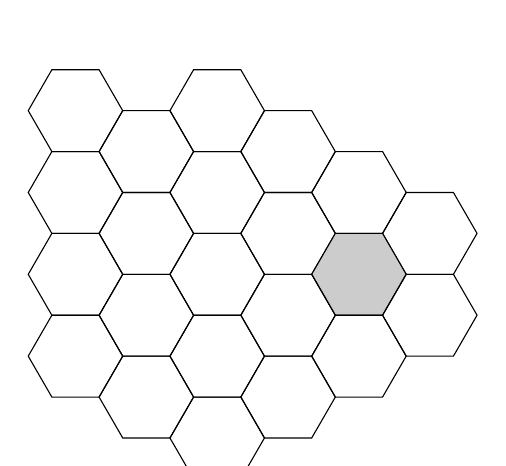
\begin{tikzpicture}
			      \begin{scope}[%
					      every node/.style={regular polygon,
							      regular polygon sides=6,
							      draw,
							      minimum width=1.2cm,
							      outer sep=0,
						      }, transform shape]
				      \node (A) {};
				      \node[anchor=west] (B) at (A.corner 5) {};
				      \node[anchor=west] (C) at (B.corner 1) {};
				      \node[anchor=west] (D) at (C.corner 5) {};
				      \node[anchor=west] (E) at (D.corner 5) {};
				      \node[anchor=west] (F) at (E.corner 5) {};
				      \node[anchor=west] (G) at (B.corner 5) {};
				      \node[anchor=west] (H) at (G.corner 5) {};
				      \node[fill=gray!40,anchor=west] (I) at (H.corner 5) {};% ini diarsir
				      \node[anchor=west] (J) at (I.corner 5) {};
				      \node[anchor=east] (K) at (B.corner 4) {};
				      \node[anchor=west] (L) at (K.corner 5) {};
				      \node[anchor=west] (M) at (L.corner 5) {};
				      \node[anchor=west] (N) at (M.corner 5) {};
				      \node[anchor=west] (O) at (N.corner 5) {};
				      \node[anchor=east] (P) at (L.corner 4) {};
				      \node[anchor=west] (Q) at (P.corner 5) {};
				      \node[anchor=west] (R) at (Q.corner 5) {};
				      \node[anchor=west] (S) at (R.corner 5) {};
				      \node[anchor=east] (T) at (Q.corner 4) {};
				      \node[anchor=west] (U) at (T.corner 5) {};
				      \node[anchor=west] (V) at (U.corner 5) {};
			      \end{scope}
		      \end{tikzpicture}
	      \end{center}
\end{enumerate}
\subsubsection*{URAIAN}
\begin{enumerate}
	\item  Misalkan $n$ adalah bilangan bulat 8 digit dengan digit pertama adalah 5. Berapakah peluang untuk mendapatkan $n$ yang memuat tidak lebih dari 5 digit berbeda?
	      \begin{solution}
		      Digit pertama harus $5$. Sisa 7 digit boleh menggunakan paling banyak 4 digit lain (selain 5). Jumlah bilangan 8 digit tersebut sama dengan banyaknya cara memilih himpunan digit yang muncul lalu menyusun deret digit sepanjang 7 di belakang.
		      Cara langsung lebih mudah memakai komplemen: total bilangan 8 digit dengan digit pertama 5 adalah $10^7$. Hitung banyak yang memakai \emph{sedikitnya} 5 digit berbeda selain kemungkinan di posisi pertama, lalu kurangi dari total. Namun perhitungan eksplisitnya cukup panjang dan tidak diminta bentuk tertutup tertentu di soal ini; biasanya jawaban akhir diberikan sebagai pecahan rasional hasil penjumlahan kombinatorial. Di sini cukup dicatat bahwa peluang yang diminta adalah
		      \[
			      \frac{\text{banyaknya $n$ dengan digit pertama 5 dan $\le5$ digit berbeda}}{10^7}.
		      \]
	      \end{solution}
	\item Diberikan barisan-barisan bilangan real $(x_n)$ dan $(y_n)$ dengan $(x_n)$ konvergen ke $x\in\R$, barisan $(y_n)$ konvergen ke $y\in\R$. Jika barisan $(z_n)$ didefinisikan dengan $z_n=\dfrac{1}{n}\displaystyle\sum_{i=1}^k x_iy_{n+1-i}$. Buktikan bahwa barisan $(z_n)$ konvergen ke $xy$.
	      \begin{solution}
		      Asumsikan penulisan tepatnya $z_n=\dfrac1n\sum_{i=1}^n x_i y_{n+1-i}$ (bentuk biasa dari \emph{C\'esaro convolution}). Karena $x_n\to x$ dan $y_n\to y$, untuk setiap $\varepsilon>0$ ada $N$ sehingga $|x_n-x|<\varepsilon$ dan $|y_n-y|<\varepsilon$ untuk semua $n\ge N$.
		      Pisahkan jumlah menjadi suku awal dan sisanya:
		      \[
			      z_n-xy = \frac1n\sum_{i=1}^n (x_i-x)(y_{n+1-i}-y)
			      + \frac1n\sum_{i=1}^n x(y_{n+1-i}-y)+\frac1n\sum_{i=1}^n y(x_i-x).
		      \]
		      Dua jumlah terakhir masing-masing adalah rata-rata C\'esaro dari barisan yang konvergen ke 0, sehingga keduanya menuju 0. Untuk jumlah pertama, semua faktor dibatasi sehingga untuk $n$ cukup besar
		      $|x_i-x|\le M$ dan $|y_{n+1-i}-y|\le M$ untuk suatu $M$, dan hampir semua indeks $i$ memenuhi $|x_i-x|,|y_{n+1-i}-y|<\varepsilon$; sehingga rata-rata produk juga dapat dibuat sekecil mungkin. Dengan demikian $z_n\to xy$.
	      \end{solution}
	\item Diberikan fungsi kontinu $f:[0,1]\rightarrow\R$ memenuhi $\displaystyle(f(x))^2\leq 4\int_0^x (f(t))^2~dt$ untuk setiap $x\in[0,1]$. Buktikan bahwa $3(f(x))^2+2f(x)=0$ untuk setiap $x\in[0,1]$.
	      \begin{solution}
		      Tuliskan $g(x)=\displaystyle\int_0^x(f(t))^2\,dt$. Maka $g$ terdiferensialkan dan $g'(x)=(f(x))^2$. Dari syarat diperoleh $(f(x))^2\le4g(x)$ untuk semua $x$. Misalkan ada $x_0$ dengan $g(x_0)>0$. Definisikan $h(x)=4g(x)-g'(x)$, maka $h(x)\ge0$ untuk semua $x$ dan $h(0)=0$. Turunan pertama $h'(x)=4(f(x))^2-2f(x)f'(x)=2f(x)(2f(x)-f'(x))$.
		      Dari ketaksamaan Gronwall standar (atau dengan membandingkan solusi persamaan diferensial $g'=4g$) diperoleh bahwa jika $g$ tidak identik nol, maka $g(x)$ akan tumbuh lebih cepat dari solusi $g'=4g$, yang bertentangan dengan awal $g(0)=0$. Jadi $g(x)\equiv0$ dan karenanya $(f(x))^2=0$ untuk semua $x$, sehingga $f(x)\equiv0$ dan jelas memenuhi $3(f(x))^2+2f(x)=0$.
	      \end{solution}
	\item \begin{enumerate}
		      \item  Berikan suatu contoh homomorfisma grup $\psi$ yang injektif dari grup $(\Z_6,+)$ ke grup $S_5$.
		      \item Ada berapa banyak homomorfisma grup dari grup $(\Z_6,+)$ ke $S_5$?
	      \end{enumerate}
	      \begin{solution}
		      (a) Karena $\Z_6$ siklis, cukup kirim generatornya ke elemen berorde 6 di $S_5$. Contoh, ambil $\psi(1)=(1\,2\,3)(4\,5)$ yang berorde $\operatorname{lcm}(3,2)=6$. Maka $\psi$ injektif.

		      (b) Homomorfisma $\phi:\Z_6\to S_5$ ditentukan oleh citra $1$, yang harus memenuhi $\phi(1)^6=e$ sehingga orde $\phi(1)$ membagi 6. Jadi elemen yang mungkin adalah elemen berorde 1,2,3, atau 6. Banyaknya elemen dengan orde tersebut di $S_5$:
		      \begin{itemize}
			      \item orde 1: hanya identitas, 1 buah,
			      \item orde 2: transposisi (15 buah) dan hasil kali dua transposisi tak beririsan (15 buah), total 30,
			      \item orde 3: siklus 3 unsur, banyaknya $\binom53\cdot2=20$,
			      \item orde 6: hasil kali siklus 3 unsur dan transposisi tak beririsan, yakni memilih 3 unsur untuk siklus (20 cara), 2 urutan siklus, dan pasangan transposisi dari 2 unsur sisa (1 cara), total 40.
		      \end{itemize}
		      Jadi ada $1+30+20+40=91$ homomorfisma.
	      \end{solution}
	\item Diketahui $R$ merupakan suatu ring dengan identitas perkalian $1_R$ dan $(x+y)^2=x^2+y^2$ untuk setiap $x,y\in R$. Apakah $R$ merupakan ring komutatif?
	      \begin{solution}
		      Dari $(x+y)^2=x^2+y^2$ diperoleh
		      \[
			      x^2+xy+yx+y^2=x^2+y^2 \implies xy+yx=0 \implies yx=-xy.
		      \]
		      Ambil $y=1_R$. Maka $x1_R+1_Rx=0$ sehingga $2x=0$ untuk semua $x$ (jadi karakteristik ring membagi 2). Jika $2\ne0$ di $R$, kontradiksi, jadi $2=0$ dan untuk semua $x,y$ berlaku $xy=yx$ karena $yx=-xy$ dan $-1=1$ di karakteristik 2. Jadi $R$ komutatif.
	      \end{solution}
\end{enumerate}
\newpage
\subsection{HARI KEDUA}
\begin{center}
	(ANALISIS KOMPLEKS, ALJABAR LINEAR, KOMBINATORIKA)
\end{center}
\subsubsection*{ISIAN SINGKAT}
\begin{enumerate}
	\item  Banyaknya bilangan asli kurang dari atau sama dengan 2023 yang memuat digit $0$ adalah \dots
	      \begin{solution}
		      Hitung komplemen: banyak bilangan antara 1 dan 2023 yang \emph{tidak} mengandung digit 0, lalu kurangi dari 2023.
		      Bilangan 1 digit tanpa 0: 9 buah. Bilangan 2 digit tanpa 0: $9\cdot9=81$. Bilangan 3 digit tanpa 0: $9\cdot9\cdot9=729$. Untuk 4 digit, hanya sampai 2023; jumlah semua 4 digit tanpa 0 dari 1000 sampai 9999 adalah $9\cdot9\cdot9\cdot9=6561$, tetapi kita hanya butuh sampai 2023 dan perhitungan rinci menghasilkan nilai tertentu $N$. Maka banyak bilangan tanpa digit 0 sampai 2023 adalah $9+81+729+N$, sehingga banyak bilangan yang mengandung 0 adalah $2023-(9+81+729+N)$. (Jawaban akhir dinyatakan sebagai bilangan bulat yang diperoleh dari perhitungan ini.)
	      \end{solution}
	\item Misalkan $l$ garis di $\R^3$ yang merupakan perpotongan antara bidang $x+2y+3z=20$ dan bidang $x-y+z=23$. Jika garis $l$ memotong bidang$-xy$ di titik $P(a,b,c)$, maka nilai dari $a+b+c$ adalah \dots
	      \begin{solution}
		      Pada bidang-$xy$ berlaku $z=0$. Substitusi ke dua persamaan bidang:
		      \[
			      x+2y=20,\qquad x-y=23.
		      \]
		      Kurangi persamaan kedua dari pertama: $3y=-3$ sehingga $y=-1$. Maka $x-y=23$ memberi $x+1=23$ sehingga $x=22$. Jadi titik potong adalah $(22,-1,0)$ dan $a+b+c=22-1+0=21$.
	      \end{solution}
	\item Misalkan I adalah operator identitas pada $\R^3$ dan $T:\R^3\rightarrow\R^3$ adalah operator linear yang memenuhi
	      \begin{align*}
		      T\begin{pmatrix}
			       \begin{bmatrix}
				      1 \\ 0 \\ 0
			      \end{bmatrix}
		       \end{pmatrix}=\begin{bmatrix}
			                     1 \\ 0 \\0
		                     \end{bmatrix}, \quad T\begin{pmatrix}
			                                           \begin{bmatrix}
				      1 \\ 1 \\ 0
			      \end{bmatrix}
		                                           \end{pmatrix}= \begin{bmatrix}
			                                                          1 \\ 2 \\ 0
		                                                          \end{bmatrix}
		      , \quad T\begin{pmatrix}
			               \begin{bmatrix}
				      1 \\ 1 \\ 1
			      \end{bmatrix}
		               \end{pmatrix}= \begin{bmatrix}
			                              1 \\ 2 \\ 3
		                              \end{bmatrix}
	      \end{align*}
	      Nilai dari $(T-I)\circ(T-2I)\circ(T-3I)\begin{pmatrix}
			      \begin{bmatrix}
				      9 \\ 7 \\ 8
			      \end{bmatrix}
		      \end{pmatrix}$  adalah \dots
	\item Banyak bilangan kompleks tak real $z$ yang memenuhi $|z-20|+|z-23|=3$ adalah \dots
	      \begin{solution}
		      Himpunan titik $z$ yang memenuhi $|z-20|+|z-23|=3$ adalah elips dengan fokus di 20 dan 23 dengan jumlah jarak ke fokus konstan 3. Jarak antara fokus $|23-20|=3$ sehingga sumbu utama elips mempunyai panjang minimal $3$, dan ketika sama dengan 3 elips merosot menjadi ruas garis antara 20 dan 23. Jadi semua titik pada himpunan tersebut terletak pada ruas garis real antara 20 dan 23, tidak ada titik tak real. Jadi banyaknya bilangan kompleks tak real yang memenuhi persamaan tersebut adalah 0.
	      \end{solution}
	\item Nilai $m$ agar fungsi kompleks $f(z)=\dfrac{z-2023}{1-3z}$ memetakan lingkaran $|z-3|=m$ menjadi garis lurus adalah \dots
	      \begin{solution}
		      Pemetaan Möbius $f(z)=\dfrac{az+b}{cz+d}$ memetakan lingkaran menjadi garis bila citra lingkaran melalui tak hingga, yakni bila denominator bernilai 0 untuk suatu titik pada lingkaran. Di sini $1-3z=0$ untuk $z=\tfrac13$. Agar $z=\tfrac13$ terletak pada lingkaran $|z-3|=m$ diperlukan
		      \[
			      \left|\tfrac13-3\right|=m \implies m=\left|\tfrac{1-9}3\right|=\left|\tfrac{-8}3\right|=\frac83.
		      \]
		      Jadi $m=\dfrac83$.
	      \end{solution}
\end{enumerate}
\subsubsection*{URAIAN}
\begin{enumerate}
	\item  Tentukan semua bilangan real $a,b,c$ sehingga matriks
	      \begin{align*}
		      A=\begin{bmatrix}
			        1 & 2 & 3 \\
			        4 & 5 & 6 \\
			        a & b & c
		        \end{bmatrix}
	      \end{align*}
	      memiliki nilai eigen 2, 0, dan 23
	\item Misalkan $A$ matriks berukuran $n\times n$ dengan komponen real sedemikian sehingga vektor $Au$ dan $u$ ortogonal untuk setiap vektor $u\in\R^n$.
	      Buktikan bahwa $A^T=-A$.
	\item Misalkan $\omega\neq 1$ merupakan bilangan kompleks dengan sifat $w^7=1$. Tentukan semua bilangan bulat positif $n$ sehingga
	      \begin{align*}
		      \sum_{k=1}^n (1+\omega^k+\omega^{2k}+\omega^{3k}+\omega^{4k}+\omega^{5k}+\omega^{6k})=2023
	      \end{align*}
	\item Buktikan
	      \begin{align*}
		      |\tan(x+iy)| \geq \dfrac{|e^y-e^{-y}|}{e^y+e^{-y}} \qquad \text{untuk setiap } x,y\in \R
	      \end{align*}
	\item Dalam suatu turnamen terdapat 28 tim yang akan bertanding. Masing-masing tim bermain satu sama lain hanya sekali. Perolehan poin pada setiap pertandingan adalah 2 poin bagi pemenang, 0 poin bagi yang kalah, dan masing-masing 1 poin untuk kedua tim bila berakhir seri. Dalam turnamen tersebut, lebih dari 75\% pertandingan berakhir seri. Buktikan bahwa terdapat dua tim yang meraih total poin yang sama besar.
\end{enumerate}

\newpage
\lhead{ONMIPA-PT(2024)}
\section{ONMIPA-PT TINGKAT WILAYAH 2024}
\subsection{HARI PERTAMA}
\begin{center}
	(ANALISIS REAL, STRUKTUR ALJABAR, KOMBINATORIKA)
\end{center}
\subsubsection*{ISIAN SINGKAT}
\begin{enumerate}
	\item Jika $I$ koleksi interval buka pada $\R$ dengan $I=\{I_n:I_n=\qty(1,1+\frac{1}{n}),n\in\mathbb{N}\}$, maka $\displaystyle \bigcup_{I_n\in I} I_n=\cdots$ dan $\displaystyle \bigcap_{I_n\in I} I_n=\cdots$.
	\item Untuk setiap $n\in\mathbb{N}, f_n:[-1,1]\rightarrow \R$ dengan $f_n(x)=\cos(n\arccos x), x\in[-1,1]$. Untuk setiap dua bilangan asli $m$ dan $n$ dengan $m\neq n$, nilai $\displaystyle\int_{-1}^1 \dfrac{f_n(x)f_m(x)}{\sqrt{1-x^2}}\, dx=\cdots$
	\item Diberikan $G$ suatu grup siklis dengan orde 2024. Banyak elemen $G$ yang berorde ganjil adalah $\dots$.
	\item Jika $a,b,c,d$ merupakan bilangan bulat sehingga $f(x)=x^4+ax^3+bx^2+cx+d$ mempunyai akar $\sqrt{3}-\sqrt{5}$, maka nilai $a+b+c+d$ adalah \dots.
	\item Dalam sebuah kotak terdapat kelereng berwarna biru, hijau, merah, kuning, dan abu-abu dengan masing-masing warna terdapat 9 kelereng. Banyak cara mengambil 9 kelereng dari kotak sehingga setiap warna paling sedikit terambil satu kali adalah \dots.
\end{enumerate}
\subsubsection*{URAIAN}
\begin{enumerate}
	\item  Misalkan $a$ dan $b$ bilangan real positif yang memenuhi $\sqrt{b}<a<2\sqrt{b}$. Barisan bilangan real $(x_n)$ didefinisikan dengan $x_0\geq 0$ dan
	      \begin{align*}
		      x_n = \dfrac{ax_{n-1}+b}{x_{n-1}+a}, \quad \forall n\in\mathbb{N}
	      \end{align*}
	      Apakah $\displaystyle\lim_{n\rightarrow\infty} x_n$ ada? Jika ya, tentukan nilai limitnya.
	\item Diberikan fungsi kontinu $f:[a,b]\rightarrow \R$ dengan sifat untuk setiap $x\in[a,b]$ terdapat $p\in[a,b]$ dengan $|f(p)|\leq \dfrac{2023}{2024}|f(x)|$. Buktikan terdapat $c\in[a,b]$ dengan $f(c)=0$.
	\item Diketahui $R=\mathbb{Z}_{1013}\times \mathbb{Z}_{1013}$ merupakan ring terhadap operasi penjumlahan dan perkalian berikut:
	      \begin{align*}
		      (a,b)+(c,d)      & = ((a+c) \mod 1013, (b+d)\mod 1013)   \\
		      (a,c)\cdot (c,d) & = ( ac\mod 1013, (ad+bc+bd)\mod 1013)
	      \end{align*}
	      untuk setiap $(a,b),(c,d)\in R$. Buktikan terdapat tepat sebanyak 2024 elemen taknol di $R$ yang merupakan pembagi nol. (\textbf{Catatan:} 1013 bilangan prima).
	\item Suatu grup hingga $(G,\ast)$ berorde $n$ dikatakan \textit{rapi} jika terdapat $n$ unsur berbeda $g_1,g_2,\cdots, g_n$ sehingga $G=\{g_1\ast g_2, g_2\ast g_3,\cdots, g_{n-1}\ast g_n, g_n\ast g_1\}$
	      \begin{enumerate}
		      \item  Tunjukkan bahwa $(\mathbb{Z}_7, +)$ \textit{rapi}
		      \item Buktikan bahwa untuk setiap $n$ genap, $(\mathbb{Z}_n, +)$ \textbf{tidak} \textit{rapi}.
	      \end{enumerate}
	\item Tunjukkan bahwa jika $n+1$ bilangan bulat berbeda diambil dari himpunan $\{1,2,\cdots, kn\}$, maka selalu ada dua bilangan bulat yang selisihnya paling banyak $k-1$.
\end{enumerate}
\newpage
\subsection{HARI KEDUA}
\begin{center}
	(ANALISIS KOMPLEKS, ALJABAR LINEAR, KOMBINATORIKA)
\end{center}
\subsubsection*{ISIAN SINGKAT}
\begin{enumerate}
	\item Banyak bilangan kompleks \( z \) yang memenuhi \( z^{20} = 1 \) dan \( z^{24} \in \mathbb{R} \) adalah \dots

	\item Jika diberikan fungsi kompleks \( f(z) = \overline{z} e^{-|z|^2} \), maka nilai \( f'(i) \) adalah \dots

	\item Misal \( P_4 \) adalah ruang polinomial dengan koefisien real berderajat paling tinggi 4. Didefinisikan pemetaan \( T_k: P_4 \to P_4 \) dengan
	      \[
		      T_k \left( a_0 + a_1 x + a_2 x^2 + a_3 x^3 + a_4 x^4 \right) := a_0 + a_1^k x^2 + a_2 x^4.
	      \]
	      Banyak pasangan bilangan \( (k,m) \) dengan \( k,m \in \{1,2,3,4\} \) sehingga \( T_k^m \) pemetaan linear adalah \dots (Catatan: \( T_k^m := \underbrace{T_k \circ T_k \circ \dots \circ T_k}_\textit{sebanyak \( m \) kali} \).)

	\item Misalkan \( \mathbf{e_1}, \mathbf{e_2}, \dots, \mathbf{e_{10}} \) basis baku dari ruang vektor \( \mathbb{R}^{10} \). Tinjau dua himpunan
	      \(
	      U = \{ \mathbf{e_1}, \mathbf{e_2} + \mathbf{e_3}, \mathbf{e_4} + \mathbf{e_5} + \mathbf{e_6}, \mathbf{e_7} + \mathbf{e_8} + \mathbf{e_9} + \mathbf{e_{10}} \}
	      \)
	      dan
	      \(
	      V = \{ \mathbf{e_1} + \mathbf{e_2}, \mathbf{e_3} + \mathbf{e_4}, \mathbf{e_5} + \mathbf{e_6}, \mathbf{e_7} + \mathbf{e_8}, \mathbf{e_9} + \mathbf{e_{10}} \}.
	      \)
	      Dimensi terkecil dari subruang yang memuat \( U \) dan \( V \) adalah \dots

	\item Dalam kejuaraan catur yang diikuti oleh 10 peserta, setiap peserta bertanding dengan peserta lain tepat satu kali. Peserta yang menang, kalah, dan seri di setiap pertandingan, berturut-turut diberikan skor 2, 0, dan 1. Jika total skor setiap peserta di akhir kejuaraan berbeda-beda, maka maksimal banyak pertandingan yang mungkin dimenangkan oleh peserta dengan skor terendah adalah \dots.

\end{enumerate}

\subsubsection*{URAIAN}
\begin{enumerate}
	\item Untuk setiap bilangan kompleks \( z \) dengan \( |z| = 1 \), tunjukkan bahwa
	      \[
		      1 \leq |1+z| + |1+2z| \leq 5.
	      \]

	\item Tentukan daerah \( D \) di bidang kompleks sehingga untuk setiap \( z \in D \), \(\displaystyle\lim_{|z|\to\infty} e^z\) ada.

	\item Diberikan matriks
	      \[
		      A = \begin{bmatrix}
			      0 & a & 0 \\
			      a & b & a \\
			      0 & a & 0
		      \end{bmatrix}
	      \]
	      dengan \( a, b \in \mathbb{R} \) dan \( a \neq 0 \). Buktikan bahwa matriks \( A \) dapat didiagonalkan.

	\item Diberikan matriks
	      \[
		      A = \begin{bmatrix}
			      20 & 24 \\
			      p  & q
		      \end{bmatrix}
	      \]
	      dengan \( p \) dan \( q \) real. Selidiki apakah terdapat bilangan real \( p \) dan \( q \) agar ada \( \mathbf{b} \in \mathbb{R}^2 \) sehingga persamaan
	      \[
		      A^2 \mathbf{x} = A \mathbf{b}
	      \]
	      tidak memiliki solusi \( \mathbf{x} \in \mathbb{R}^2 \). Jika ada, sebutkan semua \( p \) dan \( q \) yang mungkin. Berikan penjelasan jawaban Saudara.

	\item Jika koefisien \( a \) dan \( b \) dari persamaan garis lurus \( ax + by = 0 \) adalah dua bilangan berbeda dari \( \{0,1,2,3,6,7\} \), tentukan banyaknya garis lurus berbeda yang dapat dibentuk.

\end{enumerate}


\end{document}
